\chapter{Analysis of selected models}
\label{cha:analysis_of_selected_models}
\newpage
\begin{tcolorbox}[title={Contributions of this chapter}]
    The main contribution of this chapter is to apply the methods derived in \Cref{cha:state_space_models} to selected inference and prediction problems in the context of \acrshort{c19} in Germany.
    \paragraph{\nameref{sec:model_reporting_delay}}
    \phantom{stuff}
    \paragraph{\nameref{sec:regional_growth_factor_model}}
    \phantom{stuff}
    \paragraph{\nameref{sec:nowcasting_hospitalizations}}
    \phantom{stuff}
\end{tcolorbox}
\newpage
Equipped with the theoretical insight into the practical advantages that \acrshort{eis} has over the \acrshort{cem}, we are prepared to demonstrate the usefulness of \acrshortpl{ssm} for epidemiological modeling. To this end, we will present three applications where modeling with \acrshortpl{ssm} is useful: accounting for reporting artifacts (\Cref{sec:model_reporting_delay}) and regional effects (\Cref{sec:regional_growth_factor_model}), as well as fore- and nowcasting (\Cref{sec:nowcasting_hospitalizations}). In laying out the rationales for each of the models it will become clear that \acrshortpl{ssm} provide a flexible modeling framework that allows practitioners to tailor interpretable models to the question at hand. 

The models we present in this chapter are not based on compartmental models, but rather on the epidemiological indicators presented in \Cref{sec:measures_of_epidemic_spread}. We prefer these methods, as the compartmental models require their users to make a lot of assumptions regarding the dynamics of the epidemics, e.g. whether reinfections can or cannot occur, whether population size is fixed or not and also distributional assumptions for the rate of transitions between compartments. 
Such assumptions are hard to verify in practice and the influence of deviation from them is hard to quantify. Basing, the infection dynamics solely on the exponential growth factor only assumes that cases grow exponentially, which is theoretically and empirically straightforward to justify. 
Additionally, the parameters in compartmental models may be harder to interpret, compared to, e.g., the exponential growth factor, see \Cref{subsec:usefulness_of_indicators}.

Before we present our results, we give a short overview over similar work, in particular those that leverage \acrshortpl{ssm} to perform inference or short-term predictions for \acrshort{c19}. 

One prominent approach involves modeling disease dynamics through growth factors. \citep{Arroyo-Marioli2021Tracking} develop a local level model for the log-growth factor based on a classical SIR-model, which allows them to derive reproduction numbers. Their model is fully Gaussian and can be fit using the Kalman smoother. Similarly, \citep{Ives2021Estimating} present a similar local level model for the log-growth factor, but assume observations to follow a quasi-Poisson distribution, modeling the growth of deaths instead of reported cases. Their model is fit using the extended Kalman filter for the counties in the US.

An alternative strategy derives state space models directly from epidemiological theory. \citep{Lal2021Application} and \citep{Keller2022Tracking} derive \acrshortpl{ssm} from a time-discretized version of ODE-based compartmental models. In this framework, \citep{Lal2021Application} assume conditionally Gaussian observations, but the dependence between states and observations is non-linear, so they use the \acrshort{enkf} to fit the model. Taking a fully Bayesian perspective, \citep{Keller2022Tracking} use a negative binomial distribution for cases, hospitalizations and deaths. They adopt a fully Bayesian view putting priors on hyperparameters and derive posterior distributions of interest by Hamiltonian Monte-Carlo.

A third approach leverages asymptotic theory for computational efficiency. \citep{ODea2022Semiparametric} for example implement this approach, exploiting a \acrshort{clt} for compartmental models, to obtain a Gaussian approximation to the states' dynamics. The model can then be fit using the \acrshort{ekf}.

From this overview we see that many of the \acrshortpl{ssm} use compartmental models to model the epidemics' dynamics --- thus the models we present in this section provide an alternative way of modeling infectious disease data with simpler, interpretable models, giving practitioners more flexibility when choosing models to address their research questions.

\todo{all analyses on Macbook Air M3, if not noted otherwise, include computaiton time}
\section{Removing reporting delays and weekday effects}%
\label{sec:model_reporting_delay}
\subsection{Context}
\todo{rewrite: don't forecast, but use daily modeling as motivator}
Forecasting the number of new infections that will be reported in the coming days, weeks or months is one of the main tasks of epidemiological monitoring, see \Cref{sec:objectives}. However, as we have observed in \Cref{sec:data}, the data at our hand are contaminated by the reporting process, most notably the week-day effects, reporting delays, and artifacts due to public holidays.
While we can make the influence of these effects small by aggregating data to the weekly level, see \Cref{sec:regional_growth_factor_model}, modeling on the daily level has its merits: this is the smallest timescale data are available at, and so it should provide better predictions if we leverage the full information available. Additionally, going to the finest timescale possible is crucial if we are interested in quantifying the effects of \acrshortpl{npi}.
% ForecastHubs do weekly forecasting

% use RKI case data for whole country, split by reporting delay
In this section we use the \acrshort{rki} case incidence data discussed in \Cref{sec:data}. As we have seen in \Cref{fig:reporting_delays_cases} \textbf{A} and \Cref{fig:survival_function_rep_tri_incidences}, most delays are less than $4$ days. Thus, ignoring any cases reported with longer delays, we get for any reporting date $t$ four observations, say 
$$
    Y_{t} = \left( Y_{t, 1}, \dots, Y_{t, 4} \right) \in \N^{4}_{0}.
$$
Here $Y_{t,\tau}$, $\tau = 1, \dots, 4$, is the number of newly reported cases for reporting date $t$ with delay $\tau$, such that $Y_{t,\cdot} = \sum_{\tau = 1}^4 Y_{t, \tau}$ is the total number of cases reported for reporting date $t$ with delay $\leq 4$. 
Let $\hat p_{t, \tau} = \frac{Y_{t,\tau}}{Y_{t,\cdot}}$ be the empirical delay probability for day $t$ with delay $\tau$. We have already observed in \Cref{fig:reporting_delays_cases}, that $Y_{t, \cdot}$ is subject to weekday effects, and similar to hospitalizations (\Cref{fig:double_weekday_effect_hosp}), there is a small weekday effect for the delay of cases, i.e. $\hat p_{t,\tau}$, see \Cref{fig:weekday_effect_delays}. 

\begin{figure}
    \resizebox{\textwidth}{!}{%
        % Created by tikzDevice version 0.12.6 on 2024-08-27 13:02:34
% !TEX encoding = UTF-8 Unicode
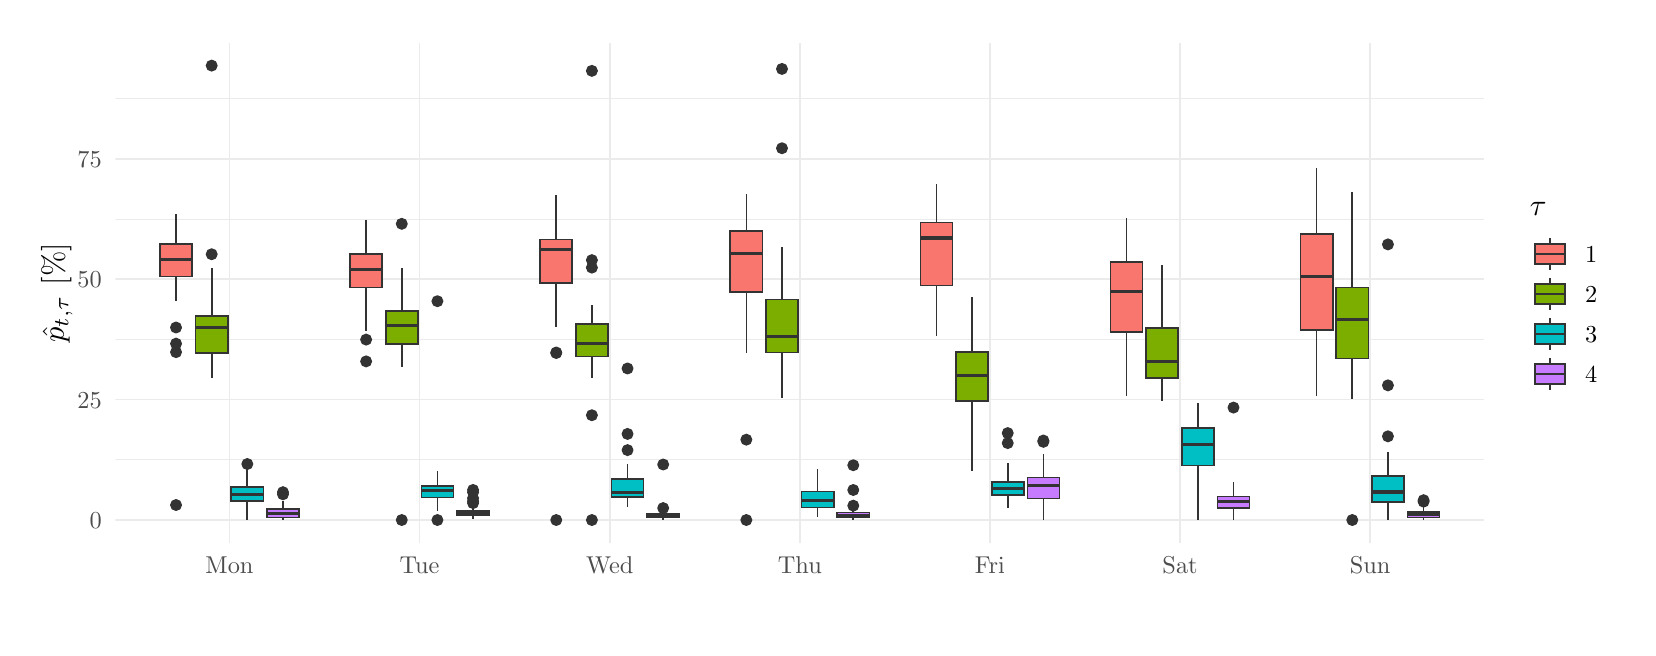
\begin{tikzpicture}[x=1pt,y=1pt]
\definecolor{fillColor}{RGB}{255,255,255}
\path[use as bounding box,fill=fillColor,fill opacity=0.00] (0,0) rectangle (578.16,216.81);
\begin{scope}
\path[clip] ( 31.71, 30.69) rectangle (526.31,211.31);
\definecolor{drawColor}{gray}{0.92}

\path[draw=drawColor,line width= 0.3pt,line join=round] ( 31.71, 60.64) --
	(526.31, 60.64);

\path[draw=drawColor,line width= 0.3pt,line join=round] ( 31.71,104.13) --
	(526.31,104.13);

\path[draw=drawColor,line width= 0.3pt,line join=round] ( 31.71,147.62) --
	(526.31,147.62);

\path[draw=drawColor,line width= 0.3pt,line join=round] ( 31.71,191.11) --
	(526.31,191.11);

\path[draw=drawColor,line width= 0.6pt,line join=round] ( 31.71, 38.90) --
	(526.31, 38.90);

\path[draw=drawColor,line width= 0.6pt,line join=round] ( 31.71, 82.39) --
	(526.31, 82.39);

\path[draw=drawColor,line width= 0.6pt,line join=round] ( 31.71,125.88) --
	(526.31,125.88);

\path[draw=drawColor,line width= 0.6pt,line join=round] ( 31.71,169.36) --
	(526.31,169.36);

\path[draw=drawColor,line width= 0.6pt,line join=round] ( 72.93, 30.69) --
	( 72.93,211.31);

\path[draw=drawColor,line width= 0.6pt,line join=round] (141.62, 30.69) --
	(141.62,211.31);

\path[draw=drawColor,line width= 0.6pt,line join=round] (210.32, 30.69) --
	(210.32,211.31);

\path[draw=drawColor,line width= 0.6pt,line join=round] (279.01, 30.69) --
	(279.01,211.31);

\path[draw=drawColor,line width= 0.6pt,line join=round] (347.70, 30.69) --
	(347.70,211.31);

\path[draw=drawColor,line width= 0.6pt,line join=round] (416.40, 30.69) --
	(416.40,211.31);

\path[draw=drawColor,line width= 0.6pt,line join=round] (485.09, 30.69) --
	(485.09,211.31);
\definecolor{drawColor}{gray}{0.20}
\definecolor{fillColor}{gray}{0.20}

\path[draw=drawColor,line width= 0.4pt,line join=round,line cap=round,fill=fillColor] ( 53.61,108.46) circle (  1.96);

\path[draw=drawColor,line width= 0.4pt,line join=round,line cap=round,fill=fillColor] ( 53.61,102.63) circle (  1.96);

\path[draw=drawColor,line width= 0.4pt,line join=round,line cap=round,fill=fillColor] ( 53.61, 99.56) circle (  1.96);

\path[draw=drawColor,line width= 0.4pt,line join=round,line cap=round,fill=fillColor] ( 53.61, 44.32) circle (  1.96);

\path[draw=drawColor,line width= 0.6pt,line join=round] ( 53.61,138.67) -- ( 53.61,149.60);

\path[draw=drawColor,line width= 0.6pt,line join=round] ( 53.61,126.86) -- ( 53.61,118.04);
\definecolor{fillColor}{RGB}{248,118,109}

\path[draw=drawColor,line width= 0.6pt,fill=fillColor] ( 47.81,138.67) --
	( 47.81,126.86) --
	( 59.40,126.86) --
	( 59.40,138.67) --
	( 47.81,138.67) --
	cycle;

\path[draw=drawColor,line width= 1.1pt] ( 47.81,133.04) -- ( 59.40,133.04);
\definecolor{fillColor}{gray}{0.20}

\path[draw=drawColor,line width= 0.4pt,line join=round,line cap=round,fill=fillColor] ( 66.49,134.94) circle (  1.96);

\path[draw=drawColor,line width= 0.4pt,line join=round,line cap=round,fill=fillColor] ( 66.49,203.10) circle (  1.96);

\path[draw=drawColor,line width= 0.6pt,line join=round] ( 66.49,112.55) -- ( 66.49,129.94);

\path[draw=drawColor,line width= 0.6pt,line join=round] ( 66.49, 99.20) -- ( 66.49, 90.37);
\definecolor{fillColor}{RGB}{124,174,0}

\path[draw=drawColor,line width= 0.6pt,fill=fillColor] ( 60.69,112.55) --
	( 60.69, 99.20) --
	( 72.28, 99.20) --
	( 72.28,112.55) --
	( 60.69,112.55) --
	cycle;

\path[draw=drawColor,line width= 1.1pt] ( 60.69,108.36) -- ( 72.28,108.36);
\definecolor{fillColor}{gray}{0.20}

\path[draw=drawColor,line width= 0.4pt,line join=round,line cap=round,fill=fillColor] ( 79.37, 59.14) circle (  1.96);

\path[draw=drawColor,line width= 0.6pt,line join=round] ( 79.37, 50.73) -- ( 79.37, 58.08);

\path[draw=drawColor,line width= 0.6pt,line join=round] ( 79.37, 45.68) -- ( 79.37, 38.90);
\definecolor{fillColor}{RGB}{0,191,196}

\path[draw=drawColor,line width= 0.6pt,fill=fillColor] ( 73.57, 50.73) --
	( 73.57, 45.68) --
	( 85.16, 45.68) --
	( 85.16, 50.73) --
	( 73.57, 50.73) --
	cycle;

\path[draw=drawColor,line width= 1.1pt] ( 73.57, 48.05) -- ( 85.16, 48.05);
\definecolor{fillColor}{gray}{0.20}

\path[draw=drawColor,line width= 0.4pt,line join=round,line cap=round,fill=fillColor] ( 92.25, 48.96) circle (  1.96);

\path[draw=drawColor,line width= 0.4pt,line join=round,line cap=round,fill=fillColor] ( 92.25, 48.19) circle (  1.96);

\path[draw=drawColor,line width= 0.6pt,line join=round] ( 92.25, 42.79) -- ( 92.25, 45.95);

\path[draw=drawColor,line width= 0.6pt,line join=round] ( 92.25, 39.80) -- ( 92.25, 38.90);
\definecolor{fillColor}{RGB}{199,124,255}

\path[draw=drawColor,line width= 0.6pt,fill=fillColor] ( 86.45, 42.79) --
	( 86.45, 39.80) --
	( 98.04, 39.80) --
	( 98.04, 42.79) --
	( 86.45, 42.79) --
	cycle;

\path[draw=drawColor,line width= 1.1pt] ( 86.45, 41.36) -- ( 98.04, 41.36);
\definecolor{fillColor}{gray}{0.20}

\path[draw=drawColor,line width= 0.4pt,line join=round,line cap=round,fill=fillColor] (122.30,104.09) circle (  1.96);

\path[draw=drawColor,line width= 0.4pt,line join=round,line cap=round,fill=fillColor] (122.30, 96.22) circle (  1.96);

\path[draw=drawColor,line width= 0.6pt,line join=round] (122.30,135.14) -- (122.30,147.36);

\path[draw=drawColor,line width= 0.6pt,line join=round] (122.30,122.87) -- (122.30,107.08);
\definecolor{fillColor}{RGB}{248,118,109}

\path[draw=drawColor,line width= 0.6pt,fill=fillColor] (116.51,135.14) --
	(116.51,122.87) --
	(128.10,122.87) --
	(128.10,135.14) --
	(116.51,135.14) --
	cycle;

\path[draw=drawColor,line width= 1.1pt] (116.51,129.28) -- (128.10,129.28);
\definecolor{fillColor}{gray}{0.20}

\path[draw=drawColor,line width= 0.4pt,line join=round,line cap=round,fill=fillColor] (135.18,145.93) circle (  1.96);

\path[draw=drawColor,line width= 0.4pt,line join=round,line cap=round,fill=fillColor] (135.18, 38.90) circle (  1.96);

\path[draw=drawColor,line width= 0.6pt,line join=round] (135.18,114.54) -- (135.18,130.07);

\path[draw=drawColor,line width= 0.6pt,line join=round] (135.18,102.42) -- (135.18, 94.15);
\definecolor{fillColor}{RGB}{124,174,0}

\path[draw=drawColor,line width= 0.6pt,fill=fillColor] (129.39,114.54) --
	(129.39,102.42) --
	(140.98,102.42) --
	(140.98,114.54) --
	(129.39,114.54) --
	cycle;

\path[draw=drawColor,line width= 1.1pt] (129.39,109.02) -- (140.98,109.02);
\definecolor{fillColor}{gray}{0.20}

\path[draw=drawColor,line width= 0.4pt,line join=round,line cap=round,fill=fillColor] (148.06,117.97) circle (  1.96);

\path[draw=drawColor,line width= 0.4pt,line join=round,line cap=round,fill=fillColor] (148.06, 38.90) circle (  1.96);

\path[draw=drawColor,line width= 0.6pt,line join=round] (148.06, 51.13) -- (148.06, 56.72);

\path[draw=drawColor,line width= 0.6pt,line join=round] (148.06, 47.00) -- (148.06, 42.04);
\definecolor{fillColor}{RGB}{0,191,196}

\path[draw=drawColor,line width= 0.6pt,fill=fillColor] (142.27, 51.13) --
	(142.27, 47.00) --
	(153.86, 47.00) --
	(153.86, 51.13) --
	(142.27, 51.13) --
	cycle;

\path[draw=drawColor,line width= 1.1pt] (142.27, 49.43) -- (153.86, 49.43);
\definecolor{fillColor}{gray}{0.20}

\path[draw=drawColor,line width= 0.4pt,line join=round,line cap=round,fill=fillColor] (160.94, 48.93) circle (  1.96);

\path[draw=drawColor,line width= 0.4pt,line join=round,line cap=round,fill=fillColor] (160.94, 49.77) circle (  1.96);

\path[draw=drawColor,line width= 0.4pt,line join=round,line cap=round,fill=fillColor] (160.94, 46.79) circle (  1.96);

\path[draw=drawColor,line width= 0.4pt,line join=round,line cap=round,fill=fillColor] (160.94, 45.01) circle (  1.96);

\path[draw=drawColor,line width= 0.4pt,line join=round,line cap=round,fill=fillColor] (160.94, 45.72) circle (  1.96);

\path[draw=drawColor,line width= 0.6pt,line join=round] (160.94, 42.16) -- (160.94, 44.42);

\path[draw=drawColor,line width= 0.6pt,line join=round] (160.94, 40.56) -- (160.94, 39.10);
\definecolor{fillColor}{RGB}{199,124,255}

\path[draw=drawColor,line width= 0.6pt,fill=fillColor] (155.15, 42.16) --
	(155.15, 40.56) --
	(166.74, 40.56) --
	(166.74, 42.16) --
	(155.15, 42.16) --
	cycle;

\path[draw=drawColor,line width= 1.1pt] (155.15, 41.22) -- (166.74, 41.22);
\definecolor{fillColor}{gray}{0.20}

\path[draw=drawColor,line width= 0.4pt,line join=round,line cap=round,fill=fillColor] (191.00, 99.43) circle (  1.96);

\path[draw=drawColor,line width= 0.4pt,line join=round,line cap=round,fill=fillColor] (191.00, 99.25) circle (  1.96);

\path[draw=drawColor,line width= 0.4pt,line join=round,line cap=round,fill=fillColor] (191.00, 38.90) circle (  1.96);

\path[draw=drawColor,line width= 0.6pt,line join=round] (191.00,140.27) -- (191.00,156.21);

\path[draw=drawColor,line width= 0.6pt,line join=round] (191.00,124.46) -- (191.00,108.72);
\definecolor{fillColor}{RGB}{248,118,109}

\path[draw=drawColor,line width= 0.6pt,fill=fillColor] (185.20,140.27) --
	(185.20,124.46) --
	(196.79,124.46) --
	(196.79,140.27) --
	(185.20,140.27) --
	cycle;

\path[draw=drawColor,line width= 1.1pt] (185.20,136.51) -- (196.79,136.51);
\definecolor{fillColor}{gray}{0.20}

\path[draw=drawColor,line width= 0.4pt,line join=round,line cap=round,fill=fillColor] (203.88,130.11) circle (  1.96);

\path[draw=drawColor,line width= 0.4pt,line join=round,line cap=round,fill=fillColor] (203.88,132.81) circle (  1.96);

\path[draw=drawColor,line width= 0.4pt,line join=round,line cap=round,fill=fillColor] (203.88, 76.77) circle (  1.96);

\path[draw=drawColor,line width= 0.4pt,line join=round,line cap=round,fill=fillColor] (203.88,201.20) circle (  1.96);

\path[draw=drawColor,line width= 0.4pt,line join=round,line cap=round,fill=fillColor] (203.88, 38.90) circle (  1.96);

\path[draw=drawColor,line width= 0.6pt,line join=round] (203.88,109.68) -- (203.88,116.57);

\path[draw=drawColor,line width= 0.6pt,line join=round] (203.88, 98.01) -- (203.88, 90.22);
\definecolor{fillColor}{RGB}{124,174,0}

\path[draw=drawColor,line width= 0.6pt,fill=fillColor] (198.08,109.68) --
	(198.08, 98.01) --
	(209.67, 98.01) --
	(209.67,109.68) --
	(198.08,109.68) --
	cycle;

\path[draw=drawColor,line width= 1.1pt] (198.08,102.76) -- (209.67,102.76);
\definecolor{fillColor}{gray}{0.20}

\path[draw=drawColor,line width= 0.4pt,line join=round,line cap=round,fill=fillColor] (216.76, 64.16) circle (  1.96);

\path[draw=drawColor,line width= 0.4pt,line join=round,line cap=round,fill=fillColor] (216.76, 70.01) circle (  1.96);

\path[draw=drawColor,line width= 0.4pt,line join=round,line cap=round,fill=fillColor] (216.76, 93.66) circle (  1.96);

\path[draw=drawColor,line width= 0.6pt,line join=round] (216.76, 53.72) -- (216.76, 59.24);

\path[draw=drawColor,line width= 0.6pt,line join=round] (216.76, 47.22) -- (216.76, 43.53);
\definecolor{fillColor}{RGB}{0,191,196}

\path[draw=drawColor,line width= 0.6pt,fill=fillColor] (210.96, 53.72) --
	(210.96, 47.22) --
	(222.55, 47.22) --
	(222.55, 53.72) --
	(210.96, 53.72) --
	cycle;

\path[draw=drawColor,line width= 1.1pt] (210.96, 48.99) -- (222.55, 48.99);
\definecolor{fillColor}{gray}{0.20}

\path[draw=drawColor,line width= 0.4pt,line join=round,line cap=round,fill=fillColor] (229.64, 58.96) circle (  1.96);

\path[draw=drawColor,line width= 0.4pt,line join=round,line cap=round,fill=fillColor] (229.64, 43.21) circle (  1.96);

\path[draw=drawColor,line width= 0.6pt,line join=round] (229.64, 41.12) -- (229.64, 42.34);

\path[draw=drawColor,line width= 0.6pt,line join=round] (229.64, 39.90) -- (229.64, 38.90);
\definecolor{fillColor}{RGB}{199,124,255}

\path[draw=drawColor,line width= 0.6pt,fill=fillColor] (223.84, 41.12) --
	(223.84, 39.90) --
	(235.43, 39.90) --
	(235.43, 41.12) --
	(223.84, 41.12) --
	cycle;

\path[draw=drawColor,line width= 1.1pt] (223.84, 40.45) -- (235.43, 40.45);
\definecolor{fillColor}{gray}{0.20}

\path[draw=drawColor,line width= 0.4pt,line join=round,line cap=round,fill=fillColor] (259.69, 67.93) circle (  1.96);

\path[draw=drawColor,line width= 0.4pt,line join=round,line cap=round,fill=fillColor] (259.69, 38.90) circle (  1.96);

\path[draw=drawColor,line width= 0.6pt,line join=round] (259.69,143.45) -- (259.69,156.54);

\path[draw=drawColor,line width= 0.6pt,line join=round] (259.69,121.36) -- (259.69, 99.37);
\definecolor{fillColor}{RGB}{248,118,109}

\path[draw=drawColor,line width= 0.6pt,fill=fillColor] (253.89,143.45) --
	(253.89,121.36) --
	(265.49,121.36) --
	(265.49,143.45) --
	(253.89,143.45) --
	cycle;

\path[draw=drawColor,line width= 1.1pt] (253.89,135.11) -- (265.49,135.11);
\definecolor{fillColor}{gray}{0.20}

\path[draw=drawColor,line width= 0.4pt,line join=round,line cap=round,fill=fillColor] (272.57,173.24) circle (  1.96);

\path[draw=drawColor,line width= 0.4pt,line join=round,line cap=round,fill=fillColor] (272.57,201.90) circle (  1.96);

\path[draw=drawColor,line width= 0.6pt,line join=round] (272.57,118.55) -- (272.57,137.57);

\path[draw=drawColor,line width= 0.6pt,line join=round] (272.57, 99.49) -- (272.57, 82.99);
\definecolor{fillColor}{RGB}{124,174,0}

\path[draw=drawColor,line width= 0.6pt,fill=fillColor] (266.77,118.55) --
	(266.77, 99.49) --
	(278.37, 99.49) --
	(278.37,118.55) --
	(266.77,118.55) --
	cycle;

\path[draw=drawColor,line width= 1.1pt] (266.77,105.38) -- (278.37,105.38);

\path[draw=drawColor,line width= 0.6pt,line join=round] (285.45, 49.23) -- (285.45, 57.20);

\path[draw=drawColor,line width= 0.6pt,line join=round] (285.45, 43.42) -- (285.45, 39.88);
\definecolor{fillColor}{RGB}{0,191,196}

\path[draw=drawColor,line width= 0.6pt,fill=fillColor] (279.65, 49.23) --
	(279.65, 43.42) --
	(291.25, 43.42) --
	(291.25, 49.23) --
	(279.65, 49.23) --
	cycle;

\path[draw=drawColor,line width= 1.1pt] (279.65, 45.80) -- (291.25, 45.80);
\definecolor{fillColor}{gray}{0.20}

\path[draw=drawColor,line width= 0.4pt,line join=round,line cap=round,fill=fillColor] (298.33, 44.09) circle (  1.96);

\path[draw=drawColor,line width= 0.4pt,line join=round,line cap=round,fill=fillColor] (298.33, 49.75) circle (  1.96);

\path[draw=drawColor,line width= 0.4pt,line join=round,line cap=round,fill=fillColor] (298.33, 58.70) circle (  1.96);

\path[draw=drawColor,line width= 0.6pt,line join=round] (298.33, 41.66) -- (298.33, 43.75);

\path[draw=drawColor,line width= 0.6pt,line join=round] (298.33, 40.06) -- (298.33, 38.90);
\definecolor{fillColor}{RGB}{199,124,255}

\path[draw=drawColor,line width= 0.6pt,fill=fillColor] (292.53, 41.66) --
	(292.53, 40.06) --
	(304.13, 40.06) --
	(304.13, 41.66) --
	(292.53, 41.66) --
	cycle;

\path[draw=drawColor,line width= 1.1pt] (292.53, 40.70) -- (304.13, 40.70);

\path[draw=drawColor,line width= 0.6pt,line join=round] (328.38,146.40) -- (328.38,160.14);

\path[draw=drawColor,line width= 0.6pt,line join=round] (328.38,123.66) -- (328.38,105.35);
\definecolor{fillColor}{RGB}{248,118,109}

\path[draw=drawColor,line width= 0.6pt,fill=fillColor] (322.59,146.40) --
	(322.59,123.66) --
	(334.18,123.66) --
	(334.18,146.40) --
	(322.59,146.40) --
	cycle;

\path[draw=drawColor,line width= 1.1pt] (322.59,140.80) -- (334.18,140.80);

\path[draw=drawColor,line width= 0.6pt,line join=round] (341.26, 99.65) -- (341.26,119.60);

\path[draw=drawColor,line width= 0.6pt,line join=round] (341.26, 81.98) -- (341.26, 56.47);
\definecolor{fillColor}{RGB}{124,174,0}

\path[draw=drawColor,line width= 0.6pt,fill=fillColor] (335.47, 99.65) --
	(335.47, 81.98) --
	(347.06, 81.98) --
	(347.06, 99.65) --
	(335.47, 99.65) --
	cycle;

\path[draw=drawColor,line width= 1.1pt] (335.47, 91.20) -- (347.06, 91.20);
\definecolor{fillColor}{gray}{0.20}

\path[draw=drawColor,line width= 0.4pt,line join=round,line cap=round,fill=fillColor] (354.14, 66.70) circle (  1.96);

\path[draw=drawColor,line width= 0.4pt,line join=round,line cap=round,fill=fillColor] (354.14, 70.31) circle (  1.96);

\path[draw=drawColor,line width= 0.6pt,line join=round] (354.14, 52.68) -- (354.14, 59.36);

\path[draw=drawColor,line width= 0.6pt,line join=round] (354.14, 47.97) -- (354.14, 43.12);
\definecolor{fillColor}{RGB}{0,191,196}

\path[draw=drawColor,line width= 0.6pt,fill=fillColor] (348.35, 52.68) --
	(348.35, 47.97) --
	(359.94, 47.97) --
	(359.94, 52.68) --
	(348.35, 52.68) --
	cycle;

\path[draw=drawColor,line width= 1.1pt] (348.35, 50.20) -- (359.94, 50.20);
\definecolor{fillColor}{gray}{0.20}

\path[draw=drawColor,line width= 0.4pt,line join=round,line cap=round,fill=fillColor] (367.02, 67.15) circle (  1.96);

\path[draw=drawColor,line width= 0.4pt,line join=round,line cap=round,fill=fillColor] (367.02, 67.63) circle (  1.96);

\path[draw=drawColor,line width= 0.6pt,line join=round] (367.02, 54.31) -- (367.02, 62.79);

\path[draw=drawColor,line width= 0.6pt,line join=round] (367.02, 46.69) -- (367.02, 38.90);
\definecolor{fillColor}{RGB}{199,124,255}

\path[draw=drawColor,line width= 0.6pt,fill=fillColor] (361.23, 54.31) --
	(361.23, 46.69) --
	(372.82, 46.69) --
	(372.82, 54.31) --
	(361.23, 54.31) --
	cycle;

\path[draw=drawColor,line width= 1.1pt] (361.23, 51.51) -- (372.82, 51.51);

\path[draw=drawColor,line width= 0.6pt,line join=round] (397.08,132.11) -- (397.08,147.94);

\path[draw=drawColor,line width= 0.6pt,line join=round] (397.08,106.78) -- (397.08, 83.54);
\definecolor{fillColor}{RGB}{248,118,109}

\path[draw=drawColor,line width= 0.6pt,fill=fillColor] (391.28,132.11) --
	(391.28,106.78) --
	(402.87,106.78) --
	(402.87,132.11) --
	(391.28,132.11) --
	cycle;

\path[draw=drawColor,line width= 1.1pt] (391.28,121.56) -- (402.87,121.56);

\path[draw=drawColor,line width= 0.6pt,line join=round] (409.96,108.34) -- (409.96,131.15);

\path[draw=drawColor,line width= 0.6pt,line join=round] (409.96, 90.28) -- (409.96, 81.74);
\definecolor{fillColor}{RGB}{124,174,0}

\path[draw=drawColor,line width= 0.6pt,fill=fillColor] (404.16,108.34) --
	(404.16, 90.28) --
	(415.75, 90.28) --
	(415.75,108.34) --
	(404.16,108.34) --
	cycle;

\path[draw=drawColor,line width= 1.1pt] (404.16, 96.26) -- (415.75, 96.26);

\path[draw=drawColor,line width= 0.6pt,line join=round] (422.84, 72.12) -- (422.84, 81.35);

\path[draw=drawColor,line width= 0.6pt,line join=round] (422.84, 58.64) -- (422.84, 38.90);
\definecolor{fillColor}{RGB}{0,191,196}

\path[draw=drawColor,line width= 0.6pt,fill=fillColor] (417.04, 72.12) --
	(417.04, 58.64) --
	(428.63, 58.64) --
	(428.63, 72.12) --
	(417.04, 72.12) --
	cycle;

\path[draw=drawColor,line width= 1.1pt] (417.04, 66.08) -- (428.63, 66.08);
\definecolor{fillColor}{gray}{0.20}

\path[draw=drawColor,line width= 0.4pt,line join=round,line cap=round,fill=fillColor] (435.72, 79.53) circle (  1.96);

\path[draw=drawColor,line width= 0.6pt,line join=round] (435.72, 47.42) -- (435.72, 52.60);

\path[draw=drawColor,line width= 0.6pt,line join=round] (435.72, 43.26) -- (435.72, 38.90);
\definecolor{fillColor}{RGB}{199,124,255}

\path[draw=drawColor,line width= 0.6pt,fill=fillColor] (429.92, 47.42) --
	(429.92, 43.26) --
	(441.51, 43.26) --
	(441.51, 47.42) --
	(429.92, 47.42) --
	cycle;

\path[draw=drawColor,line width= 1.1pt] (429.92, 45.46) -- (441.51, 45.46);

\path[draw=drawColor,line width= 0.6pt,line join=round] (465.77,142.34) -- (465.77,165.99);

\path[draw=drawColor,line width= 0.6pt,line join=round] (465.77,107.53) -- (465.77, 83.76);
\definecolor{fillColor}{RGB}{248,118,109}

\path[draw=drawColor,line width= 0.6pt,fill=fillColor] (459.97,142.34) --
	(459.97,107.53) --
	(471.57,107.53) --
	(471.57,142.34) --
	(459.97,142.34) --
	cycle;

\path[draw=drawColor,line width= 1.1pt] (459.97,126.95) -- (471.57,126.95);
\definecolor{fillColor}{gray}{0.20}

\path[draw=drawColor,line width= 0.4pt,line join=round,line cap=round,fill=fillColor] (478.65, 38.90) circle (  1.96);

\path[draw=drawColor,line width= 0.6pt,line join=round] (478.65,122.90) -- (478.65,157.31);

\path[draw=drawColor,line width= 0.6pt,line join=round] (478.65, 97.22) -- (478.65, 82.58);
\definecolor{fillColor}{RGB}{124,174,0}

\path[draw=drawColor,line width= 0.6pt,fill=fillColor] (472.85,122.90) --
	(472.85, 97.22) --
	(484.45, 97.22) --
	(484.45,122.90) --
	(472.85,122.90) --
	cycle;

\path[draw=drawColor,line width= 1.1pt] (472.85,111.47) -- (484.45,111.47);
\definecolor{fillColor}{gray}{0.20}

\path[draw=drawColor,line width= 0.4pt,line join=round,line cap=round,fill=fillColor] (491.53, 87.56) circle (  1.96);

\path[draw=drawColor,line width= 0.4pt,line join=round,line cap=round,fill=fillColor] (491.53,138.49) circle (  1.96);

\path[draw=drawColor,line width= 0.4pt,line join=round,line cap=round,fill=fillColor] (491.53, 69.14) circle (  1.96);

\path[draw=drawColor,line width= 0.6pt,line join=round] (491.53, 54.70) -- (491.53, 63.51);

\path[draw=drawColor,line width= 0.6pt,line join=round] (491.53, 45.38) -- (491.53, 38.90);
\definecolor{fillColor}{RGB}{0,191,196}

\path[draw=drawColor,line width= 0.6pt,fill=fillColor] (485.73, 54.70) --
	(485.73, 45.38) --
	(497.33, 45.38) --
	(497.33, 54.70) --
	(485.73, 54.70) --
	cycle;

\path[draw=drawColor,line width= 1.1pt] (485.73, 49.03) -- (497.33, 49.03);
\definecolor{fillColor}{gray}{0.20}

\path[draw=drawColor,line width= 0.4pt,line join=round,line cap=round,fill=fillColor] (504.41, 46.07) circle (  1.96);

\path[draw=drawColor,line width= 0.4pt,line join=round,line cap=round,fill=fillColor] (504.41, 45.54) circle (  1.96);

\path[draw=drawColor,line width= 0.6pt,line join=round] (504.41, 41.73) -- (504.41, 43.83);

\path[draw=drawColor,line width= 0.6pt,line join=round] (504.41, 39.85) -- (504.41, 38.90);
\definecolor{fillColor}{RGB}{199,124,255}

\path[draw=drawColor,line width= 0.6pt,fill=fillColor] (498.61, 41.73) --
	(498.61, 39.85) --
	(510.21, 39.85) --
	(510.21, 41.73) --
	(498.61, 41.73) --
	cycle;

\path[draw=drawColor,line width= 1.1pt] (498.61, 40.90) -- (510.21, 40.90);
\end{scope}
\begin{scope}
\path[clip] (  0.00,  0.00) rectangle (578.16,216.81);
\definecolor{drawColor}{gray}{0.30}

\node[text=drawColor,anchor=base east,inner sep=0pt, outer sep=0pt, scale=  0.88] at ( 26.76, 35.87) {0};

\node[text=drawColor,anchor=base east,inner sep=0pt, outer sep=0pt, scale=  0.88] at ( 26.76, 79.36) {25};

\node[text=drawColor,anchor=base east,inner sep=0pt, outer sep=0pt, scale=  0.88] at ( 26.76,122.84) {50};

\node[text=drawColor,anchor=base east,inner sep=0pt, outer sep=0pt, scale=  0.88] at ( 26.76,166.33) {75};
\end{scope}
\begin{scope}
\path[clip] (  0.00,  0.00) rectangle (578.16,216.81);
\definecolor{drawColor}{gray}{0.30}

\node[text=drawColor,anchor=base,inner sep=0pt, outer sep=0pt, scale=  0.88] at ( 72.93, 19.68) {Mon};

\node[text=drawColor,anchor=base,inner sep=0pt, outer sep=0pt, scale=  0.88] at (141.62, 19.68) {Tue};

\node[text=drawColor,anchor=base,inner sep=0pt, outer sep=0pt, scale=  0.88] at (210.32, 19.68) {Wed};

\node[text=drawColor,anchor=base,inner sep=0pt, outer sep=0pt, scale=  0.88] at (279.01, 19.68) {Thu};

\node[text=drawColor,anchor=base,inner sep=0pt, outer sep=0pt, scale=  0.88] at (347.70, 19.68) {Fri};

\node[text=drawColor,anchor=base,inner sep=0pt, outer sep=0pt, scale=  0.88] at (416.40, 19.68) {Sat};

\node[text=drawColor,anchor=base,inner sep=0pt, outer sep=0pt, scale=  0.88] at (485.09, 19.68) {Sun};
\end{scope}
\begin{scope}
\path[clip] (  0.00,  0.00) rectangle (578.16,216.81);
\definecolor{drawColor}{RGB}{0,0,0}

\node[text=drawColor,rotate= 90.00,anchor=base,inner sep=0pt, outer sep=0pt, scale=  1.10] at ( 13.08,121.00) {$\hat p_{t, \tau}$ [\%]};
\end{scope}
\begin{scope}
\path[clip] (  0.00,  0.00) rectangle (578.16,216.81);
\definecolor{drawColor}{RGB}{0,0,0}

\node[text=drawColor,anchor=base west,inner sep=0pt, outer sep=0pt, scale=  1.10] at (542.81,148.87) {$\tau$};
\end{scope}
\begin{scope}
\path[clip] (  0.00,  0.00) rectangle (578.16,216.81);
\definecolor{drawColor}{gray}{0.20}

\path[draw=drawColor,line width= 0.6pt] (550.03,129.29) --
	(550.03,131.46);

\path[draw=drawColor,line width= 0.6pt] (550.03,138.69) --
	(550.03,140.85);
\definecolor{fillColor}{RGB}{248,118,109}

\path[draw=drawColor,line width= 0.6pt,fill=fillColor] (544.61,131.46) rectangle (555.45,138.69);

\path[draw=drawColor,line width= 0.6pt] (544.61,135.07) --
	(555.45,135.07);
\end{scope}
\begin{scope}
\path[clip] (  0.00,  0.00) rectangle (578.16,216.81);
\definecolor{drawColor}{gray}{0.20}

\path[draw=drawColor,line width= 0.6pt] (550.03,114.84) --
	(550.03,117.00);

\path[draw=drawColor,line width= 0.6pt] (550.03,124.23) --
	(550.03,126.40);
\definecolor{fillColor}{RGB}{124,174,0}

\path[draw=drawColor,line width= 0.6pt,fill=fillColor] (544.61,117.00) rectangle (555.45,124.23);

\path[draw=drawColor,line width= 0.6pt] (544.61,120.62) --
	(555.45,120.62);
\end{scope}
\begin{scope}
\path[clip] (  0.00,  0.00) rectangle (578.16,216.81);
\definecolor{drawColor}{gray}{0.20}

\path[draw=drawColor,line width= 0.6pt] (550.03,100.38) --
	(550.03,102.55);

\path[draw=drawColor,line width= 0.6pt] (550.03,109.78) --
	(550.03,111.95);
\definecolor{fillColor}{RGB}{0,191,196}

\path[draw=drawColor,line width= 0.6pt,fill=fillColor] (544.61,102.55) rectangle (555.45,109.78);

\path[draw=drawColor,line width= 0.6pt] (544.61,106.16) --
	(555.45,106.16);
\end{scope}
\begin{scope}
\path[clip] (  0.00,  0.00) rectangle (578.16,216.81);
\definecolor{drawColor}{gray}{0.20}

\path[draw=drawColor,line width= 0.6pt] (550.03, 85.93) --
	(550.03, 88.10);

\path[draw=drawColor,line width= 0.6pt] (550.03, 95.32) --
	(550.03, 97.49);
\definecolor{fillColor}{RGB}{199,124,255}

\path[draw=drawColor,line width= 0.6pt,fill=fillColor] (544.61, 88.10) rectangle (555.45, 95.32);

\path[draw=drawColor,line width= 0.6pt] (544.61, 91.71) --
	(555.45, 91.71);
\end{scope}
\begin{scope}
\path[clip] (  0.00,  0.00) rectangle (578.16,216.81);
\definecolor{drawColor}{RGB}{0,0,0}

\node[text=drawColor,anchor=base west,inner sep=0pt, outer sep=0pt, scale=  0.88] at (562.76,132.04) {1};
\end{scope}
\begin{scope}
\path[clip] (  0.00,  0.00) rectangle (578.16,216.81);
\definecolor{drawColor}{RGB}{0,0,0}

\node[text=drawColor,anchor=base west,inner sep=0pt, outer sep=0pt, scale=  0.88] at (562.76,117.59) {2};
\end{scope}
\begin{scope}
\path[clip] (  0.00,  0.00) rectangle (578.16,216.81);
\definecolor{drawColor}{RGB}{0,0,0}

\node[text=drawColor,anchor=base west,inner sep=0pt, outer sep=0pt, scale=  0.88] at (562.76,103.13) {3};
\end{scope}
\begin{scope}
\path[clip] (  0.00,  0.00) rectangle (578.16,216.81);
\definecolor{drawColor}{RGB}{0,0,0}

\node[text=drawColor,anchor=base west,inner sep=0pt, outer sep=0pt, scale=  0.88] at (562.76, 88.68) {4};
\end{scope}
\end{tikzpicture}
%
    }
    \caption{Box plots of delay probabilities $\hat p_{t,\tau}$ by weekday of case reporting date $t$. As there are systematically fewer cases reported on Sunday, there is a small weekday effect: $p_{t,1}$ for Saturdays, $p_{t,2}$ for Fridays, $p_{t,3}$ for Thursdays and $p_{t,4}$ for Wednesdays are small compared to other days.}
    \label{fig:weekday_effect_delays}
\end{figure}

To produce accurate forecasts of the daily number of reported cases, we will construct a \acrshort{ssm} that allows to account for these delays, as well as the weekday effects and dynamics of the incidences. With this model, we will then perform short-term forecasts for the case incidence in Germany, including prediction intervals. To assess the performance of our method, we compare the results to those produced in the \acrfull{ecdc}'s ForecastHub \citep{Sherratt2022Predictive}.
%\todo{also remove reporting artifacts at christmas?}

\subsection{Model}

To model the development of cases over time, we start with the exponential growth equation \Cref{eq:exponential-growth-time-varying}. Let $I_{t}$ be the total number of cases for reporting date $t$, unaffected by weekday effects and reporting delays. Ignoring variation around the mean, the exponential growth ansatz gives 
$$
    \log I_{t + 1} \approx \log \rho_{t + 1}  + \log I_{t}
$$
for the growth factor $\rho_{t}$ on day $t$. It is then sensible to assume that the growth factor $\rho_{t}$ performs a random walk on the log-scale, as we would expect large day-to-day variation of $\rho_{t}$ for large values, and small variation for small values, i.e. multiplicative, rather than additive, day-to-day changes. Thus, we assume that 
$$
    \log \rho_{t + 1} = \rho_{t} + \varepsilon_{t + 1, \rho}
$$
for $\varepsilon_{t + 1,\rho} \sim \mathcal N(0, \sigma^{2}_\rho)$. To incorporate week-day effects, consider a weekly seasonal component 
$$
    \log W_{t + 1} = - \sum_{s = 0}^{5} \log W_{t - s} + \varepsilon_{t + 1, W},
$$
for $\varepsilon_{t + 1, W} \sim \mathcal N(0, \sigma^{2}_{W})$, as described in \Cref{sec:modelling_epidemiological_dessiderata_with_state_space_models}. Finally, to model the reporting delay probabilities $p_{t,\tau}$, $\tau = 1,2,3,4$, we parameterize them by log ratios
\begin{align*}
    q_{t, \tau} = \log \frac{p_{t,\tau}}{p_{t,4}} && \tau = 1,\dots, 3,
\end{align*}
which also perform a random walk in time: 
$$
    q_{t + 1, \tau} = q_{t, \tau} + \varepsilon_{t+1, q, \tau},
$$
with $\varepsilon_{t + 1, q, \tau} \sim \mathcal N(0, \sigma^{2}_{q})$ whose variance does not depend on the delay $\tau$. To account for the weekday effect visible in \Cref{fig:weekday_effect_delays}, we introduce three further weekday effects 
$$
    \log W^{q,\tau}_{t + 1} = - \sum_{s = 0}^{5} \log W^{q,\tau}_{t - s} + \varepsilon_{t + 1, W^{q,\tau}},
$$
with $\varepsilon_{t+1, W^{q,\tau}} \sim \mathcal N \left( 0, \sigma^{2}_{W_q} \right)$, with shared variance $\sigma^{2}_{W_{q}}$.
We can recover the delay probabilities $p_{t, \tau}$ from the log-ratios by 
\begin{align}
    \begin{split}
        \label{eq:p-from-log-ratios}
    p_{t, 4} &= \frac{1}{1 + \sum_{\tau = 1}^3 \exp \left( q_{t,\tau} + \log W^{q,\tau}_{t} \right)}, \\
    p_{t, \tau} &= \exp\left( q_{t, \tau + \log W^{q, \tau}_{t}} \right) p_{t, 4},
    \end{split}
\end{align}
for $\tau = 1, 2, 3$.

Finally, there are reporting artifacts and other effects that we have not yet considered in our model contribute to the dirtiness of the data. To account for these effects, we model daily, multiplicative, \glqq{}muck\grqq{} $M_{t}$, for date $t$, such that the total expected number of reported cases on this date is $M_{t}I_{t}$ instead of $I_{t}$. We assume that $(\log M_{t})_{t = 0, \dots, n} \iid \mathcal N(-\frac{1}{2}\sigma^{2}_M, \sigma^{2}_{M})$, independent of all other states. Thus, $M_{t}$ follows a log-normal distribution with mean $1$. 

With these components at our disposal, we can model the observed incidences $Y_{t, \tau}$ by
\begin{align}
    \label{eq:reporting_delays_Y}
    Y_{t, \tau} | \log I_{t}, \log W_{t}, q_{t}, \log M_{t} \sim \operatorname{Pois} \left( p_{t, \tau}\exp \left(\log I_{t} + \log W_{t}  + \log M_{t}\right) \right) = \operatorname{Pois} \left( p_{t, \tau} W_{t} M_{t} I_{t}\right),
\end{align}
conditionally independent for fixed $t$. Thus, $W_{t}$ acts as a multiplicative factor that modulates the observed cases depending on the day of the week, and the delay probabilities distribute the total expected number of cases $M_{t}W_{t}I_{t}$ onto the delays. In this model, $Y_{t} = \sum_{\tau = 1}^4 Y_{t, \tau}$ has conditional expectation 
$$
    \E \left( Y_{t} | \log I_{t}, \log W_{t}, q_{t}, \log M_{t} \right) = M_{t}W_{t}I_t
$$
As it is sensible to model the conditional distribution of $Y_{t}$ by a Poisson distribution (see \Cref{sec:dessiderata}), we can view \Cref{eq:reporting_delays_Y} as a multinomial thinning of this distribution. Notice that including $M_{t}$ introduces overdispersion in this Poisson distribution, similar to a negative binomial distribution. 

Letting $X_{t} =\left( \log I_{t}, \log \rho_{t + 1}, \log W_{t}, \dots, \log W_{t - 5}, q_{t,1}, q_{t,2}, q_{t,3}\right)^{T}$, assuming that
$$
\varepsilon_{t + 1} = 
\begin{pmatrix}
     \varepsilon_{t + 1,\rho}\\ \varepsilon_{t + 1, W}\\ \varepsilon_{t +1, q, 1}\\ \varepsilon_{t +1, q, 2}\\ \varepsilon_{t +1, q, 3}
\end{pmatrix}
$$
has independent marginals, and fixing an initial distribution of $X_{0}$ fully specifies a \acrshort{pgssm} for the joint distribution of $(X,Y)$. The model has a linear signal 
$$
    S_{t} = \begin{pmatrix}
        \log I_{t} + \log W_{t} \\
        q_{t, 1} \\
        q_{t, 2} \\
        q_{t, 3} 
    \end{pmatrix},
$$
but due to the non-linear dependence of $p_{t,\tau}$ on $q_{t,\tau}$,  $Y_{t,\tau}$ depends not just on $S_{t, \tau}$ but on the whole of $S_{t}$. Fortunately, this is not a problem for either the \acrshort{la} or \acrshort{eis}. For the \acrshort{la} (\Cref{alg:la}), notice that the covariance matrix $\Omega_{t}$ is given by the inverse of the negative Hessian of $s_{t} \mapsto \log p(y_{t}|s_{t})$, which is now non-diagonal. While it is not guaranteed that $\Omega_{t}$ is positive semi-definite during the Newton-Raphson iteration, we can still employ the Kalman filter and signal smoother to perform the iteration efficiently, see \citep{Jungbacker2007Monte} and the discussion in \Cref{subsec:glssm-approach}. Furthermore, at the global optimum, the Hessian is negative semi-definite, so $\Omega_{t}$ is positive semi-definite, specifying a valid \acrshort{glssm} proposal. 
Similarly, we may extend \acrshort{eis} to account for non-diagonal $\Omega_{t}$. Recall from \Cref{subsec:eis}, that \acrshort{eis} minimizes for a given $t$ 
$$
    \sum_{i = 1}^N \left( \log p(y_{t} | S^{i}_t) + \langle \Omega_{t}^{-1}z_{t}, S^{i}_{t}\rangle - \frac{1}{2} \operatorname{tr} \left(\Omega^{-1}_{t}S^{i}_{t}(S^{i}_t)^{T}\right)- \lambda_{t} \right)^{2}
$$
over $z_{t}, \Omega_{t}, \lambda_{t}$. Noticing that $(A,B) \mapsto \operatorname{tr} \left( A^{T}B \right)$ is the Frobenius inner-product, we see that this optimization problem is still a weighted linear least squares problem for $\Omega_{t}^{-1}z_{t}, \Omega^{-1}_t, \lambda_{t}$, when we let $\Omega_{t}^{-1}$ take values in the symmetric matrices in $\R^{p \times p}$. As the dimension of this vector space is $ \frac{p (p + 1)}{2}$, we may still perform the efficient weighted linear least squares routine, but at an increased cost: the number of parameters increases from $2p + 1$ ($\Omega_{t}$ diagonal) to $p + \frac{p(p + 1)}{2} + 1$ ($\Omega_{t}$ symmetric). 

The parameters of the model are $\theta = \left( \log \sigma^{2}_{\rho}, \log \sigma^{2}_{W}, \log \sigma^{2}_{q}, \log \sigma^{2}_M\right)$, which we model on the log-scale to avoid having to take care of constraints. Given observations $Y = (Y_{0}, \dots, Y_{n})$ we perform maximum likelihood estimation as described in \Cref{alg:mle}. As tuning parameters in this procedure we use $20$ iterations for the \acrshort{la} and \acrshort{eis}, with relative tolerance of convergence set to $10^{-5}$. For the \acrshort{eis} proposals we also use $1\,000$ samples and all four antithetic variables, i.e. we use \Cref{eq:antithetic-weights}. At the \acrshort{mle} we again determine the \acrshort{eis} proposal using the same parameters and perform inference for the conditional distribution using $10\,000$ samples, applying the method described in \Cref{subsec:inference} to obtain estimates of the posterior mean, standard deviation and prediction intervals. 

% results
\subsection{Results}
We start by a showcase of the models' capability, fitting it to the reported case date in the period from April 5th to September 1st 2020, starting from the first day when $4$ delays are available in the dataset to the initial period of exponential growth in the fall of 2020. We estimate the parameters $\theta = \left( \log \sigma^{2}_{\rho}, \log \sigma^{2}_W, \log \sigma^{2}_q, \log \sigma^{2}_M, \sigma^{2}_{W_{q}}\right)$ by maximum-likelihood estimation, yielding the parameters displayed in \Cref{tab:showcase-parameters}. There, we see that both $\log \rho_{t}$ and $\log W_{t}$ vary slowly over time, compared to the faster varying $q$. 

\begin{table}
    \centering
    
\begin{tabular}{lrrrr}
\toprule
method & $\sigma_\rho$ & $\sigma_W$ & $\sigma_q$ & $\sigma_M$\\
\midrule
manual & 0.001 & 0.100 & 0.5 & 0.01\\
initial & 0.014 & 0.021 & 1.3 & 0.11\\
MLE & 0.014 & 0.021 & 1.3 & 0.11\\
\bottomrule
\end{tabular}
    \label{tab:showcase-parameters}
    \caption{Standard deviations for the showcase model determined either by hand, by the initial search or by maximum likelihood estimation described in \Cref{sec:maximum_likelihood_estimation}. The difference between the initial search and the \acrshort{mle} is negligible and is not visible for the precision shown here.}
\end{table}
\begin{figure}
    \resizebox{\textwidth}{!}{%
        % Created by tikzDevice version 0.12.6 on 2026-01-04 15:09:45
% !TEX encoding = UTF-8 Unicode
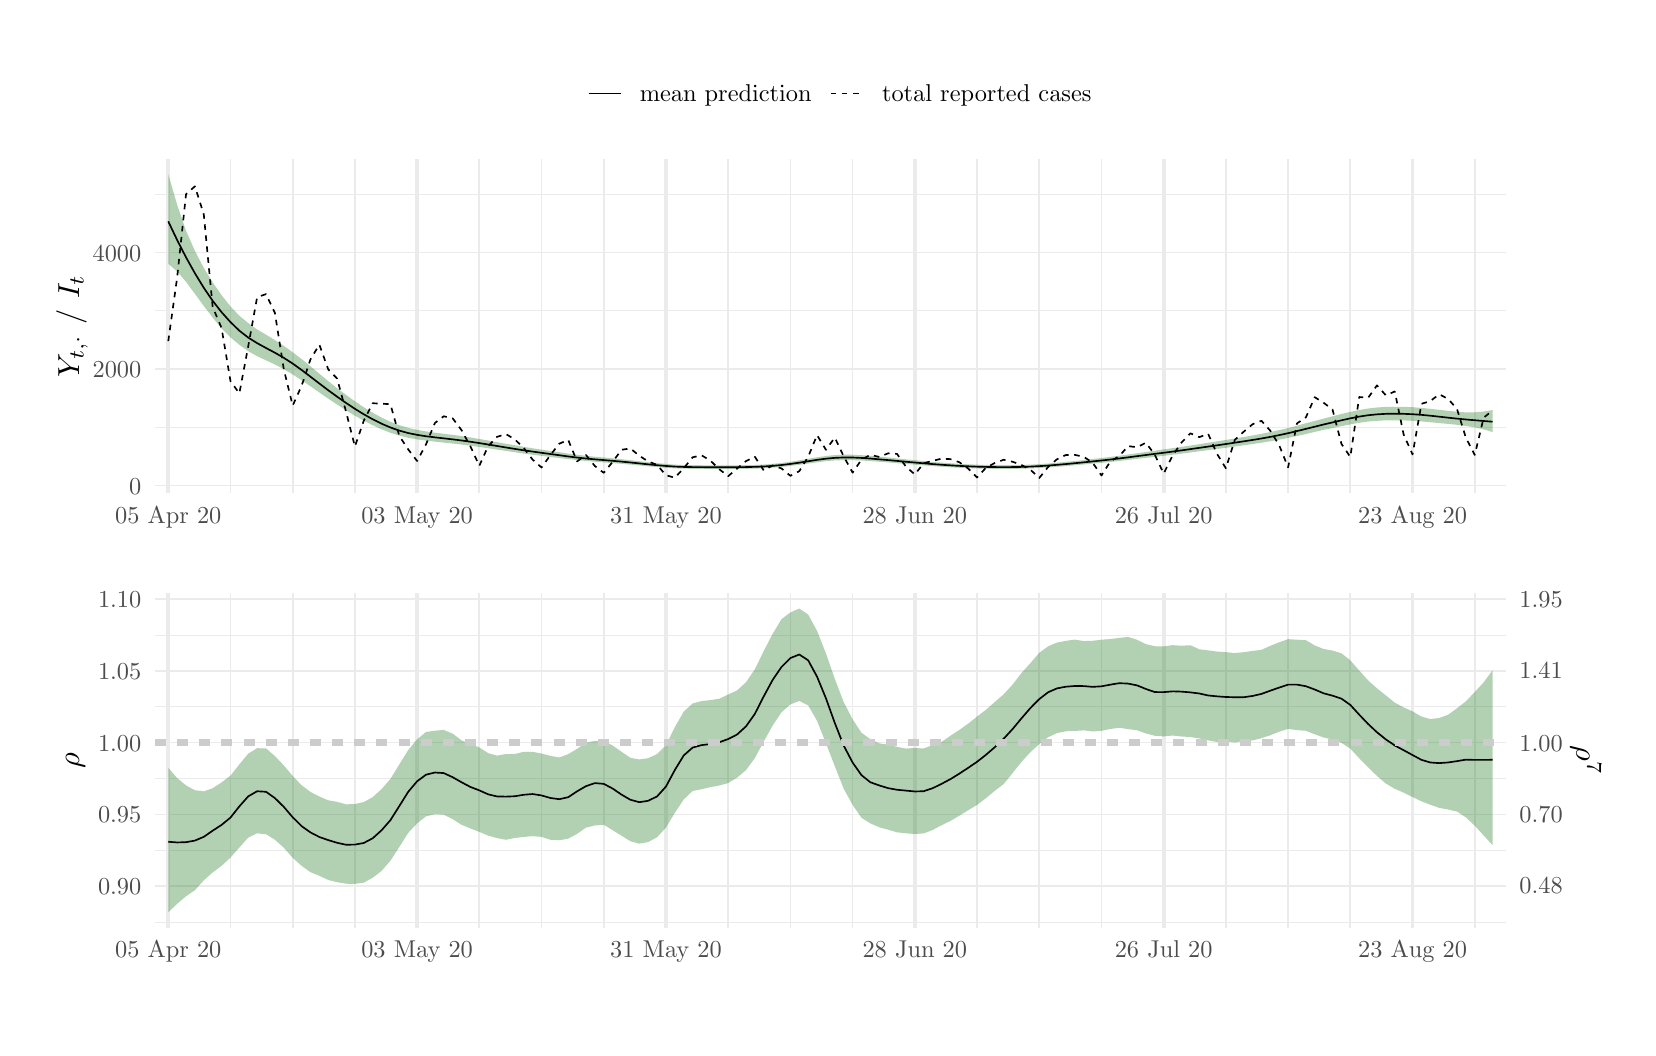
\begin{tikzpicture}[x=1pt,y=1pt]
\definecolor{fillColor}{RGB}{255,255,255}
\path[use as bounding box,fill=fillColor,fill opacity=0.00] (0,0) rectangle (578.16,361.35);
\begin{scope}
\path[clip] ( 46.01,193.13) rectangle (534.10,313.90);
\definecolor{drawColor}{gray}{0.92}

\path[draw=drawColor,line width= 0.3pt,line join=round] ( 46.01,216.91) --
	(534.10,216.91);

\path[draw=drawColor,line width= 0.3pt,line join=round] ( 46.01,259.01) --
	(534.10,259.01);

\path[draw=drawColor,line width= 0.3pt,line join=round] ( 46.01,301.11) --
	(534.10,301.11);

\path[draw=drawColor,line width= 0.6pt,line join=round] ( 73.28,193.13) --
	( 73.28,313.90);

\path[draw=drawColor,line width= 0.6pt,line join=round] ( 95.76,193.13) --
	( 95.76,313.90);

\path[draw=drawColor,line width= 0.6pt,line join=round] (118.24,193.13) --
	(118.24,313.90);

\path[draw=drawColor,line width= 0.6pt,line join=round] (163.20,193.13) --
	(163.20,313.90);

\path[draw=drawColor,line width= 0.6pt,line join=round] (185.68,193.13) --
	(185.68,313.90);

\path[draw=drawColor,line width= 0.6pt,line join=round] (208.16,193.13) --
	(208.16,313.90);

\path[draw=drawColor,line width= 0.6pt,line join=round] (253.12,193.13) --
	(253.12,313.90);

\path[draw=drawColor,line width= 0.6pt,line join=round] (275.61,193.13) --
	(275.61,313.90);

\path[draw=drawColor,line width= 0.6pt,line join=round] (298.09,193.13) --
	(298.09,313.90);

\path[draw=drawColor,line width= 0.6pt,line join=round] (343.05,193.13) --
	(343.05,313.90);

\path[draw=drawColor,line width= 0.6pt,line join=round] (365.53,193.13) --
	(365.53,313.90);

\path[draw=drawColor,line width= 0.6pt,line join=round] (388.01,193.13) --
	(388.01,313.90);

\path[draw=drawColor,line width= 0.6pt,line join=round] (432.97,193.13) --
	(432.97,313.90);

\path[draw=drawColor,line width= 0.6pt,line join=round] (455.45,193.13) --
	(455.45,313.90);

\path[draw=drawColor,line width= 0.6pt,line join=round] (477.93,193.13) --
	(477.93,313.90);

\path[draw=drawColor,line width= 0.6pt,line join=round] (522.90,193.13) --
	(522.90,313.90);

\path[draw=drawColor,line width= 0.6pt,line join=round] ( 46.01,195.87) --
	(534.10,195.87);

\path[draw=drawColor,line width= 0.6pt,line join=round] ( 46.01,237.96) --
	(534.10,237.96);

\path[draw=drawColor,line width= 0.6pt,line join=round] ( 46.01,280.06) --
	(534.10,280.06);

\path[draw=drawColor,line width= 1.4pt,line join=round] ( 50.80,193.13) --
	( 50.80,313.90);

\path[draw=drawColor,line width= 1.4pt,line join=round] (140.72,193.13) --
	(140.72,313.90);

\path[draw=drawColor,line width= 1.4pt,line join=round] (230.64,193.13) --
	(230.64,313.90);

\path[draw=drawColor,line width= 1.4pt,line join=round] (320.57,193.13) --
	(320.57,313.90);

\path[draw=drawColor,line width= 1.4pt,line join=round] (410.49,193.13) --
	(410.49,313.90);

\path[draw=drawColor,line width= 1.4pt,line join=round] (500.42,193.13) --
	(500.42,313.90);
\definecolor{fillColor}{RGB}{0,100,0}

\path[fill=fillColor,fill opacity=0.30] ( 50.80,308.41) --
	( 54.01,297.34) --
	( 57.22,287.98) --
	( 60.43,280.67) --
	( 63.64,274.53) --
	( 66.85,269.31) --
	( 70.06,264.70) --
	( 73.28,260.62) --
	( 76.49,257.24) --
	( 79.70,254.59) --
	( 82.91,252.30) --
	( 86.12,250.41) --
	( 89.33,248.47) --
	( 92.55,246.38) --
	( 95.76,244.04) --
	( 98.97,241.61) --
	(102.18,238.99) --
	(105.39,236.30) --
	(108.60,233.63) --
	(111.82,231.05) --
	(115.03,228.66) --
	(118.24,226.33) --
	(121.45,224.17) --
	(124.66,222.21) --
	(127.87,220.47) --
	(131.08,218.90) --
	(134.30,217.70) --
	(137.51,216.74) --
	(140.72,216.00) --
	(143.93,215.44) --
	(147.14,215.00) --
	(150.35,214.60) --
	(153.57,214.22) --
	(156.78,213.78) --
	(159.99,213.27) --
	(163.20,212.72) --
	(166.41,212.16) --
	(169.62,211.56) --
	(172.84,210.99) --
	(176.05,210.46) --
	(179.26,209.88) --
	(182.47,209.35) --
	(185.68,208.87) --
	(188.89,208.40) --
	(192.10,207.92) --
	(195.32,207.44) --
	(198.53,207.01) --
	(201.74,206.64) --
	(204.95,206.31) --
	(208.16,206.03) --
	(211.37,205.72) --
	(214.59,205.40) --
	(217.80,205.06) --
	(221.01,204.70) --
	(224.22,204.33) --
	(227.43,204.00) --
	(230.64,203.69) --
	(233.86,203.45) --
	(237.07,203.31) --
	(240.28,203.25) --
	(243.49,203.23) --
	(246.70,203.21) --
	(249.91,203.20) --
	(253.12,203.19) --
	(256.34,203.21) --
	(259.55,203.26) --
	(262.76,203.32) --
	(265.97,203.48) --
	(269.18,203.72) --
	(272.39,204.05) --
	(275.61,204.49) --
	(278.82,205.00) --
	(282.03,205.56) --
	(285.24,206.10) --
	(288.45,206.57) --
	(291.66,206.91) --
	(294.87,207.04) --
	(298.09,207.03) --
	(301.30,206.87) --
	(304.51,206.63) --
	(307.72,206.33) --
	(310.93,206.03) --
	(314.14,205.69) --
	(317.36,205.38) --
	(320.57,205.06) --
	(323.78,204.72) --
	(326.99,204.42) --
	(330.20,204.17) --
	(333.41,203.95) --
	(336.63,203.73) --
	(339.84,203.56) --
	(343.05,203.43) --
	(346.26,203.34) --
	(349.47,203.27) --
	(352.68,203.23) --
	(355.89,203.27) --
	(359.11,203.33) --
	(362.32,203.45) --
	(365.53,203.63) --
	(368.74,203.85) --
	(371.95,204.12) --
	(375.16,204.44) --
	(378.38,204.76) --
	(381.59,205.10) --
	(384.80,205.48) --
	(388.01,205.86) --
	(391.22,206.24) --
	(394.43,206.65) --
	(397.65,207.10) --
	(400.86,207.56) --
	(404.07,208.02) --
	(407.28,208.48) --
	(410.49,208.95) --
	(413.70,209.40) --
	(416.91,209.85) --
	(420.13,210.33) --
	(423.34,210.83) --
	(426.55,211.35) --
	(429.76,211.86) --
	(432.97,212.37) --
	(436.18,212.89) --
	(439.40,213.42) --
	(442.61,213.99) --
	(445.82,214.57) --
	(449.03,215.22) --
	(452.24,215.94) --
	(455.45,216.67) --
	(458.67,217.52) --
	(461.88,218.40) --
	(465.09,219.23) --
	(468.30,220.09) --
	(471.51,220.92) --
	(474.72,221.75) --
	(477.93,222.51) --
	(481.15,223.19) --
	(484.36,223.72) --
	(487.57,224.11) --
	(490.78,224.29) --
	(493.99,224.36) --
	(497.20,224.33) --
	(500.42,224.20) --
	(503.63,223.95) --
	(506.84,223.62) --
	(510.05,223.26) --
	(513.26,222.88) --
	(516.47,222.57) --
	(519.69,222.33) --
	(522.90,222.35) --
	(526.11,222.63) --
	(529.32,223.18) --
	(529.32,215.21) --
	(526.11,216.18) --
	(522.90,216.89) --
	(519.69,217.43) --
	(516.47,217.85) --
	(513.26,218.17) --
	(510.05,218.47) --
	(506.84,218.77) --
	(503.63,219.07) --
	(500.42,219.29) --
	(497.20,219.44) --
	(493.99,219.49) --
	(490.78,219.46) --
	(487.57,219.28) --
	(484.36,219.02) --
	(481.15,218.57) --
	(477.93,217.99) --
	(474.72,217.34) --
	(471.51,216.67) --
	(468.30,216.02) --
	(465.09,215.28) --
	(461.88,214.52) --
	(458.67,213.80) --
	(455.45,213.12) --
	(452.24,212.47) --
	(449.03,211.90) --
	(445.82,211.37) --
	(442.61,210.89) --
	(439.40,210.45) --
	(436.18,209.98) --
	(432.97,209.53) --
	(429.76,209.12) --
	(426.55,208.70) --
	(423.34,208.27) --
	(420.13,207.85) --
	(416.91,207.43) --
	(413.70,207.04) --
	(410.49,206.64) --
	(407.28,206.26) --
	(404.07,205.90) --
	(400.86,205.54) --
	(397.65,205.16) --
	(394.43,204.78) --
	(391.22,204.42) --
	(388.01,204.10) --
	(384.80,203.80) --
	(381.59,203.51) --
	(378.38,203.22) --
	(375.16,202.93) --
	(371.95,202.67) --
	(368.74,202.43) --
	(365.53,202.25) --
	(362.32,202.09) --
	(359.11,201.98) --
	(355.89,201.93) --
	(352.68,201.92) --
	(349.47,201.94) --
	(346.26,201.99) --
	(343.05,202.07) --
	(339.84,202.18) --
	(336.63,202.32) --
	(333.41,202.49) --
	(330.20,202.69) --
	(326.99,202.93) --
	(323.78,203.19) --
	(320.57,203.45) --
	(317.36,203.71) --
	(314.14,203.97) --
	(310.93,204.25) --
	(307.72,204.49) --
	(304.51,204.74) --
	(301.30,204.94) --
	(298.09,205.07) --
	(294.87,205.09) --
	(291.66,204.96) --
	(288.45,204.70) --
	(285.24,204.30) --
	(282.03,203.85) --
	(278.82,203.39) --
	(275.61,202.99) --
	(272.39,202.62) --
	(269.18,202.34) --
	(265.97,202.13) --
	(262.76,202.01) --
	(259.55,201.95) --
	(256.34,201.91) --
	(253.12,201.89) --
	(249.91,201.89) --
	(246.70,201.90) --
	(243.49,201.92) --
	(240.28,201.94) --
	(237.07,201.99) --
	(233.86,202.10) --
	(230.64,202.30) --
	(227.43,202.56) --
	(224.22,202.86) --
	(221.01,203.15) --
	(217.80,203.46) --
	(214.59,203.75) --
	(211.37,204.01) --
	(208.16,204.26) --
	(204.95,204.50) --
	(201.74,204.78) --
	(198.53,205.09) --
	(195.32,205.45) --
	(192.10,205.83) --
	(188.89,206.23) --
	(185.68,206.63) --
	(182.47,207.02) --
	(179.26,207.45) --
	(176.05,207.94) --
	(172.84,208.40) --
	(169.62,208.88) --
	(166.41,209.39) --
	(163.20,209.84) --
	(159.99,210.29) --
	(156.78,210.72) --
	(153.57,211.07) --
	(150.35,211.42) --
	(147.14,211.77) --
	(143.93,212.13) --
	(140.72,212.58) --
	(137.51,213.16) --
	(134.30,213.95) --
	(131.08,214.96) --
	(127.87,216.23) --
	(124.66,217.69) --
	(121.45,219.33) --
	(118.24,221.15) --
	(115.03,223.10) --
	(111.82,225.17) --
	(108.60,227.29) --
	(105.39,229.54) --
	(102.18,231.77) --
	( 98.97,233.95) --
	( 95.76,236.05) --
	( 92.55,237.94) --
	( 89.33,239.65) --
	( 86.12,241.14) --
	( 82.91,242.66) --
	( 79.70,244.47) --
	( 76.49,246.76) --
	( 73.28,249.43) --
	( 70.06,252.70) --
	( 66.85,256.61) --
	( 63.64,260.78) --
	( 60.43,265.18) --
	( 57.22,269.52) --
	( 54.01,273.24) --
	( 50.80,276.04) --
	cycle;

\path[] ( 50.80,308.41) --
	( 54.01,297.34) --
	( 57.22,287.98) --
	( 60.43,280.67) --
	( 63.64,274.53) --
	( 66.85,269.31) --
	( 70.06,264.70) --
	( 73.28,260.62) --
	( 76.49,257.24) --
	( 79.70,254.59) --
	( 82.91,252.30) --
	( 86.12,250.41) --
	( 89.33,248.47) --
	( 92.55,246.38) --
	( 95.76,244.04) --
	( 98.97,241.61) --
	(102.18,238.99) --
	(105.39,236.30) --
	(108.60,233.63) --
	(111.82,231.05) --
	(115.03,228.66) --
	(118.24,226.33) --
	(121.45,224.17) --
	(124.66,222.21) --
	(127.87,220.47) --
	(131.08,218.90) --
	(134.30,217.70) --
	(137.51,216.74) --
	(140.72,216.00) --
	(143.93,215.44) --
	(147.14,215.00) --
	(150.35,214.60) --
	(153.57,214.22) --
	(156.78,213.78) --
	(159.99,213.27) --
	(163.20,212.72) --
	(166.41,212.16) --
	(169.62,211.56) --
	(172.84,210.99) --
	(176.05,210.46) --
	(179.26,209.88) --
	(182.47,209.35) --
	(185.68,208.87) --
	(188.89,208.40) --
	(192.10,207.92) --
	(195.32,207.44) --
	(198.53,207.01) --
	(201.74,206.64) --
	(204.95,206.31) --
	(208.16,206.03) --
	(211.37,205.72) --
	(214.59,205.40) --
	(217.80,205.06) --
	(221.01,204.70) --
	(224.22,204.33) --
	(227.43,204.00) --
	(230.64,203.69) --
	(233.86,203.45) --
	(237.07,203.31) --
	(240.28,203.25) --
	(243.49,203.23) --
	(246.70,203.21) --
	(249.91,203.20) --
	(253.12,203.19) --
	(256.34,203.21) --
	(259.55,203.26) --
	(262.76,203.32) --
	(265.97,203.48) --
	(269.18,203.72) --
	(272.39,204.05) --
	(275.61,204.49) --
	(278.82,205.00) --
	(282.03,205.56) --
	(285.24,206.10) --
	(288.45,206.57) --
	(291.66,206.91) --
	(294.87,207.04) --
	(298.09,207.03) --
	(301.30,206.87) --
	(304.51,206.63) --
	(307.72,206.33) --
	(310.93,206.03) --
	(314.14,205.69) --
	(317.36,205.38) --
	(320.57,205.06) --
	(323.78,204.72) --
	(326.99,204.42) --
	(330.20,204.17) --
	(333.41,203.95) --
	(336.63,203.73) --
	(339.84,203.56) --
	(343.05,203.43) --
	(346.26,203.34) --
	(349.47,203.27) --
	(352.68,203.23) --
	(355.89,203.27) --
	(359.11,203.33) --
	(362.32,203.45) --
	(365.53,203.63) --
	(368.74,203.85) --
	(371.95,204.12) --
	(375.16,204.44) --
	(378.38,204.76) --
	(381.59,205.10) --
	(384.80,205.48) --
	(388.01,205.86) --
	(391.22,206.24) --
	(394.43,206.65) --
	(397.65,207.10) --
	(400.86,207.56) --
	(404.07,208.02) --
	(407.28,208.48) --
	(410.49,208.95) --
	(413.70,209.40) --
	(416.91,209.85) --
	(420.13,210.33) --
	(423.34,210.83) --
	(426.55,211.35) --
	(429.76,211.86) --
	(432.97,212.37) --
	(436.18,212.89) --
	(439.40,213.42) --
	(442.61,213.99) --
	(445.82,214.57) --
	(449.03,215.22) --
	(452.24,215.94) --
	(455.45,216.67) --
	(458.67,217.52) --
	(461.88,218.40) --
	(465.09,219.23) --
	(468.30,220.09) --
	(471.51,220.92) --
	(474.72,221.75) --
	(477.93,222.51) --
	(481.15,223.19) --
	(484.36,223.72) --
	(487.57,224.11) --
	(490.78,224.29) --
	(493.99,224.36) --
	(497.20,224.33) --
	(500.42,224.20) --
	(503.63,223.95) --
	(506.84,223.62) --
	(510.05,223.26) --
	(513.26,222.88) --
	(516.47,222.57) --
	(519.69,222.33) --
	(522.90,222.35) --
	(526.11,222.63) --
	(529.32,223.18);

\path[] (529.32,215.21) --
	(526.11,216.18) --
	(522.90,216.89) --
	(519.69,217.43) --
	(516.47,217.85) --
	(513.26,218.17) --
	(510.05,218.47) --
	(506.84,218.77) --
	(503.63,219.07) --
	(500.42,219.29) --
	(497.20,219.44) --
	(493.99,219.49) --
	(490.78,219.46) --
	(487.57,219.28) --
	(484.36,219.02) --
	(481.15,218.57) --
	(477.93,217.99) --
	(474.72,217.34) --
	(471.51,216.67) --
	(468.30,216.02) --
	(465.09,215.28) --
	(461.88,214.52) --
	(458.67,213.80) --
	(455.45,213.12) --
	(452.24,212.47) --
	(449.03,211.90) --
	(445.82,211.37) --
	(442.61,210.89) --
	(439.40,210.45) --
	(436.18,209.98) --
	(432.97,209.53) --
	(429.76,209.12) --
	(426.55,208.70) --
	(423.34,208.27) --
	(420.13,207.85) --
	(416.91,207.43) --
	(413.70,207.04) --
	(410.49,206.64) --
	(407.28,206.26) --
	(404.07,205.90) --
	(400.86,205.54) --
	(397.65,205.16) --
	(394.43,204.78) --
	(391.22,204.42) --
	(388.01,204.10) --
	(384.80,203.80) --
	(381.59,203.51) --
	(378.38,203.22) --
	(375.16,202.93) --
	(371.95,202.67) --
	(368.74,202.43) --
	(365.53,202.25) --
	(362.32,202.09) --
	(359.11,201.98) --
	(355.89,201.93) --
	(352.68,201.92) --
	(349.47,201.94) --
	(346.26,201.99) --
	(343.05,202.07) --
	(339.84,202.18) --
	(336.63,202.32) --
	(333.41,202.49) --
	(330.20,202.69) --
	(326.99,202.93) --
	(323.78,203.19) --
	(320.57,203.45) --
	(317.36,203.71) --
	(314.14,203.97) --
	(310.93,204.25) --
	(307.72,204.49) --
	(304.51,204.74) --
	(301.30,204.94) --
	(298.09,205.07) --
	(294.87,205.09) --
	(291.66,204.96) --
	(288.45,204.70) --
	(285.24,204.30) --
	(282.03,203.85) --
	(278.82,203.39) --
	(275.61,202.99) --
	(272.39,202.62) --
	(269.18,202.34) --
	(265.97,202.13) --
	(262.76,202.01) --
	(259.55,201.95) --
	(256.34,201.91) --
	(253.12,201.89) --
	(249.91,201.89) --
	(246.70,201.90) --
	(243.49,201.92) --
	(240.28,201.94) --
	(237.07,201.99) --
	(233.86,202.10) --
	(230.64,202.30) --
	(227.43,202.56) --
	(224.22,202.86) --
	(221.01,203.15) --
	(217.80,203.46) --
	(214.59,203.75) --
	(211.37,204.01) --
	(208.16,204.26) --
	(204.95,204.50) --
	(201.74,204.78) --
	(198.53,205.09) --
	(195.32,205.45) --
	(192.10,205.83) --
	(188.89,206.23) --
	(185.68,206.63) --
	(182.47,207.02) --
	(179.26,207.45) --
	(176.05,207.94) --
	(172.84,208.40) --
	(169.62,208.88) --
	(166.41,209.39) --
	(163.20,209.84) --
	(159.99,210.29) --
	(156.78,210.72) --
	(153.57,211.07) --
	(150.35,211.42) --
	(147.14,211.77) --
	(143.93,212.13) --
	(140.72,212.58) --
	(137.51,213.16) --
	(134.30,213.95) --
	(131.08,214.96) --
	(127.87,216.23) --
	(124.66,217.69) --
	(121.45,219.33) --
	(118.24,221.15) --
	(115.03,223.10) --
	(111.82,225.17) --
	(108.60,227.29) --
	(105.39,229.54) --
	(102.18,231.77) --
	( 98.97,233.95) --
	( 95.76,236.05) --
	( 92.55,237.94) --
	( 89.33,239.65) --
	( 86.12,241.14) --
	( 82.91,242.66) --
	( 79.70,244.47) --
	( 76.49,246.76) --
	( 73.28,249.43) --
	( 70.06,252.70) --
	( 66.85,256.61) --
	( 63.64,260.78) --
	( 60.43,265.18) --
	( 57.22,269.52) --
	( 54.01,273.24) --
	( 50.80,276.04);
\definecolor{drawColor}{RGB}{0,0,0}

\path[draw=drawColor,line width= 0.6pt,line join=round] ( 50.80,291.36) --
	( 54.01,284.61) --
	( 57.22,278.36) --
	( 60.43,272.60) --
	( 63.64,267.35) --
	( 66.85,262.65) --
	( 70.06,258.54) --
	( 73.28,254.95) --
	( 76.49,251.85) --
	( 79.70,249.36) --
	( 82.91,247.35) --
	( 86.12,245.60) --
	( 89.33,243.90) --
	( 92.55,242.04) --
	( 95.76,239.97) --
	( 98.97,237.67) --
	(102.18,235.23) --
	(105.39,232.77) --
	(108.60,230.34) --
	(111.82,228.00) --
	(115.03,225.75) --
	(118.24,223.62) --
	(121.45,221.65) --
	(124.66,219.85) --
	(127.87,218.25) --
	(131.08,216.88) --
	(134.30,215.74) --
	(137.51,214.86) --
	(140.72,214.21) --
	(143.93,213.71) --
	(147.14,213.31) --
	(150.35,212.95) --
	(153.57,212.58) --
	(156.78,212.18) --
	(159.99,211.73) --
	(163.20,211.24) --
	(166.41,210.72) --
	(169.62,210.19) --
	(172.84,209.65) --
	(176.05,209.13) --
	(179.26,208.63) --
	(182.47,208.17) --
	(185.68,207.72) --
	(188.89,207.29) --
	(192.10,206.85) --
	(195.32,206.41) --
	(198.53,206.01) --
	(201.74,205.66) --
	(204.95,205.37) --
	(208.16,205.10) --
	(211.37,204.83) --
	(214.59,204.54) --
	(217.80,204.23) --
	(221.01,203.90) --
	(224.22,203.56) --
	(227.43,203.25) --
	(230.64,202.97) --
	(233.86,202.75) --
	(237.07,202.62) --
	(240.28,202.56) --
	(243.49,202.54) --
	(246.70,202.52) --
	(249.91,202.52) --
	(253.12,202.52) --
	(256.34,202.53) --
	(259.55,202.57) --
	(262.76,202.65) --
	(265.97,202.78) --
	(269.18,203.00) --
	(272.39,203.31) --
	(275.61,203.70) --
	(278.82,204.16) --
	(282.03,204.67) --
	(285.24,205.18) --
	(288.45,205.60) --
	(291.66,205.90) --
	(294.87,206.04) --
	(298.09,206.02) --
	(301.30,205.87) --
	(304.51,205.65) --
	(307.72,205.37) --
	(310.93,205.09) --
	(314.14,204.80) --
	(317.36,204.50) --
	(320.57,204.21) --
	(323.78,203.93) --
	(326.99,203.65) --
	(330.20,203.41) --
	(333.41,203.19) --
	(336.63,203.00) --
	(339.84,202.85) --
	(343.05,202.72) --
	(346.26,202.63) --
	(349.47,202.57) --
	(352.68,202.55) --
	(355.89,202.57) --
	(359.11,202.63) --
	(362.32,202.74) --
	(365.53,202.91) --
	(368.74,203.12) --
	(371.95,203.38) --
	(375.16,203.66) --
	(378.38,203.96) --
	(381.59,204.28) --
	(384.80,204.61) --
	(388.01,204.95) --
	(391.22,205.30) --
	(394.43,205.68) --
	(397.65,206.09) --
	(400.86,206.51) --
	(404.07,206.93) --
	(407.28,207.34) --
	(410.49,207.74) --
	(413.70,208.16) --
	(416.91,208.60) --
	(420.13,209.05) --
	(423.34,209.51) --
	(426.55,209.97) --
	(429.76,210.43) --
	(432.97,210.90) --
	(436.18,211.38) --
	(439.40,211.87) --
	(442.61,212.37) --
	(445.82,212.90) --
	(449.03,213.48) --
	(452.24,214.12) --
	(455.45,214.81) --
	(458.67,215.58) --
	(461.88,216.37) --
	(465.09,217.17) --
	(468.30,217.96) --
	(471.51,218.71) --
	(474.72,219.46) --
	(477.93,220.18) --
	(481.15,220.81) --
	(484.36,221.30) --
	(487.57,221.62) --
	(490.78,221.81) --
	(493.99,221.86) --
	(497.20,221.81) --
	(500.42,221.67) --
	(503.63,221.44) --
	(506.84,221.13) --
	(510.05,220.78) --
	(513.26,220.42) --
	(516.47,220.08) --
	(519.69,219.77) --
	(522.90,219.49) --
	(526.11,219.22) --
	(529.32,218.96);

\path[draw=drawColor,line width= 0.6pt,dash pattern=on 2pt off 2pt ,line join=round] ( 50.80,248.07) --
	( 54.01,271.03) --
	( 57.22,301.17) --
	( 60.43,304.01) --
	( 63.64,293.87) --
	( 66.85,260.40) --
	( 70.06,252.82) --
	( 73.28,233.65) --
	( 76.49,229.19) --
	( 79.70,246.24) --
	( 82.91,263.94) --
	( 86.12,265.07) --
	( 89.33,258.30) --
	( 92.55,237.90) --
	( 95.76,224.77) --
	( 98.97,231.90) --
	(102.18,241.48) --
	(105.39,246.82) --
	(108.60,237.88) --
	(111.82,234.55) --
	(115.03,222.64) --
	(118.24,209.99) --
	(121.45,219.31) --
	(124.66,225.63) --
	(127.87,225.48) --
	(131.08,225.29) --
	(134.30,213.76) --
	(137.51,208.94) --
	(140.72,204.77) --
	(143.93,210.75) --
	(147.14,218.49) --
	(150.35,220.93) --
	(153.57,220.18) --
	(156.78,215.90) --
	(159.99,210.03) --
	(163.20,203.04) --
	(166.41,210.16) --
	(169.62,213.50) --
	(172.84,214.49) --
	(176.05,212.54) --
	(179.26,209.48) --
	(182.47,205.25) --
	(185.68,202.41) --
	(188.89,206.92) --
	(192.10,211.02) --
	(195.32,212.39) --
	(198.53,204.62) --
	(201.74,206.94) --
	(204.95,202.96) --
	(208.16,200.48) --
	(211.37,204.45) --
	(214.59,208.83) --
	(217.80,209.29) --
	(221.01,206.66) --
	(224.22,204.60) --
	(227.43,203.36) --
	(230.64,199.61) --
	(233.86,198.73) --
	(237.07,202.16) --
	(240.28,206.10) --
	(243.49,206.83) --
	(246.70,204.90) --
	(249.91,201.78) --
	(253.12,199.28) --
	(256.34,202.03) --
	(259.55,204.73) --
	(262.76,206.31) --
	(265.97,201.36) --
	(269.18,203.17) --
	(272.39,202.07) --
	(275.61,199.40) --
	(278.82,201.09) --
	(282.03,206.28) --
	(285.24,214.11) --
	(288.45,208.81) --
	(291.66,213.23) --
	(294.87,206.41) --
	(298.09,200.56) --
	(301.30,205.27) --
	(304.51,207.00) --
	(307.72,206.22) --
	(310.93,207.55) --
	(314.14,207.32) --
	(317.36,202.73) --
	(320.57,199.91) --
	(323.78,203.97) --
	(326.99,204.81) --
	(330.20,205.61) --
	(333.41,205.44) --
	(336.63,204.33) --
	(339.84,202.05) --
	(343.05,198.81) --
	(346.26,202.31) --
	(349.47,204.05) --
	(352.68,205.21) --
	(355.89,204.50) --
	(359.11,203.32) --
	(362.32,201.63) --
	(365.53,198.62) --
	(368.74,202.62) --
	(371.95,205.42) --
	(375.16,206.94) --
	(378.38,206.98) --
	(381.59,206.28) --
	(384.80,204.18) --
	(388.01,199.53) --
	(391.22,204.60) --
	(394.43,206.54) --
	(397.65,210.16) --
	(400.86,209.72) --
	(404.07,211.38) --
	(407.28,207.02) --
	(410.49,200.22) --
	(413.70,206.73) --
	(416.91,211.40) --
	(420.13,214.77) --
	(423.34,213.38) --
	(426.55,214.60) --
	(429.76,207.36) --
	(432.97,202.12) --
	(436.18,212.37) --
	(439.40,215.34) --
	(442.61,218.05) --
	(445.82,219.29) --
	(449.03,215.69) --
	(452.24,210.43) --
	(455.45,202.47) --
	(458.67,218.35) --
	(461.88,220.53) --
	(465.09,227.80) --
	(468.30,225.80) --
	(471.51,223.33) --
	(474.72,210.98) --
	(477.93,206.22) --
	(481.15,227.88) --
	(484.36,227.59) --
	(487.57,232.09) --
	(490.78,228.49) --
	(493.99,229.88) --
	(497.20,214.33) --
	(500.42,207.13) --
	(503.63,225.42) --
	(506.84,226.43) --
	(510.05,228.85) --
	(513.26,227.21) --
	(516.47,223.59) --
	(519.69,213.15) --
	(522.90,206.94) --
	(526.11,220.41) --
	(529.32,223.02);
\end{scope}
\begin{scope}
\path[clip] (  0.00,  0.00) rectangle (578.16,361.35);
\definecolor{drawColor}{gray}{0.30}

\node[text=drawColor,anchor=base east,inner sep=0pt, outer sep=0pt, scale=  0.88] at ( 41.06,192.84) {0};

\node[text=drawColor,anchor=base east,inner sep=0pt, outer sep=0pt, scale=  0.88] at ( 41.06,234.93) {2000};

\node[text=drawColor,anchor=base east,inner sep=0pt, outer sep=0pt, scale=  0.88] at ( 41.06,277.03) {4000};
\end{scope}
\begin{scope}
\path[clip] (  0.00,  0.00) rectangle (578.16,361.35);
\definecolor{drawColor}{gray}{0.30}

\node[text=drawColor,anchor=base,inner sep=0pt, outer sep=0pt, scale=  0.88] at ( 50.80,182.12) {05 Apr 20};

\node[text=drawColor,anchor=base,inner sep=0pt, outer sep=0pt, scale=  0.88] at (140.72,182.12) {03 May 20};

\node[text=drawColor,anchor=base,inner sep=0pt, outer sep=0pt, scale=  0.88] at (230.64,182.12) {31 May 20};

\node[text=drawColor,anchor=base,inner sep=0pt, outer sep=0pt, scale=  0.88] at (320.57,182.12) {28 Jun 20};

\node[text=drawColor,anchor=base,inner sep=0pt, outer sep=0pt, scale=  0.88] at (410.49,182.12) {26 Jul 20};

\node[text=drawColor,anchor=base,inner sep=0pt, outer sep=0pt, scale=  0.88] at (500.42,182.12) {23 Aug 20};
\end{scope}
\begin{scope}
\path[clip] (  0.00,  0.00) rectangle (578.16,361.35);
\definecolor{drawColor}{RGB}{0,0,0}

\node[text=drawColor,rotate= 90.00,anchor=base,inner sep=0pt, outer sep=0pt, scale=  1.10] at ( 18.58,253.51) {$Y_{t,\cdot}$ / $I_{t}$};
\end{scope}
\begin{scope}
\path[clip] ( 46.01, 36.19) rectangle (534.10,156.95);
\definecolor{drawColor}{gray}{0.92}

\path[draw=drawColor,line width= 0.3pt,line join=round] ( 46.01, 38.13) --
	(534.10, 38.13);

\path[draw=drawColor,line width= 0.3pt,line join=round] ( 46.01, 64.08) --
	(534.10, 64.08);

\path[draw=drawColor,line width= 0.3pt,line join=round] ( 46.01, 90.02) --
	(534.10, 90.02);

\path[draw=drawColor,line width= 0.3pt,line join=round] ( 46.01,115.97) --
	(534.10,115.97);

\path[draw=drawColor,line width= 0.3pt,line join=round] ( 46.01,141.92) --
	(534.10,141.92);

\path[draw=drawColor,line width= 0.6pt,line join=round] ( 73.28, 36.19) --
	( 73.28,156.95);

\path[draw=drawColor,line width= 0.6pt,line join=round] ( 95.76, 36.19) --
	( 95.76,156.95);

\path[draw=drawColor,line width= 0.6pt,line join=round] (118.24, 36.19) --
	(118.24,156.95);

\path[draw=drawColor,line width= 0.6pt,line join=round] (163.20, 36.19) --
	(163.20,156.95);

\path[draw=drawColor,line width= 0.6pt,line join=round] (185.68, 36.19) --
	(185.68,156.95);

\path[draw=drawColor,line width= 0.6pt,line join=round] (208.16, 36.19) --
	(208.16,156.95);

\path[draw=drawColor,line width= 0.6pt,line join=round] (253.12, 36.19) --
	(253.12,156.95);

\path[draw=drawColor,line width= 0.6pt,line join=round] (275.61, 36.19) --
	(275.61,156.95);

\path[draw=drawColor,line width= 0.6pt,line join=round] (298.09, 36.19) --
	(298.09,156.95);

\path[draw=drawColor,line width= 0.6pt,line join=round] (343.05, 36.19) --
	(343.05,156.95);

\path[draw=drawColor,line width= 0.6pt,line join=round] (365.53, 36.19) --
	(365.53,156.95);

\path[draw=drawColor,line width= 0.6pt,line join=round] (388.01, 36.19) --
	(388.01,156.95);

\path[draw=drawColor,line width= 0.6pt,line join=round] (432.97, 36.19) --
	(432.97,156.95);

\path[draw=drawColor,line width= 0.6pt,line join=round] (455.45, 36.19) --
	(455.45,156.95);

\path[draw=drawColor,line width= 0.6pt,line join=round] (477.93, 36.19) --
	(477.93,156.95);

\path[draw=drawColor,line width= 0.6pt,line join=round] (522.90, 36.19) --
	(522.90,156.95);

\path[draw=drawColor,line width= 0.6pt,line join=round] ( 46.01, 51.10) --
	(534.10, 51.10);

\path[draw=drawColor,line width= 0.6pt,line join=round] ( 46.01, 77.05) --
	(534.10, 77.05);

\path[draw=drawColor,line width= 0.6pt,line join=round] ( 46.01,103.00) --
	(534.10,103.00);

\path[draw=drawColor,line width= 0.6pt,line join=round] ( 46.01,128.94) --
	(534.10,128.94);

\path[draw=drawColor,line width= 0.6pt,line join=round] ( 46.01,154.89) --
	(534.10,154.89);

\path[draw=drawColor,line width= 1.4pt,line join=round] ( 50.80, 36.19) --
	( 50.80,156.95);

\path[draw=drawColor,line width= 1.4pt,line join=round] (140.72, 36.19) --
	(140.72,156.95);

\path[draw=drawColor,line width= 1.4pt,line join=round] (230.64, 36.19) --
	(230.64,156.95);

\path[draw=drawColor,line width= 1.4pt,line join=round] (320.57, 36.19) --
	(320.57,156.95);

\path[draw=drawColor,line width= 1.4pt,line join=round] (410.49, 36.19) --
	(410.49,156.95);

\path[draw=drawColor,line width= 1.4pt,line join=round] (500.42, 36.19) --
	(500.42,156.95);
\definecolor{fillColor}{RGB}{0,100,0}

\path[fill=fillColor,fill opacity=0.30] ( 50.80, 93.88) --
	( 54.01, 90.20) --
	( 57.22, 87.53) --
	( 60.43, 85.80) --
	( 63.64, 85.39) --
	( 66.85, 86.52) --
	( 70.06, 88.61) --
	( 73.28, 91.08) --
	( 76.49, 95.13) --
	( 79.70, 99.02) --
	( 82.91,100.98) --
	( 86.12,100.93) --
	( 89.33, 98.14) --
	( 92.55, 94.78) --
	( 95.76, 90.94) --
	( 98.97, 87.62) --
	(102.18, 85.19) --
	(105.39, 83.52) --
	(108.60, 82.17) --
	(111.82, 81.58) --
	(115.03, 80.70) --
	(118.24, 80.80) --
	(121.45, 81.54) --
	(124.66, 83.29) --
	(127.87, 86.21) --
	(131.08, 89.88) --
	(134.30, 95.15) --
	(137.51,100.31) --
	(140.72,104.21) --
	(143.93,106.83) --
	(147.14,107.32) --
	(150.35,107.57) --
	(153.57,106.25) --
	(156.78,103.82) --
	(159.99,102.46) --
	(163.20,101.28) --
	(166.41, 99.19) --
	(169.62, 98.30) --
	(172.84, 98.88) --
	(176.05, 98.90) --
	(179.26, 99.69) --
	(182.47, 99.69) --
	(185.68, 99.05) --
	(188.89, 98.21) --
	(192.10, 97.62) --
	(195.32, 98.84) --
	(198.53,100.75) --
	(201.74,103.00) --
	(204.95,103.62) --
	(208.16,103.63) --
	(211.37,101.94) --
	(214.59, 99.70) --
	(217.80, 97.50) --
	(221.01, 96.93) --
	(224.22, 97.38) --
	(227.43, 98.86) --
	(230.64,102.04) --
	(233.86,108.60) --
	(237.07,114.21) --
	(240.28,117.15) --
	(243.49,118.01) --
	(246.70,118.36) --
	(249.91,118.86) --
	(253.12,120.38) --
	(256.34,121.87) --
	(259.55,124.80) --
	(262.76,129.49) --
	(265.97,136.09) --
	(269.18,142.28) --
	(272.39,147.62) --
	(275.61,150.05) --
	(278.82,151.46) --
	(282.03,149.28) --
	(285.24,143.38) --
	(288.45,135.23) --
	(291.66,126.03) --
	(294.87,117.63) --
	(298.09,111.46) --
	(301.30,106.56) --
	(304.51,104.24) --
	(307.72,102.75) --
	(310.93,102.23) --
	(314.14,101.47) --
	(317.36,100.86) --
	(320.57,101.06) --
	(323.78,100.87) --
	(326.99,102.12) --
	(330.20,103.24) --
	(333.41,105.46) --
	(336.63,107.56) --
	(339.84,109.85) --
	(343.05,112.41) --
	(346.26,114.85) --
	(349.47,117.69) --
	(352.68,120.46) --
	(355.89,123.97) --
	(359.11,128.15) --
	(362.32,131.71) --
	(365.53,135.45) --
	(368.74,137.80) --
	(371.95,139.15) --
	(375.16,139.78) --
	(378.38,140.22) --
	(381.59,139.70) --
	(384.80,139.79) --
	(388.01,140.18) --
	(391.22,140.43) --
	(394.43,140.84) --
	(397.65,141.18) --
	(400.86,140.16) --
	(404.07,138.60) --
	(407.28,137.83) --
	(410.49,137.77) --
	(413.70,138.22) --
	(416.91,138.01) --
	(420.13,138.19) --
	(423.34,136.74) --
	(426.55,136.34) --
	(429.76,135.89) --
	(432.97,135.69) --
	(436.18,135.37) --
	(439.40,135.67) --
	(442.61,136.13) --
	(445.82,136.53) --
	(449.03,137.98) --
	(452.24,139.26) --
	(455.45,140.38) --
	(458.67,140.19) --
	(461.88,140.00) --
	(465.09,138.11) --
	(468.30,136.83) --
	(471.51,136.27) --
	(474.72,135.27) --
	(477.93,132.74) --
	(481.15,129.04) --
	(484.36,125.49) --
	(487.57,122.61) --
	(490.78,120.06) --
	(493.99,117.45) --
	(497.20,115.74) --
	(500.42,114.30) --
	(503.63,112.42) --
	(506.84,111.52) --
	(510.05,111.90) --
	(513.26,113.05) --
	(516.47,115.42) --
	(519.69,117.90) --
	(522.90,121.30) --
	(526.11,124.77) --
	(529.32,129.13) --
	(529.32, 65.98) --
	(526.11, 69.47) --
	(522.90, 72.99) --
	(519.69, 75.98) --
	(516.47, 78.09) --
	(513.26, 78.83) --
	(510.05, 79.43) --
	(506.84, 80.56) --
	(503.63, 81.79) --
	(500.42, 83.34) --
	(497.20, 84.94) --
	(493.99, 86.31) --
	(490.78, 88.22) --
	(487.57, 90.96) --
	(484.36, 94.10) --
	(481.15, 97.36) --
	(477.93,100.85) --
	(474.72,102.91) --
	(471.51,104.14) --
	(468.30,104.84) --
	(465.09,106.01) --
	(461.88,107.28) --
	(458.67,107.52) --
	(455.45,107.96) --
	(452.24,106.96) --
	(449.03,105.66) --
	(445.82,104.63) --
	(442.61,103.78) --
	(439.40,103.62) --
	(436.18,103.03) --
	(432.97,103.51) --
	(429.76,103.24) --
	(426.55,103.81) --
	(423.34,104.54) --
	(420.13,105.01) --
	(416.91,105.22) --
	(413.70,105.56) --
	(410.49,105.25) --
	(407.28,105.49) --
	(404.07,106.32) --
	(400.86,107.48) --
	(397.65,107.88) --
	(394.43,108.38) --
	(391.22,107.92) --
	(388.01,107.27) --
	(384.80,107.04) --
	(381.59,107.43) --
	(378.38,107.22) --
	(375.16,107.10) --
	(371.95,106.45) --
	(368.74,104.96) --
	(365.53,102.46) --
	(362.32, 99.55) --
	(359.11, 96.03) --
	(355.89, 92.00) --
	(352.68, 88.03) --
	(349.47, 85.60) --
	(346.26, 82.92) --
	(343.05, 80.50) --
	(339.84, 78.57) --
	(336.63, 76.58) --
	(333.41, 74.69) --
	(330.20, 73.14) --
	(326.99, 71.42) --
	(323.78, 70.20) --
	(320.57, 69.98) --
	(317.36, 70.22) --
	(314.14, 70.59) --
	(310.93, 71.54) --
	(307.72, 72.41) --
	(304.51, 73.83) --
	(301.30, 75.83) --
	(298.09, 80.49) --
	(294.87, 86.36) --
	(291.66, 94.49) --
	(288.45,102.77) --
	(285.24,110.88) --
	(282.03,116.47) --
	(278.82,118.08) --
	(275.61,116.81) --
	(272.39,113.98) --
	(269.18,109.13) --
	(265.97,103.40) --
	(262.76, 97.43) --
	(259.55, 93.05) --
	(256.34, 90.34) --
	(253.12, 88.39) --
	(249.91, 87.51) --
	(246.70, 86.92) --
	(243.49, 86.15) --
	(240.28, 85.53) --
	(237.07, 82.48) --
	(233.86, 77.64) --
	(230.64, 72.30) --
	(227.43, 68.81) --
	(224.22, 67.07) --
	(221.01, 66.50) --
	(217.80, 67.37) --
	(214.59, 69.37) --
	(211.37, 71.38) --
	(208.16, 73.34) --
	(204.95, 73.06) --
	(201.74, 72.29) --
	(198.53, 70.03) --
	(195.32, 68.30) --
	(192.10, 67.73) --
	(188.89, 67.90) --
	(185.68, 68.93) --
	(182.47, 69.20) --
	(179.26, 68.93) --
	(176.05, 68.57) --
	(172.84, 67.89) --
	(169.62, 68.52) --
	(166.41, 69.39) --
	(163.20, 70.76) --
	(159.99, 71.99) --
	(156.78, 73.30) --
	(153.57, 75.35) --
	(150.35, 76.95) --
	(147.14, 77.12) --
	(143.93, 76.36) --
	(140.72, 73.83) --
	(137.51, 70.41) --
	(134.30, 65.31) --
	(131.08, 60.33) --
	(127.87, 56.63) --
	(124.66, 54.20) --
	(121.45, 52.40) --
	(118.24, 51.98) --
	(115.03, 52.01) --
	(111.82, 52.58) --
	(108.60, 53.38) --
	(105.39, 54.88) --
	(102.18, 56.19) --
	( 98.97, 58.49) --
	( 95.76, 61.39) --
	( 92.55, 65.03) --
	( 89.33, 67.92) --
	( 86.12, 69.91) --
	( 82.91, 70.23) --
	( 79.70, 68.69) --
	( 76.49, 65.11) --
	( 73.28, 61.45) --
	( 70.06, 58.48) --
	( 66.85, 56.10) --
	( 63.64, 53.24) --
	( 60.43, 49.67) --
	( 57.22, 47.48) --
	( 54.01, 44.77) --
	( 50.80, 41.68) --
	cycle;

\path[] ( 50.80, 93.88) --
	( 54.01, 90.20) --
	( 57.22, 87.53) --
	( 60.43, 85.80) --
	( 63.64, 85.39) --
	( 66.85, 86.52) --
	( 70.06, 88.61) --
	( 73.28, 91.08) --
	( 76.49, 95.13) --
	( 79.70, 99.02) --
	( 82.91,100.98) --
	( 86.12,100.93) --
	( 89.33, 98.14) --
	( 92.55, 94.78) --
	( 95.76, 90.94) --
	( 98.97, 87.62) --
	(102.18, 85.19) --
	(105.39, 83.52) --
	(108.60, 82.17) --
	(111.82, 81.58) --
	(115.03, 80.70) --
	(118.24, 80.80) --
	(121.45, 81.54) --
	(124.66, 83.29) --
	(127.87, 86.21) --
	(131.08, 89.88) --
	(134.30, 95.15) --
	(137.51,100.31) --
	(140.72,104.21) --
	(143.93,106.83) --
	(147.14,107.32) --
	(150.35,107.57) --
	(153.57,106.25) --
	(156.78,103.82) --
	(159.99,102.46) --
	(163.20,101.28) --
	(166.41, 99.19) --
	(169.62, 98.30) --
	(172.84, 98.88) --
	(176.05, 98.90) --
	(179.26, 99.69) --
	(182.47, 99.69) --
	(185.68, 99.05) --
	(188.89, 98.21) --
	(192.10, 97.62) --
	(195.32, 98.84) --
	(198.53,100.75) --
	(201.74,103.00) --
	(204.95,103.62) --
	(208.16,103.63) --
	(211.37,101.94) --
	(214.59, 99.70) --
	(217.80, 97.50) --
	(221.01, 96.93) --
	(224.22, 97.38) --
	(227.43, 98.86) --
	(230.64,102.04) --
	(233.86,108.60) --
	(237.07,114.21) --
	(240.28,117.15) --
	(243.49,118.01) --
	(246.70,118.36) --
	(249.91,118.86) --
	(253.12,120.38) --
	(256.34,121.87) --
	(259.55,124.80) --
	(262.76,129.49) --
	(265.97,136.09) --
	(269.18,142.28) --
	(272.39,147.62) --
	(275.61,150.05) --
	(278.82,151.46) --
	(282.03,149.28) --
	(285.24,143.38) --
	(288.45,135.23) --
	(291.66,126.03) --
	(294.87,117.63) --
	(298.09,111.46) --
	(301.30,106.56) --
	(304.51,104.24) --
	(307.72,102.75) --
	(310.93,102.23) --
	(314.14,101.47) --
	(317.36,100.86) --
	(320.57,101.06) --
	(323.78,100.87) --
	(326.99,102.12) --
	(330.20,103.24) --
	(333.41,105.46) --
	(336.63,107.56) --
	(339.84,109.85) --
	(343.05,112.41) --
	(346.26,114.85) --
	(349.47,117.69) --
	(352.68,120.46) --
	(355.89,123.97) --
	(359.11,128.15) --
	(362.32,131.71) --
	(365.53,135.45) --
	(368.74,137.80) --
	(371.95,139.15) --
	(375.16,139.78) --
	(378.38,140.22) --
	(381.59,139.70) --
	(384.80,139.79) --
	(388.01,140.18) --
	(391.22,140.43) --
	(394.43,140.84) --
	(397.65,141.18) --
	(400.86,140.16) --
	(404.07,138.60) --
	(407.28,137.83) --
	(410.49,137.77) --
	(413.70,138.22) --
	(416.91,138.01) --
	(420.13,138.19) --
	(423.34,136.74) --
	(426.55,136.34) --
	(429.76,135.89) --
	(432.97,135.69) --
	(436.18,135.37) --
	(439.40,135.67) --
	(442.61,136.13) --
	(445.82,136.53) --
	(449.03,137.98) --
	(452.24,139.26) --
	(455.45,140.38) --
	(458.67,140.19) --
	(461.88,140.00) --
	(465.09,138.11) --
	(468.30,136.83) --
	(471.51,136.27) --
	(474.72,135.27) --
	(477.93,132.74) --
	(481.15,129.04) --
	(484.36,125.49) --
	(487.57,122.61) --
	(490.78,120.06) --
	(493.99,117.45) --
	(497.20,115.74) --
	(500.42,114.30) --
	(503.63,112.42) --
	(506.84,111.52) --
	(510.05,111.90) --
	(513.26,113.05) --
	(516.47,115.42) --
	(519.69,117.90) --
	(522.90,121.30) --
	(526.11,124.77) --
	(529.32,129.13);

\path[] (529.32, 65.98) --
	(526.11, 69.47) --
	(522.90, 72.99) --
	(519.69, 75.98) --
	(516.47, 78.09) --
	(513.26, 78.83) --
	(510.05, 79.43) --
	(506.84, 80.56) --
	(503.63, 81.79) --
	(500.42, 83.34) --
	(497.20, 84.94) --
	(493.99, 86.31) --
	(490.78, 88.22) --
	(487.57, 90.96) --
	(484.36, 94.10) --
	(481.15, 97.36) --
	(477.93,100.85) --
	(474.72,102.91) --
	(471.51,104.14) --
	(468.30,104.84) --
	(465.09,106.01) --
	(461.88,107.28) --
	(458.67,107.52) --
	(455.45,107.96) --
	(452.24,106.96) --
	(449.03,105.66) --
	(445.82,104.63) --
	(442.61,103.78) --
	(439.40,103.62) --
	(436.18,103.03) --
	(432.97,103.51) --
	(429.76,103.24) --
	(426.55,103.81) --
	(423.34,104.54) --
	(420.13,105.01) --
	(416.91,105.22) --
	(413.70,105.56) --
	(410.49,105.25) --
	(407.28,105.49) --
	(404.07,106.32) --
	(400.86,107.48) --
	(397.65,107.88) --
	(394.43,108.38) --
	(391.22,107.92) --
	(388.01,107.27) --
	(384.80,107.04) --
	(381.59,107.43) --
	(378.38,107.22) --
	(375.16,107.10) --
	(371.95,106.45) --
	(368.74,104.96) --
	(365.53,102.46) --
	(362.32, 99.55) --
	(359.11, 96.03) --
	(355.89, 92.00) --
	(352.68, 88.03) --
	(349.47, 85.60) --
	(346.26, 82.92) --
	(343.05, 80.50) --
	(339.84, 78.57) --
	(336.63, 76.58) --
	(333.41, 74.69) --
	(330.20, 73.14) --
	(326.99, 71.42) --
	(323.78, 70.20) --
	(320.57, 69.98) --
	(317.36, 70.22) --
	(314.14, 70.59) --
	(310.93, 71.54) --
	(307.72, 72.41) --
	(304.51, 73.83) --
	(301.30, 75.83) --
	(298.09, 80.49) --
	(294.87, 86.36) --
	(291.66, 94.49) --
	(288.45,102.77) --
	(285.24,110.88) --
	(282.03,116.47) --
	(278.82,118.08) --
	(275.61,116.81) --
	(272.39,113.98) --
	(269.18,109.13) --
	(265.97,103.40) --
	(262.76, 97.43) --
	(259.55, 93.05) --
	(256.34, 90.34) --
	(253.12, 88.39) --
	(249.91, 87.51) --
	(246.70, 86.92) --
	(243.49, 86.15) --
	(240.28, 85.53) --
	(237.07, 82.48) --
	(233.86, 77.64) --
	(230.64, 72.30) --
	(227.43, 68.81) --
	(224.22, 67.07) --
	(221.01, 66.50) --
	(217.80, 67.37) --
	(214.59, 69.37) --
	(211.37, 71.38) --
	(208.16, 73.34) --
	(204.95, 73.06) --
	(201.74, 72.29) --
	(198.53, 70.03) --
	(195.32, 68.30) --
	(192.10, 67.73) --
	(188.89, 67.90) --
	(185.68, 68.93) --
	(182.47, 69.20) --
	(179.26, 68.93) --
	(176.05, 68.57) --
	(172.84, 67.89) --
	(169.62, 68.52) --
	(166.41, 69.39) --
	(163.20, 70.76) --
	(159.99, 71.99) --
	(156.78, 73.30) --
	(153.57, 75.35) --
	(150.35, 76.95) --
	(147.14, 77.12) --
	(143.93, 76.36) --
	(140.72, 73.83) --
	(137.51, 70.41) --
	(134.30, 65.31) --
	(131.08, 60.33) --
	(127.87, 56.63) --
	(124.66, 54.20) --
	(121.45, 52.40) --
	(118.24, 51.98) --
	(115.03, 52.01) --
	(111.82, 52.58) --
	(108.60, 53.38) --
	(105.39, 54.88) --
	(102.18, 56.19) --
	( 98.97, 58.49) --
	( 95.76, 61.39) --
	( 92.55, 65.03) --
	( 89.33, 67.92) --
	( 86.12, 69.91) --
	( 82.91, 70.23) --
	( 79.70, 68.69) --
	( 76.49, 65.11) --
	( 73.28, 61.45) --
	( 70.06, 58.48) --
	( 66.85, 56.10) --
	( 63.64, 53.24) --
	( 60.43, 49.67) --
	( 57.22, 47.48) --
	( 54.01, 44.77) --
	( 50.80, 41.68);
\definecolor{drawColor}{RGB}{0,0,0}

\path[draw=drawColor,line width= 0.6pt,line join=round] ( 50.80, 67.18) --
	( 54.01, 66.93) --
	( 57.22, 67.03) --
	( 60.43, 67.60) --
	( 63.64, 68.96) --
	( 66.85, 71.18) --
	( 70.06, 73.27) --
	( 73.28, 75.91) --
	( 76.49, 79.97) --
	( 79.70, 83.58) --
	( 82.91, 85.43) --
	( 86.12, 85.24) --
	( 89.33, 82.96) --
	( 92.55, 79.79) --
	( 95.76, 76.03) --
	( 98.97, 72.83) --
	(102.18, 70.56) --
	(105.39, 68.90) --
	(108.60, 67.78) --
	(111.82, 66.80) --
	(115.03, 66.10) --
	(118.24, 66.15) --
	(121.45, 66.74) --
	(124.66, 68.43) --
	(127.87, 71.32) --
	(131.08, 74.99) --
	(134.30, 80.09) --
	(137.51, 85.23) --
	(140.72, 89.03) --
	(143.93, 91.40) --
	(147.14, 92.20) --
	(150.35, 91.99) --
	(153.57, 90.50) --
	(156.78, 88.68) --
	(159.99, 86.98) --
	(163.20, 85.75) --
	(166.41, 84.31) --
	(169.62, 83.55) --
	(172.84, 83.49) --
	(176.05, 83.62) --
	(179.26, 84.16) --
	(182.47, 84.42) --
	(185.68, 83.92) --
	(188.89, 82.99) --
	(192.10, 82.56) --
	(195.32, 83.28) --
	(198.53, 85.40) --
	(201.74, 87.27) --
	(204.95, 88.37) --
	(208.16, 88.11) --
	(211.37, 86.41) --
	(214.59, 84.21) --
	(217.80, 82.35) --
	(221.01, 81.48) --
	(224.22, 81.98) --
	(227.43, 83.56) --
	(230.64, 87.12) --
	(233.86, 93.12) --
	(237.07, 98.38) --
	(240.28,101.20) --
	(243.49,102.10) --
	(246.70,102.47) --
	(249.91,103.14) --
	(253.12,104.29) --
	(256.34,105.93) --
	(259.55,108.86) --
	(262.76,113.38) --
	(265.97,119.70) --
	(269.18,125.64) --
	(272.39,130.35) --
	(275.61,133.55) --
	(278.82,134.85) --
	(282.03,132.74) --
	(285.24,126.82) --
	(288.45,119.02) --
	(291.66,110.07) --
	(294.87,101.93) --
	(298.09, 95.79) --
	(301.30, 91.24) --
	(304.51, 88.67) --
	(307.72, 87.53) --
	(310.93, 86.55) --
	(314.14, 85.97) --
	(317.36, 85.66) --
	(320.57, 85.35) --
	(323.78, 85.44) --
	(326.99, 86.52) --
	(330.20, 88.09) --
	(333.41, 89.79) --
	(336.63, 91.78) --
	(339.84, 93.89) --
	(343.05, 96.07) --
	(346.26, 98.59) --
	(349.47,101.36) --
	(352.68,104.42) --
	(355.89,107.90) --
	(359.11,111.77) --
	(362.32,115.49) --
	(365.53,118.72) --
	(368.74,121.21) --
	(371.95,122.60) --
	(375.16,123.21) --
	(378.38,123.46) --
	(381.59,123.43) --
	(384.80,123.15) --
	(388.01,123.34) --
	(391.22,123.95) --
	(394.43,124.48) --
	(397.65,124.33) --
	(400.86,123.69) --
	(404.07,122.38) --
	(407.28,121.27) --
	(410.49,121.25) --
	(413.70,121.53) --
	(416.91,121.43) --
	(420.13,121.16) --
	(423.34,120.76) --
	(426.55,120.04) --
	(429.76,119.72) --
	(432.97,119.49) --
	(436.18,119.40) --
	(439.40,119.40) --
	(442.61,119.86) --
	(445.82,120.60) --
	(449.03,121.77) --
	(452.24,122.90) --
	(455.45,123.96) --
	(458.67,123.96) --
	(461.88,123.38) --
	(465.09,122.18) --
	(468.30,120.81) --
	(471.51,119.96) --
	(474.72,118.90) --
	(477.93,116.62) --
	(481.15,113.10) --
	(484.36,109.74) --
	(487.57,106.73) --
	(490.78,104.16) --
	(493.99,101.98) --
	(497.20,100.26) --
	(500.42, 98.51) --
	(503.63, 96.78) --
	(506.84, 95.82) --
	(510.05, 95.60) --
	(513.26, 95.83) --
	(516.47, 96.31) --
	(519.69, 96.85) --
	(522.90, 96.76) --
	(526.11, 96.77) --
	(529.32, 96.79);
\definecolor{drawColor}{gray}{0.80}

\path[draw=drawColor,line width= 2.3pt,dash pattern=on 4pt off 4pt ,line join=round] ( 46.01,103.00) -- (534.10,103.00);
\end{scope}
\begin{scope}
\path[clip] (  0.00,  0.00) rectangle (578.16,361.35);
\definecolor{drawColor}{gray}{0.30}

\node[text=drawColor,anchor=base east,inner sep=0pt, outer sep=0pt, scale=  0.88] at ( 41.06, 48.07) {0.90};

\node[text=drawColor,anchor=base east,inner sep=0pt, outer sep=0pt, scale=  0.88] at ( 41.06, 74.02) {0.95};

\node[text=drawColor,anchor=base east,inner sep=0pt, outer sep=0pt, scale=  0.88] at ( 41.06, 99.97) {1.00};

\node[text=drawColor,anchor=base east,inner sep=0pt, outer sep=0pt, scale=  0.88] at ( 41.06,125.91) {1.05};

\node[text=drawColor,anchor=base east,inner sep=0pt, outer sep=0pt, scale=  0.88] at ( 41.06,151.86) {1.10};
\end{scope}
\begin{scope}
\path[clip] (  0.00,  0.00) rectangle (578.16,361.35);
\definecolor{drawColor}{gray}{0.30}

\node[text=drawColor,anchor=base west,inner sep=0pt, outer sep=0pt, scale=  0.88] at (539.05, 48.31) {0.48};

\node[text=drawColor,anchor=base west,inner sep=0pt, outer sep=0pt, scale=  0.88] at (539.05, 74.19) {0.70};

\node[text=drawColor,anchor=base west,inner sep=0pt, outer sep=0pt, scale=  0.88] at (539.05, 99.97) {1.00};

\node[text=drawColor,anchor=base west,inner sep=0pt, outer sep=0pt, scale=  0.88] at (539.05,126.07) {1.41};

\node[text=drawColor,anchor=base west,inner sep=0pt, outer sep=0pt, scale=  0.88] at (539.05,151.91) {1.95};
\end{scope}
\begin{scope}
\path[clip] (  0.00,  0.00) rectangle (578.16,361.35);
\definecolor{drawColor}{gray}{0.30}

\node[text=drawColor,anchor=base,inner sep=0pt, outer sep=0pt, scale=  0.88] at ( 50.80, 25.18) {05 Apr 20};

\node[text=drawColor,anchor=base,inner sep=0pt, outer sep=0pt, scale=  0.88] at (140.72, 25.18) {03 May 20};

\node[text=drawColor,anchor=base,inner sep=0pt, outer sep=0pt, scale=  0.88] at (230.64, 25.18) {31 May 20};

\node[text=drawColor,anchor=base,inner sep=0pt, outer sep=0pt, scale=  0.88] at (320.57, 25.18) {28 Jun 20};

\node[text=drawColor,anchor=base,inner sep=0pt, outer sep=0pt, scale=  0.88] at (410.49, 25.18) {26 Jul 20};

\node[text=drawColor,anchor=base,inner sep=0pt, outer sep=0pt, scale=  0.88] at (500.42, 25.18) {23 Aug 20};
\end{scope}
\begin{scope}
\path[clip] (  0.00,  0.00) rectangle (578.16,361.35);
\definecolor{drawColor}{RGB}{0,0,0}

\node[text=drawColor,rotate= 90.00,anchor=base,inner sep=0pt, outer sep=0pt, scale=  1.10] at ( 18.58, 96.57) {$\rho$};
\end{scope}
\begin{scope}
\path[clip] (  0.00,  0.00) rectangle (578.16,361.35);
\definecolor{drawColor}{RGB}{0,0,0}

\node[text=drawColor,rotate=-90.00,anchor=base,inner sep=0pt, outer sep=0pt, scale=  1.10] at (559.58, 96.57) {$\rho^7$};
\end{scope}
\begin{scope}
\path[clip] (  0.00,  0.00) rectangle (578.16,361.35);
\definecolor{drawColor}{RGB}{0,0,0}

\path[draw=drawColor,line width= 0.6pt,line join=round] (202.67,337.62) -- (214.23,337.62);
\end{scope}
\begin{scope}
\path[clip] (  0.00,  0.00) rectangle (578.16,361.35);
\definecolor{drawColor}{RGB}{0,0,0}

\path[draw=drawColor,line width= 0.6pt,dash pattern=on 2pt off 2pt ,line join=round] (290.22,337.62) -- (301.78,337.62);
\end{scope}
\begin{scope}
\path[clip] (  0.00,  0.00) rectangle (578.16,361.35);
\definecolor{drawColor}{RGB}{0,0,0}

\node[text=drawColor,anchor=base west,inner sep=0pt, outer sep=0pt, scale=  0.88] at (221.18,334.59) {mean prediction};
\end{scope}
\begin{scope}
\path[clip] (  0.00,  0.00) rectangle (578.16,361.35);
\definecolor{drawColor}{RGB}{0,0,0}

\node[text=drawColor,anchor=base west,inner sep=0pt, outer sep=0pt, scale=  0.88] at (308.73,334.59) {total reported cases};
\end{scope}
\end{tikzpicture}
%
    }
    \caption{Monte-Carlo estimates of mean and $95\%$ prediction intervals for smoothed incidences $I$ and daily growth factors $\rho$. The total reported cases with delay at most $4$ days,  $Y_{t}$, is shown as a dotted line. The secondary axis for the daily growth factor $\rho$ indicates the corresponding weekly growth factors $\rho^{7}$ which are easier to interpret. The gray dashed line indicates the threshold for growth $\rho = 1$.}
    \label{fig:showcase_prediction_intervals_I_rho}
\end{figure}

We show MC-estimates of the mean and $95\%$ prediction intervals of the conditional distribution of $I$ and $\rho$ (\Cref{fig:showcase_prediction_intervals_I_rho}) as well as $W,M$ and $p$ (\Cref{fig:showcase_prediction_intervals}), based on the procedure described in \Cref{subsec:inference}. For $I$ we additionally show the total number of reported cases with delay at most $4$ days, $Y_{t} = Y_{t, 1} + \dots + Y_{t, 4}$, as a sanity check. Indeed, $I$ is a smoothed version of $Y$, which removes weekday-effects and small discrepancies in reporting, as these effects are captured by the $W$ and $M$ terms.

For the daily growth factor $\rho$ we additionally display the corresponding weekly growth factors $\rho^{7}$ on the secondary axis. We see that uncertainty for $\rho$ is roughly constant over time, except close to the beginning and end of the time period considered here. We see that until June 2020 $\rho$ is below $1$, followed by a short skip above $1$ during the local outbreak highlighted in \Cref{fig:cases_germany} and a return to $\rho < 1$ until beginning of July 2020. We will deal with this sudden increase and the following decrease more extensively in the following section. From the middle of July 2020 to the middle of August 2020, $\rho$ is consistently above $1$, with a slight dip at the end of August, before rising above $1$ again. That cases are, or will be, rising exponentially is easier to infer from $\rho$ compared to $I$, as $\rho$, or $\rho^7$ for that matter, directly quantifies the increase in cases. Thus, this sustained period of exponential growth could have been a warning sign to policymakers of the buildup of infections in the population, which only became noticeable in the cases starting in October 2020. 

\begin{figure}
    \resizebox{\textwidth}{!}{%
        % Created by tikzDevice version 0.12.6 on 2024-09-19 10:26:55
% !TEX encoding = UTF-8 Unicode
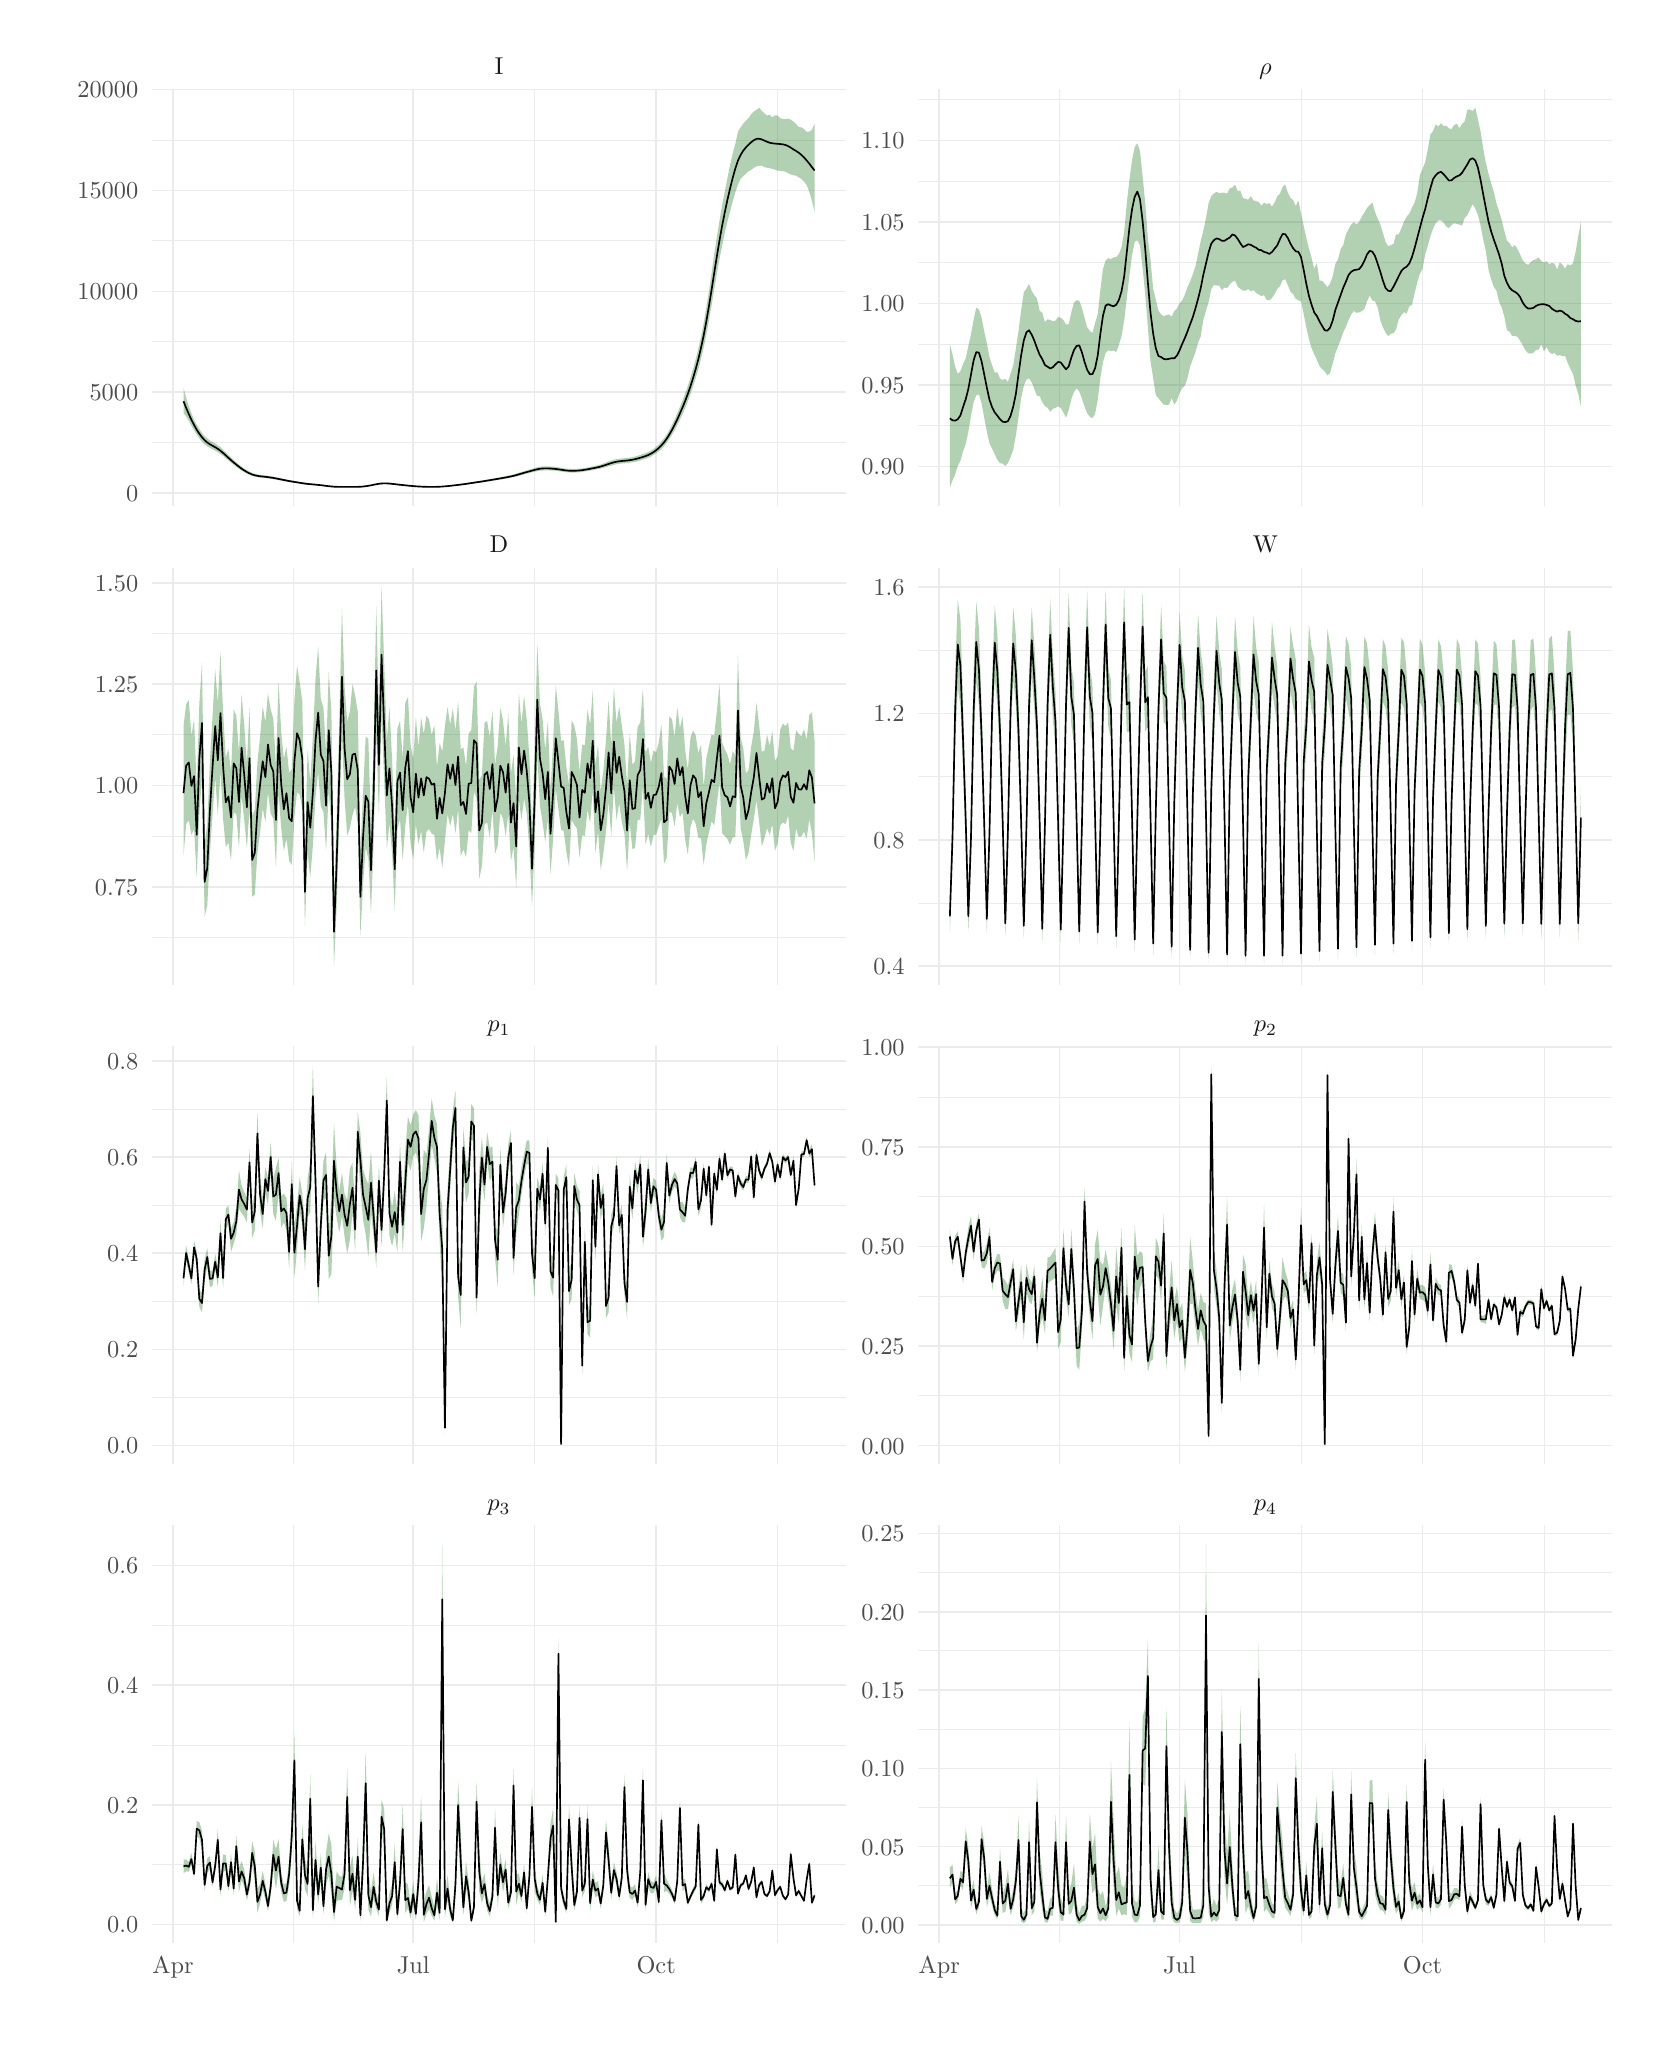
\begin{tikzpicture}[x=1pt,y=1pt]
\definecolor{fillColor}{RGB}{255,255,255}
\path[use as bounding box,fill=fillColor,fill opacity=0.00] (0,0) rectangle (578.16,722.70);
\begin{scope}
\path[clip] ( 44.91,549.70) rectangle (295.74,700.63);
\definecolor{drawColor}{gray}{0.92}

\path[draw=drawColor,line width= 0.3pt,line join=round] ( 44.91,572.69) --
	(295.74,572.69);

\path[draw=drawColor,line width= 0.3pt,line join=round] ( 44.91,609.17) --
	(295.74,609.17);

\path[draw=drawColor,line width= 0.3pt,line join=round] ( 44.91,645.65) --
	(295.74,645.65);

\path[draw=drawColor,line width= 0.3pt,line join=round] ( 44.91,682.13) --
	(295.74,682.13);

\path[draw=drawColor,line width= 0.3pt,line join=round] ( 95.91,549.70) --
	( 95.91,700.63);

\path[draw=drawColor,line width= 0.3pt,line join=round] (183.20,549.70) --
	(183.20,700.63);

\path[draw=drawColor,line width= 0.3pt,line join=round] (270.98,549.70) --
	(270.98,700.63);

\path[draw=drawColor,line width= 0.6pt,line join=round] ( 44.91,554.45) --
	(295.74,554.45);

\path[draw=drawColor,line width= 0.6pt,line join=round] ( 44.91,590.93) --
	(295.74,590.93);

\path[draw=drawColor,line width= 0.6pt,line join=round] ( 44.91,627.41) --
	(295.74,627.41);

\path[draw=drawColor,line width= 0.6pt,line join=round] ( 44.91,663.89) --
	(295.74,663.89);

\path[draw=drawColor,line width= 0.6pt,line join=round] ( 44.91,700.37) --
	(295.74,700.37);

\path[draw=drawColor,line width= 0.6pt,line join=round] ( 52.49,549.70) --
	( 52.49,700.63);

\path[draw=drawColor,line width= 0.6pt,line join=round] (139.32,549.70) --
	(139.32,700.63);

\path[draw=drawColor,line width= 0.6pt,line join=round] (227.09,549.70) --
	(227.09,700.63);
\definecolor{fillColor}{RGB}{0,100,0}

\path[fill=fillColor,fill opacity=0.30] ( 56.31,592.55) --
	( 57.26,588.96) --
	( 58.22,585.92) --
	( 59.17,583.32) --
	( 60.13,581.07) --
	( 61.08,579.25) --
	( 62.03,577.65) --
	( 62.99,576.24) --
	( 63.94,575.09) --
	( 64.90,574.27) --
	( 65.85,573.49) --
	( 66.81,572.93) --
	( 67.76,572.48) --
	( 68.71,571.83) --
	( 69.67,571.09) --
	( 70.62,570.18) --
	( 71.58,569.27) --
	( 72.53,568.28) --
	( 73.48,567.40) --
	( 74.44,566.45) --
	( 75.39,565.60) --
	( 76.35,564.81) --
	( 77.30,564.08) --
	( 78.25,563.38) --
	( 79.21,562.79) --
	( 80.16,562.25) --
	( 81.12,561.81) --
	( 82.07,561.50) --
	( 83.02,561.27) --
	( 83.98,561.11) --
	( 84.93,561.01) --
	( 85.89,560.89) --
	( 86.84,560.76) --
	( 87.80,560.61) --
	( 88.75,560.46) --
	( 89.70,560.24) --
	( 90.66,560.05) --
	( 91.61,559.83) --
	( 92.57,559.62) --
	( 93.52,559.43) --
	( 94.47,559.23) --
	( 95.43,559.06) --
	( 96.38,558.91) --
	( 97.34,558.74) --
	( 98.29,558.58) --
	( 99.24,558.42) --
	(100.20,558.24) --
	(101.15,558.13) --
	(102.11,558.04) --
	(103.06,557.92) --
	(104.01,557.83) --
	(104.97,557.73) --
	(105.92,557.61) --
	(106.88,557.48) --
	(107.83,557.37) --
	(108.79,557.24) --
	(109.74,557.13) --
	(110.69,557.05) --
	(111.65,556.99) --
	(112.60,556.97) --
	(113.56,556.96) --
	(114.51,556.96) --
	(115.46,556.96) --
	(116.42,556.96) --
	(117.37,556.96) --
	(118.33,556.97) --
	(119.28,556.99) --
	(120.23,557.02) --
	(121.19,557.11) --
	(122.14,557.22) --
	(123.10,557.38) --
	(124.05,557.56) --
	(125.00,557.77) --
	(125.96,557.99) --
	(126.91,558.16) --
	(127.87,558.29) --
	(128.82,558.31) --
	(129.78,558.29) --
	(130.73,558.24) --
	(131.68,558.15) --
	(132.64,558.04) --
	(133.59,557.91) --
	(134.55,557.80) --
	(135.50,557.68) --
	(136.45,557.57) --
	(137.41,557.45) --
	(138.36,557.34) --
	(139.32,557.26) --
	(140.27,557.18) --
	(141.22,557.10) --
	(142.18,557.05) --
	(143.13,557.00) --
	(144.09,556.97) --
	(145.04,556.96) --
	(145.99,556.95) --
	(146.95,556.95) --
	(147.90,556.98) --
	(148.86,557.02) --
	(149.81,557.08) --
	(150.77,557.17) --
	(151.72,557.26) --
	(152.67,557.37) --
	(153.63,557.47) --
	(154.58,557.59) --
	(155.54,557.72) --
	(156.49,557.84) --
	(157.44,557.99) --
	(158.40,558.13) --
	(159.35,558.27) --
	(160.31,558.44) --
	(161.26,558.59) --
	(162.21,558.74) --
	(163.17,558.92) --
	(164.12,559.08) --
	(165.08,559.24) --
	(166.03,559.37) --
	(166.98,559.54) --
	(167.94,559.71) --
	(168.89,559.89) --
	(169.85,560.08) --
	(170.80,560.25) --
	(171.76,560.45) --
	(172.71,560.65) --
	(173.66,560.84) --
	(174.62,561.06) --
	(175.57,561.30) --
	(176.53,561.60) --
	(177.48,561.86) --
	(178.43,562.14) --
	(179.39,562.39) --
	(180.34,562.70) --
	(181.30,563.00) --
	(182.25,563.27) --
	(183.20,563.58) --
	(184.16,563.85) --
	(185.11,564.00) --
	(186.07,564.13) --
	(187.02,564.18) --
	(187.97,564.15) --
	(188.93,564.11) --
	(189.88,564.05) --
	(190.84,563.96) --
	(191.79,563.81) --
	(192.75,563.65) --
	(193.70,563.48) --
	(194.65,563.32) --
	(195.61,563.28) --
	(196.56,563.21) --
	(197.52,563.20) --
	(198.47,563.24) --
	(199.42,563.32) --
	(200.38,563.44) --
	(201.33,563.59) --
	(202.29,563.78) --
	(203.24,563.96) --
	(204.19,564.18) --
	(205.15,564.38) --
	(206.10,564.57) --
	(207.06,564.83) --
	(208.01,565.19) --
	(208.96,565.57) --
	(209.92,565.97) --
	(210.87,566.23) --
	(211.83,566.55) --
	(212.78,566.77) --
	(213.74,566.92) --
	(214.69,567.02) --
	(215.64,567.11) --
	(216.60,567.26) --
	(217.55,567.31) --
	(218.51,567.49) --
	(219.46,567.72) --
	(220.41,567.99) --
	(221.37,568.28) --
	(222.32,568.65) --
	(223.28,568.95) --
	(224.23,569.36) --
	(225.18,569.86) --
	(226.14,570.42) --
	(227.09,571.14) --
	(228.05,572.08) --
	(229.00,573.13) --
	(229.95,574.26) --
	(230.91,575.67) --
	(231.86,577.29) --
	(232.82,579.17) --
	(233.77,581.16) --
	(234.73,583.35) --
	(235.68,585.62) --
	(236.63,587.99) --
	(237.59,590.56) --
	(238.54,593.20) --
	(239.50,596.31) --
	(240.45,599.45) --
	(241.40,602.94) --
	(242.36,606.78) --
	(243.31,611.02) --
	(244.27,615.96) --
	(245.22,621.51) --
	(246.17,627.45) --
	(247.13,633.89) --
	(248.08,640.90) --
	(249.04,647.06) --
	(249.99,652.97) --
	(250.94,658.61) --
	(251.90,663.44) --
	(252.85,668.40) --
	(253.81,672.98) --
	(254.76,677.21) --
	(255.72,680.76) --
	(256.67,685.12) --
	(257.62,686.62) --
	(258.58,688.04) --
	(259.53,689.08) --
	(260.49,690.04) --
	(261.44,691.42) --
	(262.39,692.38) --
	(263.35,693.00) --
	(264.30,693.77) --
	(265.26,692.62) --
	(266.21,691.77) --
	(267.16,690.96) --
	(268.12,691.18) --
	(269.07,690.31) --
	(270.03,691.04) --
	(270.98,690.94) --
	(271.93,690.01) --
	(272.89,689.67) --
	(273.84,689.61) --
	(274.80,689.86) --
	(275.75,689.39) --
	(276.71,688.78) --
	(277.66,687.88) --
	(278.61,686.74) --
	(279.57,686.69) --
	(280.52,686.05) --
	(281.48,685.07) --
	(282.43,685.10) --
	(283.38,685.80) --
	(284.34,688.02) --
	(284.34,656.02) --
	(283.38,660.18) --
	(282.43,663.37) --
	(281.48,665.86) --
	(280.52,667.07) --
	(279.57,668.08) --
	(278.61,668.57) --
	(277.66,669.21) --
	(276.71,669.35) --
	(275.75,669.67) --
	(274.80,670.10) --
	(273.84,670.61) --
	(272.89,670.86) --
	(271.93,670.98) --
	(270.98,671.01) --
	(270.03,671.39) --
	(269.07,671.63) --
	(268.12,671.93) --
	(267.16,672.09) --
	(266.21,672.29) --
	(265.26,672.89) --
	(264.30,672.71) --
	(263.35,672.58) --
	(262.39,672.07) --
	(261.44,671.29) --
	(260.49,670.79) --
	(259.53,669.94) --
	(258.58,669.03) --
	(257.62,668.09) --
	(256.67,665.96) --
	(255.72,663.23) --
	(254.76,659.89) --
	(253.81,656.24) --
	(252.85,652.66) --
	(251.90,648.64) --
	(250.94,643.84) --
	(249.99,639.18) --
	(249.04,633.86) --
	(248.08,628.03) --
	(247.13,622.34) --
	(246.17,616.81) --
	(245.22,611.68) --
	(244.27,607.15) --
	(243.31,602.92) --
	(242.36,599.34) --
	(241.40,596.14) --
	(240.45,593.06) --
	(239.50,590.23) --
	(238.54,587.63) --
	(237.59,585.18) --
	(236.63,583.03) --
	(235.68,581.02) --
	(234.73,579.13) --
	(233.77,577.21) --
	(232.82,575.61) --
	(231.86,574.07) --
	(230.91,572.74) --
	(229.95,571.45) --
	(229.00,570.44) --
	(228.05,569.59) --
	(227.09,568.87) --
	(226.14,568.29) --
	(225.18,567.70) --
	(224.23,567.25) --
	(223.28,566.92) --
	(222.32,566.60) --
	(221.37,566.27) --
	(220.41,565.99) --
	(219.46,565.79) --
	(218.51,565.67) --
	(217.55,565.53) --
	(216.60,565.38) --
	(215.64,565.28) --
	(214.69,565.20) --
	(213.74,565.09) --
	(212.78,564.94) --
	(211.83,564.71) --
	(210.87,564.42) --
	(209.92,564.22) --
	(208.96,563.92) --
	(208.01,563.63) --
	(207.06,563.36) --
	(206.10,563.19) --
	(205.15,563.02) --
	(204.19,562.83) --
	(203.24,562.63) --
	(202.29,562.47) --
	(201.33,562.33) --
	(200.38,562.15) --
	(199.42,562.04) --
	(198.47,561.97) --
	(197.52,561.94) --
	(196.56,561.92) --
	(195.61,561.97) --
	(194.65,562.05) --
	(193.70,562.18) --
	(192.75,562.31) --
	(191.79,562.45) --
	(190.84,562.57) --
	(189.88,562.66) --
	(188.93,562.67) --
	(187.97,562.73) --
	(187.02,562.72) --
	(186.07,562.70) --
	(185.11,562.59) --
	(184.16,562.43) --
	(183.20,562.24) --
	(182.25,562.01) --
	(181.30,561.77) --
	(180.34,561.54) --
	(179.39,561.30) --
	(178.43,561.02) --
	(177.48,560.75) --
	(176.53,560.50) --
	(175.57,560.26) --
	(174.62,560.07) --
	(173.66,559.87) --
	(172.71,559.72) --
	(171.76,559.56) --
	(170.80,559.41) --
	(169.85,559.25) --
	(168.89,559.10) --
	(167.94,558.94) --
	(166.98,558.79) --
	(166.03,558.65) --
	(165.08,558.50) --
	(164.12,558.35) --
	(163.17,558.22) --
	(162.21,558.11) --
	(161.26,557.98) --
	(160.31,557.84) --
	(159.35,557.70) --
	(158.40,557.56) --
	(157.44,557.45) --
	(156.49,557.34) --
	(155.54,557.22) --
	(154.58,557.11) --
	(153.63,557.02) --
	(152.67,556.93) --
	(151.72,556.84) --
	(150.77,556.75) --
	(149.81,556.69) --
	(148.86,556.64) --
	(147.90,556.58) --
	(146.95,556.56) --
	(145.99,556.56) --
	(145.04,556.57) --
	(144.09,556.58) --
	(143.13,556.62) --
	(142.18,556.67) --
	(141.22,556.71) --
	(140.27,556.76) --
	(139.32,556.84) --
	(138.36,556.92) --
	(137.41,557.00) --
	(136.45,557.10) --
	(135.50,557.18) --
	(134.55,557.27) --
	(133.59,557.38) --
	(132.64,557.47) --
	(131.68,557.58) --
	(130.73,557.67) --
	(129.78,557.73) --
	(128.82,557.76) --
	(127.87,557.72) --
	(126.91,557.61) --
	(125.96,557.46) --
	(125.00,557.28) --
	(124.05,557.09) --
	(123.10,556.91) --
	(122.14,556.78) --
	(121.19,556.69) --
	(120.23,556.63) --
	(119.28,556.59) --
	(118.33,556.58) --
	(117.37,556.57) --
	(116.42,556.57) --
	(115.46,556.57) --
	(114.51,556.57) --
	(113.56,556.57) --
	(112.60,556.57) --
	(111.65,556.58) --
	(110.69,556.62) --
	(109.74,556.70) --
	(108.79,556.79) --
	(107.83,556.89) --
	(106.88,557.02) --
	(105.92,557.14) --
	(104.97,557.24) --
	(104.01,557.32) --
	(103.06,557.38) --
	(102.11,557.46) --
	(101.15,557.54) --
	(100.20,557.62) --
	( 99.24,557.76) --
	( 98.29,557.93) --
	( 97.34,558.09) --
	( 96.38,558.24) --
	( 95.43,558.36) --
	( 94.47,558.50) --
	( 93.52,558.68) --
	( 92.57,558.85) --
	( 91.61,559.01) --
	( 90.66,559.21) --
	( 89.70,559.38) --
	( 88.75,559.53) --
	( 87.80,559.67) --
	( 86.84,559.80) --
	( 85.89,559.93) --
	( 84.93,560.01) --
	( 83.98,560.13) --
	( 83.02,560.27) --
	( 82.07,560.45) --
	( 81.12,560.73) --
	( 80.16,561.12) --
	( 79.21,561.57) --
	( 78.25,562.08) --
	( 77.30,562.67) --
	( 76.35,563.33) --
	( 75.39,564.03) --
	( 74.44,564.77) --
	( 73.48,565.52) --
	( 72.53,566.32) --
	( 71.58,567.11) --
	( 70.62,567.96) --
	( 69.67,568.64) --
	( 68.71,569.26) --
	( 67.76,569.86) --
	( 66.81,570.36) --
	( 65.85,570.85) --
	( 64.90,571.37) --
	( 63.94,572.16) --
	( 62.99,573.09) --
	( 62.03,574.26) --
	( 61.08,575.68) --
	( 60.13,577.23) --
	( 59.17,578.89) --
	( 58.22,580.61) --
	( 57.26,582.20) --
	( 56.31,583.46) --
	cycle;

\path[] ( 56.31,592.55) --
	( 57.26,588.96) --
	( 58.22,585.92) --
	( 59.17,583.32) --
	( 60.13,581.07) --
	( 61.08,579.25) --
	( 62.03,577.65) --
	( 62.99,576.24) --
	( 63.94,575.09) --
	( 64.90,574.27) --
	( 65.85,573.49) --
	( 66.81,572.93) --
	( 67.76,572.48) --
	( 68.71,571.83) --
	( 69.67,571.09) --
	( 70.62,570.18) --
	( 71.58,569.27) --
	( 72.53,568.28) --
	( 73.48,567.40) --
	( 74.44,566.45) --
	( 75.39,565.60) --
	( 76.35,564.81) --
	( 77.30,564.08) --
	( 78.25,563.38) --
	( 79.21,562.79) --
	( 80.16,562.25) --
	( 81.12,561.81) --
	( 82.07,561.50) --
	( 83.02,561.27) --
	( 83.98,561.11) --
	( 84.93,561.01) --
	( 85.89,560.89) --
	( 86.84,560.76) --
	( 87.80,560.61) --
	( 88.75,560.46) --
	( 89.70,560.24) --
	( 90.66,560.05) --
	( 91.61,559.83) --
	( 92.57,559.62) --
	( 93.52,559.43) --
	( 94.47,559.23) --
	( 95.43,559.06) --
	( 96.38,558.91) --
	( 97.34,558.74) --
	( 98.29,558.58) --
	( 99.24,558.42) --
	(100.20,558.24) --
	(101.15,558.13) --
	(102.11,558.04) --
	(103.06,557.92) --
	(104.01,557.83) --
	(104.97,557.73) --
	(105.92,557.61) --
	(106.88,557.48) --
	(107.83,557.37) --
	(108.79,557.24) --
	(109.74,557.13) --
	(110.69,557.05) --
	(111.65,556.99) --
	(112.60,556.97) --
	(113.56,556.96) --
	(114.51,556.96) --
	(115.46,556.96) --
	(116.42,556.96) --
	(117.37,556.96) --
	(118.33,556.97) --
	(119.28,556.99) --
	(120.23,557.02) --
	(121.19,557.11) --
	(122.14,557.22) --
	(123.10,557.38) --
	(124.05,557.56) --
	(125.00,557.77) --
	(125.96,557.99) --
	(126.91,558.16) --
	(127.87,558.29) --
	(128.82,558.31) --
	(129.78,558.29) --
	(130.73,558.24) --
	(131.68,558.15) --
	(132.64,558.04) --
	(133.59,557.91) --
	(134.55,557.80) --
	(135.50,557.68) --
	(136.45,557.57) --
	(137.41,557.45) --
	(138.36,557.34) --
	(139.32,557.26) --
	(140.27,557.18) --
	(141.22,557.10) --
	(142.18,557.05) --
	(143.13,557.00) --
	(144.09,556.97) --
	(145.04,556.96) --
	(145.99,556.95) --
	(146.95,556.95) --
	(147.90,556.98) --
	(148.86,557.02) --
	(149.81,557.08) --
	(150.77,557.17) --
	(151.72,557.26) --
	(152.67,557.37) --
	(153.63,557.47) --
	(154.58,557.59) --
	(155.54,557.72) --
	(156.49,557.84) --
	(157.44,557.99) --
	(158.40,558.13) --
	(159.35,558.27) --
	(160.31,558.44) --
	(161.26,558.59) --
	(162.21,558.74) --
	(163.17,558.92) --
	(164.12,559.08) --
	(165.08,559.24) --
	(166.03,559.37) --
	(166.98,559.54) --
	(167.94,559.71) --
	(168.89,559.89) --
	(169.85,560.08) --
	(170.80,560.25) --
	(171.76,560.45) --
	(172.71,560.65) --
	(173.66,560.84) --
	(174.62,561.06) --
	(175.57,561.30) --
	(176.53,561.60) --
	(177.48,561.86) --
	(178.43,562.14) --
	(179.39,562.39) --
	(180.34,562.70) --
	(181.30,563.00) --
	(182.25,563.27) --
	(183.20,563.58) --
	(184.16,563.85) --
	(185.11,564.00) --
	(186.07,564.13) --
	(187.02,564.18) --
	(187.97,564.15) --
	(188.93,564.11) --
	(189.88,564.05) --
	(190.84,563.96) --
	(191.79,563.81) --
	(192.75,563.65) --
	(193.70,563.48) --
	(194.65,563.32) --
	(195.61,563.28) --
	(196.56,563.21) --
	(197.52,563.20) --
	(198.47,563.24) --
	(199.42,563.32) --
	(200.38,563.44) --
	(201.33,563.59) --
	(202.29,563.78) --
	(203.24,563.96) --
	(204.19,564.18) --
	(205.15,564.38) --
	(206.10,564.57) --
	(207.06,564.83) --
	(208.01,565.19) --
	(208.96,565.57) --
	(209.92,565.97) --
	(210.87,566.23) --
	(211.83,566.55) --
	(212.78,566.77) --
	(213.74,566.92) --
	(214.69,567.02) --
	(215.64,567.11) --
	(216.60,567.26) --
	(217.55,567.31) --
	(218.51,567.49) --
	(219.46,567.72) --
	(220.41,567.99) --
	(221.37,568.28) --
	(222.32,568.65) --
	(223.28,568.95) --
	(224.23,569.36) --
	(225.18,569.86) --
	(226.14,570.42) --
	(227.09,571.14) --
	(228.05,572.08) --
	(229.00,573.13) --
	(229.95,574.26) --
	(230.91,575.67) --
	(231.86,577.29) --
	(232.82,579.17) --
	(233.77,581.16) --
	(234.73,583.35) --
	(235.68,585.62) --
	(236.63,587.99) --
	(237.59,590.56) --
	(238.54,593.20) --
	(239.50,596.31) --
	(240.45,599.45) --
	(241.40,602.94) --
	(242.36,606.78) --
	(243.31,611.02) --
	(244.27,615.96) --
	(245.22,621.51) --
	(246.17,627.45) --
	(247.13,633.89) --
	(248.08,640.90) --
	(249.04,647.06) --
	(249.99,652.97) --
	(250.94,658.61) --
	(251.90,663.44) --
	(252.85,668.40) --
	(253.81,672.98) --
	(254.76,677.21) --
	(255.72,680.76) --
	(256.67,685.12) --
	(257.62,686.62) --
	(258.58,688.04) --
	(259.53,689.08) --
	(260.49,690.04) --
	(261.44,691.42) --
	(262.39,692.38) --
	(263.35,693.00) --
	(264.30,693.77) --
	(265.26,692.62) --
	(266.21,691.77) --
	(267.16,690.96) --
	(268.12,691.18) --
	(269.07,690.31) --
	(270.03,691.04) --
	(270.98,690.94) --
	(271.93,690.01) --
	(272.89,689.67) --
	(273.84,689.61) --
	(274.80,689.86) --
	(275.75,689.39) --
	(276.71,688.78) --
	(277.66,687.88) --
	(278.61,686.74) --
	(279.57,686.69) --
	(280.52,686.05) --
	(281.48,685.07) --
	(282.43,685.10) --
	(283.38,685.80) --
	(284.34,688.02);

\path[] (284.34,656.02) --
	(283.38,660.18) --
	(282.43,663.37) --
	(281.48,665.86) --
	(280.52,667.07) --
	(279.57,668.08) --
	(278.61,668.57) --
	(277.66,669.21) --
	(276.71,669.35) --
	(275.75,669.67) --
	(274.80,670.10) --
	(273.84,670.61) --
	(272.89,670.86) --
	(271.93,670.98) --
	(270.98,671.01) --
	(270.03,671.39) --
	(269.07,671.63) --
	(268.12,671.93) --
	(267.16,672.09) --
	(266.21,672.29) --
	(265.26,672.89) --
	(264.30,672.71) --
	(263.35,672.58) --
	(262.39,672.07) --
	(261.44,671.29) --
	(260.49,670.79) --
	(259.53,669.94) --
	(258.58,669.03) --
	(257.62,668.09) --
	(256.67,665.96) --
	(255.72,663.23) --
	(254.76,659.89) --
	(253.81,656.24) --
	(252.85,652.66) --
	(251.90,648.64) --
	(250.94,643.84) --
	(249.99,639.18) --
	(249.04,633.86) --
	(248.08,628.03) --
	(247.13,622.34) --
	(246.17,616.81) --
	(245.22,611.68) --
	(244.27,607.15) --
	(243.31,602.92) --
	(242.36,599.34) --
	(241.40,596.14) --
	(240.45,593.06) --
	(239.50,590.23) --
	(238.54,587.63) --
	(237.59,585.18) --
	(236.63,583.03) --
	(235.68,581.02) --
	(234.73,579.13) --
	(233.77,577.21) --
	(232.82,575.61) --
	(231.86,574.07) --
	(230.91,572.74) --
	(229.95,571.45) --
	(229.00,570.44) --
	(228.05,569.59) --
	(227.09,568.87) --
	(226.14,568.29) --
	(225.18,567.70) --
	(224.23,567.25) --
	(223.28,566.92) --
	(222.32,566.60) --
	(221.37,566.27) --
	(220.41,565.99) --
	(219.46,565.79) --
	(218.51,565.67) --
	(217.55,565.53) --
	(216.60,565.38) --
	(215.64,565.28) --
	(214.69,565.20) --
	(213.74,565.09) --
	(212.78,564.94) --
	(211.83,564.71) --
	(210.87,564.42) --
	(209.92,564.22) --
	(208.96,563.92) --
	(208.01,563.63) --
	(207.06,563.36) --
	(206.10,563.19) --
	(205.15,563.02) --
	(204.19,562.83) --
	(203.24,562.63) --
	(202.29,562.47) --
	(201.33,562.33) --
	(200.38,562.15) --
	(199.42,562.04) --
	(198.47,561.97) --
	(197.52,561.94) --
	(196.56,561.92) --
	(195.61,561.97) --
	(194.65,562.05) --
	(193.70,562.18) --
	(192.75,562.31) --
	(191.79,562.45) --
	(190.84,562.57) --
	(189.88,562.66) --
	(188.93,562.67) --
	(187.97,562.73) --
	(187.02,562.72) --
	(186.07,562.70) --
	(185.11,562.59) --
	(184.16,562.43) --
	(183.20,562.24) --
	(182.25,562.01) --
	(181.30,561.77) --
	(180.34,561.54) --
	(179.39,561.30) --
	(178.43,561.02) --
	(177.48,560.75) --
	(176.53,560.50) --
	(175.57,560.26) --
	(174.62,560.07) --
	(173.66,559.87) --
	(172.71,559.72) --
	(171.76,559.56) --
	(170.80,559.41) --
	(169.85,559.25) --
	(168.89,559.10) --
	(167.94,558.94) --
	(166.98,558.79) --
	(166.03,558.65) --
	(165.08,558.50) --
	(164.12,558.35) --
	(163.17,558.22) --
	(162.21,558.11) --
	(161.26,557.98) --
	(160.31,557.84) --
	(159.35,557.70) --
	(158.40,557.56) --
	(157.44,557.45) --
	(156.49,557.34) --
	(155.54,557.22) --
	(154.58,557.11) --
	(153.63,557.02) --
	(152.67,556.93) --
	(151.72,556.84) --
	(150.77,556.75) --
	(149.81,556.69) --
	(148.86,556.64) --
	(147.90,556.58) --
	(146.95,556.56) --
	(145.99,556.56) --
	(145.04,556.57) --
	(144.09,556.58) --
	(143.13,556.62) --
	(142.18,556.67) --
	(141.22,556.71) --
	(140.27,556.76) --
	(139.32,556.84) --
	(138.36,556.92) --
	(137.41,557.00) --
	(136.45,557.10) --
	(135.50,557.18) --
	(134.55,557.27) --
	(133.59,557.38) --
	(132.64,557.47) --
	(131.68,557.58) --
	(130.73,557.67) --
	(129.78,557.73) --
	(128.82,557.76) --
	(127.87,557.72) --
	(126.91,557.61) --
	(125.96,557.46) --
	(125.00,557.28) --
	(124.05,557.09) --
	(123.10,556.91) --
	(122.14,556.78) --
	(121.19,556.69) --
	(120.23,556.63) --
	(119.28,556.59) --
	(118.33,556.58) --
	(117.37,556.57) --
	(116.42,556.57) --
	(115.46,556.57) --
	(114.51,556.57) --
	(113.56,556.57) --
	(112.60,556.57) --
	(111.65,556.58) --
	(110.69,556.62) --
	(109.74,556.70) --
	(108.79,556.79) --
	(107.83,556.89) --
	(106.88,557.02) --
	(105.92,557.14) --
	(104.97,557.24) --
	(104.01,557.32) --
	(103.06,557.38) --
	(102.11,557.46) --
	(101.15,557.54) --
	(100.20,557.62) --
	( 99.24,557.76) --
	( 98.29,557.93) --
	( 97.34,558.09) --
	( 96.38,558.24) --
	( 95.43,558.36) --
	( 94.47,558.50) --
	( 93.52,558.68) --
	( 92.57,558.85) --
	( 91.61,559.01) --
	( 90.66,559.21) --
	( 89.70,559.38) --
	( 88.75,559.53) --
	( 87.80,559.67) --
	( 86.84,559.80) --
	( 85.89,559.93) --
	( 84.93,560.01) --
	( 83.98,560.13) --
	( 83.02,560.27) --
	( 82.07,560.45) --
	( 81.12,560.73) --
	( 80.16,561.12) --
	( 79.21,561.57) --
	( 78.25,562.08) --
	( 77.30,562.67) --
	( 76.35,563.33) --
	( 75.39,564.03) --
	( 74.44,564.77) --
	( 73.48,565.52) --
	( 72.53,566.32) --
	( 71.58,567.11) --
	( 70.62,567.96) --
	( 69.67,568.64) --
	( 68.71,569.26) --
	( 67.76,569.86) --
	( 66.81,570.36) --
	( 65.85,570.85) --
	( 64.90,571.37) --
	( 63.94,572.16) --
	( 62.99,573.09) --
	( 62.03,574.26) --
	( 61.08,575.68) --
	( 60.13,577.23) --
	( 59.17,578.89) --
	( 58.22,580.61) --
	( 57.26,582.20) --
	( 56.31,583.46);
\definecolor{drawColor}{RGB}{0,0,0}

\path[draw=drawColor,line width= 0.6pt,line join=round] ( 56.31,587.70) --
	( 57.26,585.32) --
	( 58.22,583.08) --
	( 59.17,581.01) --
	( 60.13,579.12) --
	( 61.08,577.42) --
	( 62.03,575.96) --
	( 62.99,574.69) --
	( 63.94,573.63) --
	( 64.90,572.79) --
	( 65.85,572.15) --
	( 66.81,571.61) --
	( 67.76,571.09) --
	( 68.71,570.50) --
	( 69.67,569.80) --
	( 70.62,569.01) --
	( 71.58,568.15) --
	( 72.53,567.27) --
	( 73.48,566.41) --
	( 74.44,565.59) --
	( 75.39,564.80) --
	( 76.35,564.04) --
	( 77.30,563.34) --
	( 78.25,562.70) --
	( 79.21,562.13) --
	( 80.16,561.65) --
	( 81.12,561.24) --
	( 82.07,560.95) --
	( 83.02,560.74) --
	( 83.98,560.60) --
	( 84.93,560.49) --
	( 85.89,560.39) --
	( 86.84,560.28) --
	( 87.80,560.14) --
	( 88.75,559.99) --
	( 89.70,559.81) --
	( 90.66,559.63) --
	( 91.61,559.43) --
	( 92.57,559.24) --
	( 93.52,559.05) --
	( 94.47,558.86) --
	( 95.43,558.70) --
	( 96.38,558.55) --
	( 97.34,558.40) --
	( 98.29,558.25) --
	( 99.24,558.09) --
	(100.20,557.95) --
	(101.15,557.83) --
	(102.11,557.74) --
	(103.06,557.65) --
	(104.01,557.57) --
	(104.97,557.47) --
	(105.92,557.37) --
	(106.88,557.25) --
	(107.83,557.13) --
	(108.79,557.01) --
	(109.74,556.91) --
	(110.69,556.83) --
	(111.65,556.78) --
	(112.60,556.77) --
	(113.56,556.76) --
	(114.51,556.76) --
	(115.46,556.76) --
	(116.42,556.75) --
	(117.37,556.75) --
	(118.33,556.76) --
	(119.28,556.77) --
	(120.23,556.81) --
	(121.19,556.88) --
	(122.14,557.00) --
	(123.10,557.14) --
	(124.05,557.32) --
	(125.00,557.52) --
	(125.96,557.71) --
	(126.91,557.88) --
	(127.87,557.99) --
	(128.82,558.03) --
	(129.78,558.01) --
	(130.73,557.95) --
	(131.68,557.85) --
	(132.64,557.74) --
	(133.59,557.63) --
	(134.55,557.52) --
	(135.50,557.42) --
	(136.45,557.32) --
	(137.41,557.22) --
	(138.36,557.13) --
	(139.32,557.04) --
	(140.27,556.96) --
	(141.22,556.90) --
	(142.18,556.85) --
	(143.13,556.81) --
	(144.09,556.78) --
	(145.04,556.76) --
	(145.99,556.75) --
	(146.95,556.76) --
	(147.90,556.78) --
	(148.86,556.82) --
	(149.81,556.88) --
	(150.77,556.95) --
	(151.72,557.04) --
	(152.67,557.14) --
	(153.63,557.25) --
	(154.58,557.36) --
	(155.54,557.47) --
	(156.49,557.59) --
	(157.44,557.71) --
	(158.40,557.84) --
	(159.35,557.99) --
	(160.31,558.14) --
	(161.26,558.28) --
	(162.21,558.42) --
	(163.17,558.56) --
	(164.12,558.70) --
	(165.08,558.86) --
	(166.03,559.02) --
	(166.98,559.17) --
	(167.94,559.34) --
	(168.89,559.50) --
	(169.85,559.66) --
	(170.80,559.82) --
	(171.76,559.99) --
	(172.71,560.16) --
	(173.66,560.34) --
	(174.62,560.53) --
	(175.57,560.75) --
	(176.53,561.00) --
	(177.48,561.28) --
	(178.43,561.57) --
	(179.39,561.85) --
	(180.34,562.12) --
	(181.30,562.38) --
	(182.25,562.63) --
	(183.20,562.89) --
	(184.16,563.13) --
	(185.11,563.31) --
	(186.07,563.41) --
	(187.02,563.45) --
	(187.97,563.45) --
	(188.93,563.39) --
	(189.88,563.32) --
	(190.84,563.23) --
	(191.79,563.10) --
	(192.75,562.96) --
	(193.70,562.82) --
	(194.65,562.69) --
	(195.61,562.60) --
	(196.56,562.57) --
	(197.52,562.57) --
	(198.47,562.62) --
	(199.42,562.69) --
	(200.38,562.80) --
	(201.33,562.95) --
	(202.29,563.11) --
	(203.24,563.29) --
	(204.19,563.47) --
	(205.15,563.66) --
	(206.10,563.87) --
	(207.06,564.11) --
	(208.01,564.41) --
	(208.96,564.73) --
	(209.92,565.05) --
	(210.87,565.36) --
	(211.83,565.63) --
	(212.78,565.84) --
	(213.74,566.00) --
	(214.69,566.11) --
	(215.64,566.20) --
	(216.60,566.29) --
	(217.55,566.41) --
	(218.51,566.56) --
	(219.46,566.77) --
	(220.41,567.01) --
	(221.37,567.28) --
	(222.32,567.57) --
	(223.28,567.89) --
	(224.23,568.27) --
	(225.18,568.73) --
	(226.14,569.30) --
	(227.09,569.99) --
	(228.05,570.80) --
	(229.00,571.75) --
	(229.95,572.86) --
	(230.91,574.16) --
	(231.86,575.66) --
	(232.82,577.33) --
	(233.77,579.16) --
	(234.73,581.15) --
	(235.68,583.26) --
	(236.63,585.49) --
	(237.59,587.83) --
	(238.54,590.35) --
	(239.50,593.11) --
	(240.45,596.12) --
	(241.40,599.38) --
	(242.36,602.98) --
	(243.31,606.99) --
	(244.27,611.47) --
	(245.22,616.51) --
	(246.17,622.03) --
	(247.13,627.95) --
	(248.08,634.06) --
	(249.04,640.08) --
	(249.99,645.80) --
	(250.94,651.14) --
	(251.90,655.98) --
	(252.85,660.46) --
	(253.81,664.61) --
	(254.76,668.42) --
	(255.72,671.84) --
	(256.67,674.69) --
	(257.62,676.72) --
	(258.58,678.25) --
	(259.53,679.43) --
	(260.49,680.42) --
	(261.44,681.30) --
	(262.39,682.04) --
	(263.35,682.52) --
	(264.30,682.56) --
	(265.26,682.31) --
	(266.21,681.89) --
	(267.16,681.48) --
	(268.12,681.11) --
	(269.07,680.91) --
	(270.03,680.80) --
	(270.98,680.72) --
	(271.93,680.65) --
	(272.89,680.52) --
	(273.84,680.31) --
	(274.80,679.89) --
	(275.75,679.34) --
	(276.71,678.70) --
	(277.66,678.14) --
	(278.61,677.51) --
	(279.57,676.72) --
	(280.52,675.82) --
	(281.48,674.72) --
	(282.43,673.56) --
	(283.38,672.31) --
	(284.34,671.08);
\end{scope}
\begin{scope}
\path[clip] ( 44.91,376.69) rectangle (295.74,527.62);
\definecolor{drawColor}{gray}{0.92}

\path[draw=drawColor,line width= 0.3pt,line join=round] ( 44.91,393.97) --
	(295.74,393.97);

\path[draw=drawColor,line width= 0.3pt,line join=round] ( 44.91,430.55) --
	(295.74,430.55);

\path[draw=drawColor,line width= 0.3pt,line join=round] ( 44.91,467.14) --
	(295.74,467.14);

\path[draw=drawColor,line width= 0.3pt,line join=round] ( 44.91,503.72) --
	(295.74,503.72);

\path[draw=drawColor,line width= 0.3pt,line join=round] ( 95.91,376.69) --
	( 95.91,527.62);

\path[draw=drawColor,line width= 0.3pt,line join=round] (183.20,376.69) --
	(183.20,527.62);

\path[draw=drawColor,line width= 0.3pt,line join=round] (270.98,376.69) --
	(270.98,527.62);

\path[draw=drawColor,line width= 0.6pt,line join=round] ( 44.91,412.26) --
	(295.74,412.26);

\path[draw=drawColor,line width= 0.6pt,line join=round] ( 44.91,448.84) --
	(295.74,448.84);

\path[draw=drawColor,line width= 0.6pt,line join=round] ( 44.91,485.43) --
	(295.74,485.43);

\path[draw=drawColor,line width= 0.6pt,line join=round] ( 44.91,522.01) --
	(295.74,522.01);

\path[draw=drawColor,line width= 0.6pt,line join=round] ( 52.49,376.69) --
	( 52.49,527.62);

\path[draw=drawColor,line width= 0.6pt,line join=round] (139.32,376.69) --
	(139.32,527.62);

\path[draw=drawColor,line width= 0.6pt,line join=round] (227.09,376.69) --
	(227.09,527.62);
\definecolor{fillColor}{RGB}{0,100,0}

\path[fill=fillColor,fill opacity=0.30] ( 56.31,470.36) --
	( 57.26,478.27) --
	( 58.22,479.73) --
	( 59.17,466.72) --
	( 60.13,473.03) --
	( 61.08,447.97) --
	( 62.03,478.40) --
	( 62.99,493.15) --
	( 63.94,428.25) --
	( 64.90,434.67) --
	( 65.85,457.80) --
	( 66.81,474.14) --
	( 67.76,490.91) --
	( 68.71,478.61) --
	( 69.67,497.10) --
	( 70.62,475.47) --
	( 71.58,458.91) --
	( 72.53,462.05) --
	( 73.48,453.81) --
	( 74.44,476.32) --
	( 75.39,474.17) --
	( 76.35,460.75) --
	( 77.30,481.79) --
	( 78.25,470.71) --
	( 79.21,456.81) --
	( 80.16,477.10) --
	( 81.12,437.91) --
	( 82.07,440.05) --
	( 83.02,457.24) --
	( 83.98,466.62) --
	( 84.93,477.49) --
	( 85.89,471.75) --
	( 86.84,482.25) --
	( 87.80,476.36) --
	( 88.75,473.02) --
	( 89.70,456.21) --
	( 90.66,486.55) --
	( 91.61,468.12) --
	( 92.57,458.51) --
	( 93.52,462.84) --
	( 94.47,453.42) --
	( 95.43,454.74) --
	( 96.38,479.88) --
	( 97.34,492.10) --
	( 98.29,486.10) --
	( 99.24,479.33) --
	(100.20,425.56) --
	(101.15,461.80) --
	(102.11,450.30) --
	(103.06,466.77) --
	(104.01,487.31) --
	(104.97,499.15) --
	(105.92,480.17) --
	(106.88,476.82) --
	(107.83,460.66) --
	(108.79,489.81) --
	(109.74,475.68) --
	(110.69,410.13) --
	(111.65,437.10) --
	(112.60,472.39) --
	(113.56,513.22) --
	(114.51,484.81) --
	(115.46,471.82) --
	(116.42,475.55) --
	(117.37,485.53) --
	(118.33,481.37) --
	(119.28,475.47) --
	(120.23,423.98) --
	(121.19,446.35) --
	(122.14,466.53) --
	(123.10,465.67) --
	(124.05,434.30) --
	(125.00,464.49) --
	(125.96,513.71) --
	(126.91,474.93) --
	(127.87,520.76) --
	(128.82,493.18) --
	(129.78,465.37) --
	(130.73,477.28) --
	(131.68,458.37) --
	(132.64,433.23) --
	(133.59,469.45) --
	(134.55,472.29) --
	(135.50,458.72) --
	(136.45,478.77) --
	(137.41,480.81) --
	(138.36,463.71) --
	(139.32,458.42) --
	(140.27,473.52) --
	(141.22,462.68) --
	(142.18,473.30) --
	(143.13,467.50) --
	(144.09,474.07) --
	(145.04,472.66) --
	(145.99,467.14) --
	(146.95,470.62) --
	(147.90,455.62) --
	(148.86,464.24) --
	(149.81,461.14) --
	(150.77,470.29) --
	(151.72,477.22) --
	(152.67,470.85) --
	(153.63,476.75) --
	(154.58,468.64) --
	(155.54,479.26) --
	(156.49,461.96) --
	(157.44,462.59) --
	(158.40,455.91) --
	(159.35,467.64) --
	(160.31,468.95) --
	(161.26,484.52) --
	(162.21,486.45) --
	(163.17,450.84) --
	(164.12,452.53) --
	(165.08,471.60) --
	(166.03,472.15) --
	(166.98,466.23) --
	(167.94,475.90) --
	(168.89,456.40) --
	(169.85,463.24) --
	(170.80,476.92) --
	(171.76,472.43) --
	(172.71,463.00) --
	(173.66,474.72) --
	(174.62,453.18) --
	(175.57,459.84) --
	(176.53,443.75) --
	(177.48,482.43) --
	(178.43,471.19) --
	(179.39,481.33) --
	(180.34,472.61) --
	(181.30,459.14) --
	(182.25,433.61) --
	(183.20,462.23) --
	(184.16,500.10) --
	(185.11,478.64) --
	(186.07,472.66) --
	(187.02,461.76) --
	(187.97,472.31) --
	(188.93,447.05) --
	(189.88,464.89) --
	(190.84,485.06) --
	(191.79,475.70) --
	(192.75,464.99) --
	(193.70,465.21) --
	(194.65,455.64) --
	(195.61,449.30) --
	(196.56,472.51) --
	(197.52,470.53) --
	(198.47,465.71) --
	(199.42,453.57) --
	(200.38,463.66) --
	(201.33,463.39) --
	(202.29,476.28) --
	(203.24,470.96) --
	(204.19,483.13) --
	(205.15,455.95) --
	(206.10,463.65) --
	(207.06,446.75) --
	(208.01,454.10) --
	(208.96,465.03) --
	(209.92,479.69) --
	(210.87,463.16) --
	(211.83,484.31) --
	(212.78,471.53) --
	(213.74,477.31) --
	(214.69,470.51) --
	(215.64,463.85) --
	(216.60,448.81) --
	(217.55,467.67) --
	(218.51,456.41) --
	(219.46,457.59) --
	(220.41,470.07) --
	(221.37,471.62) --
	(222.32,484.09) --
	(223.28,460.63) --
	(224.23,462.92) --
	(225.18,457.10) --
	(226.14,461.47) --
	(227.09,460.88) --
	(228.05,464.41) --
	(229.00,471.02) --
	(229.95,452.11) --
	(230.91,451.21) --
	(231.86,473.90) --
	(232.82,472.74) --
	(233.77,466.40) --
	(234.73,477.12) --
	(235.68,469.62) --
	(236.63,473.68) --
	(237.59,461.68) --
	(238.54,454.61) --
	(239.50,466.10) --
	(240.45,468.71) --
	(241.40,466.88) --
	(242.36,460.53) --
	(243.31,463.68) --
	(244.27,448.42) --
	(245.22,458.56) --
	(246.17,463.17) --
	(247.13,467.34) --
	(248.08,466.90) --
	(249.04,475.84) --
	(249.99,485.46) --
	(250.94,464.50) --
	(251.90,461.97) --
	(252.85,460.09) --
	(253.81,456.55) --
	(254.76,461.23) --
	(255.72,459.74) --
	(256.67,495.95) --
	(257.62,466.40) --
	(258.58,462.28) --
	(259.53,453.30) --
	(260.49,454.41) --
	(261.44,462.97) --
	(262.39,468.38) --
	(263.35,478.74) --
	(264.30,470.88) --
	(265.26,461.08) --
	(266.21,461.38) --
	(267.16,467.25) --
	(268.12,463.11) --
	(269.07,468.59) --
	(270.03,457.73) --
	(270.98,459.26) --
	(271.93,469.05) --
	(272.89,471.22) --
	(273.84,470.32) --
	(274.80,471.73) --
	(275.75,462.29) --
	(276.71,461.40) --
	(277.66,468.89) --
	(278.61,467.47) --
	(279.57,466.61) --
	(280.52,469.18) --
	(281.48,465.33) --
	(282.43,474.29) --
	(283.38,475.32) --
	(284.34,464.81) --
	(284.34,421.46) --
	(283.38,431.63) --
	(282.43,436.64) --
	(281.48,429.64) --
	(280.52,432.18) --
	(279.57,430.43) --
	(278.61,430.32) --
	(277.66,433.29) --
	(276.71,425.16) --
	(275.75,428.07) --
	(274.80,438.01) --
	(273.84,434.86) --
	(272.89,435.50) --
	(271.93,434.46) --
	(270.98,427.84) --
	(270.03,425.23) --
	(269.07,434.85) --
	(268.12,430.90) --
	(267.16,433.44) --
	(266.21,429.74) --
	(265.26,426.91) --
	(264.30,435.87) --
	(263.35,443.57) --
	(262.39,436.75) --
	(261.44,431.06) --
	(260.49,424.47) --
	(259.53,421.84) --
	(258.58,428.78) --
	(257.62,433.64) --
	(256.67,457.64) --
	(255.72,430.30) --
	(254.76,430.07) --
	(253.81,427.46) --
	(252.85,429.57) --
	(251.90,430.66) --
	(250.94,431.62) --
	(249.99,450.14) --
	(249.04,442.26) --
	(248.08,434.44) --
	(247.13,435.95) --
	(246.17,431.91) --
	(245.22,427.59) --
	(244.27,420.14) --
	(243.31,429.75) --
	(242.36,429.94) --
	(241.40,435.03) --
	(240.45,436.81) --
	(239.50,433.88) --
	(238.54,423.83) --
	(237.59,429.19) --
	(236.63,439.14) --
	(235.68,437.41) --
	(234.73,442.47) --
	(233.77,434.06) --
	(232.82,438.94) --
	(231.86,439.34) --
	(230.91,422.70) --
	(229.95,420.63) --
	(229.00,436.78) --
	(228.05,434.18) --
	(227.09,431.12) --
	(226.14,430.93) --
	(225.18,426.66) --
	(224.23,431.39) --
	(223.28,427.52) --
	(222.32,448.43) --
	(221.37,436.53) --
	(220.41,436.40) --
	(219.46,426.27) --
	(218.51,425.87) --
	(217.55,435.09) --
	(216.60,417.99) --
	(215.64,431.53) --
	(214.69,435.44) --
	(213.74,442.49) --
	(212.78,436.43) --
	(211.83,448.26) --
	(210.87,430.58) --
	(209.92,443.07) --
	(208.96,432.04) --
	(208.01,424.32) --
	(207.06,418.37) --
	(206.10,432.24) --
	(205.15,424.46) --
	(204.19,447.32) --
	(203.24,435.30) --
	(202.29,440.17) --
	(201.33,430.58) --
	(200.38,430.90) --
	(199.42,422.73) --
	(198.47,433.22) --
	(197.52,434.71) --
	(196.56,436.39) --
	(195.61,419.55) --
	(194.65,424.89) --
	(193.70,432.34) --
	(192.75,432.89) --
	(191.79,440.18) --
	(190.84,447.62) --
	(189.88,429.65) --
	(188.93,416.84) --
	(187.97,436.71) --
	(187.02,428.48) --
	(186.07,435.37) --
	(185.11,441.59) --
	(184.16,459.89) --
	(183.20,427.37) --
	(182.25,405.17) --
	(181.30,425.76) --
	(180.34,438.69) --
	(179.39,444.09) --
	(178.43,436.43) --
	(177.48,443.80) --
	(176.53,411.63) --
	(175.57,426.71) --
	(174.62,421.49) --
	(173.66,438.48) --
	(172.71,430.54) --
	(171.76,436.86) --
	(170.80,439.05) --
	(169.85,427.11) --
	(168.89,424.15) --
	(167.94,440.10) --
	(166.98,430.03) --
	(166.03,435.50) --
	(165.08,434.83) --
	(164.12,419.60) --
	(163.17,415.18) --
	(162.21,444.17) --
	(161.26,446.65) --
	(160.31,431.71) --
	(159.35,432.67) --
	(158.40,422.92) --
	(157.44,425.77) --
	(156.49,423.27) --
	(155.54,440.25) --
	(154.58,431.53) --
	(153.63,438.55) --
	(152.67,434.16) --
	(151.72,438.45) --
	(150.77,428.86) --
	(149.81,419.05) --
	(148.86,426.36) --
	(147.90,421.48) --
	(146.95,430.98) --
	(145.99,431.47) --
	(145.04,433.08) --
	(144.09,432.13) --
	(143.13,424.59) --
	(142.18,432.41) --
	(141.22,427.80) --
	(140.27,434.69) --
	(139.32,422.14) --
	(138.36,427.63) --
	(137.41,442.04) --
	(136.45,434.33) --
	(135.50,421.96) --
	(134.55,436.56) --
	(133.59,433.07) --
	(132.64,404.00) --
	(131.68,424.39) --
	(130.73,435.18) --
	(129.78,426.06) --
	(128.82,450.68) --
	(127.87,474.23) --
	(126.91,438.12) --
	(125.96,467.83) --
	(125.00,427.94) --
	(124.05,402.67) --
	(123.10,422.59) --
	(122.14,426.41) --
	(121.19,413.03) --
	(120.23,394.45) --
	(119.28,434.92) --
	(118.33,441.12) --
	(117.37,438.16) --
	(116.42,433.55) --
	(115.46,430.73) --
	(114.51,444.04) --
	(113.56,466.75) --
	(112.60,435.42) --
	(111.65,405.06) --
	(110.69,383.55) --
	(109.74,433.96) --
	(108.79,447.22) --
	(107.83,425.28) --
	(106.88,439.26) --
	(105.92,441.37) --
	(104.97,453.62) --
	(104.01,444.91) --
	(103.06,427.20) --
	(102.11,415.58) --
	(101.15,424.74) --
	(100.20,398.19) --
	( 99.24,440.58) --
	( 98.29,445.51) --
	( 97.34,446.42) --
	( 96.38,437.57) --
	( 95.43,420.21) --
	( 94.47,421.68) --
	( 93.52,429.68) --
	( 92.57,425.21) --
	( 91.61,433.37) --
	( 90.66,446.05) --
	( 89.70,419.26) --
	( 88.75,436.85) --
	( 87.80,438.70) --
	( 86.84,446.29) --
	( 85.89,435.64) --
	( 84.93,440.60) --
	( 83.98,431.89) --
	( 83.02,424.55) --
	( 82.07,409.46) --
	( 81.12,408.69) --
	( 80.16,440.42) --
	( 79.21,426.24) --
	( 78.25,436.51) --
	( 77.30,444.91) --
	( 76.35,426.22) --
	( 75.39,438.53) --
	( 74.44,439.18) --
	( 73.48,421.76) --
	( 72.53,428.17) --
	( 71.58,426.65) --
	( 70.62,436.69) --
	( 69.67,454.19) --
	( 68.71,438.26) --
	( 67.76,451.68) --
	( 66.81,438.40) --
	( 65.85,424.38) --
	( 64.90,405.56) --
	( 63.94,401.50) --
	( 62.99,451.41) --
	( 62.03,439.02) --
	( 61.08,415.69) --
	( 60.13,433.06) --
	( 59.17,431.00) --
	( 58.22,436.26) --
	( 57.26,434.95) --
	( 56.31,423.23) --
	cycle;

\path[] ( 56.31,470.36) --
	( 57.26,478.27) --
	( 58.22,479.73) --
	( 59.17,466.72) --
	( 60.13,473.03) --
	( 61.08,447.97) --
	( 62.03,478.40) --
	( 62.99,493.15) --
	( 63.94,428.25) --
	( 64.90,434.67) --
	( 65.85,457.80) --
	( 66.81,474.14) --
	( 67.76,490.91) --
	( 68.71,478.61) --
	( 69.67,497.10) --
	( 70.62,475.47) --
	( 71.58,458.91) --
	( 72.53,462.05) --
	( 73.48,453.81) --
	( 74.44,476.32) --
	( 75.39,474.17) --
	( 76.35,460.75) --
	( 77.30,481.79) --
	( 78.25,470.71) --
	( 79.21,456.81) --
	( 80.16,477.10) --
	( 81.12,437.91) --
	( 82.07,440.05) --
	( 83.02,457.24) --
	( 83.98,466.62) --
	( 84.93,477.49) --
	( 85.89,471.75) --
	( 86.84,482.25) --
	( 87.80,476.36) --
	( 88.75,473.02) --
	( 89.70,456.21) --
	( 90.66,486.55) --
	( 91.61,468.12) --
	( 92.57,458.51) --
	( 93.52,462.84) --
	( 94.47,453.42) --
	( 95.43,454.74) --
	( 96.38,479.88) --
	( 97.34,492.10) --
	( 98.29,486.10) --
	( 99.24,479.33) --
	(100.20,425.56) --
	(101.15,461.80) --
	(102.11,450.30) --
	(103.06,466.77) --
	(104.01,487.31) --
	(104.97,499.15) --
	(105.92,480.17) --
	(106.88,476.82) --
	(107.83,460.66) --
	(108.79,489.81) --
	(109.74,475.68) --
	(110.69,410.13) --
	(111.65,437.10) --
	(112.60,472.39) --
	(113.56,513.22) --
	(114.51,484.81) --
	(115.46,471.82) --
	(116.42,475.55) --
	(117.37,485.53) --
	(118.33,481.37) --
	(119.28,475.47) --
	(120.23,423.98) --
	(121.19,446.35) --
	(122.14,466.53) --
	(123.10,465.67) --
	(124.05,434.30) --
	(125.00,464.49) --
	(125.96,513.71) --
	(126.91,474.93) --
	(127.87,520.76) --
	(128.82,493.18) --
	(129.78,465.37) --
	(130.73,477.28) --
	(131.68,458.37) --
	(132.64,433.23) --
	(133.59,469.45) --
	(134.55,472.29) --
	(135.50,458.72) --
	(136.45,478.77) --
	(137.41,480.81) --
	(138.36,463.71) --
	(139.32,458.42) --
	(140.27,473.52) --
	(141.22,462.68) --
	(142.18,473.30) --
	(143.13,467.50) --
	(144.09,474.07) --
	(145.04,472.66) --
	(145.99,467.14) --
	(146.95,470.62) --
	(147.90,455.62) --
	(148.86,464.24) --
	(149.81,461.14) --
	(150.77,470.29) --
	(151.72,477.22) --
	(152.67,470.85) --
	(153.63,476.75) --
	(154.58,468.64) --
	(155.54,479.26) --
	(156.49,461.96) --
	(157.44,462.59) --
	(158.40,455.91) --
	(159.35,467.64) --
	(160.31,468.95) --
	(161.26,484.52) --
	(162.21,486.45) --
	(163.17,450.84) --
	(164.12,452.53) --
	(165.08,471.60) --
	(166.03,472.15) --
	(166.98,466.23) --
	(167.94,475.90) --
	(168.89,456.40) --
	(169.85,463.24) --
	(170.80,476.92) --
	(171.76,472.43) --
	(172.71,463.00) --
	(173.66,474.72) --
	(174.62,453.18) --
	(175.57,459.84) --
	(176.53,443.75) --
	(177.48,482.43) --
	(178.43,471.19) --
	(179.39,481.33) --
	(180.34,472.61) --
	(181.30,459.14) --
	(182.25,433.61) --
	(183.20,462.23) --
	(184.16,500.10) --
	(185.11,478.64) --
	(186.07,472.66) --
	(187.02,461.76) --
	(187.97,472.31) --
	(188.93,447.05) --
	(189.88,464.89) --
	(190.84,485.06) --
	(191.79,475.70) --
	(192.75,464.99) --
	(193.70,465.21) --
	(194.65,455.64) --
	(195.61,449.30) --
	(196.56,472.51) --
	(197.52,470.53) --
	(198.47,465.71) --
	(199.42,453.57) --
	(200.38,463.66) --
	(201.33,463.39) --
	(202.29,476.28) --
	(203.24,470.96) --
	(204.19,483.13) --
	(205.15,455.95) --
	(206.10,463.65) --
	(207.06,446.75) --
	(208.01,454.10) --
	(208.96,465.03) --
	(209.92,479.69) --
	(210.87,463.16) --
	(211.83,484.31) --
	(212.78,471.53) --
	(213.74,477.31) --
	(214.69,470.51) --
	(215.64,463.85) --
	(216.60,448.81) --
	(217.55,467.67) --
	(218.51,456.41) --
	(219.46,457.59) --
	(220.41,470.07) --
	(221.37,471.62) --
	(222.32,484.09) --
	(223.28,460.63) --
	(224.23,462.92) --
	(225.18,457.10) --
	(226.14,461.47) --
	(227.09,460.88) --
	(228.05,464.41) --
	(229.00,471.02) --
	(229.95,452.11) --
	(230.91,451.21) --
	(231.86,473.90) --
	(232.82,472.74) --
	(233.77,466.40) --
	(234.73,477.12) --
	(235.68,469.62) --
	(236.63,473.68) --
	(237.59,461.68) --
	(238.54,454.61) --
	(239.50,466.10) --
	(240.45,468.71) --
	(241.40,466.88) --
	(242.36,460.53) --
	(243.31,463.68) --
	(244.27,448.42) --
	(245.22,458.56) --
	(246.17,463.17) --
	(247.13,467.34) --
	(248.08,466.90) --
	(249.04,475.84) --
	(249.99,485.46) --
	(250.94,464.50) --
	(251.90,461.97) --
	(252.85,460.09) --
	(253.81,456.55) --
	(254.76,461.23) --
	(255.72,459.74) --
	(256.67,495.95) --
	(257.62,466.40) --
	(258.58,462.28) --
	(259.53,453.30) --
	(260.49,454.41) --
	(261.44,462.97) --
	(262.39,468.38) --
	(263.35,478.74) --
	(264.30,470.88) --
	(265.26,461.08) --
	(266.21,461.38) --
	(267.16,467.25) --
	(268.12,463.11) --
	(269.07,468.59) --
	(270.03,457.73) --
	(270.98,459.26) --
	(271.93,469.05) --
	(272.89,471.22) --
	(273.84,470.32) --
	(274.80,471.73) --
	(275.75,462.29) --
	(276.71,461.40) --
	(277.66,468.89) --
	(278.61,467.47) --
	(279.57,466.61) --
	(280.52,469.18) --
	(281.48,465.33) --
	(282.43,474.29) --
	(283.38,475.32) --
	(284.34,464.81);

\path[] (284.34,421.46) --
	(283.38,431.63) --
	(282.43,436.64) --
	(281.48,429.64) --
	(280.52,432.18) --
	(279.57,430.43) --
	(278.61,430.32) --
	(277.66,433.29) --
	(276.71,425.16) --
	(275.75,428.07) --
	(274.80,438.01) --
	(273.84,434.86) --
	(272.89,435.50) --
	(271.93,434.46) --
	(270.98,427.84) --
	(270.03,425.23) --
	(269.07,434.85) --
	(268.12,430.90) --
	(267.16,433.44) --
	(266.21,429.74) --
	(265.26,426.91) --
	(264.30,435.87) --
	(263.35,443.57) --
	(262.39,436.75) --
	(261.44,431.06) --
	(260.49,424.47) --
	(259.53,421.84) --
	(258.58,428.78) --
	(257.62,433.64) --
	(256.67,457.64) --
	(255.72,430.30) --
	(254.76,430.07) --
	(253.81,427.46) --
	(252.85,429.57) --
	(251.90,430.66) --
	(250.94,431.62) --
	(249.99,450.14) --
	(249.04,442.26) --
	(248.08,434.44) --
	(247.13,435.95) --
	(246.17,431.91) --
	(245.22,427.59) --
	(244.27,420.14) --
	(243.31,429.75) --
	(242.36,429.94) --
	(241.40,435.03) --
	(240.45,436.81) --
	(239.50,433.88) --
	(238.54,423.83) --
	(237.59,429.19) --
	(236.63,439.14) --
	(235.68,437.41) --
	(234.73,442.47) --
	(233.77,434.06) --
	(232.82,438.94) --
	(231.86,439.34) --
	(230.91,422.70) --
	(229.95,420.63) --
	(229.00,436.78) --
	(228.05,434.18) --
	(227.09,431.12) --
	(226.14,430.93) --
	(225.18,426.66) --
	(224.23,431.39) --
	(223.28,427.52) --
	(222.32,448.43) --
	(221.37,436.53) --
	(220.41,436.40) --
	(219.46,426.27) --
	(218.51,425.87) --
	(217.55,435.09) --
	(216.60,417.99) --
	(215.64,431.53) --
	(214.69,435.44) --
	(213.74,442.49) --
	(212.78,436.43) --
	(211.83,448.26) --
	(210.87,430.58) --
	(209.92,443.07) --
	(208.96,432.04) --
	(208.01,424.32) --
	(207.06,418.37) --
	(206.10,432.24) --
	(205.15,424.46) --
	(204.19,447.32) --
	(203.24,435.30) --
	(202.29,440.17) --
	(201.33,430.58) --
	(200.38,430.90) --
	(199.42,422.73) --
	(198.47,433.22) --
	(197.52,434.71) --
	(196.56,436.39) --
	(195.61,419.55) --
	(194.65,424.89) --
	(193.70,432.34) --
	(192.75,432.89) --
	(191.79,440.18) --
	(190.84,447.62) --
	(189.88,429.65) --
	(188.93,416.84) --
	(187.97,436.71) --
	(187.02,428.48) --
	(186.07,435.37) --
	(185.11,441.59) --
	(184.16,459.89) --
	(183.20,427.37) --
	(182.25,405.17) --
	(181.30,425.76) --
	(180.34,438.69) --
	(179.39,444.09) --
	(178.43,436.43) --
	(177.48,443.80) --
	(176.53,411.63) --
	(175.57,426.71) --
	(174.62,421.49) --
	(173.66,438.48) --
	(172.71,430.54) --
	(171.76,436.86) --
	(170.80,439.05) --
	(169.85,427.11) --
	(168.89,424.15) --
	(167.94,440.10) --
	(166.98,430.03) --
	(166.03,435.50) --
	(165.08,434.83) --
	(164.12,419.60) --
	(163.17,415.18) --
	(162.21,444.17) --
	(161.26,446.65) --
	(160.31,431.71) --
	(159.35,432.67) --
	(158.40,422.92) --
	(157.44,425.77) --
	(156.49,423.27) --
	(155.54,440.25) --
	(154.58,431.53) --
	(153.63,438.55) --
	(152.67,434.16) --
	(151.72,438.45) --
	(150.77,428.86) --
	(149.81,419.05) --
	(148.86,426.36) --
	(147.90,421.48) --
	(146.95,430.98) --
	(145.99,431.47) --
	(145.04,433.08) --
	(144.09,432.13) --
	(143.13,424.59) --
	(142.18,432.41) --
	(141.22,427.80) --
	(140.27,434.69) --
	(139.32,422.14) --
	(138.36,427.63) --
	(137.41,442.04) --
	(136.45,434.33) --
	(135.50,421.96) --
	(134.55,436.56) --
	(133.59,433.07) --
	(132.64,404.00) --
	(131.68,424.39) --
	(130.73,435.18) --
	(129.78,426.06) --
	(128.82,450.68) --
	(127.87,474.23) --
	(126.91,438.12) --
	(125.96,467.83) --
	(125.00,427.94) --
	(124.05,402.67) --
	(123.10,422.59) --
	(122.14,426.41) --
	(121.19,413.03) --
	(120.23,394.45) --
	(119.28,434.92) --
	(118.33,441.12) --
	(117.37,438.16) --
	(116.42,433.55) --
	(115.46,430.73) --
	(114.51,444.04) --
	(113.56,466.75) --
	(112.60,435.42) --
	(111.65,405.06) --
	(110.69,383.55) --
	(109.74,433.96) --
	(108.79,447.22) --
	(107.83,425.28) --
	(106.88,439.26) --
	(105.92,441.37) --
	(104.97,453.62) --
	(104.01,444.91) --
	(103.06,427.20) --
	(102.11,415.58) --
	(101.15,424.74) --
	(100.20,398.19) --
	( 99.24,440.58) --
	( 98.29,445.51) --
	( 97.34,446.42) --
	( 96.38,437.57) --
	( 95.43,420.21) --
	( 94.47,421.68) --
	( 93.52,429.68) --
	( 92.57,425.21) --
	( 91.61,433.37) --
	( 90.66,446.05) --
	( 89.70,419.26) --
	( 88.75,436.85) --
	( 87.80,438.70) --
	( 86.84,446.29) --
	( 85.89,435.64) --
	( 84.93,440.60) --
	( 83.98,431.89) --
	( 83.02,424.55) --
	( 82.07,409.46) --
	( 81.12,408.69) --
	( 80.16,440.42) --
	( 79.21,426.24) --
	( 78.25,436.51) --
	( 77.30,444.91) --
	( 76.35,426.22) --
	( 75.39,438.53) --
	( 74.44,439.18) --
	( 73.48,421.76) --
	( 72.53,428.17) --
	( 71.58,426.65) --
	( 70.62,436.69) --
	( 69.67,454.19) --
	( 68.71,438.26) --
	( 67.76,451.68) --
	( 66.81,438.40) --
	( 65.85,424.38) --
	( 64.90,405.56) --
	( 63.94,401.50) --
	( 62.99,451.41) --
	( 62.03,439.02) --
	( 61.08,415.69) --
	( 60.13,433.06) --
	( 59.17,431.00) --
	( 58.22,436.26) --
	( 57.26,434.95) --
	( 56.31,423.23);
\definecolor{drawColor}{RGB}{0,0,0}

\path[draw=drawColor,line width= 0.6pt,line join=round] ( 56.31,446.07) --
	( 57.26,456.01) --
	( 58.22,457.17) --
	( 59.17,448.71) --
	( 60.13,452.23) --
	( 61.08,431.07) --
	( 62.03,458.62) --
	( 62.99,471.47) --
	( 63.94,414.00) --
	( 64.90,419.00) --
	( 65.85,439.92) --
	( 66.81,455.58) --
	( 67.76,470.33) --
	( 68.71,457.98) --
	( 69.67,475.02) --
	( 70.62,455.75) --
	( 71.58,442.76) --
	( 72.53,444.86) --
	( 73.48,437.31) --
	( 74.44,456.87) --
	( 75.39,455.12) --
	( 76.35,442.91) --
	( 77.30,462.51) --
	( 78.25,452.72) --
	( 79.21,440.93) --
	( 80.16,458.72) --
	( 81.12,421.95) --
	( 82.07,424.54) --
	( 83.02,439.94) --
	( 83.98,449.21) --
	( 84.93,457.59) --
	( 85.89,451.89) --
	( 86.84,463.66) --
	( 87.80,456.28) --
	( 88.75,453.95) --
	( 89.70,436.38) --
	( 90.66,466.03) --
	( 91.61,449.49) --
	( 92.57,440.27) --
	( 93.52,446.03) --
	( 94.47,437.04) --
	( 95.43,435.92) --
	( 96.38,457.60) --
	( 97.34,467.74) --
	( 98.29,465.24) --
	( 99.24,458.51) --
	(100.20,410.41) --
	(101.15,442.82) --
	(102.11,433.56) --
	(103.06,446.37) --
	(104.01,465.08) --
	(104.97,475.21) --
	(105.92,460.00) --
	(106.88,457.71) --
	(107.83,441.60) --
	(108.79,468.85) --
	(109.74,453.63) --
	(110.69,395.96) --
	(111.65,421.04) --
	(112.60,453.03) --
	(113.56,488.16) --
	(114.51,462.23) --
	(115.46,451.13) --
	(116.42,452.90) --
	(117.37,460.03) --
	(118.33,460.34) --
	(119.28,454.34) --
	(120.23,408.62) --
	(121.19,430.14) --
	(122.14,445.16) --
	(123.10,443.02) --
	(124.05,418.19) --
	(125.00,445.50) --
	(125.96,490.42) --
	(126.91,456.32) --
	(127.87,496.11) --
	(128.82,469.84) --
	(129.78,445.23) --
	(130.73,455.05) --
	(131.68,441.39) --
	(132.64,418.59) --
	(133.59,450.37) --
	(134.55,453.51) --
	(135.50,439.93) --
	(136.45,455.25) --
	(137.41,461.29) --
	(138.36,444.58) --
	(139.32,439.16) --
	(140.27,453.12) --
	(141.22,444.46) --
	(142.18,451.42) --
	(143.13,445.27) --
	(144.09,451.87) --
	(145.04,451.29) --
	(145.99,449.16) --
	(146.95,449.57) --
	(147.90,436.83) --
	(148.86,444.42) --
	(149.81,438.77) --
	(150.77,446.16) --
	(151.72,456.49) --
	(152.67,451.29) --
	(153.63,456.47) --
	(154.58,449.02) --
	(155.54,459.30) --
	(156.49,441.71) --
	(157.44,442.93) --
	(158.40,438.58) --
	(159.35,449.52) --
	(160.31,449.72) --
	(161.26,465.21) --
	(162.21,464.05) --
	(163.17,432.60) --
	(164.12,435.32) --
	(165.08,452.72) --
	(166.03,453.74) --
	(166.98,447.57) --
	(167.94,456.57) --
	(168.89,439.53) --
	(169.85,444.45) --
	(170.80,456.00) --
	(171.76,453.66) --
	(172.71,446.30) --
	(173.66,456.66) --
	(174.62,435.44) --
	(175.57,442.48) --
	(176.53,426.78) --
	(177.48,462.63) --
	(178.43,452.91) --
	(179.39,461.48) --
	(180.34,454.08) --
	(181.30,442.47) --
	(182.25,418.74) --
	(183.20,444.12) --
	(184.16,479.87) --
	(185.11,458.68) --
	(186.07,453.18) --
	(187.02,443.92) --
	(187.97,453.80) --
	(188.93,431.40) --
	(189.88,446.46) --
	(190.84,465.93) --
	(191.79,457.24) --
	(192.75,448.47) --
	(193.70,448.03) --
	(194.65,439.30) --
	(195.61,433.28) --
	(196.56,453.76) --
	(197.52,451.75) --
	(198.47,449.02) --
	(199.42,437.30) --
	(200.38,447.27) --
	(201.33,446.22) --
	(202.29,456.80) --
	(203.24,451.51) --
	(204.19,465.03) --
	(205.15,439.25) --
	(206.10,446.75) --
	(207.06,432.67) --
	(208.01,438.35) --
	(208.96,447.74) --
	(209.92,460.79) --
	(210.87,446.05) --
	(211.83,464.75) --
	(212.78,453.41) --
	(213.74,459.22) --
	(214.69,452.42) --
	(215.64,446.74) --
	(216.60,432.54) --
	(217.55,450.78) --
	(218.51,440.37) --
	(219.46,440.67) --
	(220.41,452.61) --
	(221.37,454.53) --
	(222.32,465.64) --
	(223.28,444.02) --
	(224.23,446.22) --
	(225.18,440.78) --
	(226.14,445.36) --
	(227.09,445.63) --
	(228.05,448.45) --
	(229.00,453.35) --
	(229.95,435.56) --
	(230.91,436.42) --
	(231.86,455.70) --
	(232.82,454.22) --
	(233.77,449.41) --
	(234.73,458.64) --
	(235.68,452.54) --
	(236.63,455.53) --
	(237.59,445.06) --
	(238.54,438.75) --
	(239.50,448.92) --
	(240.45,452.51) --
	(241.40,451.29) --
	(242.36,444.57) --
	(243.31,446.50) --
	(244.27,434.14) --
	(245.22,442.46) --
	(246.17,446.42) --
	(247.13,450.89) --
	(248.08,450.09) --
	(249.04,458.56) --
	(249.99,466.82) --
	(250.94,448.18) --
	(251.90,445.32) --
	(252.85,444.61) --
	(253.81,441.27) --
	(254.76,444.96) --
	(255.72,444.63) --
	(256.67,475.97) --
	(257.62,448.84) --
	(258.58,444.45) --
	(259.53,436.69) --
	(260.49,440.03) --
	(261.44,446.46) --
	(262.39,451.83) --
	(263.35,460.58) --
	(264.30,452.12) --
	(265.26,443.78) --
	(266.21,444.29) --
	(267.16,449.56) --
	(268.12,446.28) --
	(269.07,451.49) --
	(270.03,440.64) --
	(270.98,442.86) --
	(271.93,450.25) --
	(272.89,452.49) --
	(273.84,451.91) --
	(274.80,453.79) --
	(275.75,444.73) --
	(276.71,442.61) --
	(277.66,449.79) --
	(278.61,447.51) --
	(279.57,447.36) --
	(280.52,449.31) --
	(281.48,447.38) --
	(282.43,454.35) --
	(283.38,451.75) --
	(284.34,442.37);
\end{scope}
\begin{scope}
\path[clip] ( 44.91,203.69) rectangle (295.74,354.62);
\definecolor{drawColor}{gray}{0.92}

\path[draw=drawColor,line width= 0.3pt,line join=round] ( 44.91,227.70) --
	(295.74,227.70);

\path[draw=drawColor,line width= 0.3pt,line join=round] ( 44.91,262.45) --
	(295.74,262.45);

\path[draw=drawColor,line width= 0.3pt,line join=round] ( 44.91,297.19) --
	(295.74,297.19);

\path[draw=drawColor,line width= 0.3pt,line join=round] ( 44.91,331.93) --
	(295.74,331.93);

\path[draw=drawColor,line width= 0.3pt,line join=round] ( 95.91,203.69) --
	( 95.91,354.62);

\path[draw=drawColor,line width= 0.3pt,line join=round] (183.20,203.69) --
	(183.20,354.62);

\path[draw=drawColor,line width= 0.3pt,line join=round] (270.98,203.69) --
	(270.98,354.62);

\path[draw=drawColor,line width= 0.6pt,line join=round] ( 44.91,210.33) --
	(295.74,210.33);

\path[draw=drawColor,line width= 0.6pt,line join=round] ( 44.91,245.08) --
	(295.74,245.08);

\path[draw=drawColor,line width= 0.6pt,line join=round] ( 44.91,279.82) --
	(295.74,279.82);

\path[draw=drawColor,line width= 0.6pt,line join=round] ( 44.91,314.56) --
	(295.74,314.56);

\path[draw=drawColor,line width= 0.6pt,line join=round] ( 44.91,349.31) --
	(295.74,349.31);

\path[draw=drawColor,line width= 0.6pt,line join=round] ( 52.49,203.69) --
	( 52.49,354.62);

\path[draw=drawColor,line width= 0.6pt,line join=round] (139.32,203.69) --
	(139.32,354.62);

\path[draw=drawColor,line width= 0.6pt,line join=round] (227.09,203.69) --
	(227.09,354.62);
\definecolor{fillColor}{RGB}{0,100,0}

\path[fill=fillColor,fill opacity=0.30] ( 56.31,274.03) --
	( 57.26,282.69) --
	( 58.22,277.51) --
	( 59.17,273.08) --
	( 60.13,284.25) --
	( 61.08,280.67) --
	( 62.03,266.50) --
	( 62.99,265.68) --
	( 63.94,277.67) --
	( 64.90,281.82) --
	( 65.85,273.54) --
	( 66.81,273.59) --
	( 67.76,279.68) --
	( 68.71,274.84) --
	( 69.67,291.71) --
	( 70.62,275.04) --
	( 71.58,295.88) --
	( 72.53,297.11) --
	( 73.48,288.81) --
	( 74.44,291.04) --
	( 75.39,296.41) --
	( 76.35,309.84) --
	( 77.30,304.23) --
	( 78.25,301.96) --
	( 79.21,299.87) --
	( 80.16,317.48) --
	( 81.12,297.07) --
	( 82.07,301.48) --
	( 83.02,330.83) --
	( 83.98,307.45) --
	( 84.93,299.83) --
	( 85.89,311.08) --
	( 86.84,306.97) --
	( 87.80,319.99) --
	( 88.75,306.80) --
	( 89.70,310.63) --
	( 90.66,314.41) --
	( 91.61,300.55) --
	( 92.57,301.42) --
	( 93.52,299.81) --
	( 94.47,286.51) --
	( 95.43,312.93) --
	( 96.38,289.76) --
	( 97.34,297.48) --
	( 98.29,307.33) --
	( 99.24,301.34) --
	(100.20,289.60) --
	(101.15,306.74) --
	(102.11,313.53) --
	(103.06,347.76) --
	(104.01,314.86) --
	(104.97,274.67) --
	(105.92,296.83) --
	(106.88,313.24) --
	(107.83,316.35) --
	(108.79,287.42) --
	(109.74,299.70) --
	(110.69,326.98) --
	(111.65,311.09) --
	(112.60,302.22) --
	(113.56,308.94) --
	(114.51,301.19) --
	(115.46,298.98) --
	(116.42,310.39) --
	(117.37,312.51) --
	(118.33,296.70) --
	(119.28,330.88) --
	(120.23,323.18) --
	(121.19,310.15) --
	(122.14,306.92) --
	(123.10,304.80) --
	(124.05,316.68) --
	(125.00,301.08) --
	(125.96,286.34) --
	(126.91,312.00) --
	(127.87,293.60) --
	(128.82,315.37) --
	(129.78,343.88) --
	(130.73,302.51) --
	(131.68,296.47) --
	(132.64,302.37) --
	(133.59,294.59) --
	(134.55,319.95) --
	(135.50,298.66) --
	(136.45,317.04) --
	(137.41,329.22) --
	(138.36,326.09) --
	(139.32,329.94) --
	(140.27,331.58) --
	(141.22,329.61) --
	(142.18,303.56) --
	(143.13,317.35) --
	(144.09,315.54) --
	(145.04,325.02) --
	(145.99,335.82) --
	(146.95,329.53) --
	(147.90,326.52) --
	(148.86,304.00) --
	(149.81,296.85) --
	(150.77,220.67) --
	(151.72,303.38) --
	(152.67,317.69) --
	(153.63,331.74) --
	(154.58,338.67) --
	(155.54,279.46) --
	(156.49,276.53) --
	(157.44,325.45) --
	(158.40,313.11) --
	(159.35,313.78) --
	(160.31,333.76) --
	(161.26,332.13) --
	(162.21,270.35) --
	(163.17,309.95) --
	(164.12,321.84) --
	(165.08,310.96) --
	(166.03,323.63) --
	(166.98,317.86) --
	(167.94,318.54) --
	(168.89,291.81) --
	(169.85,286.43) --
	(170.80,318.01) --
	(171.76,300.42) --
	(172.71,306.82) --
	(173.66,319.19) --
	(174.62,324.22) --
	(175.57,284.33) --
	(176.53,305.42) --
	(177.48,304.07) --
	(178.43,310.93) --
	(179.39,315.84) --
	(180.34,320.65) --
	(181.30,320.56) --
	(182.25,286.57) --
	(183.20,279.22) --
	(184.16,307.24) --
	(185.11,303.67) --
	(186.07,312.52) --
	(187.02,295.20) --
	(187.97,322.07) --
	(188.93,279.14) --
	(189.88,278.68) --
	(190.84,308.67) --
	(191.79,306.82) --
	(192.75,211.49) --
	(193.70,307.31) --
	(194.65,312.07) --
	(195.61,271.70) --
	(196.56,278.24) --
	(197.52,308.74) --
	(198.47,304.19) --
	(199.42,302.26) --
	(200.38,242.42) --
	(201.33,288.81) --
	(202.29,259.84) --
	(203.24,261.16) --
	(204.19,311.33) --
	(205.15,286.67) --
	(206.10,312.10) --
	(207.06,300.84) --
	(208.01,305.10) --
	(208.96,265.28) --
	(209.92,270.55) --
	(210.87,293.92) --
	(211.83,296.96) --
	(212.78,314.76) --
	(213.74,293.68) --
	(214.69,297.38) --
	(215.64,273.47) --
	(216.60,268.35) --
	(217.55,308.10) --
	(218.51,300.08) --
	(219.46,313.04) --
	(220.41,308.47) --
	(221.37,315.28) --
	(222.32,290.49) --
	(223.28,301.56) --
	(224.23,314.06) --
	(225.18,301.55) --
	(226.14,307.05) --
	(227.09,306.06) --
	(228.05,296.54) --
	(229.00,292.28) --
	(229.95,296.49) --
	(230.91,315.84) --
	(231.86,303.36) --
	(232.82,306.87) --
	(233.77,309.35) --
	(234.73,307.45) --
	(235.68,298.32) --
	(236.63,298.49) --
	(237.59,296.13) --
	(238.54,305.19) --
	(239.50,310.86) --
	(240.45,310.62) --
	(241.40,314.60) --
	(242.36,297.93) --
	(243.31,301.64) --
	(244.27,312.61) --
	(245.22,302.39) --
	(246.17,312.71) --
	(247.13,291.42) --
	(248.08,309.98) --
	(249.04,304.23) --
	(249.99,315.88) --
	(250.94,308.02) --
	(251.90,317.18) --
	(252.85,309.20) --
	(253.81,311.23) --
	(254.76,311.00) --
	(255.72,301.92) --
	(256.67,309.40) --
	(257.62,306.47) --
	(258.58,305.14) --
	(259.53,307.80) --
	(260.49,307.58) --
	(261.44,315.91) --
	(262.39,301.35) --
	(263.35,316.97) --
	(264.30,311.20) --
	(265.26,308.45) --
	(266.21,311.51) --
	(267.16,313.31) --
	(268.12,317.26) --
	(269.07,314.10) --
	(270.03,307.42) --
	(270.98,313.23) --
	(271.93,308.34) --
	(272.89,315.67) --
	(273.84,314.40) --
	(274.80,315.62) --
	(275.75,309.43) --
	(276.71,315.05) --
	(277.66,298.55) --
	(278.61,304.44) --
	(279.57,316.62) --
	(280.52,316.81) --
	(281.48,321.77) --
	(282.43,317.22) --
	(283.38,319.20) --
	(284.34,305.76) --
	(284.34,302.97) --
	(283.38,315.67) --
	(282.43,314.50) --
	(281.48,319.60) --
	(280.52,314.55) --
	(279.57,314.48) --
	(278.61,301.95) --
	(277.66,295.96) --
	(276.71,311.30) --
	(275.75,306.86) --
	(274.80,313.47) --
	(273.84,312.27) --
	(272.89,313.31) --
	(271.93,306.11) --
	(270.98,310.50) --
	(270.03,303.98) --
	(269.07,311.68) --
	(268.12,314.76) --
	(267.16,311.09) --
	(266.21,309.28) --
	(265.26,305.93) --
	(264.30,308.35) --
	(263.35,313.62) --
	(262.39,298.71) --
	(261.44,313.74) --
	(260.49,305.16) --
	(259.53,305.39) --
	(258.58,302.49) --
	(257.62,303.63) --
	(256.67,306.06) --
	(255.72,298.95) --
	(254.76,308.64) --
	(253.81,308.99) --
	(252.85,306.77) --
	(251.90,314.38) --
	(250.94,304.76) --
	(249.99,311.98) --
	(249.04,301.19) --
	(248.08,307.17) --
	(247.13,288.70) --
	(246.17,309.61) --
	(245.22,299.02) --
	(244.27,308.15) --
	(243.31,296.29) --
	(242.36,293.17) --
	(241.40,311.00) --
	(240.45,306.78) --
	(239.50,306.94) --
	(238.54,300.36) --
	(237.59,290.94) --
	(236.63,291.07) --
	(235.68,292.87) --
	(234.73,302.75) --
	(233.77,304.02) --
	(232.82,302.07) --
	(231.86,297.79) --
	(230.91,309.12) --
	(229.95,285.83) --
	(229.00,284.42) --
	(228.05,290.30) --
	(227.09,299.48) --
	(226.14,300.72) --
	(225.18,294.54) --
	(224.23,305.80) --
	(223.28,289.40) --
	(222.32,281.97) --
	(221.37,308.73) --
	(220.41,301.53) --
	(219.46,305.91) --
	(218.51,292.04) --
	(217.55,299.22) --
	(216.60,256.34) --
	(215.64,264.85) --
	(214.69,290.27) --
	(213.74,286.73) --
	(212.78,307.73) --
	(211.83,289.53) --
	(210.87,285.49) --
	(209.92,258.41) --
	(208.96,256.46) --
	(208.01,296.85) --
	(207.06,291.70) --
	(206.10,304.23) --
	(205.15,276.92) --
	(204.19,302.03) --
	(203.24,249.39) --
	(202.29,250.64) --
	(201.33,279.35) --
	(200.38,235.99) --
	(199.42,292.67) --
	(198.47,294.93) --
	(197.52,299.01) --
	(196.56,263.30) --
	(195.61,261.01) --
	(194.65,302.61) --
	(193.70,298.63) --
	(192.75,210.55) --
	(191.79,298.12) --
	(190.84,300.48) --
	(189.88,264.08) --
	(188.93,267.66) --
	(187.97,314.20) --
	(187.02,286.25) --
	(186.07,304.70) --
	(185.11,295.15) --
	(184.16,298.61) --
	(183.20,263.76) --
	(182.25,273.51) --
	(181.30,311.82) --
	(180.34,312.08) --
	(179.39,307.47) --
	(178.43,300.97) --
	(177.48,293.65) --
	(176.53,286.75) --
	(175.57,271.90) --
	(174.62,314.79) --
	(173.66,309.47) --
	(172.71,297.06) --
	(171.76,288.94) --
	(170.80,306.16) --
	(169.85,267.61) --
	(168.89,277.98) --
	(167.94,307.59) --
	(166.98,306.00) --
	(166.03,312.86) --
	(165.08,298.77) --
	(164.12,306.40) --
	(163.17,285.98) --
	(162.21,257.25) --
	(161.26,320.08) --
	(160.31,321.07) --
	(159.35,301.28) --
	(158.40,298.12) --
	(157.44,309.87) --
	(156.49,252.69) --
	(155.54,264.09) --
	(154.58,325.13) --
	(153.63,317.93) --
	(152.67,302.63) --
	(151.72,286.86) --
	(150.77,213.90) --
	(149.81,265.74) --
	(148.86,284.11) --
	(147.90,308.64) --
	(146.95,314.19) --
	(145.99,318.85) --
	(145.04,307.63) --
	(144.09,296.75) --
	(143.13,288.87) --
	(142.18,284.18) --
	(141.22,312.43) --
	(140.27,316.24) --
	(139.32,314.91) --
	(138.36,309.65) --
	(137.41,312.58) --
	(136.45,293.94) --
	(135.50,280.14) --
	(134.55,305.87) --
	(133.59,280.06) --
	(132.64,287.10) --
	(131.68,282.33) --
	(130.73,286.33) --
	(129.78,325.29) --
	(128.82,300.95) --
	(127.87,281.99) --
	(126.91,299.68) --
	(125.96,274.66) --
	(125.00,285.72) --
	(124.05,294.42) --
	(123.10,278.58) --
	(122.14,286.74) --
	(121.19,291.80) --
	(120.23,303.61) --
	(119.28,315.83) --
	(118.33,280.28) --
	(117.37,294.41) --
	(116.42,284.68) --
	(115.46,279.71) --
	(114.51,285.82) --
	(113.56,293.34) --
	(112.60,287.35) --
	(111.65,292.53) --
	(110.69,299.52) --
	(109.74,272.44) --
	(108.79,270.44) --
	(107.83,299.56) --
	(106.88,298.99) --
	(105.92,283.62) --
	(104.97,261.38) --
	(104.01,296.18) --
	(103.06,325.34) --
	(102.11,294.70) --
	(101.15,292.96) --
	(100.20,273.72) --
	( 99.24,289.97) --
	( 98.29,294.53) --
	( 97.34,281.47) --
	( 96.38,270.96) --
	( 95.43,296.68) --
	( 94.47,274.11) --
	( 93.52,288.17) --
	( 92.57,290.91) --
	( 91.61,289.17) --
	( 90.66,301.44) --
	( 89.70,291.54) --
	( 88.75,293.98) --
	( 87.80,308.76) --
	( 86.84,297.32) --
	( 85.89,301.65) --
	( 84.93,288.80) --
	( 83.98,294.91) --
	( 83.02,315.60) --
	( 82.07,288.13) --
	( 81.12,285.36) --
	( 80.16,308.29) --
	( 79.21,290.95) --
	( 78.25,293.08) --
	( 77.30,294.34) --
	( 76.35,295.95) --
	( 75.39,286.68) --
	( 74.44,283.33) --
	( 73.48,280.28) --
	( 72.53,290.67) --
	( 71.58,288.15) --
	( 70.62,267.20) --
	( 69.67,282.20) --
	( 68.71,267.66) --
	( 67.76,273.99) --
	( 66.81,268.00) --
	( 65.85,267.60) --
	( 64.90,274.97) --
	( 63.94,269.68) --
	( 62.99,258.51) --
	( 62.03,260.39) --
	( 61.08,274.84) --
	( 60.13,279.75) --
	( 59.17,268.52) --
	( 58.22,272.98) --
	( 57.26,277.24) --
	( 56.31,267.65) --
	cycle;

\path[] ( 56.31,274.03) --
	( 57.26,282.69) --
	( 58.22,277.51) --
	( 59.17,273.08) --
	( 60.13,284.25) --
	( 61.08,280.67) --
	( 62.03,266.50) --
	( 62.99,265.68) --
	( 63.94,277.67) --
	( 64.90,281.82) --
	( 65.85,273.54) --
	( 66.81,273.59) --
	( 67.76,279.68) --
	( 68.71,274.84) --
	( 69.67,291.71) --
	( 70.62,275.04) --
	( 71.58,295.88) --
	( 72.53,297.11) --
	( 73.48,288.81) --
	( 74.44,291.04) --
	( 75.39,296.41) --
	( 76.35,309.84) --
	( 77.30,304.23) --
	( 78.25,301.96) --
	( 79.21,299.87) --
	( 80.16,317.48) --
	( 81.12,297.07) --
	( 82.07,301.48) --
	( 83.02,330.83) --
	( 83.98,307.45) --
	( 84.93,299.83) --
	( 85.89,311.08) --
	( 86.84,306.97) --
	( 87.80,319.99) --
	( 88.75,306.80) --
	( 89.70,310.63) --
	( 90.66,314.41) --
	( 91.61,300.55) --
	( 92.57,301.42) --
	( 93.52,299.81) --
	( 94.47,286.51) --
	( 95.43,312.93) --
	( 96.38,289.76) --
	( 97.34,297.48) --
	( 98.29,307.33) --
	( 99.24,301.34) --
	(100.20,289.60) --
	(101.15,306.74) --
	(102.11,313.53) --
	(103.06,347.76) --
	(104.01,314.86) --
	(104.97,274.67) --
	(105.92,296.83) --
	(106.88,313.24) --
	(107.83,316.35) --
	(108.79,287.42) --
	(109.74,299.70) --
	(110.69,326.98) --
	(111.65,311.09) --
	(112.60,302.22) --
	(113.56,308.94) --
	(114.51,301.19) --
	(115.46,298.98) --
	(116.42,310.39) --
	(117.37,312.51) --
	(118.33,296.70) --
	(119.28,330.88) --
	(120.23,323.18) --
	(121.19,310.15) --
	(122.14,306.92) --
	(123.10,304.80) --
	(124.05,316.68) --
	(125.00,301.08) --
	(125.96,286.34) --
	(126.91,312.00) --
	(127.87,293.60) --
	(128.82,315.37) --
	(129.78,343.88) --
	(130.73,302.51) --
	(131.68,296.47) --
	(132.64,302.37) --
	(133.59,294.59) --
	(134.55,319.95) --
	(135.50,298.66) --
	(136.45,317.04) --
	(137.41,329.22) --
	(138.36,326.09) --
	(139.32,329.94) --
	(140.27,331.58) --
	(141.22,329.61) --
	(142.18,303.56) --
	(143.13,317.35) --
	(144.09,315.54) --
	(145.04,325.02) --
	(145.99,335.82) --
	(146.95,329.53) --
	(147.90,326.52) --
	(148.86,304.00) --
	(149.81,296.85) --
	(150.77,220.67) --
	(151.72,303.38) --
	(152.67,317.69) --
	(153.63,331.74) --
	(154.58,338.67) --
	(155.54,279.46) --
	(156.49,276.53) --
	(157.44,325.45) --
	(158.40,313.11) --
	(159.35,313.78) --
	(160.31,333.76) --
	(161.26,332.13) --
	(162.21,270.35) --
	(163.17,309.95) --
	(164.12,321.84) --
	(165.08,310.96) --
	(166.03,323.63) --
	(166.98,317.86) --
	(167.94,318.54) --
	(168.89,291.81) --
	(169.85,286.43) --
	(170.80,318.01) --
	(171.76,300.42) --
	(172.71,306.82) --
	(173.66,319.19) --
	(174.62,324.22) --
	(175.57,284.33) --
	(176.53,305.42) --
	(177.48,304.07) --
	(178.43,310.93) --
	(179.39,315.84) --
	(180.34,320.65) --
	(181.30,320.56) --
	(182.25,286.57) --
	(183.20,279.22) --
	(184.16,307.24) --
	(185.11,303.67) --
	(186.07,312.52) --
	(187.02,295.20) --
	(187.97,322.07) --
	(188.93,279.14) --
	(189.88,278.68) --
	(190.84,308.67) --
	(191.79,306.82) --
	(192.75,211.49) --
	(193.70,307.31) --
	(194.65,312.07) --
	(195.61,271.70) --
	(196.56,278.24) --
	(197.52,308.74) --
	(198.47,304.19) --
	(199.42,302.26) --
	(200.38,242.42) --
	(201.33,288.81) --
	(202.29,259.84) --
	(203.24,261.16) --
	(204.19,311.33) --
	(205.15,286.67) --
	(206.10,312.10) --
	(207.06,300.84) --
	(208.01,305.10) --
	(208.96,265.28) --
	(209.92,270.55) --
	(210.87,293.92) --
	(211.83,296.96) --
	(212.78,314.76) --
	(213.74,293.68) --
	(214.69,297.38) --
	(215.64,273.47) --
	(216.60,268.35) --
	(217.55,308.10) --
	(218.51,300.08) --
	(219.46,313.04) --
	(220.41,308.47) --
	(221.37,315.28) --
	(222.32,290.49) --
	(223.28,301.56) --
	(224.23,314.06) --
	(225.18,301.55) --
	(226.14,307.05) --
	(227.09,306.06) --
	(228.05,296.54) --
	(229.00,292.28) --
	(229.95,296.49) --
	(230.91,315.84) --
	(231.86,303.36) --
	(232.82,306.87) --
	(233.77,309.35) --
	(234.73,307.45) --
	(235.68,298.32) --
	(236.63,298.49) --
	(237.59,296.13) --
	(238.54,305.19) --
	(239.50,310.86) --
	(240.45,310.62) --
	(241.40,314.60) --
	(242.36,297.93) --
	(243.31,301.64) --
	(244.27,312.61) --
	(245.22,302.39) --
	(246.17,312.71) --
	(247.13,291.42) --
	(248.08,309.98) --
	(249.04,304.23) --
	(249.99,315.88) --
	(250.94,308.02) --
	(251.90,317.18) --
	(252.85,309.20) --
	(253.81,311.23) --
	(254.76,311.00) --
	(255.72,301.92) --
	(256.67,309.40) --
	(257.62,306.47) --
	(258.58,305.14) --
	(259.53,307.80) --
	(260.49,307.58) --
	(261.44,315.91) --
	(262.39,301.35) --
	(263.35,316.97) --
	(264.30,311.20) --
	(265.26,308.45) --
	(266.21,311.51) --
	(267.16,313.31) --
	(268.12,317.26) --
	(269.07,314.10) --
	(270.03,307.42) --
	(270.98,313.23) --
	(271.93,308.34) --
	(272.89,315.67) --
	(273.84,314.40) --
	(274.80,315.62) --
	(275.75,309.43) --
	(276.71,315.05) --
	(277.66,298.55) --
	(278.61,304.44) --
	(279.57,316.62) --
	(280.52,316.81) --
	(281.48,321.77) --
	(282.43,317.22) --
	(283.38,319.20) --
	(284.34,305.76);

\path[] (284.34,302.97) --
	(283.38,315.67) --
	(282.43,314.50) --
	(281.48,319.60) --
	(280.52,314.55) --
	(279.57,314.48) --
	(278.61,301.95) --
	(277.66,295.96) --
	(276.71,311.30) --
	(275.75,306.86) --
	(274.80,313.47) --
	(273.84,312.27) --
	(272.89,313.31) --
	(271.93,306.11) --
	(270.98,310.50) --
	(270.03,303.98) --
	(269.07,311.68) --
	(268.12,314.76) --
	(267.16,311.09) --
	(266.21,309.28) --
	(265.26,305.93) --
	(264.30,308.35) --
	(263.35,313.62) --
	(262.39,298.71) --
	(261.44,313.74) --
	(260.49,305.16) --
	(259.53,305.39) --
	(258.58,302.49) --
	(257.62,303.63) --
	(256.67,306.06) --
	(255.72,298.95) --
	(254.76,308.64) --
	(253.81,308.99) --
	(252.85,306.77) --
	(251.90,314.38) --
	(250.94,304.76) --
	(249.99,311.98) --
	(249.04,301.19) --
	(248.08,307.17) --
	(247.13,288.70) --
	(246.17,309.61) --
	(245.22,299.02) --
	(244.27,308.15) --
	(243.31,296.29) --
	(242.36,293.17) --
	(241.40,311.00) --
	(240.45,306.78) --
	(239.50,306.94) --
	(238.54,300.36) --
	(237.59,290.94) --
	(236.63,291.07) --
	(235.68,292.87) --
	(234.73,302.75) --
	(233.77,304.02) --
	(232.82,302.07) --
	(231.86,297.79) --
	(230.91,309.12) --
	(229.95,285.83) --
	(229.00,284.42) --
	(228.05,290.30) --
	(227.09,299.48) --
	(226.14,300.72) --
	(225.18,294.54) --
	(224.23,305.80) --
	(223.28,289.40) --
	(222.32,281.97) --
	(221.37,308.73) --
	(220.41,301.53) --
	(219.46,305.91) --
	(218.51,292.04) --
	(217.55,299.22) --
	(216.60,256.34) --
	(215.64,264.85) --
	(214.69,290.27) --
	(213.74,286.73) --
	(212.78,307.73) --
	(211.83,289.53) --
	(210.87,285.49) --
	(209.92,258.41) --
	(208.96,256.46) --
	(208.01,296.85) --
	(207.06,291.70) --
	(206.10,304.23) --
	(205.15,276.92) --
	(204.19,302.03) --
	(203.24,249.39) --
	(202.29,250.64) --
	(201.33,279.35) --
	(200.38,235.99) --
	(199.42,292.67) --
	(198.47,294.93) --
	(197.52,299.01) --
	(196.56,263.30) --
	(195.61,261.01) --
	(194.65,302.61) --
	(193.70,298.63) --
	(192.75,210.55) --
	(191.79,298.12) --
	(190.84,300.48) --
	(189.88,264.08) --
	(188.93,267.66) --
	(187.97,314.20) --
	(187.02,286.25) --
	(186.07,304.70) --
	(185.11,295.15) --
	(184.16,298.61) --
	(183.20,263.76) --
	(182.25,273.51) --
	(181.30,311.82) --
	(180.34,312.08) --
	(179.39,307.47) --
	(178.43,300.97) --
	(177.48,293.65) --
	(176.53,286.75) --
	(175.57,271.90) --
	(174.62,314.79) --
	(173.66,309.47) --
	(172.71,297.06) --
	(171.76,288.94) --
	(170.80,306.16) --
	(169.85,267.61) --
	(168.89,277.98) --
	(167.94,307.59) --
	(166.98,306.00) --
	(166.03,312.86) --
	(165.08,298.77) --
	(164.12,306.40) --
	(163.17,285.98) --
	(162.21,257.25) --
	(161.26,320.08) --
	(160.31,321.07) --
	(159.35,301.28) --
	(158.40,298.12) --
	(157.44,309.87) --
	(156.49,252.69) --
	(155.54,264.09) --
	(154.58,325.13) --
	(153.63,317.93) --
	(152.67,302.63) --
	(151.72,286.86) --
	(150.77,213.90) --
	(149.81,265.74) --
	(148.86,284.11) --
	(147.90,308.64) --
	(146.95,314.19) --
	(145.99,318.85) --
	(145.04,307.63) --
	(144.09,296.75) --
	(143.13,288.87) --
	(142.18,284.18) --
	(141.22,312.43) --
	(140.27,316.24) --
	(139.32,314.91) --
	(138.36,309.65) --
	(137.41,312.58) --
	(136.45,293.94) --
	(135.50,280.14) --
	(134.55,305.87) --
	(133.59,280.06) --
	(132.64,287.10) --
	(131.68,282.33) --
	(130.73,286.33) --
	(129.78,325.29) --
	(128.82,300.95) --
	(127.87,281.99) --
	(126.91,299.68) --
	(125.96,274.66) --
	(125.00,285.72) --
	(124.05,294.42) --
	(123.10,278.58) --
	(122.14,286.74) --
	(121.19,291.80) --
	(120.23,303.61) --
	(119.28,315.83) --
	(118.33,280.28) --
	(117.37,294.41) --
	(116.42,284.68) --
	(115.46,279.71) --
	(114.51,285.82) --
	(113.56,293.34) --
	(112.60,287.35) --
	(111.65,292.53) --
	(110.69,299.52) --
	(109.74,272.44) --
	(108.79,270.44) --
	(107.83,299.56) --
	(106.88,298.99) --
	(105.92,283.62) --
	(104.97,261.38) --
	(104.01,296.18) --
	(103.06,325.34) --
	(102.11,294.70) --
	(101.15,292.96) --
	(100.20,273.72) --
	( 99.24,289.97) --
	( 98.29,294.53) --
	( 97.34,281.47) --
	( 96.38,270.96) --
	( 95.43,296.68) --
	( 94.47,274.11) --
	( 93.52,288.17) --
	( 92.57,290.91) --
	( 91.61,289.17) --
	( 90.66,301.44) --
	( 89.70,291.54) --
	( 88.75,293.98) --
	( 87.80,308.76) --
	( 86.84,297.32) --
	( 85.89,301.65) --
	( 84.93,288.80) --
	( 83.98,294.91) --
	( 83.02,315.60) --
	( 82.07,288.13) --
	( 81.12,285.36) --
	( 80.16,308.29) --
	( 79.21,290.95) --
	( 78.25,293.08) --
	( 77.30,294.34) --
	( 76.35,295.95) --
	( 75.39,286.68) --
	( 74.44,283.33) --
	( 73.48,280.28) --
	( 72.53,290.67) --
	( 71.58,288.15) --
	( 70.62,267.20) --
	( 69.67,282.20) --
	( 68.71,267.66) --
	( 67.76,273.99) --
	( 66.81,268.00) --
	( 65.85,267.60) --
	( 64.90,274.97) --
	( 63.94,269.68) --
	( 62.99,258.51) --
	( 62.03,260.39) --
	( 61.08,274.84) --
	( 60.13,279.75) --
	( 59.17,268.52) --
	( 58.22,272.98) --
	( 57.26,277.24) --
	( 56.31,267.65);
\definecolor{drawColor}{RGB}{0,0,0}

\path[draw=drawColor,line width= 0.6pt,line join=round] ( 56.31,270.79) --
	( 57.26,279.90) --
	( 58.22,275.41) --
	( 59.17,270.74) --
	( 60.13,281.97) --
	( 61.08,277.80) --
	( 62.03,263.32) --
	( 62.99,261.84) --
	( 63.94,273.91) --
	( 64.90,278.47) --
	( 65.85,270.59) --
	( 66.81,270.72) --
	( 67.76,276.75) --
	( 68.71,271.06) --
	( 69.67,287.05) --
	( 70.62,270.88) --
	( 71.58,292.05) --
	( 72.53,293.80) --
	( 73.48,285.06) --
	( 74.44,287.23) --
	( 75.39,291.38) --
	( 76.35,302.84) --
	( 77.30,299.29) --
	( 78.25,297.68) --
	( 79.21,295.58) --
	( 80.16,312.68) --
	( 81.12,290.93) --
	( 82.07,294.91) --
	( 83.02,323.12) --
	( 83.98,301.07) --
	( 84.93,293.98) --
	( 85.89,306.60) --
	( 86.84,302.36) --
	( 87.80,314.63) --
	( 88.75,300.34) --
	( 89.70,301.02) --
	( 90.66,308.80) --
	( 91.61,294.97) --
	( 92.57,296.03) --
	( 93.52,294.33) --
	( 94.47,280.34) --
	( 95.43,304.82) --
	( 96.38,280.02) --
	( 97.34,289.92) --
	( 98.29,300.73) --
	( 99.24,295.38) --
	(100.20,281.28) --
	(101.15,299.65) --
	(102.11,303.79) --
	(103.06,336.62) --
	(104.01,305.98) --
	(104.97,267.81) --
	(105.92,289.90) --
	(106.88,306.22) --
	(107.83,308.10) --
	(108.79,278.95) --
	(109.74,286.03) --
	(110.69,313.28) --
	(111.65,301.79) --
	(112.60,295.01) --
	(113.56,301.00) --
	(114.51,293.78) --
	(115.46,289.73) --
	(116.42,297.54) --
	(117.37,303.47) --
	(118.33,288.37) --
	(119.28,323.71) --
	(120.23,313.55) --
	(121.19,300.98) --
	(122.14,296.57) --
	(123.10,291.92) --
	(124.05,305.30) --
	(125.00,293.36) --
	(125.96,280.29) --
	(126.91,306.09) --
	(127.87,288.26) --
	(128.82,308.13) --
	(129.78,335.00) --
	(130.73,294.28) --
	(131.68,289.42) --
	(132.64,294.71) --
	(133.59,287.31) --
	(134.55,312.87) --
	(135.50,290.11) --
	(136.45,305.46) --
	(137.41,320.90) --
	(138.36,318.26) --
	(139.32,322.72) --
	(140.27,323.86) --
	(141.22,321.28) --
	(142.18,293.96) --
	(143.13,303.06) --
	(144.09,306.31) --
	(145.04,315.92) --
	(145.99,327.67) --
	(146.95,321.60) --
	(147.90,318.27) --
	(148.86,294.03) --
	(149.81,281.19) --
	(150.77,216.76) --
	(151.72,295.67) --
	(152.67,310.17) --
	(153.63,325.22) --
	(154.58,332.31) --
	(155.54,271.38) --
	(156.49,264.73) --
	(157.44,318.06) --
	(158.40,305.43) --
	(159.35,307.58) --
	(160.31,327.47) --
	(161.26,325.89) --
	(162.21,263.79) --
	(163.17,298.22) --
	(164.12,314.40) --
	(165.08,304.65) --
	(166.03,318.28) --
	(166.98,312.05) --
	(167.94,312.94) --
	(168.89,284.62) --
	(169.85,277.48) --
	(170.80,311.87) --
	(171.76,294.55) --
	(172.71,301.58) --
	(173.66,314.42) --
	(174.62,319.66) --
	(175.57,278.14) --
	(176.53,296.36) --
	(177.48,298.90) --
	(178.43,305.92) --
	(179.39,311.58) --
	(180.34,316.52) --
	(181.30,316.10) --
	(182.25,279.70) --
	(183.20,270.81) --
	(184.16,303.15) --
	(185.11,299.21) --
	(186.07,308.57) --
	(187.02,290.61) --
	(187.97,317.91) --
	(188.93,273.30) --
	(189.88,271.00) --
	(190.84,304.51) --
	(191.79,302.54) --
	(192.75,210.90) --
	(193.70,302.83) --
	(194.65,307.31) --
	(195.61,266.15) --
	(196.56,270.26) --
	(197.52,304.12) --
	(198.47,299.24) --
	(199.42,297.15) --
	(200.38,239.21) --
	(201.33,283.97) --
	(202.29,254.92) --
	(203.24,255.40) --
	(204.19,306.24) --
	(205.15,282.18) --
	(206.10,308.32) --
	(207.06,296.20) --
	(208.01,301.08) --
	(208.96,260.78) --
	(209.92,263.85) --
	(210.87,289.45) --
	(211.83,293.25) --
	(212.78,311.33) --
	(213.74,289.86) --
	(214.69,293.69) --
	(215.64,269.13) --
	(216.60,262.26) --
	(217.55,303.84) --
	(218.51,296.07) --
	(219.46,309.66) --
	(220.41,305.05) --
	(221.37,311.90) --
	(222.32,285.78) --
	(223.28,295.15) --
	(224.23,310.08) --
	(225.18,297.99) --
	(226.14,304.01) --
	(227.09,302.76) --
	(228.05,293.39) --
	(229.00,288.34) --
	(229.95,291.17) --
	(230.91,312.46) --
	(231.86,300.67) --
	(232.82,304.54) --
	(233.77,306.64) --
	(234.73,305.07) --
	(235.68,295.66) --
	(236.63,294.66) --
	(237.59,293.38) --
	(238.54,302.91) --
	(239.50,308.93) --
	(240.45,308.77) --
	(241.40,312.85) --
	(242.36,295.68) --
	(243.31,298.99) --
	(244.27,310.36) --
	(245.22,300.80) --
	(246.17,311.05) --
	(247.13,290.16) --
	(248.08,308.61) --
	(249.04,302.72) --
	(249.99,313.99) --
	(250.94,306.42) --
	(251.90,315.84) --
	(252.85,308.03) --
	(253.81,310.13) --
	(254.76,309.76) --
	(255.72,300.41) --
	(256.67,307.79) --
	(257.62,305.08) --
	(258.58,303.75) --
	(259.53,306.47) --
	(260.49,306.41) --
	(261.44,314.84) --
	(262.39,300.06) --
	(263.35,315.34) --
	(264.30,309.79) --
	(265.26,307.17) --
	(266.21,310.37) --
	(267.16,312.19) --
	(268.12,315.99) --
	(269.07,312.86) --
	(270.03,305.78) --
	(270.98,311.84) --
	(271.93,307.27) --
	(272.89,314.57) --
	(273.84,313.39) --
	(274.80,314.58) --
	(275.75,308.13) --
	(276.71,313.28) --
	(277.66,297.28) --
	(278.61,303.17) --
	(279.57,315.52) --
	(280.52,315.69) --
	(281.48,320.72) --
	(282.43,315.88) --
	(283.38,317.45) --
	(284.34,304.36);
\end{scope}
\begin{scope}
\path[clip] ( 44.91, 30.69) rectangle (295.74,181.62);
\definecolor{drawColor}{gray}{0.92}

\path[draw=drawColor,line width= 0.3pt,line join=round] ( 44.91, 58.90) --
	(295.74, 58.90);

\path[draw=drawColor,line width= 0.3pt,line join=round] ( 44.91,102.15) --
	(295.74,102.15);

\path[draw=drawColor,line width= 0.3pt,line join=round] ( 44.91,145.40) --
	(295.74,145.40);

\path[draw=drawColor,line width= 0.3pt,line join=round] ( 95.91, 30.69) --
	( 95.91,181.62);

\path[draw=drawColor,line width= 0.3pt,line join=round] (183.20, 30.69) --
	(183.20,181.62);

\path[draw=drawColor,line width= 0.3pt,line join=round] (270.98, 30.69) --
	(270.98,181.62);

\path[draw=drawColor,line width= 0.6pt,line join=round] ( 44.91, 37.27) --
	(295.74, 37.27);

\path[draw=drawColor,line width= 0.6pt,line join=round] ( 44.91, 80.52) --
	(295.74, 80.52);

\path[draw=drawColor,line width= 0.6pt,line join=round] ( 44.91,123.77) --
	(295.74,123.77);

\path[draw=drawColor,line width= 0.6pt,line join=round] ( 44.91,167.02) --
	(295.74,167.02);

\path[draw=drawColor,line width= 0.6pt,line join=round] ( 52.49, 30.69) --
	( 52.49,181.62);

\path[draw=drawColor,line width= 0.6pt,line join=round] (139.32, 30.69) --
	(139.32,181.62);

\path[draw=drawColor,line width= 0.6pt,line join=round] (227.09, 30.69) --
	(227.09,181.62);
\definecolor{fillColor}{RGB}{0,100,0}

\path[fill=fillColor,fill opacity=0.30] ( 56.31, 60.82) --
	( 57.26, 60.74) --
	( 58.22, 59.91) --
	( 59.17, 63.15) --
	( 60.13, 57.37) --
	( 61.08, 74.66) --
	( 62.03, 74.24) --
	( 62.99, 71.16) --
	( 63.94, 54.05) --
	( 64.90, 61.25) --
	( 65.85, 61.94) --
	( 66.81, 54.60) --
	( 67.76, 60.89) --
	( 68.71, 71.74) --
	( 69.67, 52.71) --
	( 70.62, 62.61) --
	( 71.58, 62.40) --
	( 72.53, 53.19) --
	( 73.48, 63.06) --
	( 74.44, 52.58) --
	( 75.39, 69.69) --
	( 76.35, 57.75) --
	( 77.30, 60.18) --
	( 78.25, 57.24) --
	( 79.21, 50.62) --
	( 80.16, 55.62) --
	( 81.12, 67.57) --
	( 82.07, 63.38) --
	( 83.02, 50.30) --
	( 83.98, 51.75) --
	( 84.93, 56.60) --
	( 85.89, 52.06) --
	( 86.84, 46.12) --
	( 87.80, 54.19) --
	( 88.75, 67.86) --
	( 89.70, 64.60) --
	( 90.66, 68.11) --
	( 91.61, 55.99) --
	( 92.57, 51.68) --
	( 93.52, 52.27) --
	( 94.47, 60.17) --
	( 95.43, 76.50) --
	( 96.38,106.73) --
	( 97.34, 49.77) --
	( 98.29, 44.89) --
	( 99.24, 73.34) --
	(100.20, 60.96) --
	(101.15, 57.15) --
	(102.11, 91.33) --
	(103.06, 47.49) --
	(104.01, 67.50) --
	(104.97, 52.28) --
	(105.92, 62.95) --
	(106.88, 47.12) --
	(107.83, 63.32) --
	(108.79, 70.23) --
	(109.74, 66.13) --
	(110.69, 47.51) --
	(111.65, 56.49) --
	(112.60, 54.88) --
	(113.56, 54.53) --
	(114.51, 61.43) --
	(115.46, 93.96) --
	(116.42, 58.04) --
	(117.37, 62.27) --
	(118.33, 50.99) --
	(119.28, 68.44) --
	(120.23, 44.06) --
	(121.19, 67.55) --
	(122.14, 99.77) --
	(123.10, 56.48) --
	(124.05, 49.17) --
	(125.00, 56.14) --
	(125.96, 48.66) --
	(126.91, 45.70) --
	(127.87, 82.32) --
	(128.82, 79.09) --
	(129.78, 41.43) --
	(130.73, 48.81) --
	(131.68, 51.60) --
	(132.64, 66.40) --
	(133.59, 43.46) --
	(134.55, 57.19) --
	(135.50, 80.68) --
	(136.45, 52.65) --
	(137.41, 51.72) --
	(138.36, 44.73) --
	(139.32, 52.97) --
	(140.27, 43.99) --
	(141.22, 59.10) --
	(142.18, 83.87) --
	(143.13, 45.56) --
	(144.09, 49.17) --
	(145.04, 51.61) --
	(145.99, 47.37) --
	(146.95, 43.63) --
	(147.90, 54.09) --
	(148.86, 45.84) --
	(149.81,174.76) --
	(150.77, 46.70) --
	(151.72, 55.30) --
	(152.67, 46.02) --
	(153.63, 40.42) --
	(154.58, 56.73) --
	(155.54, 89.07) --
	(156.49, 71.51) --
	(157.44, 47.21) --
	(158.40, 60.08) --
	(159.35, 53.06) --
	(160.31, 39.96) --
	(161.26, 46.20) --
	(162.21, 89.02) --
	(163.17, 64.54) --
	(164.12, 52.88) --
	(165.08, 55.84) --
	(166.03, 47.82) --
	(166.98, 44.90) --
	(167.94, 50.40) --
	(168.89, 79.30) --
	(169.85, 53.26) --
	(170.80, 63.39) --
	(171.76, 56.26) --
	(172.71, 60.80) --
	(173.66, 47.63) --
	(174.62, 52.07) --
	(175.57, 94.27) --
	(176.53, 55.34) --
	(177.48, 55.68) --
	(178.43, 50.51) --
	(179.39, 59.32) --
	(180.34, 45.01) --
	(181.30, 58.02) --
	(182.25, 86.68) --
	(183.20, 59.03) --
	(184.16, 50.90) --
	(185.11, 48.57) --
	(186.07, 55.52) --
	(187.02, 43.48) --
	(187.97, 57.26) --
	(188.93, 73.54) --
	(189.88, 79.41) --
	(190.84, 38.98) --
	(191.79,140.86) --
	(192.75, 52.78) --
	(193.70, 47.97) --
	(194.65, 44.69) --
	(195.61, 80.42) --
	(196.56, 64.81) --
	(197.52, 46.35) --
	(198.47, 51.93) --
	(199.42, 80.39) --
	(200.38, 52.31) --
	(201.33, 54.59) --
	(202.29, 80.13) --
	(203.24, 48.31) --
	(204.19, 56.77) --
	(205.15, 52.43) --
	(206.10, 52.96) --
	(207.06, 46.86) --
	(208.01, 54.27) --
	(208.96, 75.34) --
	(209.92, 65.69) --
	(210.87, 51.07) --
	(211.83, 59.78) --
	(212.78, 56.28) --
	(213.74, 49.25) --
	(214.69, 56.74) --
	(215.64, 91.56) --
	(216.60, 61.94) --
	(217.55, 51.14) --
	(218.51, 50.60) --
	(219.46, 51.86) --
	(220.41, 46.84) --
	(221.37, 58.94) --
	(222.32, 93.87) --
	(223.28, 47.11) --
	(224.23, 56.29) --
	(225.18, 52.95) --
	(226.14, 52.39) --
	(227.09, 54.94) --
	(228.05, 46.93) --
	(229.00, 78.19) --
	(229.95, 55.71) --
	(230.91, 53.62) --
	(231.86, 51.70) --
	(232.82, 49.76) --
	(233.77, 47.19) --
	(234.73, 54.55) --
	(235.68, 82.53) --
	(236.63, 53.92) --
	(237.59, 53.63) --
	(238.54, 46.28) --
	(239.50, 48.36) --
	(240.45, 50.53) --
	(241.40, 52.34) --
	(242.36, 75.36) --
	(243.31, 47.61) --
	(244.27, 48.62) --
	(245.22, 51.85) --
	(246.17, 50.67) --
	(247.13, 52.86) --
	(248.08, 46.60) --
	(249.04, 65.87) --
	(249.99, 53.59) --
	(250.94, 52.75) --
	(251.90, 50.37) --
	(252.85, 53.80) --
	(253.81, 50.87) --
	(254.76, 51.41) --
	(255.72, 63.76) --
	(256.67, 49.41) --
	(257.62, 52.26) --
	(258.58, 52.85) --
	(259.53, 55.81) --
	(260.49, 50.81) --
	(261.44, 53.60) --
	(262.39, 58.86) --
	(263.35, 48.04) --
	(264.30, 52.46) --
	(265.26, 53.45) --
	(266.21, 48.95) --
	(267.16, 48.17) --
	(268.12, 49.98) --
	(269.07, 57.78) --
	(270.03, 48.83) --
	(270.98, 50.43) --
	(271.93, 51.61) --
	(272.89, 48.26) --
	(273.84, 47.04) --
	(274.80, 48.90) --
	(275.75, 63.70) --
	(276.71, 55.37) --
	(277.66, 48.53) --
	(278.61, 50.08) --
	(279.57, 48.20) --
	(280.52, 46.48) --
	(281.48, 54.22) --
	(282.43, 60.18) --
	(283.38, 46.06) --
	(284.34, 48.56) --
	(284.34, 47.05) --
	(283.38, 44.30) --
	(282.43, 58.21) --
	(281.48, 52.62) --
	(280.52, 45.26) --
	(279.57, 46.94) --
	(278.61, 48.72) --
	(277.66, 46.99) --
	(276.71, 52.66) --
	(275.75, 61.57) --
	(274.80, 47.49) --
	(273.84, 45.87) --
	(272.89, 47.09) --
	(271.93, 50.14) --
	(270.98, 48.95) --
	(270.03, 46.89) --
	(269.07, 55.71) --
	(268.12, 48.66) --
	(267.16, 47.01) --
	(266.21, 47.70) --
	(265.26, 51.97) --
	(264.30, 50.68) --
	(263.35, 46.27) --
	(262.39, 56.89) --
	(261.44, 51.94) --
	(260.49, 49.47) --
	(259.53, 54.22) --
	(258.58, 51.33) --
	(257.62, 50.66) --
	(256.67, 47.60) --
	(255.72, 61.29) --
	(254.76, 49.94) --
	(253.81, 49.40) --
	(252.85, 52.21) --
	(251.90, 48.91) --
	(250.94, 50.80) --
	(249.99, 51.35) --
	(249.04, 63.03) --
	(248.08, 45.15) --
	(247.13, 51.12) --
	(246.17, 48.84) --
	(245.22, 49.74) --
	(244.27, 46.42) --
	(243.31, 44.66) --
	(242.36, 71.54) --
	(241.40, 49.88) --
	(240.45, 48.30) --
	(239.50, 46.29) --
	(238.54, 44.16) --
	(237.59, 50.24) --
	(236.63, 49.36) --
	(235.68, 76.66) --
	(234.73, 51.30) --
	(233.77, 44.66) --
	(232.82, 47.00) --
	(231.86, 48.37) --
	(230.91, 49.46) --
	(229.95, 48.93) --
	(229.00, 71.31) --
	(228.05, 43.93) --
	(227.09, 50.80) --
	(226.14, 48.60) --
	(225.18, 48.53) --
	(224.23, 50.75) --
	(223.28, 41.87) --
	(222.32, 84.73) --
	(221.37, 54.23) --
	(220.41, 43.42) --
	(219.46, 47.53) --
	(218.51, 46.21) --
	(217.55, 46.86) --
	(216.60, 52.63) --
	(215.64, 82.29) --
	(214.69, 52.00) --
	(213.74, 45.72) --
	(212.78, 51.47) --
	(211.83, 54.50) --
	(210.87, 46.44) --
	(209.92, 56.10) --
	(208.96, 65.76) --
	(208.01, 49.04) --
	(207.06, 43.03) --
	(206.10, 47.79) --
	(205.15, 47.12) --
	(204.19, 50.57) --
	(203.24, 42.22) --
	(202.29, 70.18) --
	(201.33, 49.39) --
	(200.38, 47.07) --
	(199.42, 71.86) --
	(198.47, 46.58) --
	(197.52, 42.30) --
	(196.56, 52.55) --
	(195.61, 70.60) --
	(194.65, 41.23) --
	(193.70, 43.72) --
	(192.75, 48.11) --
	(191.79,129.63) --
	(190.84, 37.68) --
	(189.88, 66.78) --
	(188.93, 63.56) --
	(187.97, 51.67) --
	(187.02, 40.43) --
	(186.07, 49.78) --
	(185.11, 44.26) --
	(184.16, 46.22) --
	(183.20, 49.19) --
	(182.25, 72.84) --
	(181.30, 51.53) --
	(180.34, 41.42) --
	(179.39, 53.01) --
	(178.43, 45.25) --
	(177.48, 48.86) --
	(176.53, 44.35) --
	(175.57, 80.46) --
	(174.62, 46.07) --
	(173.66, 43.06) --
	(172.71, 53.32) --
	(171.76, 49.00) --
	(170.80, 54.94) --
	(169.85, 43.49) --
	(168.89, 66.49) --
	(167.94, 44.73) --
	(166.98, 40.16) --
	(166.03, 42.26) --
	(165.08, 48.32) --
	(164.12, 44.97) --
	(163.17, 49.18) --
	(162.21, 74.75) --
	(161.26, 41.44) --
	(160.31, 37.85) --
	(159.35, 45.67) --
	(158.40, 50.20) --
	(157.44, 40.65) --
	(156.49, 52.06) --
	(155.54, 72.27) --
	(154.58, 47.68) --
	(153.63, 37.81) --
	(152.67, 40.23) --
	(151.72, 46.01) --
	(150.77, 39.89) --
	(149.81,137.85) --
	(148.86, 38.81) --
	(147.90, 44.14) --
	(146.95, 38.69) --
	(145.99, 40.43) --
	(145.04, 42.93) --
	(144.09, 40.95) --
	(143.13, 38.10) --
	(142.18, 65.88) --
	(141.22, 48.21) --
	(140.27, 38.79) --
	(139.32, 44.32) --
	(138.36, 39.34) --
	(137.41, 43.19) --
	(136.45, 41.45) --
	(135.50, 63.74) --
	(134.55, 48.30) --
	(133.59, 39.16) --
	(132.64, 53.67) --
	(131.68, 44.36) --
	(130.73, 41.71) --
	(129.78, 37.55) --
	(128.82, 64.71) --
	(127.87, 71.19) --
	(126.91, 40.31) --
	(125.96, 42.91) --
	(125.00, 46.56) --
	(124.05, 40.17) --
	(123.10, 42.67) --
	(122.14, 78.32) --
	(121.19, 53.16) --
	(120.23, 38.49) --
	(119.28, 56.24) --
	(118.33, 42.71) --
	(117.37, 49.63) --
	(116.42, 43.85) --
	(115.46, 73.57) --
	(114.51, 50.22) --
	(113.56, 46.07) --
	(112.60, 46.12) --
	(111.65, 45.80) --
	(110.69, 38.39) --
	(109.74, 48.39) --
	(108.79, 55.06) --
	(107.83, 51.66) --
	(106.88, 41.17) --
	(105.92, 53.19) --
	(104.97, 44.72) --
	(104.01, 55.11) --
	(103.06, 39.23) --
	(102.11, 73.92) --
	(101.15, 47.48) --
	(100.20, 49.96) --
	( 99.24, 63.23) --
	( 98.29, 40.22) --
	( 97.34, 42.95) --
	( 96.38, 86.10) --
	( 95.43, 62.86) --
	( 94.47, 51.21) --
	( 93.52, 45.89) --
	( 92.57, 45.43) --
	( 91.61, 48.92) --
	( 90.66, 56.71) --
	( 89.70, 50.02) --
	( 88.75, 57.36) --
	( 87.80, 47.83) --
	( 86.84, 42.14) --
	( 85.89, 46.25) --
	( 84.93, 49.86) --
	( 83.98, 44.99) --
	( 83.02, 41.54) --
	( 82.07, 53.07) --
	( 81.12, 58.71) --
	( 80.16, 49.94) --
	( 79.21, 45.91) --
	( 78.25, 51.08) --
	( 77.30, 53.25) --
	( 76.35, 48.96) --
	( 75.39, 61.63) --
	( 74.44, 48.03) --
	( 73.48, 56.72) --
	( 72.53, 49.26) --
	( 71.58, 56.78) --
	( 70.62, 56.27) --
	( 69.67, 47.48) --
	( 68.71, 64.62) --
	( 67.76, 56.30) --
	( 66.81, 50.88) --
	( 65.85, 57.33) --
	( 64.90, 55.96) --
	( 63.94, 49.34) --
	( 62.99, 64.38) --
	( 62.03, 68.55) --
	( 61.08, 69.04) --
	( 60.13, 53.95) --
	( 59.17, 59.14) --
	( 58.22, 56.40) --
	( 57.26, 56.46) --
	( 56.31, 55.87) --
	cycle;

\path[] ( 56.31, 60.82) --
	( 57.26, 60.74) --
	( 58.22, 59.91) --
	( 59.17, 63.15) --
	( 60.13, 57.37) --
	( 61.08, 74.66) --
	( 62.03, 74.24) --
	( 62.99, 71.16) --
	( 63.94, 54.05) --
	( 64.90, 61.25) --
	( 65.85, 61.94) --
	( 66.81, 54.60) --
	( 67.76, 60.89) --
	( 68.71, 71.74) --
	( 69.67, 52.71) --
	( 70.62, 62.61) --
	( 71.58, 62.40) --
	( 72.53, 53.19) --
	( 73.48, 63.06) --
	( 74.44, 52.58) --
	( 75.39, 69.69) --
	( 76.35, 57.75) --
	( 77.30, 60.18) --
	( 78.25, 57.24) --
	( 79.21, 50.62) --
	( 80.16, 55.62) --
	( 81.12, 67.57) --
	( 82.07, 63.38) --
	( 83.02, 50.30) --
	( 83.98, 51.75) --
	( 84.93, 56.60) --
	( 85.89, 52.06) --
	( 86.84, 46.12) --
	( 87.80, 54.19) --
	( 88.75, 67.86) --
	( 89.70, 64.60) --
	( 90.66, 68.11) --
	( 91.61, 55.99) --
	( 92.57, 51.68) --
	( 93.52, 52.27) --
	( 94.47, 60.17) --
	( 95.43, 76.50) --
	( 96.38,106.73) --
	( 97.34, 49.77) --
	( 98.29, 44.89) --
	( 99.24, 73.34) --
	(100.20, 60.96) --
	(101.15, 57.15) --
	(102.11, 91.33) --
	(103.06, 47.49) --
	(104.01, 67.50) --
	(104.97, 52.28) --
	(105.92, 62.95) --
	(106.88, 47.12) --
	(107.83, 63.32) --
	(108.79, 70.23) --
	(109.74, 66.13) --
	(110.69, 47.51) --
	(111.65, 56.49) --
	(112.60, 54.88) --
	(113.56, 54.53) --
	(114.51, 61.43) --
	(115.46, 93.96) --
	(116.42, 58.04) --
	(117.37, 62.27) --
	(118.33, 50.99) --
	(119.28, 68.44) --
	(120.23, 44.06) --
	(121.19, 67.55) --
	(122.14, 99.77) --
	(123.10, 56.48) --
	(124.05, 49.17) --
	(125.00, 56.14) --
	(125.96, 48.66) --
	(126.91, 45.70) --
	(127.87, 82.32) --
	(128.82, 79.09) --
	(129.78, 41.43) --
	(130.73, 48.81) --
	(131.68, 51.60) --
	(132.64, 66.40) --
	(133.59, 43.46) --
	(134.55, 57.19) --
	(135.50, 80.68) --
	(136.45, 52.65) --
	(137.41, 51.72) --
	(138.36, 44.73) --
	(139.32, 52.97) --
	(140.27, 43.99) --
	(141.22, 59.10) --
	(142.18, 83.87) --
	(143.13, 45.56) --
	(144.09, 49.17) --
	(145.04, 51.61) --
	(145.99, 47.37) --
	(146.95, 43.63) --
	(147.90, 54.09) --
	(148.86, 45.84) --
	(149.81,174.76) --
	(150.77, 46.70) --
	(151.72, 55.30) --
	(152.67, 46.02) --
	(153.63, 40.42) --
	(154.58, 56.73) --
	(155.54, 89.07) --
	(156.49, 71.51) --
	(157.44, 47.21) --
	(158.40, 60.08) --
	(159.35, 53.06) --
	(160.31, 39.96) --
	(161.26, 46.20) --
	(162.21, 89.02) --
	(163.17, 64.54) --
	(164.12, 52.88) --
	(165.08, 55.84) --
	(166.03, 47.82) --
	(166.98, 44.90) --
	(167.94, 50.40) --
	(168.89, 79.30) --
	(169.85, 53.26) --
	(170.80, 63.39) --
	(171.76, 56.26) --
	(172.71, 60.80) --
	(173.66, 47.63) --
	(174.62, 52.07) --
	(175.57, 94.27) --
	(176.53, 55.34) --
	(177.48, 55.68) --
	(178.43, 50.51) --
	(179.39, 59.32) --
	(180.34, 45.01) --
	(181.30, 58.02) --
	(182.25, 86.68) --
	(183.20, 59.03) --
	(184.16, 50.90) --
	(185.11, 48.57) --
	(186.07, 55.52) --
	(187.02, 43.48) --
	(187.97, 57.26) --
	(188.93, 73.54) --
	(189.88, 79.41) --
	(190.84, 38.98) --
	(191.79,140.86) --
	(192.75, 52.78) --
	(193.70, 47.97) --
	(194.65, 44.69) --
	(195.61, 80.42) --
	(196.56, 64.81) --
	(197.52, 46.35) --
	(198.47, 51.93) --
	(199.42, 80.39) --
	(200.38, 52.31) --
	(201.33, 54.59) --
	(202.29, 80.13) --
	(203.24, 48.31) --
	(204.19, 56.77) --
	(205.15, 52.43) --
	(206.10, 52.96) --
	(207.06, 46.86) --
	(208.01, 54.27) --
	(208.96, 75.34) --
	(209.92, 65.69) --
	(210.87, 51.07) --
	(211.83, 59.78) --
	(212.78, 56.28) --
	(213.74, 49.25) --
	(214.69, 56.74) --
	(215.64, 91.56) --
	(216.60, 61.94) --
	(217.55, 51.14) --
	(218.51, 50.60) --
	(219.46, 51.86) --
	(220.41, 46.84) --
	(221.37, 58.94) --
	(222.32, 93.87) --
	(223.28, 47.11) --
	(224.23, 56.29) --
	(225.18, 52.95) --
	(226.14, 52.39) --
	(227.09, 54.94) --
	(228.05, 46.93) --
	(229.00, 78.19) --
	(229.95, 55.71) --
	(230.91, 53.62) --
	(231.86, 51.70) --
	(232.82, 49.76) --
	(233.77, 47.19) --
	(234.73, 54.55) --
	(235.68, 82.53) --
	(236.63, 53.92) --
	(237.59, 53.63) --
	(238.54, 46.28) --
	(239.50, 48.36) --
	(240.45, 50.53) --
	(241.40, 52.34) --
	(242.36, 75.36) --
	(243.31, 47.61) --
	(244.27, 48.62) --
	(245.22, 51.85) --
	(246.17, 50.67) --
	(247.13, 52.86) --
	(248.08, 46.60) --
	(249.04, 65.87) --
	(249.99, 53.59) --
	(250.94, 52.75) --
	(251.90, 50.37) --
	(252.85, 53.80) --
	(253.81, 50.87) --
	(254.76, 51.41) --
	(255.72, 63.76) --
	(256.67, 49.41) --
	(257.62, 52.26) --
	(258.58, 52.85) --
	(259.53, 55.81) --
	(260.49, 50.81) --
	(261.44, 53.60) --
	(262.39, 58.86) --
	(263.35, 48.04) --
	(264.30, 52.46) --
	(265.26, 53.45) --
	(266.21, 48.95) --
	(267.16, 48.17) --
	(268.12, 49.98) --
	(269.07, 57.78) --
	(270.03, 48.83) --
	(270.98, 50.43) --
	(271.93, 51.61) --
	(272.89, 48.26) --
	(273.84, 47.04) --
	(274.80, 48.90) --
	(275.75, 63.70) --
	(276.71, 55.37) --
	(277.66, 48.53) --
	(278.61, 50.08) --
	(279.57, 48.20) --
	(280.52, 46.48) --
	(281.48, 54.22) --
	(282.43, 60.18) --
	(283.38, 46.06) --
	(284.34, 48.56);

\path[] (284.34, 47.05) --
	(283.38, 44.30) --
	(282.43, 58.21) --
	(281.48, 52.62) --
	(280.52, 45.26) --
	(279.57, 46.94) --
	(278.61, 48.72) --
	(277.66, 46.99) --
	(276.71, 52.66) --
	(275.75, 61.57) --
	(274.80, 47.49) --
	(273.84, 45.87) --
	(272.89, 47.09) --
	(271.93, 50.14) --
	(270.98, 48.95) --
	(270.03, 46.89) --
	(269.07, 55.71) --
	(268.12, 48.66) --
	(267.16, 47.01) --
	(266.21, 47.70) --
	(265.26, 51.97) --
	(264.30, 50.68) --
	(263.35, 46.27) --
	(262.39, 56.89) --
	(261.44, 51.94) --
	(260.49, 49.47) --
	(259.53, 54.22) --
	(258.58, 51.33) --
	(257.62, 50.66) --
	(256.67, 47.60) --
	(255.72, 61.29) --
	(254.76, 49.94) --
	(253.81, 49.40) --
	(252.85, 52.21) --
	(251.90, 48.91) --
	(250.94, 50.80) --
	(249.99, 51.35) --
	(249.04, 63.03) --
	(248.08, 45.15) --
	(247.13, 51.12) --
	(246.17, 48.84) --
	(245.22, 49.74) --
	(244.27, 46.42) --
	(243.31, 44.66) --
	(242.36, 71.54) --
	(241.40, 49.88) --
	(240.45, 48.30) --
	(239.50, 46.29) --
	(238.54, 44.16) --
	(237.59, 50.24) --
	(236.63, 49.36) --
	(235.68, 76.66) --
	(234.73, 51.30) --
	(233.77, 44.66) --
	(232.82, 47.00) --
	(231.86, 48.37) --
	(230.91, 49.46) --
	(229.95, 48.93) --
	(229.00, 71.31) --
	(228.05, 43.93) --
	(227.09, 50.80) --
	(226.14, 48.60) --
	(225.18, 48.53) --
	(224.23, 50.75) --
	(223.28, 41.87) --
	(222.32, 84.73) --
	(221.37, 54.23) --
	(220.41, 43.42) --
	(219.46, 47.53) --
	(218.51, 46.21) --
	(217.55, 46.86) --
	(216.60, 52.63) --
	(215.64, 82.29) --
	(214.69, 52.00) --
	(213.74, 45.72) --
	(212.78, 51.47) --
	(211.83, 54.50) --
	(210.87, 46.44) --
	(209.92, 56.10) --
	(208.96, 65.76) --
	(208.01, 49.04) --
	(207.06, 43.03) --
	(206.10, 47.79) --
	(205.15, 47.12) --
	(204.19, 50.57) --
	(203.24, 42.22) --
	(202.29, 70.18) --
	(201.33, 49.39) --
	(200.38, 47.07) --
	(199.42, 71.86) --
	(198.47, 46.58) --
	(197.52, 42.30) --
	(196.56, 52.55) --
	(195.61, 70.60) --
	(194.65, 41.23) --
	(193.70, 43.72) --
	(192.75, 48.11) --
	(191.79,129.63) --
	(190.84, 37.68) --
	(189.88, 66.78) --
	(188.93, 63.56) --
	(187.97, 51.67) --
	(187.02, 40.43) --
	(186.07, 49.78) --
	(185.11, 44.26) --
	(184.16, 46.22) --
	(183.20, 49.19) --
	(182.25, 72.84) --
	(181.30, 51.53) --
	(180.34, 41.42) --
	(179.39, 53.01) --
	(178.43, 45.25) --
	(177.48, 48.86) --
	(176.53, 44.35) --
	(175.57, 80.46) --
	(174.62, 46.07) --
	(173.66, 43.06) --
	(172.71, 53.32) --
	(171.76, 49.00) --
	(170.80, 54.94) --
	(169.85, 43.49) --
	(168.89, 66.49) --
	(167.94, 44.73) --
	(166.98, 40.16) --
	(166.03, 42.26) --
	(165.08, 48.32) --
	(164.12, 44.97) --
	(163.17, 49.18) --
	(162.21, 74.75) --
	(161.26, 41.44) --
	(160.31, 37.85) --
	(159.35, 45.67) --
	(158.40, 50.20) --
	(157.44, 40.65) --
	(156.49, 52.06) --
	(155.54, 72.27) --
	(154.58, 47.68) --
	(153.63, 37.81) --
	(152.67, 40.23) --
	(151.72, 46.01) --
	(150.77, 39.89) --
	(149.81,137.85) --
	(148.86, 38.81) --
	(147.90, 44.14) --
	(146.95, 38.69) --
	(145.99, 40.43) --
	(145.04, 42.93) --
	(144.09, 40.95) --
	(143.13, 38.10) --
	(142.18, 65.88) --
	(141.22, 48.21) --
	(140.27, 38.79) --
	(139.32, 44.32) --
	(138.36, 39.34) --
	(137.41, 43.19) --
	(136.45, 41.45) --
	(135.50, 63.74) --
	(134.55, 48.30) --
	(133.59, 39.16) --
	(132.64, 53.67) --
	(131.68, 44.36) --
	(130.73, 41.71) --
	(129.78, 37.55) --
	(128.82, 64.71) --
	(127.87, 71.19) --
	(126.91, 40.31) --
	(125.96, 42.91) --
	(125.00, 46.56) --
	(124.05, 40.17) --
	(123.10, 42.67) --
	(122.14, 78.32) --
	(121.19, 53.16) --
	(120.23, 38.49) --
	(119.28, 56.24) --
	(118.33, 42.71) --
	(117.37, 49.63) --
	(116.42, 43.85) --
	(115.46, 73.57) --
	(114.51, 50.22) --
	(113.56, 46.07) --
	(112.60, 46.12) --
	(111.65, 45.80) --
	(110.69, 38.39) --
	(109.74, 48.39) --
	(108.79, 55.06) --
	(107.83, 51.66) --
	(106.88, 41.17) --
	(105.92, 53.19) --
	(104.97, 44.72) --
	(104.01, 55.11) --
	(103.06, 39.23) --
	(102.11, 73.92) --
	(101.15, 47.48) --
	(100.20, 49.96) --
	( 99.24, 63.23) --
	( 98.29, 40.22) --
	( 97.34, 42.95) --
	( 96.38, 86.10) --
	( 95.43, 62.86) --
	( 94.47, 51.21) --
	( 93.52, 45.89) --
	( 92.57, 45.43) --
	( 91.61, 48.92) --
	( 90.66, 56.71) --
	( 89.70, 50.02) --
	( 88.75, 57.36) --
	( 87.80, 47.83) --
	( 86.84, 42.14) --
	( 85.89, 46.25) --
	( 84.93, 49.86) --
	( 83.98, 44.99) --
	( 83.02, 41.54) --
	( 82.07, 53.07) --
	( 81.12, 58.71) --
	( 80.16, 49.94) --
	( 79.21, 45.91) --
	( 78.25, 51.08) --
	( 77.30, 53.25) --
	( 76.35, 48.96) --
	( 75.39, 61.63) --
	( 74.44, 48.03) --
	( 73.48, 56.72) --
	( 72.53, 49.26) --
	( 71.58, 56.78) --
	( 70.62, 56.27) --
	( 69.67, 47.48) --
	( 68.71, 64.62) --
	( 67.76, 56.30) --
	( 66.81, 50.88) --
	( 65.85, 57.33) --
	( 64.90, 55.96) --
	( 63.94, 49.34) --
	( 62.99, 64.38) --
	( 62.03, 68.55) --
	( 61.08, 69.04) --
	( 60.13, 53.95) --
	( 59.17, 59.14) --
	( 58.22, 56.40) --
	( 57.26, 56.46) --
	( 56.31, 55.87);
\definecolor{drawColor}{RGB}{0,0,0}

\path[draw=drawColor,line width= 0.6pt,line join=round] ( 56.31, 58.30) --
	( 57.26, 58.58) --
	( 58.22, 58.12) --
	( 59.17, 60.92) --
	( 60.13, 55.56) --
	( 61.08, 71.89) --
	( 62.03, 71.33) --
	( 62.99, 67.86) --
	( 63.94, 51.62) --
	( 64.90, 58.50) --
	( 65.85, 59.64) --
	( 66.81, 52.52) --
	( 67.76, 58.54) --
	( 68.71, 67.86) --
	( 69.67, 49.95) --
	( 70.62, 59.34) --
	( 71.58, 59.29) --
	( 72.53, 51.16) --
	( 73.48, 59.79) --
	( 74.44, 50.26) --
	( 75.39, 65.57) --
	( 76.35, 52.84) --
	( 77.30, 56.42) --
	( 78.25, 54.05) --
	( 79.21, 48.10) --
	( 80.16, 52.57) --
	( 81.12, 63.17) --
	( 82.07, 58.29) --
	( 83.02, 45.44) --
	( 83.98, 48.12) --
	( 84.93, 53.08) --
	( 85.89, 49.14) --
	( 86.84, 43.97) --
	( 87.80, 50.90) --
	( 88.75, 62.49) --
	( 89.70, 56.79) --
	( 90.66, 61.81) --
	( 91.61, 52.41) --
	( 92.57, 48.49) --
	( 93.52, 48.86) --
	( 94.47, 55.55) --
	( 95.43, 69.16) --
	( 96.38, 96.57) --
	( 97.34, 45.87) --
	( 98.29, 42.26) --
	( 99.24, 68.06) --
	(100.20, 55.11) --
	(101.15, 51.93) --
	(102.11, 82.77) --
	(103.06, 42.47) --
	(104.01, 60.63) --
	(104.97, 48.06) --
	(105.92, 57.84) --
	(106.88, 43.87) --
	(107.83, 57.22) --
	(108.79, 61.87) --
	(109.74, 55.47) --
	(110.69, 41.82) --
	(111.65, 50.97) --
	(112.60, 50.47) --
	(113.56, 49.92) --
	(114.51, 55.55) --
	(115.46, 83.35) --
	(116.42, 49.66) --
	(117.37, 55.65) --
	(118.33, 46.14) --
	(119.28, 61.76) --
	(120.23, 40.62) --
	(121.19, 59.93) --
	(122.14, 88.33) --
	(123.10, 47.89) --
	(124.05, 43.56) --
	(125.00, 50.90) --
	(125.96, 45.48) --
	(126.91, 42.70) --
	(127.87, 76.26) --
	(128.82, 71.81) --
	(129.78, 38.82) --
	(130.73, 44.82) --
	(131.68, 47.53) --
	(132.64, 59.75) --
	(133.59, 41.04) --
	(134.55, 52.59) --
	(135.50, 71.77) --
	(136.45, 46.09) --
	(137.41, 46.86) --
	(138.36, 41.63) --
	(139.32, 48.27) --
	(140.27, 41.11) --
	(141.22, 52.92) --
	(142.18, 74.16) --
	(143.13, 40.79) --
	(144.09, 44.65) --
	(145.04, 47.00) --
	(145.99, 43.18) --
	(146.95, 40.63) --
	(147.90, 48.75) --
	(148.86, 41.50) --
	(149.81,154.78) --
	(150.77, 42.81) --
	(151.72, 50.26) --
	(152.67, 42.66) --
	(153.63, 38.82) --
	(154.58, 51.79) --
	(155.54, 80.39) --
	(156.49, 60.06) --
	(157.44, 43.43) --
	(158.40, 54.71) --
	(159.35, 49.04) --
	(160.31, 38.67) --
	(161.26, 43.54) --
	(162.21, 81.66) --
	(163.17, 56.55) --
	(164.12, 48.51) --
	(165.08, 51.86) --
	(166.03, 44.95) --
	(166.98, 42.15) --
	(167.94, 47.42) --
	(168.89, 72.23) --
	(169.85, 47.93) --
	(170.80, 58.99) --
	(171.76, 52.55) --
	(172.71, 57.12) --
	(173.66, 45.18) --
	(174.62, 48.81) --
	(175.57, 87.54) --
	(176.53, 49.15) --
	(177.48, 52.03) --
	(178.43, 47.55) --
	(179.39, 56.13) --
	(180.34, 43.18) --
	(181.30, 54.86) --
	(182.25, 79.79) --
	(183.20, 53.84) --
	(184.16, 48.45) --
	(185.11, 46.20) --
	(186.07, 52.32) --
	(187.02, 41.86) --
	(187.97, 54.34) --
	(188.93, 68.56) --
	(189.88, 73.01) --
	(190.84, 38.23) --
	(191.79,135.12) --
	(192.75, 50.34) --
	(193.70, 45.82) --
	(194.65, 42.90) --
	(195.61, 75.22) --
	(196.56, 58.26) --
	(197.52, 44.30) --
	(198.47, 49.05) --
	(199.42, 75.80) --
	(200.38, 49.54) --
	(201.33, 51.96) --
	(202.29, 75.29) --
	(203.24, 45.00) --
	(204.19, 53.49) --
	(205.15, 49.51) --
	(206.10, 50.28) --
	(207.06, 44.89) --
	(208.01, 51.46) --
	(208.96, 70.52) --
	(209.92, 60.55) --
	(210.87, 48.72) --
	(211.83, 56.93) --
	(212.78, 53.83) --
	(213.74, 47.49) --
	(214.69, 54.25) --
	(215.64, 86.92) --
	(216.60, 56.84) --
	(217.55, 48.96) --
	(218.51, 48.28) --
	(219.46, 49.57) --
	(220.41, 45.17) --
	(221.37, 56.45) --
	(222.32, 89.39) --
	(223.28, 44.40) --
	(224.23, 53.67) --
	(225.18, 50.86) --
	(226.14, 50.48) --
	(227.09, 52.68) --
	(228.05, 45.41) --
	(229.00, 74.89) --
	(229.95, 52.03) --
	(230.91, 51.40) --
	(231.86, 50.08) --
	(232.82, 48.33) --
	(233.77, 45.81) --
	(234.73, 52.91) --
	(235.68, 79.39) --
	(236.63, 51.44) --
	(237.59, 51.84) --
	(238.54, 45.16) --
	(239.50, 47.37) --
	(240.45, 49.42) --
	(241.40, 51.04) --
	(242.36, 73.37) --
	(243.31, 46.16) --
	(244.27, 47.57) --
	(245.22, 50.74) --
	(246.17, 49.80) --
	(247.13, 51.98) --
	(248.08, 45.88) --
	(249.04, 64.47) --
	(249.99, 52.45) --
	(250.94, 51.78) --
	(251.90, 49.66) --
	(252.85, 53.02) --
	(253.81, 50.10) --
	(254.76, 50.66) --
	(255.72, 62.50) --
	(256.67, 48.45) --
	(257.62, 51.45) --
	(258.58, 52.09) --
	(259.53, 55.01) --
	(260.49, 50.12) --
	(261.44, 52.75) --
	(262.39, 57.88) --
	(263.35, 47.12) --
	(264.30, 51.51) --
	(265.26, 52.70) --
	(266.21, 48.32) --
	(267.16, 47.57) --
	(268.12, 49.31) --
	(269.07, 56.74) --
	(270.03, 47.91) --
	(270.98, 49.68) --
	(271.93, 50.88) --
	(272.89, 47.67) --
	(273.84, 46.41) --
	(274.80, 48.15) --
	(275.75, 62.66) --
	(276.71, 53.98) --
	(277.66, 47.87) --
	(278.61, 49.36) --
	(279.57, 47.56) --
	(280.52, 45.86) --
	(281.48, 53.41) --
	(282.43, 59.16) --
	(283.38, 45.16) --
	(284.34, 47.78);
\end{scope}
\begin{scope}
\path[clip] (321.83,549.70) rectangle (572.66,700.63);
\definecolor{drawColor}{gray}{0.92}

\path[draw=drawColor,line width= 0.3pt,line join=round] (321.83,578.89) --
	(572.66,578.89);

\path[draw=drawColor,line width= 0.3pt,line join=round] (321.83,608.33) --
	(572.66,608.33);

\path[draw=drawColor,line width= 0.3pt,line join=round] (321.83,637.77) --
	(572.66,637.77);

\path[draw=drawColor,line width= 0.3pt,line join=round] (321.83,667.21) --
	(572.66,667.21);

\path[draw=drawColor,line width= 0.3pt,line join=round] (321.83,696.66) --
	(572.66,696.66);

\path[draw=drawColor,line width= 0.3pt,line join=round] (372.83,549.70) --
	(372.83,700.63);

\path[draw=drawColor,line width= 0.3pt,line join=round] (460.13,549.70) --
	(460.13,700.63);

\path[draw=drawColor,line width= 0.3pt,line join=round] (547.90,549.70) --
	(547.90,700.63);

\path[draw=drawColor,line width= 0.6pt,line join=round] (321.83,564.17) --
	(572.66,564.17);

\path[draw=drawColor,line width= 0.6pt,line join=round] (321.83,593.61) --
	(572.66,593.61);

\path[draw=drawColor,line width= 0.6pt,line join=round] (321.83,623.05) --
	(572.66,623.05);

\path[draw=drawColor,line width= 0.6pt,line join=round] (321.83,652.49) --
	(572.66,652.49);

\path[draw=drawColor,line width= 0.6pt,line join=round] (321.83,681.94) --
	(572.66,681.94);

\path[draw=drawColor,line width= 0.6pt,line join=round] (329.41,549.70) --
	(329.41,700.63);

\path[draw=drawColor,line width= 0.6pt,line join=round] (416.24,549.70) --
	(416.24,700.63);

\path[draw=drawColor,line width= 0.6pt,line join=round] (504.01,549.70) --
	(504.01,700.63);
\definecolor{fillColor}{RGB}{0,100,0}

\path[fill=fillColor,fill opacity=0.30] (333.23,608.30) --
	(334.19,604.51) --
	(335.14,600.19) --
	(336.09,597.66) --
	(337.05,598.54) --
	(338.00,601.12) --
	(338.96,603.19) --
	(339.91,607.69) --
	(340.86,611.90) --
	(341.82,617.23) --
	(342.77,621.53) --
	(343.73,620.84) --
	(344.68,618.03) --
	(345.63,613.03) --
	(346.59,608.70) --
	(347.54,603.66) --
	(348.50,600.68) --
	(349.45,598.06) --
	(350.40,598.19) --
	(351.36,595.90) --
	(352.31,595.37) --
	(353.27,595.82) --
	(354.22,594.71) --
	(355.18,597.69) --
	(356.13,600.64) --
	(357.08,606.69) --
	(358.04,613.15) --
	(358.99,620.56) --
	(359.95,627.08) --
	(360.90,628.42) --
	(361.85,630.11) --
	(362.81,627.56) --
	(363.76,625.99) --
	(364.72,624.72) --
	(365.67,620.36) --
	(366.62,619.68) --
	(367.58,616.33) --
	(368.53,617.29) --
	(369.49,617.07) --
	(370.44,616.60) --
	(371.39,616.82) --
	(372.35,618.17) --
	(373.30,617.84) --
	(374.26,617.05) --
	(375.21,615.41) --
	(376.17,615.56) --
	(377.12,619.85) --
	(378.07,623.29) --
	(379.03,624.23) --
	(379.98,624.05) --
	(380.94,621.42) --
	(381.89,617.92) --
	(382.84,614.43) --
	(383.80,613.15) --
	(384.75,612.36) --
	(385.71,615.99) --
	(386.66,619.16) --
	(387.61,627.98) --
	(388.57,635.51) --
	(389.52,638.56) --
	(390.48,639.39) --
	(391.43,639.09) --
	(392.38,639.67) --
	(393.34,639.80) --
	(394.29,640.82) --
	(395.25,643.36) --
	(396.20,648.88) --
	(397.16,659.27) --
	(398.11,667.60) --
	(399.06,674.76) --
	(400.02,679.55) --
	(400.97,680.91) --
	(401.93,678.14) --
	(402.88,669.04) --
	(403.83,659.21) --
	(404.79,646.68) --
	(405.74,638.60) --
	(406.70,628.37) --
	(407.65,624.34) --
	(408.60,620.50) --
	(409.56,619.08) --
	(410.51,618.41) --
	(411.47,618.88) --
	(412.42,619.05) --
	(413.37,618.26) --
	(414.33,620.30) --
	(415.28,621.19) --
	(416.24,623.13) --
	(417.19,624.13) --
	(418.15,626.27) --
	(419.10,628.95) --
	(420.05,630.98) --
	(421.01,633.60) --
	(421.96,636.42) --
	(422.92,641.03) --
	(423.87,645.57) --
	(424.82,649.33) --
	(425.78,653.88) --
	(426.73,659.26) --
	(427.69,661.81) --
	(428.64,662.79) --
	(429.59,663.37) --
	(430.55,662.87) --
	(431.50,663.04) --
	(432.46,663.06) --
	(433.41,662.77) --
	(434.36,664.57) --
	(435.32,664.95) --
	(436.27,666.00) --
	(437.23,663.68) --
	(438.18,663.81) --
	(439.14,661.16) --
	(440.09,660.77) --
	(441.04,660.57) --
	(442.00,661.80) --
	(442.95,660.25) --
	(443.91,660.00) --
	(444.86,659.64) --
	(445.81,658.37) --
	(446.77,659.42) --
	(447.72,658.98) --
	(448.68,659.28) --
	(449.63,658.02) --
	(450.58,659.53) --
	(451.54,661.74) --
	(452.49,662.66) --
	(453.45,665.05) --
	(454.40,666.04) --
	(455.35,663.08) --
	(456.31,661.16) --
	(457.26,660.45) --
	(458.22,658.18) --
	(459.17,660.32) --
	(460.13,655.52) --
	(461.08,651.11) --
	(462.03,646.64) --
	(462.99,642.82) --
	(463.94,639.50) --
	(464.90,635.66) --
	(465.85,637.62) --
	(466.80,631.29) --
	(467.76,631.26) --
	(468.71,630.14) --
	(469.67,628.93) --
	(470.62,630.21) --
	(471.57,632.86) --
	(472.53,637.38) --
	(473.48,638.97) --
	(474.44,642.67) --
	(475.39,644.18) --
	(476.34,648.00) --
	(477.30,649.87) --
	(478.25,651.55) --
	(479.21,652.42) --
	(480.16,651.63) --
	(481.12,652.49) --
	(482.07,654.39) --
	(483.02,655.86) --
	(483.98,657.54) --
	(484.93,658.58) --
	(485.89,659.55) --
	(486.84,656.08) --
	(487.79,653.71) --
	(488.75,651.66) --
	(489.70,648.58) --
	(490.66,645.26) --
	(491.61,643.69) --
	(492.56,644.13) --
	(493.52,644.55) --
	(494.47,648.03) --
	(495.43,648.00) --
	(496.38,650.19) --
	(497.33,652.68) --
	(498.29,654.40) --
	(499.24,655.49) --
	(500.20,657.63) --
	(501.15,659.38) --
	(502.11,662.96) --
	(503.06,669.45) --
	(504.01,671.56) --
	(504.97,674.02) --
	(505.92,678.70) --
	(506.88,684.07) --
	(507.83,685.34) --
	(508.78,687.74) --
	(509.74,687.00) --
	(510.69,688.16) --
	(511.65,687.14) --
	(512.60,687.27) --
	(513.55,686.30) --
	(514.51,686.04) --
	(515.46,687.55) --
	(516.42,687.94) --
	(517.37,686.40) --
	(518.32,687.81) --
	(519.28,688.88) --
	(520.23,693.07) --
	(521.19,693.13) --
	(522.14,692.55) --
	(523.10,693.77) --
	(524.05,689.55) --
	(525.00,685.18) --
	(525.96,678.96) --
	(526.91,673.87) --
	(527.87,669.93) --
	(528.82,666.50) --
	(529.77,663.40) --
	(530.73,659.21) --
	(531.68,656.40) --
	(532.64,653.13) --
	(533.59,649.23) --
	(534.54,645.75) --
	(535.50,644.78) --
	(536.45,643.23) --
	(537.41,644.14) --
	(538.36,642.65) --
	(539.31,640.71) --
	(540.27,638.52) --
	(541.22,637.48) --
	(542.18,636.95) --
	(543.13,638.00) --
	(544.09,638.72) --
	(545.04,639.05) --
	(545.99,639.62) --
	(546.95,638.31) --
	(547.90,637.85) --
	(548.86,638.30) --
	(549.81,637.25) --
	(550.76,637.77) --
	(551.72,637.36) --
	(552.67,635.34) --
	(553.63,637.96) --
	(554.58,637.02) --
	(555.53,635.60) --
	(556.49,637.24) --
	(557.44,636.76) --
	(558.40,637.57) --
	(559.35,641.71) --
	(560.30,647.24) --
	(561.26,652.67) --
	(561.26,585.79) --
	(560.30,590.34) --
	(559.35,593.43) --
	(558.40,597.54) --
	(557.44,599.43) --
	(556.49,601.53) --
	(555.53,604.11) --
	(554.58,603.98) --
	(553.63,604.41) --
	(552.67,604.14) --
	(551.72,605.16) --
	(550.76,604.77) --
	(549.81,605.50) --
	(548.86,607.30) --
	(547.90,605.76) --
	(546.95,608.29) --
	(545.99,606.35) --
	(545.04,606.25) --
	(544.09,605.23) --
	(543.13,604.93) --
	(542.18,605.06) --
	(541.22,606.16) --
	(540.27,607.85) --
	(539.31,609.51) --
	(538.36,610.94) --
	(537.41,611.30) --
	(536.45,611.28) --
	(535.50,612.82) --
	(534.54,613.33) --
	(533.59,618.28) --
	(532.64,621.58) --
	(531.68,623.64) --
	(530.73,627.69) --
	(529.77,629.06) --
	(528.82,631.80) --
	(527.87,635.21) --
	(526.91,641.98) --
	(525.96,646.05) --
	(525.00,651.26) --
	(524.05,654.95) --
	(523.10,657.30) --
	(522.14,658.98) --
	(521.19,656.94) --
	(520.23,654.90) --
	(519.28,653.96) --
	(518.32,651.14) --
	(517.37,651.50) --
	(516.42,651.77) --
	(515.46,652.01) --
	(514.51,651.37) --
	(513.55,650.27) --
	(512.60,650.81) --
	(511.65,652.34) --
	(510.69,653.05) --
	(509.74,653.03) --
	(508.78,652.02) --
	(507.83,650.03) --
	(506.88,647.32) --
	(505.92,643.85) --
	(504.97,640.76) --
	(504.01,635.46) --
	(503.06,633.78) --
	(502.11,630.57) --
	(501.15,626.71) --
	(500.20,622.47) --
	(499.24,622.01) --
	(498.29,619.39) --
	(497.33,619.92) --
	(496.38,618.81) --
	(495.43,617.26) --
	(494.47,613.64) --
	(493.52,612.27) --
	(492.56,612.08) --
	(491.61,611.26) --
	(490.66,612.49) --
	(489.70,614.48) --
	(488.75,617.10) --
	(487.79,621.68) --
	(486.84,623.82) --
	(485.89,624.10) --
	(484.93,625.92) --
	(483.98,623.81) --
	(483.02,621.04) --
	(482.07,620.26) --
	(481.12,619.82) --
	(480.16,619.66) --
	(479.21,620.31) --
	(478.25,619.02) --
	(477.30,617.06) --
	(476.34,614.63) --
	(475.39,612.63) --
	(474.44,609.90) --
	(473.48,607.42) --
	(472.53,605.04) --
	(471.57,601.32) --
	(470.62,597.91) --
	(469.67,597.05) --
	(468.71,598.41) --
	(467.76,599.29) --
	(466.80,600.42) --
	(465.85,602.60) --
	(464.90,604.67) --
	(463.94,606.87) --
	(462.99,610.12) --
	(462.03,614.41) --
	(461.08,619.18) --
	(460.13,623.81) --
	(459.17,624.16) --
	(458.22,624.65) --
	(457.26,626.47) --
	(456.31,627.25) --
	(455.35,629.65) --
	(454.40,631.79) --
	(453.45,631.43) --
	(452.49,629.20) --
	(451.54,628.32) --
	(450.58,626.45) --
	(449.63,625.06) --
	(448.68,624.17) --
	(447.72,624.26) --
	(446.77,626.07) --
	(445.81,625.67) --
	(444.86,626.29) --
	(443.91,626.80) --
	(442.95,627.92) --
	(442.00,627.41) --
	(441.04,628.26) --
	(440.09,627.64) --
	(439.14,627.69) --
	(438.18,628.32) --
	(437.23,629.12) --
	(436.27,631.31) --
	(435.32,630.87) --
	(434.36,629.92) --
	(433.41,628.57) --
	(432.46,628.82) --
	(431.50,627.81) --
	(430.55,629.52) --
	(429.59,629.51) --
	(428.64,629.73) --
	(427.69,628.23) --
	(426.73,623.53) --
	(425.78,620.41) --
	(424.82,617.11) --
	(423.87,611.10) --
	(422.92,608.88) --
	(421.96,605.38) --
	(421.01,602.84) --
	(420.05,600.24) --
	(419.10,596.01) --
	(418.15,593.39) --
	(417.19,592.40) --
	(416.24,590.70) --
	(415.28,587.92) --
	(414.33,586.49) --
	(413.37,588.87) --
	(412.42,586.45) --
	(411.47,586.40) --
	(410.51,586.46) --
	(409.56,587.57) --
	(408.60,588.81) --
	(407.65,589.93) --
	(406.70,596.07) --
	(405.74,601.99) --
	(404.79,614.29) --
	(403.83,626.29) --
	(402.88,635.66) --
	(401.93,643.92) --
	(400.97,645.87) --
	(400.02,645.34) --
	(399.06,640.39) --
	(398.11,633.19) --
	(397.16,624.75) --
	(396.20,616.72) --
	(395.25,611.19) --
	(394.29,608.01) --
	(393.34,605.44) --
	(392.38,606.10) --
	(391.43,605.79) --
	(390.48,606.15) --
	(389.52,605.14) --
	(388.57,601.88) --
	(387.61,596.14) --
	(386.66,588.19) --
	(385.71,583.11) --
	(384.75,581.62) --
	(383.80,582.07) --
	(382.84,583.38) --
	(381.89,585.82) --
	(380.94,588.65) --
	(379.98,591.25) --
	(379.03,592.34) --
	(378.07,591.05) --
	(377.12,588.46) --
	(376.17,584.48) --
	(375.21,581.80) --
	(374.26,583.65) --
	(373.30,585.25) --
	(372.35,585.86) --
	(371.39,585.33) --
	(370.44,584.94) --
	(369.49,583.95) --
	(368.53,585.34) --
	(367.58,585.94) --
	(366.62,587.39) --
	(365.67,589.58) --
	(364.72,589.66) --
	(363.76,592.07) --
	(362.81,594.58) --
	(361.85,595.92) --
	(360.90,595.54) --
	(359.95,593.25) --
	(358.99,588.89) --
	(358.04,581.93) --
	(357.08,575.31) --
	(356.13,570.14) --
	(355.18,567.59) --
	(354.22,565.36) --
	(353.27,564.36) --
	(352.31,565.17) --
	(351.36,565.28) --
	(350.40,566.60) --
	(349.45,568.58) --
	(348.50,570.58) --
	(347.54,572.54) --
	(346.59,576.71) --
	(345.63,581.82) --
	(344.68,587.02) --
	(343.73,590.19) --
	(342.77,589.86) --
	(341.82,587.37) --
	(340.86,582.44) --
	(339.91,576.63) --
	(338.96,572.31) --
	(338.00,569.64) --
	(337.05,566.17) --
	(336.09,564.36) --
	(335.14,561.20) --
	(334.19,559.12) --
	(333.23,556.56) --
	cycle;

\path[] (333.23,608.30) --
	(334.19,604.51) --
	(335.14,600.19) --
	(336.09,597.66) --
	(337.05,598.54) --
	(338.00,601.12) --
	(338.96,603.19) --
	(339.91,607.69) --
	(340.86,611.90) --
	(341.82,617.23) --
	(342.77,621.53) --
	(343.73,620.84) --
	(344.68,618.03) --
	(345.63,613.03) --
	(346.59,608.70) --
	(347.54,603.66) --
	(348.50,600.68) --
	(349.45,598.06) --
	(350.40,598.19) --
	(351.36,595.90) --
	(352.31,595.37) --
	(353.27,595.82) --
	(354.22,594.71) --
	(355.18,597.69) --
	(356.13,600.64) --
	(357.08,606.69) --
	(358.04,613.15) --
	(358.99,620.56) --
	(359.95,627.08) --
	(360.90,628.42) --
	(361.85,630.11) --
	(362.81,627.56) --
	(363.76,625.99) --
	(364.72,624.72) --
	(365.67,620.36) --
	(366.62,619.68) --
	(367.58,616.33) --
	(368.53,617.29) --
	(369.49,617.07) --
	(370.44,616.60) --
	(371.39,616.82) --
	(372.35,618.17) --
	(373.30,617.84) --
	(374.26,617.05) --
	(375.21,615.41) --
	(376.17,615.56) --
	(377.12,619.85) --
	(378.07,623.29) --
	(379.03,624.23) --
	(379.98,624.05) --
	(380.94,621.42) --
	(381.89,617.92) --
	(382.84,614.43) --
	(383.80,613.15) --
	(384.75,612.36) --
	(385.71,615.99) --
	(386.66,619.16) --
	(387.61,627.98) --
	(388.57,635.51) --
	(389.52,638.56) --
	(390.48,639.39) --
	(391.43,639.09) --
	(392.38,639.67) --
	(393.34,639.80) --
	(394.29,640.82) --
	(395.25,643.36) --
	(396.20,648.88) --
	(397.16,659.27) --
	(398.11,667.60) --
	(399.06,674.76) --
	(400.02,679.55) --
	(400.97,680.91) --
	(401.93,678.14) --
	(402.88,669.04) --
	(403.83,659.21) --
	(404.79,646.68) --
	(405.74,638.60) --
	(406.70,628.37) --
	(407.65,624.34) --
	(408.60,620.50) --
	(409.56,619.08) --
	(410.51,618.41) --
	(411.47,618.88) --
	(412.42,619.05) --
	(413.37,618.26) --
	(414.33,620.30) --
	(415.28,621.19) --
	(416.24,623.13) --
	(417.19,624.13) --
	(418.15,626.27) --
	(419.10,628.95) --
	(420.05,630.98) --
	(421.01,633.60) --
	(421.96,636.42) --
	(422.92,641.03) --
	(423.87,645.57) --
	(424.82,649.33) --
	(425.78,653.88) --
	(426.73,659.26) --
	(427.69,661.81) --
	(428.64,662.79) --
	(429.59,663.37) --
	(430.55,662.87) --
	(431.50,663.04) --
	(432.46,663.06) --
	(433.41,662.77) --
	(434.36,664.57) --
	(435.32,664.95) --
	(436.27,666.00) --
	(437.23,663.68) --
	(438.18,663.81) --
	(439.14,661.16) --
	(440.09,660.77) --
	(441.04,660.57) --
	(442.00,661.80) --
	(442.95,660.25) --
	(443.91,660.00) --
	(444.86,659.64) --
	(445.81,658.37) --
	(446.77,659.42) --
	(447.72,658.98) --
	(448.68,659.28) --
	(449.63,658.02) --
	(450.58,659.53) --
	(451.54,661.74) --
	(452.49,662.66) --
	(453.45,665.05) --
	(454.40,666.04) --
	(455.35,663.08) --
	(456.31,661.16) --
	(457.26,660.45) --
	(458.22,658.18) --
	(459.17,660.32) --
	(460.13,655.52) --
	(461.08,651.11) --
	(462.03,646.64) --
	(462.99,642.82) --
	(463.94,639.50) --
	(464.90,635.66) --
	(465.85,637.62) --
	(466.80,631.29) --
	(467.76,631.26) --
	(468.71,630.14) --
	(469.67,628.93) --
	(470.62,630.21) --
	(471.57,632.86) --
	(472.53,637.38) --
	(473.48,638.97) --
	(474.44,642.67) --
	(475.39,644.18) --
	(476.34,648.00) --
	(477.30,649.87) --
	(478.25,651.55) --
	(479.21,652.42) --
	(480.16,651.63) --
	(481.12,652.49) --
	(482.07,654.39) --
	(483.02,655.86) --
	(483.98,657.54) --
	(484.93,658.58) --
	(485.89,659.55) --
	(486.84,656.08) --
	(487.79,653.71) --
	(488.75,651.66) --
	(489.70,648.58) --
	(490.66,645.26) --
	(491.61,643.69) --
	(492.56,644.13) --
	(493.52,644.55) --
	(494.47,648.03) --
	(495.43,648.00) --
	(496.38,650.19) --
	(497.33,652.68) --
	(498.29,654.40) --
	(499.24,655.49) --
	(500.20,657.63) --
	(501.15,659.38) --
	(502.11,662.96) --
	(503.06,669.45) --
	(504.01,671.56) --
	(504.97,674.02) --
	(505.92,678.70) --
	(506.88,684.07) --
	(507.83,685.34) --
	(508.78,687.74) --
	(509.74,687.00) --
	(510.69,688.16) --
	(511.65,687.14) --
	(512.60,687.27) --
	(513.55,686.30) --
	(514.51,686.04) --
	(515.46,687.55) --
	(516.42,687.94) --
	(517.37,686.40) --
	(518.32,687.81) --
	(519.28,688.88) --
	(520.23,693.07) --
	(521.19,693.13) --
	(522.14,692.55) --
	(523.10,693.77) --
	(524.05,689.55) --
	(525.00,685.18) --
	(525.96,678.96) --
	(526.91,673.87) --
	(527.87,669.93) --
	(528.82,666.50) --
	(529.77,663.40) --
	(530.73,659.21) --
	(531.68,656.40) --
	(532.64,653.13) --
	(533.59,649.23) --
	(534.54,645.75) --
	(535.50,644.78) --
	(536.45,643.23) --
	(537.41,644.14) --
	(538.36,642.65) --
	(539.31,640.71) --
	(540.27,638.52) --
	(541.22,637.48) --
	(542.18,636.95) --
	(543.13,638.00) --
	(544.09,638.72) --
	(545.04,639.05) --
	(545.99,639.62) --
	(546.95,638.31) --
	(547.90,637.85) --
	(548.86,638.30) --
	(549.81,637.25) --
	(550.76,637.77) --
	(551.72,637.36) --
	(552.67,635.34) --
	(553.63,637.96) --
	(554.58,637.02) --
	(555.53,635.60) --
	(556.49,637.24) --
	(557.44,636.76) --
	(558.40,637.57) --
	(559.35,641.71) --
	(560.30,647.24) --
	(561.26,652.67);

\path[] (561.26,585.79) --
	(560.30,590.34) --
	(559.35,593.43) --
	(558.40,597.54) --
	(557.44,599.43) --
	(556.49,601.53) --
	(555.53,604.11) --
	(554.58,603.98) --
	(553.63,604.41) --
	(552.67,604.14) --
	(551.72,605.16) --
	(550.76,604.77) --
	(549.81,605.50) --
	(548.86,607.30) --
	(547.90,605.76) --
	(546.95,608.29) --
	(545.99,606.35) --
	(545.04,606.25) --
	(544.09,605.23) --
	(543.13,604.93) --
	(542.18,605.06) --
	(541.22,606.16) --
	(540.27,607.85) --
	(539.31,609.51) --
	(538.36,610.94) --
	(537.41,611.30) --
	(536.45,611.28) --
	(535.50,612.82) --
	(534.54,613.33) --
	(533.59,618.28) --
	(532.64,621.58) --
	(531.68,623.64) --
	(530.73,627.69) --
	(529.77,629.06) --
	(528.82,631.80) --
	(527.87,635.21) --
	(526.91,641.98) --
	(525.96,646.05) --
	(525.00,651.26) --
	(524.05,654.95) --
	(523.10,657.30) --
	(522.14,658.98) --
	(521.19,656.94) --
	(520.23,654.90) --
	(519.28,653.96) --
	(518.32,651.14) --
	(517.37,651.50) --
	(516.42,651.77) --
	(515.46,652.01) --
	(514.51,651.37) --
	(513.55,650.27) --
	(512.60,650.81) --
	(511.65,652.34) --
	(510.69,653.05) --
	(509.74,653.03) --
	(508.78,652.02) --
	(507.83,650.03) --
	(506.88,647.32) --
	(505.92,643.85) --
	(504.97,640.76) --
	(504.01,635.46) --
	(503.06,633.78) --
	(502.11,630.57) --
	(501.15,626.71) --
	(500.20,622.47) --
	(499.24,622.01) --
	(498.29,619.39) --
	(497.33,619.92) --
	(496.38,618.81) --
	(495.43,617.26) --
	(494.47,613.64) --
	(493.52,612.27) --
	(492.56,612.08) --
	(491.61,611.26) --
	(490.66,612.49) --
	(489.70,614.48) --
	(488.75,617.10) --
	(487.79,621.68) --
	(486.84,623.82) --
	(485.89,624.10) --
	(484.93,625.92) --
	(483.98,623.81) --
	(483.02,621.04) --
	(482.07,620.26) --
	(481.12,619.82) --
	(480.16,619.66) --
	(479.21,620.31) --
	(478.25,619.02) --
	(477.30,617.06) --
	(476.34,614.63) --
	(475.39,612.63) --
	(474.44,609.90) --
	(473.48,607.42) --
	(472.53,605.04) --
	(471.57,601.32) --
	(470.62,597.91) --
	(469.67,597.05) --
	(468.71,598.41) --
	(467.76,599.29) --
	(466.80,600.42) --
	(465.85,602.60) --
	(464.90,604.67) --
	(463.94,606.87) --
	(462.99,610.12) --
	(462.03,614.41) --
	(461.08,619.18) --
	(460.13,623.81) --
	(459.17,624.16) --
	(458.22,624.65) --
	(457.26,626.47) --
	(456.31,627.25) --
	(455.35,629.65) --
	(454.40,631.79) --
	(453.45,631.43) --
	(452.49,629.20) --
	(451.54,628.32) --
	(450.58,626.45) --
	(449.63,625.06) --
	(448.68,624.17) --
	(447.72,624.26) --
	(446.77,626.07) --
	(445.81,625.67) --
	(444.86,626.29) --
	(443.91,626.80) --
	(442.95,627.92) --
	(442.00,627.41) --
	(441.04,628.26) --
	(440.09,627.64) --
	(439.14,627.69) --
	(438.18,628.32) --
	(437.23,629.12) --
	(436.27,631.31) --
	(435.32,630.87) --
	(434.36,629.92) --
	(433.41,628.57) --
	(432.46,628.82) --
	(431.50,627.81) --
	(430.55,629.52) --
	(429.59,629.51) --
	(428.64,629.73) --
	(427.69,628.23) --
	(426.73,623.53) --
	(425.78,620.41) --
	(424.82,617.11) --
	(423.87,611.10) --
	(422.92,608.88) --
	(421.96,605.38) --
	(421.01,602.84) --
	(420.05,600.24) --
	(419.10,596.01) --
	(418.15,593.39) --
	(417.19,592.40) --
	(416.24,590.70) --
	(415.28,587.92) --
	(414.33,586.49) --
	(413.37,588.87) --
	(412.42,586.45) --
	(411.47,586.40) --
	(410.51,586.46) --
	(409.56,587.57) --
	(408.60,588.81) --
	(407.65,589.93) --
	(406.70,596.07) --
	(405.74,601.99) --
	(404.79,614.29) --
	(403.83,626.29) --
	(402.88,635.66) --
	(401.93,643.92) --
	(400.97,645.87) --
	(400.02,645.34) --
	(399.06,640.39) --
	(398.11,633.19) --
	(397.16,624.75) --
	(396.20,616.72) --
	(395.25,611.19) --
	(394.29,608.01) --
	(393.34,605.44) --
	(392.38,606.10) --
	(391.43,605.79) --
	(390.48,606.15) --
	(389.52,605.14) --
	(388.57,601.88) --
	(387.61,596.14) --
	(386.66,588.19) --
	(385.71,583.11) --
	(384.75,581.62) --
	(383.80,582.07) --
	(382.84,583.38) --
	(381.89,585.82) --
	(380.94,588.65) --
	(379.98,591.25) --
	(379.03,592.34) --
	(378.07,591.05) --
	(377.12,588.46) --
	(376.17,584.48) --
	(375.21,581.80) --
	(374.26,583.65) --
	(373.30,585.25) --
	(372.35,585.86) --
	(371.39,585.33) --
	(370.44,584.94) --
	(369.49,583.95) --
	(368.53,585.34) --
	(367.58,585.94) --
	(366.62,587.39) --
	(365.67,589.58) --
	(364.72,589.66) --
	(363.76,592.07) --
	(362.81,594.58) --
	(361.85,595.92) --
	(360.90,595.54) --
	(359.95,593.25) --
	(358.99,588.89) --
	(358.04,581.93) --
	(357.08,575.31) --
	(356.13,570.14) --
	(355.18,567.59) --
	(354.22,565.36) --
	(353.27,564.36) --
	(352.31,565.17) --
	(351.36,565.28) --
	(350.40,566.60) --
	(349.45,568.58) --
	(348.50,570.58) --
	(347.54,572.54) --
	(346.59,576.71) --
	(345.63,581.82) --
	(344.68,587.02) --
	(343.73,590.19) --
	(342.77,589.86) --
	(341.82,587.37) --
	(340.86,582.44) --
	(339.91,576.63) --
	(338.96,572.31) --
	(338.00,569.64) --
	(337.05,566.17) --
	(336.09,564.36) --
	(335.14,561.20) --
	(334.19,559.12) --
	(333.23,556.56);
\definecolor{drawColor}{RGB}{0,0,0}

\path[draw=drawColor,line width= 0.6pt,line join=round] (333.23,581.52) --
	(334.19,580.82) --
	(335.14,580.68) --
	(336.09,581.19) --
	(337.05,582.60) --
	(338.00,585.62) --
	(338.96,588.43) --
	(339.91,592.17) --
	(340.86,597.32) --
	(341.82,602.51) --
	(342.77,605.45) --
	(343.73,605.26) --
	(344.68,602.18) --
	(345.63,597.43) --
	(346.59,592.60) --
	(347.54,588.30) --
	(348.50,585.50) --
	(349.45,583.66) --
	(350.40,582.48) --
	(351.36,581.19) --
	(352.31,580.31) --
	(353.27,580.16) --
	(354.22,580.51) --
	(355.18,582.49) --
	(356.13,585.77) --
	(357.08,590.32) --
	(358.04,597.58) --
	(358.99,604.33) --
	(359.95,609.70) --
	(360.90,612.61) --
	(361.85,613.34) --
	(362.81,611.75) --
	(363.76,609.58) --
	(364.72,606.91) --
	(365.67,604.50) --
	(366.62,602.92) --
	(367.58,600.79) --
	(368.53,600.19) --
	(369.49,599.55) --
	(370.44,599.98) --
	(371.39,601.03) --
	(372.35,601.90) --
	(373.30,601.73) --
	(374.26,600.41) --
	(375.21,599.24) --
	(376.17,600.27) --
	(377.12,603.49) --
	(378.07,606.19) --
	(379.03,607.70) --
	(379.98,607.89) --
	(380.94,605.39) --
	(381.89,601.96) --
	(382.84,599.06) --
	(383.80,597.48) --
	(384.75,597.49) --
	(385.71,599.60) --
	(386.66,604.25) --
	(387.61,612.01) --
	(388.57,618.68) --
	(389.52,622.27) --
	(390.48,622.76) --
	(391.43,622.31) --
	(392.38,622.02) --
	(393.34,622.57) --
	(394.29,624.25) --
	(395.25,627.41) --
	(396.20,632.70) --
	(397.16,641.51) --
	(398.11,650.34) --
	(399.06,657.06) --
	(400.02,661.59) --
	(400.97,663.49) --
	(401.93,660.69) --
	(402.88,652.77) --
	(403.83,642.63) --
	(404.79,630.55) --
	(405.74,619.65) --
	(406.70,612.07) --
	(407.65,606.85) --
	(408.60,604.03) --
	(409.56,603.67) --
	(410.51,603.00) --
	(411.47,602.83) --
	(412.42,603.04) --
	(413.37,603.23) --
	(414.33,603.21) --
	(415.28,604.21) --
	(416.24,606.14) --
	(417.19,608.45) --
	(418.15,610.55) --
	(419.10,612.95) --
	(420.05,615.52) --
	(421.01,618.07) --
	(421.96,621.21) --
	(422.92,624.70) --
	(423.87,628.60) --
	(424.82,633.41) --
	(425.78,637.48) --
	(426.73,641.51) --
	(427.69,644.65) --
	(428.64,645.90) --
	(429.59,646.53) --
	(430.55,646.29) --
	(431.50,645.70) --
	(432.46,645.69) --
	(433.41,646.31) --
	(434.36,646.84) --
	(435.32,647.98) --
	(436.27,647.60) --
	(437.23,646.38) --
	(438.18,644.83) --
	(439.14,643.42) --
	(440.09,643.86) --
	(441.04,644.43) --
	(442.00,644.20) --
	(442.95,643.63) --
	(443.91,643.17) --
	(444.86,642.42) --
	(445.81,642.27) --
	(446.77,641.64) --
	(447.72,641.40) --
	(448.68,640.96) --
	(449.63,641.62) --
	(450.58,642.86) --
	(451.54,644.05) --
	(452.49,646.23) --
	(453.45,648.13) --
	(454.40,648.08) --
	(455.35,646.70) --
	(456.31,644.63) --
	(457.26,643.00) --
	(458.22,641.87) --
	(459.17,641.70) --
	(460.13,639.77) --
	(461.08,635.17) --
	(462.03,630.10) --
	(462.99,625.74) --
	(463.94,622.56) --
	(464.90,619.78) --
	(465.85,618.49) --
	(466.80,616.56) --
	(467.76,614.91) --
	(468.71,613.32) --
	(469.67,613.22) --
	(470.62,614.28) --
	(471.57,616.88) --
	(472.53,620.73) --
	(473.48,623.37) --
	(474.44,626.10) --
	(475.39,628.76) --
	(476.34,630.93) --
	(477.30,633.33) --
	(478.25,634.48) --
	(479.21,635.06) --
	(480.16,635.24) --
	(481.12,635.43) --
	(482.07,636.63) --
	(483.02,638.44) --
	(483.98,640.77) --
	(484.93,642.04) --
	(485.89,641.75) --
	(486.84,640.21) --
	(487.79,637.50) --
	(488.75,634.55) --
	(489.70,631.30) --
	(490.66,628.63) --
	(491.61,627.62) --
	(492.56,627.50) --
	(493.52,629.07) --
	(494.47,630.90) --
	(495.43,632.92) --
	(496.38,634.78) --
	(497.33,635.74) --
	(498.29,636.35) --
	(499.24,637.48) --
	(500.20,639.80) --
	(501.15,642.98) --
	(502.11,646.67) --
	(503.06,650.28) --
	(504.01,653.85) --
	(504.97,657.08) --
	(505.92,661.01) --
	(506.88,664.69) --
	(507.83,667.98) --
	(508.78,669.36) --
	(509.74,670.25) --
	(510.69,670.60) --
	(511.65,669.74) --
	(512.60,668.60) --
	(513.55,667.47) --
	(514.51,667.55) --
	(515.46,668.38) --
	(516.42,668.96) --
	(517.37,669.32) --
	(518.32,670.26) --
	(519.28,671.79) --
	(520.23,673.31) --
	(521.19,675.08) --
	(522.14,675.51) --
	(523.10,674.69) --
	(524.05,672.07) --
	(525.00,667.70) --
	(525.96,662.43) --
	(526.91,657.50) --
	(527.87,652.66) --
	(528.82,649.07) --
	(529.77,646.15) --
	(530.73,643.47) --
	(531.68,640.78) --
	(532.64,637.39) --
	(533.59,633.02) --
	(534.54,630.49) --
	(535.50,628.72) --
	(536.45,627.76) --
	(537.41,627.23) --
	(538.36,626.56) --
	(539.31,625.30) --
	(540.27,623.28) --
	(541.22,621.97) --
	(542.18,621.18) --
	(543.13,621.22) --
	(544.09,621.43) --
	(545.04,622.16) --
	(545.99,622.58) --
	(546.95,622.74) --
	(547.90,622.77) --
	(548.86,622.51) --
	(549.81,622.14) --
	(550.76,621.13) --
	(551.72,620.52) --
	(552.67,620.09) --
	(553.63,620.47) --
	(554.58,620.13) --
	(555.53,619.31) --
	(556.49,618.75) --
	(557.44,617.75) --
	(558.40,617.33) --
	(559.35,616.74) --
	(560.30,616.53) --
	(561.26,616.62);
\end{scope}
\begin{scope}
\path[clip] (321.83,376.69) rectangle (572.66,527.62);
\definecolor{drawColor}{gray}{0.92}

\path[draw=drawColor,line width= 0.3pt,line join=round] (321.83,406.38) --
	(572.66,406.38);

\path[draw=drawColor,line width= 0.3pt,line join=round] (321.83,452.07) --
	(572.66,452.07);

\path[draw=drawColor,line width= 0.3pt,line join=round] (321.83,497.75) --
	(572.66,497.75);

\path[draw=drawColor,line width= 0.3pt,line join=round] (372.83,376.69) --
	(372.83,527.62);

\path[draw=drawColor,line width= 0.3pt,line join=round] (460.13,376.69) --
	(460.13,527.62);

\path[draw=drawColor,line width= 0.3pt,line join=round] (547.90,376.69) --
	(547.90,527.62);

\path[draw=drawColor,line width= 0.6pt,line join=round] (321.83,383.54) --
	(572.66,383.54);

\path[draw=drawColor,line width= 0.6pt,line join=round] (321.83,429.23) --
	(572.66,429.23);

\path[draw=drawColor,line width= 0.6pt,line join=round] (321.83,474.91) --
	(572.66,474.91);

\path[draw=drawColor,line width= 0.6pt,line join=round] (321.83,520.60) --
	(572.66,520.60);

\path[draw=drawColor,line width= 0.6pt,line join=round] (329.41,376.69) --
	(329.41,527.62);

\path[draw=drawColor,line width= 0.6pt,line join=round] (416.24,376.69) --
	(416.24,527.62);

\path[draw=drawColor,line width= 0.6pt,line join=round] (504.01,376.69) --
	(504.01,527.62);
\definecolor{fillColor}{RGB}{0,100,0}

\path[fill=fillColor,fill opacity=0.30] (333.23,408.18) --
	(334.19,439.77) --
	(335.14,490.52) --
	(336.09,515.94) --
	(337.05,508.86) --
	(338.00,478.68) --
	(338.96,446.47) --
	(339.91,407.68) --
	(340.86,438.58) --
	(341.82,490.43) --
	(342.77,515.19) --
	(343.73,505.85) --
	(344.68,479.17) --
	(345.63,444.93) --
	(346.59,406.32) --
	(347.54,439.68) --
	(348.50,487.75) --
	(349.45,513.92) --
	(350.40,503.43) --
	(351.36,479.77) --
	(352.31,444.88) --
	(353.27,404.31) --
	(354.22,440.67) --
	(355.18,488.65) --
	(356.13,513.18) --
	(357.08,503.13) --
	(358.04,479.62) --
	(358.99,444.42) --
	(359.95,403.17) --
	(360.90,441.86) --
	(361.85,489.15) --
	(362.81,513.18) --
	(363.76,499.76) --
	(364.72,481.16) --
	(365.67,444.44) --
	(366.62,402.15) --
	(367.58,442.36) --
	(368.53,489.80) --
	(369.49,516.25) --
	(370.44,495.87) --
	(371.39,483.31) --
	(372.35,443.88) --
	(373.30,401.65) --
	(374.26,442.72) --
	(375.21,489.98) --
	(376.17,518.61) --
	(377.12,491.84) --
	(378.07,485.84) --
	(379.03,444.39) --
	(379.98,401.04) --
	(380.94,442.15) --
	(381.89,489.72) --
	(382.84,519.26) --
	(383.80,491.74) --
	(384.75,485.44) --
	(385.71,445.44) --
	(386.66,401.04) --
	(387.61,440.74) --
	(388.57,488.95) --
	(389.52,519.61) --
	(390.48,490.91) --
	(391.43,487.14) --
	(392.38,445.75) --
	(393.34,399.10) --
	(394.29,442.98) --
	(395.25,488.24) --
	(396.20,520.76) --
	(397.16,488.31) --
	(398.11,489.55) --
	(399.06,445.98) --
	(400.02,397.85) --
	(400.97,444.99) --
	(401.93,486.68) --
	(402.88,519.06) --
	(403.83,490.09) --
	(404.79,491.96) --
	(405.74,445.04) --
	(406.70,396.29) --
	(407.65,447.99) --
	(408.60,486.82) --
	(409.56,514.16) --
	(410.51,493.67) --
	(411.47,491.88) --
	(412.42,445.47) --
	(413.37,394.98) --
	(414.33,451.75) --
	(415.28,485.85) --
	(416.24,511.81) --
	(417.19,495.94) --
	(418.15,490.43) --
	(419.10,445.27) --
	(420.05,394.02) --
	(421.01,454.69) --
	(421.96,486.29) --
	(422.92,510.85) --
	(423.87,497.39) --
	(424.82,490.35) --
	(425.78,446.39) --
	(426.73,392.76) --
	(427.69,456.27) --
	(428.64,486.91) --
	(429.59,510.20) --
	(430.55,497.48) --
	(431.50,490.81) --
	(432.46,446.01) --
	(433.41,392.32) --
	(434.36,458.54) --
	(435.32,484.85) --
	(436.27,509.95) --
	(437.23,497.63) --
	(438.18,491.47) --
	(439.14,445.15) --
	(440.09,391.50) --
	(441.04,460.63) --
	(442.00,483.95) --
	(442.95,509.96) --
	(443.91,498.72) --
	(444.86,493.46) --
	(445.81,443.24) --
	(446.77,391.57) --
	(447.72,463.02) --
	(448.68,482.90) --
	(449.63,507.90) --
	(450.58,498.90) --
	(451.54,492.06) --
	(452.49,441.61) --
	(453.45,391.32) --
	(454.40,465.50) --
	(455.35,481.55) --
	(456.31,506.04) --
	(457.26,499.38) --
	(458.22,494.50) --
	(459.17,439.59) --
	(460.13,392.13) --
	(461.08,467.15) --
	(462.03,480.51) --
	(462.99,506.91) --
	(463.94,498.71) --
	(464.90,495.04) --
	(465.85,439.22) --
	(466.80,393.10) --
	(467.76,466.64) --
	(468.71,480.21) --
	(469.67,505.38) --
	(470.62,499.45) --
	(471.57,492.15) --
	(472.53,440.02) --
	(473.48,394.09) --
	(474.44,464.03) --
	(475.39,480.00) --
	(476.34,502.84) --
	(477.30,499.89) --
	(478.25,491.64) --
	(479.21,442.57) --
	(480.16,394.93) --
	(481.12,463.03) --
	(482.07,479.87) --
	(483.02,502.79) --
	(483.98,500.20) --
	(484.93,490.74) --
	(485.89,443.13) --
	(486.84,395.47) --
	(487.79,459.77) --
	(488.75,479.47) --
	(489.70,501.76) --
	(490.66,499.28) --
	(491.61,490.34) --
	(492.56,444.27) --
	(493.52,395.96) --
	(494.47,458.81) --
	(495.43,479.33) --
	(496.38,502.20) --
	(497.33,500.66) --
	(498.29,489.93) --
	(499.24,445.16) --
	(500.20,397.16) --
	(501.15,455.20) --
	(502.11,478.85) --
	(503.06,501.97) --
	(504.01,499.77) --
	(504.97,489.77) --
	(505.92,445.25) --
	(506.88,398.22) --
	(507.83,452.34) --
	(508.78,479.50) --
	(509.74,501.69) --
	(510.69,499.20) --
	(511.65,489.61) --
	(512.60,444.85) --
	(513.55,399.80) --
	(514.51,450.90) --
	(515.46,479.20) --
	(516.42,501.88) --
	(517.37,499.70) --
	(518.32,488.71) --
	(519.28,445.14) --
	(520.23,401.77) --
	(521.19,449.15) --
	(522.14,478.64) --
	(523.10,501.67) --
	(524.05,500.08) --
	(525.00,488.00) --
	(525.96,444.54) --
	(526.91,403.15) --
	(527.87,447.63) --
	(528.82,479.82) --
	(529.77,501.23) --
	(530.73,499.86) --
	(531.68,487.90) --
	(532.64,445.24) --
	(533.59,403.74) --
	(534.54,447.04) --
	(535.50,480.02) --
	(536.45,501.31) --
	(537.41,501.69) --
	(538.36,488.78) --
	(539.31,445.58) --
	(540.27,404.35) --
	(541.22,446.44) --
	(542.18,481.06) --
	(543.13,501.28) --
	(544.09,501.96) --
	(545.04,488.91) --
	(545.99,446.58) --
	(546.95,404.07) --
	(547.90,448.01) --
	(548.86,481.25) --
	(549.81,501.90) --
	(550.76,503.03) --
	(551.72,489.14) --
	(552.67,446.84) --
	(553.63,404.60) --
	(554.58,447.94) --
	(555.53,483.39) --
	(556.49,504.55) --
	(557.44,504.96) --
	(558.40,489.99) --
	(559.35,448.64) --
	(560.30,405.10) --
	(561.26,448.44) --
	(561.26,426.80) --
	(560.30,392.79) --
	(559.35,429.01) --
	(558.40,464.27) --
	(557.44,474.58) --
	(556.49,474.26) --
	(555.53,456.14) --
	(554.58,428.84) --
	(553.63,393.54) --
	(552.67,428.79) --
	(551.72,465.66) --
	(550.76,476.55) --
	(549.81,475.48) --
	(548.86,456.99) --
	(547.90,429.32) --
	(546.95,393.17) --
	(545.99,429.57) --
	(545.04,465.19) --
	(544.09,477.58) --
	(543.13,475.97) --
	(542.18,458.05) --
	(541.22,430.77) --
	(540.27,394.45) --
	(539.31,429.69) --
	(538.36,466.36) --
	(537.41,477.64) --
	(536.45,477.08) --
	(535.50,458.50) --
	(534.54,431.51) --
	(533.59,393.88) --
	(532.64,429.87) --
	(531.68,465.78) --
	(530.73,478.15) --
	(529.77,477.92) --
	(528.82,459.80) --
	(527.87,432.13) --
	(526.91,393.35) --
	(525.96,430.06) --
	(525.00,465.33) --
	(524.05,477.87) --
	(523.10,478.45) --
	(522.14,459.51) --
	(521.19,433.56) --
	(520.23,392.13) --
	(519.28,430.27) --
	(518.32,467.31) --
	(517.37,478.30) --
	(516.42,479.60) --
	(515.46,459.39) --
	(514.51,435.14) --
	(513.55,391.25) --
	(512.60,430.30) --
	(511.65,468.41) --
	(510.69,476.89) --
	(509.74,479.22) --
	(508.78,459.38) --
	(507.83,436.95) --
	(506.88,389.99) --
	(505.92,430.71) --
	(504.97,468.77) --
	(504.01,476.99) --
	(503.06,478.94) --
	(502.11,459.16) --
	(501.15,439.54) --
	(500.20,388.72) --
	(499.24,430.24) --
	(498.29,468.48) --
	(497.33,476.71) --
	(496.38,478.99) --
	(495.43,459.50) --
	(494.47,441.57) --
	(493.52,387.86) --
	(492.56,429.10) --
	(491.61,469.03) --
	(490.66,476.75) --
	(489.70,479.05) --
	(488.75,459.99) --
	(487.79,443.22) --
	(486.84,387.40) --
	(485.89,428.31) --
	(484.93,469.15) --
	(483.98,475.72) --
	(483.02,479.79) --
	(482.07,459.37) --
	(481.12,445.53) --
	(480.16,386.71) --
	(479.21,427.41) --
	(478.25,470.03) --
	(477.30,475.44) --
	(476.34,480.41) --
	(475.39,459.86) --
	(474.44,447.10) --
	(473.48,386.28) --
	(472.53,426.24) --
	(471.57,470.98) --
	(470.62,476.27) --
	(469.67,481.27) --
	(468.71,460.59) --
	(467.76,448.23) --
	(466.80,385.36) --
	(465.85,424.81) --
	(464.90,472.54) --
	(463.94,475.94) --
	(462.99,482.25) --
	(462.03,461.12) --
	(461.08,448.47) --
	(460.13,384.52) --
	(459.17,425.61) --
	(458.22,472.07) --
	(457.26,477.10) --
	(456.31,482.77) --
	(455.35,461.20) --
	(454.40,447.55) --
	(453.45,383.81) --
	(452.49,427.39) --
	(451.54,470.95) --
	(450.58,477.13) --
	(449.63,483.18) --
	(448.68,462.21) --
	(447.72,445.76) --
	(446.77,383.78) --
	(445.81,428.31) --
	(444.86,471.16) --
	(443.91,475.13) --
	(442.95,483.44) --
	(442.00,463.54) --
	(441.04,443.03) --
	(440.09,383.63) --
	(439.14,429.66) --
	(438.18,470.38) --
	(437.23,475.06) --
	(436.27,485.42) --
	(435.32,464.33) --
	(434.36,441.03) --
	(433.41,383.55) --
	(432.46,430.72) --
	(431.50,469.30) --
	(430.55,474.89) --
	(429.59,485.60) --
	(428.64,464.88) --
	(427.69,437.93) --
	(426.73,384.47) --
	(425.78,430.50) --
	(424.82,468.63) --
	(423.87,474.54) --
	(422.92,485.81) --
	(421.96,465.04) --
	(421.01,436.58) --
	(420.05,385.44) --
	(419.10,430.89) --
	(418.15,469.37) --
	(417.19,473.19) --
	(416.24,487.69) --
	(415.28,465.62) --
	(414.33,435.31) --
	(413.37,386.29) --
	(412.42,429.93) --
	(411.47,470.53) --
	(410.51,471.72) --
	(409.56,489.84) --
	(408.60,465.98) --
	(407.65,432.00) --
	(406.70,387.28) --
	(405.74,429.84) --
	(404.79,470.12) --
	(403.83,468.43) --
	(402.88,494.44) --
	(401.93,466.61) --
	(400.97,429.22) --
	(400.02,388.72) --
	(399.06,429.57) --
	(398.11,468.10) --
	(397.16,468.19) --
	(396.20,494.92) --
	(395.25,467.22) --
	(394.29,427.71) --
	(393.34,390.03) --
	(392.38,429.83) --
	(391.43,466.09) --
	(390.48,470.12) --
	(389.52,493.84) --
	(388.57,467.65) --
	(387.61,425.49) --
	(386.66,391.29) --
	(385.71,429.03) --
	(384.75,464.79) --
	(383.80,470.43) --
	(382.84,493.35) --
	(381.89,468.23) --
	(380.94,426.59) --
	(379.98,391.79) --
	(379.03,428.27) --
	(378.07,463.60) --
	(377.12,470.87) --
	(376.17,493.45) --
	(375.21,468.14) --
	(374.26,427.30) --
	(373.30,392.23) --
	(372.35,428.32) --
	(371.39,461.46) --
	(370.44,473.36) --
	(369.49,490.60) --
	(368.53,467.97) --
	(367.58,427.33) --
	(366.62,392.72) --
	(365.67,428.24) --
	(364.72,459.45) --
	(363.76,476.21) --
	(362.81,488.44) --
	(361.85,467.37) --
	(360.90,426.52) --
	(359.95,393.59) --
	(358.99,428.29) --
	(358.04,458.07) --
	(357.08,477.82) --
	(356.13,487.30) --
	(355.18,466.26) --
	(354.22,425.48) --
	(353.27,394.23) --
	(352.31,428.29) --
	(351.36,457.47) --
	(350.40,478.00) --
	(349.45,487.25) --
	(348.50,465.59) --
	(347.54,423.81) --
	(346.59,395.60) --
	(345.63,427.58) --
	(344.68,456.06) --
	(343.73,477.99) --
	(342.77,486.37) --
	(341.82,464.10) --
	(340.86,421.79) --
	(339.91,396.04) --
	(338.96,427.17) --
	(338.00,454.01) --
	(337.05,477.60) --
	(336.09,484.09) --
	(335.14,463.01) --
	(334.19,420.96) --
	(333.23,395.22) --
	cycle;

\path[] (333.23,408.18) --
	(334.19,439.77) --
	(335.14,490.52) --
	(336.09,515.94) --
	(337.05,508.86) --
	(338.00,478.68) --
	(338.96,446.47) --
	(339.91,407.68) --
	(340.86,438.58) --
	(341.82,490.43) --
	(342.77,515.19) --
	(343.73,505.85) --
	(344.68,479.17) --
	(345.63,444.93) --
	(346.59,406.32) --
	(347.54,439.68) --
	(348.50,487.75) --
	(349.45,513.92) --
	(350.40,503.43) --
	(351.36,479.77) --
	(352.31,444.88) --
	(353.27,404.31) --
	(354.22,440.67) --
	(355.18,488.65) --
	(356.13,513.18) --
	(357.08,503.13) --
	(358.04,479.62) --
	(358.99,444.42) --
	(359.95,403.17) --
	(360.90,441.86) --
	(361.85,489.15) --
	(362.81,513.18) --
	(363.76,499.76) --
	(364.72,481.16) --
	(365.67,444.44) --
	(366.62,402.15) --
	(367.58,442.36) --
	(368.53,489.80) --
	(369.49,516.25) --
	(370.44,495.87) --
	(371.39,483.31) --
	(372.35,443.88) --
	(373.30,401.65) --
	(374.26,442.72) --
	(375.21,489.98) --
	(376.17,518.61) --
	(377.12,491.84) --
	(378.07,485.84) --
	(379.03,444.39) --
	(379.98,401.04) --
	(380.94,442.15) --
	(381.89,489.72) --
	(382.84,519.26) --
	(383.80,491.74) --
	(384.75,485.44) --
	(385.71,445.44) --
	(386.66,401.04) --
	(387.61,440.74) --
	(388.57,488.95) --
	(389.52,519.61) --
	(390.48,490.91) --
	(391.43,487.14) --
	(392.38,445.75) --
	(393.34,399.10) --
	(394.29,442.98) --
	(395.25,488.24) --
	(396.20,520.76) --
	(397.16,488.31) --
	(398.11,489.55) --
	(399.06,445.98) --
	(400.02,397.85) --
	(400.97,444.99) --
	(401.93,486.68) --
	(402.88,519.06) --
	(403.83,490.09) --
	(404.79,491.96) --
	(405.74,445.04) --
	(406.70,396.29) --
	(407.65,447.99) --
	(408.60,486.82) --
	(409.56,514.16) --
	(410.51,493.67) --
	(411.47,491.88) --
	(412.42,445.47) --
	(413.37,394.98) --
	(414.33,451.75) --
	(415.28,485.85) --
	(416.24,511.81) --
	(417.19,495.94) --
	(418.15,490.43) --
	(419.10,445.27) --
	(420.05,394.02) --
	(421.01,454.69) --
	(421.96,486.29) --
	(422.92,510.85) --
	(423.87,497.39) --
	(424.82,490.35) --
	(425.78,446.39) --
	(426.73,392.76) --
	(427.69,456.27) --
	(428.64,486.91) --
	(429.59,510.20) --
	(430.55,497.48) --
	(431.50,490.81) --
	(432.46,446.01) --
	(433.41,392.32) --
	(434.36,458.54) --
	(435.32,484.85) --
	(436.27,509.95) --
	(437.23,497.63) --
	(438.18,491.47) --
	(439.14,445.15) --
	(440.09,391.50) --
	(441.04,460.63) --
	(442.00,483.95) --
	(442.95,509.96) --
	(443.91,498.72) --
	(444.86,493.46) --
	(445.81,443.24) --
	(446.77,391.57) --
	(447.72,463.02) --
	(448.68,482.90) --
	(449.63,507.90) --
	(450.58,498.90) --
	(451.54,492.06) --
	(452.49,441.61) --
	(453.45,391.32) --
	(454.40,465.50) --
	(455.35,481.55) --
	(456.31,506.04) --
	(457.26,499.38) --
	(458.22,494.50) --
	(459.17,439.59) --
	(460.13,392.13) --
	(461.08,467.15) --
	(462.03,480.51) --
	(462.99,506.91) --
	(463.94,498.71) --
	(464.90,495.04) --
	(465.85,439.22) --
	(466.80,393.10) --
	(467.76,466.64) --
	(468.71,480.21) --
	(469.67,505.38) --
	(470.62,499.45) --
	(471.57,492.15) --
	(472.53,440.02) --
	(473.48,394.09) --
	(474.44,464.03) --
	(475.39,480.00) --
	(476.34,502.84) --
	(477.30,499.89) --
	(478.25,491.64) --
	(479.21,442.57) --
	(480.16,394.93) --
	(481.12,463.03) --
	(482.07,479.87) --
	(483.02,502.79) --
	(483.98,500.20) --
	(484.93,490.74) --
	(485.89,443.13) --
	(486.84,395.47) --
	(487.79,459.77) --
	(488.75,479.47) --
	(489.70,501.76) --
	(490.66,499.28) --
	(491.61,490.34) --
	(492.56,444.27) --
	(493.52,395.96) --
	(494.47,458.81) --
	(495.43,479.33) --
	(496.38,502.20) --
	(497.33,500.66) --
	(498.29,489.93) --
	(499.24,445.16) --
	(500.20,397.16) --
	(501.15,455.20) --
	(502.11,478.85) --
	(503.06,501.97) --
	(504.01,499.77) --
	(504.97,489.77) --
	(505.92,445.25) --
	(506.88,398.22) --
	(507.83,452.34) --
	(508.78,479.50) --
	(509.74,501.69) --
	(510.69,499.20) --
	(511.65,489.61) --
	(512.60,444.85) --
	(513.55,399.80) --
	(514.51,450.90) --
	(515.46,479.20) --
	(516.42,501.88) --
	(517.37,499.70) --
	(518.32,488.71) --
	(519.28,445.14) --
	(520.23,401.77) --
	(521.19,449.15) --
	(522.14,478.64) --
	(523.10,501.67) --
	(524.05,500.08) --
	(525.00,488.00) --
	(525.96,444.54) --
	(526.91,403.15) --
	(527.87,447.63) --
	(528.82,479.82) --
	(529.77,501.23) --
	(530.73,499.86) --
	(531.68,487.90) --
	(532.64,445.24) --
	(533.59,403.74) --
	(534.54,447.04) --
	(535.50,480.02) --
	(536.45,501.31) --
	(537.41,501.69) --
	(538.36,488.78) --
	(539.31,445.58) --
	(540.27,404.35) --
	(541.22,446.44) --
	(542.18,481.06) --
	(543.13,501.28) --
	(544.09,501.96) --
	(545.04,488.91) --
	(545.99,446.58) --
	(546.95,404.07) --
	(547.90,448.01) --
	(548.86,481.25) --
	(549.81,501.90) --
	(550.76,503.03) --
	(551.72,489.14) --
	(552.67,446.84) --
	(553.63,404.60) --
	(554.58,447.94) --
	(555.53,483.39) --
	(556.49,504.55) --
	(557.44,504.96) --
	(558.40,489.99) --
	(559.35,448.64) --
	(560.30,405.10) --
	(561.26,448.44);

\path[] (561.26,426.80) --
	(560.30,392.79) --
	(559.35,429.01) --
	(558.40,464.27) --
	(557.44,474.58) --
	(556.49,474.26) --
	(555.53,456.14) --
	(554.58,428.84) --
	(553.63,393.54) --
	(552.67,428.79) --
	(551.72,465.66) --
	(550.76,476.55) --
	(549.81,475.48) --
	(548.86,456.99) --
	(547.90,429.32) --
	(546.95,393.17) --
	(545.99,429.57) --
	(545.04,465.19) --
	(544.09,477.58) --
	(543.13,475.97) --
	(542.18,458.05) --
	(541.22,430.77) --
	(540.27,394.45) --
	(539.31,429.69) --
	(538.36,466.36) --
	(537.41,477.64) --
	(536.45,477.08) --
	(535.50,458.50) --
	(534.54,431.51) --
	(533.59,393.88) --
	(532.64,429.87) --
	(531.68,465.78) --
	(530.73,478.15) --
	(529.77,477.92) --
	(528.82,459.80) --
	(527.87,432.13) --
	(526.91,393.35) --
	(525.96,430.06) --
	(525.00,465.33) --
	(524.05,477.87) --
	(523.10,478.45) --
	(522.14,459.51) --
	(521.19,433.56) --
	(520.23,392.13) --
	(519.28,430.27) --
	(518.32,467.31) --
	(517.37,478.30) --
	(516.42,479.60) --
	(515.46,459.39) --
	(514.51,435.14) --
	(513.55,391.25) --
	(512.60,430.30) --
	(511.65,468.41) --
	(510.69,476.89) --
	(509.74,479.22) --
	(508.78,459.38) --
	(507.83,436.95) --
	(506.88,389.99) --
	(505.92,430.71) --
	(504.97,468.77) --
	(504.01,476.99) --
	(503.06,478.94) --
	(502.11,459.16) --
	(501.15,439.54) --
	(500.20,388.72) --
	(499.24,430.24) --
	(498.29,468.48) --
	(497.33,476.71) --
	(496.38,478.99) --
	(495.43,459.50) --
	(494.47,441.57) --
	(493.52,387.86) --
	(492.56,429.10) --
	(491.61,469.03) --
	(490.66,476.75) --
	(489.70,479.05) --
	(488.75,459.99) --
	(487.79,443.22) --
	(486.84,387.40) --
	(485.89,428.31) --
	(484.93,469.15) --
	(483.98,475.72) --
	(483.02,479.79) --
	(482.07,459.37) --
	(481.12,445.53) --
	(480.16,386.71) --
	(479.21,427.41) --
	(478.25,470.03) --
	(477.30,475.44) --
	(476.34,480.41) --
	(475.39,459.86) --
	(474.44,447.10) --
	(473.48,386.28) --
	(472.53,426.24) --
	(471.57,470.98) --
	(470.62,476.27) --
	(469.67,481.27) --
	(468.71,460.59) --
	(467.76,448.23) --
	(466.80,385.36) --
	(465.85,424.81) --
	(464.90,472.54) --
	(463.94,475.94) --
	(462.99,482.25) --
	(462.03,461.12) --
	(461.08,448.47) --
	(460.13,384.52) --
	(459.17,425.61) --
	(458.22,472.07) --
	(457.26,477.10) --
	(456.31,482.77) --
	(455.35,461.20) --
	(454.40,447.55) --
	(453.45,383.81) --
	(452.49,427.39) --
	(451.54,470.95) --
	(450.58,477.13) --
	(449.63,483.18) --
	(448.68,462.21) --
	(447.72,445.76) --
	(446.77,383.78) --
	(445.81,428.31) --
	(444.86,471.16) --
	(443.91,475.13) --
	(442.95,483.44) --
	(442.00,463.54) --
	(441.04,443.03) --
	(440.09,383.63) --
	(439.14,429.66) --
	(438.18,470.38) --
	(437.23,475.06) --
	(436.27,485.42) --
	(435.32,464.33) --
	(434.36,441.03) --
	(433.41,383.55) --
	(432.46,430.72) --
	(431.50,469.30) --
	(430.55,474.89) --
	(429.59,485.60) --
	(428.64,464.88) --
	(427.69,437.93) --
	(426.73,384.47) --
	(425.78,430.50) --
	(424.82,468.63) --
	(423.87,474.54) --
	(422.92,485.81) --
	(421.96,465.04) --
	(421.01,436.58) --
	(420.05,385.44) --
	(419.10,430.89) --
	(418.15,469.37) --
	(417.19,473.19) --
	(416.24,487.69) --
	(415.28,465.62) --
	(414.33,435.31) --
	(413.37,386.29) --
	(412.42,429.93) --
	(411.47,470.53) --
	(410.51,471.72) --
	(409.56,489.84) --
	(408.60,465.98) --
	(407.65,432.00) --
	(406.70,387.28) --
	(405.74,429.84) --
	(404.79,470.12) --
	(403.83,468.43) --
	(402.88,494.44) --
	(401.93,466.61) --
	(400.97,429.22) --
	(400.02,388.72) --
	(399.06,429.57) --
	(398.11,468.10) --
	(397.16,468.19) --
	(396.20,494.92) --
	(395.25,467.22) --
	(394.29,427.71) --
	(393.34,390.03) --
	(392.38,429.83) --
	(391.43,466.09) --
	(390.48,470.12) --
	(389.52,493.84) --
	(388.57,467.65) --
	(387.61,425.49) --
	(386.66,391.29) --
	(385.71,429.03) --
	(384.75,464.79) --
	(383.80,470.43) --
	(382.84,493.35) --
	(381.89,468.23) --
	(380.94,426.59) --
	(379.98,391.79) --
	(379.03,428.27) --
	(378.07,463.60) --
	(377.12,470.87) --
	(376.17,493.45) --
	(375.21,468.14) --
	(374.26,427.30) --
	(373.30,392.23) --
	(372.35,428.32) --
	(371.39,461.46) --
	(370.44,473.36) --
	(369.49,490.60) --
	(368.53,467.97) --
	(367.58,427.33) --
	(366.62,392.72) --
	(365.67,428.24) --
	(364.72,459.45) --
	(363.76,476.21) --
	(362.81,488.44) --
	(361.85,467.37) --
	(360.90,426.52) --
	(359.95,393.59) --
	(358.99,428.29) --
	(358.04,458.07) --
	(357.08,477.82) --
	(356.13,487.30) --
	(355.18,466.26) --
	(354.22,425.48) --
	(353.27,394.23) --
	(352.31,428.29) --
	(351.36,457.47) --
	(350.40,478.00) --
	(349.45,487.25) --
	(348.50,465.59) --
	(347.54,423.81) --
	(346.59,395.60) --
	(345.63,427.58) --
	(344.68,456.06) --
	(343.73,477.99) --
	(342.77,486.37) --
	(341.82,464.10) --
	(340.86,421.79) --
	(339.91,396.04) --
	(338.96,427.17) --
	(338.00,454.01) --
	(337.05,477.60) --
	(336.09,484.09) --
	(335.14,463.01) --
	(334.19,420.96) --
	(333.23,395.22);
\definecolor{drawColor}{RGB}{0,0,0}

\path[draw=drawColor,line width= 0.6pt,line join=round] (333.23,401.59) --
	(334.19,430.13) --
	(335.14,476.35) --
	(336.09,499.82) --
	(337.05,492.15) --
	(338.00,465.44) --
	(338.96,436.30) --
	(339.91,401.66) --
	(340.86,429.97) --
	(341.82,475.95) --
	(342.77,500.68) --
	(343.73,490.85) --
	(344.68,467.33) --
	(345.63,435.74) --
	(346.59,400.62) --
	(347.54,431.44) --
	(348.50,476.10) --
	(349.45,500.48) --
	(350.40,490.02) --
	(351.36,468.11) --
	(352.31,435.98) --
	(353.27,399.08) --
	(354.22,433.04) --
	(355.18,477.02) --
	(356.13,500.19) --
	(357.08,489.74) --
	(358.04,468.41) --
	(358.99,435.82) --
	(359.95,398.16) --
	(360.90,433.76) --
	(361.85,477.80) --
	(362.81,501.36) --
	(363.76,487.38) --
	(364.72,470.26) --
	(365.67,436.00) --
	(366.62,397.07) --
	(367.58,434.55) --
	(368.53,477.89) --
	(369.49,503.33) --
	(370.44,484.54) --
	(371.39,472.10) --
	(372.35,435.64) --
	(373.30,396.77) --
	(374.26,434.34) --
	(375.21,478.23) --
	(376.17,505.83) --
	(377.12,480.88) --
	(378.07,474.43) --
	(379.03,436.11) --
	(379.98,396.20) --
	(380.94,433.92) --
	(381.89,478.29) --
	(382.84,506.05) --
	(383.80,480.96) --
	(384.75,475.04) --
	(385.71,437.07) --
	(386.66,395.78) --
	(387.61,433.02) --
	(388.57,478.00) --
	(389.52,507.01) --
	(390.48,480.50) --
	(391.43,476.65) --
	(392.38,437.33) --
	(393.34,394.41) --
	(394.29,434.87) --
	(395.25,477.40) --
	(396.20,507.77) --
	(397.16,478.11) --
	(398.11,479.01) --
	(399.06,437.73) --
	(400.02,393.20) --
	(400.97,436.62) --
	(401.93,476.58) --
	(402.88,506.29) --
	(403.83,478.97) --
	(404.79,480.77) --
	(405.74,437.55) --
	(406.70,391.73) --
	(407.65,439.97) --
	(408.60,476.22) --
	(409.56,501.68) --
	(410.51,482.15) --
	(411.47,480.58) --
	(412.42,437.39) --
	(413.37,390.61) --
	(414.33,442.92) --
	(415.28,475.48) --
	(416.24,499.65) --
	(417.19,484.31) --
	(418.15,479.46) --
	(419.10,438.10) --
	(420.05,389.47) --
	(421.01,445.01) --
	(421.96,475.32) --
	(422.92,498.60) --
	(423.87,485.30) --
	(424.82,479.24) --
	(425.78,438.36) --
	(426.73,388.49) --
	(427.69,447.24) --
	(428.64,474.93) --
	(429.59,497.57) --
	(430.55,485.91) --
	(431.50,479.83) --
	(432.46,438.18) --
	(433.41,387.79) --
	(434.36,449.41) --
	(435.32,473.90) --
	(436.27,497.09) --
	(437.23,486.00) --
	(438.18,480.91) --
	(439.14,437.30) --
	(440.09,387.33) --
	(441.04,451.63) --
	(442.00,473.33) --
	(442.95,496.24) --
	(443.91,486.57) --
	(444.86,481.68) --
	(445.81,435.47) --
	(446.77,387.33) --
	(447.72,454.12) --
	(448.68,472.46) --
	(449.63,495.10) --
	(450.58,487.48) --
	(451.54,481.42) --
	(452.49,434.37) --
	(453.45,387.38) --
	(454.40,456.48) --
	(455.35,471.19) --
	(456.31,494.73) --
	(457.26,487.38) --
	(458.22,482.14) --
	(459.17,432.68) --
	(460.13,388.15) --
	(461.08,457.54) --
	(462.03,470.45) --
	(462.99,493.64) --
	(463.94,486.80) --
	(464.90,482.67) --
	(465.85,432.23) --
	(466.80,389.03) --
	(467.76,456.81) --
	(468.71,470.25) --
	(469.67,492.44) --
	(470.62,487.40) --
	(471.57,481.53) --
	(472.53,432.96) --
	(473.48,389.87) --
	(474.44,455.52) --
	(475.39,469.72) --
	(476.34,491.63) --
	(477.30,487.58) --
	(478.25,480.43) --
	(479.21,434.43) --
	(480.16,390.43) --
	(481.12,453.98) --
	(482.07,469.13) --
	(483.02,491.63) --
	(483.98,487.37) --
	(484.93,479.71) --
	(485.89,435.63) --
	(486.84,391.27) --
	(487.79,451.42) --
	(488.75,469.41) --
	(489.70,490.91) --
	(490.66,488.06) --
	(491.61,479.24) --
	(492.56,436.69) --
	(493.52,391.76) --
	(494.47,449.82) --
	(495.43,468.72) --
	(496.38,490.69) --
	(497.33,488.40) --
	(498.29,478.71) --
	(499.24,437.63) --
	(500.20,392.73) --
	(501.15,447.14) --
	(502.11,468.91) --
	(503.06,490.69) --
	(504.01,488.43) --
	(504.97,478.44) --
	(505.92,437.79) --
	(506.88,393.99) --
	(507.83,444.52) --
	(508.78,469.29) --
	(509.74,490.59) --
	(510.69,488.18) --
	(511.65,478.50) --
	(512.60,437.33) --
	(513.55,395.51) --
	(514.51,442.71) --
	(515.46,468.63) --
	(516.42,490.68) --
	(517.37,488.48) --
	(518.32,478.00) --
	(519.28,437.08) --
	(520.23,396.92) --
	(521.19,440.91) --
	(522.14,468.77) --
	(523.10,490.17) --
	(524.05,488.54) --
	(525.00,477.59) --
	(525.96,436.93) --
	(526.91,398.10) --
	(527.87,439.60) --
	(528.82,469.01) --
	(529.77,489.40) --
	(530.73,488.85) --
	(531.68,477.14) --
	(532.64,436.89) --
	(533.59,398.93) --
	(534.54,438.87) --
	(535.50,468.76) --
	(536.45,489.04) --
	(537.41,488.91) --
	(538.36,477.02) --
	(539.31,437.43) --
	(540.27,399.00) --
	(541.22,438.45) --
	(542.18,468.83) --
	(543.13,488.83) --
	(544.09,489.18) --
	(545.04,476.81) --
	(545.99,437.90) --
	(546.95,398.85) --
	(547.90,438.02) --
	(548.86,469.22) --
	(549.81,488.95) --
	(550.76,489.40) --
	(551.72,476.77) --
	(552.67,437.96) --
	(553.63,398.84) --
	(554.58,437.79) --
	(555.53,469.42) --
	(556.49,489.03) --
	(557.44,489.54) --
	(558.40,476.43) --
	(559.35,438.30) --
	(560.30,399.05) --
	(561.26,437.28);
\end{scope}
\begin{scope}
\path[clip] (321.83,203.69) rectangle (572.66,354.62);
\definecolor{drawColor}{gray}{0.92}

\path[draw=drawColor,line width= 0.3pt,line join=round] (321.83,228.31) --
	(572.66,228.31);

\path[draw=drawColor,line width= 0.3pt,line join=round] (321.83,264.30) --
	(572.66,264.30);

\path[draw=drawColor,line width= 0.3pt,line join=round] (321.83,300.28) --
	(572.66,300.28);

\path[draw=drawColor,line width= 0.3pt,line join=round] (321.83,336.27) --
	(572.66,336.27);

\path[draw=drawColor,line width= 0.3pt,line join=round] (372.83,203.69) --
	(372.83,354.62);

\path[draw=drawColor,line width= 0.3pt,line join=round] (460.13,203.69) --
	(460.13,354.62);

\path[draw=drawColor,line width= 0.3pt,line join=round] (547.90,203.69) --
	(547.90,354.62);

\path[draw=drawColor,line width= 0.6pt,line join=round] (321.83,210.32) --
	(572.66,210.32);

\path[draw=drawColor,line width= 0.6pt,line join=round] (321.83,246.30) --
	(572.66,246.30);

\path[draw=drawColor,line width= 0.6pt,line join=round] (321.83,282.29) --
	(572.66,282.29);

\path[draw=drawColor,line width= 0.6pt,line join=round] (321.83,318.27) --
	(572.66,318.27);

\path[draw=drawColor,line width= 0.6pt,line join=round] (321.83,354.26) --
	(572.66,354.26);

\path[draw=drawColor,line width= 0.6pt,line join=round] (329.41,203.69) --
	(329.41,354.62);

\path[draw=drawColor,line width= 0.6pt,line join=round] (416.24,203.69) --
	(416.24,354.62);

\path[draw=drawColor,line width= 0.6pt,line join=round] (504.01,203.69) --
	(504.01,354.62);
\definecolor{fillColor}{RGB}{0,100,0}

\path[fill=fillColor,fill opacity=0.30] (333.23,288.57) --
	(334.19,280.19) --
	(335.14,286.16) --
	(336.09,287.80) --
	(337.05,280.56) --
	(338.00,273.94) --
	(338.96,282.65) --
	(339.91,289.18) --
	(340.86,293.35) --
	(341.82,283.34) --
	(342.77,290.51) --
	(343.73,294.30) --
	(344.68,280.15) --
	(345.63,280.35) --
	(346.59,283.46) --
	(347.54,289.12) --
	(348.50,272.25) --
	(349.45,277.06) --
	(350.40,279.52) --
	(351.36,279.41) --
	(352.31,270.96) --
	(353.27,269.98) --
	(354.22,268.17) --
	(355.18,272.78) --
	(356.13,277.73) --
	(357.08,258.96) --
	(358.04,267.28) --
	(358.99,275.61) --
	(359.95,260.43) --
	(360.90,275.97) --
	(361.85,270.90) --
	(362.81,269.18) --
	(363.76,275.48) --
	(364.72,251.44) --
	(365.67,263.17) --
	(366.62,271.32) --
	(367.58,261.17) --
	(368.53,278.30) --
	(369.49,278.62) --
	(370.44,280.16) --
	(371.39,281.74) --
	(372.35,257.29) --
	(373.30,264.30) --
	(374.26,288.50) --
	(375.21,273.65) --
	(376.17,265.91) --
	(377.12,288.53) --
	(378.07,272.84) --
	(379.03,252.25) --
	(379.98,254.35) --
	(380.94,265.64) --
	(381.89,303.87) --
	(382.84,279.18) --
	(383.80,268.24) --
	(384.75,262.13) --
	(385.71,283.16) --
	(386.66,288.18) --
	(387.61,276.82) --
	(388.57,275.58) --
	(389.52,280.92) --
	(390.48,275.76) --
	(391.43,268.16) --
	(392.38,259.87) --
	(393.34,282.12) --
	(394.29,269.90) --
	(395.25,289.01) --
	(396.20,247.58) --
	(397.16,272.94) --
	(398.11,257.93) --
	(399.06,253.69) --
	(400.02,289.88) --
	(400.97,278.99) --
	(401.93,280.57) --
	(402.88,279.88) --
	(403.83,259.97) --
	(404.79,244.71) --
	(405.74,251.34) --
	(406.70,257.17) --
	(407.65,285.53) --
	(408.60,282.67) --
	(409.56,274.36) --
	(410.51,294.02) --
	(411.47,247.93) --
	(412.42,265.53) --
	(413.37,277.32) --
	(414.33,262.42) --
	(415.28,267.95) --
	(416.24,259.54) --
	(417.19,261.85) --
	(418.15,248.27) --
	(419.10,261.50) --
	(420.05,285.72) --
	(421.01,277.02) --
	(421.96,266.43) --
	(422.92,259.60) --
	(423.87,265.61) --
	(424.82,262.22) --
	(425.78,261.72) --
	(426.73,217.84) --
	(427.69,347.76) --
	(428.64,280.63) --
	(429.59,273.75) --
	(430.55,262.73) --
	(431.50,229.85) --
	(432.46,275.07) --
	(433.41,300.68) --
	(434.36,259.70) --
	(435.32,266.86) --
	(436.27,270.62) --
	(437.23,260.36) --
	(438.18,241.86) --
	(439.14,279.27) --
	(440.09,276.04) --
	(441.04,263.41) --
	(442.00,269.69) --
	(442.95,263.40) --
	(443.91,270.24) --
	(444.86,243.91) --
	(445.81,267.88) --
	(446.77,297.86) --
	(447.72,257.66) --
	(448.68,277.35) --
	(449.63,268.65) --
	(450.58,265.79) --
	(451.54,248.87) --
	(452.49,261.85) --
	(453.45,278.40) --
	(454.40,273.27) --
	(455.35,270.23) --
	(456.31,259.89) --
	(457.26,263.11) --
	(458.22,244.41) --
	(459.17,266.48) --
	(460.13,296.44) --
	(461.08,272.25) --
	(462.03,273.49) --
	(462.99,265.03) --
	(463.94,287.18) --
	(464.90,249.44) --
	(465.85,276.93) --
	(466.80,283.82) --
	(467.76,271.85) --
	(468.71,211.33) --
	(469.67,345.81) --
	(470.62,273.87) --
	(471.57,261.93) --
	(472.53,280.12) --
	(473.48,293.75) --
	(474.44,273.05) --
	(475.39,272.30) --
	(476.34,258.62) --
	(477.30,324.58) --
	(478.25,275.31) --
	(479.21,291.08) --
	(480.16,314.02) --
	(481.12,266.39) --
	(482.07,290.03) --
	(483.02,266.51) --
	(483.98,280.05) --
	(484.93,261.51) --
	(485.89,283.13) --
	(486.84,294.81) --
	(487.79,281.79) --
	(488.75,273.59) --
	(489.70,260.61) --
	(490.66,282.89) --
	(491.61,266.38) --
	(492.56,269.79) --
	(493.52,300.16) --
	(494.47,271.14) --
	(495.43,277.15) --
	(496.38,266.15) --
	(497.33,272.24) --
	(498.29,248.83) --
	(499.24,256.34) --
	(500.20,281.53) --
	(501.15,260.96) --
	(502.11,274.16) --
	(503.06,268.24) --
	(504.01,268.36) --
	(504.97,267.56) --
	(505.92,261.79) --
	(506.88,280.29) --
	(507.83,258.30) --
	(508.78,271.16) --
	(509.74,268.93) --
	(510.69,268.32) --
	(511.65,255.74) --
	(512.60,249.94) --
	(513.55,275.84) --
	(514.51,275.74) --
	(515.46,271.66) --
	(516.42,264.63) --
	(517.37,263.58) --
	(518.32,252.54) --
	(519.28,257.46) --
	(520.23,275.85) --
	(521.19,263.77) --
	(522.14,269.65) --
	(523.10,262.12) --
	(524.05,277.23) --
	(525.00,257.17) --
	(525.96,257.29) --
	(526.91,257.77) --
	(527.87,264.15) --
	(528.82,257.10) --
	(529.77,262.27) --
	(530.73,261.12) --
	(531.68,255.16) --
	(532.64,258.71) --
	(533.59,265.45) --
	(534.54,261.55) --
	(535.50,264.17) --
	(536.45,260.11) --
	(537.41,264.79) --
	(538.36,251.16) --
	(539.31,259.67) --
	(540.27,259.20) --
	(541.22,261.69) --
	(542.18,263.13) --
	(543.13,263.03) --
	(544.09,262.61) --
	(545.04,254.34) --
	(545.99,253.89) --
	(546.95,268.32) --
	(547.90,261.05) --
	(548.86,263.50) --
	(549.81,260.11) --
	(550.76,261.70) --
	(551.72,251.46) --
	(552.67,252.19) --
	(553.63,256.95) --
	(554.58,272.47) --
	(555.53,267.99) --
	(556.49,260.41) --
	(557.44,260.63) --
	(558.40,243.62) --
	(559.35,249.62) --
	(560.30,261.14) --
	(561.26,268.96) --
	(561.26,266.67) --
	(560.30,258.33) --
	(559.35,247.73) --
	(558.40,241.93) --
	(557.44,258.82) --
	(556.49,258.56) --
	(555.53,266.03) --
	(554.58,270.23) --
	(553.63,254.15) --
	(552.67,250.22) --
	(551.72,249.78) --
	(550.76,259.95) --
	(549.81,258.30) --
	(548.86,261.65) --
	(547.90,258.90) --
	(546.95,265.36) --
	(545.99,251.91) --
	(545.04,252.50) --
	(544.09,260.85) --
	(543.13,261.25) --
	(542.18,261.20) --
	(541.22,259.46) --
	(540.27,256.69) --
	(539.31,257.44) --
	(538.36,249.54) --
	(537.41,262.89) --
	(536.45,258.25) --
	(535.50,262.11) --
	(534.54,259.38) --
	(533.59,262.56) --
	(532.64,256.43) --
	(531.68,253.15) --
	(530.73,259.32) --
	(529.77,260.30) --
	(528.82,254.94) --
	(527.87,261.68) --
	(526.91,254.33) --
	(525.96,254.77) --
	(525.00,254.92) --
	(524.05,274.98) --
	(523.10,259.67) --
	(522.14,266.82) --
	(521.19,260.23) --
	(520.23,271.18) --
	(519.28,254.07) --
	(518.32,249.79) --
	(517.37,260.50) --
	(516.42,261.23) --
	(515.46,267.53) --
	(514.51,271.32) --
	(513.55,269.72) --
	(512.60,245.93) --
	(511.65,252.02) --
	(510.69,264.48) --
	(509.74,264.78) --
	(508.78,266.50) --
	(507.83,252.83) --
	(506.88,271.54) --
	(505.92,256.10) --
	(504.97,262.10) --
	(504.01,263.04) --
	(503.06,263.24) --
	(502.11,267.67) --
	(501.15,254.45) --
	(500.20,272.06) --
	(499.24,250.21) --
	(498.29,243.36) --
	(497.33,266.40) --
	(496.38,260.27) --
	(495.43,270.32) --
	(494.47,264.04) --
	(493.52,288.93) --
	(492.56,262.65) --
	(491.61,260.41) --
	(490.66,277.01) --
	(489.70,254.84) --
	(488.75,267.29) --
	(487.79,274.80) --
	(486.84,284.88) --
	(485.89,274.87) --
	(484.93,255.11) --
	(483.98,272.32) --
	(483.02,259.84) --
	(482.07,281.95) --
	(481.12,258.93) --
	(480.16,302.90) --
	(479.21,282.23) --
	(478.25,267.71) --
	(477.30,318.26) --
	(476.34,251.27) --
	(475.39,264.54) --
	(474.44,265.48) --
	(473.48,281.12) --
	(472.53,270.62) --
	(471.57,254.62) --
	(470.62,266.47) --
	(469.67,342.17) --
	(468.71,210.55) --
	(467.76,264.68) --
	(466.80,272.65) --
	(465.85,266.90) --
	(464.90,243.47) --
	(463.94,279.64) --
	(462.99,258.65) --
	(462.03,266.59) --
	(461.08,265.25) --
	(460.13,283.19) --
	(459.17,256.41) --
	(458.22,237.84) --
	(457.26,256.17) --
	(456.31,252.56) --
	(455.35,262.13) --
	(454.40,264.53) --
	(453.45,262.19) --
	(452.49,251.35) --
	(451.54,241.65) --
	(450.58,257.72) --
	(449.63,259.98) --
	(448.68,267.74) --
	(447.72,248.86) --
	(446.77,281.39) --
	(445.81,256.96) --
	(444.86,236.01) --
	(443.91,260.49) --
	(442.95,254.51) --
	(442.00,259.72) --
	(441.04,252.00) --
	(440.09,257.35) --
	(439.14,267.45) --
	(438.18,233.44) --
	(437.23,250.53) --
	(436.27,259.87) --
	(435.32,254.78) --
	(434.36,247.95) --
	(433.41,278.97) --
	(432.46,261.35) --
	(431.50,222.10) --
	(430.55,251.40) --
	(429.59,260.39) --
	(428.64,267.10) --
	(427.69,340.22) --
	(426.73,211.45) --
	(425.78,246.50) --
	(424.82,248.89) --
	(423.87,252.43) --
	(422.92,246.41) --
	(421.96,253.10) --
	(421.01,261.54) --
	(420.05,261.56) --
	(419.10,246.23) --
	(418.15,236.96) --
	(417.19,249.20) --
	(416.24,247.66) --
	(415.28,255.17) --
	(414.33,249.11) --
	(413.37,258.43) --
	(412.42,251.13) --
	(411.47,237.61) --
	(410.51,280.80) --
	(409.56,261.97) --
	(408.60,270.74) --
	(407.65,271.68) --
	(406.70,241.61) --
	(405.74,240.86) --
	(404.79,236.89) --
	(403.83,249.88) --
	(402.88,269.49) --
	(401.93,267.57) --
	(400.97,261.02) --
	(400.02,267.92) --
	(399.06,240.42) --
	(398.11,243.60) --
	(397.16,256.48) --
	(396.20,236.79) --
	(395.25,275.25) --
	(394.29,254.25) --
	(393.34,261.00) --
	(392.38,244.99) --
	(391.43,255.66) --
	(390.48,262.98) --
	(389.52,268.32) --
	(388.57,260.69) --
	(387.61,253.65) --
	(386.66,265.28) --
	(385.71,267.68) --
	(384.75,248.71) --
	(383.80,256.64) --
	(382.84,267.59) --
	(381.89,292.49) --
	(380.94,252.20) --
	(379.98,237.80) --
	(379.03,239.11) --
	(378.07,261.39) --
	(377.12,274.62) --
	(376.17,256.85) --
	(375.21,263.25) --
	(374.26,274.97) --
	(373.30,247.60) --
	(372.35,245.31) --
	(371.39,271.13) --
	(370.44,270.36) --
	(369.49,269.67) --
	(368.53,268.62) --
	(367.58,250.78) --
	(366.62,256.62) --
	(365.67,253.25) --
	(364.72,243.81) --
	(363.76,267.63) --
	(362.81,261.46) --
	(361.85,262.45) --
	(360.90,265.85) --
	(359.95,248.66) --
	(358.99,264.02) --
	(358.04,257.62) --
	(357.08,251.55) --
	(356.13,270.52) --
	(355.18,265.51) --
	(354.22,259.67) --
	(353.27,259.73) --
	(352.31,262.47) --
	(351.36,273.21) --
	(350.40,273.57) --
	(349.45,271.77) --
	(348.50,266.52) --
	(347.54,282.19) --
	(346.59,276.16) --
	(345.63,274.26) --
	(344.68,274.89) --
	(343.73,289.34) --
	(342.77,285.53) --
	(341.82,277.40) --
	(340.86,286.21) --
	(339.91,281.97) --
	(338.96,277.42) --
	(338.00,268.96) --
	(337.05,276.48) --
	(336.09,283.85) --
	(335.14,282.38) --
	(334.19,275.58) --
	(333.23,283.00) --
	cycle;

\path[] (333.23,288.57) --
	(334.19,280.19) --
	(335.14,286.16) --
	(336.09,287.80) --
	(337.05,280.56) --
	(338.00,273.94) --
	(338.96,282.65) --
	(339.91,289.18) --
	(340.86,293.35) --
	(341.82,283.34) --
	(342.77,290.51) --
	(343.73,294.30) --
	(344.68,280.15) --
	(345.63,280.35) --
	(346.59,283.46) --
	(347.54,289.12) --
	(348.50,272.25) --
	(349.45,277.06) --
	(350.40,279.52) --
	(351.36,279.41) --
	(352.31,270.96) --
	(353.27,269.98) --
	(354.22,268.17) --
	(355.18,272.78) --
	(356.13,277.73) --
	(357.08,258.96) --
	(358.04,267.28) --
	(358.99,275.61) --
	(359.95,260.43) --
	(360.90,275.97) --
	(361.85,270.90) --
	(362.81,269.18) --
	(363.76,275.48) --
	(364.72,251.44) --
	(365.67,263.17) --
	(366.62,271.32) --
	(367.58,261.17) --
	(368.53,278.30) --
	(369.49,278.62) --
	(370.44,280.16) --
	(371.39,281.74) --
	(372.35,257.29) --
	(373.30,264.30) --
	(374.26,288.50) --
	(375.21,273.65) --
	(376.17,265.91) --
	(377.12,288.53) --
	(378.07,272.84) --
	(379.03,252.25) --
	(379.98,254.35) --
	(380.94,265.64) --
	(381.89,303.87) --
	(382.84,279.18) --
	(383.80,268.24) --
	(384.75,262.13) --
	(385.71,283.16) --
	(386.66,288.18) --
	(387.61,276.82) --
	(388.57,275.58) --
	(389.52,280.92) --
	(390.48,275.76) --
	(391.43,268.16) --
	(392.38,259.87) --
	(393.34,282.12) --
	(394.29,269.90) --
	(395.25,289.01) --
	(396.20,247.58) --
	(397.16,272.94) --
	(398.11,257.93) --
	(399.06,253.69) --
	(400.02,289.88) --
	(400.97,278.99) --
	(401.93,280.57) --
	(402.88,279.88) --
	(403.83,259.97) --
	(404.79,244.71) --
	(405.74,251.34) --
	(406.70,257.17) --
	(407.65,285.53) --
	(408.60,282.67) --
	(409.56,274.36) --
	(410.51,294.02) --
	(411.47,247.93) --
	(412.42,265.53) --
	(413.37,277.32) --
	(414.33,262.42) --
	(415.28,267.95) --
	(416.24,259.54) --
	(417.19,261.85) --
	(418.15,248.27) --
	(419.10,261.50) --
	(420.05,285.72) --
	(421.01,277.02) --
	(421.96,266.43) --
	(422.92,259.60) --
	(423.87,265.61) --
	(424.82,262.22) --
	(425.78,261.72) --
	(426.73,217.84) --
	(427.69,347.76) --
	(428.64,280.63) --
	(429.59,273.75) --
	(430.55,262.73) --
	(431.50,229.85) --
	(432.46,275.07) --
	(433.41,300.68) --
	(434.36,259.70) --
	(435.32,266.86) --
	(436.27,270.62) --
	(437.23,260.36) --
	(438.18,241.86) --
	(439.14,279.27) --
	(440.09,276.04) --
	(441.04,263.41) --
	(442.00,269.69) --
	(442.95,263.40) --
	(443.91,270.24) --
	(444.86,243.91) --
	(445.81,267.88) --
	(446.77,297.86) --
	(447.72,257.66) --
	(448.68,277.35) --
	(449.63,268.65) --
	(450.58,265.79) --
	(451.54,248.87) --
	(452.49,261.85) --
	(453.45,278.40) --
	(454.40,273.27) --
	(455.35,270.23) --
	(456.31,259.89) --
	(457.26,263.11) --
	(458.22,244.41) --
	(459.17,266.48) --
	(460.13,296.44) --
	(461.08,272.25) --
	(462.03,273.49) --
	(462.99,265.03) --
	(463.94,287.18) --
	(464.90,249.44) --
	(465.85,276.93) --
	(466.80,283.82) --
	(467.76,271.85) --
	(468.71,211.33) --
	(469.67,345.81) --
	(470.62,273.87) --
	(471.57,261.93) --
	(472.53,280.12) --
	(473.48,293.75) --
	(474.44,273.05) --
	(475.39,272.30) --
	(476.34,258.62) --
	(477.30,324.58) --
	(478.25,275.31) --
	(479.21,291.08) --
	(480.16,314.02) --
	(481.12,266.39) --
	(482.07,290.03) --
	(483.02,266.51) --
	(483.98,280.05) --
	(484.93,261.51) --
	(485.89,283.13) --
	(486.84,294.81) --
	(487.79,281.79) --
	(488.75,273.59) --
	(489.70,260.61) --
	(490.66,282.89) --
	(491.61,266.38) --
	(492.56,269.79) --
	(493.52,300.16) --
	(494.47,271.14) --
	(495.43,277.15) --
	(496.38,266.15) --
	(497.33,272.24) --
	(498.29,248.83) --
	(499.24,256.34) --
	(500.20,281.53) --
	(501.15,260.96) --
	(502.11,274.16) --
	(503.06,268.24) --
	(504.01,268.36) --
	(504.97,267.56) --
	(505.92,261.79) --
	(506.88,280.29) --
	(507.83,258.30) --
	(508.78,271.16) --
	(509.74,268.93) --
	(510.69,268.32) --
	(511.65,255.74) --
	(512.60,249.94) --
	(513.55,275.84) --
	(514.51,275.74) --
	(515.46,271.66) --
	(516.42,264.63) --
	(517.37,263.58) --
	(518.32,252.54) --
	(519.28,257.46) --
	(520.23,275.85) --
	(521.19,263.77) --
	(522.14,269.65) --
	(523.10,262.12) --
	(524.05,277.23) --
	(525.00,257.17) --
	(525.96,257.29) --
	(526.91,257.77) --
	(527.87,264.15) --
	(528.82,257.10) --
	(529.77,262.27) --
	(530.73,261.12) --
	(531.68,255.16) --
	(532.64,258.71) --
	(533.59,265.45) --
	(534.54,261.55) --
	(535.50,264.17) --
	(536.45,260.11) --
	(537.41,264.79) --
	(538.36,251.16) --
	(539.31,259.67) --
	(540.27,259.20) --
	(541.22,261.69) --
	(542.18,263.13) --
	(543.13,263.03) --
	(544.09,262.61) --
	(545.04,254.34) --
	(545.99,253.89) --
	(546.95,268.32) --
	(547.90,261.05) --
	(548.86,263.50) --
	(549.81,260.11) --
	(550.76,261.70) --
	(551.72,251.46) --
	(552.67,252.19) --
	(553.63,256.95) --
	(554.58,272.47) --
	(555.53,267.99) --
	(556.49,260.41) --
	(557.44,260.63) --
	(558.40,243.62) --
	(559.35,249.62) --
	(560.30,261.14) --
	(561.26,268.96);

\path[] (561.26,266.67) --
	(560.30,258.33) --
	(559.35,247.73) --
	(558.40,241.93) --
	(557.44,258.82) --
	(556.49,258.56) --
	(555.53,266.03) --
	(554.58,270.23) --
	(553.63,254.15) --
	(552.67,250.22) --
	(551.72,249.78) --
	(550.76,259.95) --
	(549.81,258.30) --
	(548.86,261.65) --
	(547.90,258.90) --
	(546.95,265.36) --
	(545.99,251.91) --
	(545.04,252.50) --
	(544.09,260.85) --
	(543.13,261.25) --
	(542.18,261.20) --
	(541.22,259.46) --
	(540.27,256.69) --
	(539.31,257.44) --
	(538.36,249.54) --
	(537.41,262.89) --
	(536.45,258.25) --
	(535.50,262.11) --
	(534.54,259.38) --
	(533.59,262.56) --
	(532.64,256.43) --
	(531.68,253.15) --
	(530.73,259.32) --
	(529.77,260.30) --
	(528.82,254.94) --
	(527.87,261.68) --
	(526.91,254.33) --
	(525.96,254.77) --
	(525.00,254.92) --
	(524.05,274.98) --
	(523.10,259.67) --
	(522.14,266.82) --
	(521.19,260.23) --
	(520.23,271.18) --
	(519.28,254.07) --
	(518.32,249.79) --
	(517.37,260.50) --
	(516.42,261.23) --
	(515.46,267.53) --
	(514.51,271.32) --
	(513.55,269.72) --
	(512.60,245.93) --
	(511.65,252.02) --
	(510.69,264.48) --
	(509.74,264.78) --
	(508.78,266.50) --
	(507.83,252.83) --
	(506.88,271.54) --
	(505.92,256.10) --
	(504.97,262.10) --
	(504.01,263.04) --
	(503.06,263.24) --
	(502.11,267.67) --
	(501.15,254.45) --
	(500.20,272.06) --
	(499.24,250.21) --
	(498.29,243.36) --
	(497.33,266.40) --
	(496.38,260.27) --
	(495.43,270.32) --
	(494.47,264.04) --
	(493.52,288.93) --
	(492.56,262.65) --
	(491.61,260.41) --
	(490.66,277.01) --
	(489.70,254.84) --
	(488.75,267.29) --
	(487.79,274.80) --
	(486.84,284.88) --
	(485.89,274.87) --
	(484.93,255.11) --
	(483.98,272.32) --
	(483.02,259.84) --
	(482.07,281.95) --
	(481.12,258.93) --
	(480.16,302.90) --
	(479.21,282.23) --
	(478.25,267.71) --
	(477.30,318.26) --
	(476.34,251.27) --
	(475.39,264.54) --
	(474.44,265.48) --
	(473.48,281.12) --
	(472.53,270.62) --
	(471.57,254.62) --
	(470.62,266.47) --
	(469.67,342.17) --
	(468.71,210.55) --
	(467.76,264.68) --
	(466.80,272.65) --
	(465.85,266.90) --
	(464.90,243.47) --
	(463.94,279.64) --
	(462.99,258.65) --
	(462.03,266.59) --
	(461.08,265.25) --
	(460.13,283.19) --
	(459.17,256.41) --
	(458.22,237.84) --
	(457.26,256.17) --
	(456.31,252.56) --
	(455.35,262.13) --
	(454.40,264.53) --
	(453.45,262.19) --
	(452.49,251.35) --
	(451.54,241.65) --
	(450.58,257.72) --
	(449.63,259.98) --
	(448.68,267.74) --
	(447.72,248.86) --
	(446.77,281.39) --
	(445.81,256.96) --
	(444.86,236.01) --
	(443.91,260.49) --
	(442.95,254.51) --
	(442.00,259.72) --
	(441.04,252.00) --
	(440.09,257.35) --
	(439.14,267.45) --
	(438.18,233.44) --
	(437.23,250.53) --
	(436.27,259.87) --
	(435.32,254.78) --
	(434.36,247.95) --
	(433.41,278.97) --
	(432.46,261.35) --
	(431.50,222.10) --
	(430.55,251.40) --
	(429.59,260.39) --
	(428.64,267.10) --
	(427.69,340.22) --
	(426.73,211.45) --
	(425.78,246.50) --
	(424.82,248.89) --
	(423.87,252.43) --
	(422.92,246.41) --
	(421.96,253.10) --
	(421.01,261.54) --
	(420.05,261.56) --
	(419.10,246.23) --
	(418.15,236.96) --
	(417.19,249.20) --
	(416.24,247.66) --
	(415.28,255.17) --
	(414.33,249.11) --
	(413.37,258.43) --
	(412.42,251.13) --
	(411.47,237.61) --
	(410.51,280.80) --
	(409.56,261.97) --
	(408.60,270.74) --
	(407.65,271.68) --
	(406.70,241.61) --
	(405.74,240.86) --
	(404.79,236.89) --
	(403.83,249.88) --
	(402.88,269.49) --
	(401.93,267.57) --
	(400.97,261.02) --
	(400.02,267.92) --
	(399.06,240.42) --
	(398.11,243.60) --
	(397.16,256.48) --
	(396.20,236.79) --
	(395.25,275.25) --
	(394.29,254.25) --
	(393.34,261.00) --
	(392.38,244.99) --
	(391.43,255.66) --
	(390.48,262.98) --
	(389.52,268.32) --
	(388.57,260.69) --
	(387.61,253.65) --
	(386.66,265.28) --
	(385.71,267.68) --
	(384.75,248.71) --
	(383.80,256.64) --
	(382.84,267.59) --
	(381.89,292.49) --
	(380.94,252.20) --
	(379.98,237.80) --
	(379.03,239.11) --
	(378.07,261.39) --
	(377.12,274.62) --
	(376.17,256.85) --
	(375.21,263.25) --
	(374.26,274.97) --
	(373.30,247.60) --
	(372.35,245.31) --
	(371.39,271.13) --
	(370.44,270.36) --
	(369.49,269.67) --
	(368.53,268.62) --
	(367.58,250.78) --
	(366.62,256.62) --
	(365.67,253.25) --
	(364.72,243.81) --
	(363.76,267.63) --
	(362.81,261.46) --
	(361.85,262.45) --
	(360.90,265.85) --
	(359.95,248.66) --
	(358.99,264.02) --
	(358.04,257.62) --
	(357.08,251.55) --
	(356.13,270.52) --
	(355.18,265.51) --
	(354.22,259.67) --
	(353.27,259.73) --
	(352.31,262.47) --
	(351.36,273.21) --
	(350.40,273.57) --
	(349.45,271.77) --
	(348.50,266.52) --
	(347.54,282.19) --
	(346.59,276.16) --
	(345.63,274.26) --
	(344.68,274.89) --
	(343.73,289.34) --
	(342.77,285.53) --
	(341.82,277.40) --
	(340.86,286.21) --
	(339.91,281.97) --
	(338.96,277.42) --
	(338.00,268.96) --
	(337.05,276.48) --
	(336.09,283.85) --
	(335.14,282.38) --
	(334.19,275.58) --
	(333.23,283.00);
\definecolor{drawColor}{RGB}{0,0,0}

\path[draw=drawColor,line width= 0.6pt,line join=round] (333.23,285.88) --
	(334.19,277.81) --
	(335.14,284.11) --
	(336.09,285.79) --
	(337.05,278.49) --
	(338.00,271.41) --
	(338.96,280.00) --
	(339.91,285.33) --
	(340.86,289.77) --
	(341.82,280.44) --
	(342.77,287.98) --
	(343.73,291.96) --
	(344.68,277.18) --
	(345.63,277.42) --
	(346.59,279.86) --
	(347.54,285.80) --
	(348.50,269.45) --
	(349.45,274.50) --
	(350.40,276.50) --
	(351.36,276.09) --
	(352.31,266.29) --
	(353.27,265.01) --
	(354.22,264.01) --
	(355.18,269.24) --
	(356.13,274.07) --
	(357.08,255.23) --
	(358.04,262.43) --
	(358.99,269.38) --
	(359.95,254.90) --
	(360.90,270.92) --
	(361.85,266.83) --
	(362.81,265.06) --
	(363.76,271.42) --
	(364.72,247.51) --
	(365.67,257.94) --
	(366.62,263.39) --
	(367.58,255.64) --
	(368.53,273.50) --
	(369.49,274.29) --
	(370.44,275.37) --
	(371.39,276.47) --
	(372.35,251.35) --
	(373.30,255.87) --
	(374.26,281.65) --
	(375.21,268.43) --
	(376.17,261.36) --
	(377.12,281.38) --
	(378.07,267.07) --
	(379.03,245.58) --
	(379.98,245.74) --
	(380.94,258.65) --
	(381.89,298.51) --
	(382.84,273.10) --
	(383.80,262.75) --
	(384.75,255.30) --
	(385.71,275.47) --
	(386.66,277.78) --
	(387.61,264.85) --
	(388.57,267.84) --
	(389.52,274.43) --
	(390.48,269.19) --
	(391.43,261.63) --
	(392.38,251.82) --
	(393.34,271.47) --
	(394.29,261.85) --
	(395.25,281.80) --
	(396.20,242.03) --
	(397.16,264.43) --
	(398.11,250.28) --
	(399.06,246.86) --
	(400.02,278.64) --
	(400.97,270.49) --
	(401.93,274.61) --
	(402.88,274.81) --
	(403.83,255.07) --
	(404.79,240.85) --
	(405.74,246.02) --
	(406.70,249.21) --
	(407.65,278.70) --
	(408.60,276.86) --
	(409.56,268.14) --
	(410.51,286.99) --
	(411.47,242.67) --
	(412.42,258.01) --
	(413.37,267.51) --
	(414.33,255.60) --
	(415.28,261.47) --
	(416.24,253.15) --
	(417.19,255.56) --
	(418.15,242.05) --
	(419.10,253.76) --
	(420.05,273.81) --
	(421.01,269.19) --
	(421.96,259.69) --
	(422.92,252.48) --
	(423.87,259.18) --
	(424.82,255.39) --
	(425.78,253.65) --
	(426.73,213.81) --
	(427.69,344.49) --
	(428.64,273.76) --
	(429.59,267.12) --
	(430.55,256.69) --
	(431.50,225.78) --
	(432.46,268.14) --
	(433.41,290.22) --
	(434.36,253.73) --
	(435.32,260.30) --
	(436.27,264.94) --
	(437.23,255.47) --
	(438.18,237.73) --
	(439.14,273.17) --
	(440.09,266.21) --
	(441.04,257.43) --
	(442.00,264.69) --
	(442.95,259.06) --
	(443.91,265.06) --
	(444.86,239.87) --
	(445.81,262.20) --
	(446.77,289.08) --
	(447.72,253.10) --
	(448.68,272.46) --
	(449.63,264.19) --
	(450.58,261.64) --
	(451.54,245.21) --
	(452.49,256.80) --
	(453.45,270.09) --
	(454.40,268.57) --
	(455.35,266.21) --
	(456.31,256.41) --
	(457.26,259.55) --
	(458.22,241.43) --
	(459.17,261.38) --
	(460.13,289.98) --
	(461.08,268.60) --
	(462.03,270.12) --
	(462.99,261.93) --
	(463.94,283.45) --
	(464.90,246.51) --
	(465.85,271.96) --
	(466.80,278.31) --
	(467.76,268.54) --
	(468.71,210.84) --
	(469.67,344.14) --
	(470.62,270.10) --
	(471.57,257.93) --
	(472.53,275.38) --
	(473.48,287.91) --
	(474.44,269.22) --
	(475.39,268.42) --
	(476.34,254.78) --
	(477.30,321.22) --
	(478.25,271.47) --
	(479.21,286.75) --
	(480.16,308.31) --
	(481.12,262.79) --
	(482.07,285.77) --
	(483.02,263.15) --
	(483.98,276.28) --
	(484.93,258.42) --
	(485.89,279.14) --
	(486.84,290.15) --
	(487.79,278.30) --
	(488.75,270.49) --
	(489.70,257.62) --
	(490.66,280.17) --
	(491.61,263.32) --
	(492.56,266.20) --
	(493.52,294.84) --
	(494.47,267.35) --
	(495.43,273.74) --
	(496.38,263.18) --
	(497.33,269.23) --
	(498.29,246.03) --
	(499.24,253.17) --
	(500.20,277.01) --
	(501.15,257.73) --
	(502.11,270.64) --
	(503.06,265.59) --
	(504.01,265.79) --
	(504.97,264.83) --
	(505.92,259.03) --
	(506.88,275.82) --
	(507.83,255.62) --
	(508.78,268.80) --
	(509.74,266.87) --
	(510.69,266.40) --
	(511.65,253.83) --
	(512.60,247.89) --
	(513.55,272.76) --
	(514.51,273.46) --
	(515.46,269.48) --
	(516.42,262.99) --
	(517.37,261.97) --
	(518.32,251.12) --
	(519.28,255.83) --
	(520.23,273.63) --
	(521.19,261.93) --
	(522.14,268.21) --
	(523.10,260.89) --
	(524.05,276.04) --
	(525.00,256.00) --
	(525.96,255.93) --
	(526.91,255.93) --
	(527.87,262.94) --
	(528.82,256.04) --
	(529.77,261.25) --
	(530.73,260.23) --
	(531.68,254.14) --
	(532.64,257.57) --
	(533.59,263.86) --
	(534.54,260.50) --
	(535.50,263.10) --
	(536.45,259.23) --
	(537.41,263.88) --
	(538.36,250.37) --
	(539.31,258.65) --
	(540.27,257.94) --
	(541.22,260.59) --
	(542.18,262.21) --
	(543.13,262.12) --
	(544.09,261.71) --
	(545.04,253.39) --
	(545.99,252.85) --
	(546.95,266.83) --
	(547.90,259.99) --
	(548.86,262.58) --
	(549.81,259.21) --
	(550.76,260.80) --
	(551.72,250.62) --
	(552.67,251.17) --
	(553.63,255.44) --
	(554.58,271.38) --
	(555.53,267.02) --
	(556.49,259.47) --
	(557.44,259.73) --
	(558.40,242.76) --
	(559.35,248.64) --
	(560.30,259.79) --
	(561.26,267.81);
\end{scope}
\begin{scope}
\path[clip] (321.83, 30.69) rectangle (572.66,181.62);
\definecolor{drawColor}{gray}{0.92}

\path[draw=drawColor,line width= 0.3pt,line join=round] (321.83, 51.27) --
	(572.66, 51.27);

\path[draw=drawColor,line width= 0.3pt,line join=round] (321.83, 79.56) --
	(572.66, 79.56);

\path[draw=drawColor,line width= 0.3pt,line join=round] (321.83,107.85) --
	(572.66,107.85);

\path[draw=drawColor,line width= 0.3pt,line join=round] (321.83,136.14) --
	(572.66,136.14);

\path[draw=drawColor,line width= 0.3pt,line join=round] (321.83,164.43) --
	(572.66,164.43);

\path[draw=drawColor,line width= 0.3pt,line join=round] (372.83, 30.69) --
	(372.83,181.62);

\path[draw=drawColor,line width= 0.3pt,line join=round] (460.13, 30.69) --
	(460.13,181.62);

\path[draw=drawColor,line width= 0.3pt,line join=round] (547.90, 30.69) --
	(547.90,181.62);

\path[draw=drawColor,line width= 0.6pt,line join=round] (321.83, 37.13) --
	(572.66, 37.13);

\path[draw=drawColor,line width= 0.6pt,line join=round] (321.83, 65.42) --
	(572.66, 65.42);

\path[draw=drawColor,line width= 0.6pt,line join=round] (321.83, 93.71) --
	(572.66, 93.71);

\path[draw=drawColor,line width= 0.6pt,line join=round] (321.83,122.00) --
	(572.66,122.00);

\path[draw=drawColor,line width= 0.6pt,line join=round] (321.83,150.29) --
	(572.66,150.29);

\path[draw=drawColor,line width= 0.6pt,line join=round] (321.83,178.58) --
	(572.66,178.58);

\path[draw=drawColor,line width= 0.6pt,line join=round] (329.41, 30.69) --
	(329.41,181.62);

\path[draw=drawColor,line width= 0.6pt,line join=round] (416.24, 30.69) --
	(416.24,181.62);

\path[draw=drawColor,line width= 0.6pt,line join=round] (504.01, 30.69) --
	(504.01,181.62);
\definecolor{fillColor}{RGB}{0,100,0}

\path[fill=fillColor,fill opacity=0.30] (333.23, 57.83) --
	(334.19, 58.83) --
	(335.14, 48.53) --
	(336.09, 49.81) --
	(337.05, 56.69) --
	(338.00, 56.05) --
	(338.96, 72.14) --
	(339.91, 65.47) --
	(340.86, 49.31) --
	(341.82, 53.28) --
	(342.77, 44.87) --
	(343.73, 47.81) --
	(344.68, 72.87) --
	(345.63, 67.03) --
	(346.59, 50.35) --
	(347.54, 56.12) --
	(348.50, 49.90) --
	(349.45, 44.84) --
	(350.40, 42.47) --
	(351.36, 64.96) --
	(352.31, 48.37) --
	(353.27, 50.92) --
	(354.22, 57.42) --
	(355.18, 46.00) --
	(356.13, 50.07) --
	(357.08, 57.74) --
	(358.04, 76.58) --
	(358.99, 42.96) --
	(359.95, 41.35) --
	(360.90, 43.82) --
	(361.85, 75.13) --
	(362.81, 47.18) --
	(363.76, 49.06) --
	(364.72, 90.47) --
	(365.67, 63.82) --
	(366.62, 56.10) --
	(367.58, 42.69) --
	(368.53, 41.93) --
	(369.49, 46.64) --
	(370.44, 47.19) --
	(371.39, 76.90) --
	(372.35, 58.42) --
	(373.30, 47.05) --
	(374.26, 44.32) --
	(375.21, 77.09) --
	(376.17, 49.21) --
	(377.12, 52.00) --
	(378.07, 59.28) --
	(379.03, 45.09) --
	(379.98, 41.20) --
	(380.94, 44.12) --
	(381.89, 43.98) --
	(382.84, 47.68) --
	(383.80, 77.45) --
	(384.75, 64.78) --
	(385.71, 70.47) --
	(386.66, 50.49) --
	(387.61, 47.86) --
	(388.57, 49.32) --
	(389.52, 43.88) --
	(390.48, 47.44) --
	(391.43, 96.22) --
	(392.38, 75.30) --
	(393.34, 55.07) --
	(394.29, 58.34) --
	(395.25, 51.31) --
	(396.20, 50.62) --
	(397.16, 54.88) --
	(398.11,110.53) --
	(399.06, 52.23) --
	(400.02, 45.77) --
	(400.97, 45.25) --
	(401.93, 50.00) --
	(402.88,112.25) --
	(403.83,115.64) --
	(404.79,140.62) --
	(405.74, 61.72) --
	(406.70, 43.44) --
	(407.65, 44.88) --
	(408.60, 66.09) --
	(409.56, 46.16) --
	(410.51, 44.33) --
	(411.47,115.73) --
	(412.42, 77.91) --
	(413.37, 54.31) --
	(414.33, 42.92) --
	(415.28, 41.25) --
	(416.24, 42.82) --
	(417.19, 50.86) --
	(418.15, 89.62) --
	(419.10, 77.35) --
	(420.05, 48.33) --
	(421.01, 42.74) --
	(421.96, 42.58) --
	(422.92, 42.77) --
	(423.87, 42.80) --
	(424.82, 51.14) --
	(425.78,174.76) --
	(426.73, 64.47) --
	(427.69, 43.47) --
	(428.64, 46.62) --
	(429.59, 44.08) --
	(430.55, 46.97) --
	(431.50,122.41) --
	(432.46, 76.33) --
	(433.41, 63.33) --
	(434.36, 77.60) --
	(435.32, 59.04) --
	(436.27, 43.71) --
	(437.23, 43.25) --
	(438.18,116.28) --
	(439.14, 77.43) --
	(440.09, 55.81) --
	(441.04, 56.88) --
	(442.00, 48.04) --
	(442.95, 41.87) --
	(443.91, 47.91) --
	(444.86,139.61) --
	(445.81, 74.98) --
	(446.77, 54.17) --
	(447.72, 53.77) --
	(448.68, 48.56) --
	(449.63, 44.94) --
	(450.58, 44.38) --
	(451.54, 88.74) --
	(452.49, 76.42) --
	(453.45, 67.74) --
	(454.40, 51.62) --
	(455.35, 48.80) --
	(456.31, 45.39) --
	(457.26, 52.09) --
	(458.22, 99.34) --
	(459.17, 74.03) --
	(460.13, 56.92) --
	(461.08, 45.11) --
	(462.03, 59.97) --
	(462.99, 42.88) --
	(463.94, 44.54) --
	(464.90, 72.29) --
	(465.85, 83.56) --
	(466.80, 49.71) --
	(467.76, 71.20) --
	(468.71, 47.86) --
	(469.67, 43.46) --
	(470.62, 47.36) --
	(471.57, 93.03) --
	(472.53, 74.71) --
	(473.48, 54.60) --
	(474.44, 52.14) --
	(475.39, 59.15) --
	(476.34, 48.14) --
	(477.30, 43.30) --
	(478.25, 92.95) --
	(479.21, 64.21) --
	(480.16, 58.43) --
	(481.12, 44.57) --
	(482.07, 42.31) --
	(483.02, 44.65) --
	(483.98, 47.24) --
	(484.93, 89.25) --
	(485.89, 89.48) --
	(486.84, 60.87) --
	(487.79, 52.30) --
	(488.75, 47.90) --
	(489.70, 47.49) --
	(490.66, 45.09) --
	(491.61, 85.22) --
	(492.56, 68.72) --
	(493.52, 57.12) --
	(494.47, 46.40) --
	(495.43, 48.81) --
	(496.38, 40.88) --
	(497.33, 44.44) --
	(498.29, 88.15) --
	(499.24, 57.17) --
	(500.20, 50.42) --
	(501.15, 52.47) --
	(502.11, 47.44) --
	(503.06, 48.49) --
	(504.01, 45.72) --
	(504.97,103.80) --
	(505.92, 63.84) --
	(506.88, 47.21) --
	(507.83, 59.27) --
	(508.78, 47.55) --
	(509.74, 46.87) --
	(510.69, 48.60) --
	(511.65, 86.47) --
	(512.60, 72.12) --
	(513.55, 48.71) --
	(514.51, 48.52) --
	(515.46, 50.42) --
	(516.42, 50.41) --
	(517.37, 49.28) --
	(518.32, 75.65) --
	(519.28, 53.77) --
	(520.23, 43.73) --
	(521.19, 49.57) --
	(522.14, 46.98) --
	(523.10, 44.45) --
	(524.05, 47.33) --
	(525.00, 83.49) --
	(525.96, 53.29) --
	(526.91, 47.87) --
	(527.87, 46.30) --
	(528.82, 48.36) --
	(529.77, 44.15) --
	(530.73, 49.24) --
	(531.68, 73.66) --
	(532.64, 59.50) --
	(533.59, 47.13) --
	(534.54, 61.84) --
	(535.50, 53.72) --
	(536.45, 52.40) --
	(537.41, 46.85) --
	(538.36, 66.17) --
	(539.31, 68.65) --
	(540.27, 49.70) --
	(541.22, 45.07) --
	(542.18, 44.02) --
	(543.13, 45.38) --
	(544.09, 42.85) --
	(545.04, 59.67) --
	(545.99, 52.21) --
	(546.95, 43.16) --
	(547.90, 45.61) --
	(548.86, 47.24) --
	(549.81, 44.90) --
	(550.76, 45.75) --
	(551.72, 78.41) --
	(552.67, 59.01) --
	(553.63, 48.25) --
	(554.58, 53.49) --
	(555.53, 47.14) --
	(556.49, 40.74) --
	(557.44, 43.81) --
	(558.40, 75.62) --
	(559.35, 52.71) --
	(560.30, 39.67) --
	(561.26, 44.24) --
	(561.26, 42.21) --
	(560.30, 38.38) --
	(559.35, 49.95) --
	(558.40, 71.81) --
	(557.44, 42.42) --
	(556.49, 39.71) --
	(555.53, 45.10) --
	(554.58, 50.62) --
	(553.63, 45.06) --
	(552.67, 55.62) --
	(551.72, 74.71) --
	(550.76, 44.10) --
	(549.81, 43.24) --
	(548.86, 45.25) --
	(547.90, 43.63) --
	(546.95, 41.03) --
	(545.99, 49.52) --
	(545.04, 56.47) --
	(544.09, 41.62) --
	(543.13, 43.79) --
	(542.18, 42.37) --
	(541.22, 43.12) --
	(540.27, 46.39) --
	(539.31, 64.85) --
	(538.36, 63.10) --
	(537.41, 44.93) --
	(536.45, 49.92) --
	(535.50, 51.05) --
	(534.54, 58.35) --
	(533.59, 44.55) --
	(532.64, 56.26) --
	(531.68, 69.94) --
	(530.73, 47.10) --
	(529.77, 42.55) --
	(528.82, 46.02) --
	(527.87, 43.98) --
	(526.91, 44.49) --
	(525.96, 49.91) --
	(525.00, 78.22) --
	(524.05, 44.93) --
	(523.10, 42.38) --
	(522.14, 44.18) --
	(521.19, 45.67) --
	(520.23, 40.57) --
	(519.28, 48.95) --
	(518.32, 69.86) --
	(517.37, 46.01) --
	(516.42, 46.62) --
	(515.46, 46.32) --
	(514.51, 44.26) --
	(513.55, 42.95) --
	(512.60, 62.98) --
	(511.65, 78.52) --
	(510.69, 44.53) --
	(509.74, 43.18) --
	(508.78, 43.33) --
	(507.83, 51.55) --
	(506.88, 40.69) --
	(505.92, 54.82) --
	(504.97, 90.56) --
	(504.01, 41.64) --
	(503.06, 43.60) --
	(502.11, 42.56) --
	(501.15, 45.34) --
	(500.20, 42.16) --
	(499.24, 48.39) --
	(498.29, 75.71) --
	(497.33, 40.49) --
	(496.38, 38.41) --
	(495.43, 42.94) --
	(494.47, 41.24) --
	(493.52, 45.14) --
	(492.56, 56.14) --
	(491.61, 72.17) --
	(490.66, 40.72) --
	(489.70, 42.26) --
	(488.75, 42.54) --
	(487.79, 44.55) --
	(486.84, 48.33) --
	(485.89, 73.32) --
	(484.93, 74.71) --
	(483.98, 41.47) --
	(483.02, 40.11) --
	(482.07, 38.78) --
	(481.12, 39.91) --
	(480.16, 45.11) --
	(479.21, 52.61) --
	(478.25, 77.30) --
	(477.30, 39.10) --
	(476.34, 42.02) --
	(475.39, 49.66) --
	(474.44, 43.57) --
	(473.48, 43.01) --
	(472.53, 58.52) --
	(471.57, 77.05) --
	(470.62, 41.64) --
	(469.67, 39.03) --
	(468.71, 41.76) --
	(467.76, 59.05) --
	(466.80, 41.24) --
	(465.85, 65.46) --
	(464.90, 59.94) --
	(463.94, 39.96) --
	(462.99, 39.14) --
	(462.03, 50.76) --
	(461.08, 40.20) --
	(460.13, 43.94) --
	(459.17, 57.71) --
	(458.22, 82.39) --
	(457.26, 44.53) --
	(456.31, 40.37) --
	(455.35, 42.01) --
	(454.40, 43.31) --
	(453.45, 48.18) --
	(452.49, 59.79) --
	(451.54, 70.49) --
	(450.58, 39.50) --
	(449.63, 39.72) --
	(448.68, 41.28) --
	(447.72, 43.01) --
	(446.77, 41.84) --
	(445.81, 56.52) --
	(444.86,112.15) --
	(443.91, 40.77) --
	(442.95, 38.12) --
	(442.00, 40.61) --
	(441.04, 43.94) --
	(440.09, 41.32) --
	(439.14, 57.61) --
	(438.18, 89.31) --
	(437.23, 38.44) --
	(436.27, 38.63) --
	(435.32, 45.50) --
	(434.36, 55.86) --
	(433.41, 44.42) --
	(432.46, 54.59) --
	(431.50, 91.47) --
	(430.55, 39.44) --
	(429.59, 38.33) --
	(428.64, 39.04) --
	(427.69, 38.12) --
	(426.73, 41.64) --
	(425.78,122.83) --
	(424.82, 39.97) --
	(423.87, 37.87) --
	(422.92, 37.86) --
	(421.96, 37.85) --
	(421.01, 37.74) --
	(420.05, 38.54) --
	(419.10, 52.04) --
	(418.15, 63.22) --
	(417.19, 41.34) --
	(416.24, 38.08) --
	(415.28, 37.68) --
	(414.33, 37.97) --
	(413.37, 39.99) --
	(412.42, 55.13) --
	(411.47, 88.83) --
	(410.51, 38.87) --
	(409.56, 39.26) --
	(408.60, 49.65) --
	(407.65, 38.42) --
	(406.70, 37.98) --
	(405.74, 46.81) --
	(404.79,113.76) --
	(403.83, 87.41) --
	(402.88, 87.98) --
	(401.93, 40.22) --
	(400.97, 38.08) --
	(400.02, 38.04) --
	(399.06, 39.87) --
	(398.11, 76.09) --
	(397.16, 40.68) --
	(396.20, 41.01) --
	(395.25, 40.57) --
	(394.29, 43.07) --
	(393.34, 40.44) --
	(392.38, 50.67) --
	(391.43, 68.91) --
	(390.48, 40.00) --
	(389.52, 38.45) --
	(388.57, 39.33) --
	(387.61, 38.33) --
	(386.66, 39.44) --
	(385.71, 50.20) --
	(384.75, 48.50) --
	(383.80, 57.87) --
	(382.84, 40.19) --
	(381.89, 38.60) --
	(380.94, 38.26) --
	(379.98, 37.55) --
	(379.03, 38.21) --
	(378.07, 44.73) --
	(377.12, 41.25) --
	(376.17, 41.09) --
	(375.21, 58.96) --
	(374.26, 38.60) --
	(373.30, 38.69) --
	(372.35, 44.79) --
	(371.39, 58.55) --
	(370.44, 40.49) --
	(369.49, 40.44) --
	(368.53, 37.97) --
	(367.58, 38.11) --
	(366.62, 42.41) --
	(365.67, 49.92) --
	(364.72, 72.64) --
	(363.76, 41.97) --
	(362.81, 40.66) --
	(361.85, 60.21) --
	(360.90, 38.75) --
	(359.95, 37.72) --
	(358.99, 38.38) --
	(358.04, 60.53) --
	(357.08, 48.75) --
	(356.13, 43.46) --
	(355.18, 40.65) --
	(354.22, 47.60) --
	(353.27, 41.89) --
	(352.31, 41.49) --
	(351.36, 55.00) --
	(350.40, 39.02) --
	(349.45, 40.57) --
	(348.50, 44.05) --
	(347.54, 47.63) --
	(346.59, 43.36) --
	(345.63, 56.76) --
	(344.68, 63.38) --
	(343.73, 43.33) --
	(342.77, 40.98) --
	(341.82, 46.83) --
	(340.86, 43.22) --
	(339.91, 55.52) --
	(338.96, 62.92) --
	(338.00, 49.77) --
	(337.05, 51.32) --
	(336.09, 45.79) --
	(335.14, 44.57) --
	(334.19, 52.27) --
	(333.23, 50.75) --
	cycle;

\path[] (333.23, 57.83) --
	(334.19, 58.83) --
	(335.14, 48.53) --
	(336.09, 49.81) --
	(337.05, 56.69) --
	(338.00, 56.05) --
	(338.96, 72.14) --
	(339.91, 65.47) --
	(340.86, 49.31) --
	(341.82, 53.28) --
	(342.77, 44.87) --
	(343.73, 47.81) --
	(344.68, 72.87) --
	(345.63, 67.03) --
	(346.59, 50.35) --
	(347.54, 56.12) --
	(348.50, 49.90) --
	(349.45, 44.84) --
	(350.40, 42.47) --
	(351.36, 64.96) --
	(352.31, 48.37) --
	(353.27, 50.92) --
	(354.22, 57.42) --
	(355.18, 46.00) --
	(356.13, 50.07) --
	(357.08, 57.74) --
	(358.04, 76.58) --
	(358.99, 42.96) --
	(359.95, 41.35) --
	(360.90, 43.82) --
	(361.85, 75.13) --
	(362.81, 47.18) --
	(363.76, 49.06) --
	(364.72, 90.47) --
	(365.67, 63.82) --
	(366.62, 56.10) --
	(367.58, 42.69) --
	(368.53, 41.93) --
	(369.49, 46.64) --
	(370.44, 47.19) --
	(371.39, 76.90) --
	(372.35, 58.42) --
	(373.30, 47.05) --
	(374.26, 44.32) --
	(375.21, 77.09) --
	(376.17, 49.21) --
	(377.12, 52.00) --
	(378.07, 59.28) --
	(379.03, 45.09) --
	(379.98, 41.20) --
	(380.94, 44.12) --
	(381.89, 43.98) --
	(382.84, 47.68) --
	(383.80, 77.45) --
	(384.75, 64.78) --
	(385.71, 70.47) --
	(386.66, 50.49) --
	(387.61, 47.86) --
	(388.57, 49.32) --
	(389.52, 43.88) --
	(390.48, 47.44) --
	(391.43, 96.22) --
	(392.38, 75.30) --
	(393.34, 55.07) --
	(394.29, 58.34) --
	(395.25, 51.31) --
	(396.20, 50.62) --
	(397.16, 54.88) --
	(398.11,110.53) --
	(399.06, 52.23) --
	(400.02, 45.77) --
	(400.97, 45.25) --
	(401.93, 50.00) --
	(402.88,112.25) --
	(403.83,115.64) --
	(404.79,140.62) --
	(405.74, 61.72) --
	(406.70, 43.44) --
	(407.65, 44.88) --
	(408.60, 66.09) --
	(409.56, 46.16) --
	(410.51, 44.33) --
	(411.47,115.73) --
	(412.42, 77.91) --
	(413.37, 54.31) --
	(414.33, 42.92) --
	(415.28, 41.25) --
	(416.24, 42.82) --
	(417.19, 50.86) --
	(418.15, 89.62) --
	(419.10, 77.35) --
	(420.05, 48.33) --
	(421.01, 42.74) --
	(421.96, 42.58) --
	(422.92, 42.77) --
	(423.87, 42.80) --
	(424.82, 51.14) --
	(425.78,174.76) --
	(426.73, 64.47) --
	(427.69, 43.47) --
	(428.64, 46.62) --
	(429.59, 44.08) --
	(430.55, 46.97) --
	(431.50,122.41) --
	(432.46, 76.33) --
	(433.41, 63.33) --
	(434.36, 77.60) --
	(435.32, 59.04) --
	(436.27, 43.71) --
	(437.23, 43.25) --
	(438.18,116.28) --
	(439.14, 77.43) --
	(440.09, 55.81) --
	(441.04, 56.88) --
	(442.00, 48.04) --
	(442.95, 41.87) --
	(443.91, 47.91) --
	(444.86,139.61) --
	(445.81, 74.98) --
	(446.77, 54.17) --
	(447.72, 53.77) --
	(448.68, 48.56) --
	(449.63, 44.94) --
	(450.58, 44.38) --
	(451.54, 88.74) --
	(452.49, 76.42) --
	(453.45, 67.74) --
	(454.40, 51.62) --
	(455.35, 48.80) --
	(456.31, 45.39) --
	(457.26, 52.09) --
	(458.22, 99.34) --
	(459.17, 74.03) --
	(460.13, 56.92) --
	(461.08, 45.11) --
	(462.03, 59.97) --
	(462.99, 42.88) --
	(463.94, 44.54) --
	(464.90, 72.29) --
	(465.85, 83.56) --
	(466.80, 49.71) --
	(467.76, 71.20) --
	(468.71, 47.86) --
	(469.67, 43.46) --
	(470.62, 47.36) --
	(471.57, 93.03) --
	(472.53, 74.71) --
	(473.48, 54.60) --
	(474.44, 52.14) --
	(475.39, 59.15) --
	(476.34, 48.14) --
	(477.30, 43.30) --
	(478.25, 92.95) --
	(479.21, 64.21) --
	(480.16, 58.43) --
	(481.12, 44.57) --
	(482.07, 42.31) --
	(483.02, 44.65) --
	(483.98, 47.24) --
	(484.93, 89.25) --
	(485.89, 89.48) --
	(486.84, 60.87) --
	(487.79, 52.30) --
	(488.75, 47.90) --
	(489.70, 47.49) --
	(490.66, 45.09) --
	(491.61, 85.22) --
	(492.56, 68.72) --
	(493.52, 57.12) --
	(494.47, 46.40) --
	(495.43, 48.81) --
	(496.38, 40.88) --
	(497.33, 44.44) --
	(498.29, 88.15) --
	(499.24, 57.17) --
	(500.20, 50.42) --
	(501.15, 52.47) --
	(502.11, 47.44) --
	(503.06, 48.49) --
	(504.01, 45.72) --
	(504.97,103.80) --
	(505.92, 63.84) --
	(506.88, 47.21) --
	(507.83, 59.27) --
	(508.78, 47.55) --
	(509.74, 46.87) --
	(510.69, 48.60) --
	(511.65, 86.47) --
	(512.60, 72.12) --
	(513.55, 48.71) --
	(514.51, 48.52) --
	(515.46, 50.42) --
	(516.42, 50.41) --
	(517.37, 49.28) --
	(518.32, 75.65) --
	(519.28, 53.77) --
	(520.23, 43.73) --
	(521.19, 49.57) --
	(522.14, 46.98) --
	(523.10, 44.45) --
	(524.05, 47.33) --
	(525.00, 83.49) --
	(525.96, 53.29) --
	(526.91, 47.87) --
	(527.87, 46.30) --
	(528.82, 48.36) --
	(529.77, 44.15) --
	(530.73, 49.24) --
	(531.68, 73.66) --
	(532.64, 59.50) --
	(533.59, 47.13) --
	(534.54, 61.84) --
	(535.50, 53.72) --
	(536.45, 52.40) --
	(537.41, 46.85) --
	(538.36, 66.17) --
	(539.31, 68.65) --
	(540.27, 49.70) --
	(541.22, 45.07) --
	(542.18, 44.02) --
	(543.13, 45.38) --
	(544.09, 42.85) --
	(545.04, 59.67) --
	(545.99, 52.21) --
	(546.95, 43.16) --
	(547.90, 45.61) --
	(548.86, 47.24) --
	(549.81, 44.90) --
	(550.76, 45.75) --
	(551.72, 78.41) --
	(552.67, 59.01) --
	(553.63, 48.25) --
	(554.58, 53.49) --
	(555.53, 47.14) --
	(556.49, 40.74) --
	(557.44, 43.81) --
	(558.40, 75.62) --
	(559.35, 52.71) --
	(560.30, 39.67) --
	(561.26, 44.24);

\path[] (561.26, 42.21) --
	(560.30, 38.38) --
	(559.35, 49.95) --
	(558.40, 71.81) --
	(557.44, 42.42) --
	(556.49, 39.71) --
	(555.53, 45.10) --
	(554.58, 50.62) --
	(553.63, 45.06) --
	(552.67, 55.62) --
	(551.72, 74.71) --
	(550.76, 44.10) --
	(549.81, 43.24) --
	(548.86, 45.25) --
	(547.90, 43.63) --
	(546.95, 41.03) --
	(545.99, 49.52) --
	(545.04, 56.47) --
	(544.09, 41.62) --
	(543.13, 43.79) --
	(542.18, 42.37) --
	(541.22, 43.12) --
	(540.27, 46.39) --
	(539.31, 64.85) --
	(538.36, 63.10) --
	(537.41, 44.93) --
	(536.45, 49.92) --
	(535.50, 51.05) --
	(534.54, 58.35) --
	(533.59, 44.55) --
	(532.64, 56.26) --
	(531.68, 69.94) --
	(530.73, 47.10) --
	(529.77, 42.55) --
	(528.82, 46.02) --
	(527.87, 43.98) --
	(526.91, 44.49) --
	(525.96, 49.91) --
	(525.00, 78.22) --
	(524.05, 44.93) --
	(523.10, 42.38) --
	(522.14, 44.18) --
	(521.19, 45.67) --
	(520.23, 40.57) --
	(519.28, 48.95) --
	(518.32, 69.86) --
	(517.37, 46.01) --
	(516.42, 46.62) --
	(515.46, 46.32) --
	(514.51, 44.26) --
	(513.55, 42.95) --
	(512.60, 62.98) --
	(511.65, 78.52) --
	(510.69, 44.53) --
	(509.74, 43.18) --
	(508.78, 43.33) --
	(507.83, 51.55) --
	(506.88, 40.69) --
	(505.92, 54.82) --
	(504.97, 90.56) --
	(504.01, 41.64) --
	(503.06, 43.60) --
	(502.11, 42.56) --
	(501.15, 45.34) --
	(500.20, 42.16) --
	(499.24, 48.39) --
	(498.29, 75.71) --
	(497.33, 40.49) --
	(496.38, 38.41) --
	(495.43, 42.94) --
	(494.47, 41.24) --
	(493.52, 45.14) --
	(492.56, 56.14) --
	(491.61, 72.17) --
	(490.66, 40.72) --
	(489.70, 42.26) --
	(488.75, 42.54) --
	(487.79, 44.55) --
	(486.84, 48.33) --
	(485.89, 73.32) --
	(484.93, 74.71) --
	(483.98, 41.47) --
	(483.02, 40.11) --
	(482.07, 38.78) --
	(481.12, 39.91) --
	(480.16, 45.11) --
	(479.21, 52.61) --
	(478.25, 77.30) --
	(477.30, 39.10) --
	(476.34, 42.02) --
	(475.39, 49.66) --
	(474.44, 43.57) --
	(473.48, 43.01) --
	(472.53, 58.52) --
	(471.57, 77.05) --
	(470.62, 41.64) --
	(469.67, 39.03) --
	(468.71, 41.76) --
	(467.76, 59.05) --
	(466.80, 41.24) --
	(465.85, 65.46) --
	(464.90, 59.94) --
	(463.94, 39.96) --
	(462.99, 39.14) --
	(462.03, 50.76) --
	(461.08, 40.20) --
	(460.13, 43.94) --
	(459.17, 57.71) --
	(458.22, 82.39) --
	(457.26, 44.53) --
	(456.31, 40.37) --
	(455.35, 42.01) --
	(454.40, 43.31) --
	(453.45, 48.18) --
	(452.49, 59.79) --
	(451.54, 70.49) --
	(450.58, 39.50) --
	(449.63, 39.72) --
	(448.68, 41.28) --
	(447.72, 43.01) --
	(446.77, 41.84) --
	(445.81, 56.52) --
	(444.86,112.15) --
	(443.91, 40.77) --
	(442.95, 38.12) --
	(442.00, 40.61) --
	(441.04, 43.94) --
	(440.09, 41.32) --
	(439.14, 57.61) --
	(438.18, 89.31) --
	(437.23, 38.44) --
	(436.27, 38.63) --
	(435.32, 45.50) --
	(434.36, 55.86) --
	(433.41, 44.42) --
	(432.46, 54.59) --
	(431.50, 91.47) --
	(430.55, 39.44) --
	(429.59, 38.33) --
	(428.64, 39.04) --
	(427.69, 38.12) --
	(426.73, 41.64) --
	(425.78,122.83) --
	(424.82, 39.97) --
	(423.87, 37.87) --
	(422.92, 37.86) --
	(421.96, 37.85) --
	(421.01, 37.74) --
	(420.05, 38.54) --
	(419.10, 52.04) --
	(418.15, 63.22) --
	(417.19, 41.34) --
	(416.24, 38.08) --
	(415.28, 37.68) --
	(414.33, 37.97) --
	(413.37, 39.99) --
	(412.42, 55.13) --
	(411.47, 88.83) --
	(410.51, 38.87) --
	(409.56, 39.26) --
	(408.60, 49.65) --
	(407.65, 38.42) --
	(406.70, 37.98) --
	(405.74, 46.81) --
	(404.79,113.76) --
	(403.83, 87.41) --
	(402.88, 87.98) --
	(401.93, 40.22) --
	(400.97, 38.08) --
	(400.02, 38.04) --
	(399.06, 39.87) --
	(398.11, 76.09) --
	(397.16, 40.68) --
	(396.20, 41.01) --
	(395.25, 40.57) --
	(394.29, 43.07) --
	(393.34, 40.44) --
	(392.38, 50.67) --
	(391.43, 68.91) --
	(390.48, 40.00) --
	(389.52, 38.45) --
	(388.57, 39.33) --
	(387.61, 38.33) --
	(386.66, 39.44) --
	(385.71, 50.20) --
	(384.75, 48.50) --
	(383.80, 57.87) --
	(382.84, 40.19) --
	(381.89, 38.60) --
	(380.94, 38.26) --
	(379.98, 37.55) --
	(379.03, 38.21) --
	(378.07, 44.73) --
	(377.12, 41.25) --
	(376.17, 41.09) --
	(375.21, 58.96) --
	(374.26, 38.60) --
	(373.30, 38.69) --
	(372.35, 44.79) --
	(371.39, 58.55) --
	(370.44, 40.49) --
	(369.49, 40.44) --
	(368.53, 37.97) --
	(367.58, 38.11) --
	(366.62, 42.41) --
	(365.67, 49.92) --
	(364.72, 72.64) --
	(363.76, 41.97) --
	(362.81, 40.66) --
	(361.85, 60.21) --
	(360.90, 38.75) --
	(359.95, 37.72) --
	(358.99, 38.38) --
	(358.04, 60.53) --
	(357.08, 48.75) --
	(356.13, 43.46) --
	(355.18, 40.65) --
	(354.22, 47.60) --
	(353.27, 41.89) --
	(352.31, 41.49) --
	(351.36, 55.00) --
	(350.40, 39.02) --
	(349.45, 40.57) --
	(348.50, 44.05) --
	(347.54, 47.63) --
	(346.59, 43.36) --
	(345.63, 56.76) --
	(344.68, 63.38) --
	(343.73, 43.33) --
	(342.77, 40.98) --
	(341.82, 46.83) --
	(340.86, 43.22) --
	(339.91, 55.52) --
	(338.96, 62.92) --
	(338.00, 49.77) --
	(337.05, 51.32) --
	(336.09, 45.79) --
	(335.14, 44.57) --
	(334.19, 52.27) --
	(333.23, 50.75);
\definecolor{drawColor}{RGB}{0,0,0}

\path[draw=drawColor,line width= 0.6pt,line join=round] (333.23, 53.97) --
	(334.19, 55.32) --
	(335.14, 46.36) --
	(336.09, 47.66) --
	(337.05, 53.79) --
	(338.00, 52.49) --
	(338.96, 67.32) --
	(339.91, 60.28) --
	(340.86, 45.97) --
	(341.82, 49.85) --
	(342.77, 42.86) --
	(343.73, 45.46) --
	(344.68, 68.11) --
	(345.63, 61.32) --
	(346.59, 46.56) --
	(347.54, 51.27) --
	(348.50, 46.74) --
	(349.45, 42.46) --
	(350.40, 40.47) --
	(351.36, 59.97) --
	(352.31, 44.86) --
	(353.27, 45.90) --
	(354.22, 52.01) --
	(355.18, 42.93) --
	(356.13, 46.35) --
	(357.08, 53.00) --
	(358.04, 67.83) --
	(358.99, 40.31) --
	(359.95, 38.98) --
	(360.90, 40.79) --
	(361.85, 67.00) --
	(362.81, 43.13) --
	(363.76, 45.49) --
	(364.72, 81.39) --
	(365.67, 56.60) --
	(366.62, 47.86) --
	(367.58, 39.88) --
	(368.53, 39.31) --
	(369.49, 43.01) --
	(370.44, 43.31) --
	(371.39, 67.04) --
	(372.35, 50.46) --
	(373.30, 41.73) --
	(374.26, 40.84) --
	(375.21, 67.00) --
	(376.17, 44.74) --
	(377.12, 45.84) --
	(378.07, 50.59) --
	(379.03, 40.88) --
	(379.98, 38.80) --
	(380.94, 40.33) --
	(381.89, 40.82) --
	(382.84, 43.19) --
	(383.80, 67.26) --
	(384.75, 55.48) --
	(385.71, 58.99) --
	(386.66, 43.60) --
	(387.61, 41.36) --
	(388.57, 43.08) --
	(389.52, 40.59) --
	(390.48, 43.12) --
	(391.43, 81.62) --
	(392.38, 60.63) --
	(393.34, 46.12) --
	(394.29, 48.92) --
	(395.25, 44.56) --
	(396.20, 44.97) --
	(397.16, 45.26) --
	(398.11, 91.35) --
	(399.06, 44.82) --
	(400.02, 40.83) --
	(400.97, 40.63) --
	(401.93, 44.14) --
	(402.88,100.09) --
	(403.83,100.93) --
	(404.79,127.09) --
	(405.74, 53.67) --
	(406.70, 39.94) --
	(407.65, 40.96) --
	(408.60, 56.95) --
	(409.56, 42.00) --
	(410.51, 40.97) --
	(411.47,101.74) --
	(412.42, 65.35) --
	(413.37, 45.22) --
	(414.33, 39.73) --
	(415.28, 38.94) --
	(416.24, 39.72) --
	(417.19, 45.31) --
	(418.15, 75.92) --
	(419.10, 63.31) --
	(420.05, 42.15) --
	(421.01, 39.61) --
	(421.96, 39.47) --
	(422.92, 39.60) --
	(423.87, 39.69) --
	(424.82, 44.19) --
	(425.78,148.92) --
	(426.73, 50.97) --
	(427.69, 40.12) --
	(428.64, 41.62) --
	(429.59, 40.39) --
	(430.55, 42.44) --
	(431.50,106.86) --
	(432.46, 64.00) --
	(433.41, 52.09) --
	(434.36, 65.29) --
	(435.32, 51.09) --
	(436.27, 40.68) --
	(437.23, 40.23) --
	(438.18,102.41) --
	(439.14, 65.62) --
	(440.09, 46.53) --
	(441.04, 49.39) --
	(442.00, 43.87) --
	(442.95, 39.65) --
	(443.91, 43.70) --
	(444.86,126.04) --
	(445.81, 65.58) --
	(446.77, 46.77) --
	(447.72, 47.26) --
	(448.68, 44.39) --
	(449.63, 42.01) --
	(450.58, 41.50) --
	(451.54, 79.52) --
	(452.49, 67.85) --
	(453.45, 56.72) --
	(454.40, 46.86) --
	(455.35, 44.98) --
	(456.31, 42.63) --
	(457.26, 48.10) --
	(458.22, 90.14) --
	(459.17, 65.05) --
	(460.13, 49.46) --
	(461.08, 42.27) --
	(462.03, 55.02) --
	(462.99, 40.72) --
	(463.94, 42.02) --
	(464.90, 65.63) --
	(465.85, 73.71) --
	(466.80, 44.56) --
	(467.76, 64.84) --
	(468.71, 44.54) --
	(469.67, 40.87) --
	(470.62, 44.28) --
	(471.57, 85.19) --
	(472.53, 66.11) --
	(473.48, 47.83) --
	(474.44, 47.55) --
	(475.39, 54.13) --
	(476.34, 44.61) --
	(477.30, 40.81) --
	(478.25, 84.30) --
	(479.21, 57.79) --
	(480.16, 50.73) --
	(481.12, 41.86) --
	(482.07, 40.31) --
	(483.02, 42.11) --
	(483.98, 44.03) --
	(484.93, 81.16) --
	(485.89, 81.09) --
	(486.84, 53.94) --
	(487.79, 48.07) --
	(488.75, 44.93) --
	(489.70, 44.71) --
	(490.66, 42.61) --
	(491.61, 78.67) --
	(492.56, 61.86) --
	(493.52, 50.36) --
	(494.47, 43.62) --
	(495.43, 45.59) --
	(496.38, 39.47) --
	(497.33, 42.19) --
	(498.29, 81.57) --
	(499.24, 52.40) --
	(500.20, 45.86) --
	(501.15, 48.78) --
	(502.11, 44.75) --
	(503.06, 46.01) --
	(504.01, 43.53) --
	(504.97, 96.83) --
	(505.92, 58.96) --
	(506.88, 43.56) --
	(507.83, 55.29) --
	(508.78, 45.30) --
	(509.74, 44.85) --
	(510.69, 46.47) --
	(511.65, 82.42) --
	(512.60, 67.09) --
	(513.55, 45.75) --
	(514.51, 46.13) --
	(515.46, 48.18) --
	(516.42, 48.34) --
	(517.37, 47.48) --
	(518.32, 72.63) --
	(519.28, 51.58) --
	(520.23, 42.05) --
	(521.19, 47.30) --
	(522.14, 45.48) --
	(523.10, 43.31) --
	(524.05, 46.09) --
	(525.00, 80.74) --
	(525.96, 51.55) --
	(526.91, 46.31) --
	(527.87, 45.15) --
	(528.82, 47.16) --
	(529.77, 43.33) --
	(530.73, 48.12) --
	(531.68, 71.84) --
	(532.64, 57.83) --
	(533.59, 45.77) --
	(534.54, 59.99) --
	(535.50, 52.42) --
	(536.45, 51.15) --
	(537.41, 45.84) --
	(538.36, 64.60) --
	(539.31, 66.77) --
	(540.27, 47.94) --
	(541.22, 44.13) --
	(542.18, 43.21) --
	(543.13, 44.55) --
	(544.09, 42.20) --
	(545.04, 58.00) --
	(545.99, 50.87) --
	(546.95, 42.05) --
	(547.90, 44.61) --
	(548.86, 46.17) --
	(549.81, 44.03) --
	(550.76, 44.91) --
	(551.72, 76.49) --
	(552.67, 57.39) --
	(553.63, 46.54) --
	(554.58, 51.99) --
	(555.53, 46.06) --
	(556.49, 40.21) --
	(557.44, 43.10) --
	(558.40, 73.68) --
	(559.35, 51.24) --
	(560.30, 38.94) --
	(561.26, 43.22);
\end{scope}
\begin{scope}
\path[clip] ( 44.91,181.62) rectangle (295.74,198.19);
\definecolor{drawColor}{gray}{0.10}

\node[text=drawColor,anchor=base,inner sep=0pt, outer sep=0pt, scale=  0.88] at (170.32,186.87) {$p_3$};
\end{scope}
\begin{scope}
\path[clip] (321.83,181.62) rectangle (572.66,198.19);
\definecolor{drawColor}{gray}{0.10}

\node[text=drawColor,anchor=base,inner sep=0pt, outer sep=0pt, scale=  0.88] at (447.24,186.87) {$p_4$};
\end{scope}
\begin{scope}
\path[clip] ( 44.91,354.62) rectangle (295.74,371.19);
\definecolor{drawColor}{gray}{0.10}

\node[text=drawColor,anchor=base,inner sep=0pt, outer sep=0pt, scale=  0.88] at (170.32,359.88) {$p_1$};
\end{scope}
\begin{scope}
\path[clip] (321.83,354.62) rectangle (572.66,371.19);
\definecolor{drawColor}{gray}{0.10}

\node[text=drawColor,anchor=base,inner sep=0pt, outer sep=0pt, scale=  0.88] at (447.24,359.88) {$p_2$};
\end{scope}
\begin{scope}
\path[clip] ( 44.91,527.62) rectangle (295.74,544.20);
\definecolor{drawColor}{gray}{0.10}

\node[text=drawColor,anchor=base,inner sep=0pt, outer sep=0pt, scale=  0.88] at (170.32,532.88) {D};
\end{scope}
\begin{scope}
\path[clip] (321.83,527.62) rectangle (572.66,544.20);
\definecolor{drawColor}{gray}{0.10}

\node[text=drawColor,anchor=base,inner sep=0pt, outer sep=0pt, scale=  0.88] at (447.24,532.88) {W};
\end{scope}
\begin{scope}
\path[clip] ( 44.91,700.63) rectangle (295.74,717.20);
\definecolor{drawColor}{gray}{0.10}

\node[text=drawColor,anchor=base,inner sep=0pt, outer sep=0pt, scale=  0.88] at (170.32,705.88) {I};
\end{scope}
\begin{scope}
\path[clip] (321.83,700.63) rectangle (572.66,717.20);
\definecolor{drawColor}{gray}{0.10}

\node[text=drawColor,anchor=base,inner sep=0pt, outer sep=0pt, scale=  0.88] at (447.24,705.88) {$\rho$};
\end{scope}
\begin{scope}
\path[clip] (  0.00,  0.00) rectangle (578.16,722.70);
\definecolor{drawColor}{gray}{0.30}

\node[text=drawColor,anchor=base,inner sep=0pt, outer sep=0pt, scale=  0.88] at ( 52.49, 19.68) {Apr};

\node[text=drawColor,anchor=base,inner sep=0pt, outer sep=0pt, scale=  0.88] at (139.32, 19.68) {Jul};

\node[text=drawColor,anchor=base,inner sep=0pt, outer sep=0pt, scale=  0.88] at (227.09, 19.68) {Oct};
\end{scope}
\begin{scope}
\path[clip] (  0.00,  0.00) rectangle (578.16,722.70);
\definecolor{drawColor}{gray}{0.30}

\node[text=drawColor,anchor=base,inner sep=0pt, outer sep=0pt, scale=  0.88] at (329.41, 19.68) {Apr};

\node[text=drawColor,anchor=base,inner sep=0pt, outer sep=0pt, scale=  0.88] at (416.24, 19.68) {Jul};

\node[text=drawColor,anchor=base,inner sep=0pt, outer sep=0pt, scale=  0.88] at (504.01, 19.68) {Oct};
\end{scope}
\begin{scope}
\path[clip] (  0.00,  0.00) rectangle (578.16,722.70);
\definecolor{drawColor}{gray}{0.30}

\node[text=drawColor,anchor=base east,inner sep=0pt, outer sep=0pt, scale=  0.88] at (316.88,561.13) {0.90};

\node[text=drawColor,anchor=base east,inner sep=0pt, outer sep=0pt, scale=  0.88] at (316.88,590.58) {0.95};

\node[text=drawColor,anchor=base east,inner sep=0pt, outer sep=0pt, scale=  0.88] at (316.88,620.02) {1.00};

\node[text=drawColor,anchor=base east,inner sep=0pt, outer sep=0pt, scale=  0.88] at (316.88,649.46) {1.05};

\node[text=drawColor,anchor=base east,inner sep=0pt, outer sep=0pt, scale=  0.88] at (316.88,678.90) {1.10};
\end{scope}
\begin{scope}
\path[clip] (  0.00,  0.00) rectangle (578.16,722.70);
\definecolor{drawColor}{gray}{0.30}

\node[text=drawColor,anchor=base east,inner sep=0pt, outer sep=0pt, scale=  0.88] at (316.88,380.51) {0.4};

\node[text=drawColor,anchor=base east,inner sep=0pt, outer sep=0pt, scale=  0.88] at (316.88,426.20) {0.8};

\node[text=drawColor,anchor=base east,inner sep=0pt, outer sep=0pt, scale=  0.88] at (316.88,471.88) {1.2};

\node[text=drawColor,anchor=base east,inner sep=0pt, outer sep=0pt, scale=  0.88] at (316.88,517.57) {1.6};
\end{scope}
\begin{scope}
\path[clip] (  0.00,  0.00) rectangle (578.16,722.70);
\definecolor{drawColor}{gray}{0.30}

\node[text=drawColor,anchor=base east,inner sep=0pt, outer sep=0pt, scale=  0.88] at (316.88,207.29) {0.00};

\node[text=drawColor,anchor=base east,inner sep=0pt, outer sep=0pt, scale=  0.88] at (316.88,243.27) {0.25};

\node[text=drawColor,anchor=base east,inner sep=0pt, outer sep=0pt, scale=  0.88] at (316.88,279.26) {0.50};

\node[text=drawColor,anchor=base east,inner sep=0pt, outer sep=0pt, scale=  0.88] at (316.88,315.24) {0.75};

\node[text=drawColor,anchor=base east,inner sep=0pt, outer sep=0pt, scale=  0.88] at (316.88,351.23) {1.00};
\end{scope}
\begin{scope}
\path[clip] (  0.00,  0.00) rectangle (578.16,722.70);
\definecolor{drawColor}{gray}{0.30}

\node[text=drawColor,anchor=base east,inner sep=0pt, outer sep=0pt, scale=  0.88] at (316.88, 34.10) {0.00};

\node[text=drawColor,anchor=base east,inner sep=0pt, outer sep=0pt, scale=  0.88] at (316.88, 62.39) {0.05};

\node[text=drawColor,anchor=base east,inner sep=0pt, outer sep=0pt, scale=  0.88] at (316.88, 90.68) {0.10};

\node[text=drawColor,anchor=base east,inner sep=0pt, outer sep=0pt, scale=  0.88] at (316.88,118.97) {0.15};

\node[text=drawColor,anchor=base east,inner sep=0pt, outer sep=0pt, scale=  0.88] at (316.88,147.26) {0.20};

\node[text=drawColor,anchor=base east,inner sep=0pt, outer sep=0pt, scale=  0.88] at (316.88,175.55) {0.25};
\end{scope}
\begin{scope}
\path[clip] (  0.00,  0.00) rectangle (578.16,722.70);
\definecolor{drawColor}{gray}{0.30}

\node[text=drawColor,anchor=base east,inner sep=0pt, outer sep=0pt, scale=  0.88] at ( 39.96,551.42) {0};

\node[text=drawColor,anchor=base east,inner sep=0pt, outer sep=0pt, scale=  0.88] at ( 39.96,587.90) {5000};

\node[text=drawColor,anchor=base east,inner sep=0pt, outer sep=0pt, scale=  0.88] at ( 39.96,624.38) {10000};

\node[text=drawColor,anchor=base east,inner sep=0pt, outer sep=0pt, scale=  0.88] at ( 39.96,660.86) {15000};

\node[text=drawColor,anchor=base east,inner sep=0pt, outer sep=0pt, scale=  0.88] at ( 39.96,697.34) {20000};
\end{scope}
\begin{scope}
\path[clip] (  0.00,  0.00) rectangle (578.16,722.70);
\definecolor{drawColor}{gray}{0.30}

\node[text=drawColor,anchor=base east,inner sep=0pt, outer sep=0pt, scale=  0.88] at ( 39.96,409.23) {0.75};

\node[text=drawColor,anchor=base east,inner sep=0pt, outer sep=0pt, scale=  0.88] at ( 39.96,445.81) {1.00};

\node[text=drawColor,anchor=base east,inner sep=0pt, outer sep=0pt, scale=  0.88] at ( 39.96,482.40) {1.25};

\node[text=drawColor,anchor=base east,inner sep=0pt, outer sep=0pt, scale=  0.88] at ( 39.96,518.98) {1.50};
\end{scope}
\begin{scope}
\path[clip] (  0.00,  0.00) rectangle (578.16,722.70);
\definecolor{drawColor}{gray}{0.30}

\node[text=drawColor,anchor=base east,inner sep=0pt, outer sep=0pt, scale=  0.88] at ( 39.96,207.30) {0.0};

\node[text=drawColor,anchor=base east,inner sep=0pt, outer sep=0pt, scale=  0.88] at ( 39.96,242.05) {0.2};

\node[text=drawColor,anchor=base east,inner sep=0pt, outer sep=0pt, scale=  0.88] at ( 39.96,276.79) {0.4};

\node[text=drawColor,anchor=base east,inner sep=0pt, outer sep=0pt, scale=  0.88] at ( 39.96,311.53) {0.6};

\node[text=drawColor,anchor=base east,inner sep=0pt, outer sep=0pt, scale=  0.88] at ( 39.96,346.28) {0.8};
\end{scope}
\begin{scope}
\path[clip] (  0.00,  0.00) rectangle (578.16,722.70);
\definecolor{drawColor}{gray}{0.30}

\node[text=drawColor,anchor=base east,inner sep=0pt, outer sep=0pt, scale=  0.88] at ( 39.96, 34.24) {0.0};

\node[text=drawColor,anchor=base east,inner sep=0pt, outer sep=0pt, scale=  0.88] at ( 39.96, 77.49) {0.2};

\node[text=drawColor,anchor=base east,inner sep=0pt, outer sep=0pt, scale=  0.88] at ( 39.96,120.74) {0.4};

\node[text=drawColor,anchor=base east,inner sep=0pt, outer sep=0pt, scale=  0.88] at ( 39.96,163.99) {0.6};
\end{scope}
\end{tikzpicture}
%
    }
    \caption{Monte-Carlo estimates of mean and $95\%$ prediction intervals for weekday effect, \glqq{}muck\grqq{} and delay probabilities in the showcase model, based on the method described in \Cref{subsec:inference}. We omit the small prediction intervals for delay probabilities for better readability. Note that all variables are not included directly in the model, but may be written as a function of states, either taking the exponential or converting from log-ratios to probabilities. The minor breaks in the x-axis grid indicate Sundays.}
    \label{fig:showcase_prediction_intervals}
\end{figure}
% muck

For the muck term $M$, we see that is centered around $1$ and allows capturing variation of the reported cases that is not captured by other terms in the model. As $M$ follows a log Normal distribution, its variance is $\left( \exp \left( \sigma^{2}_M \right) - 1 \right) \exp \left( 2 (- \frac{1}{2} \sigma^{2}_M) +\sigma^{2}_M \right) = \exp \left( \sigma^{2}_M - 1\right) \approx 0.02$, so $M$ has standard deviation $\approx 0.12$ for the MLE from \Cref{tab:showcase-parameters}, consistent with \Cref{fig:showcase_prediction_intervals}. As such, we expect the reported cases to vary around $\pm 24\%$ on any given day, due to residual effects not captured by the weekday effect. We also investigated qq-plots of the mean predictions of $M$, which indicate that there might be some outliers, e.g. those around the local outbreak in June 2020, present. To improve the fit, we could replace the distribution of $M$ by, e.g., a t-distribution with a low degree of freedom, allowing for heavier tails. The \acrshort{la} for such a model can still be found efficiently, see \citep[Section 11.7.2]{Durbin2012Time}, so the methods of this section are still applicable. However, we deem such a modification to be outside the scope of this thesis. 

% weekday effect
The weekday effect $W$ exhibits the expected seasonal pattern: on Sundays, which are marked by the minor breaks in the figures' grid, $W$ is below $1$, while it is high for Tuesdays, Wednesdays and Thursdays. Over the period considered, this pattern is quite stable, with only slight changes over time: $W$ is slightly larger for Mondays and Fridays at the end of the period compared to the beginning. By construction, we have $\overline{\log W_{t}} = \frac{1}{7}\sum_{\tau = -3}^3 \log W_{t - \tau} \approx 0$ for all $t$, so Jensen's inequality suggests $\bar W_{t} = \frac{1}{7} \sum_{\tau = -3}^3 W_{t - \tau} \gtrapprox 1$. However, the practical difference is small: $$ \frac{1}{7} \sum_{\tau = -3}^3 \E (W_{t - \tau} | Y) \approx 1.05,$$ for $t = 3, \dots, n-3$, with small standard deviation. Consequently, we could correct $I_{t}$ for the bias introduced by $W$ by an increase of $5\%$ (or, more precisely, consider $ I_{t} \bar W_{t} $). 

% delay probabilities
Finally, for the delay probabilities, we compute both the signals probabilities, given by \Cref{eq:p-from-log-ratios}, and a smoothed version, obtained by setting $\log W_{t}^{q,\tau}$ to $0$ in \Cref{eq:p-from-log-ratios}. From \Cref{fig:showcase_prediction_intervals}, we see that starting in the middle of April, reporting became faster, with a larger share of cases being reported with a delay of only a single day. While this seems to reverse at the end of the considered period, this is likely due to the reporting artifacts at the end of August, indicated by the large spike in $p_{t,2}$. 

Now that we have seen an application of the model, we use it to demonstrate how easily we can incorporate missing or faulty observations. Recall from \Cref{fig:cases_germany} the problem of reporting artifacts during the 2020 Christmas season. In \Cref{fig:christmas_prediction_intervals_I_rho} we show undesirable effects of directly applying our model to the data in this period. In this figure, the red lines correspond to inferences made using all available observations, while turquoise lines correspond to inferences made where we remove all observations from December 19th 2020 until January 17th 2021, marked by the gray background in the figure. 
\begin{figure}
    \resizebox{\textwidth}{!}{%
        % Created by tikzDevice version 0.12.6 on 2025-05-29 18:29:32
% !TEX encoding = UTF-8 Unicode
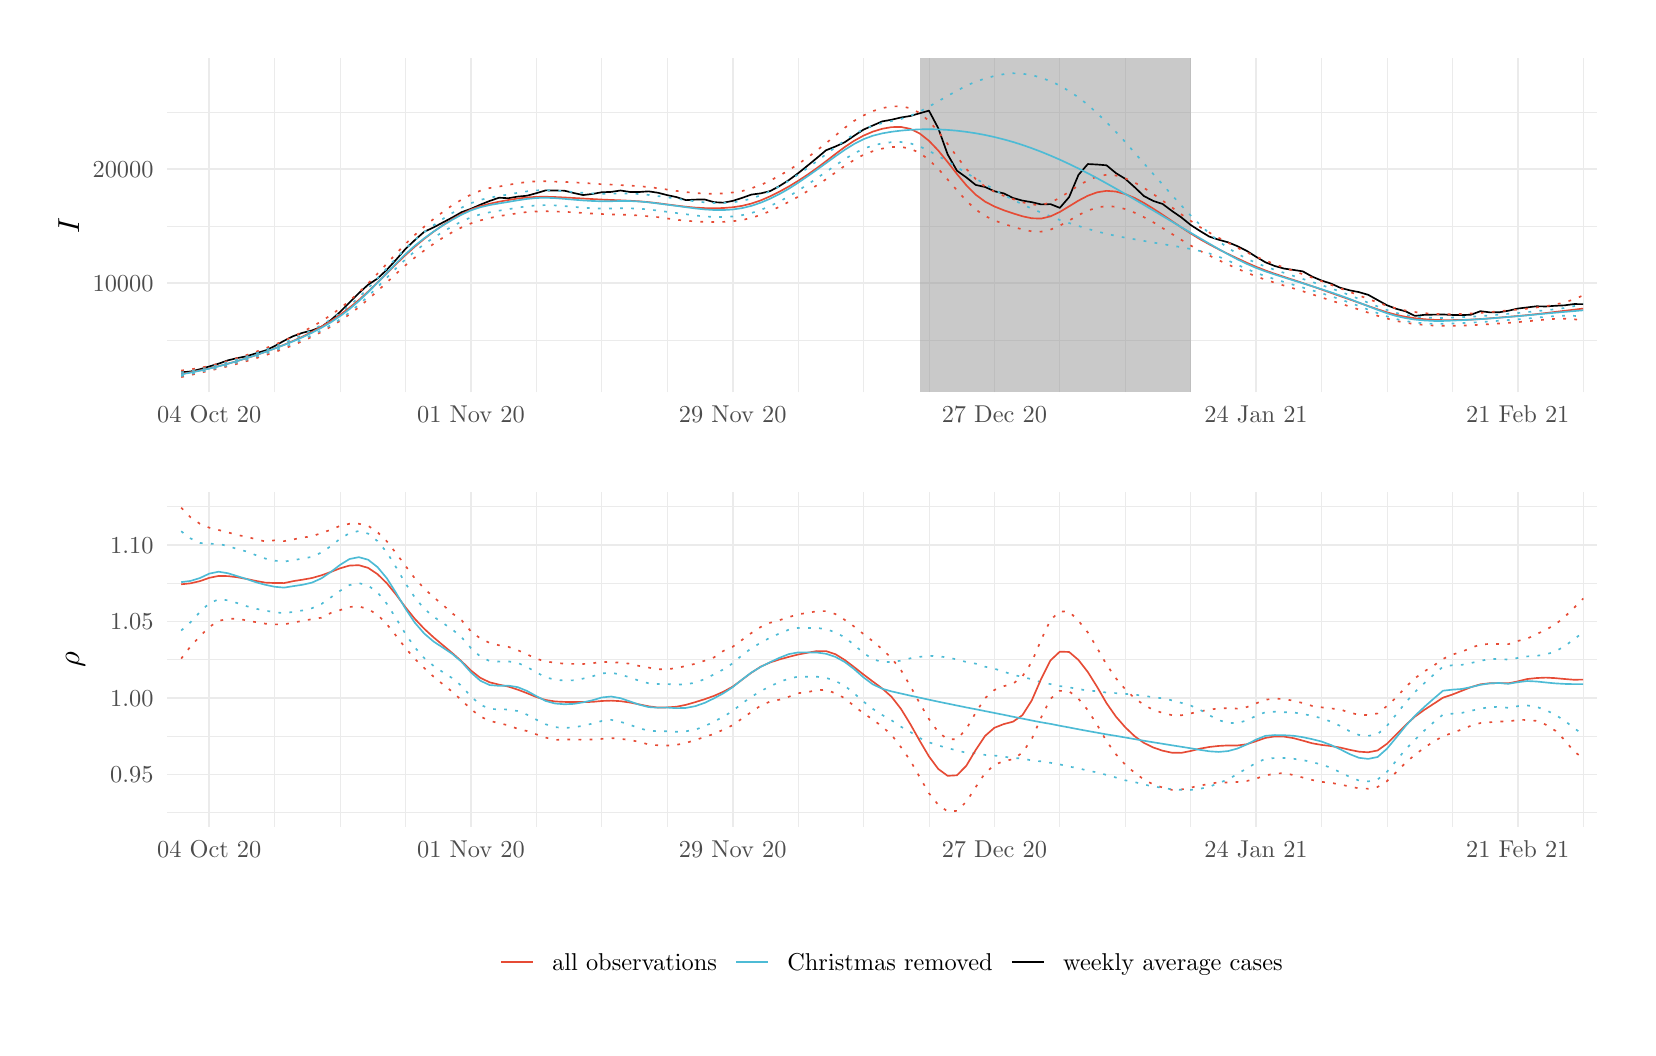
\begin{tikzpicture}[x=1pt,y=1pt]
\definecolor{fillColor}{RGB}{255,255,255}
\path[use as bounding box,fill=fillColor,fill opacity=0.00] (0,0) rectangle (578.16,361.35);
\begin{scope}
\path[clip] ( 50.41,229.59) rectangle (567.16,350.35);
\definecolor{drawColor}{gray}{0.92}

\path[draw=drawColor,line width= 0.3pt,line join=round] ( 50.41,248.41) --
	(567.16,248.41);

\path[draw=drawColor,line width= 0.3pt,line join=round] ( 50.41,289.65) --
	(567.16,289.65);

\path[draw=drawColor,line width= 0.3pt,line join=round] ( 50.41,330.89) --
	(567.16,330.89);

\path[draw=drawColor,line width= 0.3pt,line join=round] ( 89.25,229.59) --
	( 89.25,350.35);

\path[draw=drawColor,line width= 0.3pt,line join=round] (112.89,229.59) --
	(112.89,350.35);

\path[draw=drawColor,line width= 0.3pt,line join=round] (136.53,229.59) --
	(136.53,350.35);

\path[draw=drawColor,line width= 0.3pt,line join=round] (183.82,229.59) --
	(183.82,350.35);

\path[draw=drawColor,line width= 0.3pt,line join=round] (207.46,229.59) --
	(207.46,350.35);

\path[draw=drawColor,line width= 0.3pt,line join=round] (231.10,229.59) --
	(231.10,350.35);

\path[draw=drawColor,line width= 0.3pt,line join=round] (278.39,229.59) --
	(278.39,350.35);

\path[draw=drawColor,line width= 0.3pt,line join=round] (302.03,229.59) --
	(302.03,350.35);

\path[draw=drawColor,line width= 0.3pt,line join=round] (325.67,229.59) --
	(325.67,350.35);

\path[draw=drawColor,line width= 0.3pt,line join=round] (372.96,229.59) --
	(372.96,350.35);

\path[draw=drawColor,line width= 0.3pt,line join=round] (396.60,229.59) --
	(396.60,350.35);

\path[draw=drawColor,line width= 0.3pt,line join=round] (420.24,229.59) --
	(420.24,350.35);

\path[draw=drawColor,line width= 0.3pt,line join=round] (467.53,229.59) --
	(467.53,350.35);

\path[draw=drawColor,line width= 0.3pt,line join=round] (491.17,229.59) --
	(491.17,350.35);

\path[draw=drawColor,line width= 0.3pt,line join=round] (514.81,229.59) --
	(514.81,350.35);

\path[draw=drawColor,line width= 0.3pt,line join=round] (562.09,229.59) --
	(562.09,350.35);

\path[draw=drawColor,line width= 0.6pt,line join=round] ( 50.41,269.03) --
	(567.16,269.03);

\path[draw=drawColor,line width= 0.6pt,line join=round] ( 50.41,310.27) --
	(567.16,310.27);

\path[draw=drawColor,line width= 0.6pt,line join=round] ( 65.61,229.59) --
	( 65.61,350.35);

\path[draw=drawColor,line width= 0.6pt,line join=round] (160.18,229.59) --
	(160.18,350.35);

\path[draw=drawColor,line width= 0.6pt,line join=round] (254.75,229.59) --
	(254.75,350.35);

\path[draw=drawColor,line width= 0.6pt,line join=round] (349.31,229.59) --
	(349.31,350.35);

\path[draw=drawColor,line width= 0.6pt,line join=round] (443.88,229.59) --
	(443.88,350.35);

\path[draw=drawColor,line width= 0.6pt,line join=round] (538.45,229.59) --
	(538.45,350.35);
\definecolor{fillColor}{RGB}{190,190,190}

\path[fill=fillColor,fill opacity=0.01] (322.29,229.59) rectangle (420.24,350.35);

\path[fill=fillColor,fill opacity=0.01] (322.29,229.59) rectangle (420.24,350.35);

\path[fill=fillColor,fill opacity=0.01] (322.29,229.59) rectangle (420.24,350.35);

\path[fill=fillColor,fill opacity=0.01] (322.29,229.59) rectangle (420.24,350.35);

\path[fill=fillColor,fill opacity=0.01] (322.29,229.59) rectangle (420.24,350.35);

\path[fill=fillColor,fill opacity=0.01] (322.29,229.59) rectangle (420.24,350.35);

\path[fill=fillColor,fill opacity=0.01] (322.29,229.59) rectangle (420.24,350.35);

\path[fill=fillColor,fill opacity=0.01] (322.29,229.59) rectangle (420.24,350.35);

\path[fill=fillColor,fill opacity=0.01] (322.29,229.59) rectangle (420.24,350.35);

\path[fill=fillColor,fill opacity=0.01] (322.29,229.59) rectangle (420.24,350.35);

\path[fill=fillColor,fill opacity=0.01] (322.29,229.59) rectangle (420.24,350.35);

\path[fill=fillColor,fill opacity=0.01] (322.29,229.59) rectangle (420.24,350.35);

\path[fill=fillColor,fill opacity=0.01] (322.29,229.59) rectangle (420.24,350.35);

\path[fill=fillColor,fill opacity=0.01] (322.29,229.59) rectangle (420.24,350.35);

\path[fill=fillColor,fill opacity=0.01] (322.29,229.59) rectangle (420.24,350.35);

\path[fill=fillColor,fill opacity=0.01] (322.29,229.59) rectangle (420.24,350.35);

\path[fill=fillColor,fill opacity=0.01] (322.29,229.59) rectangle (420.24,350.35);

\path[fill=fillColor,fill opacity=0.01] (322.29,229.59) rectangle (420.24,350.35);

\path[fill=fillColor,fill opacity=0.01] (322.29,229.59) rectangle (420.24,350.35);

\path[fill=fillColor,fill opacity=0.01] (322.29,229.59) rectangle (420.24,350.35);

\path[fill=fillColor,fill opacity=0.01] (322.29,229.59) rectangle (420.24,350.35);

\path[fill=fillColor,fill opacity=0.01] (322.29,229.59) rectangle (420.24,350.35);

\path[fill=fillColor,fill opacity=0.01] (322.29,229.59) rectangle (420.24,350.35);

\path[fill=fillColor,fill opacity=0.01] (322.29,229.59) rectangle (420.24,350.35);

\path[fill=fillColor,fill opacity=0.01] (322.29,229.59) rectangle (420.24,350.35);

\path[fill=fillColor,fill opacity=0.01] (322.29,229.59) rectangle (420.24,350.35);

\path[fill=fillColor,fill opacity=0.01] (322.29,229.59) rectangle (420.24,350.35);

\path[fill=fillColor,fill opacity=0.01] (322.29,229.59) rectangle (420.24,350.35);

\path[fill=fillColor,fill opacity=0.01] (322.29,229.59) rectangle (420.24,350.35);

\path[fill=fillColor,fill opacity=0.01] (322.29,229.59) rectangle (420.24,350.35);

\path[fill=fillColor,fill opacity=0.01] (322.29,229.59) rectangle (420.24,350.35);

\path[fill=fillColor,fill opacity=0.01] (322.29,229.59) rectangle (420.24,350.35);

\path[fill=fillColor,fill opacity=0.01] (322.29,229.59) rectangle (420.24,350.35);

\path[fill=fillColor,fill opacity=0.01] (322.29,229.59) rectangle (420.24,350.35);

\path[fill=fillColor,fill opacity=0.01] (322.29,229.59) rectangle (420.24,350.35);

\path[fill=fillColor,fill opacity=0.01] (322.29,229.59) rectangle (420.24,350.35);

\path[fill=fillColor,fill opacity=0.01] (322.29,229.59) rectangle (420.24,350.35);

\path[fill=fillColor,fill opacity=0.01] (322.29,229.59) rectangle (420.24,350.35);

\path[fill=fillColor,fill opacity=0.01] (322.29,229.59) rectangle (420.24,350.35);

\path[fill=fillColor,fill opacity=0.01] (322.29,229.59) rectangle (420.24,350.35);

\path[fill=fillColor,fill opacity=0.01] (322.29,229.59) rectangle (420.24,350.35);

\path[fill=fillColor,fill opacity=0.01] (322.29,229.59) rectangle (420.24,350.35);

\path[fill=fillColor,fill opacity=0.01] (322.29,229.59) rectangle (420.24,350.35);

\path[fill=fillColor,fill opacity=0.01] (322.29,229.59) rectangle (420.24,350.35);

\path[fill=fillColor,fill opacity=0.01] (322.29,229.59) rectangle (420.24,350.35);

\path[fill=fillColor,fill opacity=0.01] (322.29,229.59) rectangle (420.24,350.35);

\path[fill=fillColor,fill opacity=0.01] (322.29,229.59) rectangle (420.24,350.35);

\path[fill=fillColor,fill opacity=0.01] (322.29,229.59) rectangle (420.24,350.35);

\path[fill=fillColor,fill opacity=0.01] (322.29,229.59) rectangle (420.24,350.35);

\path[fill=fillColor,fill opacity=0.01] (322.29,229.59) rectangle (420.24,350.35);

\path[fill=fillColor,fill opacity=0.01] (322.29,229.59) rectangle (420.24,350.35);

\path[fill=fillColor,fill opacity=0.01] (322.29,229.59) rectangle (420.24,350.35);

\path[fill=fillColor,fill opacity=0.01] (322.29,229.59) rectangle (420.24,350.35);

\path[fill=fillColor,fill opacity=0.01] (322.29,229.59) rectangle (420.24,350.35);

\path[fill=fillColor,fill opacity=0.01] (322.29,229.59) rectangle (420.24,350.35);

\path[fill=fillColor,fill opacity=0.01] (322.29,229.59) rectangle (420.24,350.35);

\path[fill=fillColor,fill opacity=0.01] (322.29,229.59) rectangle (420.24,350.35);

\path[fill=fillColor,fill opacity=0.01] (322.29,229.59) rectangle (420.24,350.35);

\path[fill=fillColor,fill opacity=0.01] (322.29,229.59) rectangle (420.24,350.35);

\path[fill=fillColor,fill opacity=0.01] (322.29,229.59) rectangle (420.24,350.35);

\path[fill=fillColor,fill opacity=0.01] (322.29,229.59) rectangle (420.24,350.35);

\path[fill=fillColor,fill opacity=0.01] (322.29,229.59) rectangle (420.24,350.35);

\path[fill=fillColor,fill opacity=0.01] (322.29,229.59) rectangle (420.24,350.35);

\path[fill=fillColor,fill opacity=0.01] (322.29,229.59) rectangle (420.24,350.35);

\path[fill=fillColor,fill opacity=0.01] (322.29,229.59) rectangle (420.24,350.35);

\path[fill=fillColor,fill opacity=0.01] (322.29,229.59) rectangle (420.24,350.35);

\path[fill=fillColor,fill opacity=0.01] (322.29,229.59) rectangle (420.24,350.35);

\path[fill=fillColor,fill opacity=0.01] (322.29,229.59) rectangle (420.24,350.35);

\path[fill=fillColor,fill opacity=0.01] (322.29,229.59) rectangle (420.24,350.35);

\path[fill=fillColor,fill opacity=0.01] (322.29,229.59) rectangle (420.24,350.35);

\path[fill=fillColor,fill opacity=0.01] (322.29,229.59) rectangle (420.24,350.35);

\path[fill=fillColor,fill opacity=0.01] (322.29,229.59) rectangle (420.24,350.35);

\path[fill=fillColor,fill opacity=0.01] (322.29,229.59) rectangle (420.24,350.35);

\path[fill=fillColor,fill opacity=0.01] (322.29,229.59) rectangle (420.24,350.35);

\path[fill=fillColor,fill opacity=0.01] (322.29,229.59) rectangle (420.24,350.35);

\path[fill=fillColor,fill opacity=0.01] (322.29,229.59) rectangle (420.24,350.35);

\path[fill=fillColor,fill opacity=0.01] (322.29,229.59) rectangle (420.24,350.35);

\path[fill=fillColor,fill opacity=0.01] (322.29,229.59) rectangle (420.24,350.35);

\path[fill=fillColor,fill opacity=0.01] (322.29,229.59) rectangle (420.24,350.35);

\path[fill=fillColor,fill opacity=0.01] (322.29,229.59) rectangle (420.24,350.35);

\path[fill=fillColor,fill opacity=0.01] (322.29,229.59) rectangle (420.24,350.35);

\path[fill=fillColor,fill opacity=0.01] (322.29,229.59) rectangle (420.24,350.35);

\path[fill=fillColor,fill opacity=0.01] (322.29,229.59) rectangle (420.24,350.35);

\path[fill=fillColor,fill opacity=0.01] (322.29,229.59) rectangle (420.24,350.35);

\path[fill=fillColor,fill opacity=0.01] (322.29,229.59) rectangle (420.24,350.35);

\path[fill=fillColor,fill opacity=0.01] (322.29,229.59) rectangle (420.24,350.35);

\path[fill=fillColor,fill opacity=0.01] (322.29,229.59) rectangle (420.24,350.35);

\path[fill=fillColor,fill opacity=0.01] (322.29,229.59) rectangle (420.24,350.35);

\path[fill=fillColor,fill opacity=0.01] (322.29,229.59) rectangle (420.24,350.35);

\path[fill=fillColor,fill opacity=0.01] (322.29,229.59) rectangle (420.24,350.35);

\path[fill=fillColor,fill opacity=0.01] (322.29,229.59) rectangle (420.24,350.35);

\path[fill=fillColor,fill opacity=0.01] (322.29,229.59) rectangle (420.24,350.35);

\path[fill=fillColor,fill opacity=0.01] (322.29,229.59) rectangle (420.24,350.35);

\path[fill=fillColor,fill opacity=0.01] (322.29,229.59) rectangle (420.24,350.35);

\path[fill=fillColor,fill opacity=0.01] (322.29,229.59) rectangle (420.24,350.35);

\path[fill=fillColor,fill opacity=0.01] (322.29,229.59) rectangle (420.24,350.35);

\path[fill=fillColor,fill opacity=0.01] (322.29,229.59) rectangle (420.24,350.35);

\path[fill=fillColor,fill opacity=0.01] (322.29,229.59) rectangle (420.24,350.35);

\path[fill=fillColor,fill opacity=0.01] (322.29,229.59) rectangle (420.24,350.35);

\path[fill=fillColor,fill opacity=0.01] (322.29,229.59) rectangle (420.24,350.35);

\path[fill=fillColor,fill opacity=0.01] (322.29,229.59) rectangle (420.24,350.35);

\path[fill=fillColor,fill opacity=0.01] (322.29,229.59) rectangle (420.24,350.35);

\path[fill=fillColor,fill opacity=0.01] (322.29,229.59) rectangle (420.24,350.35);

\path[fill=fillColor,fill opacity=0.01] (322.29,229.59) rectangle (420.24,350.35);

\path[fill=fillColor,fill opacity=0.01] (322.29,229.59) rectangle (420.24,350.35);

\path[fill=fillColor,fill opacity=0.01] (322.29,229.59) rectangle (420.24,350.35);

\path[fill=fillColor,fill opacity=0.01] (322.29,229.59) rectangle (420.24,350.35);

\path[fill=fillColor,fill opacity=0.01] (322.29,229.59) rectangle (420.24,350.35);

\path[fill=fillColor,fill opacity=0.01] (322.29,229.59) rectangle (420.24,350.35);

\path[fill=fillColor,fill opacity=0.01] (322.29,229.59) rectangle (420.24,350.35);

\path[fill=fillColor,fill opacity=0.01] (322.29,229.59) rectangle (420.24,350.35);

\path[fill=fillColor,fill opacity=0.01] (322.29,229.59) rectangle (420.24,350.35);

\path[fill=fillColor,fill opacity=0.01] (322.29,229.59) rectangle (420.24,350.35);

\path[fill=fillColor,fill opacity=0.01] (322.29,229.59) rectangle (420.24,350.35);

\path[fill=fillColor,fill opacity=0.01] (322.29,229.59) rectangle (420.24,350.35);

\path[fill=fillColor,fill opacity=0.01] (322.29,229.59) rectangle (420.24,350.35);

\path[fill=fillColor,fill opacity=0.01] (322.29,229.59) rectangle (420.24,350.35);

\path[fill=fillColor,fill opacity=0.01] (322.29,229.59) rectangle (420.24,350.35);

\path[fill=fillColor,fill opacity=0.01] (322.29,229.59) rectangle (420.24,350.35);

\path[fill=fillColor,fill opacity=0.01] (322.29,229.59) rectangle (420.24,350.35);

\path[fill=fillColor,fill opacity=0.01] (322.29,229.59) rectangle (420.24,350.35);

\path[fill=fillColor,fill opacity=0.01] (322.29,229.59) rectangle (420.24,350.35);

\path[fill=fillColor,fill opacity=0.01] (322.29,229.59) rectangle (420.24,350.35);

\path[fill=fillColor,fill opacity=0.01] (322.29,229.59) rectangle (420.24,350.35);

\path[fill=fillColor,fill opacity=0.01] (322.29,229.59) rectangle (420.24,350.35);

\path[fill=fillColor,fill opacity=0.01] (322.29,229.59) rectangle (420.24,350.35);

\path[fill=fillColor,fill opacity=0.01] (322.29,229.59) rectangle (420.24,350.35);

\path[fill=fillColor,fill opacity=0.01] (322.29,229.59) rectangle (420.24,350.35);

\path[fill=fillColor,fill opacity=0.01] (322.29,229.59) rectangle (420.24,350.35);

\path[fill=fillColor,fill opacity=0.01] (322.29,229.59) rectangle (420.24,350.35);

\path[fill=fillColor,fill opacity=0.01] (322.29,229.59) rectangle (420.24,350.35);

\path[fill=fillColor,fill opacity=0.01] (322.29,229.59) rectangle (420.24,350.35);

\path[fill=fillColor,fill opacity=0.01] (322.29,229.59) rectangle (420.24,350.35);

\path[fill=fillColor,fill opacity=0.01] (322.29,229.59) rectangle (420.24,350.35);

\path[fill=fillColor,fill opacity=0.01] (322.29,229.59) rectangle (420.24,350.35);

\path[fill=fillColor,fill opacity=0.01] (322.29,229.59) rectangle (420.24,350.35);

\path[fill=fillColor,fill opacity=0.01] (322.29,229.59) rectangle (420.24,350.35);

\path[fill=fillColor,fill opacity=0.01] (322.29,229.59) rectangle (420.24,350.35);

\path[fill=fillColor,fill opacity=0.01] (322.29,229.59) rectangle (420.24,350.35);

\path[fill=fillColor,fill opacity=0.01] (322.29,229.59) rectangle (420.24,350.35);

\path[fill=fillColor,fill opacity=0.01] (322.29,229.59) rectangle (420.24,350.35);

\path[fill=fillColor,fill opacity=0.01] (322.29,229.59) rectangle (420.24,350.35);

\path[fill=fillColor,fill opacity=0.01] (322.29,229.59) rectangle (420.24,350.35);

\path[fill=fillColor,fill opacity=0.01] (322.29,229.59) rectangle (420.24,350.35);

\path[fill=fillColor,fill opacity=0.01] (322.29,229.59) rectangle (420.24,350.35);

\path[fill=fillColor,fill opacity=0.01] (322.29,229.59) rectangle (420.24,350.35);

\path[fill=fillColor,fill opacity=0.01] (322.29,229.59) rectangle (420.24,350.35);

\path[fill=fillColor,fill opacity=0.01] (322.29,229.59) rectangle (420.24,350.35);

\path[fill=fillColor,fill opacity=0.01] (322.29,229.59) rectangle (420.24,350.35);

\path[fill=fillColor,fill opacity=0.01] (322.29,229.59) rectangle (420.24,350.35);

\path[fill=fillColor,fill opacity=0.01] (322.29,229.59) rectangle (420.24,350.35);

\path[fill=fillColor,fill opacity=0.01] (322.29,229.59) rectangle (420.24,350.35);

\path[fill=fillColor,fill opacity=0.01] (322.29,229.59) rectangle (420.24,350.35);

\path[fill=fillColor,fill opacity=0.01] (322.29,229.59) rectangle (420.24,350.35);

\path[fill=fillColor,fill opacity=0.01] (322.29,229.59) rectangle (420.24,350.35);

\path[fill=fillColor,fill opacity=0.01] (322.29,229.59) rectangle (420.24,350.35);

\path[fill=fillColor,fill opacity=0.01] (322.29,229.59) rectangle (420.24,350.35);

\path[fill=fillColor,fill opacity=0.01] (322.29,229.59) rectangle (420.24,350.35);

\path[fill=fillColor,fill opacity=0.01] (322.29,229.59) rectangle (420.24,350.35);

\path[fill=fillColor,fill opacity=0.01] (322.29,229.59) rectangle (420.24,350.35);

\path[fill=fillColor,fill opacity=0.01] (322.29,229.59) rectangle (420.24,350.35);

\path[fill=fillColor,fill opacity=0.01] (322.29,229.59) rectangle (420.24,350.35);

\path[fill=fillColor,fill opacity=0.01] (322.29,229.59) rectangle (420.24,350.35);

\path[fill=fillColor,fill opacity=0.01] (322.29,229.59) rectangle (420.24,350.35);

\path[fill=fillColor,fill opacity=0.01] (322.29,229.59) rectangle (420.24,350.35);

\path[fill=fillColor,fill opacity=0.01] (322.29,229.59) rectangle (420.24,350.35);

\path[fill=fillColor,fill opacity=0.01] (322.29,229.59) rectangle (420.24,350.35);

\path[fill=fillColor,fill opacity=0.01] (322.29,229.59) rectangle (420.24,350.35);

\path[fill=fillColor,fill opacity=0.01] (322.29,229.59) rectangle (420.24,350.35);

\path[fill=fillColor,fill opacity=0.01] (322.29,229.59) rectangle (420.24,350.35);

\path[fill=fillColor,fill opacity=0.01] (322.29,229.59) rectangle (420.24,350.35);

\path[fill=fillColor,fill opacity=0.01] (322.29,229.59) rectangle (420.24,350.35);

\path[fill=fillColor,fill opacity=0.01] (322.29,229.59) rectangle (420.24,350.35);

\path[fill=fillColor,fill opacity=0.01] (322.29,229.59) rectangle (420.24,350.35);

\path[fill=fillColor,fill opacity=0.01] (322.29,229.59) rectangle (420.24,350.35);

\path[fill=fillColor,fill opacity=0.01] (322.29,229.59) rectangle (420.24,350.35);

\path[fill=fillColor,fill opacity=0.01] (322.29,229.59) rectangle (420.24,350.35);

\path[fill=fillColor,fill opacity=0.01] (322.29,229.59) rectangle (420.24,350.35);

\path[fill=fillColor,fill opacity=0.01] (322.29,229.59) rectangle (420.24,350.35);

\path[fill=fillColor,fill opacity=0.01] (322.29,229.59) rectangle (420.24,350.35);

\path[fill=fillColor,fill opacity=0.01] (322.29,229.59) rectangle (420.24,350.35);

\path[fill=fillColor,fill opacity=0.01] (322.29,229.59) rectangle (420.24,350.35);

\path[fill=fillColor,fill opacity=0.01] (322.29,229.59) rectangle (420.24,350.35);

\path[fill=fillColor,fill opacity=0.01] (322.29,229.59) rectangle (420.24,350.35);

\path[fill=fillColor,fill opacity=0.01] (322.29,229.59) rectangle (420.24,350.35);

\path[fill=fillColor,fill opacity=0.01] (322.29,229.59) rectangle (420.24,350.35);

\path[fill=fillColor,fill opacity=0.01] (322.29,229.59) rectangle (420.24,350.35);

\path[fill=fillColor,fill opacity=0.01] (322.29,229.59) rectangle (420.24,350.35);

\path[fill=fillColor,fill opacity=0.01] (322.29,229.59) rectangle (420.24,350.35);

\path[fill=fillColor,fill opacity=0.01] (322.29,229.59) rectangle (420.24,350.35);

\path[fill=fillColor,fill opacity=0.01] (322.29,229.59) rectangle (420.24,350.35);

\path[fill=fillColor,fill opacity=0.01] (322.29,229.59) rectangle (420.24,350.35);

\path[fill=fillColor,fill opacity=0.01] (322.29,229.59) rectangle (420.24,350.35);

\path[fill=fillColor,fill opacity=0.01] (322.29,229.59) rectangle (420.24,350.35);

\path[fill=fillColor,fill opacity=0.01] (322.29,229.59) rectangle (420.24,350.35);

\path[fill=fillColor,fill opacity=0.01] (322.29,229.59) rectangle (420.24,350.35);

\path[fill=fillColor,fill opacity=0.01] (322.29,229.59) rectangle (420.24,350.35);

\path[fill=fillColor,fill opacity=0.01] (322.29,229.59) rectangle (420.24,350.35);

\path[fill=fillColor,fill opacity=0.01] (322.29,229.59) rectangle (420.24,350.35);

\path[fill=fillColor,fill opacity=0.01] (322.29,229.59) rectangle (420.24,350.35);

\path[fill=fillColor,fill opacity=0.01] (322.29,229.59) rectangle (420.24,350.35);

\path[fill=fillColor,fill opacity=0.01] (322.29,229.59) rectangle (420.24,350.35);

\path[fill=fillColor,fill opacity=0.01] (322.29,229.59) rectangle (420.24,350.35);

\path[fill=fillColor,fill opacity=0.01] (322.29,229.59) rectangle (420.24,350.35);

\path[fill=fillColor,fill opacity=0.01] (322.29,229.59) rectangle (420.24,350.35);

\path[fill=fillColor,fill opacity=0.01] (322.29,229.59) rectangle (420.24,350.35);

\path[fill=fillColor,fill opacity=0.01] (322.29,229.59) rectangle (420.24,350.35);

\path[fill=fillColor,fill opacity=0.01] (322.29,229.59) rectangle (420.24,350.35);

\path[fill=fillColor,fill opacity=0.01] (322.29,229.59) rectangle (420.24,350.35);

\path[fill=fillColor,fill opacity=0.01] (322.29,229.59) rectangle (420.24,350.35);

\path[fill=fillColor,fill opacity=0.01] (322.29,229.59) rectangle (420.24,350.35);

\path[fill=fillColor,fill opacity=0.01] (322.29,229.59) rectangle (420.24,350.35);

\path[fill=fillColor,fill opacity=0.01] (322.29,229.59) rectangle (420.24,350.35);

\path[fill=fillColor,fill opacity=0.01] (322.29,229.59) rectangle (420.24,350.35);

\path[fill=fillColor,fill opacity=0.01] (322.29,229.59) rectangle (420.24,350.35);

\path[fill=fillColor,fill opacity=0.01] (322.29,229.59) rectangle (420.24,350.35);

\path[fill=fillColor,fill opacity=0.01] (322.29,229.59) rectangle (420.24,350.35);

\path[fill=fillColor,fill opacity=0.01] (322.29,229.59) rectangle (420.24,350.35);

\path[fill=fillColor,fill opacity=0.01] (322.29,229.59) rectangle (420.24,350.35);

\path[fill=fillColor,fill opacity=0.01] (322.29,229.59) rectangle (420.24,350.35);

\path[fill=fillColor,fill opacity=0.01] (322.29,229.59) rectangle (420.24,350.35);

\path[fill=fillColor,fill opacity=0.01] (322.29,229.59) rectangle (420.24,350.35);

\path[fill=fillColor,fill opacity=0.01] (322.29,229.59) rectangle (420.24,350.35);

\path[fill=fillColor,fill opacity=0.01] (322.29,229.59) rectangle (420.24,350.35);

\path[fill=fillColor,fill opacity=0.01] (322.29,229.59) rectangle (420.24,350.35);

\path[fill=fillColor,fill opacity=0.01] (322.29,229.59) rectangle (420.24,350.35);

\path[fill=fillColor,fill opacity=0.01] (322.29,229.59) rectangle (420.24,350.35);

\path[fill=fillColor,fill opacity=0.01] (322.29,229.59) rectangle (420.24,350.35);

\path[fill=fillColor,fill opacity=0.01] (322.29,229.59) rectangle (420.24,350.35);

\path[fill=fillColor,fill opacity=0.01] (322.29,229.59) rectangle (420.24,350.35);

\path[fill=fillColor,fill opacity=0.01] (322.29,229.59) rectangle (420.24,350.35);

\path[fill=fillColor,fill opacity=0.01] (322.29,229.59) rectangle (420.24,350.35);

\path[fill=fillColor,fill opacity=0.01] (322.29,229.59) rectangle (420.24,350.35);

\path[fill=fillColor,fill opacity=0.01] (322.29,229.59) rectangle (420.24,350.35);

\path[fill=fillColor,fill opacity=0.01] (322.29,229.59) rectangle (420.24,350.35);

\path[fill=fillColor,fill opacity=0.01] (322.29,229.59) rectangle (420.24,350.35);

\path[fill=fillColor,fill opacity=0.01] (322.29,229.59) rectangle (420.24,350.35);

\path[fill=fillColor,fill opacity=0.01] (322.29,229.59) rectangle (420.24,350.35);

\path[fill=fillColor,fill opacity=0.01] (322.29,229.59) rectangle (420.24,350.35);

\path[fill=fillColor,fill opacity=0.01] (322.29,229.59) rectangle (420.24,350.35);

\path[fill=fillColor,fill opacity=0.01] (322.29,229.59) rectangle (420.24,350.35);

\path[fill=fillColor,fill opacity=0.01] (322.29,229.59) rectangle (420.24,350.35);

\path[fill=fillColor,fill opacity=0.01] (322.29,229.59) rectangle (420.24,350.35);

\path[fill=fillColor,fill opacity=0.01] (322.29,229.59) rectangle (420.24,350.35);

\path[fill=fillColor,fill opacity=0.01] (322.29,229.59) rectangle (420.24,350.35);

\path[fill=fillColor,fill opacity=0.01] (322.29,229.59) rectangle (420.24,350.35);

\path[fill=fillColor,fill opacity=0.01] (322.29,229.59) rectangle (420.24,350.35);

\path[fill=fillColor,fill opacity=0.01] (322.29,229.59) rectangle (420.24,350.35);

\path[fill=fillColor,fill opacity=0.01] (322.29,229.59) rectangle (420.24,350.35);

\path[fill=fillColor,fill opacity=0.01] (322.29,229.59) rectangle (420.24,350.35);

\path[fill=fillColor,fill opacity=0.01] (322.29,229.59) rectangle (420.24,350.35);

\path[fill=fillColor,fill opacity=0.01] (322.29,229.59) rectangle (420.24,350.35);

\path[fill=fillColor,fill opacity=0.01] (322.29,229.59) rectangle (420.24,350.35);

\path[fill=fillColor,fill opacity=0.01] (322.29,229.59) rectangle (420.24,350.35);

\path[fill=fillColor,fill opacity=0.01] (322.29,229.59) rectangle (420.24,350.35);

\path[fill=fillColor,fill opacity=0.01] (322.29,229.59) rectangle (420.24,350.35);

\path[fill=fillColor,fill opacity=0.01] (322.29,229.59) rectangle (420.24,350.35);

\path[fill=fillColor,fill opacity=0.01] (322.29,229.59) rectangle (420.24,350.35);

\path[fill=fillColor,fill opacity=0.01] (322.29,229.59) rectangle (420.24,350.35);

\path[fill=fillColor,fill opacity=0.01] (322.29,229.59) rectangle (420.24,350.35);

\path[fill=fillColor,fill opacity=0.01] (322.29,229.59) rectangle (420.24,350.35);

\path[fill=fillColor,fill opacity=0.01] (322.29,229.59) rectangle (420.24,350.35);

\path[fill=fillColor,fill opacity=0.01] (322.29,229.59) rectangle (420.24,350.35);

\path[fill=fillColor,fill opacity=0.01] (322.29,229.59) rectangle (420.24,350.35);

\path[fill=fillColor,fill opacity=0.01] (322.29,229.59) rectangle (420.24,350.35);

\path[fill=fillColor,fill opacity=0.01] (322.29,229.59) rectangle (420.24,350.35);

\path[fill=fillColor,fill opacity=0.01] (322.29,229.59) rectangle (420.24,350.35);

\path[fill=fillColor,fill opacity=0.01] (322.29,229.59) rectangle (420.24,350.35);

\path[fill=fillColor,fill opacity=0.01] (322.29,229.59) rectangle (420.24,350.35);

\path[fill=fillColor,fill opacity=0.01] (322.29,229.59) rectangle (420.24,350.35);

\path[fill=fillColor,fill opacity=0.01] (322.29,229.59) rectangle (420.24,350.35);

\path[fill=fillColor,fill opacity=0.01] (322.29,229.59) rectangle (420.24,350.35);

\path[fill=fillColor,fill opacity=0.01] (322.29,229.59) rectangle (420.24,350.35);

\path[fill=fillColor,fill opacity=0.01] (322.29,229.59) rectangle (420.24,350.35);

\path[fill=fillColor,fill opacity=0.01] (322.29,229.59) rectangle (420.24,350.35);

\path[fill=fillColor,fill opacity=0.01] (322.29,229.59) rectangle (420.24,350.35);

\path[fill=fillColor,fill opacity=0.01] (322.29,229.59) rectangle (420.24,350.35);

\path[fill=fillColor,fill opacity=0.01] (322.29,229.59) rectangle (420.24,350.35);

\path[fill=fillColor,fill opacity=0.01] (322.29,229.59) rectangle (420.24,350.35);

\path[fill=fillColor,fill opacity=0.01] (322.29,229.59) rectangle (420.24,350.35);

\path[fill=fillColor,fill opacity=0.01] (322.29,229.59) rectangle (420.24,350.35);

\path[fill=fillColor,fill opacity=0.01] (322.29,229.59) rectangle (420.24,350.35);

\path[fill=fillColor,fill opacity=0.01] (322.29,229.59) rectangle (420.24,350.35);

\path[fill=fillColor,fill opacity=0.01] (322.29,229.59) rectangle (420.24,350.35);

\path[fill=fillColor,fill opacity=0.01] (322.29,229.59) rectangle (420.24,350.35);

\path[fill=fillColor,fill opacity=0.01] (322.29,229.59) rectangle (420.24,350.35);

\path[fill=fillColor,fill opacity=0.01] (322.29,229.59) rectangle (420.24,350.35);

\path[fill=fillColor,fill opacity=0.01] (322.29,229.59) rectangle (420.24,350.35);

\path[fill=fillColor,fill opacity=0.01] (322.29,229.59) rectangle (420.24,350.35);

\path[fill=fillColor,fill opacity=0.01] (322.29,229.59) rectangle (420.24,350.35);

\path[fill=fillColor,fill opacity=0.01] (322.29,229.59) rectangle (420.24,350.35);

\path[fill=fillColor,fill opacity=0.01] (322.29,229.59) rectangle (420.24,350.35);

\path[fill=fillColor,fill opacity=0.01] (322.29,229.59) rectangle (420.24,350.35);

\path[fill=fillColor,fill opacity=0.01] (322.29,229.59) rectangle (420.24,350.35);

\path[fill=fillColor,fill opacity=0.01] (322.29,229.59) rectangle (420.24,350.35);

\path[fill=fillColor,fill opacity=0.01] (322.29,229.59) rectangle (420.24,350.35);

\path[fill=fillColor,fill opacity=0.01] (322.29,229.59) rectangle (420.24,350.35);

\path[fill=fillColor,fill opacity=0.01] (322.29,229.59) rectangle (420.24,350.35);

\path[fill=fillColor,fill opacity=0.01] (322.29,229.59) rectangle (420.24,350.35);

\path[fill=fillColor,fill opacity=0.01] (322.29,229.59) rectangle (420.24,350.35);

\path[fill=fillColor,fill opacity=0.01] (322.29,229.59) rectangle (420.24,350.35);

\path[fill=fillColor,fill opacity=0.01] (322.29,229.59) rectangle (420.24,350.35);
\definecolor{drawColor}{RGB}{0,0,0}

\path[draw=drawColor,line width= 0.6pt,line join=round] ( 55.48,236.80) --
	( 58.85,237.11) --
	( 62.23,237.92) --
	( 65.61,238.92) --
	( 68.99,239.93) --
	( 72.36,241.14) --
	( 75.74,241.95) --
	( 79.12,242.62) --
	( 82.49,243.67) --
	( 85.87,244.69) --
	( 89.25,246.29) --
	( 92.63,248.20) --
	( 96.00,249.89) --
	( 99.38,251.11) --
	(102.76,251.94) --
	(106.14,253.26) --
	(109.51,255.65) --
	(112.89,258.62) --
	(116.27,262.00) --
	(119.65,265.39) --
	(123.02,268.47) --
	(126.40,270.68) --
	(129.78,273.86) --
	(133.16,277.54) --
	(136.53,281.41) --
	(139.91,284.60) --
	(143.29,287.59) --
	(146.67,289.17) --
	(150.04,290.96) --
	(153.42,292.75) --
	(156.80,294.68) --
	(160.18,295.89) --
	(163.55,297.37) --
	(166.93,298.72) --
	(170.31,299.90) --
	(173.69,299.72) --
	(177.06,300.30) --
	(180.44,300.61) --
	(183.82,301.54) --
	(187.20,302.55) --
	(190.57,302.50) --
	(193.95,302.44) --
	(197.33,301.60) --
	(200.71,300.86) --
	(204.08,301.26) --
	(207.46,301.88) --
	(210.84,302.00) --
	(214.22,302.51) --
	(217.59,301.99) --
	(220.97,301.97) --
	(224.35,302.20) --
	(227.73,301.70) --
	(231.10,300.84) --
	(234.48,300.12) --
	(237.86,299.03) --
	(241.24,299.22) --
	(244.61,299.28) --
	(247.99,298.29) --
	(251.37,298.11) --
	(254.75,298.75) --
	(258.12,299.82) --
	(261.50,301.03) --
	(264.88,301.47) --
	(268.26,302.28) --
	(271.63,304.10) --
	(275.01,306.24) --
	(278.39,308.73) --
	(281.76,311.45) --
	(285.14,314.22) --
	(288.52,317.07) --
	(291.90,318.41) --
	(295.27,319.96) --
	(298.65,322.30) --
	(302.03,324.50) --
	(305.41,326.01) --
	(308.78,327.48) --
	(312.16,328.08) --
	(315.54,328.88) --
	(318.92,329.43) --
	(322.29,330.40) --
	(325.67,331.36) --
	(329.05,324.99) --
	(332.43,315.55) --
	(335.80,309.65) --
	(339.18,307.24) --
	(342.56,304.52) --
	(345.94,303.78) --
	(349.31,302.25) --
	(352.69,301.46) --
	(356.07,299.80) --
	(359.45,298.86) --
	(362.82,298.29) --
	(366.20,297.48) --
	(369.58,297.59) --
	(372.96,296.23) --
	(376.33,300.13) --
	(379.71,308.17) --
	(383.09,312.07) --
	(386.47,311.89) --
	(389.84,311.61) --
	(393.22,308.81) --
	(396.60,306.73) --
	(399.98,303.71) --
	(403.35,300.50) --
	(406.73,298.73) --
	(410.11,297.64) --
	(413.49,295.11) --
	(416.86,292.80) --
	(420.24,290.07) --
	(423.62,287.88) --
	(427.00,285.83) --
	(430.37,284.72) --
	(433.75,283.79) --
	(437.13,282.40) --
	(440.51,280.70) --
	(443.88,278.55) --
	(447.26,276.57) --
	(450.64,275.22) --
	(454.02,274.29) --
	(457.39,273.81) --
	(460.77,273.29) --
	(464.15,271.39) --
	(467.53,269.97) --
	(470.90,268.90) --
	(474.28,267.37) --
	(477.66,266.45) --
	(481.03,265.79) --
	(484.41,264.81) --
	(487.79,262.92) --
	(491.17,261.05) --
	(494.54,259.75) --
	(497.92,258.84) --
	(501.30,257.19) --
	(504.68,257.58) --
	(508.05,257.65) --
	(511.43,257.71) --
	(514.81,257.54) --
	(518.19,257.48) --
	(521.56,257.63) --
	(524.94,258.90) --
	(528.32,258.48) --
	(531.70,258.50) --
	(535.07,259.07) --
	(538.45,259.85) --
	(541.83,260.26) --
	(545.21,260.67) --
	(548.58,260.60) --
	(551.96,260.85) --
	(555.34,261.01) --
	(558.72,261.47) --
	(562.09,261.46);
\definecolor{drawColor}{RGB}{230,75,53}

\path[draw=drawColor,line width= 0.6pt,dash pattern=on 1pt off 3pt ,line join=round] ( 55.48,235.08) --
	( 58.85,235.83) --
	( 62.23,236.60) --
	( 65.61,237.38) --
	( 68.99,238.17) --
	( 72.36,239.01) --
	( 75.74,239.92) --
	( 79.12,240.87) --
	( 82.49,241.89) --
	( 85.87,242.97) --
	( 89.25,244.12) --
	( 92.63,245.33) --
	( 96.00,246.66) --
	( 99.38,248.11) --
	(102.76,249.68) --
	(106.14,251.40) --
	(109.51,253.30) --
	(112.89,255.41) --
	(116.27,257.74) --
	(119.65,260.33) --
	(123.02,263.19) --
	(126.40,266.18) --
	(129.78,269.29) --
	(133.16,272.45) --
	(136.53,275.50) --
	(139.91,278.28) --
	(143.29,280.82) --
	(146.67,283.22) --
	(150.04,285.44) --
	(153.42,287.44) --
	(156.80,289.17) --
	(160.18,290.62) --
	(163.55,291.69) --
	(166.93,292.55) --
	(170.31,293.26) --
	(173.69,293.76) --
	(177.06,294.29) --
	(180.44,294.73) --
	(183.82,294.94) --
	(187.20,295.00) --
	(190.57,294.92) --
	(193.95,294.79) --
	(197.33,294.62) --
	(200.71,294.37) --
	(204.08,294.17) --
	(207.46,294.00) --
	(210.84,293.86) --
	(214.22,293.78) --
	(217.59,293.69) --
	(220.97,293.46) --
	(224.35,293.19) --
	(227.73,292.87) --
	(231.10,292.40) --
	(234.48,291.93) --
	(237.86,291.59) --
	(241.24,291.33) --
	(244.61,291.17) --
	(247.99,291.11) --
	(251.37,291.17) --
	(254.75,291.40) --
	(258.12,291.83) --
	(261.50,292.61) --
	(264.88,293.69) --
	(268.26,295.05) --
	(271.63,296.65) --
	(275.01,298.39) --
	(278.39,300.25) --
	(281.76,302.26) --
	(285.14,304.35) --
	(288.52,306.59) --
	(291.90,309.03) --
	(295.27,311.45) --
	(298.65,313.55) --
	(302.03,315.44) --
	(305.41,316.71) --
	(308.78,317.64) --
	(312.16,318.21) --
	(315.54,318.29) --
	(318.92,317.60) --
	(322.29,316.12) --
	(325.67,313.60) --
	(329.05,310.34) --
	(332.43,306.48) --
	(335.80,302.57) --
	(339.18,298.81) --
	(342.56,295.65) --
	(345.94,293.32) --
	(349.31,291.70) --
	(352.69,290.47) --
	(356.07,289.37) --
	(359.45,288.44) --
	(362.82,287.74) --
	(366.20,287.63) --
	(369.58,288.36) --
	(372.96,289.81) --
	(376.33,291.65) --
	(379.71,293.62) --
	(383.09,295.23) --
	(386.47,296.38) --
	(389.84,296.87) --
	(393.22,296.62) --
	(396.60,295.81) --
	(399.98,294.50) --
	(403.35,292.88) --
	(406.73,291.04) --
	(410.11,288.92) --
	(413.49,286.81) --
	(416.86,284.68) --
	(420.24,282.63) --
	(423.62,280.72) --
	(427.00,278.98) --
	(430.37,277.32) --
	(433.75,275.75) --
	(437.13,274.24) --
	(440.51,272.82) --
	(443.88,271.50) --
	(447.26,270.27) --
	(450.64,269.18) --
	(454.02,268.15) --
	(457.39,267.14) --
	(460.77,266.10) --
	(464.15,265.00) --
	(467.53,263.87) --
	(470.90,262.78) --
	(474.28,261.68) --
	(477.66,260.60) --
	(481.03,259.49) --
	(484.41,258.37) --
	(487.79,257.24) --
	(491.17,256.24) --
	(494.54,255.37) --
	(497.92,254.71) --
	(501.30,254.24) --
	(504.68,253.94) --
	(508.05,253.71) --
	(511.43,253.62) --
	(514.81,253.63) --
	(518.19,253.67) --
	(521.56,253.80) --
	(524.94,254.01) --
	(528.32,254.23) --
	(531.70,254.46) --
	(535.07,254.69) --
	(538.45,254.94) --
	(541.83,255.23) --
	(545.21,255.57) --
	(548.58,255.89) --
	(551.96,256.13) --
	(555.34,256.17) --
	(558.72,256.00) --
	(562.09,255.51);
\definecolor{drawColor}{RGB}{77,187,213}

\path[draw=drawColor,line width= 0.6pt,dash pattern=on 1pt off 3pt ,line join=round] ( 55.48,235.47) --
	( 58.85,236.20) --
	( 62.23,236.92) --
	( 65.61,237.67) --
	( 68.99,238.49) --
	( 72.36,239.39) --
	( 75.74,240.35) --
	( 79.12,241.38) --
	( 82.49,242.45) --
	( 85.87,243.56) --
	( 89.25,244.72) --
	( 92.63,245.94) --
	( 96.00,247.26) --
	( 99.38,248.69) --
	(102.76,250.25) --
	(106.14,251.95) --
	(109.51,253.83) --
	(112.89,255.97) --
	(116.27,258.42) --
	(119.65,261.22) --
	(123.02,264.31) --
	(126.40,267.59) --
	(129.78,271.01) --
	(133.16,274.43) --
	(136.53,277.64) --
	(139.91,280.55) --
	(143.29,283.12) --
	(146.67,285.44) --
	(150.04,287.59) --
	(153.42,289.56) --
	(156.80,291.33) --
	(160.18,292.81) --
	(163.55,293.90) --
	(166.93,294.63) --
	(170.31,295.22) --
	(173.69,295.75) --
	(177.06,296.33) --
	(180.44,296.79) --
	(183.82,297.14) --
	(187.20,297.23) --
	(190.57,297.12) --
	(193.95,296.88) --
	(197.33,296.59) --
	(200.71,296.30) --
	(204.08,296.10) --
	(207.46,295.96) --
	(210.84,296.00) --
	(214.22,296.09) --
	(217.59,296.07) --
	(220.97,295.94) --
	(224.35,295.66) --
	(227.73,295.24) --
	(231.10,294.80) --
	(234.48,294.36) --
	(237.86,293.93) --
	(241.24,293.49) --
	(244.61,293.14) --
	(247.99,292.96) --
	(251.37,292.93) --
	(254.75,293.12) --
	(258.12,293.58) --
	(261.50,294.36) --
	(264.88,295.48) --
	(268.26,296.88) --
	(271.63,298.51) --
	(275.01,300.38) --
	(278.39,302.45) --
	(281.76,304.64) --
	(285.14,306.92) --
	(288.52,309.25) --
	(291.90,311.60) --
	(295.27,313.86) --
	(298.65,315.92) --
	(302.03,317.59) --
	(305.41,318.78) --
	(308.78,319.55) --
	(312.16,319.96) --
	(315.54,320.03) --
	(318.92,319.54) --
	(322.29,318.45) --
	(325.67,316.83) --
	(329.05,314.99) --
	(332.43,313.01) --
	(335.80,310.94) --
	(339.18,308.84) --
	(342.56,306.84) --
	(345.94,304.79) --
	(349.31,302.85) --
	(352.69,300.90) --
	(356.07,299.18) --
	(359.45,297.48) --
	(362.82,295.95) --
	(366.20,294.54) --
	(369.58,293.18) --
	(372.96,291.85) --
	(376.33,290.75) --
	(379.71,289.69) --
	(383.09,288.62) --
	(386.47,287.70) --
	(389.84,286.85) --
	(393.22,286.12) --
	(396.60,285.46) --
	(399.98,284.87) --
	(403.35,284.29) --
	(406.73,283.69) --
	(410.11,283.16) --
	(413.49,282.56) --
	(416.86,282.03) --
	(420.24,281.36) --
	(423.62,280.65) --
	(427.00,279.76) --
	(430.37,278.60) --
	(433.75,277.20) --
	(437.13,275.67) --
	(440.51,274.16) --
	(443.88,272.77) --
	(447.26,271.56) --
	(450.64,270.47) --
	(454.02,269.44) --
	(457.39,268.44) --
	(460.77,267.44) --
	(464.15,266.44) --
	(467.53,265.38) --
	(470.90,264.31) --
	(474.28,263.19) --
	(477.66,261.99) --
	(481.03,260.76) --
	(484.41,259.46) --
	(487.79,258.19) --
	(491.17,257.01) --
	(494.54,256.05) --
	(497.92,255.32) --
	(501.30,254.82) --
	(504.68,254.50) --
	(508.05,254.34) --
	(511.43,254.33) --
	(514.81,254.46) --
	(518.19,254.61) --
	(521.56,254.77) --
	(524.94,254.95) --
	(528.32,255.19) --
	(531.70,255.44) --
	(535.07,255.71) --
	(538.45,255.95) --
	(541.83,256.23) --
	(545.21,256.56) --
	(548.58,256.87) --
	(551.96,257.13) --
	(555.34,257.27) --
	(558.72,257.22) --
	(562.09,256.96);
\definecolor{drawColor}{RGB}{230,75,53}

\path[draw=drawColor,line width= 0.6pt,dash pattern=on 1pt off 3pt ,line join=round] ( 55.48,237.45) --
	( 58.85,237.86) --
	( 62.23,238.42) --
	( 65.61,239.11) --
	( 68.99,239.96) --
	( 72.36,240.91) --
	( 75.74,241.95) --
	( 79.12,243.06) --
	( 82.49,244.23) --
	( 85.87,245.48) --
	( 89.25,246.81) --
	( 92.63,248.24) --
	( 96.00,249.77) --
	( 99.38,251.45) --
	(102.76,253.27) --
	(106.14,255.26) --
	(109.51,257.47) --
	(112.89,259.91) --
	(116.27,262.63) --
	(119.65,265.66) --
	(123.02,268.95) --
	(126.40,272.45) --
	(129.78,276.06) --
	(133.16,279.70) --
	(136.53,283.22) --
	(139.91,286.48) --
	(143.29,289.42) --
	(146.67,292.20) --
	(150.04,294.76) --
	(153.42,297.16) --
	(156.80,299.20) --
	(160.18,301.05) --
	(163.55,302.42) --
	(166.93,303.39) --
	(170.31,303.92) --
	(173.69,304.56) --
	(177.06,305.10) --
	(180.44,305.60) --
	(183.82,305.83) --
	(187.20,305.88) --
	(190.57,305.71) --
	(193.95,305.61) --
	(197.33,305.44) --
	(200.71,305.24) --
	(204.08,305.01) --
	(207.46,304.77) --
	(210.84,304.64) --
	(214.22,304.46) --
	(217.59,304.27) --
	(220.97,304.07) --
	(224.35,303.75) --
	(227.73,303.33) --
	(231.10,302.85) --
	(234.48,302.35) --
	(237.86,301.93) --
	(241.24,301.59) --
	(244.61,301.38) --
	(247.99,301.32) --
	(251.37,301.46) --
	(254.75,301.79) --
	(258.12,302.29) --
	(261.50,303.31) --
	(264.88,304.48) --
	(268.26,306.04) --
	(271.63,307.88) --
	(275.01,309.80) --
	(278.39,312.05) --
	(281.76,314.36) --
	(285.14,316.94) --
	(288.52,319.63) --
	(291.90,322.39) --
	(295.27,325.17) --
	(298.65,327.68) --
	(302.03,329.63) --
	(305.41,331.21) --
	(308.78,332.28) --
	(312.16,332.90) --
	(315.54,332.94) --
	(318.92,332.24) --
	(322.29,330.54) --
	(325.67,327.63) --
	(329.05,323.76) --
	(332.43,319.34) --
	(335.80,314.75) --
	(339.18,310.32) --
	(342.56,306.65) --
	(345.94,303.93) --
	(349.31,302.06) --
	(352.69,300.60) --
	(356.07,299.41) --
	(359.45,298.27) --
	(362.82,297.42) --
	(366.20,297.31) --
	(369.58,298.15) --
	(372.96,299.90) --
	(376.33,302.06) --
	(379.71,304.32) --
	(383.09,306.16) --
	(386.47,307.56) --
	(389.84,308.20) --
	(393.22,307.93) --
	(396.60,306.91) --
	(399.98,305.39) --
	(403.35,303.48) --
	(406.73,301.22) --
	(410.11,298.85) --
	(413.49,296.39) --
	(416.86,293.90) --
	(420.24,291.55) --
	(423.62,289.28) --
	(427.00,287.30) --
	(430.37,285.42) --
	(433.75,283.63) --
	(437.13,281.86) --
	(440.51,280.15) --
	(443.88,278.59) --
	(447.26,277.20) --
	(450.64,275.87) --
	(454.02,274.64) --
	(457.39,273.47) --
	(460.77,272.25) --
	(464.15,271.01) --
	(467.53,269.75) --
	(470.90,268.45) --
	(474.28,267.17) --
	(477.66,265.91) --
	(481.03,264.59) --
	(484.41,263.32) --
	(487.79,262.06) --
	(491.17,260.87) --
	(494.54,259.88) --
	(497.92,259.12) --
	(501.30,258.59) --
	(504.68,258.19) --
	(508.05,257.93) --
	(511.43,257.82) --
	(514.81,257.82) --
	(518.19,257.88) --
	(521.56,258.06) --
	(524.94,258.29) --
	(528.32,258.56) --
	(531.70,258.88) --
	(535.07,259.18) --
	(538.45,259.49) --
	(541.83,259.82) --
	(545.21,260.26) --
	(548.58,260.70) --
	(551.96,261.30) --
	(555.34,262.08) --
	(558.72,263.17) --
	(562.09,264.62);
\definecolor{drawColor}{RGB}{77,187,213}

\path[draw=drawColor,line width= 0.6pt,dash pattern=on 1pt off 3pt ,line join=round] ( 55.48,236.72) --
	( 58.85,237.23) --
	( 62.23,237.86) --
	( 65.61,238.62) --
	( 68.99,239.48) --
	( 72.36,240.43) --
	( 75.74,241.45) --
	( 79.12,242.51) --
	( 82.49,243.64) --
	( 85.87,244.83) --
	( 89.25,246.09) --
	( 92.63,247.42) --
	( 96.00,248.83) --
	( 99.38,250.37) --
	(102.76,252.04) --
	(106.14,253.87) --
	(109.51,255.91) --
	(112.89,258.21) --
	(116.27,260.86) --
	(119.65,263.86) --
	(123.02,267.18) --
	(126.40,270.76) --
	(129.78,274.43) --
	(133.16,278.08) --
	(136.53,281.53) --
	(139.91,284.66) --
	(143.29,287.44) --
	(146.67,289.94) --
	(150.04,292.24) --
	(153.42,294.37) --
	(156.80,296.30) --
	(160.18,297.91) --
	(163.55,299.09) --
	(166.93,299.94) --
	(170.31,300.50) --
	(173.69,301.07) --
	(177.06,301.67) --
	(180.44,302.20) --
	(183.82,302.55) --
	(187.20,302.65) --
	(190.57,302.49) --
	(193.95,302.24) --
	(197.33,301.92) --
	(200.71,301.66) --
	(204.08,301.45) --
	(207.46,301.35) --
	(210.84,301.37) --
	(214.22,301.42) --
	(217.59,301.41) --
	(220.97,301.24) --
	(224.35,300.91) --
	(227.73,300.49) --
	(231.10,300.05) --
	(234.48,299.55) --
	(237.86,299.04) --
	(241.24,298.60) --
	(244.61,298.23) --
	(247.99,298.01) --
	(251.37,298.00) --
	(254.75,298.23) --
	(258.12,298.74) --
	(261.50,299.59) --
	(264.88,300.77) --
	(268.26,302.23) --
	(271.63,303.98) --
	(275.01,305.99) --
	(278.39,308.27) --
	(281.76,310.61) --
	(285.14,313.08) --
	(288.52,315.63) --
	(291.90,318.15) --
	(295.27,320.60) --
	(298.65,322.85) --
	(302.03,324.67) --
	(305.41,325.93) --
	(308.78,326.87) --
	(312.16,327.59) --
	(315.54,328.34) --
	(318.92,329.48) --
	(322.29,331.00) --
	(325.67,332.82) --
	(329.05,334.76) --
	(332.43,336.70) --
	(335.80,338.55) --
	(339.18,340.39) --
	(342.56,341.81) --
	(345.94,342.97) --
	(349.31,343.89) --
	(352.69,344.53) --
	(356.07,344.86) --
	(359.45,344.70) --
	(362.82,344.24) --
	(366.20,343.26) --
	(369.58,342.00) --
	(372.96,340.45) --
	(376.33,338.41) --
	(379.71,336.15) --
	(383.09,333.47) --
	(386.47,330.41) --
	(389.84,327.18) --
	(393.22,323.69) --
	(396.60,320.06) --
	(399.98,316.15) --
	(403.35,312.32) --
	(406.73,308.47) --
	(410.11,304.67) --
	(413.49,300.83) --
	(416.86,297.11) --
	(420.24,293.50) --
	(423.62,290.11) --
	(427.00,286.97) --
	(430.37,284.18) --
	(433.75,281.76) --
	(437.13,279.66) --
	(440.51,277.88) --
	(443.88,276.34) --
	(447.26,275.04) --
	(450.64,273.85) --
	(454.02,272.73) --
	(457.39,271.64) --
	(460.77,270.55) --
	(464.15,269.44) --
	(467.53,268.32) --
	(470.90,267.18) --
	(474.28,265.97) --
	(477.66,264.69) --
	(481.03,263.34) --
	(484.41,261.95) --
	(487.79,260.60) --
	(491.17,259.33) --
	(494.54,258.28) --
	(497.92,257.50) --
	(501.30,256.95) --
	(504.68,256.63) --
	(508.05,256.47) --
	(511.43,256.44) --
	(514.81,256.58) --
	(518.19,256.73) --
	(521.56,256.91) --
	(524.94,257.11) --
	(528.32,257.36) --
	(531.70,257.66) --
	(535.07,257.96) --
	(538.45,258.24) --
	(541.83,258.57) --
	(545.21,258.91) --
	(548.58,259.25) --
	(551.96,259.59) --
	(555.34,260.05) --
	(558.72,260.72) --
	(562.09,261.61);
\definecolor{drawColor}{RGB}{230,75,53}

\path[draw=drawColor,line width= 0.6pt,line join=round] ( 55.48,236.20) --
	( 58.85,236.81) --
	( 62.23,237.48) --
	( 65.61,238.22) --
	( 68.99,239.04) --
	( 72.36,239.93) --
	( 75.74,240.90) --
	( 79.12,241.93) --
	( 82.49,243.03) --
	( 85.87,244.20) --
	( 89.25,245.44) --
	( 92.63,246.76) --
	( 96.00,248.18) --
	( 99.38,249.74) --
	(102.76,251.44) --
	(106.14,253.29) --
	(109.51,255.34) --
	(112.89,257.60) --
	(116.27,260.13) --
	(119.65,262.93) --
	(123.02,265.98) --
	(126.40,269.22) --
	(129.78,272.58) --
	(133.16,275.94) --
	(136.53,279.18) --
	(139.91,282.23) --
	(143.29,285.04) --
	(146.67,287.63) --
	(150.04,290.00) --
	(153.42,292.15) --
	(156.80,294.04) --
	(160.18,295.62) --
	(163.55,296.84) --
	(166.93,297.74) --
	(170.31,298.46) --
	(173.69,299.07) --
	(177.06,299.60) --
	(180.44,299.99) --
	(183.82,300.21) --
	(187.20,300.25) --
	(190.57,300.15) --
	(193.95,299.99) --
	(197.33,299.80) --
	(200.71,299.61) --
	(204.08,299.42) --
	(207.46,299.23) --
	(210.84,299.09) --
	(214.22,298.96) --
	(217.59,298.81) --
	(220.97,298.60) --
	(224.35,298.30) --
	(227.73,297.92) --
	(231.10,297.47) --
	(234.48,297.04) --
	(237.86,296.64) --
	(241.24,296.33) --
	(244.61,296.15) --
	(247.99,296.09) --
	(251.37,296.18) --
	(254.75,296.45) --
	(258.12,296.96) --
	(261.50,297.78) --
	(264.88,298.93) --
	(268.26,300.39) --
	(271.63,302.07) --
	(275.01,303.94) --
	(278.39,305.98) --
	(281.76,308.20) --
	(285.14,310.57) --
	(288.52,313.11) --
	(291.90,315.72) --
	(295.27,318.23) --
	(298.65,320.47) --
	(302.03,322.34) --
	(305.41,323.78) --
	(308.78,324.81) --
	(312.16,325.41) --
	(315.54,325.48) --
	(318.92,324.79) --
	(322.29,323.14) --
	(325.67,320.48) --
	(329.05,316.94) --
	(332.43,312.79) --
	(335.80,308.46) --
	(339.18,304.39) --
	(342.56,300.99) --
	(345.94,298.50) --
	(349.31,296.74) --
	(352.69,295.39) --
	(356.07,294.24) --
	(359.45,293.20) --
	(362.82,292.47) --
	(366.20,292.36) --
	(369.58,293.16) --
	(372.96,294.76) --
	(376.33,296.79) --
	(379.71,298.86) --
	(383.09,300.62) --
	(386.47,301.86) --
	(389.84,302.39) --
	(393.22,302.13) --
	(396.60,301.22) --
	(399.98,299.82) --
	(403.35,298.01) --
	(406.73,295.95) --
	(410.11,293.74) --
	(413.49,291.46) --
	(416.86,289.18) --
	(420.24,286.98) --
	(423.62,284.92) --
	(427.00,283.03) --
	(430.37,281.26) --
	(433.75,279.58) --
	(437.13,277.97) --
	(440.51,276.41) --
	(443.88,274.94) --
	(447.26,273.61) --
	(450.64,272.41) --
	(454.02,271.29) --
	(457.39,270.19) --
	(460.77,269.07) --
	(464.15,267.92) --
	(467.53,266.73) --
	(470.90,265.53) --
	(474.28,264.35) --
	(477.66,263.16) --
	(481.03,261.96) --
	(484.41,260.76) --
	(487.79,259.59) --
	(491.17,258.50) --
	(494.54,257.58) --
	(497.92,256.86) --
	(501.30,256.35) --
	(504.68,256.00) --
	(508.05,255.78) --
	(511.43,255.67) --
	(514.81,255.68) --
	(518.19,255.74) --
	(521.56,255.87) --
	(524.94,256.07) --
	(528.32,256.32) --
	(531.70,256.59) --
	(535.07,256.87) --
	(538.45,257.15) --
	(541.83,257.47) --
	(545.21,257.84) --
	(548.58,258.23) --
	(551.96,258.63) --
	(555.34,259.04) --
	(558.72,259.44) --
	(562.09,259.84);
\definecolor{drawColor}{RGB}{77,187,213}

\path[draw=drawColor,line width= 0.6pt,line join=round] ( 55.48,236.08) --
	( 58.85,236.71) --
	( 62.23,237.39) --
	( 65.61,238.14) --
	( 68.99,238.98) --
	( 72.36,239.90) --
	( 75.74,240.89) --
	( 79.12,241.93) --
	( 82.49,243.03) --
	( 85.87,244.19) --
	( 89.25,245.40) --
	( 92.63,246.68) --
	( 96.00,248.04) --
	( 99.38,249.52) --
	(102.76,251.13) --
	(106.14,252.89) --
	(109.51,254.86) --
	(112.89,257.09) --
	(116.27,259.64) --
	(119.65,262.53) --
	(123.02,265.73) --
	(126.40,269.16) --
	(129.78,272.70) --
	(133.16,276.21) --
	(136.53,279.54) --
	(139.91,282.56) --
	(143.29,285.25) --
	(146.67,287.67) --
	(150.04,289.88) --
	(153.42,291.93) --
	(156.80,293.78) --
	(160.18,295.34) --
	(163.55,296.47) --
	(166.93,297.25) --
	(170.31,297.83) --
	(173.69,298.39) --
	(177.06,298.96) --
	(180.44,299.47) --
	(183.82,299.80) --
	(187.20,299.89) --
	(190.57,299.75) --
	(193.95,299.49) --
	(197.33,299.19) --
	(200.71,298.92) --
	(204.08,298.72) --
	(207.46,298.61) --
	(210.84,298.64) --
	(214.22,298.71) --
	(217.59,298.70) --
	(220.97,298.54) --
	(224.35,298.24) --
	(227.73,297.82) --
	(231.10,297.38) --
	(234.48,296.94) --
	(237.86,296.48) --
	(241.24,296.04) --
	(244.61,295.67) --
	(247.99,295.46) --
	(251.37,295.44) --
	(254.75,295.65) --
	(258.12,296.13) --
	(261.50,296.95) --
	(264.88,298.10) --
	(268.26,299.53) --
	(271.63,301.21) --
	(275.01,303.13) --
	(278.39,305.30) --
	(281.76,307.61) --
	(285.14,309.99) --
	(288.52,312.43) --
	(291.90,314.88) --
	(295.27,317.22) --
	(298.65,319.32) --
	(302.03,321.05) --
	(305.41,322.31) --
	(308.78,323.15) --
	(312.16,323.73) --
	(315.54,324.14) --
	(318.92,324.43) --
	(322.29,324.60) --
	(325.67,324.65) --
	(329.05,324.58) --
	(332.43,324.40) --
	(335.80,324.11) --
	(339.18,323.70) --
	(342.56,323.19) --
	(345.94,322.57) --
	(349.31,321.83) --
	(352.69,320.99) --
	(356.07,320.04) --
	(359.45,318.97) --
	(362.82,317.79) --
	(366.20,316.51) --
	(369.58,315.12) --
	(372.96,313.66) --
	(376.33,312.09) --
	(379.71,310.45) --
	(383.09,308.73) --
	(386.47,306.94) --
	(389.84,305.09) --
	(393.22,303.19) --
	(396.60,301.26) --
	(399.98,299.29) --
	(403.35,297.30) --
	(406.73,295.29) --
	(410.11,293.27) --
	(413.49,291.25) --
	(416.86,289.24) --
	(420.24,287.24) --
	(423.62,285.26) --
	(427.00,283.29) --
	(430.37,281.34) --
	(433.75,279.45) --
	(437.13,277.65) --
	(440.51,276.00) --
	(443.88,274.54) --
	(447.26,273.27) --
	(450.64,272.14) --
	(454.02,271.07) --
	(457.39,270.01) --
	(460.77,268.97) --
	(464.15,267.92) --
	(467.53,266.84) --
	(470.90,265.73) --
	(474.28,264.56) --
	(477.66,263.33) --
	(481.03,262.02) --
	(484.41,260.69) --
	(487.79,259.38) --
	(491.17,258.16) --
	(494.54,257.15) --
	(497.92,256.39) --
	(501.30,255.87) --
	(504.68,255.55) --
	(508.05,255.38) --
	(511.43,255.37) --
	(514.81,255.50) --
	(518.19,255.65) --
	(521.56,255.82) --
	(524.94,256.02) --
	(528.32,256.26) --
	(531.70,256.53) --
	(535.07,256.82) --
	(538.45,257.09) --
	(541.83,257.39) --
	(545.21,257.72) --
	(548.58,258.04) --
	(551.96,258.35) --
	(555.34,258.64) --
	(558.72,258.93) --
	(562.09,259.22);
\end{scope}
\begin{scope}
\path[clip] (  0.00,  0.00) rectangle (578.16,361.35);
\definecolor{drawColor}{gray}{0.30}

\node[text=drawColor,anchor=base east,inner sep=0pt, outer sep=0pt, scale=  0.88] at ( 45.46,266.00) {10000};

\node[text=drawColor,anchor=base east,inner sep=0pt, outer sep=0pt, scale=  0.88] at ( 45.46,307.24) {20000};
\end{scope}
\begin{scope}
\path[clip] (  0.00,  0.00) rectangle (578.16,361.35);
\definecolor{drawColor}{gray}{0.30}

\node[text=drawColor,anchor=base,inner sep=0pt, outer sep=0pt, scale=  0.88] at ( 65.61,218.58) {04 Oct 20};

\node[text=drawColor,anchor=base,inner sep=0pt, outer sep=0pt, scale=  0.88] at (160.18,218.58) {01 Nov 20};

\node[text=drawColor,anchor=base,inner sep=0pt, outer sep=0pt, scale=  0.88] at (254.75,218.58) {29 Nov 20};

\node[text=drawColor,anchor=base,inner sep=0pt, outer sep=0pt, scale=  0.88] at (349.31,218.58) {27 Dec 20};

\node[text=drawColor,anchor=base,inner sep=0pt, outer sep=0pt, scale=  0.88] at (443.88,218.58) {24 Jan 21};

\node[text=drawColor,anchor=base,inner sep=0pt, outer sep=0pt, scale=  0.88] at (538.45,218.58) {21 Feb 21};
\end{scope}
\begin{scope}
\path[clip] (  0.00,  0.00) rectangle (578.16,361.35);
\definecolor{drawColor}{RGB}{0,0,0}

\node[text=drawColor,rotate= 90.00,anchor=base,inner sep=0pt, outer sep=0pt, scale=  1.10] at ( 18.58,289.97) {$I$};
\end{scope}
\begin{scope}
\path[clip] ( 50.41, 72.64) rectangle (567.16,193.40);
\definecolor{drawColor}{gray}{0.92}

\path[draw=drawColor,line width= 0.3pt,line join=round] ( 50.41, 77.66) --
	(567.16, 77.66);

\path[draw=drawColor,line width= 0.3pt,line join=round] ( 50.41,105.29) --
	(567.16,105.29);

\path[draw=drawColor,line width= 0.3pt,line join=round] ( 50.41,132.92) --
	(567.16,132.92);

\path[draw=drawColor,line width= 0.3pt,line join=round] ( 50.41,160.56) --
	(567.16,160.56);

\path[draw=drawColor,line width= 0.3pt,line join=round] ( 50.41,188.19) --
	(567.16,188.19);

\path[draw=drawColor,line width= 0.3pt,line join=round] ( 89.25, 72.64) --
	( 89.25,193.40);

\path[draw=drawColor,line width= 0.3pt,line join=round] (112.89, 72.64) --
	(112.89,193.40);

\path[draw=drawColor,line width= 0.3pt,line join=round] (136.53, 72.64) --
	(136.53,193.40);

\path[draw=drawColor,line width= 0.3pt,line join=round] (183.82, 72.64) --
	(183.82,193.40);

\path[draw=drawColor,line width= 0.3pt,line join=round] (207.46, 72.64) --
	(207.46,193.40);

\path[draw=drawColor,line width= 0.3pt,line join=round] (231.10, 72.64) --
	(231.10,193.40);

\path[draw=drawColor,line width= 0.3pt,line join=round] (278.39, 72.64) --
	(278.39,193.40);

\path[draw=drawColor,line width= 0.3pt,line join=round] (302.03, 72.64) --
	(302.03,193.40);

\path[draw=drawColor,line width= 0.3pt,line join=round] (325.67, 72.64) --
	(325.67,193.40);

\path[draw=drawColor,line width= 0.3pt,line join=round] (372.96, 72.64) --
	(372.96,193.40);

\path[draw=drawColor,line width= 0.3pt,line join=round] (396.60, 72.64) --
	(396.60,193.40);

\path[draw=drawColor,line width= 0.3pt,line join=round] (420.24, 72.64) --
	(420.24,193.40);

\path[draw=drawColor,line width= 0.3pt,line join=round] (467.53, 72.64) --
	(467.53,193.40);

\path[draw=drawColor,line width= 0.3pt,line join=round] (491.17, 72.64) --
	(491.17,193.40);

\path[draw=drawColor,line width= 0.3pt,line join=round] (514.81, 72.64) --
	(514.81,193.40);

\path[draw=drawColor,line width= 0.3pt,line join=round] (562.09, 72.64) --
	(562.09,193.40);

\path[draw=drawColor,line width= 0.6pt,line join=round] ( 50.41, 91.47) --
	(567.16, 91.47);

\path[draw=drawColor,line width= 0.6pt,line join=round] ( 50.41,119.11) --
	(567.16,119.11);

\path[draw=drawColor,line width= 0.6pt,line join=round] ( 50.41,146.74) --
	(567.16,146.74);

\path[draw=drawColor,line width= 0.6pt,line join=round] ( 50.41,174.37) --
	(567.16,174.37);

\path[draw=drawColor,line width= 0.6pt,line join=round] ( 65.61, 72.64) --
	( 65.61,193.40);

\path[draw=drawColor,line width= 0.6pt,line join=round] (160.18, 72.64) --
	(160.18,193.40);

\path[draw=drawColor,line width= 0.6pt,line join=round] (254.75, 72.64) --
	(254.75,193.40);

\path[draw=drawColor,line width= 0.6pt,line join=round] (349.31, 72.64) --
	(349.31,193.40);

\path[draw=drawColor,line width= 0.6pt,line join=round] (443.88, 72.64) --
	(443.88,193.40);

\path[draw=drawColor,line width= 0.6pt,line join=round] (538.45, 72.64) --
	(538.45,193.40);
\definecolor{drawColor}{RGB}{230,75,53}

\path[draw=drawColor,line width= 0.6pt,dash pattern=on 1pt off 3pt ,line join=round] ( 55.48,133.35) --
	( 58.85,137.76) --
	( 62.23,141.43) --
	( 65.61,144.77) --
	( 68.99,146.99) --
	( 72.36,147.69) --
	( 75.74,147.84) --
	( 79.12,147.13) --
	( 82.49,146.53) --
	( 85.87,145.98) --
	( 89.25,145.73) --
	( 92.63,145.73) --
	( 96.00,146.41) --
	( 99.38,147.00) --
	(102.76,147.61) --
	(106.14,148.14) --
	(109.51,149.85) --
	(112.89,150.86) --
	(116.27,152.02) --
	(119.65,152.23) --
	(123.02,151.25) --
	(126.40,149.22) --
	(129.78,145.81) --
	(133.16,141.57) --
	(136.53,137.17) --
	(139.91,133.25) --
	(143.29,129.96) --
	(146.67,126.84) --
	(150.04,124.08) --
	(153.42,121.40) --
	(156.80,118.32) --
	(160.18,115.09) --
	(163.55,112.45) --
	(166.93,110.87) --
	(170.31,110.01) --
	(173.69,109.26) --
	(177.06,107.99) --
	(180.44,107.19) --
	(183.82,105.97) --
	(187.20,104.81) --
	(190.57,103.97) --
	(193.95,104.12) --
	(197.33,104.18) --
	(200.71,104.03) --
	(204.08,104.14) --
	(207.46,104.35) --
	(210.84,104.64) --
	(214.22,104.38) --
	(217.59,103.93) --
	(220.97,103.30) --
	(224.35,102.34) --
	(227.73,102.04) --
	(231.10,101.93) --
	(234.48,102.21) --
	(237.86,102.91) --
	(241.24,103.90) --
	(244.61,105.08) --
	(247.99,106.13) --
	(251.37,107.69) --
	(254.75,109.31) --
	(258.12,111.69) --
	(261.50,114.06) --
	(264.88,116.38) --
	(268.26,117.84) --
	(271.63,118.52) --
	(275.01,119.56) --
	(278.39,120.86) --
	(281.76,121.26) --
	(285.14,121.93) --
	(288.52,122.10) --
	(291.90,120.79) --
	(295.27,119.03) --
	(298.65,116.21) --
	(302.03,113.61) --
	(305.41,111.33) --
	(308.78,108.79) --
	(312.16,105.80) --
	(315.54,101.39) --
	(318.92, 96.54) --
	(322.29, 90.60) --
	(325.67, 84.72) --
	(329.05, 80.51) --
	(332.43, 78.13) --
	(335.80, 78.35) --
	(339.18, 81.62) --
	(342.56, 86.91) --
	(345.94, 91.96) --
	(349.31, 94.91) --
	(352.69, 96.36) --
	(356.07, 96.99) --
	(359.45, 99.40) --
	(362.82,104.30) --
	(366.20,112.04) --
	(369.58,118.83) --
	(372.96,121.72) --
	(376.33,121.56) --
	(379.71,118.84) --
	(383.09,114.72) --
	(386.47,109.37) --
	(389.84,103.54) --
	(393.22, 98.82) --
	(396.60, 95.03) --
	(399.98, 92.13) --
	(403.35, 89.67) --
	(406.73, 87.88) --
	(410.11, 86.79) --
	(413.49, 85.92) --
	(416.86, 86.07) --
	(420.24, 86.73) --
	(423.62, 87.50) --
	(427.00, 88.08) --
	(430.37, 88.66) --
	(433.75, 88.58) --
	(437.13, 88.79) --
	(440.51, 89.13) --
	(443.88, 89.99) --
	(447.26, 91.17) --
	(450.64, 91.75) --
	(454.02, 92.01) --
	(457.39, 91.27) --
	(460.77, 90.38) --
	(464.15, 89.50) --
	(467.53, 88.82) --
	(470.90, 88.49) --
	(474.28, 87.86) --
	(477.66, 87.17) --
	(481.03, 86.47) --
	(484.41, 86.35) --
	(487.79, 86.98) --
	(491.17, 89.08) --
	(494.54, 92.34) --
	(497.92, 95.72) --
	(501.30, 98.64) --
	(504.68,101.14) --
	(508.05,103.40) --
	(511.43,105.32) --
	(514.81,106.51) --
	(518.19,107.76) --
	(521.56,109.12) --
	(524.94,110.07) --
	(528.32,110.36) --
	(531.70,110.61) --
	(535.07,110.60) --
	(538.45,111.26) --
	(541.83,111.18) --
	(545.21,110.86) --
	(548.58,109.49) --
	(551.96,107.35) --
	(555.34,103.99) --
	(558.72, 99.85) --
	(562.09, 97.34);
\definecolor{drawColor}{RGB}{77,187,213}

\path[draw=drawColor,line width= 0.6pt,dash pattern=on 1pt off 3pt ,line join=round] ( 55.48,143.51) --
	( 58.85,146.52) --
	( 62.23,150.17) --
	( 65.61,153.36) --
	( 68.99,154.78) --
	( 72.36,154.44) --
	( 75.74,153.42) --
	( 79.12,152.30) --
	( 82.49,151.37) --
	( 85.87,150.68) --
	( 89.25,150.13) --
	( 92.63,149.76) --
	( 96.00,150.24) --
	( 99.38,150.77) --
	(102.76,151.58) --
	(106.14,153.09) --
	(109.51,155.45) --
	(112.89,157.86) --
	(116.27,159.92) --
	(119.65,160.64) --
	(123.02,159.76) --
	(126.40,157.30) --
	(129.78,153.18) --
	(133.16,147.80) --
	(136.53,142.29) --
	(139.91,137.40) --
	(143.29,133.56) --
	(146.67,130.73) --
	(150.04,128.47) --
	(153.42,126.30) --
	(156.80,123.47) --
	(160.18,119.65) --
	(163.55,116.73) --
	(166.93,115.19) --
	(170.31,115.02) --
	(173.69,114.99) --
	(177.06,114.41) --
	(180.44,113.10) --
	(183.82,111.29) --
	(187.20,109.62) --
	(190.57,108.58) --
	(193.95,108.33) --
	(197.33,108.50) --
	(200.71,109.12) --
	(204.08,109.88) --
	(207.46,110.82) --
	(210.84,111.24) --
	(214.22,110.52) --
	(217.59,109.43) --
	(220.97,108.23) --
	(224.35,107.29) --
	(227.73,107.13) --
	(231.10,107.13) --
	(234.48,106.92) --
	(237.86,107.11) --
	(241.24,107.67) --
	(244.61,108.93) --
	(247.99,110.58) --
	(251.37,112.37) --
	(254.75,114.41) --
	(258.12,117.16) --
	(261.50,119.52) --
	(264.88,121.63) --
	(268.26,123.31) --
	(271.63,124.92) --
	(275.01,126.11) --
	(278.39,126.85) --
	(281.76,126.82) --
	(285.14,126.83) --
	(288.52,126.39) --
	(291.90,125.26) --
	(295.27,123.54) --
	(298.65,120.79) --
	(302.03,117.82) --
	(305.41,115.19) --
	(308.78,112.99) --
	(312.16,111.06) --
	(315.54,108.76) --
	(318.92,106.87) --
	(322.29,104.70) --
	(325.67,103.11) --
	(329.05,101.99) --
	(332.43,101.02) --
	(335.80,100.17) --
	(339.18, 99.34) --
	(342.56, 99.15) --
	(345.94, 98.56) --
	(349.31, 98.33) --
	(352.69, 97.96) --
	(356.07, 97.36) --
	(359.45, 97.32) --
	(362.82, 96.53) --
	(366.20, 96.23) --
	(369.58, 95.72) --
	(372.96, 95.12) --
	(376.33, 94.32) --
	(379.71, 93.79) --
	(383.09, 92.82) --
	(386.47, 92.26) --
	(389.84, 91.32) --
	(393.22, 90.39) --
	(396.60, 89.38) --
	(399.98, 88.75) --
	(403.35, 87.86) --
	(406.73, 87.14) --
	(410.11, 86.67) --
	(413.49, 86.10) --
	(416.86, 85.95) --
	(420.24, 85.91) --
	(423.62, 86.34) --
	(427.00, 87.04) --
	(430.37, 88.41) --
	(433.75, 89.68) --
	(437.13, 91.68) --
	(440.51, 93.71) --
	(443.88, 95.66) --
	(447.26, 97.16) --
	(450.64, 97.43) --
	(454.02, 97.45) --
	(457.39, 97.16) --
	(460.77, 96.69) --
	(464.15, 95.95) --
	(467.53, 95.08) --
	(470.90, 93.92) --
	(474.28, 92.26) --
	(477.66, 90.65) --
	(481.03, 89.31) --
	(484.41, 88.98) --
	(487.79, 89.66) --
	(491.17, 92.45) --
	(494.54, 96.47) --
	(497.92,100.58) --
	(501.30,104.04) --
	(504.68,107.37) --
	(508.05,110.36) --
	(511.43,113.15) --
	(514.81,113.46) --
	(518.19,113.74) --
	(521.56,114.50) --
	(524.94,115.29) --
	(528.32,115.79) --
	(531.70,115.96) --
	(535.07,115.56) --
	(538.45,116.18) --
	(541.83,116.44) --
	(545.21,115.93) --
	(548.58,114.76) --
	(551.96,113.07) --
	(555.34,110.96) --
	(558.72,108.27) --
	(562.09,105.94);
\definecolor{drawColor}{RGB}{230,75,53}

\path[draw=drawColor,line width= 0.6pt,dash pattern=on 1pt off 3pt ,line join=round] ( 55.48,187.91) --
	( 58.85,184.42) --
	( 62.23,182.08) --
	( 65.61,180.66) --
	( 68.99,179.84) --
	( 72.36,178.97) --
	( 75.74,178.02) --
	( 79.12,177.39) --
	( 82.49,176.49) --
	( 85.87,175.69) --
	( 89.25,176.10) --
	( 92.63,175.80) --
	( 96.00,176.44) --
	( 99.38,177.12) --
	(102.76,177.55) --
	(106.14,178.73) --
	(109.51,179.90) --
	(112.89,181.34) --
	(116.27,182.07) --
	(119.65,182.09) --
	(123.02,181.35) --
	(126.40,179.05) --
	(129.78,175.75) --
	(133.16,171.39) --
	(136.53,166.86) --
	(139.91,162.35) --
	(143.29,158.68) --
	(146.67,155.57) --
	(150.04,152.78) --
	(153.42,149.71) --
	(156.80,147.22) --
	(160.18,143.18) --
	(163.55,140.67) --
	(166.93,139.05) --
	(170.31,138.17) --
	(173.69,137.60) --
	(177.06,136.43) --
	(180.44,134.90) --
	(183.82,133.31) --
	(187.20,132.29) --
	(190.57,131.91) --
	(193.95,131.50) --
	(197.33,131.45) --
	(200.71,131.41) --
	(204.08,131.70) --
	(207.46,132.16) --
	(210.84,132.06) --
	(214.22,131.89) --
	(217.59,131.51) --
	(220.97,130.69) --
	(224.35,130.12) --
	(227.73,129.52) --
	(231.10,129.55) --
	(234.48,129.90) --
	(237.86,130.74) --
	(241.24,131.48) --
	(244.61,132.60) --
	(247.99,133.80) --
	(251.37,136.12) --
	(254.75,137.63) --
	(258.12,140.11) --
	(261.50,142.61) --
	(264.88,144.79) --
	(268.26,146.30) --
	(271.63,147.25) --
	(275.01,148.29) --
	(278.39,149.43) --
	(281.76,149.79) --
	(285.14,150.51) --
	(288.52,150.53) --
	(291.90,149.44) --
	(295.27,147.34) --
	(298.65,144.94) --
	(302.03,142.24) --
	(305.41,139.64) --
	(308.78,136.74) --
	(312.16,133.52) --
	(315.54,129.26) --
	(318.92,123.46) --
	(322.29,117.32) --
	(325.67,111.52) --
	(329.05,106.81) --
	(332.43,104.16) --
	(335.80,104.23) --
	(339.18,107.95) --
	(342.56,113.79) --
	(345.94,119.06) --
	(349.31,122.02) --
	(352.69,123.39) --
	(356.07,124.28) --
	(359.45,126.97) --
	(362.82,132.11) --
	(366.20,140.12) --
	(369.58,147.34) --
	(372.96,150.42) --
	(376.33,150.33) --
	(379.71,147.03) --
	(383.09,142.79) --
	(386.47,137.14) --
	(389.84,131.22) --
	(393.22,126.28) --
	(396.60,122.30) --
	(399.98,119.04) --
	(403.35,116.67) --
	(406.73,114.82) --
	(410.11,113.74) --
	(413.49,112.92) --
	(416.86,112.86) --
	(420.24,113.54) --
	(423.62,114.30) --
	(427.00,114.90) --
	(430.37,115.37) --
	(433.75,115.47) --
	(437.13,115.28) --
	(440.51,115.84) --
	(443.88,117.18) --
	(447.26,118.52) --
	(450.64,118.88) --
	(454.02,118.76) --
	(457.39,118.13) --
	(460.77,117.30) --
	(464.15,116.26) --
	(467.53,115.76) --
	(470.90,115.35) --
	(474.28,115.01) --
	(477.66,113.83) --
	(481.03,113.08) --
	(484.41,112.96) --
	(487.79,113.55) --
	(491.17,116.23) --
	(494.54,119.34) --
	(497.92,123.07) --
	(501.30,126.27) --
	(504.68,128.75) --
	(508.05,130.82) --
	(511.43,133.26) --
	(514.81,134.80) --
	(518.19,135.83) --
	(521.56,137.24) --
	(524.94,138.46) --
	(528.32,138.66) --
	(531.70,138.61) --
	(535.07,138.58) --
	(538.45,139.73) --
	(541.83,140.57) --
	(545.21,142.17) --
	(548.58,143.78) --
	(551.96,145.65) --
	(555.34,148.39) --
	(558.72,151.66) --
	(562.09,155.09);
\definecolor{drawColor}{RGB}{77,187,213}

\path[draw=drawColor,line width= 0.6pt,dash pattern=on 1pt off 3pt ,line join=round] ( 55.48,179.37) --
	( 58.85,176.79) --
	( 62.23,175.15) --
	( 65.61,174.88) --
	( 68.99,174.74) --
	( 72.36,174.09) --
	( 75.74,172.92) --
	( 79.12,172.07) --
	( 82.49,170.73) --
	( 85.87,169.51) --
	( 89.25,168.74) --
	( 92.63,168.42) --
	( 96.00,168.92) --
	( 99.38,169.53) --
	(102.76,170.13) --
	(106.14,171.71) --
	(109.51,173.98) --
	(112.89,176.66) --
	(116.27,178.68) --
	(119.65,179.47) --
	(123.02,178.52) --
	(126.40,175.83) --
	(129.78,171.79) --
	(133.16,166.30) --
	(136.53,160.53) --
	(139.91,155.42) --
	(143.29,151.39) --
	(146.67,148.51) --
	(150.04,146.23) --
	(153.42,143.92) --
	(156.80,141.08) --
	(160.18,137.14) --
	(163.55,134.13) --
	(166.93,132.48) --
	(170.31,132.28) --
	(173.69,132.35) --
	(177.06,131.82) --
	(180.44,130.33) --
	(183.82,128.39) --
	(187.20,126.58) --
	(190.57,125.75) --
	(193.95,125.42) --
	(197.33,125.52) --
	(200.71,126.14) --
	(204.08,126.96) --
	(207.46,128.01) --
	(210.84,128.26) --
	(214.22,127.59) --
	(217.59,126.58) --
	(220.97,125.34) --
	(224.35,124.45) --
	(227.73,124.19) --
	(231.10,124.16) --
	(234.48,123.98) --
	(237.86,124.08) --
	(241.24,124.66) --
	(244.61,125.95) --
	(247.99,127.66) --
	(251.37,129.44) --
	(254.75,131.65) --
	(258.12,134.59) --
	(261.50,137.07) --
	(264.88,139.11) --
	(268.26,140.93) --
	(271.63,142.42) --
	(275.01,143.80) --
	(278.39,144.45) --
	(281.76,144.43) --
	(285.14,144.45) --
	(288.52,143.99) --
	(291.90,142.83) --
	(295.27,141.04) --
	(298.65,138.31) --
	(302.03,135.40) --
	(305.41,133.16) --
	(308.78,132.13) --
	(312.16,132.11) --
	(315.54,132.62) --
	(318.92,133.46) --
	(322.29,133.99) --
	(325.67,134.39) --
	(329.05,134.16) --
	(332.43,133.81) --
	(335.80,133.02) --
	(339.18,132.14) --
	(342.56,131.54) --
	(345.94,130.42) --
	(349.31,129.73) --
	(352.69,128.66) --
	(356.07,127.52) --
	(359.45,126.71) --
	(362.82,125.91) --
	(366.20,124.83) --
	(369.58,124.15) --
	(372.96,123.43) --
	(376.33,122.95) --
	(379.71,122.37) --
	(383.09,121.79) --
	(386.47,121.58) --
	(389.84,121.08) --
	(393.22,120.88) --
	(396.60,120.61) --
	(399.98,120.33) --
	(403.35,119.92) --
	(406.73,119.39) --
	(410.11,119.02) --
	(413.49,118.27) --
	(416.86,117.38) --
	(420.24,116.40) --
	(423.62,114.88) --
	(427.00,112.90) --
	(430.37,111.11) --
	(433.75,110.16) --
	(437.13,110.00) --
	(440.51,111.05) --
	(443.88,112.68) --
	(447.26,114.00) --
	(450.64,114.15) --
	(454.02,113.98) --
	(457.39,113.89) --
	(460.77,113.38) --
	(464.15,112.65) --
	(467.53,111.83) --
	(470.90,110.59) --
	(474.28,109.05) --
	(477.66,107.13) --
	(481.03,105.77) --
	(484.41,105.43) --
	(487.79,106.03) --
	(491.17,109.07) --
	(494.54,113.22) --
	(497.92,117.48) --
	(501.30,121.32) --
	(504.68,124.49) --
	(508.05,127.53) --
	(511.43,130.46) --
	(514.81,130.96) --
	(518.19,131.10) --
	(521.56,131.76) --
	(524.94,132.59) --
	(528.32,133.17) --
	(531.70,133.24) --
	(535.07,133.00) --
	(538.45,133.60) --
	(541.83,134.15) --
	(545.21,134.36) --
	(548.58,134.87) --
	(551.96,135.91) --
	(555.34,137.83) --
	(558.72,140.32) --
	(562.09,142.85);
\definecolor{drawColor}{RGB}{230,75,53}

\path[draw=drawColor,line width= 0.6pt,line join=round] ( 55.48,160.22) --
	( 58.85,160.56) --
	( 62.23,161.35) --
	( 65.61,162.54) --
	( 68.99,163.23) --
	( 72.36,163.17) --
	( 75.74,162.76) --
	( 79.12,162.14) --
	( 82.49,161.43) --
	( 85.87,160.82) --
	( 89.25,160.66) --
	( 92.63,160.65) --
	( 96.00,161.36) --
	( 99.38,161.89) --
	(102.76,162.49) --
	(106.14,163.45) --
	(109.51,164.66) --
	(112.89,165.99) --
	(116.27,166.97) --
	(119.65,167.12) --
	(123.02,166.15) --
	(126.40,163.89) --
	(129.78,160.60) --
	(133.16,156.43) --
	(136.53,151.89) --
	(139.91,147.71) --
	(143.29,144.14) --
	(146.67,141.04) --
	(150.04,138.21) --
	(153.42,135.38) --
	(156.80,132.38) --
	(160.18,129.05) --
	(163.55,126.42) --
	(166.93,124.79) --
	(170.31,123.96) --
	(173.69,123.25) --
	(177.06,122.15) --
	(180.44,120.87) --
	(183.82,119.47) --
	(187.20,118.40) --
	(190.57,117.88) --
	(193.95,117.71) --
	(197.33,117.70) --
	(200.71,117.65) --
	(204.08,117.73) --
	(207.46,118.05) --
	(210.84,118.17) --
	(214.22,117.98) --
	(217.59,117.50) --
	(220.97,116.82) --
	(224.35,116.13) --
	(227.73,115.67) --
	(231.10,115.73) --
	(234.48,115.97) --
	(237.86,116.66) --
	(241.24,117.63) --
	(244.61,118.69) --
	(247.99,119.89) --
	(251.37,121.37) --
	(254.75,123.23) --
	(258.12,125.72) --
	(261.50,128.25) --
	(264.88,130.45) --
	(268.26,131.96) --
	(271.63,133.05) --
	(275.01,133.98) --
	(278.39,134.84) --
	(281.76,135.47) --
	(285.14,136.08) --
	(288.52,136.05) --
	(291.90,134.94) --
	(295.27,132.85) --
	(298.65,130.29) --
	(302.03,127.61) --
	(305.41,125.06) --
	(308.78,122.58) --
	(312.16,119.56) --
	(315.54,115.23) --
	(318.92,109.74) --
	(322.29,103.74) --
	(325.67, 98.02) --
	(329.05, 93.47) --
	(332.43, 91.00) --
	(335.80, 91.20) --
	(339.18, 94.65) --
	(342.56,100.33) --
	(345.94,105.41) --
	(349.31,108.36) --
	(352.69,109.69) --
	(356.07,110.57) --
	(359.45,112.93) --
	(362.82,118.24) --
	(366.20,126.00) --
	(369.58,132.70) --
	(372.96,135.87) --
	(376.33,135.76) --
	(379.71,132.85) --
	(383.09,128.51) --
	(386.47,123.10) --
	(389.84,117.26) --
	(393.22,112.42) --
	(396.60,108.55) --
	(399.98,105.33) --
	(403.35,102.90) --
	(406.73,101.23) --
	(410.11,100.09) --
	(413.49, 99.34) --
	(416.86, 99.31) --
	(420.24, 99.97) --
	(423.62,100.83) --
	(427.00,101.43) --
	(430.37,101.80) --
	(433.75,101.99) --
	(437.13,101.97) --
	(440.51,102.41) --
	(443.88,103.52) --
	(447.26,104.71) --
	(450.64,105.24) --
	(454.02,105.17) --
	(457.39,104.62) --
	(460.77,103.72) --
	(464.15,102.76) --
	(467.53,102.17) --
	(470.90,101.77) --
	(474.28,101.21) --
	(477.66,100.42) --
	(481.03, 99.73) --
	(484.41, 99.51) --
	(487.79,100.17) --
	(491.17,102.58) --
	(494.54,105.93) --
	(497.92,109.35) --
	(501.30,112.41) --
	(504.68,114.85) --
	(508.05,117.03) --
	(511.43,119.25) --
	(514.81,120.38) --
	(518.19,121.71) --
	(521.56,123.06) --
	(524.94,124.07) --
	(528.32,124.45) --
	(531.70,124.52) --
	(535.07,124.44) --
	(538.45,125.13) --
	(541.83,125.97) --
	(545.21,126.34) --
	(548.58,126.49) --
	(551.96,126.31) --
	(555.34,125.99) --
	(558.72,125.72) --
	(562.09,125.78);
\definecolor{drawColor}{RGB}{77,187,213}

\path[draw=drawColor,line width= 0.6pt,line join=round] ( 55.48,161.00) --
	( 58.85,161.43) --
	( 62.23,162.47) --
	( 65.61,164.06) --
	( 68.99,164.76) --
	( 72.36,164.21) --
	( 75.74,163.16) --
	( 79.12,162.11) --
	( 82.49,160.94) --
	( 85.87,160.03) --
	( 89.25,159.32) --
	( 92.63,159.01) --
	( 96.00,159.55) --
	( 99.38,160.05) --
	(102.76,160.83) --
	(106.14,162.36) --
	(109.51,164.65) --
	(112.89,167.23) --
	(116.27,169.33) --
	(119.65,170.02) --
	(123.02,169.09) --
	(126.40,166.44) --
	(129.78,162.39) --
	(133.16,157.03) --
	(136.53,151.38) --
	(139.91,146.33) --
	(143.29,142.42) --
	(146.67,139.53) --
	(150.04,137.32) --
	(153.42,135.06) --
	(156.80,132.18) --
	(160.18,128.37) --
	(163.55,125.38) --
	(166.93,123.80) --
	(170.31,123.53) --
	(173.69,123.59) --
	(177.06,123.05) --
	(180.44,121.68) --
	(183.82,119.80) --
	(187.20,118.05) --
	(190.57,117.13) --
	(193.95,116.86) --
	(197.33,117.00) --
	(200.71,117.56) --
	(204.08,118.31) --
	(207.46,119.32) --
	(210.84,119.66) --
	(214.22,119.06) --
	(217.59,117.91) --
	(220.97,116.72) --
	(224.35,115.85) --
	(227.73,115.63) --
	(231.10,115.67) --
	(234.48,115.45) --
	(237.86,115.54) --
	(241.24,116.18) --
	(244.61,117.36) --
	(247.99,118.99) --
	(251.37,120.81) --
	(254.75,123.02) --
	(258.12,125.77) --
	(261.50,128.32) --
	(264.88,130.37) --
	(268.26,132.06) --
	(271.63,133.64) --
	(275.01,134.98) --
	(278.39,135.59) --
	(281.76,135.61) --
	(285.14,135.57) --
	(288.52,135.09) --
	(291.90,133.97) --
	(295.27,132.13) --
	(298.65,129.55) --
	(302.03,126.57) --
	(305.41,124.04) --
	(308.78,122.48) --
	(312.16,121.51) --
	(315.54,120.75) --
	(318.92,119.98) --
	(322.29,119.25) --
	(325.67,118.52) --
	(329.05,117.79) --
	(332.43,117.10) --
	(335.80,116.41) --
	(339.18,115.72) --
	(342.56,115.07) --
	(345.94,114.39) --
	(349.31,113.72) --
	(352.69,113.06) --
	(356.07,112.35) --
	(359.45,111.68) --
	(362.82,111.00) --
	(366.20,110.35) --
	(369.58,109.77) --
	(372.96,109.10) --
	(376.33,108.48) --
	(379.71,107.82) --
	(383.09,107.20) --
	(386.47,106.59) --
	(389.84,105.98) --
	(393.22,105.44) --
	(396.60,104.86) --
	(399.98,104.27) --
	(403.35,103.68) --
	(406.73,103.12) --
	(410.11,102.58) --
	(413.49,102.03) --
	(416.86,101.50) --
	(420.24,100.96) --
	(423.62,100.39) --
	(427.00, 99.86) --
	(430.37, 99.64) --
	(433.75, 99.94) --
	(437.13,100.86) --
	(440.51,102.34) --
	(443.88,104.10) --
	(447.26,105.45) --
	(450.64,105.73) --
	(454.02,105.67) --
	(457.39,105.48) --
	(460.77,104.97) --
	(464.15,104.25) --
	(467.53,103.40) --
	(470.90,102.15) --
	(474.28,100.60) --
	(477.66, 98.86) --
	(481.03, 97.52) --
	(484.41, 97.12) --
	(487.79, 97.81) --
	(491.17,100.79) --
	(494.54,104.85) --
	(497.92,109.03) --
	(501.30,112.72) --
	(504.68,115.90) --
	(508.05,118.88) --
	(511.43,121.76) --
	(514.81,122.14) --
	(518.19,122.38) --
	(521.56,123.06) --
	(524.94,123.89) --
	(528.32,124.41) --
	(531.70,124.55) --
	(535.07,124.26) --
	(538.45,124.83) --
	(541.83,125.25) --
	(545.21,125.09) --
	(548.58,124.74) --
	(551.96,124.41) --
	(555.34,124.22) --
	(558.72,124.13) --
	(562.09,124.15);
\end{scope}
\begin{scope}
\path[clip] (  0.00,  0.00) rectangle (578.16,361.35);
\definecolor{drawColor}{gray}{0.30}

\node[text=drawColor,anchor=base east,inner sep=0pt, outer sep=0pt, scale=  0.88] at ( 45.46, 88.44) {0.95};

\node[text=drawColor,anchor=base east,inner sep=0pt, outer sep=0pt, scale=  0.88] at ( 45.46,116.08) {1.00};

\node[text=drawColor,anchor=base east,inner sep=0pt, outer sep=0pt, scale=  0.88] at ( 45.46,143.71) {1.05};

\node[text=drawColor,anchor=base east,inner sep=0pt, outer sep=0pt, scale=  0.88] at ( 45.46,171.34) {1.10};
\end{scope}
\begin{scope}
\path[clip] (  0.00,  0.00) rectangle (578.16,361.35);
\definecolor{drawColor}{gray}{0.30}

\node[text=drawColor,anchor=base,inner sep=0pt, outer sep=0pt, scale=  0.88] at ( 65.61, 61.63) {04 Oct 20};

\node[text=drawColor,anchor=base,inner sep=0pt, outer sep=0pt, scale=  0.88] at (160.18, 61.63) {01 Nov 20};

\node[text=drawColor,anchor=base,inner sep=0pt, outer sep=0pt, scale=  0.88] at (254.75, 61.63) {29 Nov 20};

\node[text=drawColor,anchor=base,inner sep=0pt, outer sep=0pt, scale=  0.88] at (349.31, 61.63) {27 Dec 20};

\node[text=drawColor,anchor=base,inner sep=0pt, outer sep=0pt, scale=  0.88] at (443.88, 61.63) {24 Jan 21};

\node[text=drawColor,anchor=base,inner sep=0pt, outer sep=0pt, scale=  0.88] at (538.45, 61.63) {21 Feb 21};
\end{scope}
\begin{scope}
\path[clip] (  0.00,  0.00) rectangle (578.16,361.35);
\definecolor{drawColor}{RGB}{0,0,0}

\node[text=drawColor,rotate= 90.00,anchor=base,inner sep=0pt, outer sep=0pt, scale=  1.10] at ( 18.58,133.02) {$\rho$};
\end{scope}
\begin{scope}
\path[clip] (  0.00,  0.00) rectangle (578.16,361.35);
\definecolor{drawColor}{RGB}{230,75,53}

\path[draw=drawColor,line width= 0.6pt,dash pattern=on 1pt off 3pt ,line join=round] (171.05, 23.73) -- (182.61, 23.73);
\end{scope}
\begin{scope}
\path[clip] (  0.00,  0.00) rectangle (578.16,361.35);
\definecolor{drawColor}{RGB}{230,75,53}

\path[draw=drawColor,line width= 0.6pt,dash pattern=on 1pt off 3pt ,line join=round] (171.05, 23.73) -- (182.61, 23.73);
\end{scope}
\begin{scope}
\path[clip] (  0.00,  0.00) rectangle (578.16,361.35);
\definecolor{drawColor}{RGB}{230,75,53}

\path[draw=drawColor,line width= 0.6pt,line join=round] (171.05, 23.73) -- (182.61, 23.73);
\end{scope}
\begin{scope}
\path[clip] (  0.00,  0.00) rectangle (578.16,361.35);
\definecolor{drawColor}{RGB}{77,187,213}

\path[draw=drawColor,line width= 0.6pt,dash pattern=on 1pt off 3pt ,line join=round] (256.01, 23.73) -- (267.57, 23.73);
\end{scope}
\begin{scope}
\path[clip] (  0.00,  0.00) rectangle (578.16,361.35);
\definecolor{drawColor}{RGB}{77,187,213}

\path[draw=drawColor,line width= 0.6pt,dash pattern=on 1pt off 3pt ,line join=round] (256.01, 23.73) -- (267.57, 23.73);
\end{scope}
\begin{scope}
\path[clip] (  0.00,  0.00) rectangle (578.16,361.35);
\definecolor{drawColor}{RGB}{77,187,213}

\path[draw=drawColor,line width= 0.6pt,line join=round] (256.01, 23.73) -- (267.57, 23.73);
\end{scope}
\begin{scope}
\path[clip] (  0.00,  0.00) rectangle (578.16,361.35);
\definecolor{drawColor}{RGB}{0,0,0}

\path[draw=drawColor,line width= 0.6pt,line join=round] (355.66, 23.73) -- (367.22, 23.73);
\end{scope}
\begin{scope}
\path[clip] (  0.00,  0.00) rectangle (578.16,361.35);
\definecolor{drawColor}{RGB}{0,0,0}

\node[text=drawColor,anchor=base west,inner sep=0pt, outer sep=0pt, scale=  0.88] at (189.55, 20.70) {all observations};
\end{scope}
\begin{scope}
\path[clip] (  0.00,  0.00) rectangle (578.16,361.35);
\definecolor{drawColor}{RGB}{0,0,0}

\node[text=drawColor,anchor=base west,inner sep=0pt, outer sep=0pt, scale=  0.88] at (274.52, 20.70) {Christmas removed};
\end{scope}
\begin{scope}
\path[clip] (  0.00,  0.00) rectangle (578.16,361.35);
\definecolor{drawColor}{RGB}{0,0,0}

\node[text=drawColor,anchor=base west,inner sep=0pt, outer sep=0pt, scale=  0.88] at (374.17, 20.70) {weekly average cases};
\end{scope}
\end{tikzpicture}
%
    }
    \caption{Importance sampling estimates of $95\%$ prediction intervals and means of the conditional distribution of $I$ and $\rho$ given reported cases for the reporting delay model applied to the period of October 1st 2020 until February 28th 2021. For $I$ we additionally show weekly average reported cases as in \Cref{fig:cases_germany}. }
    \label{fig:christmas_prediction_intervals_I_rho}
\end{figure}

As outlined in \todo{ref correct section}, we can fit both models using the same methods, as we only have to replace the observation matrices $B_{t}$ for missing dates $t$ by zero matrices and the conditional distribution of $Y_{t, \tau} | S_{t}$ by $\delta_{0}$, while replacing $Y_{t,\tau}$ by $0$. In the approximating \acrshortpl{la} and \acrshort{eis} proposals we set $z_{t}$ and $\Omega_{t}$ to the zero vector and matrix, respectively. 

For the model using all available data, we see that the reporting artifacts affect both the incidences $I$ and growth factors $\rho$, with a sharp decrease in rho during the holidays, followed by a sharp increase in the new year. For the model that has the flawed observations removed, we see that both $I$ and $\rho$ behave more smoothly, as the estimated standard deviations, displayed in \Cref{tab:christmas-parameters}, are also smaller. The price we pay for this smoother transition is larger uncertainty where observations are now missing, i.e. the $95\%$ prediction intervals are larger in this period than those for the model with all data available. However, when data are available, the prediction intervals for the second model are smaller, as its estimated standard deviations are much smaller. 

\begin{table}
    \centering
    
\begin{tabular}{lrrrrr}
\toprule
method & $\hat\sigma_{ \rho }$ & $\hat\sigma_{ W }$ & $\hat\sigma_{ q }$ & $\hat\sigma_{ M }$ & $\hat\sigma_{ W_q }$\\
\midrule
\addlinespace[0.3em]
\multicolumn{6}{l}{\textbf{all observations}}\\
\hspace{1em}manual & 0.0150 & 0.024 & 0.12 & 0.140 & \vphantom{1} 0.81\\
\hspace{1em}initial & 0.0126 & 0.032 & 0.37 & 0.110 & 0.91\\
\hspace{1em}MLE & 0.0126 & 0.032 & 0.38 & 0.110 & 0.91\\
\addlinespace[0.3em]
\multicolumn{6}{l}{\textbf{christmas removed}}\\
\hspace{1em}manual & 0.0150 & 0.024 & 0.12 & 0.140 & 0.81\\
\hspace{1em}initial & 0.0087 & 0.028 & 0.16 & 0.048 & 0.38\\
\hspace{1em}MLE & 0.0087 & 0.028 & 0.16 & 0.048 & 0.38\\
\bottomrule
\end{tabular}
    \caption{Estimated parameters for the }
    \label{tab:christmas-parameters}
\end{table}

In \Cref{fig:christmas_delay_probs} we additionally show the expected smoothed delay probabilities based on \Cref{eq:p-from-log-ratios} where we set the weekday effects to $0$. There, we see that starting on December 24th, the reporting pattern exhibits strong irregular behavior (recall that the reported cases for December 24th correspond to December 23rd to December 20th for delays $\tau =1, \dots, 4$) for the model using all observations. Additionally, in January, we a large spike in $p_{t,1}$, which could correspond to a backlog of cases being reported all at once. Again, the model that has the Christmas period removed, proceeds much smoother.

\begin{figure}
    \resizebox{\textwidth}{!}{%
        % Created by tikzDevice version 0.12.6 on 2026-01-04 15:10:27
% !TEX encoding = UTF-8 Unicode
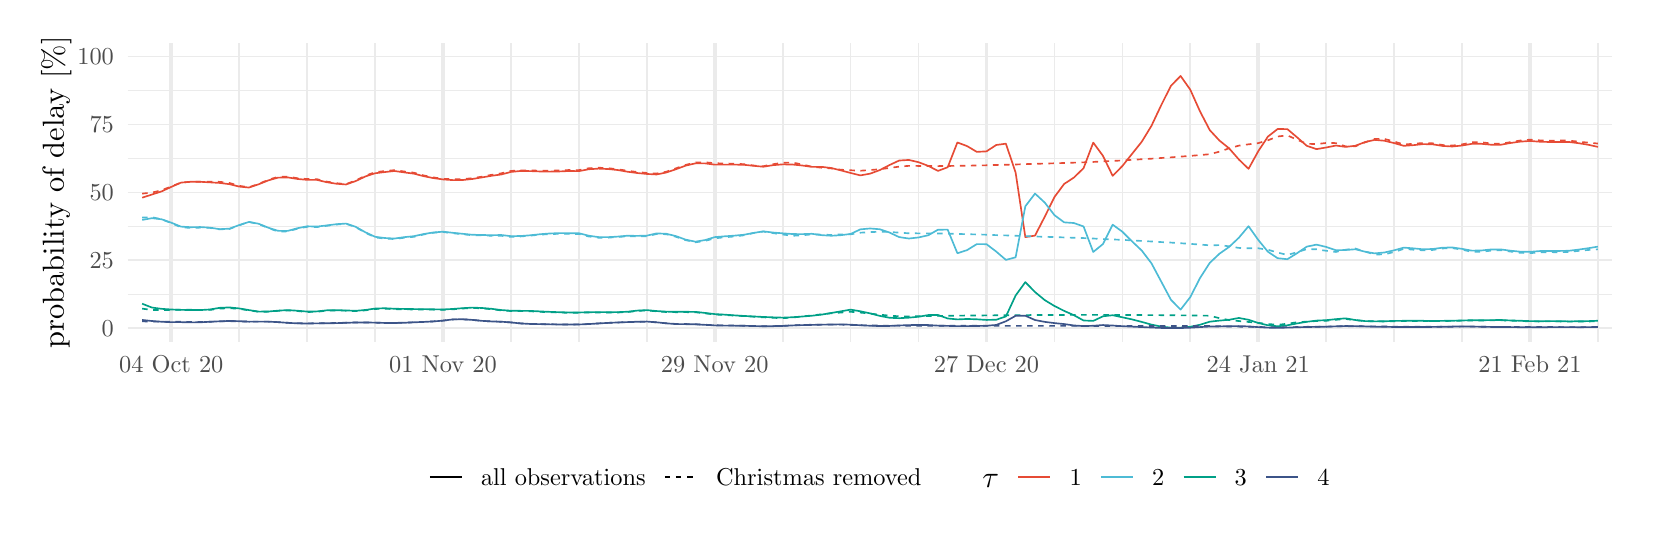
\begin{tikzpicture}[x=1pt,y=1pt]
\definecolor{fillColor}{RGB}{255,255,255}
\path[use as bounding box,fill=fillColor,fill opacity=0.00] (0,0) rectangle (578.16,180.67);
\begin{scope}
\path[clip] ( 36.11, 67.14) rectangle (572.66,175.17);
\definecolor{drawColor}{gray}{0.92}

\path[draw=drawColor,line width= 0.3pt,line join=round] ( 36.11, 84.33) --
	(572.66, 84.33);

\path[draw=drawColor,line width= 0.3pt,line join=round] ( 36.11,108.88) --
	(572.66,108.88);

\path[draw=drawColor,line width= 0.3pt,line join=round] ( 36.11,133.43) --
	(572.66,133.43);

\path[draw=drawColor,line width= 0.3pt,line join=round] ( 36.11,157.99) --
	(572.66,157.99);

\path[draw=drawColor,line width= 0.6pt,line join=round] ( 76.44, 67.14) --
	( 76.44,175.17);

\path[draw=drawColor,line width= 0.6pt,line join=round] (100.99, 67.14) --
	(100.99,175.17);

\path[draw=drawColor,line width= 0.6pt,line join=round] (125.54, 67.14) --
	(125.54,175.17);

\path[draw=drawColor,line width= 0.6pt,line join=round] (174.63, 67.14) --
	(174.63,175.17);

\path[draw=drawColor,line width= 0.6pt,line join=round] (199.18, 67.14) --
	(199.18,175.17);

\path[draw=drawColor,line width= 0.6pt,line join=round] (223.73, 67.14) --
	(223.73,175.17);

\path[draw=drawColor,line width= 0.6pt,line join=round] (272.82, 67.14) --
	(272.82,175.17);

\path[draw=drawColor,line width= 0.6pt,line join=round] (297.37, 67.14) --
	(297.37,175.17);

\path[draw=drawColor,line width= 0.6pt,line join=round] (321.92, 67.14) --
	(321.92,175.17);

\path[draw=drawColor,line width= 0.6pt,line join=round] (371.02, 67.14) --
	(371.02,175.17);

\path[draw=drawColor,line width= 0.6pt,line join=round] (395.56, 67.14) --
	(395.56,175.17);

\path[draw=drawColor,line width= 0.6pt,line join=round] (420.11, 67.14) --
	(420.11,175.17);

\path[draw=drawColor,line width= 0.6pt,line join=round] (469.21, 67.14) --
	(469.21,175.17);

\path[draw=drawColor,line width= 0.6pt,line join=round] (493.76, 67.14) --
	(493.76,175.17);

\path[draw=drawColor,line width= 0.6pt,line join=round] (518.30, 67.14) --
	(518.30,175.17);

\path[draw=drawColor,line width= 0.6pt,line join=round] (567.40, 67.14) --
	(567.40,175.17);

\path[draw=drawColor,line width= 0.6pt,line join=round] ( 36.11, 72.05) --
	(572.66, 72.05);

\path[draw=drawColor,line width= 0.6pt,line join=round] ( 36.11, 96.60) --
	(572.66, 96.60);

\path[draw=drawColor,line width= 0.6pt,line join=round] ( 36.11,121.16) --
	(572.66,121.16);

\path[draw=drawColor,line width= 0.6pt,line join=round] ( 36.11,145.71) --
	(572.66,145.71);

\path[draw=drawColor,line width= 0.6pt,line join=round] ( 36.11,170.26) --
	(572.66,170.26);

\path[draw=drawColor,line width= 1.4pt,line join=round] ( 51.89, 67.14) --
	( 51.89,175.17);

\path[draw=drawColor,line width= 1.4pt,line join=round] (150.08, 67.14) --
	(150.08,175.17);

\path[draw=drawColor,line width= 1.4pt,line join=round] (248.28, 67.14) --
	(248.28,175.17);

\path[draw=drawColor,line width= 1.4pt,line join=round] (346.47, 67.14) --
	(346.47,175.17);

\path[draw=drawColor,line width= 1.4pt,line join=round] (444.66, 67.14) --
	(444.66,175.17);

\path[draw=drawColor,line width= 1.4pt,line join=round] (542.85, 67.14) --
	(542.85,175.17);
\definecolor{drawColor}{RGB}{230,75,53}

\path[draw=drawColor,line width= 0.6pt,line join=round] ( 41.37,119.24) --
	( 44.88,120.37) --
	( 48.39,121.51) --
	( 51.89,123.13) --
	( 55.40,124.68) --
	( 58.91,125.00) --
	( 62.41,124.97) --
	( 65.92,124.77) --
	( 69.43,124.56) --
	( 72.93,124.11) --
	( 76.44,123.25) --
	( 79.95,122.90) --
	( 83.45,124.07) --
	( 86.96,125.49) --
	( 90.47,126.48) --
	( 93.97,126.56) --
	( 97.48,126.00) --
	(100.99,125.68) --
	(104.49,125.67) --
	(108.00,124.84) --
	(111.51,124.28) --
	(115.02,124.01) --
	(118.52,125.24) --
	(122.03,126.90) --
	(125.54,128.06) --
	(129.04,128.49) --
	(132.55,128.88) --
	(136.06,128.37) --
	(139.56,127.92) --
	(143.07,127.01) --
	(146.58,126.32) --
	(150.08,125.83) --
	(153.59,125.59) --
	(157.10,125.61) --
	(160.60,125.98) --
	(164.11,126.55) --
	(167.62,127.15) --
	(171.13,127.62) --
	(174.63,128.54) --
	(178.14,128.89) --
	(181.65,128.84) --
	(185.15,128.71) --
	(188.66,128.66) --
	(192.17,128.72) --
	(195.67,128.87) --
	(199.18,128.83) --
	(202.69,129.50) --
	(206.19,129.73) --
	(209.70,129.59) --
	(213.21,129.23) --
	(216.71,128.62) --
	(220.22,128.15) --
	(223.73,127.81) --
	(227.23,127.62) --
	(230.74,128.33) --
	(234.25,129.51) --
	(237.76,130.82) --
	(241.26,131.63) --
	(244.77,131.63) --
	(248.28,131.17) --
	(251.78,131.17) --
	(255.29,131.19) --
	(258.80,131.12) --
	(262.30,130.76) --
	(265.81,130.42) --
	(269.32,130.98) --
	(272.82,131.27) --
	(276.33,131.22) --
	(279.84,130.87) --
	(283.34,130.38) --
	(286.85,130.38) --
	(290.36,129.96) --
	(293.87,129.09) --
	(297.37,128.16) --
	(300.88,127.29) --
	(304.39,127.91) --
	(307.89,129.20) --
	(311.40,131.02) --
	(314.91,132.66) --
	(318.41,132.87) --
	(321.92,132.06) --
	(325.43,130.72) --
	(328.93,128.91) --
	(332.44,130.23) --
	(335.95,139.19) --
	(339.45,137.88) --
	(342.96,135.79) --
	(346.47,135.97) --
	(349.97,138.27) --
	(353.48,138.75) --
	(356.99,128.30) --
	(360.50,104.99) --
	(364.00,105.53) --
	(367.51,112.35) --
	(371.02,119.47) --
	(374.52,124.19) --
	(378.03,126.49) --
	(381.54,129.89) --
	(385.04,139.14) --
	(388.55,134.36) --
	(392.06,127.13) --
	(395.56,130.67) --
	(399.07,135.08) --
	(402.58,139.47) --
	(406.08,145.21) --
	(409.59,152.64) --
	(413.10,159.64) --
	(416.60,163.22) --
	(420.11,158.25) --
	(423.62,150.42) --
	(427.13,143.67) --
	(430.63,139.89) --
	(434.14,137.06) --
	(437.65,133.05) --
	(441.15,129.66) --
	(444.66,136.01) --
	(448.17,141.33) --
	(451.67,144.05) --
	(455.18,144.01) --
	(458.69,141.05) --
	(462.19,137.98) --
	(465.70,136.78) --
	(469.21,137.37) --
	(472.71,138.08) --
	(476.22,137.59) --
	(479.73,137.99) --
	(483.24,139.33) --
	(486.74,140.12) --
	(490.25,139.81) --
	(493.76,138.97) --
	(497.26,137.97) --
	(500.77,138.22) --
	(504.28,138.60) --
	(507.78,138.50) --
	(511.29,137.93) --
	(514.80,137.73) --
	(518.30,138.08) --
	(521.81,138.69) --
	(525.32,138.70) --
	(528.82,138.37) --
	(532.33,138.37) --
	(535.84,139.00) --
	(539.34,139.49) --
	(542.85,139.73) --
	(546.36,139.46) --
	(549.87,139.36) --
	(553.37,139.36) --
	(556.88,139.37) --
	(560.39,138.93) --
	(563.89,138.36) --
	(567.40,137.59);

\path[draw=drawColor,line width= 0.6pt,dash pattern=on 2pt off 2pt ,line join=round] ( 41.37,120.70) --
	( 44.88,121.07) --
	( 48.39,121.91) --
	( 51.89,123.31) --
	( 55.40,124.69) --
	( 58.91,124.97) --
	( 62.41,125.01) --
	( 65.92,125.00) --
	( 69.43,124.96) --
	( 72.93,124.55) --
	( 76.44,123.52) --
	( 79.95,122.99) --
	( 83.45,124.23) --
	( 86.96,125.68) --
	( 90.47,126.79) --
	( 93.97,126.84) --
	( 97.48,126.26) --
	(100.99,125.97) --
	(104.49,125.93) --
	(108.00,125.06) --
	(111.51,124.48) --
	(115.02,124.13) --
	(118.52,125.46) --
	(122.03,127.18) --
	(125.54,128.44) --
	(129.04,128.86) --
	(132.55,129.18) --
	(136.06,128.70) --
	(139.56,128.26) --
	(143.07,127.28) --
	(146.58,126.56) --
	(150.08,126.04) --
	(153.59,125.90) --
	(157.10,125.90) --
	(160.60,126.28) --
	(164.11,126.82) --
	(167.62,127.49) --
	(171.13,128.04) --
	(174.63,128.90) --
	(178.14,129.12) --
	(181.65,129.08) --
	(185.15,128.99) --
	(188.66,129.00) --
	(192.17,129.06) --
	(195.67,129.23) --
	(199.18,129.20) --
	(202.69,129.86) --
	(206.19,130.07) --
	(209.70,129.90) --
	(213.21,129.49) --
	(216.71,128.97) --
	(220.22,128.51) --
	(223.73,128.18) --
	(227.23,127.95) --
	(230.74,128.61) --
	(234.25,129.84) --
	(237.76,131.08) --
	(241.26,131.96) --
	(244.77,132.02) --
	(248.28,131.70) --
	(251.78,131.58) --
	(255.29,131.53) --
	(258.80,131.33) --
	(262.30,130.85) --
	(265.81,130.61) --
	(269.32,131.33) --
	(272.82,131.86) --
	(276.33,131.93) --
	(279.84,131.25) --
	(283.34,130.42) --
	(286.85,130.08) --
	(290.36,129.81) --
	(293.87,129.34) --
	(297.37,129.14) --
	(300.88,128.98) --
	(304.39,129.22) --
	(307.89,129.51) --
	(311.40,129.97) --
	(314.91,130.46) --
	(318.41,130.74) --
	(321.92,130.71) --
	(325.43,130.67) --
	(328.93,130.65) --
	(332.44,130.69) --
	(335.95,130.76) --
	(339.45,130.80) --
	(342.96,130.87) --
	(346.47,130.93) --
	(349.97,131.06) --
	(353.48,131.13) --
	(356.99,131.23) --
	(360.50,131.36) --
	(364.00,131.47) --
	(367.51,131.56) --
	(371.02,131.66) --
	(374.52,131.77) --
	(378.03,131.89) --
	(381.54,132.00) --
	(385.04,132.15) --
	(388.55,132.36) --
	(392.06,132.51) --
	(395.56,132.69) --
	(399.07,132.92) --
	(402.58,133.13) --
	(406.08,133.33) --
	(409.59,133.58) --
	(413.10,133.80) --
	(416.60,134.07) --
	(420.11,134.34) --
	(423.62,134.63) --
	(427.13,134.95) --
	(430.63,135.86) --
	(434.14,137.08) --
	(437.65,138.04) --
	(441.15,138.52) --
	(444.66,138.95) --
	(448.17,139.98) --
	(451.67,141.34) --
	(455.18,141.75) --
	(458.69,140.19) --
	(462.19,138.72) --
	(465.70,138.60) --
	(469.21,139.00) --
	(472.71,138.96) --
	(476.22,137.77) --
	(479.73,137.78) --
	(483.24,139.23) --
	(486.74,140.48) --
	(490.25,140.46) --
	(493.76,139.54) --
	(497.26,138.43) --
	(500.77,138.73) --
	(504.28,138.99) --
	(507.78,138.87) --
	(511.29,138.26) --
	(514.80,138.06) --
	(518.30,138.49) --
	(521.81,139.24) --
	(525.32,139.24) --
	(528.82,138.83) --
	(532.33,138.68) --
	(535.84,139.32) --
	(539.34,139.89) --
	(542.85,140.20) --
	(546.36,139.95) --
	(549.87,139.81) --
	(553.37,139.89) --
	(556.88,139.86) --
	(560.39,139.48) --
	(563.89,139.12) --
	(567.40,138.80);
\definecolor{drawColor}{RGB}{77,187,213}

\path[draw=drawColor,line width= 0.6pt,line join=round] ( 41.37,111.20) --
	( 44.88,111.83) --
	( 48.39,111.43) --
	( 51.89,110.20) --
	( 55.40,108.78) --
	( 58.91,108.57) --
	( 62.41,108.62) --
	( 65.92,108.40) --
	( 69.43,107.85) --
	( 72.93,108.04) --
	( 76.44,109.35) --
	( 79.95,110.47) --
	( 83.45,109.82) --
	( 86.96,108.38) --
	( 90.47,107.26) --
	( 93.97,107.23) --
	( 97.48,108.20) --
	(100.99,108.90) --
	(104.49,108.79) --
	(108.00,109.20) --
	(111.51,109.65) --
	(115.02,109.88) --
	(118.52,108.70) --
	(122.03,106.73) --
	(125.54,105.10) --
	(129.04,104.66) --
	(132.55,104.47) --
	(136.06,104.97) --
	(139.56,105.32) --
	(143.07,106.09) --
	(146.58,106.67) --
	(150.08,106.94) --
	(153.59,106.55) --
	(157.10,106.19) --
	(160.60,105.84) --
	(164.11,105.76) --
	(167.62,105.67) --
	(171.13,105.75) --
	(174.63,105.33) --
	(178.14,105.38) --
	(181.65,105.65) --
	(185.15,106.03) --
	(188.66,106.30) --
	(192.17,106.43) --
	(195.67,106.40) --
	(199.18,106.40) --
	(202.69,105.50) --
	(206.19,105.00) --
	(209.70,104.97) --
	(213.21,105.17) --
	(216.71,105.49) --
	(220.22,105.43) --
	(223.73,105.52) --
	(227.23,106.32) --
	(230.74,106.20) --
	(234.25,105.35) --
	(237.76,104.07) --
	(241.26,103.34) --
	(244.77,103.92) --
	(248.28,104.99) --
	(251.78,105.27) --
	(255.29,105.51) --
	(258.80,105.84) --
	(262.30,106.50) --
	(265.81,107.07) --
	(269.32,106.64) --
	(272.82,106.36) --
	(276.33,106.10) --
	(279.84,106.06) --
	(283.34,106.19) --
	(286.85,105.70) --
	(290.36,105.48) --
	(293.87,105.69) --
	(297.37,106.13) --
	(300.88,107.79) --
	(304.39,108.11) --
	(307.89,107.83) --
	(311.40,106.65) --
	(314.91,104.99) --
	(318.41,104.48) --
	(321.92,104.86) --
	(325.43,105.66) --
	(328.93,107.66) --
	(332.44,107.69) --
	(335.95, 99.16) --
	(339.45,100.29) --
	(342.96,102.46) --
	(346.47,102.43) --
	(349.97, 99.77) --
	(353.48, 96.76) --
	(356.99, 97.68) --
	(360.50,116.12) --
	(364.00,120.72) --
	(367.51,117.48) --
	(371.02,112.93) --
	(374.52,110.32) --
	(378.03,110.08) --
	(381.54,108.84) --
	(385.04, 99.62) --
	(388.55,102.48) --
	(392.06,109.48) --
	(395.56,106.94) --
	(399.07,103.44) --
	(402.58,100.12) --
	(406.08, 95.52) --
	(409.59, 88.95) --
	(413.10, 82.36) --
	(416.60, 78.78) --
	(420.11, 83.32) --
	(423.62, 90.20) --
	(427.13, 95.66) --
	(430.63, 98.98) --
	(434.14,101.44) --
	(437.65,104.75) --
	(441.15,108.93) --
	(444.66,103.98) --
	(448.17, 99.68) --
	(451.67, 97.37) --
	(455.18, 97.00) --
	(458.69, 99.17) --
	(462.19,101.54) --
	(465.70,102.27) --
	(469.21,101.44) --
	(472.71,100.24) --
	(476.22,100.33) --
	(479.73,100.59) --
	(483.24, 99.72) --
	(486.74, 99.11) --
	(490.25, 99.43) --
	(493.76,100.22) --
	(497.26,101.19) --
	(500.77,100.92) --
	(504.28,100.58) --
	(507.78,100.70) --
	(511.29,101.17) --
	(514.80,101.25) --
	(518.30,100.74) --
	(521.81,100.10) --
	(525.32,100.16) --
	(528.82,100.53) --
	(532.33,100.54) --
	(535.84,100.07) --
	(539.34, 99.73) --
	(542.85, 99.67) --
	(546.36, 99.94) --
	(549.87, 99.98) --
	(553.37, 99.99) --
	(556.88,100.05) --
	(560.39,100.47) --
	(563.89,100.97) --
	(567.40,101.55);

\path[draw=drawColor,line width= 0.6pt,dash pattern=on 2pt off 2pt ,line join=round] ( 41.37,112.04) --
	( 44.88,112.19) --
	( 48.39,111.45) --
	( 51.89,110.03) --
	( 55.40,108.55) --
	( 58.91,108.30) --
	( 62.41,108.41) --
	( 65.92,108.31) --
	( 69.43,107.78) --
	( 72.93,107.94) --
	( 76.44,109.28) --
	( 79.95,110.47) --
	( 83.45,109.72) --
	( 86.96,108.25) --
	( 90.47,107.02) --
	( 93.97,107.05) --
	( 97.48,108.02) --
	(100.99,108.70) --
	(104.49,108.61) --
	(108.00,109.07) --
	(111.51,109.51) --
	(115.02,109.84) --
	(118.52,108.59) --
	(122.03,106.58) --
	(125.54,104.88) --
	(129.04,104.46) --
	(132.55,104.29) --
	(136.06,104.76) --
	(139.56,105.10) --
	(143.07,105.94) --
	(146.58,106.56) --
	(150.08,106.83) --
	(153.59,106.39) --
	(157.10,106.04) --
	(160.60,105.66) --
	(164.11,105.62) --
	(167.62,105.47) --
	(171.13,105.46) --
	(174.63,105.08) --
	(178.14,105.23) --
	(181.65,105.53) --
	(185.15,105.88) --
	(188.66,106.07) --
	(192.17,106.19) --
	(195.67,106.15) --
	(199.18,106.13) --
	(202.69,105.23) --
	(206.19,104.78) --
	(209.70,104.78) --
	(213.21,105.04) --
	(216.71,105.28) --
	(220.22,105.23) --
	(223.73,105.32) --
	(227.23,106.10) --
	(230.74,106.04) --
	(234.25,105.11) --
	(237.76,103.89) --
	(241.26,103.11) --
	(244.77,103.62) --
	(248.28,104.55) --
	(251.78,104.92) --
	(255.29,105.21) --
	(258.80,105.65) --
	(262.30,106.47) --
	(265.81,107.00) --
	(269.32,106.44) --
	(272.82,105.93) --
	(276.33,105.47) --
	(279.84,105.62) --
	(283.34,106.00) --
	(286.85,105.88) --
	(290.36,105.78) --
	(293.87,105.98) --
	(297.37,106.00) --
	(300.88,106.58) --
	(304.39,106.79) --
	(307.89,106.94) --
	(311.40,106.84) --
	(314.91,106.60) --
	(318.41,106.37) --
	(321.92,106.35) --
	(325.43,106.34) --
	(328.93,106.32) --
	(332.44,106.24) --
	(335.95,106.13) --
	(339.45,106.04) --
	(342.96,105.95) --
	(346.47,105.86) --
	(349.97,105.70) --
	(353.48,105.61) --
	(356.99,105.48) --
	(360.50,105.34) --
	(364.00,105.21) --
	(367.51,105.10) --
	(371.02,105.00) --
	(374.52,104.87) --
	(378.03,104.75) --
	(381.54,104.64) --
	(385.04,104.48) --
	(388.55,104.28) --
	(392.06,104.15) --
	(395.56,103.99) --
	(399.07,103.80) --
	(402.58,103.59) --
	(406.08,103.41) --
	(409.59,103.19) --
	(413.10,103.01) --
	(416.60,102.78) --
	(420.11,102.54) --
	(423.62,102.29) --
	(427.13,102.02) --
	(430.63,102.09) --
	(434.14,101.66) --
	(437.65,101.09) --
	(441.15,100.97) --
	(444.66,100.95) --
	(448.17,100.43) --
	(451.67, 99.41) --
	(455.18, 98.55) --
	(458.69, 99.52) --
	(462.19,100.67) --
	(465.70,100.59) --
	(469.21,100.04) --
	(472.71, 99.63) --
	(476.22,100.43) --
	(479.73,100.86) --
	(483.24, 99.77) --
	(486.74, 98.70) --
	(490.25, 98.76) --
	(493.76, 99.63) --
	(497.26,100.74) --
	(500.77,100.43) --
	(504.28,100.21) --
	(507.78,100.36) --
	(511.29,100.89) --
	(514.80,101.01) --
	(518.30,100.47) --
	(521.81, 99.66) --
	(525.32, 99.70) --
	(528.82,100.11) --
	(532.33,100.25) --
	(535.84, 99.76) --
	(539.34, 99.32) --
	(542.85, 99.20) --
	(546.36, 99.46) --
	(549.87, 99.57) --
	(553.37, 99.51) --
	(556.88, 99.63) --
	(560.39,100.01) --
	(563.89,100.34) --
	(567.40,100.58);
\definecolor{drawColor}{RGB}{0,160,135}

\path[draw=drawColor,line width= 0.6pt,line join=round] ( 41.37, 80.92) --
	( 44.88, 79.54) --
	( 48.39, 79.07) --
	( 51.89, 78.83) --
	( 55.40, 78.69) --
	( 58.91, 78.66) --
	( 62.41, 78.62) --
	( 65.92, 78.85) --
	( 69.43, 79.44) --
	( 72.93, 79.58) --
	( 76.44, 79.22) --
	( 79.95, 78.62) --
	( 83.45, 78.07) --
	( 86.96, 78.10) --
	( 90.47, 78.42) --
	( 93.97, 78.61) --
	( 97.48, 78.39) --
	(100.99, 78.08) --
	(104.49, 78.14) --
	(108.00, 78.53) --
	(111.51, 78.58) --
	(115.02, 78.50) --
	(118.52, 78.35) --
	(122.03, 78.66) --
	(125.54, 79.17) --
	(129.04, 79.29) --
	(132.55, 79.10) --
	(136.06, 79.04) --
	(139.56, 78.98) --
	(143.07, 78.97) --
	(146.58, 78.90) --
	(150.08, 78.84) --
	(153.59, 79.03) --
	(157.10, 79.30) --
	(160.60, 79.51) --
	(164.11, 79.38) --
	(167.62, 79.08) --
	(171.13, 78.63) --
	(174.63, 78.39) --
	(178.14, 78.35) --
	(181.65, 78.32) --
	(185.15, 78.14) --
	(188.66, 77.98) --
	(192.17, 77.85) --
	(195.67, 77.77) --
	(199.18, 77.76) --
	(202.69, 77.85) --
	(206.19, 77.89) --
	(209.70, 77.86) --
	(213.21, 77.87) --
	(216.71, 78.02) --
	(220.22, 78.43) --
	(223.73, 78.61) --
	(227.23, 78.27) --
	(230.74, 78.06) --
	(234.25, 77.99) --
	(237.76, 78.00) --
	(241.26, 77.97) --
	(244.77, 77.59) --
	(248.28, 77.17) --
	(251.78, 76.97) --
	(255.29, 76.72) --
	(258.80, 76.51) --
	(262.30, 76.31) --
	(265.81, 76.14) --
	(269.32, 76.00) --
	(272.82, 75.89) --
	(276.33, 76.03) --
	(279.84, 76.29) --
	(283.34, 76.58) --
	(286.85, 76.98) --
	(290.36, 77.57) --
	(293.87, 78.18) --
	(297.37, 78.78) --
	(300.88, 78.19) --
	(304.39, 77.44) --
	(307.89, 76.52) --
	(311.40, 75.85) --
	(314.91, 75.69) --
	(318.41, 75.88) --
	(321.92, 76.22) --
	(325.43, 76.82) --
	(328.93, 76.85) --
	(332.44, 75.59) --
	(335.95, 75.25) --
	(339.45, 75.41) --
	(342.96, 75.29) --
	(346.47, 75.06) --
	(349.97, 75.13) --
	(353.48, 76.32) --
	(356.99, 83.88) --
	(360.50, 88.72) --
	(364.00, 85.14) --
	(367.51, 82.23) --
	(371.02, 80.09) --
	(374.52, 78.33) --
	(378.03, 76.78) --
	(381.54, 74.86) --
	(385.04, 74.71) --
	(388.55, 76.37) --
	(392.06, 76.77) --
	(395.56, 76.01) --
	(399.07, 75.25) --
	(402.58, 74.34) --
	(406.08, 73.37) --
	(409.59, 72.65) --
	(413.10, 72.28) --
	(416.60, 72.28) --
	(420.11, 72.59) --
	(423.62, 73.32) --
	(427.13, 74.42) --
	(430.63, 74.82) --
	(434.14, 75.12) --
	(437.65, 75.77) --
	(441.15, 75.12) --
	(444.66, 73.96) --
	(448.17, 73.13) --
	(451.67, 72.76) --
	(455.18, 73.12) --
	(458.69, 73.80) --
	(462.19, 74.38) --
	(465.70, 74.82) --
	(469.21, 74.97) --
	(472.71, 75.34) --
	(476.22, 75.64) --
	(479.73, 75.03) --
	(483.24, 74.64) --
	(486.74, 74.55) --
	(490.25, 74.57) --
	(493.76, 74.72) --
	(497.26, 74.74) --
	(500.77, 74.79) --
	(504.28, 74.74) --
	(507.78, 74.68) --
	(511.29, 74.73) --
	(514.80, 74.77) --
	(518.30, 74.86) --
	(521.81, 74.95) --
	(525.32, 74.96) --
	(528.82, 74.99) --
	(532.33, 75.03) --
	(535.84, 74.87) --
	(539.34, 74.77) --
	(542.85, 74.63) --
	(546.36, 74.60) --
	(549.87, 74.63) --
	(553.37, 74.60) --
	(556.88, 74.54) --
	(560.39, 74.57) --
	(563.89, 74.63) --
	(567.40, 74.76);

\path[draw=drawColor,line width= 0.6pt,dash pattern=on 2pt off 2pt ,line join=round] ( 41.37, 79.14) --
	( 44.88, 78.67) --
	( 48.39, 78.63) --
	( 51.89, 78.69) --
	( 55.40, 78.76) --
	( 58.91, 78.80) --
	( 62.41, 78.67) --
	( 65.92, 78.69) --
	( 69.43, 79.15) --
	( 72.93, 79.31) --
	( 76.44, 79.06) --
	( 79.95, 78.52) --
	( 83.45, 78.01) --
	( 86.96, 78.05) --
	( 90.47, 78.34) --
	( 93.97, 78.49) --
	( 97.48, 78.27) --
	(100.99, 77.93) --
	(104.49, 78.01) --
	(108.00, 78.39) --
	(111.51, 78.48) --
	(115.02, 78.40) --
	(118.52, 78.23) --
	(122.03, 78.53) --
	(125.54, 79.02) --
	(129.04, 79.12) --
	(132.55, 78.96) --
	(136.06, 78.91) --
	(139.56, 78.83) --
	(143.07, 78.84) --
	(146.58, 78.77) --
	(150.08, 78.73) --
	(153.59, 78.89) --
	(157.10, 79.18) --
	(160.60, 79.39) --
	(164.11, 79.25) --
	(167.62, 78.94) --
	(171.13, 78.50) --
	(174.63, 78.28) --
	(178.14, 78.25) --
	(181.65, 78.18) --
	(185.15, 77.99) --
	(188.66, 77.85) --
	(192.17, 77.73) --
	(195.67, 77.63) --
	(199.18, 77.64) --
	(202.69, 77.74) --
	(206.19, 77.77) --
	(209.70, 77.74) --
	(213.21, 77.75) --
	(216.71, 77.90) --
	(220.22, 78.31) --
	(223.73, 78.50) --
	(227.23, 78.17) --
	(230.74, 77.92) --
	(234.25, 77.86) --
	(237.76, 77.87) --
	(241.26, 77.84) --
	(244.77, 77.44) --
	(248.28, 77.02) --
	(251.78, 76.86) --
	(255.29, 76.64) --
	(258.80, 76.46) --
	(262.30, 76.24) --
	(265.81, 76.01) --
	(269.32, 75.83) --
	(272.82, 75.70) --
	(276.33, 75.92) --
	(279.84, 76.31) --
	(283.34, 76.69) --
	(286.85, 77.09) --
	(290.36, 77.47) --
	(293.87, 77.73) --
	(297.37, 78.01) --
	(300.88, 77.72) --
	(304.39, 77.35) --
	(307.89, 76.96) --
	(311.40, 76.61) --
	(314.91, 76.37) --
	(318.41, 76.35) --
	(321.92, 76.41) --
	(325.43, 76.46) --
	(328.93, 76.51) --
	(332.44, 76.55) --
	(335.95, 76.59) --
	(339.45, 76.65) --
	(342.96, 76.67) --
	(346.47, 76.70) --
	(349.97, 76.73) --
	(353.48, 76.76) --
	(356.99, 76.79) --
	(360.50, 76.80) --
	(364.00, 76.83) --
	(367.51, 76.84) --
	(371.02, 76.85) --
	(374.52, 76.87) --
	(378.03, 76.88) --
	(381.54, 76.88) --
	(385.04, 76.89) --
	(388.55, 76.88) --
	(392.06, 76.87) --
	(395.56, 76.85) --
	(399.07, 76.82) --
	(402.58, 76.82) --
	(406.08, 76.80) --
	(409.59, 76.78) --
	(413.10, 76.74) --
	(416.60, 76.71) --
	(420.11, 76.68) --
	(423.62, 76.64) --
	(427.13, 76.59) --
	(430.63, 75.69) --
	(434.14, 75.00) --
	(437.65, 74.66) --
	(441.15, 74.33) --
	(444.66, 74.00) --
	(448.17, 73.59) --
	(451.67, 73.29) --
	(455.18, 73.69) --
	(458.69, 74.22) --
	(462.19, 74.45) --
	(465.70, 74.66) --
	(469.21, 74.75) --
	(472.71, 75.11) --
	(476.22, 75.41) --
	(479.73, 74.98) --
	(483.24, 74.67) --
	(486.74, 74.56) --
	(490.25, 74.51) --
	(493.76, 74.61) --
	(497.26, 74.63) --
	(500.77, 74.68) --
	(504.28, 74.64) --
	(507.78, 74.61) --
	(511.29, 74.68) --
	(514.80, 74.72) --
	(518.30, 74.81) --
	(521.81, 74.88) --
	(525.32, 74.87) --
	(528.82, 74.90) --
	(532.33, 74.94) --
	(535.84, 74.79) --
	(539.34, 74.69) --
	(542.85, 74.54) --
	(546.36, 74.52) --
	(549.87, 74.55) --
	(553.37, 74.53) --
	(556.88, 74.46) --
	(560.39, 74.48) --
	(563.89, 74.51) --
	(567.40, 74.57);
\definecolor{drawColor}{RGB}{60,84,136}

\path[draw=drawColor,line width= 0.6pt,line join=round] ( 41.37, 75.05) --
	( 44.88, 74.67) --
	( 48.39, 74.41) --
	( 51.89, 74.26) --
	( 55.40, 74.26) --
	( 58.91, 74.18) --
	( 62.41, 74.21) --
	( 65.92, 74.40) --
	( 69.43, 74.57) --
	( 72.93, 74.69) --
	( 76.44, 74.60) --
	( 79.95, 74.43) --
	( 83.45, 74.46) --
	( 86.96, 74.44) --
	( 90.47, 74.26) --
	( 93.97, 74.01) --
	( 97.48, 73.82) --
	(100.99, 73.76) --
	(104.49, 73.82) --
	(108.00, 73.85) --
	(111.51, 73.90) --
	(115.02, 74.02) --
	(118.52, 74.13) --
	(122.03, 74.13) --
	(125.54, 74.09) --
	(129.04, 73.97) --
	(132.55, 73.96) --
	(136.06, 74.03) --
	(139.56, 74.20) --
	(143.07, 74.34) --
	(146.58, 74.52) --
	(150.08, 74.81) --
	(153.59, 75.25) --
	(157.10, 75.30) --
	(160.60, 75.08) --
	(164.11, 74.73) --
	(167.62, 74.52) --
	(171.13, 74.42) --
	(174.63, 74.16) --
	(178.14, 73.79) --
	(181.65, 73.61) --
	(185.15, 73.54) --
	(188.66, 73.47) --
	(192.17, 73.42) --
	(195.67, 73.38) --
	(199.18, 73.42) --
	(202.69, 73.56) --
	(206.19, 73.79) --
	(209.70, 73.99) --
	(213.21, 74.15) --
	(216.71, 74.28) --
	(220.22, 74.41) --
	(223.73, 74.47) --
	(227.23, 74.21) --
	(230.74, 73.83) --
	(234.25, 73.57) --
	(237.76, 73.53) --
	(241.26, 73.47) --
	(244.77, 73.28) --
	(248.28, 73.09) --
	(251.78, 73.01) --
	(255.29, 72.99) --
	(258.80, 72.95) --
	(262.30, 72.84) --
	(265.81, 72.78) --
	(269.32, 72.80) --
	(272.82, 72.89) --
	(276.33, 73.07) --
	(279.84, 73.19) --
	(283.34, 73.26) --
	(286.85, 73.35) --
	(290.36, 73.41) --
	(293.87, 73.46) --
	(297.37, 73.34) --
	(300.88, 73.14) --
	(304.39, 72.96) --
	(307.89, 72.86) --
	(311.40, 72.89) --
	(314.91, 73.06) --
	(318.41, 73.18) --
	(321.92, 73.27) --
	(325.43, 73.21) --
	(328.93, 73.00) --
	(332.44, 72.91) --
	(335.95, 72.82) --
	(339.45, 72.83) --
	(342.96, 72.87) --
	(346.47, 72.96) --
	(349.97, 73.24) --
	(353.48, 74.58) --
	(356.99, 76.55) --
	(360.50, 76.58) --
	(364.00, 75.03) --
	(367.51, 74.36) --
	(371.02, 73.92) --
	(374.52, 73.57) --
	(378.03, 73.07) --
	(381.54, 72.83) --
	(385.04, 72.95) --
	(388.55, 73.21) --
	(392.06, 73.04) --
	(395.56, 72.80) --
	(399.07, 72.64) --
	(402.58, 72.48) --
	(406.08, 72.32) --
	(409.59, 72.17) --
	(413.10, 72.12) --
	(416.60, 72.14) --
	(420.11, 72.25) --
	(423.62, 72.48) --
	(427.13, 72.67) --
	(430.63, 72.72) --
	(434.14, 72.80) --
	(437.65, 72.84) --
	(441.15, 72.71) --
	(444.66, 72.46) --
	(448.17, 72.27) --
	(451.67, 72.23) --
	(455.18, 72.28) --
	(458.69, 72.40) --
	(462.19, 72.52) --
	(465.70, 72.55) --
	(469.21, 72.63) --
	(472.71, 72.75) --
	(476.22, 72.85) --
	(479.73, 72.81) --
	(483.24, 72.72) --
	(486.74, 72.63) --
	(490.25, 72.60) --
	(493.76, 72.51) --
	(497.26, 72.51) --
	(500.77, 72.48) --
	(504.28, 72.50) --
	(507.78, 72.54) --
	(511.29, 72.58) --
	(514.80, 72.66) --
	(518.30, 72.73) --
	(521.81, 72.68) --
	(525.32, 72.60) --
	(528.82, 72.53) --
	(532.33, 72.48) --
	(535.84, 72.48) --
	(539.34, 72.43) --
	(542.85, 72.39) --
	(546.36, 72.42) --
	(549.87, 72.45) --
	(553.37, 72.47) --
	(556.88, 72.47) --
	(560.39, 72.44) --
	(563.89, 72.46) --
	(567.40, 72.51);

\path[draw=drawColor,line width= 0.6pt,dash pattern=on 2pt off 2pt ,line join=round] ( 41.37, 74.54) --
	( 44.88, 74.48) --
	( 48.39, 74.42) --
	( 51.89, 74.39) --
	( 55.40, 74.42) --
	( 58.91, 74.34) --
	( 62.41, 74.32) --
	( 65.92, 74.42) --
	( 69.43, 74.52) --
	( 72.93, 74.62) --
	( 76.44, 74.56) --
	( 79.95, 74.44) --
	( 83.45, 74.46) --
	( 86.96, 74.44) --
	( 90.47, 74.26) --
	( 93.97, 74.03) --
	( 97.48, 73.87) --
	(100.99, 73.81) --
	(104.49, 73.86) --
	(108.00, 73.89) --
	(111.51, 73.95) --
	(115.02, 74.05) --
	(118.52, 74.14) --
	(122.03, 74.12) --
	(125.54, 74.09) --
	(129.04, 73.98) --
	(132.55, 73.99) --
	(136.06, 74.06) --
	(139.56, 74.22) --
	(143.07, 74.36) --
	(146.58, 74.53) --
	(150.08, 74.82) --
	(153.59, 75.24) --
	(157.10, 75.29) --
	(160.60, 75.08) --
	(164.11, 74.73) --
	(167.62, 74.52) --
	(171.13, 74.41) --
	(174.63, 74.16) --
	(178.14, 73.81) --
	(181.65, 73.62) --
	(185.15, 73.56) --
	(188.66, 73.49) --
	(192.17, 73.44) --
	(195.67, 73.42) --
	(199.18, 73.45) --
	(202.69, 73.59) --
	(206.19, 73.80) --
	(209.70, 73.99) --
	(213.21, 74.14) --
	(216.71, 74.26) --
	(220.22, 74.37) --
	(223.73, 74.41) --
	(227.23, 74.19) --
	(230.74, 73.85) --
	(234.25, 73.61) --
	(237.76, 73.57) --
	(241.26, 73.51) --
	(244.77, 73.33) --
	(248.28, 73.14) --
	(251.78, 73.06) --
	(255.29, 73.03) --
	(258.80, 72.98) --
	(262.30, 72.86) --
	(265.81, 72.80) --
	(269.32, 72.82) --
	(272.82, 72.92) --
	(276.33, 73.10) --
	(279.84, 73.24) --
	(283.34, 73.31) --
	(286.85, 73.36) --
	(290.36, 73.36) --
	(293.87, 73.37) --
	(297.37, 73.27) --
	(300.88, 73.13) --
	(304.39, 73.05) --
	(307.89, 73.02) --
	(311.40, 73.00) --
	(314.91, 72.99) --
	(318.41, 72.95) --
	(321.92, 72.95) --
	(325.43, 72.94) --
	(328.93, 72.94) --
	(332.44, 72.94) --
	(335.95, 72.93) --
	(339.45, 72.93) --
	(342.96, 72.93) --
	(346.47, 72.92) --
	(349.97, 72.92) --
	(353.48, 72.92) --
	(356.99, 72.92) --
	(360.50, 72.91) --
	(364.00, 72.91) --
	(367.51, 72.91) --
	(371.02, 72.90) --
	(374.52, 72.90) --
	(378.03, 72.90) --
	(381.54, 72.90) --
	(385.04, 72.89) --
	(388.55, 72.89) --
	(392.06, 72.89) --
	(395.56, 72.88) --
	(399.07, 72.88) --
	(402.58, 72.88) --
	(406.08, 72.87) --
	(409.59, 72.87) --
	(413.10, 72.87) --
	(416.60, 72.86) --
	(420.11, 72.86) --
	(423.62, 72.86) --
	(427.13, 72.85) --
	(430.63, 72.77) --
	(434.14, 72.68) --
	(437.65, 72.63) --
	(441.15, 72.59) --
	(444.66, 72.52) --
	(448.17, 72.42) --
	(451.67, 72.37) --
	(455.18, 72.42) --
	(458.69, 72.49) --
	(462.19, 72.57) --
	(465.70, 72.57) --
	(469.21, 72.62) --
	(472.71, 72.71) --
	(476.22, 72.81) --
	(479.73, 72.79) --
	(483.24, 72.74) --
	(486.74, 72.68) --
	(490.25, 72.68) --
	(493.76, 72.64) --
	(497.26, 72.62) --
	(500.77, 72.58) --
	(504.28, 72.57) --
	(507.78, 72.58) --
	(511.29, 72.59) --
	(514.80, 72.62) --
	(518.30, 72.65) --
	(521.81, 72.64) --
	(525.32, 72.61) --
	(528.82, 72.57) --
	(532.33, 72.55) --
	(535.84, 72.55) --
	(539.34, 72.51) --
	(542.85, 72.48) --
	(546.36, 72.48) --
	(549.87, 72.49) --
	(553.37, 72.48) --
	(556.88, 72.46) --
	(560.39, 72.44) --
	(563.89, 72.45) --
	(567.40, 72.47);
\end{scope}
\begin{scope}
\path[clip] (  0.00,  0.00) rectangle (578.16,180.67);
\definecolor{drawColor}{gray}{0.30}

\node[text=drawColor,anchor=base east,inner sep=0pt, outer sep=0pt, scale=  0.88] at ( 31.16, 69.02) {0};

\node[text=drawColor,anchor=base east,inner sep=0pt, outer sep=0pt, scale=  0.88] at ( 31.16, 93.57) {25};

\node[text=drawColor,anchor=base east,inner sep=0pt, outer sep=0pt, scale=  0.88] at ( 31.16,118.13) {50};

\node[text=drawColor,anchor=base east,inner sep=0pt, outer sep=0pt, scale=  0.88] at ( 31.16,142.68) {75};

\node[text=drawColor,anchor=base east,inner sep=0pt, outer sep=0pt, scale=  0.88] at ( 31.16,167.23) {100};
\end{scope}
\begin{scope}
\path[clip] (  0.00,  0.00) rectangle (578.16,180.67);
\definecolor{drawColor}{gray}{0.30}

\node[text=drawColor,anchor=base,inner sep=0pt, outer sep=0pt, scale=  0.88] at ( 51.89, 56.13) {04 Oct 20};

\node[text=drawColor,anchor=base,inner sep=0pt, outer sep=0pt, scale=  0.88] at (150.08, 56.13) {01 Nov 20};

\node[text=drawColor,anchor=base,inner sep=0pt, outer sep=0pt, scale=  0.88] at (248.28, 56.13) {29 Nov 20};

\node[text=drawColor,anchor=base,inner sep=0pt, outer sep=0pt, scale=  0.88] at (346.47, 56.13) {27 Dec 20};

\node[text=drawColor,anchor=base,inner sep=0pt, outer sep=0pt, scale=  0.88] at (444.66, 56.13) {24 Jan 21};

\node[text=drawColor,anchor=base,inner sep=0pt, outer sep=0pt, scale=  0.88] at (542.85, 56.13) {21 Feb 21};
\end{scope}
\begin{scope}
\path[clip] (  0.00,  0.00) rectangle (578.16,180.67);
\definecolor{drawColor}{RGB}{0,0,0}

\node[text=drawColor,rotate= 90.00,anchor=base,inner sep=0pt, outer sep=0pt, scale=  1.10] at ( 13.08,121.16) {probability of delay [\%]};
\end{scope}
\begin{scope}
\path[clip] (  0.00,  0.00) rectangle (578.16,180.67);
\definecolor{drawColor}{RGB}{0,0,0}

\path[draw=drawColor,line width= 0.6pt,line join=round] (145.29, 18.23) -- (156.86, 18.23);
\end{scope}
\begin{scope}
\path[clip] (  0.00,  0.00) rectangle (578.16,180.67);
\definecolor{drawColor}{RGB}{0,0,0}

\path[draw=drawColor,line width= 0.6pt,dash pattern=on 2pt off 2pt ,line join=round] (230.25, 18.23) -- (241.82, 18.23);
\end{scope}
\begin{scope}
\path[clip] (  0.00,  0.00) rectangle (578.16,180.67);
\definecolor{drawColor}{RGB}{0,0,0}

\node[text=drawColor,anchor=base west,inner sep=0pt, outer sep=0pt, scale=  0.88] at (163.80, 15.20) {all observations};
\end{scope}
\begin{scope}
\path[clip] (  0.00,  0.00) rectangle (578.16,180.67);
\definecolor{drawColor}{RGB}{0,0,0}

\node[text=drawColor,anchor=base west,inner sep=0pt, outer sep=0pt, scale=  0.88] at (248.76, 15.20) {Christmas removed};
\end{scope}
\begin{scope}
\path[clip] (  0.00,  0.00) rectangle (578.16,180.67);
\definecolor{drawColor}{RGB}{0,0,0}

\node[text=drawColor,anchor=base west,inner sep=0pt, outer sep=0pt, scale=  1.10] at (344.96, 14.44) {$\tau$};
\end{scope}
\begin{scope}
\path[clip] (  0.00,  0.00) rectangle (578.16,180.67);
\definecolor{drawColor}{RGB}{230,75,53}

\path[draw=drawColor,line width= 0.6pt,line join=round] (357.96, 18.23) -- (369.52, 18.23);
\end{scope}
\begin{scope}
\path[clip] (  0.00,  0.00) rectangle (578.16,180.67);
\definecolor{drawColor}{RGB}{77,187,213}

\path[draw=drawColor,line width= 0.6pt,line join=round] (387.81, 18.23) -- (399.37, 18.23);
\end{scope}
\begin{scope}
\path[clip] (  0.00,  0.00) rectangle (578.16,180.67);
\definecolor{drawColor}{RGB}{0,160,135}

\path[draw=drawColor,line width= 0.6pt,line join=round] (417.66, 18.23) -- (429.23, 18.23);
\end{scope}
\begin{scope}
\path[clip] (  0.00,  0.00) rectangle (578.16,180.67);
\definecolor{drawColor}{RGB}{60,84,136}

\path[draw=drawColor,line width= 0.6pt,line join=round] (447.52, 18.23) -- (459.08, 18.23);
\end{scope}
\begin{scope}
\path[clip] (  0.00,  0.00) rectangle (578.16,180.67);
\definecolor{drawColor}{RGB}{0,0,0}

\node[text=drawColor,anchor=base west,inner sep=0pt, outer sep=0pt, scale=  0.88] at (376.47, 15.20) {1};
\end{scope}
\begin{scope}
\path[clip] (  0.00,  0.00) rectangle (578.16,180.67);
\definecolor{drawColor}{RGB}{0,0,0}

\node[text=drawColor,anchor=base west,inner sep=0pt, outer sep=0pt, scale=  0.88] at (406.32, 15.20) {2};
\end{scope}
\begin{scope}
\path[clip] (  0.00,  0.00) rectangle (578.16,180.67);
\definecolor{drawColor}{RGB}{0,0,0}

\node[text=drawColor,anchor=base west,inner sep=0pt, outer sep=0pt, scale=  0.88] at (436.17, 15.20) {3};
\end{scope}
\begin{scope}
\path[clip] (  0.00,  0.00) rectangle (578.16,180.67);
\definecolor{drawColor}{RGB}{0,0,0}

\node[text=drawColor,anchor=base west,inner sep=0pt, outer sep=0pt, scale=  0.88] at (466.03, 15.20) {4};
\end{scope}
\end{tikzpicture}
%
    }
    \caption{Importance sampling estimates of conditional expectation $\E \left( p_{t, \tau} | Y \right)$ for the two Christmas models. }
    \label{fig:christmas_delay_probs}
\end{figure}

\subsection{Discussion}
% extension: for true dealing with week-day effect, use information on symptom onset date
% extension: death data, both for forecasting and improving estimation
% extension: longer delays
% extension: keep number of cases in missing scenario constant
% extension: dark figure, w/deaths
% extension: weekday effects normalized like delays
\section{Regional growth factor model}%
\label{sec:regional_growth_factor_model}

\subsection{Context}

Modeling the epidemics spread on a regional level allows us to differentiate between localized and global outbreaks, such as the one in June 2020, highlighted in \Cref{fig:cases_germany}. Additionally, regional level prediction and growth factors are of interest on their own, because \acrshortpl{npi} are enforced on the regional level. Moreover, having access to the spread on the regional level enables, e.g., regression of the growth rate against regional covariates, which in turn sheds light on which factors drive the epidemic.

Instead of modeling the number of cases per day and with delay as we did in \Cref{sec:model_reporting_delay}, we will now model the total number of cases reported within one week for every county in Germany. Here we assume that a sufficient time period has passed, i.e. several days, see \Cref{fig:reporting_delays_cases}, such that the total number of cases is known sufficiently well. This weekly approach has several advantages: First, aggregating over the weekly data gets rid of the weekday effect, at the expense of a lower time resolution. Second, if we are interested in a retrospective analysis, it is sensible to assume all cases have been reported already, so we can avoid modeling the reporting delays. 

However, modeling cases on the regional level comes with its own challenges, as we have to take care of accounting for the spatial spread, as well as an exchange between regions, cf. \Cref{sec:dessiderata}. 


% want regional level predictions / growth factors
% Toennies outbreak
% for small regions, have to consider exchange of cases as well

\subsection{Model}
Similar to the last section, we start by modeling the evolution of cases in time. We now have incidences $I_{t,r}$ reported for reporting date $t$ and region $r$, where there are a total of $R$ regions. 
\todo{comment on Gebietsreform in 2021 (?)}
Again, we model the evolution of cases by 
\begin{align}
    \label{eq:log-growth-regional-model}
    \log I_{t + 1, r} \approx \log I_{t + 1, r} + \log \rho_{t + 1, r}
\end{align}
where $\rho_{t+1, r}$ is the weekly growth factor in region $r$. Now we deviate from the previous model and model 
$$
    \log \rho_{t, r} = \overline{\log \rho}_{t} + u_{t, r},
$$
where $\overline{\log\rho}_{t}$ is the average growth rate and $u_{t,r}$ is the difference between the growth rate in region $r$ and the country wide average. 
We will model $u_{t,r}, r = 1, \dots, R$ to be jointly Gaussian, but correlated, which will enable us to model regional dependencies. To motivate our choice for the covariance structure, let us consider how cases are transferred between regions first.

As we are modeling cases on a regional level, we have to account for an exchange of cases as well. To illustrate our approach, suppose that we have for region $r$ $S^{r}$ many secondary cases generated where the primary case belongs to region $r$, but the secondary case may belong to another region $r'$. Here \glqq{}belonging to\grqq{} signifies that the case is reported in that region, which means that the infectee has registered their center of living to be in this region. Denote by $p_{r,r'}$ the fraction of such cases and set $p_{r,r} = 1 - \sum_{r' \neq r} p_{r,r'}$. 

Under these assumptions, the newly reported cases in region $r$ are 
$$
    \tilde S^{r} = \sum_{r'} p_{r',r} S^{r'} = (P^{T}S)_{r}
$$
for $ P = \left( p_{r, r'} \right)_{r,r' = 1, \dots, R}$. Assuming now that $S^{r}, r= 1, \dots, R$ are random and i.i.d. with variance $\sigma^{2}_S$, we have 
$$
    \cov \left( \tilde S\right) = \cov \left( P^{T}S, P^{T}S \right) = \sigma^{2}_SP^{T}P.
$$

However, modeling the correlation of newly reported cases turns out to be difficult: the cases will surely be modeled by a Poisson or Negative Binomial distribution, so we would have to decide on a copula to introduce this dependency structure. While this is feasible in principle, we opt for an easier way. Instead of modeling correlated incidences $I_{t + 1, r}$, we model correlated growth rates $\log \rho_{t + 1, r}$, by taking $\cov \left( u_{t} \right)$ to be $\sigma^{2}_SP^{T}P$. By \Cref{eq:log-growth-regional-model}, conditional on $I_{t,r}$, this also captures regional correlation, without having to specify an involved joint distribution for the incidences.

As elaborated in \Cref{sec:dessiderata}, we want the regional effects $u_{t,r}$ to be both flexible, but also, in some sense, stable over time. Thus, it makes sense to model $u_{t}$ as a stationary process in time. The simplest, non-trivial, stationary process is a vector-autoregressive process 
$$
    u_{t + 1} = \alpha u_{t} + \varepsilon_{t + 1, u}
$$
where $\alpha \in (-1, 1)$ and $\varepsilon_{t + 1,u} \sim \mathcal N(0, \Gamma)$, where $\Gamma$ is a positive definite matrix. By the above discussion, we set $\Gamma = (1-\alpha^{2}) \sigma^{2}_{S}P^{T}P$ so that the stationary distribution of $u_{t}, t = 0, \dots, n$  is $\mathcal N(0, \sigma^{2}_SP^{T}P)$. 

To setup our \acrshort{ssm}, let $X_{t} = \left( \overline{\log \rho_{t + 1}}, u_{t, 1}, \dots, u_{t, R} \right)^{T} \in \R^{R + 1}$. For the observations, we let $Y_{t} = \left( I_{t, 1}, \dots, I_{t, R} \right)^{T}$, the number of cases observed in regions $1, \dots, R$ in the $t$-th week. 

We then model the number of cases at time $t + 1$ in region $r$, $I_{t+1, r}$ to follow a negative binomial distribution, conditional on the states $X_{t}$ to be
$$
    I_{t+1,r} | I_{t}, \overline{\log\rho}_{t}, u_{t,r} \sim \nbinom \left( \overline{\rho}_{t}\exp(u_{t,r})P^{T}I_t, r\right),
$$
conditionally independent. While the previous observations $I_{t}$ are now conditioned on as well, recall from our discussion in the beginning of \Cref{cha:state_space_models}, that this is not problematic.

To fully specify the model, we have to provide the transfer probabilities $p_{r,r'}$. For these, we use official data by Germany's federal employment agency on commuters \todo{ref}. From these data, we calculate $q_{r,r'}$, the fraction of socially insured employees that have their center of life in region $r$, but are registered to work in region $r'$. As this is only a crude approximation to the actual exchange between regions, we let 
$$
    p_{r,r'} \propto \bar q + (1- \bar q) \frac{q_{r,r'}}{\sum_{r'' \neq r'} q_{r,r''} + C q_{r,r}}
$$
where we interpret $\bar q$ as a constant socket of exchange between regions and $C \geq 1$ as an additional proportion of stay at home inhabitants that are not captured by $q_{r,r}$, e.g. elderly or children. 

Thus, our final model is parameterized by
$$
    \theta = \left( \log \sigma^{2}_S, \operatorname{logit} \alpha, \log (C - 1), \logit \bar q, \log \sigma^{2}_{\overline{\log \rho}}, \log r\right),
$$
where chose a parametrization that is unconstrained. The model has a linear signal 
$$
    S_{t} = \left(\log \rho_{t} + u_{t,r}\right)_{r = 1, \dots, R},
$$
which makes inference fast, as the approximating \acrshort{glssm} in the \acrshort{eis} method only requires $\mathcal O(n\,R)$ many parameters. Again, we use \acrshort{mle} to estimate $\theta$, using the methods from \Cref{sec:maximum_likelihood_estimation}.

\subsection{Results}

\begin{itemize}
    \item fit model by MLE + show inference for Toennies outbreak, interpret covariance matrix estimates
    \item predict incidences on regional level and show that we outperform simple Poisson / NB baseline that only uses a single region
    \item maybe: perform predictions for 1-4 weeks ahead, compare to regional FCH
\end{itemize}

\subsection{Discussion}

\todo{consider Armbruster2024Networkbased, Armillotta2023Inference}
\section{Nowcasting hospitalizations}%
\label{sec:nowcasting_hospitalizations}
\todo{compare SSM predictions to FCH submissions}
\subsection{Context}
Judging the severity of the COVID-19 epidemic has been an ongoing challenge since its inception. As immunization against COVID-19 rose, strict enforcement of social distancing rules eased and testing regimes became less strict, case incidences became a less reliable and harder to interpret indicator of epidemic severity. Instead more direct indicators of morbidity, such as the number of deaths and ICU admissions and occupancy have come to the fore. But these indicators are late due to the substantial delays between infection and occurence. An alternative indicator that captures the morbidity caused by COVID-19 but is earlier than the others is the number of hospitalisations of positive COVID-19
cases.

While hospitalisations occur earlier, they still come with substantial delay between the infection and subsequent admission to hospital. Additional difficulties arise due to delays in reporting, i.e.~the time it takes until the hospital reports the new case to the national health authorities. The problem of accounting for delays in reporting for occurred, but not yet reported events has been termed \textbf{nowcasting}, i.e.~forecasting of the indicator at time ``now''. Predicting the number of hospitalisations is thus a mixture of both forecasting --- which reported COVID-19 cases will end up in the hospital --- and nowcasting --- which cases have yet to be reported --- and we will use the term nowcasting in this paper to mean this predictive mixture. In this section we focus on the situation in Germany where data on hospitalisations has been available since April 2021 provided by the German federal health care authorithy, the \gls{rki}, via Github \citep{RobertKoch-Institut2021COVID19Hospitalisierungen}. 

Compared to other approaches in the COVID-19 NowcastHub, that tended to exclusively focus on modelling the delay distribution with parametric and non-parametric models, our model sidesteps this complex delay structure by decomposing delayed hospitalisations into weekly chunks (\cref{fig:reporting_triangle}) and incorporating case data. As cases and hospitalisations are explicitly linked by the case reporting date we forecast the number of hospitalisations in each chunk based on the current incidences and past fractions of hospitalisations in a comparable weekly chunk. We additionally quantify uncertainty by prediction intervals that are informed by the past performance of our model. This makes our model straightforward to understand, easy to implement and fast to run.\todo{reformulate}

\begin{figure}

{\centering \includegraphics[width=\textwidth]{figures_tentative/delays_in_reporting-1.pdf} 

}

\caption{\textbf{TODO: redo figure with final model}Germany's $7$-day hospitalisation incidence changes due to various delays such as time to hospitalisation and delays in reporting. This figure shows the extent of these delays: incidences reported at the present date (red lines) severely underestimate the hospitalisation incidence (green solid lines) that is reported after $3$ months. Our nowcasting model (blue dotted lines, 95\% prediction intervals in shaded gray) deals with this problem by predicting the hospitalisation incidence based on past cases and their delays to hospitalisation.}\label{fig:delays_in_reporting}
\end{figure}

The origin of nowcasting lie in accounting for incurred, but not reported claims in the actuarial sciences \citep{Kaminsky1987Prediction}, delays in reporting for AIDS \citep{Zeger1989Statistical,Lawless1994Adjustments} and other infectious diseases \citep{Farrington1996Statistical}. Popular statistical approaches include methods from survival analysis \citep{Lawless1994Adjustments} and generalized linear regression \citep{Zeger1989Statistical}. In the survial analysis setting one commonly models the reverse time discrete hazard parametrically and assumes multinomial sampling of the final number of cases, potentially accounting for overdispersion. This has been studied with frequentist \citep{Midthune2005Modeling} and Bayesian \citep{Hohle2014Bayesian,AnDerHeiden2020Schatzung} methods. The generalized linear regression approach has origins in the chain ladder model from actuarial sciences \citep{Renshaw1998Stochastic} and models the observed counts in the reporting triangle by a Poisson or negative binomial distribution.
For both approaches, available covariates can be incorporated in a straightforward way. In the setting of real-time nowcasting, it is often beneficial to incorporate epidemic dynamics into the model, this can be achieved by splines \citep{Hohle2014Bayesian,vandeKassteele2019Nowcasting} or by a latent process of infections \citep{McGough2020Nowcasting}.

Nowcasting methods have wide application in accouting for reporting delays \citep{Midthune2005Modeling}, early outbreak detection \citep{Salmon2015Bayesian,Bastos2019Modelling}, and, in the recent COVID-19 epidemic, improving real-time monitoring of epidemic outbreaks \citep{AnDerHeiden2020Schatzung,Gunther2021Nowcasting,Schneble2021Nowcasting,Akhmetzhanov2021Estimation}. Evaluating a forecasting model in a real-time public health setting is advantageous as it avoid hindsight bias \citep{Desai2019Realtime}, however nowcasting approach may have difficulties with bias and properly calibrated uncertainty if used in a real-time setting. This includes rapidly changing dynamics \citep{Gunther2021Nowcasting,vandeKassteele2019Nowcasting}, both of the delay distribution and the underlying epidemic, retrospective changes in data \citep{Midthune2005Modeling} and long delays with few observed cases \citep{Noufaily2015Modelling}. 

To avoid the aforementioned hindsight bias one can make their predictions publicly available in real-time \citep{Ray2020Ensemble,Bracher2021Preregistered}. For the hospitalisations in Germany, we have participated in the German COVID-19 NowcastHub \citep{2022Nowcasts} since November 2021 where nowcasts are available in a public Github repository \citep{2022Hospitalization} with the ``ILM-prop'' model. The ideas, especially the model and the ``double-weekday effect'', discussed this section are based on this model. However, the ``ILM-prop'' model is based on simple point estimates for the proportion of hospitalisations per reported case, neglecting regularization over time. In this thesis we extend this model to the \gls{ssm} setting of this thesis and investigate if the increased model complexity results in improved performance. In particular, we want to reduce computation time, as the previous model quantified uncertainty by past model performance, which requires running the model many times. If prediction uncertainty is based on predicting future observations in a \acrshort{ssm}, we can reduce computation time drastically. However, this is only worthwhile, if the predictive performance is comparable to the computationally more intensive model. 

%\subsection{Data}
To predict the number of hospitalisations we consider the reporting process of both reported COVID-19 cases and reported hospitalisations. Recall that the reporting date of a COVID-19 case is shared for both the case and its hospitalisation, i.e.~the case and hospitalisation are linked through this date.

As hospitalisations are only available as \(7\)-day rolling sums, we use \(7\)-day rolling sums for daily reported incidences as well. To avoid dealing with the double weekday effect of both reporting date of the case and reporting date of the hospitalisation (see \cref{fig:double_weekday_effect}) we divide the future hospitalisations we wish to predict into chunks of one week, which gets rid of the weekday effect for the hospitalisations. This is depicted in \cref{fig:reporting_triangle}. Our prediction of each of these weekly chunks then consists of the fraction of hospitalisations of reported cases in the past.

We use the publicly available data from the \acrshort{rki} discussed in \Cref{sec:data} on daily reported COVID-19 cases \citep{RobertKoch-Institut2024SARSCoV2} and weekly reported hospitalizations \citep{RobertKoch-Institut2024COVID19Hospitalisierungen}. Both datasets are updated daily.

Recall from \Cref{sec:data} that COVID-19 cases are described by their date of reporting, and are subject to reporting delay and hospitalizations are reported by the \textit{reporting date of the associated case}, and are subject to delay as well. As the date of symptom onset is not known for a substantial amount of incident cases, and is not reported for hospitalized cases, we focus our analysis on the date of reporting.


\begin{figure}
    \resizebox{\textwidth}{!}{%
        % Created by tikzDevice version 0.12.6 on 2025-08-10 11:58:55
% !TEX encoding = UTF-8 Unicode
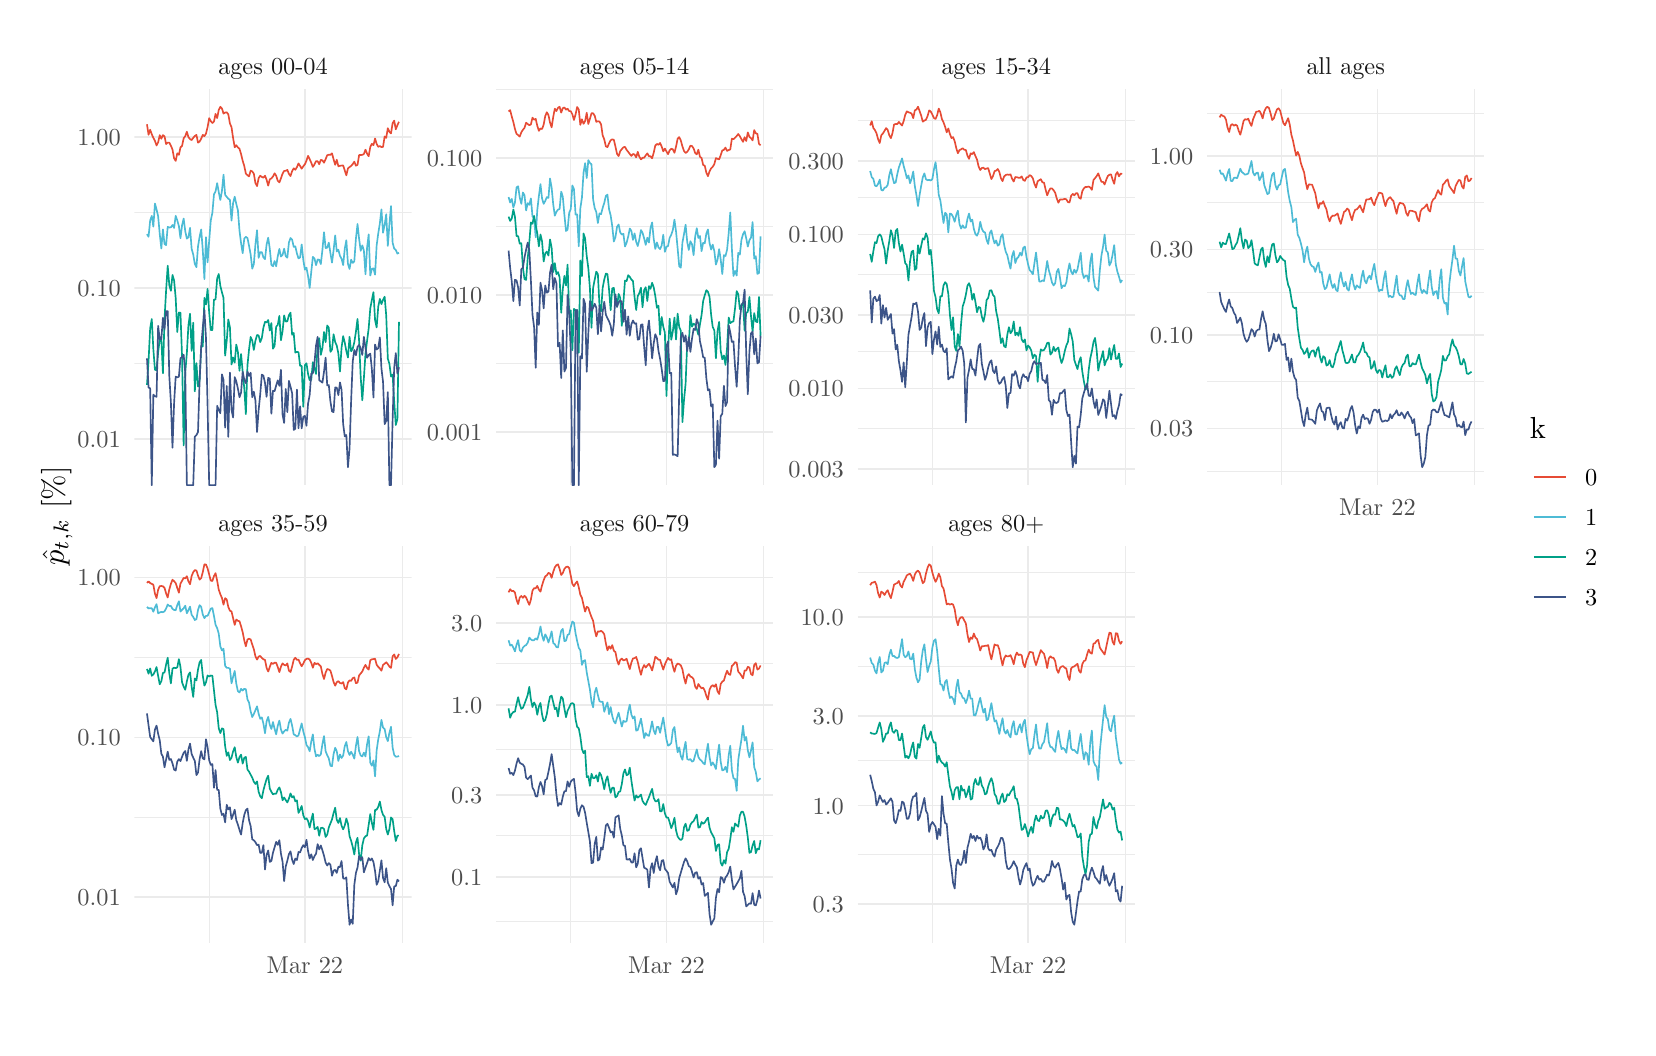
\begin{tikzpicture}[x=1pt,y=1pt]
\definecolor{fillColor}{RGB}{255,255,255}
\path[use as bounding box,fill=fillColor,fill opacity=0.00] (0,0) rectangle (578.16,361.35);
\begin{scope}
\path[clip] ( 38.56,196.02) rectangle (138.73,339.28);
\definecolor{drawColor}{gray}{0.92}

\path[draw=drawColor,line width= 0.3pt,line join=round] ( 38.56,240.06) --
	(138.73,240.06);

\path[draw=drawColor,line width= 0.3pt,line join=round] ( 38.56,294.53) --
	(138.73,294.53);

\path[draw=drawColor,line width= 0.3pt,line join=round] ( 65.59,196.02) --
	( 65.59,339.28);

\path[draw=drawColor,line width= 0.3pt,line join=round] (135.33,196.02) --
	(135.33,339.28);

\path[draw=drawColor,line width= 0.6pt,line join=round] ( 38.56,212.83) --
	(138.73,212.83);

\path[draw=drawColor,line width= 0.6pt,line join=round] ( 38.56,267.30) --
	(138.73,267.30);

\path[draw=drawColor,line width= 0.6pt,line join=round] ( 38.56,321.76) --
	(138.73,321.76);

\path[draw=drawColor,line width= 0.6pt,line join=round] (100.17,196.02) --
	(100.17,339.28);
\definecolor{drawColor}{RGB}{230,75,53}

\path[draw=drawColor,line width= 0.6pt,line join=round] ( 43.11,326.42) --
	( 43.68,322.65) --
	( 44.26,324.47) --
	( 44.84,322.84) --
	( 45.41,321.54) --
	( 45.99,320.46) --
	( 46.57,318.79) --
	( 47.14,319.90) --
	( 47.72,322.51) --
	( 48.30,321.21) --
	( 48.87,322.51) --
	( 49.45,322.07) --
	( 50.02,319.29) --
	( 50.60,319.82) --
	( 51.18,319.80) --
	( 51.75,318.72) --
	( 52.33,317.30) --
	( 52.91,314.14) --
	( 53.48,313.20) --
	( 54.06,315.96) --
	( 54.64,315.39) --
	( 55.21,318.07) --
	( 55.79,318.64) --
	( 56.36,321.36) --
	( 56.94,322.15) --
	( 57.52,323.77) --
	( 58.09,321.79) --
	( 58.67,321.09) --
	( 59.25,320.72) --
	( 59.82,321.54) --
	( 60.40,322.22) --
	( 60.98,322.59) --
	( 61.55,319.78) --
	( 62.13,320.20) --
	( 62.70,321.23) --
	( 63.28,322.62) --
	( 63.86,322.14) --
	( 64.43,323.04) --
	( 65.01,325.41) --
	( 65.59,328.64) --
	( 66.16,327.58) --
	( 66.74,326.91) --
	( 67.32,327.44) --
	( 67.89,330.19) --
	( 68.47,328.67) --
	( 69.04,331.60) --
	( 69.62,332.77) --
	( 70.20,332.11) --
	( 70.77,330.32) --
	( 71.35,330.67) --
	( 71.93,330.76) --
	( 72.50,330.04) --
	( 73.08,326.74) --
	( 73.66,325.38) --
	( 74.23,321.47) --
	( 74.81,318.13) --
	( 75.38,318.85) --
	( 75.96,318.07) --
	( 76.54,317.58) --
	( 77.11,315.67) --
	( 77.69,313.24) --
	( 78.27,311.35) --
	( 78.84,308.61) --
	( 79.42,308.04) --
	( 79.99,307.61) --
	( 80.57,309.68) --
	( 81.15,309.41) --
	( 81.72,308.58) --
	( 82.30,305.19) --
	( 82.88,304.10) --
	( 83.45,306.96) --
	( 84.03,307.85) --
	( 84.61,307.41) --
	( 85.18,307.15) --
	( 85.76,307.85) --
	( 86.33,306.41) --
	( 86.91,304.27) --
	( 87.49,306.55) --
	( 88.06,306.87) --
	( 88.64,307.58) --
	( 89.22,308.72) --
	( 89.79,307.84) --
	( 90.37,306.02) --
	( 90.95,305.43) --
	( 91.52,306.91) --
	( 92.10,308.57) --
	( 92.67,309.58) --
	( 93.25,309.62) --
	( 93.83,309.95) --
	( 94.40,308.53) --
	( 94.98,307.74) --
	( 95.56,309.51) --
	( 96.13,310.52) --
	( 96.71,309.99) --
	( 97.29,310.94) --
	( 97.86,312.29) --
	( 98.44,311.37) --
	( 99.01,310.38) --
	( 99.59,311.28) --
	(100.17,311.97) --
	(100.74,313.28) --
	(101.32,315.02) --
	(101.90,313.83) --
	(102.47,312.56) --
	(103.05,311.04) --
	(103.63,311.93) --
	(104.20,313.12) --
	(104.78,313.08) --
	(105.35,312.00) --
	(105.93,313.59) --
	(106.51,313.38) --
	(107.08,312.55) --
	(107.66,313.83) --
	(108.24,315.26) --
	(108.81,315.42) --
	(109.39,315.40) --
	(109.97,315.94) --
	(110.54,313.77) --
	(111.12,311.80) --
	(111.69,313.62) --
	(112.27,311.26) --
	(112.85,311.44) --
	(113.42,311.51) --
	(114.00,311.58) --
	(114.58,309.76) --
	(115.15,307.98) --
	(115.73,310.50) --
	(116.31,310.97) --
	(116.88,311.39) --
	(117.46,312.05) --
	(118.03,312.94) --
	(118.61,311.46) --
	(119.19,311.77) --
	(119.76,315.31) --
	(120.34,315.34) --
	(120.92,315.39) --
	(121.49,315.70) --
	(122.07,317.25) --
	(122.65,315.80) --
	(123.22,314.90) --
	(123.80,318.22) --
	(124.37,319.38) --
	(124.95,318.88) --
	(125.53,321.29) --
	(126.10,319.33) --
	(126.68,318.29) --
	(127.26,318.59) --
	(127.83,318.17) --
	(128.41,318.31) --
	(128.99,322.03) --
	(129.56,321.54) --
	(130.14,325.00) --
	(130.71,323.74) --
	(131.29,323.14) --
	(131.87,326.81) --
	(132.44,327.76) --
	(133.02,324.60) --
	(133.60,326.13) --
	(134.17,327.32);
\definecolor{drawColor}{RGB}{77,187,213}

\path[draw=drawColor,line width= 0.6pt,line join=round] ( 43.11,286.75) --
	( 43.68,285.80) --
	( 44.26,291.67) --
	( 44.84,293.33) --
	( 45.41,289.45) --
	( 45.99,297.81) --
	( 46.57,295.68) --
	( 47.14,293.19) --
	( 47.72,286.83) --
	( 48.30,281.54) --
	( 48.87,288.44) --
	( 49.45,283.15) --
	( 50.02,282.77) --
	( 50.60,289.38) --
	( 51.18,289.14) --
	( 51.75,289.20) --
	( 52.33,290.03) --
	( 52.91,288.98) --
	( 53.48,293.36) --
	( 54.06,291.70) --
	( 54.64,289.67) --
	( 55.21,285.28) --
	( 55.79,289.93) --
	( 56.36,292.37) --
	( 56.94,287.82) --
	( 57.52,285.09) --
	( 58.09,285.65) --
	( 58.67,288.99) --
	( 59.25,281.43) --
	( 59.82,279.39) --
	( 60.40,275.96) --
	( 60.98,274.81) --
	( 61.55,282.28) --
	( 62.13,285.82) --
	( 62.70,288.44) --
	( 63.28,280.86) --
	( 63.86,270.49) --
	( 64.43,285.66) --
	( 65.01,276.55) --
	( 65.59,284.37) --
	( 66.16,291.68) --
	( 66.74,294.45) --
	( 67.32,301.14) --
	( 67.89,302.17) --
	( 68.47,305.17) --
	( 69.04,301.97) --
	( 69.62,299.08) --
	( 70.20,302.38) --
	( 70.77,308.24) --
	( 71.35,300.94) --
	( 71.93,300.21) --
	( 72.50,299.53) --
	( 73.08,299.12) --
	( 73.66,291.62) --
	( 74.23,297.99) --
	( 74.81,300.27) --
	( 75.38,297.65) --
	( 75.96,295.41) --
	( 76.54,288.02) --
	( 77.11,283.49) --
	( 77.69,279.86) --
	( 78.27,285.14) --
	( 78.84,285.77) --
	( 79.42,285.34) --
	( 79.99,282.50) --
	( 80.57,279.40) --
	( 81.15,274.26) --
	( 81.72,275.88) --
	( 82.30,283.03) --
	( 82.88,288.14) --
	( 83.45,278.18) --
	( 84.03,280.23) --
	( 84.61,280.24) --
	( 85.18,278.32) --
	( 85.76,277.71) --
	( 86.33,282.96) --
	( 86.91,285.45) --
	( 87.49,281.39) --
	( 88.06,275.61) --
	( 88.64,275.14) --
	( 89.22,277.01) --
	( 89.79,275.13) --
	( 90.37,278.79) --
	( 90.95,281.38) --
	( 91.52,278.64) --
	( 92.10,279.20) --
	( 92.67,281.49) --
	( 93.25,278.78) --
	( 93.83,278.22) --
	( 94.40,283.70) --
	( 94.98,285.35) --
	( 95.56,284.73) --
	( 96.13,282.16) --
	( 96.71,282.32) --
	( 97.29,279.76) --
	( 97.86,277.96) --
	( 98.44,278.32) --
	( 99.01,283.01) --
	( 99.59,277.44) --
	(100.17,273.90) --
	(100.74,274.62) --
	(101.32,271.54) --
	(101.90,267.31) --
	(102.47,273.07) --
	(103.05,278.52) --
	(103.63,277.97) --
	(104.20,275.54) --
	(104.78,277.59) --
	(105.35,277.49) --
	(105.93,275.92) --
	(106.51,281.06) --
	(107.08,287.44) --
	(107.66,281.72) --
	(108.24,281.83) --
	(108.81,283.66) --
	(109.39,279.93) --
	(109.97,276.45) --
	(110.54,280.91) --
	(111.12,286.29) --
	(111.69,280.46) --
	(112.27,281.10) --
	(112.85,278.88) --
	(113.42,277.86) --
	(114.00,275.54) --
	(114.58,281.47) --
	(115.15,284.54) --
	(115.73,276.00) --
	(116.31,274.15) --
	(116.88,277.51) --
	(117.46,276.34) --
	(118.03,276.94) --
	(118.61,285.10) --
	(119.19,290.39) --
	(119.76,285.06) --
	(120.34,280.72) --
	(120.92,282.69) --
	(121.49,280.79) --
	(122.07,272.24) --
	(122.65,281.94) --
	(123.22,286.65) --
	(123.80,271.78) --
	(124.37,274.19) --
	(124.95,274.40) --
	(125.53,272.10) --
	(126.10,282.65) --
	(126.68,287.02) --
	(127.26,290.62) --
	(127.83,295.68) --
	(128.41,287.25) --
	(128.99,290.10) --
	(129.56,293.93) --
	(130.14,282.47) --
	(130.71,290.26) --
	(131.29,296.87) --
	(131.87,283.65) --
	(132.44,281.52) --
	(133.02,281.03) --
	(133.60,279.70) --
	(134.17,280.01);
\definecolor{drawColor}{RGB}{0,160,135}

\path[draw=drawColor,line width= 0.6pt,line join=round] ( 43.11,232.28) --
	( 43.68,240.92) --
	( 44.26,252.68) --
	( 44.84,256.06) --
	( 45.41,245.17) --
	( 45.99,237.75) --
	( 46.57,237.56) --
	( 47.14,244.00) --
	( 47.72,248.76) --
	( 48.30,248.74) --
	( 48.87,236.46) --
	( 49.45,256.06) --
	( 50.02,266.38) --
	( 50.60,275.32) --
	( 51.18,268.27) --
	( 51.75,266.27) --
	( 52.33,272.00) --
	( 52.91,270.00) --
	( 53.48,263.72) --
	( 54.06,251.38) --
	( 54.64,258.40) --
	( 55.21,258.33) --
	( 55.79,242.27) --
	( 56.36,210.39) --
	( 56.94,236.74) --
	( 57.52,243.72) --
	( 58.09,253.86) --
	( 58.67,257.96) --
	( 59.25,244.58) --
	( 59.82,254.76) --
	( 60.40,229.93) --
	( 60.98,240.13) --
	( 61.55,231.66) --
	( 62.13,233.84) --
	( 62.70,246.06) --
	( 63.28,246.17) --
	( 63.86,263.69) --
	( 64.43,261.30) --
	( 65.01,266.96) --
	( 65.59,258.38) --
	( 66.16,252.08) --
	( 66.74,252.07) --
	( 67.32,263.07) --
	( 67.89,263.17) --
	( 68.47,270.75) --
	( 69.04,272.33) --
	( 69.62,268.04) --
	( 70.20,265.70) --
	( 70.77,263.70) --
	( 71.35,242.83) --
	( 71.93,248.24) --
	( 72.50,255.87) --
	( 73.08,253.09) --
	( 73.66,239.65) --
	( 74.23,242.15) --
	( 74.81,240.34) --
	( 75.38,246.83) --
	( 75.96,244.20) --
	( 76.54,237.40) --
	( 77.11,243.41) --
	( 77.69,236.99) --
	( 78.27,231.02) --
	( 78.84,221.72) --
	( 79.42,239.31) --
	( 79.99,245.07) --
	( 80.57,249.59) --
	( 81.15,248.27) --
	( 81.72,244.90) --
	( 82.30,248.26) --
	( 82.88,250.29) --
	( 83.45,250.14) --
	( 84.03,247.73) --
	( 84.61,249.20) --
	( 85.18,252.97) --
	( 85.76,255.05) --
	( 86.33,254.82) --
	( 86.91,255.70) --
	( 87.49,251.89) --
	( 88.06,254.62) --
	( 88.64,245.33) --
	( 89.22,246.38) --
	( 89.79,253.28) --
	( 90.37,253.96) --
	( 90.95,257.19) --
	( 91.52,248.40) --
	( 92.10,251.68) --
	( 92.67,257.36) --
	( 93.25,255.16) --
	( 93.83,255.23) --
	( 94.40,257.45) --
	( 94.98,258.37) --
	( 95.56,250.38) --
	( 96.13,251.04) --
	( 96.71,243.95) --
	( 97.29,244.18) --
	( 97.86,244.08) --
	( 98.44,239.18) --
	( 99.01,239.15) --
	( 99.59,224.36) --
	(100.17,239.36) --
	(100.74,240.08) --
	(101.32,236.20) --
	(101.90,233.94) --
	(102.47,234.08) --
	(103.05,240.45) --
	(103.63,238.37) --
	(104.20,236.22) --
	(104.78,246.98) --
	(105.35,249.14) --
	(105.93,243.12) --
	(106.51,245.64) --
	(107.08,251.39) --
	(107.66,247.71) --
	(108.24,253.73) --
	(108.81,252.92) --
	(109.39,244.19) --
	(109.97,245.01) --
	(110.54,250.55) --
	(111.12,247.75) --
	(111.69,246.45) --
	(112.27,243.59) --
	(112.85,237.11) --
	(113.42,245.69) --
	(114.00,249.90) --
	(114.58,247.58) --
	(115.15,244.46) --
	(115.73,242.13) --
	(116.31,249.64) --
	(116.88,244.37) --
	(117.46,245.36) --
	(118.03,247.69) --
	(118.61,251.44) --
	(119.19,256.10) --
	(119.76,248.20) --
	(120.34,235.07) --
	(120.92,226.70) --
	(121.49,234.76) --
	(122.07,243.55) --
	(122.65,248.25) --
	(123.22,252.70) --
	(123.80,259.94) --
	(124.37,262.95) --
	(124.95,265.78) --
	(125.53,255.71) --
	(126.10,253.02) --
	(126.68,260.58) --
	(127.26,263.35) --
	(127.83,261.45) --
	(128.41,263.02) --
	(128.99,264.11) --
	(129.56,257.33) --
	(130.14,241.72) --
	(130.71,239.92) --
	(131.29,235.30) --
	(131.87,235.99) --
	(132.44,226.28) --
	(133.02,217.77) --
	(133.60,219.96) --
	(134.17,255.03);
\definecolor{drawColor}{RGB}{60,84,136}

\path[draw=drawColor,line width= 0.6pt,line join=round] ( 43.11,241.87) --
	( 43.68,231.33) --
	( 44.26,231.00) --
	( 44.84,196.02) --
	( 45.41,228.77) --
	( 45.99,228.16) --
	( 46.57,227.97) --
	( 47.14,253.59) --
	( 47.72,248.76) --
	( 48.30,248.74) --
	( 48.87,256.51) --
	( 49.45,252.42) --
	( 50.02,258.84) --
	( 50.60,258.92) --
	( 51.18,235.47) --
	( 51.75,225.94) --
	( 52.33,209.58) --
	( 52.91,225.73) --
	( 53.48,235.24) --
	( 54.06,234.98) --
	( 54.64,235.20) --
	( 55.21,241.93) --
	( 55.79,242.27) --
	( 56.36,243.18) --
	( 56.94,236.74) --
	( 57.52,196.02) --
	( 58.09,196.02) --
	( 58.67,196.02) --
	( 59.25,196.02) --
	( 59.82,196.02) --
	( 60.40,213.53) --
	( 60.98,214.14) --
	( 61.55,215.26) --
	( 62.13,233.84) --
	( 62.70,246.06) --
	( 63.28,252.98) --
	( 63.86,259.38) --
	( 64.43,249.22) --
	( 65.01,224.58) --
	( 65.59,196.02) --
	( 66.16,196.02) --
	( 66.74,196.02) --
	( 67.32,196.02) --
	( 67.89,196.02) --
	( 68.47,224.72) --
	( 69.04,223.15) --
	( 69.62,222.02) --
	( 70.20,236.07) --
	( 70.77,234.07) --
	( 71.35,216.84) --
	( 71.93,231.84) --
	( 72.50,213.49) --
	( 73.08,236.69) --
	( 73.66,223.25) --
	( 74.23,220.48) --
	( 74.81,235.06) --
	( 75.38,233.59) --
	( 75.96,230.96) --
	( 76.54,227.81) --
	( 77.11,229.50) --
	( 77.69,236.99) --
	( 78.27,234.17) --
	( 78.84,232.83) --
	( 79.42,237.06) --
	( 79.99,235.48) --
	( 80.57,236.67) --
	( 81.15,227.81) --
	( 81.72,229.85) --
	( 82.30,226.58) --
	( 82.88,215.24) --
	( 83.45,223.05) --
	( 84.03,228.85) --
	( 84.61,235.97) --
	( 85.18,235.61) --
	( 85.76,232.95) --
	( 86.33,227.97) --
	( 86.91,234.83) --
	( 87.49,234.53) --
	( 88.06,221.83) --
	( 88.64,230.15) --
	( 89.22,229.99) --
	( 89.79,232.04) --
	( 90.37,233.91) --
	( 90.95,231.93) --
	( 91.52,237.71) --
	( 92.10,221.57) --
	( 92.67,218.51) --
	( 93.25,230.80) --
	( 93.83,222.44) --
	( 94.40,233.72) --
	( 94.98,231.60) --
	( 95.56,229.24) --
	( 96.13,215.99) --
	( 96.71,216.44) --
	( 97.29,230.57) --
	( 97.86,216.57) --
	( 98.44,224.54) --
	( 99.01,216.55) --
	( 99.59,220.72) --
	(100.17,221.07) --
	(100.74,217.48) --
	(101.32,225.51) --
	(101.90,228.66) --
	(102.47,236.33) --
	(103.05,236.50) --
	(103.63,240.26) --
	(104.20,246.51) --
	(104.78,249.61) --
	(105.35,233.96) --
	(105.93,233.53) --
	(106.51,233.09) --
	(107.08,237.05) --
	(107.66,242.12) --
	(108.24,232.06) --
	(108.81,232.21) --
	(109.39,226.36) --
	(109.97,222.67) --
	(110.54,222.41) --
	(111.12,231.35) --
	(111.69,231.27) --
	(112.27,228.55) --
	(112.85,233.16) --
	(113.42,230.51) --
	(114.00,218.11) --
	(114.58,213.63) --
	(115.15,214.16) --
	(115.73,202.53) --
	(116.31,209.32) --
	(116.88,226.54) --
	(117.46,240.77) --
	(118.03,244.90) --
	(118.61,243.00) --
	(119.19,245.99) --
	(119.76,246.68) --
	(120.34,245.52) --
	(120.92,243.09) --
	(121.49,249.63) --
	(122.07,245.61) --
	(122.65,242.05) --
	(123.22,243.11) --
	(123.80,243.54) --
	(124.37,237.97) --
	(124.95,227.71) --
	(125.53,246.84) --
	(126.10,245.06) --
	(126.68,245.53) --
	(127.26,249.45) --
	(127.83,238.25) --
	(128.41,233.38) --
	(128.99,218.08) --
	(129.56,219.26) --
	(130.14,229.64) --
	(130.71,196.02) --
	(131.29,196.02) --
	(131.87,219.59) --
	(132.44,238.36) --
	(133.02,243.76) --
	(133.60,236.35) --
	(134.17,238.63);
\end{scope}
\begin{scope}
\path[clip] ( 38.56, 30.69) rectangle (138.73,173.95);
\definecolor{drawColor}{gray}{0.92}

\path[draw=drawColor,line width= 0.3pt,line join=round] ( 38.56, 76.00) --
	(138.73, 76.00);

\path[draw=drawColor,line width= 0.3pt,line join=round] ( 38.56,133.76) --
	(138.73,133.76);

\path[draw=drawColor,line width= 0.3pt,line join=round] ( 65.59, 30.69) --
	( 65.59,173.95);

\path[draw=drawColor,line width= 0.3pt,line join=round] (135.33, 30.69) --
	(135.33,173.95);

\path[draw=drawColor,line width= 0.6pt,line join=round] ( 38.56, 47.12) --
	(138.73, 47.12);

\path[draw=drawColor,line width= 0.6pt,line join=round] ( 38.56,104.88) --
	(138.73,104.88);

\path[draw=drawColor,line width= 0.6pt,line join=round] ( 38.56,162.64) --
	(138.73,162.64);

\path[draw=drawColor,line width= 0.6pt,line join=round] (100.17, 30.69) --
	(100.17,173.95);
\definecolor{drawColor}{RGB}{230,75,53}

\path[draw=drawColor,line width= 0.6pt,line join=round] ( 43.11,160.74) --
	( 43.68,161.27) --
	( 44.26,160.66) --
	( 44.84,160.38) --
	( 45.41,160.06) --
	( 45.99,156.84) --
	( 46.57,155.23) --
	( 47.14,158.24) --
	( 47.72,159.52) --
	( 48.30,159.60) --
	( 48.87,159.48) --
	( 49.45,158.93) --
	( 50.02,156.93) --
	( 50.60,155.45) --
	( 51.18,158.37) --
	( 51.75,160.36) --
	( 52.33,161.86) --
	( 52.91,161.33) --
	( 53.48,160.64) --
	( 54.06,158.88) --
	( 54.64,157.17) --
	( 55.21,160.48) --
	( 55.79,161.47) --
	( 56.36,162.53) --
	( 56.94,162.33) --
	( 57.52,163.13) --
	( 58.09,161.30) --
	( 58.67,160.23) --
	( 59.25,163.22) --
	( 59.82,164.60) --
	( 60.40,165.33) --
	( 60.98,165.22) --
	( 61.55,163.36) --
	( 62.13,161.88) --
	( 62.70,162.44) --
	( 63.28,164.63) --
	( 63.86,167.43) --
	( 64.43,167.35) --
	( 65.01,165.96) --
	( 65.59,163.73) --
	( 66.16,161.56) --
	( 66.74,161.40) --
	( 67.32,163.18) --
	( 67.89,164.22) --
	( 68.47,161.51) --
	( 69.04,158.28) --
	( 69.62,156.61) --
	( 70.20,155.29) --
	( 70.77,152.86) --
	( 71.35,155.20) --
	( 71.93,154.71) --
	( 72.50,152.02) --
	( 73.08,150.66) --
	( 73.66,150.42) --
	( 74.23,147.96) --
	( 74.81,145.55) --
	( 75.38,147.49) --
	( 75.96,147.02) --
	( 76.54,146.85) --
	( 77.11,145.06) --
	( 77.69,142.90) --
	( 78.27,139.92) --
	( 78.84,137.82) --
	( 79.42,140.27) --
	( 79.99,140.54) --
	( 80.57,140.28) --
	( 81.15,138.45) --
	( 81.72,136.78) --
	( 82.30,134.20) --
	( 82.88,133.01) --
	( 83.45,134.10) --
	( 84.03,134.32) --
	( 84.61,133.61) --
	( 85.18,133.11) --
	( 85.76,132.89) --
	( 86.33,129.99) --
	( 86.91,128.68) --
	( 87.49,130.42) --
	( 88.06,131.80) --
	( 88.64,131.47) --
	( 89.22,131.89) --
	( 89.79,131.85) --
	( 90.37,130.30) --
	( 90.95,128.48) --
	( 91.52,130.43) --
	( 92.10,131.65) --
	( 92.67,131.12) --
	( 93.25,130.87) --
	( 93.83,131.63) --
	( 94.40,129.01) --
	( 94.98,128.52) --
	( 95.56,130.49) --
	( 96.13,132.93) --
	( 96.71,133.67) --
	( 97.29,132.93) --
	( 97.86,133.01) --
	( 98.44,131.66) --
	( 99.01,130.60) --
	( 99.59,131.56) --
	(100.17,132.77) --
	(100.74,133.25) --
	(101.32,133.38) --
	(101.90,133.02) --
	(102.47,131.89) --
	(103.05,130.07) --
	(103.63,131.82) --
	(104.20,131.37) --
	(104.78,131.68) --
	(105.35,131.10) --
	(105.93,130.55) --
	(106.51,127.78) --
	(107.08,125.99) --
	(107.66,128.27) --
	(108.24,129.61) --
	(108.81,129.43) --
	(109.39,129.03) --
	(109.97,127.08) --
	(110.54,124.91) --
	(111.12,123.57) --
	(111.69,124.85) --
	(112.27,125.22) --
	(112.85,124.54) --
	(113.42,124.35) --
	(114.00,124.87) --
	(114.58,122.68) --
	(115.15,122.25) --
	(115.73,124.71) --
	(116.31,125.52) --
	(116.88,125.31) --
	(117.46,126.31) --
	(118.03,126.54) --
	(118.61,124.47) --
	(119.19,124.68) --
	(119.76,127.30) --
	(120.34,127.98) --
	(120.92,128.72) --
	(121.49,130.06) --
	(122.07,131.08) --
	(122.65,129.99) --
	(123.22,129.38) --
	(123.80,132.78) --
	(124.37,133.10) --
	(124.95,133.19) --
	(125.53,133.31) --
	(126.10,131.15) --
	(126.68,130.37) --
	(127.26,129.79) --
	(127.83,128.99) --
	(128.41,131.08) --
	(128.99,131.51) --
	(129.56,132.04) --
	(130.14,131.37) --
	(130.71,130.46) --
	(131.29,130.00) --
	(131.87,134.19) --
	(132.44,134.86) --
	(133.02,133.22) --
	(133.60,133.85) --
	(134.17,135.05);
\definecolor{drawColor}{RGB}{77,187,213}

\path[draw=drawColor,line width= 0.6pt,line join=round] ( 43.11,152.06) --
	( 43.68,151.49) --
	( 44.26,151.57) --
	( 44.84,151.58) --
	( 45.41,150.30) --
	( 45.99,151.91) --
	( 46.57,153.03) --
	( 47.14,149.72) --
	( 47.72,150.03) --
	( 48.30,150.26) --
	( 48.87,150.12) --
	( 49.45,150.44) --
	( 50.02,151.47) --
	( 50.60,152.90) --
	( 51.18,152.39) --
	( 51.75,152.40) --
	( 52.33,151.34) --
	( 52.91,150.95) --
	( 53.48,150.84) --
	( 54.06,152.72) --
	( 54.64,154.07) --
	( 55.21,150.36) --
	( 55.79,151.00) --
	( 56.36,151.54) --
	( 56.94,152.47) --
	( 57.52,149.74) --
	( 58.09,150.90) --
	( 58.67,152.12) --
	( 59.25,149.15) --
	( 59.82,148.43) --
	( 60.40,147.30) --
	( 60.98,147.61) --
	( 61.55,150.93) --
	( 62.13,152.66) --
	( 62.70,152.05) --
	( 63.28,149.26) --
	( 63.86,147.99) --
	( 64.43,148.80) --
	( 65.01,148.82) --
	( 65.59,150.09) --
	( 66.16,151.41) --
	( 66.74,151.63) --
	( 67.32,148.73) --
	( 67.89,145.59) --
	( 68.47,144.40) --
	( 69.04,142.36) --
	( 69.62,137.78) --
	( 70.20,136.32) --
	( 70.77,136.92) --
	( 71.35,130.77) --
	( 71.93,130.03) --
	( 72.50,130.02) --
	( 73.08,129.73) --
	( 73.66,124.44) --
	( 74.23,126.78) --
	( 74.81,128.92) --
	( 75.38,124.31) --
	( 75.96,121.59) --
	( 76.54,121.12) --
	( 77.11,122.44) --
	( 77.69,121.82) --
	( 78.27,122.44) --
	( 78.84,122.29) --
	( 79.42,118.64) --
	( 79.99,117.43) --
	( 80.57,114.31) --
	( 81.15,112.23) --
	( 81.72,113.33) --
	( 82.30,114.73) --
	( 82.88,116.12) --
	( 83.45,113.45) --
	( 84.03,111.62) --
	( 84.61,112.11) --
	( 85.18,109.87) --
	( 85.76,106.40) --
	( 86.33,110.68) --
	( 86.91,112.30) --
	( 87.49,109.42) --
	( 88.06,107.94) --
	( 88.64,110.45) --
	( 89.22,107.99) --
	( 89.79,105.99) --
	( 90.37,109.12) --
	( 90.95,110.96) --
	( 91.52,107.74) --
	( 92.10,106.27) --
	( 92.67,107.08) --
	( 93.25,107.62) --
	( 93.83,107.30) --
	( 94.40,110.22) --
	( 94.98,111.56) --
	( 95.56,109.13) --
	( 96.13,105.97) --
	( 96.71,105.70) --
	( 97.29,105.20) --
	( 97.86,105.62) --
	( 98.44,107.80) --
	( 99.01,109.94) --
	( 99.59,107.06) --
	(100.17,104.98) --
	(100.74,102.18) --
	(101.32,101.35) --
	(101.90, 99.89) --
	(102.47,103.37) --
	(103.05,105.99) --
	(103.63,100.77) --
	(104.20, 98.03) --
	(104.78, 98.61) --
	(105.35, 98.12) --
	(105.93, 98.76) --
	(106.51,102.54) --
	(107.08,105.35) --
	(107.66, 99.88) --
	(108.24, 98.45) --
	(108.81, 97.30) --
	(109.39, 94.65) --
	(109.97, 94.48) --
	(110.54, 98.89) --
	(111.12,101.15) --
	(111.69, 99.89) --
	(112.27, 96.37) --
	(112.85, 98.71) --
	(113.42, 97.47) --
	(114.00, 98.34) --
	(114.58,101.73) --
	(115.15,103.23) --
	(115.73, 99.93) --
	(116.31, 98.53) --
	(116.88, 99.69) --
	(117.46, 98.63) --
	(118.03, 97.22) --
	(118.61,101.81) --
	(119.19,105.05) --
	(119.76, 99.90) --
	(120.34, 98.34) --
	(120.92, 98.02) --
	(121.49, 99.38) --
	(122.07, 98.00) --
	(122.65,102.51) --
	(123.22,105.27) --
	(123.80, 95.74) --
	(124.37, 94.66) --
	(124.95, 96.56) --
	(125.53, 90.81) --
	(126.10,100.18) --
	(126.68,104.23) --
	(127.26,107.09) --
	(127.83,111.20) --
	(128.41,108.43) --
	(128.99,107.92) --
	(129.56,104.96) --
	(130.14,103.53) --
	(130.71,106.55) --
	(131.29,108.71) --
	(131.87,101.23) --
	(132.44, 98.55) --
	(133.02, 97.92) --
	(133.60, 97.94) --
	(134.17, 98.18);
\definecolor{drawColor}{RGB}{0,160,135}

\path[draw=drawColor,line width= 0.6pt,line join=round] ( 43.11,129.61) --
	( 43.68,127.90) --
	( 44.26,129.83) --
	( 44.84,127.16) --
	( 45.41,127.63) --
	( 45.99,128.71) --
	( 46.57,130.32) --
	( 47.14,127.09) --
	( 47.72,124.08) --
	( 48.30,125.19) --
	( 48.87,128.18) --
	( 49.45,128.35) --
	( 50.02,131.24) --
	( 50.60,133.65) --
	( 51.18,128.06) --
	( 51.75,124.38) --
	( 52.33,129.72) --
	( 52.91,130.08) --
	( 53.48,129.90) --
	( 54.06,130.19) --
	( 54.64,133.15) --
	( 55.21,130.34) --
	( 55.79,124.77) --
	( 56.36,123.27) --
	( 56.94,122.10) --
	( 57.52,125.12) --
	( 58.09,127.52) --
	( 58.67,128.39) --
	( 59.25,123.18) --
	( 59.82,119.52) --
	( 60.40,126.19) --
	( 60.98,125.49) --
	( 61.55,129.42) --
	( 62.13,132.07) --
	( 62.70,132.88) --
	( 63.28,127.18) --
	( 63.86,123.58) --
	( 64.43,124.79) --
	( 65.01,127.26) --
	( 65.59,126.88) --
	( 66.16,127.25) --
	( 66.74,127.16) --
	( 67.32,121.84) --
	( 67.89,116.61) --
	( 68.47,113.97) --
	( 69.04,108.25) --
	( 69.62,106.43) --
	( 70.20,108.15) --
	( 70.77,107.88) --
	( 71.35,101.72) --
	( 71.93, 98.22) --
	( 72.50, 99.51) --
	( 73.08, 96.71) --
	( 73.66, 97.58) --
	( 74.23, 99.82) --
	( 74.81,101.36) --
	( 75.38, 97.77) --
	( 75.96, 95.76) --
	( 76.54, 97.80) --
	( 77.11, 98.65) --
	( 77.69, 95.42) --
	( 78.27, 97.52) --
	( 78.84, 97.84) --
	( 79.42, 93.26) --
	( 79.99, 92.53) --
	( 80.57, 91.42) --
	( 81.15, 90.35) --
	( 81.72, 88.86) --
	( 82.30, 88.07) --
	( 82.88, 89.00) --
	( 83.45, 85.24) --
	( 84.03, 83.61) --
	( 84.61, 82.90) --
	( 85.18, 85.75) --
	( 85.76, 87.92) --
	( 86.33, 89.84) --
	( 86.91, 91.06) --
	( 87.49, 86.36) --
	( 88.06, 85.24) --
	( 88.64, 84.29) --
	( 89.22, 84.57) --
	( 89.79, 84.54) --
	( 90.37, 85.99) --
	( 90.95, 86.82) --
	( 91.52, 85.13) --
	( 92.10, 82.16) --
	( 92.67, 83.17) --
	( 93.25, 82.23) --
	( 93.83, 81.39) --
	( 94.40, 82.76) --
	( 94.98, 84.65) --
	( 95.56, 83.22) --
	( 96.13, 83.64) --
	( 96.71, 81.79) --
	( 97.29, 82.15) --
	( 97.86, 77.61) --
	( 98.44, 78.74) --
	( 99.01, 80.12) --
	( 99.59, 76.74) --
	(100.17, 75.38) --
	(100.74, 75.69) --
	(101.32, 74.66) --
	(101.90, 72.32) --
	(102.47, 75.01) --
	(103.05, 77.38) --
	(103.63, 71.77) --
	(104.20, 71.95) --
	(104.78, 72.55) --
	(105.35, 69.35) --
	(105.93, 72.15) --
	(106.51, 72.25) --
	(107.08, 71.78) --
	(107.66, 68.92) --
	(108.24, 69.77) --
	(108.81, 72.34) --
	(109.39, 73.80) --
	(109.97, 75.27) --
	(110.54, 77.56) --
	(111.12, 79.49) --
	(111.69, 75.07) --
	(112.27, 73.97) --
	(112.85, 75.73) --
	(113.42, 72.99) --
	(114.00, 71.65) --
	(114.58, 73.07) --
	(115.15, 75.57) --
	(115.73, 73.71) --
	(116.31, 69.22) --
	(116.88, 67.54) --
	(117.46, 65.31) --
	(118.03, 62.57) --
	(118.61, 66.92) --
	(119.19, 68.61) --
	(119.76, 62.64) --
	(120.34, 60.35) --
	(120.92, 65.92) --
	(121.49, 68.38) --
	(122.07, 69.18) --
	(122.65, 69.41) --
	(123.22, 73.28) --
	(123.80, 77.18) --
	(124.37, 74.04) --
	(124.95, 71.47) --
	(125.53, 78.70) --
	(126.10, 78.77) --
	(126.68, 79.81) --
	(127.26, 81.71) --
	(127.83, 78.68) --
	(128.41, 76.91) --
	(128.99, 76.20) --
	(129.56, 71.78) --
	(130.14, 69.78) --
	(130.71, 71.77) --
	(131.29, 75.96) --
	(131.87, 75.33) --
	(132.44, 71.10) --
	(133.02, 67.42) --
	(133.60, 69.39) --
	(134.17, 69.39);
\definecolor{drawColor}{RGB}{60,84,136}

\path[draw=drawColor,line width= 0.6pt,line join=round] ( 43.11,113.54) --
	( 43.68,109.24) --
	( 44.26,105.05) --
	( 44.84,104.21) --
	( 45.41,103.45) --
	( 45.99,107.74) --
	( 46.57,109.15) --
	( 47.14,106.21) --
	( 47.72,103.86) --
	( 48.30, 98.98) --
	( 48.87, 97.93) --
	( 49.45, 94.07) --
	( 50.02, 96.91) --
	( 50.60, 99.73) --
	( 51.18, 96.74) --
	( 51.75, 97.08) --
	( 52.33, 95.50) --
	( 52.91, 93.25) --
	( 53.48, 92.92) --
	( 54.06, 96.14) --
	( 54.64, 97.04) --
	( 55.21, 96.32) --
	( 55.79, 97.90) --
	( 56.36, 99.30) --
	( 56.94, 99.97) --
	( 57.52, 96.41) --
	( 58.09,100.59) --
	( 58.67,102.64) --
	( 59.25, 98.88) --
	( 59.82, 97.59) --
	( 60.40, 96.40) --
	( 60.98, 91.25) --
	( 61.55, 92.22) --
	( 62.13, 97.06) --
	( 62.70, 99.94) --
	( 63.28, 97.29) --
	( 63.86, 96.94) --
	( 64.43,104.21) --
	( 65.01,101.30) --
	( 65.59, 96.62) --
	( 66.16, 94.96) --
	( 66.74, 95.27) --
	( 67.32, 86.70) --
	( 67.89, 93.08) --
	( 68.47, 85.95) --
	( 69.04, 85.92) --
	( 69.62, 79.14) --
	( 70.20, 76.84) --
	( 70.77, 77.31) --
	( 71.35, 74.16) --
	( 71.93, 80.53) --
	( 72.50, 78.89) --
	( 73.08, 79.62) --
	( 73.66, 75.36) --
	( 74.23, 76.95) --
	( 74.81, 78.78) --
	( 75.38, 75.01) --
	( 75.96, 73.37) --
	( 76.54, 71.47) --
	( 77.11, 69.77) --
	( 77.69, 73.91) --
	( 78.27, 76.90) --
	( 78.84, 78.57) --
	( 79.42, 79.14) --
	( 79.99, 74.98) --
	( 80.57, 72.84) --
	( 81.15, 68.07) --
	( 81.72, 67.71) --
	( 82.30, 67.02) --
	( 82.88, 65.94) --
	( 83.45, 66.15) --
	( 84.03, 63.14) --
	( 84.61, 63.18) --
	( 85.18, 65.94) --
	( 85.76, 57.17) --
	( 86.33, 62.39) --
	( 86.91, 64.03) --
	( 87.49, 59.90) --
	( 88.06, 60.24) --
	( 88.64, 63.21) --
	( 89.22, 65.17) --
	( 89.79, 67.15) --
	( 90.37, 66.06) --
	( 90.95, 67.74) --
	( 91.52, 62.89) --
	( 92.10, 60.02) --
	( 92.67, 52.92) --
	( 93.25, 58.26) --
	( 93.83, 60.34) --
	( 94.40, 62.71) --
	( 94.98, 63.71) --
	( 95.56, 60.67) --
	( 96.13, 59.13) --
	( 96.71, 61.12) --
	( 97.29, 60.57) --
	( 97.86, 63.48) --
	( 98.44, 63.31) --
	( 99.01, 64.94) --
	( 99.59, 65.94) --
	(100.17, 65.21) --
	(100.74, 67.87) --
	(101.32, 63.78) --
	(101.90, 61.13) --
	(102.47, 62.64) --
	(103.05, 60.59) --
	(103.63, 61.97) --
	(104.20, 62.83) --
	(104.78, 66.31) --
	(105.35, 64.42) --
	(105.93, 65.85) --
	(106.51, 64.06) --
	(107.08, 62.12) --
	(107.66, 59.64) --
	(108.24, 58.61) --
	(108.81, 59.46) --
	(109.39, 58.88) --
	(109.97, 54.89) --
	(110.54, 56.72) --
	(111.12, 57.02) --
	(111.69, 55.91) --
	(112.27, 58.14) --
	(112.85, 58.04) --
	(113.42, 60.23) --
	(114.00, 53.92) --
	(114.58, 53.83) --
	(115.15, 54.32) --
	(115.73, 44.47) --
	(116.31, 37.20) --
	(116.88, 39.12) --
	(117.46, 37.52) --
	(118.03, 51.58) --
	(118.61, 55.91) --
	(119.19, 57.85) --
	(119.76, 62.03) --
	(120.34, 60.69) --
	(120.92, 61.63) --
	(121.49, 56.10) --
	(122.07, 57.88) --
	(122.65, 59.51) --
	(123.22, 61.29) --
	(123.80, 60.44) --
	(124.37, 61.15) --
	(124.95, 59.85) --
	(125.53, 56.56) --
	(126.10, 51.64) --
	(126.68, 52.95) --
	(127.26, 56.79) --
	(127.83, 60.47) --
	(128.41, 54.09) --
	(128.99, 52.50) --
	(129.56, 57.64) --
	(130.14, 52.39) --
	(130.71, 51.18) --
	(131.29, 50.08) --
	(131.87, 44.21) --
	(132.44, 51.06) --
	(133.02, 51.13) --
	(133.60, 53.48) --
	(134.17, 52.83);
\end{scope}
\begin{scope}
\path[clip] (169.22,196.02) rectangle (269.39,339.28);
\definecolor{drawColor}{gray}{0.92}

\path[draw=drawColor,line width= 0.3pt,line join=round] (169.22,239.98) --
	(269.39,239.98);

\path[draw=drawColor,line width= 0.3pt,line join=round] (169.22,289.43) --
	(269.39,289.43);

\path[draw=drawColor,line width= 0.3pt,line join=round] (169.22,338.88) --
	(269.39,338.88);

\path[draw=drawColor,line width= 0.3pt,line join=round] (196.25,196.02) --
	(196.25,339.28);

\path[draw=drawColor,line width= 0.3pt,line join=round] (265.99,196.02) --
	(265.99,339.28);

\path[draw=drawColor,line width= 0.6pt,line join=round] (169.22,215.26) --
	(269.39,215.26);

\path[draw=drawColor,line width= 0.6pt,line join=round] (169.22,264.71) --
	(269.39,264.71);

\path[draw=drawColor,line width= 0.6pt,line join=round] (169.22,314.15) --
	(269.39,314.15);

\path[draw=drawColor,line width= 0.6pt,line join=round] (230.83,196.02) --
	(230.83,339.28);
\definecolor{drawColor}{RGB}{230,75,53}

\path[draw=drawColor,line width= 0.6pt,line join=round] (173.77,331.06) --
	(174.34,331.55) --
	(174.92,329.23) --
	(175.50,327.25) --
	(176.07,324.76) --
	(176.65,323.00) --
	(177.23,322.52) --
	(177.80,322.00) --
	(178.38,323.55) --
	(178.96,324.44) --
	(179.53,325.16) --
	(180.11,327.01) --
	(180.68,326.54) --
	(181.26,326.08) --
	(181.84,326.40) --
	(182.41,328.81) --
	(182.99,328.09) --
	(183.57,328.40) --
	(184.14,325.92) --
	(184.72,324.08) --
	(185.30,324.90) --
	(185.87,324.72) --
	(186.45,326.30) --
	(187.02,329.40) --
	(187.60,330.79) --
	(188.18,329.77) --
	(188.75,327.04) --
	(189.33,325.34) --
	(189.91,329.11) --
	(190.48,332.08) --
	(191.06,331.22) --
	(191.64,332.39) --
	(192.21,332.77) --
	(192.79,330.65) --
	(193.36,332.24) --
	(193.94,332.51) --
	(194.52,331.70) --
	(195.09,332.08) --
	(195.67,331.22) --
	(196.25,331.16) --
	(196.82,330.03) --
	(197.40,327.98) --
	(197.98,330.01) --
	(198.55,332.66) --
	(199.13,331.77) --
	(199.70,326.22) --
	(200.28,328.24) --
	(200.86,326.61) --
	(201.43,327.61) --
	(202.01,330.59) --
	(202.59,326.55) --
	(203.16,328.39) --
	(203.74,330.41) --
	(204.32,330.41) --
	(204.89,329.54) --
	(205.47,327.34) --
	(206.04,327.52) --
	(206.62,327.43) --
	(207.20,326.39) --
	(207.77,322.44) --
	(208.35,320.97) --
	(208.93,318.46) --
	(209.50,318.17) --
	(210.08,319.56) --
	(210.66,320.67) --
	(211.23,320.97) --
	(211.81,320.83) --
	(212.38,318.41) --
	(212.96,315.76) --
	(213.54,314.94) --
	(214.11,316.71) --
	(214.69,317.46) --
	(215.27,318.12) --
	(215.84,318.27) --
	(216.42,317.19) --
	(217.00,316.48) --
	(217.57,315.70) --
	(218.15,315.00) --
	(218.72,315.70) --
	(219.30,315.51) --
	(219.88,314.49) --
	(220.45,316.47) --
	(221.03,314.68) --
	(221.61,313.76) --
	(222.18,314.32) --
	(222.76,314.35) --
	(223.33,315.20) --
	(223.91,315.94) --
	(224.49,314.87) --
	(225.06,314.88) --
	(225.64,314.13) --
	(226.22,316.20) --
	(226.79,318.74) --
	(227.37,319.33) --
	(227.95,319.01) --
	(228.52,319.70) --
	(229.10,318.37) --
	(229.67,316.65) --
	(230.25,317.65) --
	(230.83,316.61) --
	(231.40,315.63) --
	(231.98,317.03) --
	(232.56,317.60) --
	(233.13,317.39) --
	(233.71,316.13) --
	(234.29,318.40) --
	(234.86,321.22) --
	(235.44,321.80) --
	(236.01,320.58) --
	(236.59,318.44) --
	(237.17,316.78) --
	(237.74,316.07) --
	(238.32,316.48) --
	(238.90,317.37) --
	(239.47,318.71) --
	(240.05,318.58) --
	(240.63,317.71) --
	(241.20,316.03) --
	(241.78,315.57) --
	(242.35,317.24) --
	(242.93,314.69) --
	(243.51,314.28) --
	(244.08,311.76) --
	(244.66,311.46) --
	(245.24,308.97) --
	(245.81,307.68) --
	(246.39,309.42) --
	(246.97,310.54) --
	(247.54,311.07) --
	(248.12,312.04) --
	(248.69,314.20) --
	(249.27,313.96) --
	(249.85,313.74) --
	(250.42,315.24) --
	(251.00,316.98) --
	(251.58,317.21) --
	(252.15,318.02) --
	(252.73,316.80) --
	(253.31,317.14) --
	(253.88,317.34) --
	(254.46,321.23) --
	(255.03,321.06) --
	(255.61,321.57) --
	(256.19,322.19) --
	(256.76,322.91) --
	(257.34,322.12) --
	(257.92,321.07) --
	(258.49,320.10) --
	(259.07,321.78) --
	(259.65,320.39) --
	(260.22,323.50) --
	(260.80,321.88) --
	(261.37,321.43) --
	(261.95,320.60) --
	(262.53,324.34) --
	(263.10,323.20) --
	(263.68,322.97) --
	(264.26,319.37) --
	(264.83,318.85);
\definecolor{drawColor}{RGB}{77,187,213}

\path[draw=drawColor,line width= 0.6pt,line join=round] (173.77,300.15) --
	(174.34,298.17) --
	(174.92,299.46) --
	(175.50,296.40) --
	(176.07,298.14) --
	(176.65,303.63) --
	(177.23,304.04) --
	(177.80,300.01) --
	(178.38,297.69) --
	(178.96,301.79) --
	(179.53,300.81) --
	(180.11,295.30) --
	(180.68,297.94) --
	(181.26,297.34) --
	(181.84,299.66) --
	(182.41,293.12) --
	(182.99,292.52) --
	(183.57,285.61) --
	(184.14,295.40) --
	(184.72,300.49) --
	(185.30,304.82) --
	(185.87,299.66) --
	(186.45,297.67) --
	(187.02,298.72) --
	(187.60,300.14) --
	(188.18,299.81) --
	(188.75,306.82) --
	(189.33,303.56) --
	(189.91,297.49) --
	(190.48,293.42) --
	(191.06,294.81) --
	(191.64,295.59) --
	(192.21,295.85) --
	(192.79,302.08) --
	(193.36,300.32) --
	(193.94,293.78) --
	(194.52,287.87) --
	(195.09,288.34) --
	(195.67,294.43) --
	(196.25,295.83) --
	(196.82,304.31) --
	(197.40,303.00) --
	(197.98,293.79) --
	(198.55,293.83) --
	(199.13,282.32) --
	(199.70,296.01) --
	(200.28,299.95) --
	(200.86,308.92) --
	(201.43,312.40) --
	(202.01,306.99) --
	(202.59,313.48) --
	(203.16,312.48) --
	(203.74,311.95) --
	(204.32,299.29) --
	(204.89,296.16) --
	(205.47,294.72) --
	(206.04,290.76) --
	(206.62,294.21) --
	(207.20,293.96) --
	(207.77,296.22) --
	(208.35,298.01) --
	(208.93,300.60) --
	(209.50,300.99) --
	(210.08,295.75) --
	(210.66,293.49) --
	(211.23,289.66) --
	(211.81,284.06) --
	(212.38,285.64) --
	(212.96,289.35) --
	(213.54,290.21) --
	(214.11,287.35) --
	(214.69,286.57) --
	(215.27,286.86) --
	(215.84,282.27) --
	(216.42,283.64) --
	(217.00,285.88) --
	(217.57,288.76) --
	(218.15,287.90) --
	(218.72,284.66) --
	(219.30,287.02) --
	(219.88,283.96) --
	(220.45,282.43) --
	(221.03,284.82) --
	(221.61,288.23) --
	(222.18,287.24) --
	(222.76,285.20) --
	(223.33,282.86) --
	(223.91,285.44) --
	(224.49,283.70) --
	(225.06,288.96) --
	(225.64,290.96) --
	(226.22,285.03) --
	(226.79,281.40) --
	(227.37,283.75) --
	(227.95,281.92) --
	(228.52,281.32) --
	(229.10,282.66) --
	(229.67,286.54) --
	(230.25,280.33) --
	(230.83,282.16) --
	(231.40,282.46) --
	(231.98,285.42) --
	(232.56,286.56) --
	(233.13,288.24) --
	(233.71,291.99) --
	(234.29,287.66) --
	(234.86,281.59) --
	(235.44,275.10) --
	(236.01,274.63) --
	(236.59,283.67) --
	(237.17,286.80) --
	(237.74,290.14) --
	(238.32,283.96) --
	(238.90,281.02) --
	(239.47,284.15) --
	(240.05,283.07) --
	(240.63,279.14) --
	(241.20,285.86) --
	(241.78,288.88) --
	(242.35,285.36) --
	(242.93,286.07) --
	(243.51,280.58) --
	(244.08,283.61) --
	(244.66,283.44) --
	(245.24,286.94) --
	(245.81,288.44) --
	(246.39,283.52) --
	(246.97,281.16) --
	(247.54,282.95) --
	(248.12,280.64) --
	(248.69,275.73) --
	(249.27,277.49) --
	(249.85,281.30) --
	(250.42,277.67) --
	(251.00,272.32) --
	(251.58,279.13) --
	(252.15,278.84) --
	(252.73,281.12) --
	(253.31,287.05) --
	(253.88,294.55) --
	(254.46,281.46) --
	(255.03,271.62) --
	(255.61,273.46) --
	(256.19,271.77) --
	(256.76,279.97) --
	(257.34,279.33) --
	(257.92,284.68) --
	(258.49,286.70) --
	(259.07,287.76) --
	(259.65,285.23) --
	(260.22,282.23) --
	(260.80,284.54) --
	(261.37,285.48) --
	(261.95,291.11) --
	(262.53,277.88) --
	(263.10,278.77) --
	(263.68,272.37) --
	(264.26,272.72) --
	(264.83,285.96);
\definecolor{drawColor}{RGB}{0,160,135}

\path[draw=drawColor,line width= 0.6pt,line join=round] (173.77,293.06) --
	(174.34,291.51) --
	(174.92,292.37) --
	(175.50,295.64) --
	(176.07,293.02) --
	(176.65,286.09) --
	(177.23,286.01) --
	(177.80,283.31) --
	(178.38,283.45) --
	(178.96,274.61) --
	(179.53,270.46) --
	(180.11,270.17) --
	(180.68,277.93) --
	(181.26,283.76) --
	(181.84,290.96) --
	(182.41,290.49) --
	(182.99,293.36) --
	(183.57,289.92) --
	(184.14,287.07) --
	(184.72,282.30) --
	(185.30,286.62) --
	(185.87,284.12) --
	(186.45,276.86) --
	(187.02,279.78) --
	(187.60,280.47) --
	(188.18,279.00) --
	(188.75,284.82) --
	(189.33,281.83) --
	(189.91,273.02) --
	(190.48,276.28) --
	(191.06,272.26) --
	(191.64,273.04) --
	(192.21,271.10) --
	(192.79,258.34) --
	(193.36,266.86) --
	(193.94,271.67) --
	(194.52,268.20) --
	(195.09,275.71) --
	(195.67,257.83) --
	(196.25,259.22) --
	(196.82,244.77) --
	(197.40,259.73) --
	(197.98,259.23) --
	(198.55,259.27) --
	(199.13,243.85) --
	(199.70,277.21) --
	(200.28,271.57) --
	(200.86,286.98) --
	(201.43,285.16) --
	(202.01,278.82) --
	(202.59,274.42) --
	(203.16,267.30) --
	(203.74,252.87) --
	(204.32,267.34) --
	(204.89,270.31) --
	(205.47,273.18) --
	(206.04,272.29) --
	(206.62,260.91) --
	(207.20,258.80) --
	(207.77,267.36) --
	(208.35,270.35) --
	(208.93,272.51) --
	(209.50,272.27) --
	(210.08,266.62) --
	(210.66,259.26) --
	(211.23,267.17) --
	(211.81,267.31) --
	(212.38,261.66) --
	(212.96,260.49) --
	(213.54,265.12) --
	(214.11,263.76) --
	(214.69,253.60) --
	(215.27,262.27) --
	(215.84,269.96) --
	(216.42,269.79) --
	(217.00,271.90) --
	(217.57,271.28) --
	(218.15,270.34) --
	(218.72,269.78) --
	(219.30,264.01) --
	(219.88,259.33) --
	(220.45,264.36) --
	(221.03,265.48) --
	(221.61,267.36) --
	(222.18,260.34) --
	(222.76,266.54) --
	(223.33,267.56) --
	(223.91,262.58) --
	(224.49,267.97) --
	(225.06,266.98) --
	(225.64,269.16) --
	(226.22,267.51) --
	(226.79,264.36) --
	(227.37,260.15) --
	(227.95,260.86) --
	(228.52,250.39) --
	(229.10,256.81) --
	(229.67,253.31) --
	(230.25,251.16) --
	(230.83,228.21) --
	(231.40,244.59) --
	(231.98,256.19) --
	(232.56,248.60) --
	(233.13,251.63) --
	(233.71,256.59) --
	(234.29,248.68) --
	(234.86,257.99) --
	(235.44,253.16) --
	(236.01,251.85) --
	(236.59,218.81) --
	(237.17,226.82) --
	(237.74,232.71) --
	(238.32,247.36) --
	(238.90,247.00) --
	(239.47,257.48) --
	(240.05,253.30) --
	(240.63,254.38) --
	(241.20,253.97) --
	(241.78,252.45) --
	(242.35,250.38) --
	(242.93,254.17) --
	(243.51,257.50) --
	(244.08,262.55) --
	(244.66,264.64) --
	(245.24,266.49) --
	(245.81,265.90) --
	(246.39,264.07) --
	(246.97,257.56) --
	(247.54,253.18) --
	(248.12,251.98) --
	(248.69,241.89) --
	(249.27,251.63) --
	(249.85,255.02) --
	(250.42,244.60) --
	(251.00,241.50) --
	(251.58,242.92) --
	(252.15,239.49) --
	(252.73,245.71) --
	(253.31,256.62) --
	(253.88,254.60) --
	(254.46,255.00) --
	(255.03,255.25) --
	(255.61,259.96) --
	(256.19,266.14) --
	(256.76,265.08) --
	(257.34,259.65) --
	(257.92,261.09) --
	(258.49,261.94) --
	(259.07,251.82) --
	(259.65,258.33) --
	(260.22,258.64) --
	(260.80,264.02) --
	(261.37,257.10) --
	(261.95,251.48) --
	(262.53,258.21) --
	(263.10,255.18) --
	(263.68,254.95) --
	(264.26,264.02) --
	(264.83,250.02);
\definecolor{drawColor}{RGB}{60,84,136}

\path[draw=drawColor,line width= 0.6pt,line join=round] (173.77,280.81) --
	(174.34,274.58) --
	(174.92,269.69) --
	(175.50,262.56) --
	(176.07,270.24) --
	(176.65,270.05) --
	(177.23,267.44) --
	(177.80,260.95) --
	(178.38,274.10) --
	(178.96,274.61) --
	(179.53,278.35) --
	(180.11,281.14) --
	(180.68,283.69) --
	(181.26,281.07) --
	(181.84,269.90) --
	(182.41,257.72) --
	(182.99,253.17) --
	(183.57,238.43) --
	(184.14,258.40) --
	(184.72,253.91) --
	(185.30,269.21) --
	(185.87,266.37) --
	(186.45,259.92) --
	(187.02,268.20) --
	(187.60,265.58) --
	(188.18,265.98) --
	(188.75,272.80) --
	(189.33,275.66) --
	(189.91,266.85) --
	(190.48,270.88) --
	(191.06,268.95) --
	(191.64,246.14) --
	(192.21,247.51) --
	(192.79,234.75) --
	(193.36,251.98) --
	(193.94,237.11) --
	(194.52,238.43) --
	(195.09,264.74) --
	(195.67,257.83) --
	(196.25,244.33) --
	(196.82,196.02) --
	(197.40,196.02) --
	(197.98,259.23) --
	(198.55,259.27) --
	(199.13,196.02) --
	(199.70,242.65) --
	(200.28,241.80) --
	(200.86,263.38) --
	(201.43,261.56) --
	(202.01,237.03) --
	(202.59,250.83) --
	(203.16,262.51) --
	(203.74,259.04) --
	(204.32,260.11) --
	(204.89,261.60) --
	(205.47,260.16) --
	(206.04,250.56) --
	(206.62,260.91) --
	(207.20,251.57) --
	(207.77,258.65) --
	(208.35,262.31) --
	(208.93,257.62) --
	(209.50,256.34) --
	(210.08,255.23) --
	(210.66,253.63) --
	(211.23,250.02) --
	(211.81,254.29) --
	(212.38,264.97) --
	(212.96,260.49) --
	(213.54,262.12) --
	(214.11,262.76) --
	(214.69,262.30) --
	(215.27,255.04) --
	(215.84,259.45) --
	(216.42,250.44) --
	(217.00,257.02) --
	(217.57,250.01) --
	(218.15,254.16) --
	(218.72,255.54) --
	(219.30,254.43) --
	(219.88,254.53) --
	(220.45,248.60) --
	(221.03,248.88) --
	(221.61,253.96) --
	(222.18,254.16) --
	(222.76,246.02) --
	(223.33,239.38) --
	(223.91,251.61) --
	(224.49,255.52) --
	(225.06,249.10) --
	(225.64,241.82) --
	(226.22,247.36) --
	(226.79,250.58) --
	(227.37,249.19) --
	(227.95,244.49) --
	(228.52,241.68) --
	(229.10,238.01) --
	(229.67,233.63) --
	(230.25,233.75) --
	(230.83,246.41) --
	(231.40,247.90) --
	(231.98,236.52) --
	(232.56,236.59) --
	(233.13,206.97) --
	(233.71,207.14) --
	(234.29,206.89) --
	(234.86,206.50) --
	(235.44,229.57) --
	(236.01,249.32) --
	(236.59,251.11) --
	(237.17,247.88) --
	(237.74,250.13) --
	(238.32,244.49) --
	(238.90,249.53) --
	(239.47,244.19) --
	(240.05,248.99) --
	(240.63,252.52) --
	(241.20,252.10) --
	(241.78,256.03) --
	(242.35,254.29) --
	(242.93,247.99) --
	(243.51,245.49) --
	(244.08,242.27) --
	(244.66,242.09) --
	(245.24,234.68) --
	(245.81,230.29) --
	(246.39,230.61) --
	(246.97,224.48) --
	(247.54,225.28) --
	(248.12,202.53) --
	(248.69,203.42) --
	(249.27,219.34) --
	(249.85,205.58) --
	(250.42,221.00) --
	(251.00,221.83) --
	(251.58,231.95) --
	(252.15,224.61) --
	(252.73,226.04) --
	(253.31,253.75) --
	(253.88,251.29) --
	(254.46,247.77) --
	(255.03,248.03) --
	(255.61,238.90) --
	(256.19,231.58) --
	(256.76,241.49) --
	(257.34,255.74) --
	(257.92,261.09) --
	(258.49,261.94) --
	(259.07,266.70) --
	(259.65,243.44) --
	(260.22,228.87) --
	(260.80,244.34) --
	(261.37,250.92) --
	(261.95,251.48) --
	(262.53,243.32) --
	(263.10,249.01) --
	(263.68,240.07) --
	(264.26,240.43) --
	(264.83,250.02);
\end{scope}
\begin{scope}
\path[clip] (169.22, 30.69) rectangle (269.39,173.95);
\definecolor{drawColor}{gray}{0.92}

\path[draw=drawColor,line width= 0.3pt,line join=round] (169.22, 38.26) --
	(269.39, 38.26);

\path[draw=drawColor,line width= 0.3pt,line join=round] (169.22, 69.33) --
	(269.39, 69.33);

\path[draw=drawColor,line width= 0.3pt,line join=round] (169.22,100.40) --
	(269.39,100.40);

\path[draw=drawColor,line width= 0.3pt,line join=round] (169.22,131.46) --
	(269.39,131.46);

\path[draw=drawColor,line width= 0.3pt,line join=round] (169.22,162.53) --
	(269.39,162.53);

\path[draw=drawColor,line width= 0.3pt,line join=round] (196.25, 30.69) --
	(196.25,173.95);

\path[draw=drawColor,line width= 0.3pt,line join=round] (265.99, 30.69) --
	(265.99,173.95);

\path[draw=drawColor,line width= 0.6pt,line join=round] (169.22, 54.51) --
	(269.39, 54.51);

\path[draw=drawColor,line width= 0.6pt,line join=round] (169.22, 84.15) --
	(269.39, 84.15);

\path[draw=drawColor,line width= 0.6pt,line join=round] (169.22,116.64) --
	(269.39,116.64);

\path[draw=drawColor,line width= 0.6pt,line join=round] (169.22,146.28) --
	(269.39,146.28);

\path[draw=drawColor,line width= 0.6pt,line join=round] (230.83, 30.69) --
	(230.83,173.95);
\definecolor{drawColor}{RGB}{230,75,53}

\path[draw=drawColor,line width= 0.6pt,line join=round] (173.77,157.31) --
	(174.34,158.44) --
	(174.92,157.74) --
	(175.50,157.86) --
	(176.07,157.21) --
	(176.65,154.64) --
	(177.23,153.06) --
	(177.80,155.42) --
	(178.38,155.98) --
	(178.96,155.34) --
	(179.53,156.08) --
	(180.11,155.44) --
	(180.68,154.09) --
	(181.26,152.78) --
	(181.84,154.71) --
	(182.41,157.92) --
	(182.99,158.79) --
	(183.57,158.78) --
	(184.14,159.63) --
	(184.72,158.29) --
	(185.30,157.55) --
	(185.87,159.84) --
	(186.45,161.67) --
	(187.02,163.07) --
	(187.60,163.47) --
	(188.18,164.36) --
	(188.75,164.08) --
	(189.33,162.56) --
	(189.91,164.71) --
	(190.48,166.33) --
	(191.06,167.14) --
	(191.64,167.43) --
	(192.21,165.78) --
	(192.79,163.59) --
	(193.36,164.26) --
	(193.94,165.77) --
	(194.52,166.44) --
	(195.09,166.63) --
	(195.67,166.11) --
	(196.25,163.32) --
	(196.82,160.36) --
	(197.40,159.53) --
	(197.98,160.57) --
	(198.55,161.25) --
	(199.13,159.17) --
	(199.70,156.43) --
	(200.28,155.30) --
	(200.86,152.72) --
	(201.43,150.33) --
	(202.01,152.08) --
	(202.59,151.74) --
	(203.16,149.92) --
	(203.74,148.35) --
	(204.32,147.02) --
	(204.89,143.68) --
	(205.47,141.38) --
	(206.04,143.22) --
	(206.62,143.09) --
	(207.20,143.41) --
	(207.77,142.96) --
	(208.35,142.14) --
	(208.93,138.85) --
	(209.50,136.35) --
	(210.08,137.81) --
	(210.66,136.94) --
	(211.23,138.24) --
	(211.81,136.21) --
	(212.38,135.73) --
	(212.96,132.80) --
	(213.54,131.19) --
	(214.11,132.88) --
	(214.69,133.38) --
	(215.27,132.73) --
	(215.84,132.87) --
	(216.42,133.31) --
	(217.00,131.37) --
	(217.57,129.56) --
	(218.15,131.94) --
	(218.72,133.39) --
	(219.30,133.55) --
	(219.88,133.95) --
	(220.45,132.17) --
	(221.03,129.65) --
	(221.61,127.51) --
	(222.18,129.85) --
	(222.76,131.04) --
	(223.33,130.13) --
	(223.91,130.88) --
	(224.49,131.50) --
	(225.06,130.48) --
	(225.64,129.08) --
	(226.22,131.44) --
	(226.79,134.04) --
	(227.37,133.58) --
	(227.95,132.95) --
	(228.52,132.92) --
	(229.10,131.08) --
	(229.67,129.39) --
	(230.25,131.24) --
	(230.83,132.54) --
	(231.40,133.63) --
	(231.98,132.91) --
	(232.56,133.10) --
	(233.13,130.57) --
	(233.71,128.60) --
	(234.29,130.81) --
	(234.86,131.59) --
	(235.44,131.36) --
	(236.01,130.90) --
	(236.59,129.51) --
	(237.17,126.47) --
	(237.74,124.33) --
	(238.32,127.00) --
	(238.90,127.74) --
	(239.47,126.86) --
	(240.05,126.63) --
	(240.63,125.95) --
	(241.20,123.23) --
	(241.78,122.40) --
	(242.35,124.18) --
	(242.93,123.29) --
	(243.51,122.62) --
	(244.08,122.85) --
	(244.66,121.78) --
	(245.24,119.85) --
	(245.81,118.54) --
	(246.39,122.13) --
	(246.97,123.32) --
	(247.54,123.77) --
	(248.12,123.20) --
	(248.69,124.10) --
	(249.27,121.58) --
	(249.85,120.56) --
	(250.42,124.18) --
	(251.00,125.07) --
	(251.58,125.44) --
	(252.15,127.38) --
	(252.73,129.00) --
	(253.31,127.75) --
	(253.88,127.49) --
	(254.46,130.70) --
	(255.03,131.20) --
	(255.61,132.06) --
	(256.19,131.86) --
	(256.76,128.65) --
	(257.34,128.03) --
	(257.92,127.17) --
	(258.49,126.20) --
	(259.07,129.06) --
	(259.65,129.06) --
	(260.22,130.41) --
	(260.80,130.11) --
	(261.37,127.81) --
	(261.95,127.33) --
	(262.53,131.07) --
	(263.10,131.72) --
	(263.68,129.40) --
	(264.26,129.74) --
	(264.83,130.88);
\definecolor{drawColor}{RGB}{77,187,213}

\path[draw=drawColor,line width= 0.6pt,line join=round] (173.77,139.99) --
	(174.34,138.09) --
	(174.92,138.39) --
	(175.50,137.32) --
	(176.07,135.97) --
	(176.65,138.34) --
	(177.23,140.05) --
	(177.80,136.41) --
	(178.38,135.84) --
	(178.96,137.33) --
	(179.53,137.95) --
	(180.11,138.27) --
	(180.68,139.08) --
	(181.26,140.95) --
	(181.84,140.30) --
	(182.41,139.94) --
	(182.99,140.03) --
	(183.57,140.68) --
	(184.14,140.22) --
	(184.72,142.19) --
	(185.30,145.00) --
	(185.87,141.76) --
	(186.45,139.80) --
	(187.02,142.13) --
	(187.60,141.03) --
	(188.18,139.18) --
	(188.75,140.93) --
	(189.33,143.21) --
	(189.91,138.98) --
	(190.48,138.57) --
	(191.06,137.53) --
	(191.64,137.42) --
	(192.21,140.67) --
	(192.79,143.41) --
	(193.36,144.11) --
	(193.94,139.68) --
	(194.52,139.82) --
	(195.09,141.90) --
	(195.67,142.22) --
	(196.25,144.73) --
	(196.82,146.77) --
	(197.40,146.29) --
	(197.98,142.46) --
	(198.55,139.72) --
	(199.13,137.27) --
	(199.70,136.36) --
	(200.28,131.09) --
	(200.86,132.51) --
	(201.43,132.78) --
	(202.01,128.36) --
	(202.59,125.26) --
	(203.16,122.18) --
	(203.74,117.79) --
	(204.32,115.76) --
	(204.89,121.02) --
	(205.47,122.84) --
	(206.04,120.18) --
	(206.62,117.98) --
	(207.20,117.71) --
	(207.77,117.80) --
	(208.35,114.14) --
	(208.93,116.04) --
	(209.50,117.51) --
	(210.08,113.29) --
	(210.66,115.86) --
	(211.23,112.64) --
	(211.81,110.70) --
	(212.38,109.95) --
	(212.96,112.04) --
	(213.54,113.82) --
	(214.11,111.28) --
	(214.69,108.79) --
	(215.27,110.90) --
	(215.84,110.49) --
	(216.42,110.73) --
	(217.00,114.31) --
	(217.57,116.72) --
	(218.15,113.12) --
	(218.72,111.71) --
	(219.30,112.49) --
	(219.88,107.30) --
	(220.45,107.54) --
	(221.03,109.50) --
	(221.61,111.67) --
	(222.18,108.30) --
	(222.76,104.63) --
	(223.33,106.46) --
	(223.91,105.66) --
	(224.49,105.45) --
	(225.06,107.79) --
	(225.64,110.68) --
	(226.22,107.39) --
	(226.79,106.03) --
	(227.37,108.71) --
	(227.95,108.69) --
	(228.52,106.55) --
	(229.10,109.40) --
	(229.67,112.06) --
	(230.25,107.99) --
	(230.83,104.10) --
	(231.40,101.89) --
	(231.98,102.22) --
	(232.56,102.91) --
	(233.13,107.52) --
	(233.71,108.64) --
	(234.29,103.46) --
	(234.86, 99.52) --
	(235.44,101.28) --
	(236.01, 98.14) --
	(236.59, 96.82) --
	(237.17,100.63) --
	(237.74,103.30) --
	(238.32, 97.07) --
	(238.90, 96.78) --
	(239.47, 97.08) --
	(240.05, 96.13) --
	(240.63, 96.42) --
	(241.20, 98.51) --
	(241.78,100.55) --
	(242.35, 97.82) --
	(242.93, 96.88) --
	(243.51, 96.44) --
	(244.08, 95.63) --
	(244.66, 95.16) --
	(245.24, 99.07) --
	(245.81,102.59) --
	(246.39, 97.79) --
	(246.97, 94.73) --
	(247.54, 95.85) --
	(248.12, 94.86) --
	(248.69, 93.46) --
	(249.27, 98.25) --
	(249.85,102.26) --
	(250.42, 96.09) --
	(251.00, 92.94) --
	(251.58, 93.18) --
	(252.15, 94.24) --
	(252.73, 92.32) --
	(253.31, 98.43) --
	(253.88,101.89) --
	(254.46, 93.05) --
	(255.03, 90.11) --
	(255.61, 89.87) --
	(256.19, 85.58) --
	(256.76, 96.64) --
	(257.34,100.57) --
	(257.92,104.16) --
	(258.49,109.10) --
	(259.07,103.74) --
	(259.65,105.04) --
	(260.22,100.22) --
	(260.80, 97.69) --
	(261.37,100.16) --
	(261.95,103.07) --
	(262.53, 94.17) --
	(263.10, 92.39) --
	(263.68, 89.02) --
	(264.26, 89.67) --
	(264.83, 90.10);
\definecolor{drawColor}{RGB}{0,160,135}

\path[draw=drawColor,line width= 0.6pt,line join=round] (173.77,115.41) --
	(174.34,112.00) --
	(174.92,113.43) --
	(175.50,114.06) --
	(176.07,114.21) --
	(176.65,117.00) --
	(177.23,119.40) --
	(177.80,116.84) --
	(178.38,115.20) --
	(178.96,115.61) --
	(179.53,117.01) --
	(180.11,118.58) --
	(180.68,120.27) --
	(181.26,123.14) --
	(181.84,118.60) --
	(182.41,115.85) --
	(182.99,117.52) --
	(183.57,116.40) --
	(184.14,113.08) --
	(184.72,116.02) --
	(185.30,117.33) --
	(185.87,113.16) --
	(186.45,110.73) --
	(187.02,111.18) --
	(187.60,113.35) --
	(188.18,116.94) --
	(188.75,119.64) --
	(189.33,119.99) --
	(189.91,117.61) --
	(190.48,115.10) --
	(191.06,115.66) --
	(191.64,112.43) --
	(192.21,116.80) --
	(192.79,119.64) --
	(193.36,118.93) --
	(193.94,115.37) --
	(194.52,112.19) --
	(195.09,114.53) --
	(195.67,115.69) --
	(196.25,117.03) --
	(196.82,117.32) --
	(197.40,116.85) --
	(197.98,111.45) --
	(198.55,108.71) --
	(199.13,108.18) --
	(199.70,105.14) --
	(200.28,100.70) --
	(200.86, 99.19) --
	(201.43,100.09) --
	(202.01, 90.53) --
	(202.59, 90.86) --
	(203.16, 87.36) --
	(203.74, 91.75) --
	(204.32, 90.15) --
	(204.89, 90.21) --
	(205.47, 91.21) --
	(206.04, 88.93) --
	(206.62, 92.20) --
	(207.20, 91.27) --
	(207.77, 89.11) --
	(208.35, 86.15) --
	(208.93, 89.38) --
	(209.50, 90.82) --
	(210.08, 87.47) --
	(210.66, 84.84) --
	(211.23, 86.69) --
	(211.81, 86.71) --
	(212.38, 83.22) --
	(212.96, 83.69) --
	(213.54, 85.16) --
	(214.11, 85.37) --
	(214.69, 88.03) --
	(215.27, 91.87) --
	(215.84, 93.31) --
	(216.42, 91.21) --
	(217.00, 91.53) --
	(217.57, 93.95) --
	(218.15, 89.25) --
	(218.72, 85.52) --
	(219.30, 82.08) --
	(219.88, 83.94) --
	(220.45, 83.13) --
	(221.03, 83.57) --
	(221.61, 84.24) --
	(222.18, 81.96) --
	(222.76, 81.02) --
	(223.33, 80.48) --
	(223.91, 81.92) --
	(224.49, 83.25) --
	(225.06, 84.83) --
	(225.64, 86.31) --
	(226.22, 83.01) --
	(226.79, 81.82) --
	(227.37, 81.78) --
	(227.95, 82.57) --
	(228.52, 78.15) --
	(229.10, 78.21) --
	(229.67, 80.80) --
	(230.25, 77.44) --
	(230.83, 75.90) --
	(231.40, 75.94) --
	(231.98, 74.19) --
	(232.56, 72.07) --
	(233.13, 73.51) --
	(233.71, 75.84) --
	(234.29, 71.28) --
	(234.86, 69.08) --
	(235.44, 68.28) --
	(236.01, 67.77) --
	(236.59, 68.34) --
	(237.17, 72.44) --
	(237.74, 73.72) --
	(238.32, 71.13) --
	(238.90, 71.34) --
	(239.47, 73.33) --
	(240.05, 74.22) --
	(240.63, 74.61) --
	(241.20, 75.85) --
	(241.78, 77.02) --
	(242.35, 72.29) --
	(242.93, 72.46) --
	(243.51, 74.32) --
	(244.08, 73.67) --
	(244.66, 74.15) --
	(245.24, 75.12) --
	(245.81, 75.91) --
	(246.39, 72.31) --
	(246.97, 70.57) --
	(247.54, 69.55) --
	(248.12, 68.44) --
	(248.69, 63.85) --
	(249.27, 66.00) --
	(249.85, 66.28) --
	(250.42, 59.62) --
	(251.00, 58.52) --
	(251.58, 60.54) --
	(252.15, 59.27) --
	(252.73, 63.45) --
	(253.31, 64.62) --
	(253.88, 68.09) --
	(254.46, 72.41) --
	(255.03, 70.78) --
	(255.61, 73.80) --
	(256.19, 73.14) --
	(256.76, 72.61) --
	(257.34, 76.70) --
	(257.92, 78.04) --
	(258.49, 78.00) --
	(259.07, 76.21) --
	(259.65, 72.93) --
	(260.22, 68.69) --
	(260.80, 63.17) --
	(261.37, 63.48) --
	(261.95, 65.85) --
	(262.53, 67.48) --
	(263.10, 63.05) --
	(263.68, 64.69) --
	(264.26, 64.44) --
	(264.83, 67.72);
\definecolor{drawColor}{RGB}{60,84,136}

\path[draw=drawColor,line width= 0.6pt,line join=round] (173.77, 93.83) --
	(174.34, 91.75) --
	(174.92, 92.11) --
	(175.50, 91.25) --
	(176.07, 92.87) --
	(176.65, 95.44) --
	(177.23, 97.39) --
	(177.80, 95.76) --
	(178.38, 95.36) --
	(178.96, 95.09) --
	(179.53, 94.19) --
	(180.11, 90.33) --
	(180.68, 89.80) --
	(181.26, 90.44) --
	(181.84, 91.11) --
	(182.41, 86.72) --
	(182.99, 85.73) --
	(183.57, 83.60) --
	(184.14, 83.51) --
	(184.72, 86.87) --
	(185.30, 88.79) --
	(185.87, 87.29) --
	(186.45, 84.30) --
	(187.02, 89.49) --
	(187.60, 89.82) --
	(188.18, 92.44) --
	(188.75, 95.29) --
	(189.33, 98.85) --
	(189.91, 94.59) --
	(190.48, 90.49) --
	(191.06, 84.25) --
	(191.64, 80.12) --
	(192.21, 81.13) --
	(192.79, 80.63) --
	(193.36, 83.50) --
	(193.94, 85.41) --
	(194.52, 85.48) --
	(195.09, 89.00) --
	(195.67, 87.05) --
	(196.25, 88.90) --
	(196.82, 89.54) --
	(197.40, 89.88) --
	(197.98, 84.93) --
	(198.55, 78.30) --
	(199.13, 76.42) --
	(199.70, 79.13) --
	(200.28, 80.36) --
	(200.86, 79.80) --
	(201.43, 77.63) --
	(202.01, 74.03) --
	(202.59, 70.69) --
	(203.16, 67.31) --
	(203.74, 59.45) --
	(204.32, 59.64) --
	(204.89, 66.43) --
	(205.47, 68.94) --
	(206.04, 60.36) --
	(206.62, 60.86) --
	(207.20, 65.11) --
	(207.77, 64.38) --
	(208.35, 68.39) --
	(208.93, 73.12) --
	(209.50, 73.68) --
	(210.08, 72.22) --
	(210.66, 70.58) --
	(211.23, 70.87) --
	(211.81, 68.65) --
	(212.38, 75.98) --
	(212.96, 76.36) --
	(213.54, 76.68) --
	(214.11, 71.88) --
	(214.69, 69.46) --
	(215.27, 65.87) --
	(215.84, 65.70) --
	(216.42, 60.78) --
	(217.00, 60.76) --
	(217.57, 61.00) --
	(218.15, 59.70) --
	(218.72, 59.71) --
	(219.30, 63.02) --
	(219.88, 57.92) --
	(220.45, 59.23) --
	(221.03, 64.15) --
	(221.61, 64.84) --
	(222.18, 61.28) --
	(222.76, 57.79) --
	(223.33, 57.54) --
	(223.91, 57.09) --
	(224.49, 50.66) --
	(225.06, 57.44) --
	(225.64, 59.43) --
	(226.22, 55.91) --
	(226.79, 59.75) --
	(227.37, 61.99) --
	(227.95, 58.20) --
	(228.52, 56.86) --
	(229.10, 60.31) --
	(229.67, 60.56) --
	(230.25, 57.38) --
	(230.83, 56.68) --
	(231.40, 55.89) --
	(231.98, 52.72) --
	(232.56, 51.69) --
	(233.13, 50.65) --
	(233.71, 52.34) --
	(234.29, 48.17) --
	(234.86, 49.91) --
	(235.44, 54.08) --
	(236.01, 56.01) --
	(236.59, 58.00) --
	(237.17, 59.89) --
	(237.74, 61.18) --
	(238.32, 60.13) --
	(238.90, 58.36) --
	(239.47, 58.04) --
	(240.05, 56.30) --
	(240.63, 54.29) --
	(241.20, 55.98) --
	(241.78, 56.18) --
	(242.35, 53.84) --
	(242.93, 54.42) --
	(243.51, 51.72) --
	(244.08, 52.27) --
	(244.66, 47.63) --
	(245.24, 48.09) --
	(245.81, 48.72) --
	(246.39, 41.06) --
	(246.97, 37.20) --
	(247.54, 38.40) --
	(248.12, 39.46) --
	(248.69, 46.94) --
	(249.27, 50.10) --
	(249.85, 48.91) --
	(250.42, 54.40) --
	(251.00, 54.10) --
	(251.58, 52.37) --
	(252.15, 54.25) --
	(252.73, 55.01) --
	(253.31, 56.24) --
	(253.88, 58.18) --
	(254.46, 53.47) --
	(255.03, 49.96) --
	(255.61, 50.94) --
	(256.19, 51.89) --
	(256.76, 52.90) --
	(257.34, 53.96) --
	(257.92, 56.67) --
	(258.49, 49.09) --
	(259.07, 47.51) --
	(259.65, 43.81) --
	(260.22, 44.35) --
	(260.80, 44.93) --
	(261.37, 44.78) --
	(261.95, 48.63) --
	(262.53, 44.43) --
	(263.10, 44.16) --
	(263.68, 46.17) --
	(264.26, 49.54) --
	(264.83, 46.67);
\end{scope}
\begin{scope}
\path[clip] (299.88,196.02) rectangle (400.05,339.28);
\definecolor{drawColor}{gray}{0.92}

\path[draw=drawColor,line width= 0.3pt,line join=round] (299.88,216.37) --
	(400.05,216.37);

\path[draw=drawColor,line width= 0.3pt,line join=round] (299.88,244.21) --
	(400.05,244.21);

\path[draw=drawColor,line width= 0.3pt,line join=round] (299.88,272.04) --
	(400.05,272.04);

\path[draw=drawColor,line width= 0.3pt,line join=round] (299.88,299.88) --
	(400.05,299.88);

\path[draw=drawColor,line width= 0.3pt,line join=round] (299.88,327.72) --
	(400.05,327.72);

\path[draw=drawColor,line width= 0.3pt,line join=round] (326.91,196.02) --
	(326.91,339.28);

\path[draw=drawColor,line width= 0.3pt,line join=round] (396.65,196.02) --
	(396.65,339.28);

\path[draw=drawColor,line width= 0.6pt,line join=round] (299.88,201.82) --
	(400.05,201.82);

\path[draw=drawColor,line width= 0.6pt,line join=round] (299.88,230.93) --
	(400.05,230.93);

\path[draw=drawColor,line width= 0.6pt,line join=round] (299.88,257.49) --
	(400.05,257.49);

\path[draw=drawColor,line width= 0.6pt,line join=round] (299.88,286.60) --
	(400.05,286.60);

\path[draw=drawColor,line width= 0.6pt,line join=round] (299.88,313.16) --
	(400.05,313.16);

\path[draw=drawColor,line width= 0.6pt,line join=round] (361.49,196.02) --
	(361.49,339.28);
\definecolor{drawColor}{RGB}{230,75,53}

\path[draw=drawColor,line width= 0.6pt,line join=round] (304.43,326.01) --
	(305.00,327.53) --
	(305.58,325.10) --
	(306.16,324.35) --
	(306.73,323.15) --
	(307.31,321.01) --
	(307.89,319.66) --
	(308.46,322.51) --
	(309.04,323.12) --
	(309.62,324.07) --
	(310.19,325.06) --
	(310.77,324.40) --
	(311.34,322.47) --
	(311.92,321.42) --
	(312.50,323.27) --
	(313.07,326.38) --
	(313.65,326.53) --
	(314.23,326.50) --
	(314.80,327.27) --
	(315.38,326.59) --
	(315.96,325.98) --
	(316.53,327.60) --
	(317.11,329.86) --
	(317.68,331.10) --
	(318.26,330.79) --
	(318.84,330.60) --
	(319.41,330.30) --
	(319.99,328.65) --
	(320.57,331.46) --
	(321.14,331.76) --
	(321.72,332.77) --
	(322.30,331.20) --
	(322.87,329.56) --
	(323.45,327.37) --
	(324.02,327.78) --
	(324.60,328.09) --
	(325.18,329.42) --
	(325.75,331.44) --
	(326.33,331.06) --
	(326.91,329.93) --
	(327.48,328.68) --
	(328.06,328.37) --
	(328.64,329.74) --
	(329.21,332.11) --
	(329.79,330.76) --
	(330.36,328.32) --
	(330.94,327.13) --
	(331.52,325.51) --
	(332.09,323.53) --
	(332.67,324.91) --
	(333.25,322.93) --
	(333.82,321.44) --
	(334.40,321.80) --
	(334.98,320.30) --
	(335.55,317.79) --
	(336.13,315.99) --
	(336.70,317.12) --
	(337.28,317.37) --
	(337.86,317.78) --
	(338.43,317.22) --
	(339.01,317.16) --
	(339.59,315.06) --
	(340.16,313.97) --
	(340.74,315.95) --
	(341.32,315.65) --
	(341.89,316.39) --
	(342.47,314.94) --
	(343.04,313.68) --
	(343.62,311.18) --
	(344.20,309.91) --
	(344.77,310.62) --
	(345.35,310.77) --
	(345.93,310.23) --
	(346.50,310.45) --
	(347.08,310.60) --
	(347.66,308.61) --
	(348.23,306.63) --
	(348.81,307.73) --
	(349.38,309.48) --
	(349.96,309.70) --
	(350.54,310.27) --
	(351.11,309.25) --
	(351.69,306.92) --
	(352.27,305.87) --
	(352.84,307.59) --
	(353.42,308.12) --
	(354.00,308.28) --
	(354.57,308.14) --
	(355.15,308.37) --
	(355.72,306.74) --
	(356.30,305.75) --
	(356.88,307.37) --
	(357.45,307.31) --
	(358.03,307.13) --
	(358.61,307.06) --
	(359.18,307.59) --
	(359.76,306.31) --
	(360.33,305.98) --
	(360.91,307.25) --
	(361.49,307.31) --
	(362.06,308.07) --
	(362.64,307.75) --
	(363.22,306.90) --
	(363.79,304.92) --
	(364.37,303.57) --
	(364.95,305.84) --
	(365.52,306.22) --
	(366.10,306.59) --
	(366.67,305.46) --
	(367.25,305.34) --
	(367.83,302.83) --
	(368.40,300.75) --
	(368.98,302.26) --
	(369.56,303.28) --
	(370.13,303.25) --
	(370.71,302.61) --
	(371.29,301.69) --
	(371.86,299.62) --
	(372.44,298.11) --
	(373.01,299.24) --
	(373.59,299.24) --
	(374.17,299.30) --
	(374.74,299.49) --
	(375.32,299.31) --
	(375.90,298.30) --
	(376.47,298.19) --
	(377.05,300.61) --
	(377.63,301.27) --
	(378.20,300.75) --
	(378.78,301.51) --
	(379.35,301.51) --
	(379.93,299.89) --
	(380.51,299.52) --
	(381.08,302.26) --
	(381.66,303.30) --
	(382.24,303.79) --
	(382.81,303.80) --
	(383.39,303.94) --
	(383.97,303.57) --
	(384.54,302.75) --
	(385.12,306.27) --
	(385.69,306.96) --
	(386.27,307.73) --
	(386.85,308.69) --
	(387.42,307.09) --
	(388.00,305.64) --
	(388.58,305.63) --
	(389.15,304.69) --
	(389.73,306.39) --
	(390.31,307.73) --
	(390.88,308.20) --
	(391.46,308.36) --
	(392.03,306.47) --
	(392.61,304.94) --
	(393.19,308.32) --
	(393.76,309.17) --
	(394.34,307.60) --
	(394.92,308.63) --
	(395.49,308.48);
\definecolor{drawColor}{RGB}{77,187,213}

\path[draw=drawColor,line width= 0.6pt,line join=round] (304.43,309.54) --
	(305.00,307.32) --
	(305.58,306.75) --
	(306.16,304.28) --
	(306.73,304.02) --
	(307.31,304.93) --
	(307.89,306.44) --
	(308.46,302.67) --
	(309.04,302.52) --
	(309.62,303.51) --
	(310.19,303.69) --
	(310.77,304.51) --
	(311.34,308.02) --
	(311.92,310.21) --
	(312.50,307.36) --
	(313.07,305.17) --
	(313.65,305.40) --
	(314.23,308.44) --
	(314.80,310.82) --
	(315.38,312.45) --
	(315.96,314.11) --
	(316.53,311.39) --
	(317.11,309.37) --
	(317.68,306.95) --
	(318.26,307.94) --
	(318.84,305.13) --
	(319.41,306.78) --
	(319.99,309.37) --
	(320.57,304.11) --
	(321.14,300.90) --
	(321.72,296.88) --
	(322.30,300.94) --
	(322.87,304.19) --
	(323.45,307.28) --
	(324.02,308.70) --
	(324.60,306.55) --
	(325.18,306.22) --
	(325.75,306.35) --
	(326.33,306.11) --
	(326.91,306.64) --
	(327.48,310.17) --
	(328.06,312.73) --
	(328.64,307.82) --
	(329.21,300.90) --
	(329.79,298.93) --
	(330.36,294.85) --
	(330.94,290.77) --
	(331.52,294.48) --
	(332.09,293.86) --
	(332.67,287.36) --
	(333.25,294.18) --
	(333.82,293.97) --
	(334.40,292.94) --
	(334.98,291.21) --
	(335.55,293.72) --
	(336.13,295.24) --
	(336.70,290.47) --
	(337.28,288.75) --
	(337.86,289.94) --
	(338.43,288.99) --
	(339.01,289.11) --
	(339.59,292.28) --
	(340.16,294.18) --
	(340.74,291.30) --
	(341.32,291.99) --
	(341.89,288.66) --
	(342.47,286.76) --
	(343.04,286.18) --
	(343.62,287.55) --
	(344.20,291.22) --
	(344.77,288.76) --
	(345.35,287.61) --
	(345.93,287.36) --
	(346.50,284.67) --
	(347.08,283.20) --
	(347.66,287.15) --
	(348.23,288.08) --
	(348.81,285.33) --
	(349.38,283.41) --
	(349.96,284.47) --
	(350.54,282.55) --
	(351.11,283.05) --
	(351.69,285.82) --
	(352.27,286.74) --
	(352.84,282.89) --
	(353.42,280.36) --
	(354.00,279.11) --
	(354.57,276.46) --
	(355.15,274.27) --
	(355.72,278.83) --
	(356.30,280.64) --
	(356.88,276.30) --
	(357.45,277.94) --
	(358.03,278.53) --
	(358.61,280.01) --
	(359.18,278.99) --
	(359.76,281.80) --
	(360.33,282.25) --
	(360.91,278.50) --
	(361.49,275.83) --
	(362.06,273.73) --
	(362.64,273.14) --
	(363.22,272.25) --
	(363.79,276.25) --
	(364.37,280.08) --
	(364.95,274.83) --
	(365.52,269.63) --
	(366.10,269.62) --
	(366.67,270.00) --
	(367.25,269.81) --
	(367.83,273.05) --
	(368.40,277.05) --
	(368.98,273.73) --
	(369.56,271.70) --
	(370.13,269.29) --
	(370.71,268.19) --
	(371.29,269.04) --
	(371.86,273.06) --
	(372.44,274.20) --
	(373.01,271.06) --
	(373.59,267.20) --
	(374.17,268.22) --
	(374.74,267.93) --
	(375.32,269.35) --
	(375.90,273.44) --
	(376.47,276.17) --
	(377.05,273.19) --
	(377.63,272.21) --
	(378.20,273.93) --
	(378.78,272.76) --
	(379.35,274.03) --
	(379.93,277.15) --
	(380.51,279.99) --
	(381.08,272.97) --
	(381.66,270.89) --
	(382.24,271.69) --
	(382.81,271.74) --
	(383.39,269.60) --
	(383.97,276.62) --
	(384.54,279.77) --
	(385.12,271.21) --
	(385.69,267.62) --
	(386.27,267.00) --
	(386.85,266.31) --
	(387.42,273.70) --
	(388.00,279.03) --
	(388.58,282.19) --
	(389.15,286.61) --
	(389.73,280.75) --
	(390.31,280.13) --
	(390.88,275.42) --
	(391.46,276.56) --
	(392.03,279.35) --
	(392.61,282.78) --
	(393.19,275.80) --
	(393.76,273.17) --
	(394.34,271.39) --
	(394.92,269.26) --
	(395.49,270.15);
\definecolor{drawColor}{RGB}{0,160,135}

\path[draw=drawColor,line width= 0.6pt,line join=round] (304.43,279.58) --
	(305.00,276.73) --
	(305.58,280.55) --
	(306.16,283.84) --
	(306.73,283.53) --
	(307.31,286.01) --
	(307.89,286.66) --
	(308.46,285.91) --
	(309.04,283.40) --
	(309.62,281.29) --
	(310.19,276.07) --
	(310.77,280.75) --
	(311.34,284.20) --
	(311.92,288.15) --
	(312.50,286.24) --
	(313.07,281.74) --
	(313.65,287.88) --
	(314.23,288.61) --
	(314.80,283.53) --
	(315.38,280.46) --
	(315.96,282.95) --
	(316.53,279.72) --
	(317.11,276.21) --
	(317.68,275.59) --
	(318.26,269.99) --
	(318.84,276.91) --
	(319.41,280.37) --
	(319.99,280.77) --
	(320.57,273.82) --
	(321.14,274.34) --
	(321.72,282.72) --
	(322.30,279.73) --
	(322.87,282.51) --
	(323.45,285.22) --
	(324.02,284.79) --
	(324.60,287.04) --
	(325.18,285.46) --
	(325.75,279.38) --
	(326.33,281.06) --
	(326.91,274.99) --
	(327.48,266.26) --
	(328.06,263.95) --
	(328.64,259.55) --
	(329.21,258.14) --
	(329.79,264.30) --
	(330.36,264.28) --
	(330.94,268.21) --
	(331.52,269.38) --
	(332.09,268.68) --
	(332.67,265.21) --
	(333.25,257.62) --
	(333.82,252.12) --
	(334.40,256.71) --
	(334.98,246.14) --
	(335.55,244.55) --
	(336.13,250.65) --
	(336.70,246.01) --
	(337.28,254.31) --
	(337.86,260.59) --
	(338.43,262.31) --
	(339.01,264.84) --
	(339.59,268.12) --
	(340.16,269.03) --
	(340.74,267.33) --
	(341.32,263.04) --
	(341.89,265.22) --
	(342.47,262.21) --
	(343.04,258.52) --
	(343.62,260.41) --
	(344.20,260.17) --
	(344.77,256.97) --
	(345.35,255.07) --
	(345.93,257.72) --
	(346.50,262.92) --
	(347.08,263.71) --
	(347.66,266.36) --
	(348.23,266.47) --
	(348.81,264.75) --
	(349.38,264.13) --
	(349.96,258.85) --
	(350.54,256.22) --
	(351.11,252.02) --
	(351.69,247.38) --
	(352.27,249.12) --
	(352.84,246.22) --
	(353.42,245.86) --
	(354.00,250.47) --
	(354.57,253.10) --
	(355.15,250.91) --
	(355.72,251.77) --
	(356.30,255.15) --
	(356.88,250.17) --
	(357.45,251.16) --
	(358.03,250.01) --
	(358.61,253.14) --
	(359.18,248.70) --
	(359.76,247.72) --
	(360.33,248.73) --
	(360.91,244.76) --
	(361.49,246.51) --
	(362.06,245.88) --
	(362.64,244.67) --
	(363.22,241.89) --
	(363.79,243.19) --
	(364.37,242.65) --
	(364.95,233.38) --
	(365.52,241.37) --
	(366.10,245.09) --
	(366.67,244.65) --
	(367.25,244.90) --
	(367.83,245.87) --
	(368.40,247.43) --
	(368.98,247.55) --
	(369.56,243.22) --
	(370.13,243.92) --
	(370.71,246.04) --
	(371.29,244.47) --
	(371.86,245.26) --
	(372.44,245.77) --
	(373.01,242.35) --
	(373.59,240.16) --
	(374.17,241.77) --
	(374.74,244.45) --
	(375.32,246.51) --
	(375.90,247.81) --
	(376.47,252.63) --
	(377.05,250.59) --
	(377.63,247.93) --
	(378.20,241.29) --
	(378.78,239.56) --
	(379.35,237.97) --
	(379.93,240.69) --
	(380.51,242.29) --
	(381.08,237.15) --
	(381.66,233.56) --
	(382.24,230.61) --
	(382.81,231.17) --
	(383.39,237.55) --
	(383.97,241.89) --
	(384.54,244.40) --
	(385.12,247.72) --
	(385.69,249.22) --
	(386.27,244.85) --
	(386.85,237.42) --
	(387.42,240.35) --
	(388.00,242.13) --
	(388.58,244.48) --
	(389.15,239.32) --
	(389.73,241.10) --
	(390.31,241.74) --
	(390.88,245.54) --
	(391.46,241.43) --
	(392.03,244.40) --
	(392.61,246.69) --
	(393.19,241.72) --
	(393.76,241.69) --
	(394.34,243.62) --
	(394.92,238.74) --
	(395.49,239.98);
\definecolor{drawColor}{RGB}{60,84,136}

\path[draw=drawColor,line width= 0.6pt,line join=round] (304.43,266.44) --
	(305.00,254.79) --
	(305.58,263.43) --
	(306.16,264.16) --
	(306.73,262.55) --
	(307.31,262.91) --
	(307.89,264.76) --
	(308.46,254.41) --
	(309.04,261.10) --
	(309.62,256.59) --
	(310.19,260.11) --
	(310.77,255.79) --
	(311.34,256.76) --
	(311.92,257.87) --
	(312.50,250.79) --
	(313.07,252.41) --
	(313.65,245.07) --
	(314.23,246.76) --
	(314.80,240.84) --
	(315.38,237.51) --
	(315.96,233.35) --
	(316.53,240.41) --
	(317.11,231.42) --
	(317.68,240.47) --
	(318.26,250.38) --
	(318.84,253.71) --
	(319.41,256.80) --
	(319.99,261.62) --
	(320.57,261.47) --
	(321.14,261.99) --
	(321.72,258.70) --
	(322.30,252.12) --
	(322.87,252.93) --
	(323.45,256.26) --
	(324.02,258.23) --
	(324.60,246.27) --
	(325.18,252.89) --
	(325.75,254.61) --
	(326.33,255.04) --
	(326.91,243.35) --
	(327.48,248.59) --
	(328.06,251.60) --
	(328.64,246.83) --
	(329.21,253.28) --
	(329.79,245.98) --
	(330.36,246.86) --
	(330.94,244.50) --
	(331.52,244.05) --
	(332.09,245.49) --
	(332.67,234.24) --
	(333.25,234.87) --
	(333.82,235.36) --
	(334.40,234.84) --
	(334.98,238.34) --
	(335.55,240.82) --
	(336.13,244.76) --
	(336.70,245.22) --
	(337.28,246.07) --
	(337.86,244.62) --
	(338.43,239.97) --
	(339.01,218.67) --
	(339.59,234.84) --
	(340.16,237.69) --
	(340.74,241.46) --
	(341.32,238.04) --
	(341.89,237.93) --
	(342.47,235.64) --
	(343.04,241.19) --
	(343.62,246.25) --
	(344.20,247.07) --
	(344.77,239.94) --
	(345.35,237.10) --
	(345.93,234.09) --
	(346.50,235.75) --
	(347.08,238.60) --
	(347.66,240.44) --
	(348.23,241.16) --
	(348.81,237.33) --
	(349.38,236.51) --
	(349.96,238.92) --
	(350.54,233.95) --
	(351.11,232.62) --
	(351.69,233.17) --
	(352.27,234.47) --
	(352.84,235.13) --
	(353.42,231.86) --
	(354.00,223.91) --
	(354.57,229.20) --
	(355.15,229.36) --
	(355.72,236.19) --
	(356.30,235.61) --
	(356.88,237.27) --
	(357.45,235.64) --
	(358.03,232.20) --
	(358.61,230.99) --
	(359.18,234.70) --
	(359.76,236.12) --
	(360.33,235.11) --
	(360.91,235.18) --
	(361.49,233.60) --
	(362.06,236.30) --
	(362.64,237.26) --
	(363.22,239.83) --
	(363.79,240.84) --
	(364.37,239.80) --
	(364.95,240.01) --
	(365.52,240.01) --
	(366.10,240.24) --
	(366.67,234.13) --
	(367.25,233.87) --
	(367.83,232.89) --
	(368.40,235.84) --
	(368.98,226.78) --
	(369.56,226.13) --
	(370.13,221.45) --
	(370.71,226.86) --
	(371.29,225.83) --
	(371.86,225.73) --
	(372.44,226.24) --
	(373.01,229.32) --
	(373.59,229.23) --
	(374.17,229.99) --
	(374.74,230.60) --
	(375.32,223.18) --
	(375.90,220.98) --
	(376.47,221.52) --
	(377.05,211.67) --
	(377.63,202.53) --
	(378.20,206.59) --
	(378.78,203.82) --
	(379.35,217.18) --
	(379.93,216.98) --
	(380.51,221.38) --
	(381.08,227.34) --
	(381.66,229.40) --
	(382.24,231.36) --
	(382.81,232.68) --
	(383.39,228.38) --
	(383.97,228.23) --
	(384.54,231.00) --
	(385.12,226.46) --
	(385.69,223.90) --
	(386.27,227.01) --
	(386.85,221.38) --
	(387.42,222.93) --
	(388.00,224.67) --
	(388.58,227.06) --
	(389.15,226.41) --
	(389.73,220.31) --
	(390.31,224.99) --
	(390.88,230.16) --
	(391.46,225.49) --
	(392.03,220.91) --
	(392.61,221.31) --
	(393.19,219.94) --
	(393.76,222.89) --
	(394.34,224.92) --
	(394.92,228.94) --
	(395.49,228.45);
\end{scope}
\begin{scope}
\path[clip] (299.88, 30.69) rectangle (400.05,173.95);
\definecolor{drawColor}{gray}{0.92}

\path[draw=drawColor,line width= 0.3pt,line join=round] (299.88, 62.45) --
	(400.05, 62.45);

\path[draw=drawColor,line width= 0.3pt,line join=round] (299.88, 96.47) --
	(400.05, 96.47);

\path[draw=drawColor,line width= 0.3pt,line join=round] (299.88,130.49) --
	(400.05,130.49);

\path[draw=drawColor,line width= 0.3pt,line join=round] (299.88,164.52) --
	(400.05,164.52);

\path[draw=drawColor,line width= 0.3pt,line join=round] (326.91, 30.69) --
	(326.91,173.95);

\path[draw=drawColor,line width= 0.3pt,line join=round] (396.65, 30.69) --
	(396.65,173.95);

\path[draw=drawColor,line width= 0.6pt,line join=round] (299.88, 44.66) --
	(400.05, 44.66);

\path[draw=drawColor,line width= 0.6pt,line join=round] (299.88, 80.24) --
	(400.05, 80.24);

\path[draw=drawColor,line width= 0.6pt,line join=round] (299.88,112.70) --
	(400.05,112.70);

\path[draw=drawColor,line width= 0.6pt,line join=round] (299.88,148.28) --
	(400.05,148.28);

\path[draw=drawColor,line width= 0.6pt,line join=round] (361.49, 30.69) --
	(361.49,173.95);
\definecolor{drawColor}{RGB}{230,75,53}

\path[draw=drawColor,line width= 0.6pt,line join=round] (304.43,159.88) --
	(305.00,160.77) --
	(305.58,160.87) --
	(306.16,161.19) --
	(306.73,159.92) --
	(307.31,156.95) --
	(307.89,155.43) --
	(308.46,157.56) --
	(309.04,157.16) --
	(309.62,156.35) --
	(310.19,157.36) --
	(310.77,158.07) --
	(311.34,156.48) --
	(311.92,155.20) --
	(312.50,157.53) --
	(313.07,160.11) --
	(313.65,160.42) --
	(314.23,160.70) --
	(314.80,161.42) --
	(315.38,159.75) --
	(315.96,159.07) --
	(316.53,161.12) --
	(317.11,162.17) --
	(317.68,163.46) --
	(318.26,163.79) --
	(318.84,164.04) --
	(319.41,163.07) --
	(319.99,161.44) --
	(320.57,163.72) --
	(321.14,164.75) --
	(321.72,165.15) --
	(322.30,164.44) --
	(322.87,162.55) --
	(323.45,160.59) --
	(324.02,161.18) --
	(324.60,164.10) --
	(325.18,166.21) --
	(325.75,167.43) --
	(326.33,166.96) --
	(326.91,164.45) --
	(327.48,162.54) --
	(328.06,161.09) --
	(328.64,162.29) --
	(329.21,164.06) --
	(329.79,162.76) --
	(330.36,159.54) --
	(330.94,158.72) --
	(331.52,155.91) --
	(332.09,152.94) --
	(332.67,153.21) --
	(333.25,152.88) --
	(333.82,153.11) --
	(334.40,152.92) --
	(334.98,151.12) --
	(335.55,147.52) --
	(336.13,145.41) --
	(336.70,147.71) --
	(337.28,148.29) --
	(337.86,148.30) --
	(338.43,147.15) --
	(339.01,146.07) --
	(339.59,142.08) --
	(340.16,139.33) --
	(340.74,141.03) --
	(341.32,140.47) --
	(341.89,142.43) --
	(342.47,140.95) --
	(343.04,140.46) --
	(343.62,138.50) --
	(344.20,136.28) --
	(344.77,137.82) --
	(345.35,137.84) --
	(345.93,137.98) --
	(346.50,137.99) --
	(347.08,138.27) --
	(347.66,135.27) --
	(348.23,133.08) --
	(348.81,135.80) --
	(349.38,138.47) --
	(349.96,138.15) --
	(350.54,138.25) --
	(351.11,136.61) --
	(351.69,133.50) --
	(352.27,130.91) --
	(352.84,133.39) --
	(353.42,134.48) --
	(354.00,134.15) --
	(354.57,134.22) --
	(355.15,134.60) --
	(355.72,133.19) --
	(356.30,131.31) --
	(356.88,134.23) --
	(357.45,135.56) --
	(358.03,134.62) --
	(358.61,134.85) --
	(359.18,134.56) --
	(359.76,131.47) --
	(360.33,130.26) --
	(360.91,132.83) --
	(361.49,134.19) --
	(362.06,135.79) --
	(362.64,135.66) --
	(363.22,135.55) --
	(363.79,132.85) --
	(364.37,131.02) --
	(364.95,132.91) --
	(365.52,134.65) --
	(366.10,136.42) --
	(366.67,135.71) --
	(367.25,135.11) --
	(367.83,132.85) --
	(368.40,129.95) --
	(368.98,133.37) --
	(369.56,134.19) --
	(370.13,133.66) --
	(370.71,133.64) --
	(371.29,132.40) --
	(371.86,129.39) --
	(372.44,128.19) --
	(373.01,129.93) --
	(373.59,130.51) --
	(374.17,130.65) --
	(374.74,130.04) --
	(375.32,129.76) --
	(375.90,126.86) --
	(376.47,125.62) --
	(377.05,129.83) --
	(377.63,130.35) --
	(378.20,130.55) --
	(378.78,131.04) --
	(379.35,131.49) --
	(379.93,128.95) --
	(380.51,128.26) --
	(381.08,131.34) --
	(381.66,132.46) --
	(382.24,132.73) --
	(382.81,134.80) --
	(383.39,136.61) --
	(383.97,135.47) --
	(384.54,135.13) --
	(385.12,138.76) --
	(385.69,138.94) --
	(386.27,139.81) --
	(386.85,140.13) --
	(387.42,137.34) --
	(388.00,136.45) --
	(388.58,135.63) --
	(389.15,134.85) --
	(389.73,137.51) --
	(390.31,140.27) --
	(390.88,142.71) --
	(391.46,142.57) --
	(392.03,139.46) --
	(392.61,138.42) --
	(393.19,142.53) --
	(393.76,142.39) --
	(394.34,139.83) --
	(394.92,138.71) --
	(395.49,139.61);
\definecolor{drawColor}{RGB}{77,187,213}

\path[draw=drawColor,line width= 0.6pt,line join=round] (304.43,133.73) --
	(305.00,131.77) --
	(305.58,131.18) --
	(306.16,128.99) --
	(306.73,128.01) --
	(307.31,131.79) --
	(307.89,133.95) --
	(308.46,128.34) --
	(309.04,128.95) --
	(309.62,131.78) --
	(310.19,132.04) --
	(310.77,131.30) --
	(311.34,134.71) --
	(311.92,136.58) --
	(312.50,134.29) --
	(313.07,134.34) --
	(313.65,133.74) --
	(314.23,133.58) --
	(314.80,133.89) --
	(315.38,137.10) --
	(315.96,140.41) --
	(316.53,134.78) --
	(317.11,133.86) --
	(317.68,134.28) --
	(318.26,135.93) --
	(318.84,133.29) --
	(319.41,133.10) --
	(319.99,135.16) --
	(320.57,129.47) --
	(321.14,126.49) --
	(321.72,124.79) --
	(322.30,125.79) --
	(322.87,132.28) --
	(323.45,136.39) --
	(324.02,138.52) --
	(324.60,132.97) --
	(325.18,128.50) --
	(325.75,130.72) --
	(326.33,132.36) --
	(326.91,137.39) --
	(327.48,139.79) --
	(328.06,140.36) --
	(328.64,136.07) --
	(329.21,129.79) --
	(329.79,124.04) --
	(330.36,123.92) --
	(330.94,121.83) --
	(331.52,124.97) --
	(332.09,125.66) --
	(332.67,121.80) --
	(333.25,119.12) --
	(333.82,119.63) --
	(334.40,118.80) --
	(334.98,116.83) --
	(335.55,122.87) --
	(336.13,125.78) --
	(336.70,121.24) --
	(337.28,120.69) --
	(337.86,119.22) --
	(338.43,118.93) --
	(339.01,117.27) --
	(339.59,119.00) --
	(340.16,121.80) --
	(340.74,118.88) --
	(341.32,118.92) --
	(341.89,112.84) --
	(342.47,112.83) --
	(343.04,114.74) --
	(343.62,117.17) --
	(344.20,119.19) --
	(344.77,116.27) --
	(345.35,113.83) --
	(345.93,115.27) --
	(346.50,111.05) --
	(347.08,111.48) --
	(347.66,114.42) --
	(348.23,117.26) --
	(348.81,113.51) --
	(349.38,110.64) --
	(349.96,111.03) --
	(350.54,108.87) --
	(351.11,106.13) --
	(351.69,109.37) --
	(352.27,111.82) --
	(352.84,107.37) --
	(353.42,106.26) --
	(354.00,107.57) --
	(354.57,105.81) --
	(355.15,104.90) --
	(355.72,108.87) --
	(356.30,110.76) --
	(356.88,106.04) --
	(357.45,105.94) --
	(358.03,108.38) --
	(358.61,109.63) --
	(359.18,106.67) --
	(359.76,110.04) --
	(360.33,111.28) --
	(360.91,105.90) --
	(361.49,101.87) --
	(362.06, 98.81) --
	(362.64,100.65) --
	(363.22,100.97) --
	(363.79,105.67) --
	(364.37,109.56) --
	(364.95,103.50) --
	(365.52,100.84) --
	(366.10,100.82) --
	(366.67,102.47) --
	(367.25,103.23) --
	(367.83,106.50) --
	(368.40,110.01) --
	(368.98,103.22) --
	(369.56,101.45) --
	(370.13,101.34) --
	(370.71,100.40) --
	(371.29, 99.65) --
	(371.86,104.24) --
	(372.44,107.27) --
	(373.01,103.42) --
	(373.59,100.65) --
	(374.17,101.10) --
	(374.74,100.56) --
	(375.32, 99.34) --
	(375.90,103.88) --
	(376.47,107.36) --
	(377.05,100.94) --
	(377.63,100.24) --
	(378.20,100.38) --
	(378.78, 99.63) --
	(379.35, 99.13) --
	(379.93,102.90) --
	(380.51,106.15) --
	(381.08,100.85) --
	(381.66, 96.94) --
	(382.24, 99.53) --
	(382.81, 98.92) --
	(383.39, 95.01) --
	(383.97,103.15) --
	(384.54,107.37) --
	(385.12, 96.33) --
	(385.69, 94.96) --
	(386.27, 94.28) --
	(386.85, 89.48) --
	(387.42, 99.97) --
	(388.00,105.74) --
	(388.58,111.28) --
	(389.15,116.54) --
	(389.73,112.26) --
	(390.31,111.52) --
	(390.88,107.68) --
	(391.46,107.06) --
	(392.03,110.35) --
	(392.61,112.76) --
	(393.19,105.06) --
	(393.76,101.09) --
	(394.34, 96.88) --
	(394.92, 95.37) --
	(395.49, 95.83);
\definecolor{drawColor}{RGB}{0,160,135}

\path[draw=drawColor,line width= 0.6pt,line join=round] (304.43,106.71) --
	(305.00,106.30) --
	(305.58,106.23) --
	(306.16,106.13) --
	(306.73,106.48) --
	(307.31,108.46) --
	(307.89,110.29) --
	(308.46,107.86) --
	(309.04,103.29) --
	(309.62,104.52) --
	(310.19,106.30) --
	(310.77,106.26) --
	(311.34,108.77) --
	(311.92,110.32) --
	(312.50,107.09) --
	(313.07,106.54) --
	(313.65,107.58) --
	(314.23,107.31) --
	(314.80,103.91) --
	(315.38,103.87) --
	(315.96,106.28) --
	(316.53,101.95) --
	(317.11, 97.57) --
	(317.68, 98.21) --
	(318.26, 97.32) --
	(318.84, 98.63) --
	(319.41,101.32) --
	(319.99,103.08) --
	(320.57, 97.86) --
	(321.14, 97.23) --
	(321.72,102.52) --
	(322.30,101.14) --
	(322.87,104.66) --
	(323.45,108.48) --
	(324.02,109.38) --
	(324.60,104.99) --
	(325.18,104.02) --
	(325.75,105.42) --
	(326.33,107.06) --
	(326.91,104.37) --
	(327.48,102.97) --
	(328.06,103.10) --
	(328.64, 95.72) --
	(329.21, 98.29) --
	(329.79, 96.65) --
	(330.36, 95.80) --
	(330.94, 95.40) --
	(331.52, 94.34) --
	(332.09, 95.92) --
	(332.67, 91.44) --
	(333.25, 87.16) --
	(333.82, 85.23) --
	(334.40, 82.41) --
	(334.98, 85.74) --
	(335.55, 86.84) --
	(336.13, 86.92) --
	(336.70, 82.54) --
	(337.28, 87.44) --
	(337.86, 85.64) --
	(338.43, 86.05) --
	(339.01, 83.27) --
	(339.59, 84.96) --
	(340.16, 87.26) --
	(340.74, 82.44) --
	(341.32, 82.76) --
	(341.89, 88.08) --
	(342.47, 89.88) --
	(343.04, 87.98) --
	(343.62, 87.69) --
	(344.20, 90.54) --
	(344.77, 87.52) --
	(345.35, 86.50) --
	(345.93, 84.29) --
	(346.50, 84.65) --
	(347.08, 87.20) --
	(347.66, 88.91) --
	(348.23, 90.16) --
	(348.81, 88.26) --
	(349.38, 84.45) --
	(349.96, 83.55) --
	(350.54, 80.96) --
	(351.11, 80.89) --
	(351.69, 83.31) --
	(352.27, 84.61) --
	(352.84, 81.51) --
	(353.42, 82.08) --
	(354.00, 84.37) --
	(354.57, 83.92) --
	(355.15, 85.14) --
	(355.72, 85.97) --
	(356.30, 87.26) --
	(356.88, 82.96) --
	(357.45, 82.66) --
	(358.03, 80.32) --
	(358.61, 75.63) --
	(359.18, 71.43) --
	(359.76, 71.79) --
	(360.33, 73.58) --
	(360.91, 71.55) --
	(361.49, 69.09) --
	(362.06, 71.06) --
	(362.64, 72.58) --
	(363.22, 70.36) --
	(363.79, 74.45) --
	(364.37, 76.66) --
	(364.95, 74.92) --
	(365.52, 74.67) --
	(366.10, 76.59) --
	(366.67, 75.60) --
	(367.25, 75.99) --
	(367.83, 78.40) --
	(368.40, 78.51) --
	(368.98, 76.79) --
	(369.56, 72.74) --
	(370.13, 75.64) --
	(370.71, 77.10) --
	(371.29, 76.94) --
	(371.86, 79.47) --
	(372.44, 79.26) --
	(373.01, 75.20) --
	(373.59, 75.23) --
	(374.17, 74.83) --
	(374.74, 74.25) --
	(375.32, 72.81) --
	(375.90, 75.52) --
	(376.47, 77.31) --
	(377.05, 74.86) --
	(377.63, 72.69) --
	(378.20, 73.25) --
	(378.78, 71.21) --
	(379.35, 68.82) --
	(379.93, 68.95) --
	(380.51, 70.19) --
	(381.08, 61.95) --
	(381.66, 58.23) --
	(382.24, 55.40) --
	(382.81, 58.65) --
	(383.39, 67.14) --
	(383.97, 69.82) --
	(384.54, 70.02) --
	(385.12, 76.12) --
	(385.69, 73.36) --
	(386.27, 71.96) --
	(386.85, 74.68) --
	(387.42, 76.04) --
	(388.00, 79.24) --
	(388.58, 82.49) --
	(389.15, 79.11) --
	(389.73, 79.59) --
	(390.31, 79.87) --
	(390.88, 81.24) --
	(391.46, 80.70) --
	(392.03, 78.82) --
	(392.61, 79.48) --
	(393.19, 74.99) --
	(393.76, 71.61) --
	(394.34, 70.49) --
	(394.92, 70.88) --
	(395.49, 67.66);
\definecolor{drawColor}{RGB}{60,84,136}

\path[draw=drawColor,line width= 0.6pt,line join=round] (304.43, 91.37) --
	(305.00, 89.11) --
	(305.58, 86.33) --
	(306.16, 85.07) --
	(306.73, 80.31) --
	(307.31, 81.64) --
	(307.89, 83.92) --
	(308.46, 82.62) --
	(309.04, 81.56) --
	(309.62, 82.25) --
	(310.19, 80.63) --
	(310.77, 81.22) --
	(311.34, 82.07) --
	(311.92, 82.88) --
	(312.50, 81.62) --
	(313.07, 74.89) --
	(313.65, 73.85) --
	(314.23, 75.78) --
	(314.80, 78.64) --
	(315.38, 78.34) --
	(315.96, 81.67) --
	(316.53, 81.33) --
	(317.11, 78.85) --
	(317.68, 75.45) --
	(318.26, 75.54) --
	(318.84, 77.41) --
	(319.41, 81.84) --
	(319.99, 83.56) --
	(320.57, 83.65) --
	(321.14, 84.83) --
	(321.72, 74.97) --
	(322.30, 76.03) --
	(322.87, 78.16) --
	(323.45, 80.62) --
	(324.02, 83.01) --
	(324.60, 78.39) --
	(325.18, 77.20) --
	(325.75, 70.72) --
	(326.33, 73.25) --
	(326.91, 74.33) --
	(327.48, 73.51) --
	(328.06, 72.56) --
	(328.64, 68.11) --
	(329.21, 71.84) --
	(329.79, 69.41) --
	(330.36, 83.67) --
	(330.94, 77.38) --
	(331.52, 73.86) --
	(332.09, 73.71) --
	(332.67, 66.83) --
	(333.25, 60.83) --
	(333.82, 57.50) --
	(334.40, 52.27) --
	(334.98, 50.30) --
	(335.55, 58.60) --
	(336.13, 60.75) --
	(336.70, 58.99) --
	(337.28, 58.79) --
	(337.86, 60.37) --
	(338.43, 63.97) --
	(339.01, 59.46) --
	(339.59, 65.01) --
	(340.16, 67.25) --
	(340.74, 70.05) --
	(341.32, 68.47) --
	(341.89, 69.31) --
	(342.47, 67.46) --
	(343.04, 69.36) --
	(343.62, 68.35) --
	(344.20, 68.70) --
	(344.77, 67.36) --
	(345.35, 64.40) --
	(345.93, 65.67) --
	(346.50, 69.85) --
	(347.08, 64.82) --
	(347.66, 63.98) --
	(348.23, 64.27) --
	(348.81, 62.66) --
	(349.38, 61.83) --
	(349.96, 64.39) --
	(350.54, 65.43) --
	(351.11, 66.59) --
	(351.69, 68.60) --
	(352.27, 68.48) --
	(352.84, 66.48) --
	(353.42, 60.38) --
	(354.00, 57.56) --
	(354.57, 57.29) --
	(355.15, 57.85) --
	(355.72, 58.77) --
	(356.30, 60.15) --
	(356.88, 58.89) --
	(357.45, 57.95) --
	(358.03, 54.37) --
	(358.61, 51.72) --
	(359.18, 53.80) --
	(359.76, 56.99) --
	(360.33, 58.33) --
	(360.91, 59.45) --
	(361.49, 56.91) --
	(362.06, 57.48) --
	(362.64, 53.42) --
	(363.22, 51.29) --
	(363.79, 51.95) --
	(364.37, 53.70) --
	(364.95, 54.89) --
	(365.52, 53.51) --
	(366.10, 53.81) --
	(366.67, 52.71) --
	(367.25, 52.81) --
	(367.83, 54.02) --
	(368.40, 55.31) --
	(368.98, 54.97) --
	(369.56, 56.96) --
	(370.13, 60.23) --
	(370.71, 58.38) --
	(371.29, 57.79) --
	(371.86, 58.85) --
	(372.44, 59.52) --
	(373.01, 57.32) --
	(373.59, 53.98) --
	(374.17, 49.91) --
	(374.74, 52.42) --
	(375.32, 46.29) --
	(375.90, 47.66) --
	(376.47, 47.97) --
	(377.05, 41.70) --
	(377.63, 38.27) --
	(378.20, 37.20) --
	(378.78, 41.29) --
	(379.35, 45.68) --
	(379.93, 49.25) --
	(380.51, 49.20) --
	(381.08, 53.58) --
	(381.66, 55.13) --
	(382.24, 55.40) --
	(382.81, 53.57) --
	(383.39, 53.39) --
	(383.97, 56.09) --
	(384.54, 57.83) --
	(385.12, 56.30) --
	(385.69, 54.40) --
	(386.27, 53.74) --
	(386.85, 52.83) --
	(387.42, 51.99) --
	(388.00, 56.27) --
	(388.58, 58.42) --
	(389.15, 53.19) --
	(389.73, 55.16) --
	(390.31, 52.80) --
	(390.88, 51.27) --
	(391.46, 52.49) --
	(392.03, 53.87) --
	(392.61, 55.82) --
	(393.19, 49.24) --
	(393.76, 49.70) --
	(394.34, 46.40) --
	(394.92, 45.56) --
	(395.49, 51.27);
\end{scope}
\begin{scope}
\path[clip] (426.14,196.02) rectangle (526.31,339.28);
\definecolor{drawColor}{gray}{0.92}

\path[draw=drawColor,line width= 0.3pt,line join=round] (426.14,201.07) --
	(526.31,201.07);

\path[draw=drawColor,line width= 0.3pt,line join=round] (426.14,233.41) --
	(526.31,233.41);

\path[draw=drawColor,line width= 0.3pt,line join=round] (426.14,265.75) --
	(526.31,265.75);

\path[draw=drawColor,line width= 0.3pt,line join=round] (426.14,298.09) --
	(526.31,298.09);

\path[draw=drawColor,line width= 0.3pt,line join=round] (426.14,330.43) --
	(526.31,330.43);

\path[draw=drawColor,line width= 0.3pt,line join=round] (453.17,196.02) --
	(453.17,339.28);

\path[draw=drawColor,line width= 0.3pt,line join=round] (522.91,196.02) --
	(522.91,339.28);

\path[draw=drawColor,line width= 0.6pt,line join=round] (426.14,216.50) --
	(526.31,216.50);

\path[draw=drawColor,line width= 0.6pt,line join=round] (426.14,250.32) --
	(526.31,250.32);

\path[draw=drawColor,line width= 0.6pt,line join=round] (426.14,281.18) --
	(526.31,281.18);

\path[draw=drawColor,line width= 0.6pt,line join=round] (426.14,315.00) --
	(526.31,315.00);

\path[draw=drawColor,line width= 0.6pt,line join=round] (487.75,196.02) --
	(487.75,339.28);
\definecolor{drawColor}{RGB}{230,75,53}

\path[draw=drawColor,line width= 0.6pt,line join=round] (430.69,328.93) --
	(431.27,329.89) --
	(431.84,329.48) --
	(432.42,329.25) --
	(433.00,328.12) --
	(433.57,325.25) --
	(434.15,323.63) --
	(434.72,326.05) --
	(435.30,326.50) --
	(435.88,325.92) --
	(436.45,326.29) --
	(437.03,325.93) --
	(437.61,324.05) --
	(438.18,322.67) --
	(438.76,324.91) --
	(439.34,327.60) --
	(439.91,328.28) --
	(440.49,328.11) --
	(441.06,328.45) --
	(441.64,326.94) --
	(442.22,325.85) --
	(442.79,328.24) --
	(443.37,329.62) --
	(443.95,330.99) --
	(444.52,331.03) --
	(445.10,331.30) --
	(445.67,330.22) --
	(446.25,328.56) --
	(446.83,331.04) --
	(447.40,332.25) --
	(447.98,332.77) --
	(448.56,332.28) --
	(449.13,330.30) --
	(449.71,327.97) --
	(450.29,328.55) --
	(450.86,330.30) --
	(451.44,331.83) --
	(452.01,332.21) --
	(452.59,331.31) --
	(453.17,329.02) --
	(453.74,326.88) --
	(454.32,326.08) --
	(454.90,327.42) --
	(455.47,328.64) --
	(456.05,326.28) --
	(456.63,322.66) --
	(457.20,320.61) --
	(457.78,317.79) --
	(458.35,315.13) --
	(458.93,316.46) --
	(459.51,315.05) --
	(460.08,312.35) --
	(460.66,310.65) --
	(461.24,309.03) --
	(461.81,305.59) --
	(462.39,302.98) --
	(462.97,304.75) --
	(463.54,304.62) --
	(464.12,304.62) --
	(464.69,303.06) --
	(465.27,301.52) --
	(465.85,298.27) --
	(466.42,296.03) --
	(467.00,297.96) --
	(467.58,297.70) --
	(468.15,298.64) --
	(468.73,296.96) --
	(469.31,295.70) --
	(469.88,292.94) --
	(470.46,291.37) --
	(471.03,292.93) --
	(471.61,293.45) --
	(472.19,293.38) --
	(472.76,293.75) --
	(473.34,294.21) --
	(473.92,292.08) --
	(474.49,290.44) --
	(475.07,292.61) --
	(475.65,294.74) --
	(476.22,295.15) --
	(476.80,295.98) --
	(477.37,295.52) --
	(477.95,293.48) --
	(478.53,291.76) --
	(479.10,294.11) --
	(479.68,295.55) --
	(480.26,295.69) --
	(480.83,296.32) --
	(481.41,297.14) --
	(481.99,295.75) --
	(482.56,294.65) --
	(483.14,297.26) --
	(483.71,299.31) --
	(484.29,299.28) --
	(484.87,299.39) --
	(485.44,299.93) --
	(486.02,298.22) --
	(486.60,297.19) --
	(487.17,299.13) --
	(487.75,300.44) --
	(488.33,301.73) --
	(488.90,301.63) --
	(489.48,301.36) --
	(490.05,298.90) --
	(490.63,296.85) --
	(491.21,298.86) --
	(491.78,299.68) --
	(492.36,300.10) --
	(492.94,299.28) --
	(493.51,298.69) --
	(494.09,296.23) --
	(494.67,294.11) --
	(495.24,296.89) --
	(495.82,298.09) --
	(496.39,297.89) --
	(496.97,297.77) --
	(497.55,296.92) --
	(498.12,294.45) --
	(498.70,293.34) --
	(499.28,295.14) --
	(499.85,295.19) --
	(500.43,295.08) --
	(501.01,294.87) --
	(501.58,294.67) --
	(502.16,292.38) --
	(502.73,291.38) --
	(503.31,294.95) --
	(503.89,295.89) --
	(504.46,296.19) --
	(505.04,296.79) --
	(505.62,297.55) --
	(506.19,295.41) --
	(506.77,294.90) --
	(507.34,298.19) --
	(507.92,299.34) --
	(508.50,299.73) --
	(509.07,301.25) --
	(509.65,302.65) --
	(510.23,301.45) --
	(510.80,300.99) --
	(511.38,304.64) --
	(511.96,305.17) --
	(512.53,306.03) --
	(513.11,306.52) --
	(513.68,304.14) --
	(514.26,303.26) --
	(514.84,302.51) --
	(515.41,301.60) --
	(515.99,304.20) --
	(516.57,305.29) --
	(517.14,306.34) --
	(517.72,306.09) --
	(518.30,303.98) --
	(518.87,303.22) --
	(519.45,307.41) --
	(520.02,307.95) --
	(520.60,305.86) --
	(521.18,306.10) --
	(521.75,307.03);
\definecolor{drawColor}{RGB}{77,187,213}

\path[draw=drawColor,line width= 0.6pt,line join=round] (430.69,310.01) --
	(431.27,308.48) --
	(431.84,308.69) --
	(432.42,307.42) --
	(433.00,306.06) --
	(433.57,308.66) --
	(434.15,310.27) --
	(434.72,306.01) --
	(435.30,305.87) --
	(435.88,307.09) --
	(436.45,307.13) --
	(437.03,306.94) --
	(437.61,308.59) --
	(438.18,310.39) --
	(438.76,309.17) --
	(439.34,308.72) --
	(439.91,308.22) --
	(440.49,308.39) --
	(441.06,308.63) --
	(441.64,310.87) --
	(442.22,313.17) --
	(442.79,308.98) --
	(443.37,307.94) --
	(443.95,308.81) --
	(444.52,308.97) --
	(445.10,306.17) --
	(445.67,307.32) --
	(446.25,309.11) --
	(446.83,304.46) --
	(447.40,302.87) --
	(447.98,301.19) --
	(448.56,301.59) --
	(449.13,305.62) --
	(449.71,308.29) --
	(450.29,308.92) --
	(450.86,304.49) --
	(451.44,302.83) --
	(452.01,304.37) --
	(452.59,304.70) --
	(453.17,307.37) --
	(453.74,309.89) --
	(454.32,310.30) --
	(454.90,306.33) --
	(455.47,301.86) --
	(456.05,298.74) --
	(456.63,296.50) --
	(457.20,291.10) --
	(457.78,291.89) --
	(458.35,292.33) --
	(458.93,286.50) --
	(459.51,285.42) --
	(460.08,283.36) --
	(460.66,280.91) --
	(461.24,276.55) --
	(461.81,280.27) --
	(462.39,282.21) --
	(462.97,277.88) --
	(463.54,275.90) --
	(464.12,275.11) --
	(464.69,274.91) --
	(465.27,273.08) --
	(465.85,275.13) --
	(466.42,276.47) --
	(467.00,272.86) --
	(467.58,273.05) --
	(468.15,268.90) --
	(468.73,266.88) --
	(469.31,267.41) --
	(469.88,269.79) --
	(470.46,272.19) --
	(471.03,269.01) --
	(471.61,267.30) --
	(472.19,268.71) --
	(472.76,266.65) --
	(473.34,266.12) --
	(473.92,270.43) --
	(474.49,272.97) --
	(475.07,269.67) --
	(475.65,267.81) --
	(476.22,269.53) --
	(476.80,266.93) --
	(477.37,266.33) --
	(477.95,269.75) --
	(478.53,272.20) --
	(479.10,268.57) --
	(479.68,266.75) --
	(480.26,268.23) --
	(480.83,267.69) --
	(481.41,267.32) --
	(481.99,271.18) --
	(482.56,273.53) --
	(483.14,269.95) --
	(483.71,268.95) --
	(484.29,270.95) --
	(484.87,271.72) --
	(485.44,270.39) --
	(486.02,273.69) --
	(486.60,275.99) --
	(487.17,271.61) --
	(487.75,268.44) --
	(488.33,266.14) --
	(488.90,266.62) --
	(489.48,266.42) --
	(490.05,270.64) --
	(490.63,273.38) --
	(491.21,267.76) --
	(491.78,264.08) --
	(492.36,264.50) --
	(492.94,263.90) --
	(493.51,264.19) --
	(494.09,268.11) --
	(494.67,271.74) --
	(495.24,265.72) --
	(495.82,264.61) --
	(496.39,264.57) --
	(496.97,263.30) --
	(497.55,263.26) --
	(498.12,267.40) --
	(498.70,270.11) --
	(499.28,267.09) --
	(499.85,265.11) --
	(500.43,265.61) --
	(501.01,264.96) --
	(501.58,264.75) --
	(502.16,269.03) --
	(502.73,272.22) --
	(503.31,267.08) --
	(503.89,265.43) --
	(504.46,266.57) --
	(505.04,265.86) --
	(505.62,265.21) --
	(506.19,269.88) --
	(506.77,273.61) --
	(507.34,267.72) --
	(507.92,264.71) --
	(508.50,265.90) --
	(509.07,266.11) --
	(509.65,263.39) --
	(510.23,270.24) --
	(510.80,274.07) --
	(511.38,263.76) --
	(511.96,261.71) --
	(512.53,261.93) --
	(513.11,257.70) --
	(513.68,268.51) --
	(514.26,273.39) --
	(514.84,277.59) --
	(515.41,282.57) --
	(515.99,277.95) --
	(516.57,277.79) --
	(517.14,273.44) --
	(517.72,271.78) --
	(518.30,275.11) --
	(518.87,278.10) --
	(519.45,269.73) --
	(520.02,266.97) --
	(520.60,264.15) --
	(521.18,263.83) --
	(521.75,264.48);
\definecolor{drawColor}{RGB}{0,160,135}

\path[draw=drawColor,line width= 0.6pt,line join=round] (430.69,284.01) --
	(431.27,281.98) --
	(431.84,283.64) --
	(432.42,283.21) --
	(433.00,283.17) --
	(433.57,285.07) --
	(434.15,286.98) --
	(434.72,284.25) --
	(435.30,281.29) --
	(435.88,281.58) --
	(436.45,282.80) --
	(437.03,283.71) --
	(437.61,286.19) --
	(438.18,288.89) --
	(438.76,284.43) --
	(439.34,281.62) --
	(439.91,284.80) --
	(440.49,284.33) --
	(441.06,281.70) --
	(441.64,282.33) --
	(442.22,284.57) --
	(442.79,280.73) --
	(443.37,276.15) --
	(443.95,275.71) --
	(444.52,275.49) --
	(445.10,278.41) --
	(445.67,281.20) --
	(446.25,281.87) --
	(446.83,277.19) --
	(447.40,274.88) --
	(447.98,278.74) --
	(448.56,276.54) --
	(449.13,280.35) --
	(449.71,283.05) --
	(450.29,283.31) --
	(450.86,279.15) --
	(451.44,276.52) --
	(452.01,277.24) --
	(452.59,278.87) --
	(453.17,278.00) --
	(453.74,277.36) --
	(454.32,277.10) --
	(454.90,271.20) --
	(455.47,268.38) --
	(456.05,267.00) --
	(456.63,263.45) --
	(457.20,260.50) --
	(457.78,260.02) --
	(458.35,260.19) --
	(458.93,252.98) --
	(459.51,248.97) --
	(460.08,245.70) --
	(460.66,244.92) --
	(461.24,243.45) --
	(461.81,244.12) --
	(462.39,245.52) --
	(462.97,242.07) --
	(463.54,243.93) --
	(464.12,244.60) --
	(464.69,244.75) --
	(465.27,242.44) --
	(465.85,244.95) --
	(466.42,245.93) --
	(467.00,242.27) --
	(467.58,240.36) --
	(468.15,242.63) --
	(468.73,242.17) --
	(469.31,239.26) --
	(469.88,239.55) --
	(470.46,241.24) --
	(471.03,238.96) --
	(471.61,238.61) --
	(472.19,240.37) --
	(472.76,243.45) --
	(473.34,244.48) --
	(473.92,246.44) --
	(474.49,248.13) --
	(475.07,244.75) --
	(475.65,242.66) --
	(476.22,240.25) --
	(476.80,240.16) --
	(477.37,240.38) --
	(477.95,241.74) --
	(478.53,243.26) --
	(479.10,240.48) --
	(479.68,240.35) --
	(480.26,242.48) --
	(480.83,243.09) --
	(481.41,244.14) --
	(481.99,245.61) --
	(482.56,247.58) --
	(483.14,244.13) --
	(483.71,243.99) --
	(484.29,242.61) --
	(484.87,242.21) --
	(485.44,238.10) --
	(486.02,238.78) --
	(486.60,240.88) --
	(487.17,237.74) --
	(487.75,236.55) --
	(488.33,237.66) --
	(488.90,237.42) --
	(489.48,234.91) --
	(490.05,237.34) --
	(490.63,239.34) --
	(491.21,235.07) --
	(491.78,235.03) --
	(492.36,236.03) --
	(492.94,234.80) --
	(493.51,235.36) --
	(494.09,238.02) --
	(494.67,238.98) --
	(495.24,237.21) --
	(495.82,235.78) --
	(496.39,238.44) --
	(496.97,239.63) --
	(497.55,240.17) --
	(498.12,242.43) --
	(498.70,243.22) --
	(499.28,239.02) --
	(499.85,239.03) --
	(500.43,240.13) --
	(501.01,239.73) --
	(501.58,239.69) --
	(502.16,241.37) --
	(502.73,243.20) --
	(503.31,240.51) --
	(503.89,238.21) --
	(504.46,237.13) --
	(505.04,235.79) --
	(505.62,232.80) --
	(506.19,234.98) --
	(506.77,236.25) --
	(507.34,228.97) --
	(507.92,226.26) --
	(508.50,226.69) --
	(509.07,227.90) --
	(509.65,233.41) --
	(510.23,235.44) --
	(510.80,237.71) --
	(511.38,242.77) --
	(511.96,241.02) --
	(512.53,241.19) --
	(513.11,242.62) --
	(513.68,243.33) --
	(514.26,246.45) --
	(514.84,248.70) --
	(515.41,246.48) --
	(515.99,245.87) --
	(516.57,244.58) --
	(517.14,242.62) --
	(517.72,239.67) --
	(518.30,239.66) --
	(518.87,241.63) --
	(519.45,240.00) --
	(520.02,236.40) --
	(520.60,236.20) --
	(521.18,236.66) --
	(521.75,236.99);
\definecolor{drawColor}{RGB}{60,84,136}

\path[draw=drawColor,line width= 0.6pt,line join=round] (430.69,265.85) --
	(431.27,262.21) --
	(431.84,260.87) --
	(432.42,259.60) --
	(433.00,258.62) --
	(433.57,261.28) --
	(434.15,263.12) --
	(434.72,260.62) --
	(435.30,260.05) --
	(435.88,258.32) --
	(436.45,257.44) --
	(437.03,254.63) --
	(437.61,255.50) --
	(438.18,256.59) --
	(438.76,254.51) --
	(439.34,250.71) --
	(439.91,248.89) --
	(440.49,247.84) --
	(441.06,248.59) --
	(441.64,250.43) --
	(442.22,252.43) --
	(442.79,251.75) --
	(443.37,249.74) --
	(443.95,251.71) --
	(444.52,252.20) --
	(445.10,252.33) --
	(445.67,256.09) --
	(446.25,258.87) --
	(446.83,255.81) --
	(447.40,254.29) --
	(447.98,248.51) --
	(448.56,244.47) --
	(449.13,245.65) --
	(449.71,247.73) --
	(450.29,250.74) --
	(450.86,247.96) --
	(451.44,248.20) --
	(452.01,250.54) --
	(452.59,248.77) --
	(453.17,246.72) --
	(453.74,246.73) --
	(454.32,247.10) --
	(454.90,241.29) --
	(455.47,242.16) --
	(456.05,237.06) --
	(456.63,241.75) --
	(457.20,237.03) --
	(457.78,234.88) --
	(458.35,234.08) --
	(458.93,227.61) --
	(459.51,226.51) --
	(460.08,223.01) --
	(460.66,219.37) --
	(461.24,217.39) --
	(461.81,221.51) --
	(462.39,224.03) --
	(462.97,219.80) --
	(463.54,219.80) --
	(464.12,219.67) --
	(464.69,219.01) --
	(465.27,218.21) --
	(465.85,223.04) --
	(466.42,224.47) --
	(467.00,225.56) --
	(467.58,222.82) --
	(468.15,222.39) --
	(468.73,219.50) --
	(469.31,223.83) --
	(469.88,224.02) --
	(470.46,224.06) --
	(471.03,221.24) --
	(471.61,218.97) --
	(472.19,217.96) --
	(472.76,220.85) --
	(473.34,216.16) --
	(473.92,217.96) --
	(474.49,218.77) --
	(475.07,216.75) --
	(475.65,216.53) --
	(476.22,220.00) --
	(476.80,219.36) --
	(477.37,220.97) --
	(477.95,223.49) --
	(478.53,224.63) --
	(479.10,222.30) --
	(479.68,217.72) --
	(480.26,214.67) --
	(480.83,217.30) --
	(481.41,216.61) --
	(481.99,220.37) --
	(482.56,221.52) --
	(483.14,219.93) --
	(483.71,220.25) --
	(484.29,220.01) --
	(484.87,218.22) --
	(485.44,219.65) --
	(486.02,222.46) --
	(486.60,223.33) --
	(487.17,223.23) --
	(487.75,222.26) --
	(488.33,223.38) --
	(488.90,220.14) --
	(489.48,218.94) --
	(490.05,219.16) --
	(490.63,219.42) --
	(491.21,219.20) --
	(491.78,219.55) --
	(492.36,221.69) --
	(492.94,220.18) --
	(493.51,221.37) --
	(494.09,221.95) --
	(494.67,223.12) --
	(495.24,221.38) --
	(495.82,221.22) --
	(496.39,222.30) --
	(496.97,221.48) --
	(497.55,220.15) --
	(498.12,221.69) --
	(498.70,222.55) --
	(499.28,221.10) --
	(499.85,220.51) --
	(500.43,218.44) --
	(501.01,219.92) --
	(501.58,214.05) --
	(502.16,214.29) --
	(502.73,214.78) --
	(503.31,206.99) --
	(503.89,202.53) --
	(504.46,203.75) --
	(505.04,206.16) --
	(505.62,214.08) --
	(506.19,217.54) --
	(506.77,217.90) --
	(507.34,222.85) --
	(507.92,223.36) --
	(508.50,223.21) --
	(509.07,222.39) --
	(509.65,222.36) --
	(510.23,224.23) --
	(510.80,226.06) --
	(511.38,223.34) --
	(511.96,221.38) --
	(512.53,221.22) --
	(513.11,220.86) --
	(513.68,220.55) --
	(514.26,223.19) --
	(514.84,225.95) --
	(515.41,221.64) --
	(515.99,220.43) --
	(516.57,217.22) --
	(517.14,217.79) --
	(517.72,217.15) --
	(518.30,216.94) --
	(518.87,219.02) --
	(519.45,214.11) --
	(520.02,216.18) --
	(520.60,216.10) --
	(521.18,217.98) --
	(521.75,219.05);
\end{scope}
\begin{scope}
\path[clip] ( 38.56,173.95) rectangle (138.73,190.52);
\definecolor{drawColor}{gray}{0.10}

\node[text=drawColor,anchor=base,inner sep=0pt, outer sep=0pt, scale=  0.88] at ( 88.64,179.20) {ages 35-59};
\end{scope}
\begin{scope}
\path[clip] (169.22,173.95) rectangle (269.39,190.52);
\definecolor{drawColor}{gray}{0.10}

\node[text=drawColor,anchor=base,inner sep=0pt, outer sep=0pt, scale=  0.88] at (219.30,179.20) {ages 60-79};
\end{scope}
\begin{scope}
\path[clip] (299.88,173.95) rectangle (400.05,190.52);
\definecolor{drawColor}{gray}{0.10}

\node[text=drawColor,anchor=base,inner sep=0pt, outer sep=0pt, scale=  0.88] at (349.96,179.20) {ages 80+};
\end{scope}
\begin{scope}
\path[clip] ( 38.56,339.28) rectangle (138.73,355.85);
\definecolor{drawColor}{gray}{0.10}

\node[text=drawColor,anchor=base,inner sep=0pt, outer sep=0pt, scale=  0.88] at ( 88.64,344.53) {ages 00-04};
\end{scope}
\begin{scope}
\path[clip] (169.22,339.28) rectangle (269.39,355.85);
\definecolor{drawColor}{gray}{0.10}

\node[text=drawColor,anchor=base,inner sep=0pt, outer sep=0pt, scale=  0.88] at (219.30,344.53) {ages 05-14};
\end{scope}
\begin{scope}
\path[clip] (299.88,339.28) rectangle (400.05,355.85);
\definecolor{drawColor}{gray}{0.10}

\node[text=drawColor,anchor=base,inner sep=0pt, outer sep=0pt, scale=  0.88] at (349.96,344.53) {ages 15-34};
\end{scope}
\begin{scope}
\path[clip] (426.14,339.28) rectangle (526.31,355.85);
\definecolor{drawColor}{gray}{0.10}

\node[text=drawColor,anchor=base,inner sep=0pt, outer sep=0pt, scale=  0.88] at (476.22,344.53) {all ages};
\end{scope}
\begin{scope}
\path[clip] (  0.00,  0.00) rectangle (578.16,361.35);
\definecolor{drawColor}{gray}{0.30}

\node[text=drawColor,anchor=base,inner sep=0pt, outer sep=0pt, scale=  0.88] at (100.17, 19.68) {Mar 22};
\end{scope}
\begin{scope}
\path[clip] (  0.00,  0.00) rectangle (578.16,361.35);
\definecolor{drawColor}{gray}{0.30}

\node[text=drawColor,anchor=base,inner sep=0pt, outer sep=0pt, scale=  0.88] at (230.83, 19.68) {Mar 22};
\end{scope}
\begin{scope}
\path[clip] (  0.00,  0.00) rectangle (578.16,361.35);
\definecolor{drawColor}{gray}{0.30}

\node[text=drawColor,anchor=base,inner sep=0pt, outer sep=0pt, scale=  0.88] at (361.49, 19.68) {Mar 22};
\end{scope}
\begin{scope}
\path[clip] (  0.00,  0.00) rectangle (578.16,361.35);
\definecolor{drawColor}{gray}{0.30}

\node[text=drawColor,anchor=base,inner sep=0pt, outer sep=0pt, scale=  0.88] at (487.75,185.01) {Mar 22};
\end{scope}
\begin{scope}
\path[clip] (  0.00,  0.00) rectangle (578.16,361.35);
\definecolor{drawColor}{gray}{0.30}

\node[text=drawColor,anchor=base east,inner sep=0pt, outer sep=0pt, scale=  0.88] at (421.19,213.47) {0.03};

\node[text=drawColor,anchor=base east,inner sep=0pt, outer sep=0pt, scale=  0.88] at (421.19,247.29) {0.10};

\node[text=drawColor,anchor=base east,inner sep=0pt, outer sep=0pt, scale=  0.88] at (421.19,278.15) {0.30};

\node[text=drawColor,anchor=base east,inner sep=0pt, outer sep=0pt, scale=  0.88] at (421.19,311.97) {1.00};
\end{scope}
\begin{scope}
\path[clip] (  0.00,  0.00) rectangle (578.16,361.35);
\definecolor{drawColor}{gray}{0.30}

\node[text=drawColor,anchor=base east,inner sep=0pt, outer sep=0pt, scale=  0.88] at (294.93,198.79) {0.003};

\node[text=drawColor,anchor=base east,inner sep=0pt, outer sep=0pt, scale=  0.88] at (294.93,227.90) {0.010};

\node[text=drawColor,anchor=base east,inner sep=0pt, outer sep=0pt, scale=  0.88] at (294.93,254.46) {0.030};

\node[text=drawColor,anchor=base east,inner sep=0pt, outer sep=0pt, scale=  0.88] at (294.93,283.57) {0.100};

\node[text=drawColor,anchor=base east,inner sep=0pt, outer sep=0pt, scale=  0.88] at (294.93,310.13) {0.300};
\end{scope}
\begin{scope}
\path[clip] (  0.00,  0.00) rectangle (578.16,361.35);
\definecolor{drawColor}{gray}{0.30}

\node[text=drawColor,anchor=base east,inner sep=0pt, outer sep=0pt, scale=  0.88] at (294.93, 41.63) {0.3};

\node[text=drawColor,anchor=base east,inner sep=0pt, outer sep=0pt, scale=  0.88] at (294.93, 77.21) {1.0};

\node[text=drawColor,anchor=base east,inner sep=0pt, outer sep=0pt, scale=  0.88] at (294.93,109.67) {3.0};

\node[text=drawColor,anchor=base east,inner sep=0pt, outer sep=0pt, scale=  0.88] at (294.93,145.25) {10.0};
\end{scope}
\begin{scope}
\path[clip] (  0.00,  0.00) rectangle (578.16,361.35);
\definecolor{drawColor}{gray}{0.30}

\node[text=drawColor,anchor=base east,inner sep=0pt, outer sep=0pt, scale=  0.88] at (164.27,212.23) {0.001};

\node[text=drawColor,anchor=base east,inner sep=0pt, outer sep=0pt, scale=  0.88] at (164.27,261.68) {0.010};

\node[text=drawColor,anchor=base east,inner sep=0pt, outer sep=0pt, scale=  0.88] at (164.27,311.12) {0.100};
\end{scope}
\begin{scope}
\path[clip] (  0.00,  0.00) rectangle (578.16,361.35);
\definecolor{drawColor}{gray}{0.30}

\node[text=drawColor,anchor=base east,inner sep=0pt, outer sep=0pt, scale=  0.88] at (164.27, 51.48) {0.1};

\node[text=drawColor,anchor=base east,inner sep=0pt, outer sep=0pt, scale=  0.88] at (164.27, 81.12) {0.3};

\node[text=drawColor,anchor=base east,inner sep=0pt, outer sep=0pt, scale=  0.88] at (164.27,113.61) {1.0};

\node[text=drawColor,anchor=base east,inner sep=0pt, outer sep=0pt, scale=  0.88] at (164.27,143.25) {3.0};
\end{scope}
\begin{scope}
\path[clip] (  0.00,  0.00) rectangle (578.16,361.35);
\definecolor{drawColor}{gray}{0.30}

\node[text=drawColor,anchor=base east,inner sep=0pt, outer sep=0pt, scale=  0.88] at ( 33.61,209.80) {0.01};

\node[text=drawColor,anchor=base east,inner sep=0pt, outer sep=0pt, scale=  0.88] at ( 33.61,264.27) {0.10};

\node[text=drawColor,anchor=base east,inner sep=0pt, outer sep=0pt, scale=  0.88] at ( 33.61,318.73) {1.00};
\end{scope}
\begin{scope}
\path[clip] (  0.00,  0.00) rectangle (578.16,361.35);
\definecolor{drawColor}{gray}{0.30}

\node[text=drawColor,anchor=base east,inner sep=0pt, outer sep=0pt, scale=  0.88] at ( 33.61, 44.09) {0.01};

\node[text=drawColor,anchor=base east,inner sep=0pt, outer sep=0pt, scale=  0.88] at ( 33.61,101.85) {0.10};

\node[text=drawColor,anchor=base east,inner sep=0pt, outer sep=0pt, scale=  0.88] at ( 33.61,159.61) {1.00};
\end{scope}
\begin{scope}
\path[clip] (  0.00,  0.00) rectangle (578.16,361.35);
\definecolor{drawColor}{RGB}{0,0,0}

\node[text=drawColor,rotate= 90.00,anchor=base,inner sep=0pt, outer sep=0pt, scale=  1.10] at ( 13.08,184.98) {$\hat p_{t,k}$ [\%]};
\end{scope}
\begin{scope}
\path[clip] (  0.00,  0.00) rectangle (578.16,361.35);
\definecolor{drawColor}{RGB}{0,0,0}

\node[text=drawColor,anchor=base west,inner sep=0pt, outer sep=0pt, scale=  1.10] at (542.81,212.85) {k};
\end{scope}
\begin{scope}
\path[clip] (  0.00,  0.00) rectangle (578.16,361.35);
\definecolor{drawColor}{RGB}{230,75,53}

\path[draw=drawColor,line width= 0.6pt,line join=round] (544.25,199.06) -- (555.82,199.06);
\end{scope}
\begin{scope}
\path[clip] (  0.00,  0.00) rectangle (578.16,361.35);
\definecolor{drawColor}{RGB}{77,187,213}

\path[draw=drawColor,line width= 0.6pt,line join=round] (544.25,184.60) -- (555.82,184.60);
\end{scope}
\begin{scope}
\path[clip] (  0.00,  0.00) rectangle (578.16,361.35);
\definecolor{drawColor}{RGB}{0,160,135}

\path[draw=drawColor,line width= 0.6pt,line join=round] (544.25,170.15) -- (555.82,170.15);
\end{scope}
\begin{scope}
\path[clip] (  0.00,  0.00) rectangle (578.16,361.35);
\definecolor{drawColor}{RGB}{60,84,136}

\path[draw=drawColor,line width= 0.6pt,line join=round] (544.25,155.69) -- (555.82,155.69);
\end{scope}
\begin{scope}
\path[clip] (  0.00,  0.00) rectangle (578.16,361.35);
\definecolor{drawColor}{RGB}{0,0,0}

\node[text=drawColor,anchor=base west,inner sep=0pt, outer sep=0pt, scale=  0.88] at (562.76,196.03) {0};
\end{scope}
\begin{scope}
\path[clip] (  0.00,  0.00) rectangle (578.16,361.35);
\definecolor{drawColor}{RGB}{0,0,0}

\node[text=drawColor,anchor=base west,inner sep=0pt, outer sep=0pt, scale=  0.88] at (562.76,181.57) {1};
\end{scope}
\begin{scope}
\path[clip] (  0.00,  0.00) rectangle (578.16,361.35);
\definecolor{drawColor}{RGB}{0,0,0}

\node[text=drawColor,anchor=base west,inner sep=0pt, outer sep=0pt, scale=  0.88] at (562.76,167.12) {2};
\end{scope}
\begin{scope}
\path[clip] (  0.00,  0.00) rectangle (578.16,361.35);
\definecolor{drawColor}{RGB}{0,0,0}

\node[text=drawColor,anchor=base west,inner sep=0pt, outer sep=0pt, scale=  0.88] at (562.76,152.66) {3};
\end{scope}
\end{tikzpicture}
%
    }
    \caption{}
    \label{fig:delay_hospitalization_probabilities}
\end{figure}

%Given the long delays, \Cref{fig:double_weekday_effect_hosp}, it does not suffice to nowcast only today's hospitalizations, but also for dates in the past to monitor hospitalization, i.e.~observe current trends; we thus nowcast for all delays \(d = 0, \dots, 28\).

\subsection{Model}
In line with the structure of the data, we let $H^a_{t,t + \tau}$ be the number of weekly hospitalizations in age group $a$ with case reporting date $t - 1, \dots, t - 7$ that are known on the day $t + \tau$, aggregated over all states. We suppress the dependence on age group in the following for ease of notation, but all modeling is the be performed for every age group separately.

As we focus on same-day nowcasting, our goal is to predict on day $t$ $H^{}_{t, t + D}$ the number of hospitalizations reported $D$ days into the future, for simplicity assume that the maximal delay considered, $D$, is a multiple of $7$. We decompose this target into a weekly telescoping sum 
$$
    H^{}_{t, t + D} = H^{}_{t, t} + \sum_{k = 1} ^{D / 7} (H^{}_{t, t + 7k} - H_{t, t + 7 ( k - 1)}),
$$
\todo{$q_{t,0}$}
where $H_{t,t}$ is already known on day $t$ and $H_{t, t + 7k} - H_{t, t + 7 ( k - 1)}$ is the increment in the hospitalization incidence from the $(k-1)$-st week to the $k$-th week. Recalling that any case attached to the hospitalization incidence on this date has case reporting date $t$ we now crucially assume that the hospitalization reporting process consists of two independent events: hospitalization and its delayed reporting.
More formally, let $I^{7}_{t}$ be the seven day case incidence (again, modeled separately for every age group) on day $t$, defined in the same fashion as the hospitalization incidence. Thus 
$$
    I^{7}_t = \sum_{\tau = 1}^{7} I^{}_{t - \tau, t}
$$
where for $\tau = 1, \dots, 7$ $I^{7}_{t - \tau, t}$ is the number of cases with reporting date $t - \tau$ known on date $t$. Note that, similar to the hospitalization incidence, $I^{7}_t$ does not contain cases with reporting date $t$, but rather cases with reporting dates $t - 1, \dots, t - 7$. While cases are also affected by reporting delays, these delays are on the order of days, rather than weeks, cf. \Cref{fig:reporting_delays_cases}, and averaging over the past week means that $I^{7}_t$ is subject to only minor, negligible, reporting delays. We thus model 
\begin{align}
    \label{eq:hosp_increment_distribution}
    H_{t, t + 7k} - H^{}_{t, t + 7 ( k - 1)} | I^{7}_t, p^{}_{t,k} \sim \operatorname{Poisson} \left( \lambda^{}_{t,k} \right) && \lambda^{}_{t,k} = I^{7}_{t} p^{}_{t,k},
\end{align}
conditionally independent for all $t$ and $k$.
Here $p^{}_{t,k}$ is the proportion of reported cases $I^{7}_{t}$ that will become hospitalized after $k$ weeks.
For simplicity of notation, let $H_{t, t - 7} = 0$, so that $H_{t,t} - H_{t, t- 7} = H_{t,t}$ has conditional rate $\lambda_{t,0} = I^{7}_t p_{t,0}$.

\Cref{fig:delay_hospitalization_probabilities} displays the empirical delay probabilities $\hat p_{t,k} = \frac{H_{t, t + 7k} - H_{t,t + 7 (k - 1)}}{I^{7}_t}$ during 2022 on the log scale for small $k$. 

Ignoring noisy day-to-day variation, we see that within an age group, the delay probabilities evolve roughly in parallel. This encourages us split the delayed hospitalization probabilities $p_{t,k}$ for all $t$ and $k$ into two parts 
$$
    p_{t,k} = p_{t}q_{t,k}
$$
where $p_{t}$ is the time-varying proportion of hospitalization and $q_{t,0}, \dots, q_{t,\frac{D}{7}}$ comprise the delay distribution. To make this identifiable we impose that $\sum_{k = 0}^{\frac{D}{7}} q_{t,k} = 1$.
\Cref{fig:delay_hospitalization_probabilities} implies that the delay probabilities evolve rather smoothly, so we let the $\log$-probabilities $\log p_{t}$ perform a second order random walk, i.e. we model
\begin{align*}
    \log p^{}_{t + 1} &= \log p^{}_t + v_t \\
    v_{t + 1} &= v_{t} + \varepsilon_{t + 1, v}.
\end{align*}
For the delay distribution, we first reparameterize to consecutive conditional probabilities 
$$
    q^{c}_{t,k} = \frac{q_{t,k}}{1 - \sum_{l = 1}^{k - 1} q_{t,l}},
$$
i.e. $q^{c}_{t,k}$ is the probability of a delay of exactly $k$ weeks, conditional on having at least $k$ weeks of delay. This reparameterization is a diffeomorphism from the open simplex $\left\{p \in \R^{D / 7 + 1}_{> 0} \middle| \left\lVert p \right\rVert_{1} = 1 \right\}$ to $(0, 1)^{D / 7} \times \{1\}$ which has the advantage that $q_{t,k}$ only depends on $q^{c}_{t,l}$ for $l \leq k$ (rather than all of them, as was the case for the model in \Cref{sec:model_reporting_delay}). We then model the logits of these reparameterized delay probabilities to perform independent random walks 
$$
    \logit q^{c}_{t+1,k} = \logit q^{c}_{t,k} + \varepsilon_{t + 1,q,k}
$$
for $\varepsilon_{t + 1, q, k} \sim \mathcal N(0, \sigma^{2}_{q})$.

From \Cref{fig:delay_hospitalization_probabilities} we additionally observe a weekday effect, at least for small $k$. Thus, we additionally add two multiplicative weekday effects for $q^{c}_0$ and $q^{c}_1$, i.e. we modify \eqref{eq:hosp_increment_distribution} to be
\begin{align}
    \label{eq:hosp_lambda_weekday}
    \lambda_{t,k} = I_{t} p_{t} q_{t,k} W_{t,k} && \text{for } k = 0, 1,
\end{align}
\todo{qs are now on logit scale}
where $W_{t,0}$ and $W_{t,1}$ are two independent, multiplicative weekday effects as for the model in \Cref{sec:model_reporting_delay}. The choice of having two weekday effects here is based on balancing the dimension of the model, and thus the computational resources required to run inferences and predictions, with its explainability and is based on numerical experiments. A more rigorous analysis, e.g. using information criteria, could be run as well, but is outside the scope of this thesis.

As always, we assume that the innovations 
\begin{align*}
    \varepsilon_{t + 1} &= \left( \varepsilon_{t + 1, v}, \varepsilon_{t + 1, q,0}, \dots, \varepsilon_{t + 1, q, D / k - 1}, \varepsilon_{t + 1, W, 0}, \varepsilon_{t + 1, W, 1}  \right) \\
    \cov \left( \varepsilon_{t + 1 } \right) &= \Sigma_{t + 1} = \diag \left( \sigma^{2}_p, \sigma^2_{q}, \dots, \sigma^{2}_q, \sigma^{2}_W , \sigma^{2}_{W}\right)
\end{align*} are centered, independent across all $t$ and Gaussian.

These considerations lead to a \acrshort{pgssm} with linear signal \todo{rethink this term once again}. Let the states and signals be given by 
\begin{align*}
   X_{t} &= \left( \log p_{t}, \logit q_{t,0}, \dots, \logit q_{t, D / 7}, \log W_{t, 0}, \dots, \log W_{t - 5, 0}, \log W_{t, 1}, \dots, \log W_{t - 5, 1} \right) ^{T} \\
   S_{t} &= \begin{pmatrix}
       e_{1} & \mathbf 0_{p} & e_{2} & \dots & e_{p} & e_{2} & \mathbf 0_{p \times 5} & e_{3} & \mathbf 0_{p \times 5}
   \end{pmatrix} X_{t} \\
   & = \left( \log p_{t}, \logit q_{t,0} + \log W_{t, 0}, \logit q_{t, 1} + \log W_{t, 1}, \logit q_{t, 2}, \dots, \logit q_{t, \frac{D}{7} - 1} \right)^{T}
\end{align*}
and let the observations be 
$$
    Y_{t} = \left( H_{t,t},  H_{t, t + 7} - H^{}_{t, t} , \dots, H_{t, t + D} - H^{}_{t, t + D - 7}\right)^{T}
$$
with conditional distribution given by \Cref{eq:hosp_increment_distribution} where $\lambda_{t,k}$ is given by \Cref{eq:hosp_lambda_weekday}.

Notice that we do not need to specify the evolution of cases over time, as we are interested only in nowcasting hospitalizations for the current day. 
On day $t$ there are many missing observations, in particular, we only observe the first component of $Y_{t - 6}, \dots, Y_{t}$, only the first two components of $Y_{t - 13}, \dots, Y_{t-7}$ and so on. These can be dealt with as in the Gaussian case, setting the corresponding rates $\lambda_{t,k}$ manually to $0$ and replacing the missing observations by $0$. For the approximating \acrshortpl{glssm}, we use the missing data strategy discussed in \Cref{sec:modelling_epidemiological_dessiderata_with_state_space_models}.

For the initial distribution of use $X_{0} \sim \mathcal N(\E X_{0}, \Sigma_0)$ where 
$$
    \E X_{0} = \begin{pmatrix}
        \log p_{0} \\
        0 \\
        \dots \\
        0
    \end{pmatrix}
$$
and $\Sigma_{0} = \sigma^{2}_0 I$ is a multiple of the identity matrix. We chose these initial conditions as they only introduce two further unknown parameters, making them amenable to maximum likelihood estimation. Of course specifying the same (large) variance $\sigma^{2}_0$ for all states may simultaneously over- and under-estimate the initial variance in some components. As an alternative, one could implement the diffuse initialization of the Kalman filter, see \citep{Ansley1985Estimation,Koopman1997Exact}.

The model is parameterized by 
$$
    \theta = \left( \log \sigma^{2}_{p}, \log \sigma_{q}^{2}, \log \sigma^{2}_W, \log \sigma^{2}_0, \log p_{0} \right)
$$
which we estimate by \acrshort{mle}. 


To fit the model for all age groups, we use at most 100 iterations for all occurences of the \acrshort{la}, with a convergence threshold set to $10^{-5}$ relative difference in $z$ and $\Omega$. We use the same method for \acrshort{eis}, where we additionally use $1,000$ samples to determine the optimal proposal, starting with the proposal given by th \acrshort{la}.

For \acrshort{mle}, we use $1,000$ samples to determine the maximum likelihood estimate of the parameters, initializing at the initial guess given by \Cref{alg:mle}.

To obtain prediction intervals of the states, signals and missing observations we use $10,000$ samples. To estimate the \acrshort{ess} we use $10,000$ samples.




\subsection{Results}

To demonstrate the capabilities of our model, we fit it the analysis period of the NowcastHub, i.e. to the period from 22nd November 2021 to 29th April 2022 \citep{Wolffram2023Collaborative}. We do this for each of the seven age groups, including all age-groups together, the 00+ age group. 
For each of these age groups, we fit the model as described in last subsection. 

In the original NowcastHub the truth against which nowcasts were to be evaluated was set to the data available 100 days after the last date of the study period, 8th August 2022, under the assumptions that there would be no late reporting after such a long period. However, it turns out that the hospitalization incidence is still subject to relevant data revisions long after the date of reporting of the \acrshort{c19} case has passed see \citep[Section 3.7]{Wolffram2023Collaborative}. Thus, we choose to focus on a delay of 42 days (6 weeks), similar to the alternative time horizon of 40 days proposed as an alternative target in the same section. 

For the younger age groups, long delays are rare (see also \Cref{fig:delay_hospitalization_probabilities}), which leads to numerical instabilities in the consecutive logit parametrization. If such numerical instabilities occur, we manually choose the maximum delay (in weeks) that still produces a reasonable model fit, which we define here as an \acrshort{ef} above $5\%$. We show the resulting weeks of delay and \acrshort{ef} in \Cref{tab:hospitalization_showcase_ess}. The resulting posterior distributions of interest are displayed in \Cref{fig:hospitalization_showcase_results}. 

\begin{figure}
    \resizebox{\textwidth}{!}{%
        % Created by tikzDevice version 0.12.6 on 2024-10-23 19:14:08
% !TEX encoding = UTF-8 Unicode
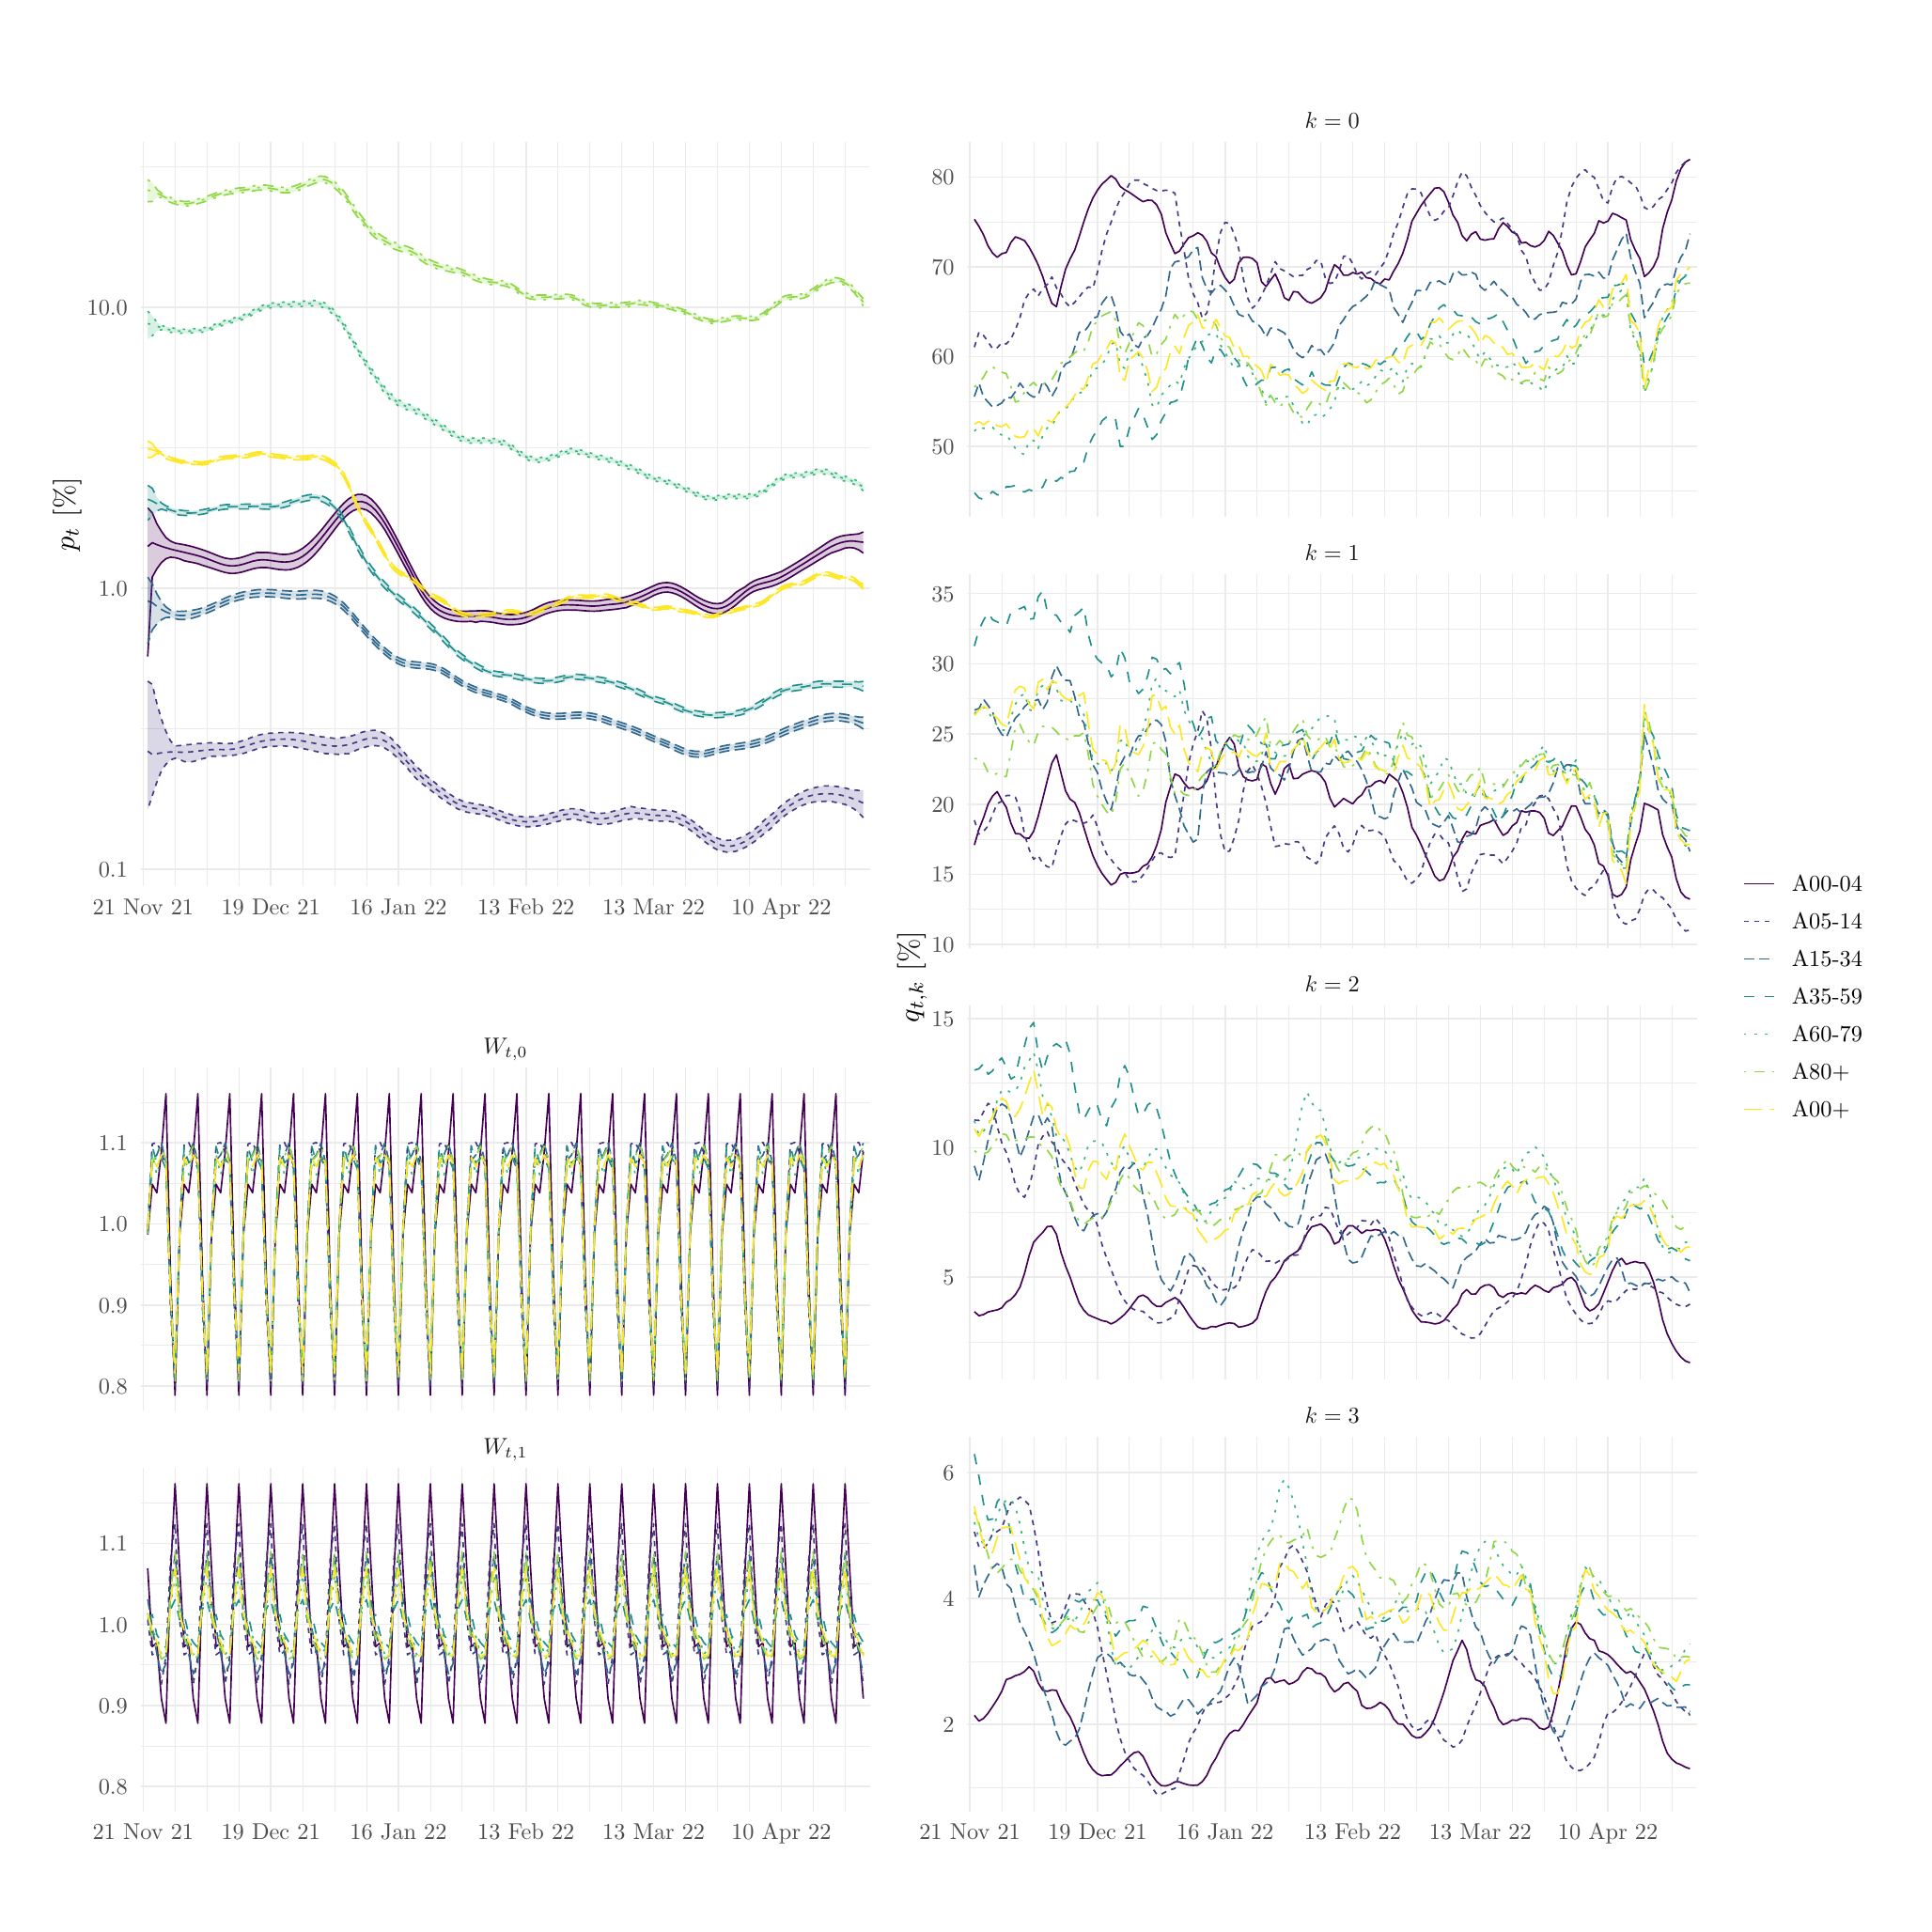
\begin{tikzpicture}[x=1pt,y=1pt]
\definecolor{fillColor}{RGB}{255,255,255}
\path[use as bounding box,fill=fillColor,fill opacity=0.00] (0,0) rectangle (722.70,722.70);
\begin{scope}
\path[clip] ( 44.06,392.04) rectangle (324.73,677.97);
\definecolor{drawColor}{gray}{0.92}

\path[draw=drawColor,line width= 0.3pt,line join=round] ( 44.06,452.41) --
	(324.73,452.41);

\path[draw=drawColor,line width= 0.3pt,line join=round] ( 44.06,560.44) --
	(324.73,560.44);

\path[draw=drawColor,line width= 0.3pt,line join=round] ( 44.06,668.48) --
	(324.73,668.48);

\path[draw=drawColor,line width= 0.3pt,line join=round] ( 57.32,392.04) --
	( 57.32,677.97);

\path[draw=drawColor,line width= 0.3pt,line join=round] ( 69.59,392.04) --
	( 69.59,677.97);

\path[draw=drawColor,line width= 0.3pt,line join=round] ( 81.86,392.04) --
	( 81.86,677.97);

\path[draw=drawColor,line width= 0.3pt,line join=round] (106.40,392.04) --
	(106.40,677.97);

\path[draw=drawColor,line width= 0.3pt,line join=round] (118.67,392.04) --
	(118.67,677.97);

\path[draw=drawColor,line width= 0.3pt,line join=round] (130.94,392.04) --
	(130.94,677.97);

\path[draw=drawColor,line width= 0.3pt,line join=round] (155.47,392.04) --
	(155.47,677.97);

\path[draw=drawColor,line width= 0.3pt,line join=round] (167.74,392.04) --
	(167.74,677.97);

\path[draw=drawColor,line width= 0.3pt,line join=round] (180.01,392.04) --
	(180.01,677.97);

\path[draw=drawColor,line width= 0.3pt,line join=round] (204.55,392.04) --
	(204.55,677.97);

\path[draw=drawColor,line width= 0.3pt,line join=round] (216.82,392.04) --
	(216.82,677.97);

\path[draw=drawColor,line width= 0.3pt,line join=round] (229.09,392.04) --
	(229.09,677.97);

\path[draw=drawColor,line width= 0.3pt,line join=round] (253.62,392.04) --
	(253.62,677.97);

\path[draw=drawColor,line width= 0.3pt,line join=round] (265.89,392.04) --
	(265.89,677.97);

\path[draw=drawColor,line width= 0.3pt,line join=round] (278.16,392.04) --
	(278.16,677.97);

\path[draw=drawColor,line width= 0.3pt,line join=round] (302.70,392.04) --
	(302.70,677.97);

\path[draw=drawColor,line width= 0.3pt,line join=round] (314.97,392.04) --
	(314.97,677.97);

\path[draw=drawColor,line width= 0.6pt,line join=round] ( 44.06,398.40) --
	(324.73,398.40);

\path[draw=drawColor,line width= 0.6pt,line join=round] ( 44.06,506.43) --
	(324.73,506.43);

\path[draw=drawColor,line width= 0.6pt,line join=round] ( 44.06,614.46) --
	(324.73,614.46);

\path[draw=drawColor,line width= 0.6pt,line join=round] ( 45.05,392.04) --
	( 45.05,677.97);

\path[draw=drawColor,line width= 0.6pt,line join=round] ( 94.13,392.04) --
	( 94.13,677.97);

\path[draw=drawColor,line width= 0.6pt,line join=round] (143.20,392.04) --
	(143.20,677.97);

\path[draw=drawColor,line width= 0.6pt,line join=round] (192.28,392.04) --
	(192.28,677.97);

\path[draw=drawColor,line width= 0.6pt,line join=round] (241.36,392.04) --
	(241.36,677.97);

\path[draw=drawColor,line width= 0.6pt,line join=round] (290.43,392.04) --
	(290.43,677.97);
\definecolor{drawColor}{RGB}{68,1,84}

\path[draw=drawColor,line width= 0.6pt,line join=round] ( 46.81,522.53) --
	( 48.56,524.01) --
	( 50.31,523.26) --
	( 52.06,522.63) --
	( 53.82,522.06) --
	( 55.57,521.56) --
	( 57.32,521.11) --
	( 59.08,520.70) --
	( 60.83,520.30) --
	( 62.58,519.87) --
	( 64.33,519.46) --
	( 66.09,519.00) --
	( 67.84,518.48) --
	( 69.59,517.87) --
	( 71.34,517.20) --
	( 73.10,516.52) --
	( 74.85,515.88) --
	( 76.60,515.38) --
	( 78.36,515.12) --
	( 80.11,515.10) --
	( 81.86,515.33) --
	( 83.61,515.76) --
	( 85.37,516.32) --
	( 87.12,516.86) --
	( 88.87,517.25) --
	( 90.62,517.42) --
	( 92.38,517.37) --
	( 94.13,517.16) --
	( 95.88,516.89) --
	( 97.63,516.66) --
	( 99.39,516.55) --
	(101.14,516.67) --
	(102.89,517.03) --
	(104.65,517.74) --
	(106.40,518.73) --
	(108.15,520.04) --
	(109.90,521.64) --
	(111.66,523.51) --
	(113.41,525.57) --
	(115.16,527.74) --
	(116.91,529.98) --
	(118.67,532.20) --
	(120.42,534.33) --
	(122.17,536.26) --
	(123.93,537.87) --
	(125.68,539.09) --
	(127.43,539.74) --
	(129.18,539.81) --
	(130.94,539.28) --
	(132.69,538.13) --
	(134.44,536.44) --
	(136.19,534.21) --
	(137.95,531.56) --
	(139.70,528.58) --
	(141.45,525.42) --
	(143.20,522.17) --
	(144.96,518.84) --
	(146.71,515.43) --
	(148.46,512.01) --
	(150.22,508.70) --
	(151.97,505.68) --
	(153.72,503.05) --
	(155.47,500.90) --
	(157.23,499.25) --
	(158.98,498.03) --
	(160.73,497.14) --
	(162.48,496.49) --
	(164.24,496.05) --
	(165.99,495.78) --
	(167.74,495.69) --
	(169.50,495.68) --
	(171.25,495.72) --
	(173.00,495.76) --
	(174.75,495.77) --
	(176.51,495.70) --
	(178.26,495.53) --
	(180.01,495.25) --
	(181.76,494.93) --
	(183.52,494.66) --
	(185.27,494.51) --
	(187.02,494.52) --
	(188.77,494.61) --
	(190.53,494.86) --
	(192.28,495.31) --
	(194.03,495.96) --
	(195.79,496.75) --
	(197.54,497.60) --
	(199.29,498.36) --
	(201.04,498.97) --
	(202.80,499.47) --
	(204.55,499.83) --
	(206.30,500.04) --
	(208.05,500.12) --
	(209.81,500.09) --
	(211.56,500.01) --
	(213.31,499.91) --
	(215.07,499.77) --
	(216.82,499.65) --
	(218.57,499.63) --
	(220.32,499.74) --
	(222.08,499.97) --
	(223.83,500.19) --
	(225.58,500.34) --
	(227.33,500.49) --
	(229.09,500.76) --
	(230.84,501.18) --
	(232.59,501.73) --
	(234.34,502.38) --
	(236.10,503.08) --
	(237.85,503.84) --
	(239.60,504.69) --
	(241.36,505.55) --
	(243.11,506.27) --
	(244.86,506.75) --
	(246.61,506.87) --
	(248.37,506.60) --
	(250.12,506.04) --
	(251.87,505.22) --
	(253.62,504.23) --
	(255.38,503.13) --
	(257.13,501.98) --
	(258.88,500.90) --
	(260.64,499.96) --
	(262.39,499.24) --
	(264.14,498.77) --
	(265.89,498.63) --
	(267.65,498.93) --
	(269.40,499.66) --
	(271.15,500.75) --
	(272.90,502.11) --
	(274.66,503.59) --
	(276.41,505.04) --
	(278.16,506.32) --
	(279.91,507.32) --
	(281.67,507.99) --
	(283.42,508.47) --
	(285.17,508.90) --
	(286.93,509.39) --
	(288.68,510.03) --
	(290.43,510.84) --
	(292.18,511.79) --
	(293.94,512.83) --
	(295.69,513.89) --
	(297.44,514.97) --
	(299.19,516.03) --
	(300.95,517.16) --
	(302.70,518.27) --
	(304.45,519.35) --
	(306.21,520.44) --
	(307.96,521.55) --
	(309.71,522.53) --
	(311.46,523.34) --
	(313.22,523.98) --
	(314.97,524.42) --
	(316.72,524.64) --
	(318.47,524.61) --
	(320.23,524.39) --
	(321.98,524.16);
\definecolor{drawColor}{RGB}{68,58,131}

\path[draw=drawColor,line width= 0.6pt,dash pattern=on 2pt off 2pt ,line join=round] ( 46.81,443.83) --
	( 48.56,442.57) --
	( 50.31,442.86) --
	( 52.06,443.20) --
	( 53.82,443.43) --
	( 55.57,443.52) --
	( 57.32,443.51) --
	( 59.08,443.46) --
	( 60.83,443.45) --
	( 62.58,443.51) --
	( 64.33,443.65) --
	( 66.09,443.88) --
	( 67.84,444.10) --
	( 69.59,444.29) --
	( 71.34,444.42) --
	( 73.10,444.48) --
	( 74.85,444.46) --
	( 76.60,444.45) --
	( 78.36,444.51) --
	( 80.11,444.69) --
	( 81.86,445.01) --
	( 83.61,445.48) --
	( 85.37,446.05) --
	( 87.12,446.67) --
	( 88.87,447.23) --
	( 90.62,447.65) --
	( 92.38,447.96) --
	( 94.13,448.17) --
	( 95.88,448.31) --
	( 97.63,448.43) --
	( 99.39,448.47) --
	(101.14,448.42) --
	(102.89,448.28) --
	(104.65,448.06) --
	(106.40,447.75) --
	(108.15,447.41) --
	(109.90,447.06) --
	(111.66,446.71) --
	(113.41,446.37) --
	(115.16,446.09) --
	(116.91,445.88) --
	(118.67,445.79) --
	(120.42,445.84) --
	(122.17,446.01) --
	(123.93,446.32) --
	(125.68,446.82) --
	(127.43,447.42) --
	(129.18,448.05) --
	(130.94,448.57) --
	(132.69,448.88) --
	(134.44,448.89) --
	(136.19,448.55) --
	(137.95,447.80) --
	(139.70,446.62) --
	(141.45,445.11) --
	(143.20,443.36) --
	(144.96,441.49) --
	(146.71,439.57) --
	(148.46,437.64) --
	(150.22,435.77) --
	(151.97,434.02) --
	(153.72,432.41) --
	(155.47,430.95) --
	(157.23,429.56) --
	(158.98,428.26) --
	(160.73,426.99) --
	(162.48,425.75) --
	(164.24,424.57) --
	(165.99,423.58) --
	(167.74,422.84) --
	(169.50,422.34) --
	(171.25,422.01) --
	(173.00,421.74) --
	(174.75,421.42) --
	(176.51,421.01) --
	(178.26,420.48) --
	(180.01,419.89) --
	(181.76,419.24) --
	(183.52,418.59) --
	(185.27,417.98) --
	(187.02,417.45) --
	(188.77,417.06) --
	(190.53,416.81) --
	(192.28,416.70) --
	(194.03,416.70) --
	(195.79,416.83) --
	(197.54,417.08) --
	(199.29,417.44) --
	(201.04,417.88) --
	(202.80,418.37) --
	(204.55,418.84) --
	(206.30,419.28) --
	(208.05,419.59) --
	(209.81,419.71) --
	(211.56,419.57) --
	(213.31,419.25) --
	(215.07,418.81) --
	(216.82,418.36) --
	(218.57,417.99) --
	(220.32,417.80) --
	(222.08,417.84) --
	(223.83,418.09) --
	(225.58,418.50) --
	(227.33,418.96) --
	(229.09,419.40) --
	(230.84,419.78) --
	(232.59,420.03) --
	(234.34,420.08) --
	(236.10,419.94) --
	(237.85,419.69) --
	(239.60,419.42) --
	(241.36,419.23) --
	(243.11,419.11) --
	(244.86,419.05) --
	(246.61,418.96) --
	(248.37,418.73) --
	(250.12,418.29) --
	(251.87,417.65) --
	(253.62,416.78) --
	(255.38,415.68) --
	(257.13,414.36) --
	(258.88,412.92) --
	(260.64,411.49) --
	(262.39,410.16) --
	(264.14,409.05) --
	(265.89,408.17) --
	(267.65,407.57) --
	(269.40,407.29) --
	(271.15,407.33) --
	(272.90,407.66) --
	(274.66,408.27) --
	(276.41,409.09) --
	(278.16,410.13) --
	(279.91,411.34) --
	(281.67,412.69) --
	(283.42,414.16) --
	(285.17,415.69) --
	(286.93,417.25) --
	(288.68,418.86) --
	(290.43,420.39) --
	(292.18,421.81) --
	(293.94,423.06) --
	(295.69,424.17) --
	(297.44,425.13) --
	(299.19,425.91) --
	(300.95,426.53) --
	(302.70,426.95) --
	(304.45,427.24) --
	(306.21,427.42) --
	(307.96,427.48) --
	(309.71,427.44) --
	(311.46,427.27) --
	(313.22,426.97) --
	(314.97,426.56) --
	(316.72,426.03) --
	(318.47,425.38) --
	(320.23,424.65) --
	(321.98,423.88);
\definecolor{drawColor}{RGB}{49,104,142}

\path[draw=drawColor,line width= 0.6pt,dash pattern=on 4pt off 2pt ,line join=round] ( 46.81,501.61) --
	( 48.56,500.92) --
	( 50.31,499.53) --
	( 52.06,498.35) --
	( 53.82,497.39) --
	( 55.57,496.68) --
	( 57.32,496.23) --
	( 59.08,496.02) --
	( 60.83,496.03) --
	( 62.58,496.23) --
	( 64.33,496.58) --
	( 66.09,497.04) --
	( 67.84,497.61) --
	( 69.59,498.27) --
	( 71.34,499.00) --
	( 73.10,499.81) --
	( 74.85,500.64) --
	( 76.60,501.44) --
	( 78.36,502.16) --
	( 80.11,502.78) --
	( 81.86,503.30) --
	( 83.61,503.73) --
	( 85.37,504.08) --
	( 87.12,504.35) --
	( 88.87,504.52) --
	( 90.62,504.62) --
	( 92.38,504.64) --
	( 94.13,504.59) --
	( 95.88,504.47) --
	( 97.63,504.31) --
	( 99.39,504.14) --
	(101.14,503.99) --
	(102.89,503.90) --
	(104.65,503.89) --
	(106.40,503.96) --
	(108.15,504.08) --
	(109.90,504.18) --
	(111.66,504.18) --
	(113.41,504.01) --
	(115.16,503.61) --
	(116.91,502.98) --
	(118.67,502.09) --
	(120.42,500.90) --
	(122.17,499.40) --
	(123.93,497.60) --
	(125.68,495.60) --
	(127.43,493.50) --
	(129.18,491.41) --
	(130.94,489.38) --
	(132.69,487.45) --
	(134.44,485.64) --
	(136.19,483.93) --
	(137.95,482.34) --
	(139.70,480.88) --
	(141.45,479.60) --
	(143.20,478.60) --
	(144.96,477.87) --
	(146.71,477.41) --
	(148.46,477.14) --
	(150.22,476.96) --
	(151.97,476.81) --
	(153.72,476.65) --
	(155.47,476.40) --
	(157.23,475.99) --
	(158.98,475.35) --
	(160.73,474.46) --
	(162.48,473.36) --
	(164.24,472.17) --
	(165.99,471.00) --
	(167.74,469.93) --
	(169.50,468.97) --
	(171.25,468.13) --
	(173.00,467.42) --
	(174.75,466.82) --
	(176.51,466.29) --
	(178.26,465.79) --
	(180.01,465.27) --
	(181.76,464.75) --
	(183.52,464.21) --
	(185.27,463.55) --
	(187.02,462.73) --
	(188.77,461.78) --
	(190.53,460.80) --
	(192.28,459.89) --
	(194.03,459.12) --
	(195.79,458.48) --
	(197.54,457.97) --
	(199.29,457.59) --
	(201.04,457.35) --
	(202.80,457.24) --
	(204.55,457.24) --
	(206.30,457.31) --
	(208.05,457.44) --
	(209.81,457.57) --
	(211.56,457.67) --
	(213.31,457.69) --
	(215.07,457.60) --
	(216.82,457.39) --
	(218.57,457.06) --
	(220.32,456.63) --
	(222.08,456.12) --
	(223.83,455.53) --
	(225.58,454.90) --
	(227.33,454.27) --
	(229.09,453.67) --
	(230.84,453.08) --
	(232.59,452.48) --
	(234.34,451.82) --
	(236.10,451.06) --
	(237.85,450.25) --
	(239.60,449.43) --
	(241.36,448.66) --
	(243.11,447.94) --
	(244.86,447.25) --
	(246.61,446.53) --
	(248.37,445.77) --
	(250.12,444.98) --
	(251.87,444.22) --
	(253.62,443.55) --
	(255.38,443.04) --
	(257.13,442.73) --
	(258.88,442.67) --
	(260.64,442.84) --
	(262.39,443.18) --
	(264.14,443.65) --
	(265.89,444.16) --
	(267.65,444.64) --
	(269.40,445.00) --
	(271.15,445.27) --
	(272.90,445.50) --
	(274.66,445.75) --
	(276.41,446.02) --
	(278.16,446.35) --
	(279.91,446.73) --
	(281.67,447.20) --
	(283.42,447.77) --
	(285.17,448.43) --
	(286.93,449.18) --
	(288.68,450.00) --
	(290.43,450.82) --
	(292.18,451.60) --
	(293.94,452.31) --
	(295.69,452.97) --
	(297.44,453.60) --
	(299.19,454.22) --
	(300.95,454.83) --
	(302.70,455.42) --
	(304.45,455.95) --
	(306.21,456.39) --
	(307.96,456.72) --
	(309.71,456.91) --
	(311.46,456.96) --
	(313.22,456.86) --
	(314.97,456.64) --
	(316.72,456.29) --
	(318.47,455.81) --
	(320.23,455.23) --
	(321.98,454.63);
\definecolor{drawColor}{RGB}{33,144,140}

\path[draw=drawColor,line width= 0.6pt,dash pattern=on 4pt off 4pt ,line join=round] ( 46.81,540.72) --
	( 48.56,540.02) --
	( 50.31,539.05) --
	( 52.06,538.13) --
	( 53.82,537.28) --
	( 55.57,536.55) --
	( 57.32,535.99) --
	( 59.08,535.60) --
	( 60.83,535.41) --
	( 62.58,535.38) --
	( 64.33,535.45) --
	( 66.09,535.59) --
	( 67.84,535.82) --
	( 69.59,536.17) --
	( 71.34,536.61) --
	( 73.10,537.10) --
	( 74.85,537.53) --
	( 76.60,537.76) --
	( 78.36,537.85) --
	( 80.11,537.87) --
	( 81.86,537.88) --
	( 83.61,537.88) --
	( 85.37,537.92) --
	( 87.12,537.97) --
	( 88.87,537.98) --
	( 90.62,537.92) --
	( 92.38,537.85) --
	( 94.13,537.84) --
	( 95.88,537.94) --
	( 97.63,538.22) --
	( 99.39,538.65) --
	(101.14,539.17) --
	(102.89,539.75) --
	(104.65,540.33) --
	(106.40,540.84) --
	(108.15,541.23) --
	(109.90,541.48) --
	(111.66,541.47) --
	(113.41,541.09) --
	(115.16,540.33) --
	(116.91,539.18) --
	(118.67,537.60) --
	(120.42,535.49) --
	(122.17,532.81) --
	(123.93,529.62) --
	(125.68,526.12) --
	(127.43,522.63) --
	(129.18,519.40) --
	(130.94,516.52) --
	(132.69,513.98) --
	(134.44,511.69) --
	(136.19,509.59) --
	(137.95,507.65) --
	(139.70,505.89) --
	(141.45,504.30) --
	(143.20,502.85) --
	(144.96,501.46) --
	(146.71,500.07) --
	(148.46,498.64) --
	(150.22,497.08) --
	(151.97,495.39) --
	(153.72,493.65) --
	(155.47,491.95) --
	(157.23,490.28) --
	(158.98,488.58) --
	(160.73,486.76) --
	(162.48,484.88) --
	(164.24,483.08) --
	(165.99,481.46) --
	(167.74,480.08) --
	(169.50,478.87) --
	(171.25,477.77) --
	(173.00,476.75) --
	(174.75,475.78) --
	(176.51,474.91) --
	(178.26,474.23) --
	(180.01,473.75) --
	(181.76,473.44) --
	(183.52,473.27) --
	(185.27,473.10) --
	(187.02,472.84) --
	(188.77,472.48) --
	(190.53,472.09) --
	(192.28,471.69) --
	(194.03,471.35) --
	(195.79,471.09) --
	(197.54,470.92) --
	(199.29,470.85) --
	(201.04,470.90) --
	(202.80,471.07) --
	(204.55,471.37) --
	(206.30,471.76) --
	(208.05,472.16) --
	(209.81,472.42) --
	(211.56,472.45) --
	(213.31,472.34) --
	(215.07,472.14) --
	(216.82,471.91) --
	(218.57,471.65) --
	(220.32,471.39) --
	(222.08,471.07) --
	(223.83,470.69) --
	(225.58,470.23) --
	(227.33,469.73) --
	(229.09,469.16) --
	(230.84,468.53) --
	(232.59,467.83) --
	(234.34,467.11) --
	(236.10,466.33) --
	(237.85,465.52) --
	(239.60,464.73) --
	(241.36,464.06) --
	(243.11,463.52) --
	(244.86,463.02) --
	(246.61,462.43) --
	(248.37,461.67) --
	(250.12,460.84) --
	(251.87,460.09) --
	(253.62,459.47) --
	(255.38,458.96) --
	(257.13,458.54) --
	(258.88,458.20) --
	(260.64,457.93) --
	(262.39,457.75) --
	(264.14,457.66) --
	(265.89,457.68) --
	(267.65,457.77) --
	(269.40,457.89) --
	(271.15,458.07) --
	(272.90,458.34) --
	(274.66,458.72) --
	(276.41,459.25) --
	(278.16,459.95) --
	(279.91,460.74) --
	(281.67,461.64) --
	(283.42,462.69) --
	(285.17,463.83) --
	(286.93,464.94) --
	(288.68,465.93) --
	(290.43,466.77) --
	(292.18,467.41) --
	(293.94,467.83) --
	(295.69,468.12) --
	(297.44,468.35) --
	(299.19,468.61) --
	(300.95,468.94) --
	(302.70,469.27) --
	(304.45,469.54) --
	(306.21,469.69) --
	(307.96,469.71) --
	(309.71,469.65) --
	(311.46,469.58) --
	(313.22,469.57) --
	(314.97,469.60) --
	(316.72,469.58) --
	(318.47,469.41) --
	(320.23,469.11) --
	(321.98,468.80);
\definecolor{drawColor}{RGB}{53,183,121}

\path[draw=drawColor,line width= 0.6pt,dash pattern=on 1pt off 3pt ,line join=round] ( 46.81,608.27) --
	( 48.56,607.87) --
	( 50.31,607.25) --
	( 52.06,606.69) --
	( 53.82,606.19) --
	( 55.57,605.82) --
	( 57.32,605.56) --
	( 59.08,605.37) --
	( 60.83,605.29) --
	( 62.58,605.37) --
	( 64.33,605.52) --
	( 66.09,605.61) --
	( 67.84,605.75) --
	( 69.59,606.09) --
	( 71.34,606.65) --
	( 73.10,607.39) --
	( 74.85,608.11) --
	( 76.60,608.66) --
	( 78.36,609.15) --
	( 80.11,609.65) --
	( 81.86,610.20) --
	( 83.61,610.77) --
	( 85.37,611.54) --
	( 87.12,612.51) --
	( 88.87,613.44) --
	( 90.62,614.25) --
	( 92.38,614.86) --
	( 94.13,615.23) --
	( 95.88,615.42) --
	( 97.63,615.55) --
	( 99.39,615.62) --
	(101.14,615.66) --
	(102.89,615.70) --
	(104.65,615.76) --
	(106.40,615.86) --
	(108.15,615.96) --
	(109.90,616.08) --
	(111.66,616.10) --
	(113.41,615.79) --
	(115.16,615.04) --
	(116.91,613.83) --
	(118.67,612.19) --
	(120.42,610.10) --
	(122.17,607.59) --
	(123.93,604.69) --
	(125.68,601.56) --
	(127.43,598.44) --
	(129.18,595.50) --
	(130.94,592.75) --
	(132.69,590.13) --
	(134.44,587.56) --
	(136.19,585.03) --
	(137.95,582.68) --
	(139.70,580.65) --
	(141.45,579.04) --
	(143.20,577.84) --
	(144.96,576.95) --
	(146.71,576.23) --
	(148.46,575.50) --
	(150.22,574.66) --
	(151.97,573.65) --
	(153.72,572.55) --
	(155.47,571.44) --
	(157.23,570.34) --
	(158.98,569.26) --
	(160.73,568.14) --
	(162.48,566.92) --
	(164.24,565.73) --
	(165.99,564.69) --
	(167.74,563.93) --
	(169.50,563.47) --
	(171.25,563.26) --
	(173.00,563.23) --
	(174.75,563.26) --
	(176.51,563.28) --
	(178.26,563.27) --
	(180.01,563.17) --
	(181.76,562.92) --
	(183.52,562.45) --
	(185.27,561.69) --
	(187.02,560.57) --
	(188.77,559.26) --
	(190.53,558.02) --
	(192.28,557.01) --
	(194.03,556.31) --
	(195.79,555.90) --
	(197.54,555.82) --
	(199.29,556.05) --
	(201.04,556.50) --
	(202.80,557.10) --
	(204.55,557.77) --
	(206.30,558.47) --
	(208.05,559.09) --
	(209.81,559.38) --
	(211.56,559.21) --
	(213.31,558.72) --
	(215.07,558.18) --
	(216.82,557.69) --
	(218.57,557.25) --
	(220.32,556.86) --
	(222.08,556.49) --
	(223.83,556.05) --
	(225.58,555.54) --
	(227.33,554.94) --
	(229.09,554.27) --
	(230.84,553.58) --
	(232.59,552.90) --
	(234.34,552.17) --
	(236.10,551.26) --
	(237.85,550.26) --
	(239.60,549.37) --
	(241.36,548.70) --
	(243.11,548.24) --
	(244.86,547.87) --
	(246.61,547.43) --
	(248.37,546.82) --
	(250.12,546.08) --
	(251.87,545.30) --
	(253.62,544.58) --
	(255.38,543.83) --
	(257.13,543.02) --
	(258.88,542.24) --
	(260.64,541.60) --
	(262.39,541.17) --
	(264.14,541.09) --
	(265.89,541.30) --
	(267.65,541.56) --
	(269.40,541.76) --
	(271.15,541.85) --
	(272.90,541.79) --
	(274.66,541.71) --
	(276.41,541.73) --
	(278.16,541.90) --
	(279.91,542.21) --
	(281.67,542.76) --
	(283.42,543.66) --
	(285.17,544.94) --
	(286.93,546.36) --
	(288.68,547.67) --
	(290.43,548.73) --
	(292.18,549.42) --
	(293.94,549.76) --
	(295.69,549.93) --
	(297.44,549.97) --
	(299.19,550.12) --
	(300.95,550.53) --
	(302.70,551.03) --
	(304.45,551.40) --
	(306.21,551.47) --
	(307.96,551.17) --
	(309.71,550.55) --
	(311.46,549.78) --
	(313.22,549.09) --
	(314.97,548.60) --
	(316.72,548.11) --
	(318.47,547.40) --
	(320.23,546.44) --
	(321.98,545.47);
\definecolor{drawColor}{RGB}{143,215,68}

\path[draw=drawColor,line width= 0.6pt,dash pattern=on 1pt off 3pt on 4pt off 3pt ,line join=round] ( 46.81,659.61) --
	( 48.56,659.07) --
	( 50.31,658.39) --
	( 52.06,657.58) --
	( 53.82,656.65) --
	( 55.57,655.81) --
	( 57.32,655.15) --
	( 59.08,654.63) --
	( 60.83,654.34) --
	( 62.58,654.42) --
	( 64.33,654.79) --
	( 66.09,655.27) --
	( 67.84,655.79) --
	( 69.59,656.32) --
	( 71.34,656.93) --
	( 73.10,657.61) --
	( 74.85,658.18) --
	( 76.60,658.63) --
	( 78.36,659.00) --
	( 80.11,659.26) --
	( 81.86,659.48) --
	( 83.61,659.60) --
	( 85.37,659.82) --
	( 87.12,660.19) --
	( 88.87,660.51) --
	( 90.62,660.61) --
	( 92.38,660.50) --
	( 94.13,660.24) --
	( 95.88,659.94) --
	( 97.63,659.71) --
	( 99.39,659.60) --
	(101.14,659.66) --
	(102.89,659.99) --
	(104.65,660.58) --
	(106.40,661.35) --
	(108.15,662.15) --
	(109.90,662.94) --
	(111.66,663.56) --
	(113.41,663.80) --
	(115.16,663.55) --
	(116.91,662.82) --
	(118.67,661.63) --
	(120.42,660.02) --
	(122.17,658.02) --
	(123.93,655.64) --
	(125.68,653.08) --
	(127.43,650.53) --
	(129.18,648.12) --
	(130.94,645.93) --
	(132.69,644.02) --
	(134.44,642.42) --
	(136.19,641.12) --
	(137.95,640.01) --
	(139.70,639.05) --
	(141.45,638.27) --
	(143.20,637.65) --
	(144.96,637.14) --
	(146.71,636.60) --
	(148.46,635.87) --
	(150.22,634.87) --
	(151.97,633.69) --
	(153.72,632.51) --
	(155.47,631.53) --
	(157.23,630.77) --
	(158.98,630.22) --
	(160.73,629.82) --
	(162.48,629.44) --
	(164.24,629.05) --
	(165.99,628.56) --
	(167.74,627.95) --
	(169.50,627.24) --
	(171.25,626.49) --
	(173.00,625.81) --
	(174.75,625.18) --
	(176.51,624.67) --
	(178.26,624.28) --
	(180.01,624.07) --
	(181.76,623.96) --
	(183.52,623.79) --
	(185.27,623.30) --
	(187.02,622.38) --
	(188.77,621.17) --
	(190.53,620.04) --
	(192.28,619.15) --
	(194.03,618.61) --
	(195.79,618.37) --
	(197.54,618.34) --
	(199.29,618.37) --
	(201.04,618.46) --
	(202.80,618.56) --
	(204.55,618.63) --
	(206.30,618.67) --
	(208.05,618.67) --
	(209.81,618.41) --
	(211.56,617.83) --
	(213.31,616.98) --
	(215.07,616.14) --
	(216.82,615.53) --
	(218.57,615.18) --
	(220.32,615.10) --
	(222.08,615.24) --
	(223.83,615.39) --
	(225.58,615.42) --
	(227.33,615.40) --
	(229.09,615.40) --
	(230.84,615.51) --
	(232.59,615.83) --
	(234.34,616.21) --
	(236.10,616.35) --
	(237.85,616.24) --
	(239.60,615.92) --
	(241.36,615.54) --
	(243.11,615.24) --
	(244.86,615.01) --
	(246.61,614.77) --
	(248.37,614.37) --
	(250.12,613.78) --
	(251.87,613.18) --
	(253.62,612.61) --
	(255.38,611.95) --
	(257.13,611.23) --
	(258.88,610.52) --
	(260.64,609.81) --
	(262.39,609.26) --
	(264.14,609.08) --
	(265.89,609.29) --
	(267.65,609.65) --
	(269.40,609.99) --
	(271.15,610.27) --
	(272.90,610.43) --
	(274.66,610.42) --
	(276.41,610.29) --
	(278.16,610.25) --
	(279.91,610.31) --
	(281.67,610.65) --
	(283.42,611.51) --
	(285.17,612.89) --
	(286.93,614.54) --
	(288.68,616.15) --
	(290.43,617.41) --
	(292.18,618.16) --
	(293.94,618.45) --
	(295.69,618.55) --
	(297.44,618.64) --
	(299.19,618.98) --
	(300.95,619.78) --
	(302.70,620.88) --
	(304.45,622.05) --
	(306.21,623.21) --
	(307.96,624.28) --
	(309.71,624.94) --
	(311.46,625.02) --
	(313.22,624.60) --
	(314.97,623.89) --
	(316.72,622.79) --
	(318.47,621.08) --
	(320.23,618.83) --
	(321.98,616.44);
\definecolor{drawColor}{RGB}{253,231,37}

\path[draw=drawColor,line width= 0.6pt,dash pattern=on 7pt off 3pt ,line join=round] ( 46.81,560.14) --
	( 48.56,559.75) --
	( 50.31,559.10) --
	( 52.06,558.16) --
	( 53.82,557.06) --
	( 55.57,556.28) --
	( 57.32,555.79) --
	( 59.08,555.28) --
	( 60.83,554.91) --
	( 62.58,554.76) --
	( 64.33,554.72) --
	( 66.09,554.58) --
	( 67.84,554.50) --
	( 69.59,554.69) --
	( 71.34,555.13) --
	( 73.10,555.89) --
	( 74.85,556.51) --
	( 76.60,556.77) --
	( 78.36,556.92) --
	( 80.11,557.06) --
	( 81.86,557.21) --
	( 83.61,557.18) --
	( 85.37,557.40) --
	( 87.12,557.96) --
	( 88.87,558.27) --
	( 90.62,558.23) --
	( 92.38,558.01) --
	( 94.13,557.67) --
	( 95.88,557.34) --
	( 97.63,557.15) --
	( 99.39,556.98) --
	(101.14,556.72) --
	(102.89,556.58) --
	(104.65,556.53) --
	(106.40,556.63) --
	(108.15,556.70) --
	(109.90,556.94) --
	(111.66,557.15) --
	(113.41,556.92) --
	(115.16,556.26) --
	(116.91,555.40) --
	(118.67,554.26) --
	(120.42,552.54) --
	(122.17,550.00) --
	(123.93,546.38) --
	(125.68,542.10) --
	(127.43,537.94) --
	(129.18,534.43) --
	(130.94,531.49) --
	(132.69,528.77) --
	(134.44,525.86) --
	(136.19,522.62) --
	(137.95,519.41) --
	(139.70,516.50) --
	(141.45,514.26) --
	(143.20,512.73) --
	(144.96,511.73) --
	(146.71,510.93) --
	(148.46,509.97) --
	(150.22,508.55) --
	(151.97,506.82) --
	(153.72,505.24) --
	(155.47,504.05) --
	(157.23,503.22) --
	(158.98,502.44) --
	(160.73,501.43) --
	(162.48,499.98) --
	(164.24,498.53) --
	(165.99,497.33) --
	(167.74,496.58) --
	(169.50,496.13) --
	(171.25,495.95) --
	(173.00,496.06) --
	(174.75,496.20) --
	(176.51,496.29) --
	(178.26,496.37) --
	(180.01,496.48) --
	(181.76,496.71) --
	(183.52,497.22) --
	(185.27,497.67) --
	(187.02,497.65) --
	(188.77,497.28) --
	(190.53,496.89) --
	(192.28,496.68) --
	(194.03,496.74) --
	(195.79,497.16) --
	(197.54,497.86) --
	(199.29,498.64) --
	(201.04,499.40) --
	(202.80,500.08) --
	(204.55,500.71) --
	(206.30,501.45) --
	(208.05,502.41) --
	(209.81,503.10) --
	(211.56,503.36) --
	(213.31,503.31) --
	(215.07,503.24) --
	(216.82,503.26) --
	(218.57,503.28) --
	(220.32,503.44) --
	(222.08,503.69) --
	(223.83,503.59) --
	(225.58,503.08) --
	(227.33,502.35) --
	(229.09,501.64) --
	(230.84,501.10) --
	(232.59,500.82) --
	(234.34,500.64) --
	(236.10,500.08) --
	(237.85,499.43) --
	(239.60,498.85) --
	(241.36,498.58) --
	(243.11,498.67) --
	(244.86,498.99) --
	(246.61,499.14) --
	(248.37,498.87) --
	(250.12,498.35) --
	(251.87,497.93) --
	(253.62,497.72) --
	(255.38,497.42) --
	(257.13,496.98) --
	(258.88,496.56) --
	(260.64,496.07) --
	(262.39,495.69) --
	(264.14,495.69) --
	(265.89,496.17) --
	(267.65,496.71) --
	(269.40,497.15) --
	(271.15,497.66) --
	(272.90,498.12) --
	(274.66,498.56) --
	(276.41,498.98) --
	(278.16,499.52) --
	(279.91,499.89) --
	(281.67,500.28) --
	(283.42,501.06) --
	(285.17,502.31) --
	(286.93,503.77) --
	(288.68,505.19) --
	(290.43,506.41) --
	(292.18,507.22) --
	(293.94,507.63) --
	(295.69,508.01) --
	(297.44,508.28) --
	(299.19,508.77) --
	(300.95,509.68) --
	(302.70,510.70) --
	(304.45,511.50) --
	(306.21,511.99) --
	(307.96,512.11) --
	(309.71,511.68) --
	(311.46,511.00) --
	(313.22,510.54) --
	(314.97,510.57) --
	(316.72,510.57) --
	(318.47,509.84) --
	(320.23,508.38) --
	(321.98,507.03);
\definecolor{fillColor}{RGB}{68,1,84}

\path[fill=fillColor,fill opacity=0.20] ( 46.81,537.39) --
	( 48.56,535.49) --
	( 50.31,531.30) --
	( 52.06,528.42) --
	( 53.82,525.95) --
	( 55.57,524.63) --
	( 57.32,523.84) --
	( 59.08,523.51) --
	( 60.83,523.22) --
	( 62.58,522.83) --
	( 64.33,522.39) --
	( 66.09,521.86) --
	( 67.84,521.30) --
	( 69.59,520.67) --
	( 71.34,519.99) --
	( 73.10,519.27) --
	( 74.85,518.61) --
	( 76.60,518.07) --
	( 78.36,517.79) --
	( 80.11,517.82) --
	( 81.86,518.10) --
	( 83.61,518.57) --
	( 85.37,519.15) --
	( 87.12,519.80) --
	( 88.87,520.23) --
	( 90.62,520.24) --
	( 92.38,520.25) --
	( 94.13,520.10) --
	( 95.88,519.87) --
	( 97.63,519.57) --
	( 99.39,519.46) --
	(101.14,519.63) --
	(102.89,520.05) --
	(104.65,520.80) --
	(106.40,521.85) --
	(108.15,523.19) --
	(109.90,524.79) --
	(111.66,526.64) --
	(113.41,528.64) --
	(115.16,530.81) --
	(116.91,533.05) --
	(118.67,535.18) --
	(120.42,537.26) --
	(122.17,539.16) --
	(123.93,540.75) --
	(125.68,541.84) --
	(127.43,542.56) --
	(129.18,542.60) --
	(130.94,542.04) --
	(132.69,540.80) --
	(134.44,539.04) --
	(136.19,536.78) --
	(137.95,534.09) --
	(139.70,531.06) --
	(141.45,527.81) --
	(143.20,524.50) --
	(144.96,521.10) --
	(146.71,517.67) --
	(148.46,514.21) --
	(150.22,510.88) --
	(151.97,507.83) --
	(153.72,505.20) --
	(155.47,503.16) --
	(157.23,501.46) --
	(158.98,500.15) --
	(160.73,499.19) --
	(162.48,498.49) --
	(164.24,497.97) --
	(165.99,497.75) --
	(167.74,497.64) --
	(169.50,497.66) --
	(171.25,497.74) --
	(173.00,497.78) --
	(174.75,497.85) --
	(176.51,497.83) --
	(178.26,497.65) --
	(180.01,497.18) --
	(181.76,496.87) --
	(183.52,496.57) --
	(185.27,496.41) --
	(187.02,496.37) --
	(188.77,496.51) --
	(190.53,496.78) --
	(192.28,497.20) --
	(194.03,497.83) --
	(195.79,498.67) --
	(197.54,499.58) --
	(199.29,500.39) --
	(201.04,501.02) --
	(202.80,501.39) --
	(204.55,501.71) --
	(206.30,501.96) --
	(208.05,502.00) --
	(209.81,501.99) --
	(211.56,501.89) --
	(213.31,501.79) --
	(215.07,501.63) --
	(216.82,501.56) --
	(218.57,501.57) --
	(220.32,501.69) --
	(222.08,501.96) --
	(223.83,502.23) --
	(225.58,502.35) --
	(227.33,502.49) --
	(229.09,502.77) --
	(230.84,503.20) --
	(232.59,503.71) --
	(234.34,504.39) --
	(236.10,505.04) --
	(237.85,505.80) --
	(239.60,506.63) --
	(241.36,507.41) --
	(243.11,508.18) --
	(244.86,508.56) --
	(246.61,508.68) --
	(248.37,508.43) --
	(250.12,507.86) --
	(251.87,507.04) --
	(253.62,506.05) --
	(255.38,504.94) --
	(257.13,503.78) --
	(258.88,502.76) --
	(260.64,501.86) --
	(262.39,501.17) --
	(264.14,500.68) --
	(265.89,500.55) --
	(267.65,500.81) --
	(269.40,501.87) --
	(271.15,503.21) --
	(272.90,504.83) --
	(274.66,505.96) --
	(276.41,506.92) --
	(278.16,508.27) --
	(279.91,509.28) --
	(281.67,509.99) --
	(283.42,510.51) --
	(285.17,510.98) --
	(286.93,511.60) --
	(288.68,512.21) --
	(290.43,512.88) --
	(292.18,513.86) --
	(293.94,514.89) --
	(295.69,515.95) --
	(297.44,517.03) --
	(299.19,518.12) --
	(300.95,519.27) --
	(302.70,520.38) --
	(304.45,521.54) --
	(306.21,522.72) --
	(307.96,523.91) --
	(309.71,524.98) --
	(311.46,525.85) --
	(313.22,526.48) --
	(314.97,526.82) --
	(316.72,527.05) --
	(318.47,527.21) --
	(320.23,527.40) --
	(321.98,528.15) --
	(321.98,520.01) --
	(320.23,521.23) --
	(318.47,521.96) --
	(316.72,522.15) --
	(314.97,521.95) --
	(313.22,521.25) --
	(311.46,520.65) --
	(309.71,520.07) --
	(307.96,519.17) --
	(306.21,518.09) --
	(304.45,517.07) --
	(302.70,515.99) --
	(300.95,514.93) --
	(299.19,513.91) --
	(297.44,512.85) --
	(295.69,511.75) --
	(293.94,510.68) --
	(292.18,509.67) --
	(290.43,508.77) --
	(288.68,507.97) --
	(286.93,507.31) --
	(285.17,506.82) --
	(283.42,506.39) --
	(281.67,505.92) --
	(279.91,505.31) --
	(278.16,504.31) --
	(276.41,503.03) --
	(274.66,501.55) --
	(272.90,500.00) --
	(271.15,498.69) --
	(269.40,497.65) --
	(267.65,496.88) --
	(265.89,496.65) --
	(264.14,496.82) --
	(262.39,497.30) --
	(260.64,498.01) --
	(258.88,498.93) --
	(257.13,500.02) --
	(255.38,501.20) --
	(253.62,502.35) --
	(251.87,503.37) --
	(250.12,504.19) --
	(248.37,504.76) --
	(246.61,505.03) --
	(244.86,504.89) --
	(243.11,504.41) --
	(241.36,503.71) --
	(239.60,502.76) --
	(237.85,501.92) --
	(236.10,501.15) --
	(234.34,500.40) --
	(232.59,499.75) --
	(230.84,499.02) --
	(229.09,498.78) --
	(227.33,498.50) --
	(225.58,498.28) --
	(223.83,498.13) --
	(222.08,497.95) --
	(220.32,497.76) --
	(218.57,497.66) --
	(216.82,497.68) --
	(215.07,497.81) --
	(213.31,497.95) --
	(211.56,498.10) --
	(209.81,498.11) --
	(208.05,498.14) --
	(206.30,498.05) --
	(204.55,497.87) --
	(202.80,497.50) --
	(201.04,497.02) --
	(199.29,496.41) --
	(197.54,495.65) --
	(195.79,494.79) --
	(194.03,493.98) --
	(192.28,493.29) --
	(190.53,492.81) --
	(188.77,492.59) --
	(187.02,492.48) --
	(185.27,492.47) --
	(183.52,492.68) --
	(181.76,492.94) --
	(180.01,493.29) --
	(178.26,493.53) --
	(176.51,493.69) --
	(174.75,493.78) --
	(173.00,493.39) --
	(171.25,493.77) --
	(169.50,493.67) --
	(167.74,493.66) --
	(165.99,493.73) --
	(164.24,494.04) --
	(162.48,494.44) --
	(160.73,495.06) --
	(158.98,495.93) --
	(157.23,497.12) --
	(155.47,498.75) --
	(153.72,500.86) --
	(151.97,503.47) --
	(150.22,506.45) --
	(148.46,509.69) --
	(146.71,513.06) --
	(144.96,516.26) --
	(143.20,519.58) --
	(141.45,522.79) --
	(139.70,525.93) --
	(137.95,529.01) --
	(136.19,531.58) --
	(134.44,533.69) --
	(132.69,535.46) --
	(130.94,536.59) --
	(129.18,537.09) --
	(127.43,536.96) --
	(125.68,536.24) --
	(123.93,535.03) --
	(122.17,533.38) --
	(120.42,531.37) --
	(118.67,529.11) --
	(116.91,526.79) --
	(115.16,524.49) --
	(113.41,522.27) --
	(111.66,520.20) --
	(109.90,518.32) --
	(108.15,516.80) --
	(106.40,515.57) --
	(104.65,514.60) --
	(102.89,513.96) --
	(101.14,513.57) --
	( 99.39,513.55) --
	( 97.63,513.66) --
	( 95.88,513.91) --
	( 94.13,514.22) --
	( 92.38,514.44) --
	( 90.62,514.47) --
	( 88.87,514.29) --
	( 87.12,513.92) --
	( 85.37,513.39) --
	( 83.61,512.86) --
	( 81.86,512.45) --
	( 80.11,512.21) --
	( 78.36,512.24) --
	( 76.60,512.54) --
	( 74.85,513.04) --
	( 73.10,513.63) --
	( 71.34,514.23) --
	( 69.59,514.77) --
	( 67.84,515.32) --
	( 66.09,515.95) --
	( 64.33,516.35) --
	( 62.58,516.68) --
	( 60.83,517.06) --
	( 59.08,517.79) --
	( 57.32,518.25) --
	( 55.57,518.43) --
	( 53.82,517.84) --
	( 52.06,516.35) --
	( 50.31,513.95) --
	( 48.56,510.79) --
	( 46.81,480.24) --
	cycle;
\definecolor{drawColor}{RGB}{68,1,84}

\path[draw=drawColor,line width= 0.6pt,line join=round] ( 46.81,537.39) --
	( 48.56,535.49) --
	( 50.31,531.30) --
	( 52.06,528.42) --
	( 53.82,525.95) --
	( 55.57,524.63) --
	( 57.32,523.84) --
	( 59.08,523.51) --
	( 60.83,523.22) --
	( 62.58,522.83) --
	( 64.33,522.39) --
	( 66.09,521.86) --
	( 67.84,521.30) --
	( 69.59,520.67) --
	( 71.34,519.99) --
	( 73.10,519.27) --
	( 74.85,518.61) --
	( 76.60,518.07) --
	( 78.36,517.79) --
	( 80.11,517.82) --
	( 81.86,518.10) --
	( 83.61,518.57) --
	( 85.37,519.15) --
	( 87.12,519.80) --
	( 88.87,520.23) --
	( 90.62,520.24) --
	( 92.38,520.25) --
	( 94.13,520.10) --
	( 95.88,519.87) --
	( 97.63,519.57) --
	( 99.39,519.46) --
	(101.14,519.63) --
	(102.89,520.05) --
	(104.65,520.80) --
	(106.40,521.85) --
	(108.15,523.19) --
	(109.90,524.79) --
	(111.66,526.64) --
	(113.41,528.64) --
	(115.16,530.81) --
	(116.91,533.05) --
	(118.67,535.18) --
	(120.42,537.26) --
	(122.17,539.16) --
	(123.93,540.75) --
	(125.68,541.84) --
	(127.43,542.56) --
	(129.18,542.60) --
	(130.94,542.04) --
	(132.69,540.80) --
	(134.44,539.04) --
	(136.19,536.78) --
	(137.95,534.09) --
	(139.70,531.06) --
	(141.45,527.81) --
	(143.20,524.50) --
	(144.96,521.10) --
	(146.71,517.67) --
	(148.46,514.21) --
	(150.22,510.88) --
	(151.97,507.83) --
	(153.72,505.20) --
	(155.47,503.16) --
	(157.23,501.46) --
	(158.98,500.15) --
	(160.73,499.19) --
	(162.48,498.49) --
	(164.24,497.97) --
	(165.99,497.75) --
	(167.74,497.64) --
	(169.50,497.66) --
	(171.25,497.74) --
	(173.00,497.78) --
	(174.75,497.85) --
	(176.51,497.83) --
	(178.26,497.65) --
	(180.01,497.18) --
	(181.76,496.87) --
	(183.52,496.57) --
	(185.27,496.41) --
	(187.02,496.37) --
	(188.77,496.51) --
	(190.53,496.78) --
	(192.28,497.20) --
	(194.03,497.83) --
	(195.79,498.67) --
	(197.54,499.58) --
	(199.29,500.39) --
	(201.04,501.02) --
	(202.80,501.39) --
	(204.55,501.71) --
	(206.30,501.96) --
	(208.05,502.00) --
	(209.81,501.99) --
	(211.56,501.89) --
	(213.31,501.79) --
	(215.07,501.63) --
	(216.82,501.56) --
	(218.57,501.57) --
	(220.32,501.69) --
	(222.08,501.96) --
	(223.83,502.23) --
	(225.58,502.35) --
	(227.33,502.49) --
	(229.09,502.77) --
	(230.84,503.20) --
	(232.59,503.71) --
	(234.34,504.39) --
	(236.10,505.04) --
	(237.85,505.80) --
	(239.60,506.63) --
	(241.36,507.41) --
	(243.11,508.18) --
	(244.86,508.56) --
	(246.61,508.68) --
	(248.37,508.43) --
	(250.12,507.86) --
	(251.87,507.04) --
	(253.62,506.05) --
	(255.38,504.94) --
	(257.13,503.78) --
	(258.88,502.76) --
	(260.64,501.86) --
	(262.39,501.17) --
	(264.14,500.68) --
	(265.89,500.55) --
	(267.65,500.81) --
	(269.40,501.87) --
	(271.15,503.21) --
	(272.90,504.83) --
	(274.66,505.96) --
	(276.41,506.92) --
	(278.16,508.27) --
	(279.91,509.28) --
	(281.67,509.99) --
	(283.42,510.51) --
	(285.17,510.98) --
	(286.93,511.60) --
	(288.68,512.21) --
	(290.43,512.88) --
	(292.18,513.86) --
	(293.94,514.89) --
	(295.69,515.95) --
	(297.44,517.03) --
	(299.19,518.12) --
	(300.95,519.27) --
	(302.70,520.38) --
	(304.45,521.54) --
	(306.21,522.72) --
	(307.96,523.91) --
	(309.71,524.98) --
	(311.46,525.85) --
	(313.22,526.48) --
	(314.97,526.82) --
	(316.72,527.05) --
	(318.47,527.21) --
	(320.23,527.40) --
	(321.98,528.15);

\path[draw=drawColor,line width= 0.6pt,line join=round] (321.98,520.01) --
	(320.23,521.23) --
	(318.47,521.96) --
	(316.72,522.15) --
	(314.97,521.95) --
	(313.22,521.25) --
	(311.46,520.65) --
	(309.71,520.07) --
	(307.96,519.17) --
	(306.21,518.09) --
	(304.45,517.07) --
	(302.70,515.99) --
	(300.95,514.93) --
	(299.19,513.91) --
	(297.44,512.85) --
	(295.69,511.75) --
	(293.94,510.68) --
	(292.18,509.67) --
	(290.43,508.77) --
	(288.68,507.97) --
	(286.93,507.31) --
	(285.17,506.82) --
	(283.42,506.39) --
	(281.67,505.92) --
	(279.91,505.31) --
	(278.16,504.31) --
	(276.41,503.03) --
	(274.66,501.55) --
	(272.90,500.00) --
	(271.15,498.69) --
	(269.40,497.65) --
	(267.65,496.88) --
	(265.89,496.65) --
	(264.14,496.82) --
	(262.39,497.30) --
	(260.64,498.01) --
	(258.88,498.93) --
	(257.13,500.02) --
	(255.38,501.20) --
	(253.62,502.35) --
	(251.87,503.37) --
	(250.12,504.19) --
	(248.37,504.76) --
	(246.61,505.03) --
	(244.86,504.89) --
	(243.11,504.41) --
	(241.36,503.71) --
	(239.60,502.76) --
	(237.85,501.92) --
	(236.10,501.15) --
	(234.34,500.40) --
	(232.59,499.75) --
	(230.84,499.02) --
	(229.09,498.78) --
	(227.33,498.50) --
	(225.58,498.28) --
	(223.83,498.13) --
	(222.08,497.95) --
	(220.32,497.76) --
	(218.57,497.66) --
	(216.82,497.68) --
	(215.07,497.81) --
	(213.31,497.95) --
	(211.56,498.10) --
	(209.81,498.11) --
	(208.05,498.14) --
	(206.30,498.05) --
	(204.55,497.87) --
	(202.80,497.50) --
	(201.04,497.02) --
	(199.29,496.41) --
	(197.54,495.65) --
	(195.79,494.79) --
	(194.03,493.98) --
	(192.28,493.29) --
	(190.53,492.81) --
	(188.77,492.59) --
	(187.02,492.48) --
	(185.27,492.47) --
	(183.52,492.68) --
	(181.76,492.94) --
	(180.01,493.29) --
	(178.26,493.53) --
	(176.51,493.69) --
	(174.75,493.78) --
	(173.00,493.39) --
	(171.25,493.77) --
	(169.50,493.67) --
	(167.74,493.66) --
	(165.99,493.73) --
	(164.24,494.04) --
	(162.48,494.44) --
	(160.73,495.06) --
	(158.98,495.93) --
	(157.23,497.12) --
	(155.47,498.75) --
	(153.72,500.86) --
	(151.97,503.47) --
	(150.22,506.45) --
	(148.46,509.69) --
	(146.71,513.06) --
	(144.96,516.26) --
	(143.20,519.58) --
	(141.45,522.79) --
	(139.70,525.93) --
	(137.95,529.01) --
	(136.19,531.58) --
	(134.44,533.69) --
	(132.69,535.46) --
	(130.94,536.59) --
	(129.18,537.09) --
	(127.43,536.96) --
	(125.68,536.24) --
	(123.93,535.03) --
	(122.17,533.38) --
	(120.42,531.37) --
	(118.67,529.11) --
	(116.91,526.79) --
	(115.16,524.49) --
	(113.41,522.27) --
	(111.66,520.20) --
	(109.90,518.32) --
	(108.15,516.80) --
	(106.40,515.57) --
	(104.65,514.60) --
	(102.89,513.96) --
	(101.14,513.57) --
	( 99.39,513.55) --
	( 97.63,513.66) --
	( 95.88,513.91) --
	( 94.13,514.22) --
	( 92.38,514.44) --
	( 90.62,514.47) --
	( 88.87,514.29) --
	( 87.12,513.92) --
	( 85.37,513.39) --
	( 83.61,512.86) --
	( 81.86,512.45) --
	( 80.11,512.21) --
	( 78.36,512.24) --
	( 76.60,512.54) --
	( 74.85,513.04) --
	( 73.10,513.63) --
	( 71.34,514.23) --
	( 69.59,514.77) --
	( 67.84,515.32) --
	( 66.09,515.95) --
	( 64.33,516.35) --
	( 62.58,516.68) --
	( 60.83,517.06) --
	( 59.08,517.79) --
	( 57.32,518.25) --
	( 55.57,518.43) --
	( 53.82,517.84) --
	( 52.06,516.35) --
	( 50.31,513.95) --
	( 48.56,510.79) --
	( 46.81,480.24);
\definecolor{fillColor}{RGB}{68,58,131}

\path[fill=fillColor,fill opacity=0.20] ( 46.81,470.75) --
	( 48.56,469.53) --
	( 50.31,462.27) --
	( 52.06,456.19) --
	( 53.82,451.44) --
	( 55.57,447.79) --
	( 57.32,445.87) --
	( 59.08,445.97) --
	( 60.83,446.26) --
	( 62.58,446.36) --
	( 64.33,446.51) --
	( 66.09,446.75) --
	( 67.84,446.81) --
	( 69.59,447.01) --
	( 71.34,447.03) --
	( 73.10,446.95) --
	( 74.85,446.84) --
	( 76.60,446.76) --
	( 78.36,446.76) --
	( 80.11,446.95) --
	( 81.86,447.40) --
	( 83.61,447.99) --
	( 85.37,448.57) --
	( 87.12,449.28) --
	( 88.87,449.87) --
	( 90.62,450.28) --
	( 92.38,450.65) --
	( 94.13,450.76) --
	( 95.88,450.78) --
	( 97.63,450.99) --
	( 99.39,450.99) --
	(101.14,451.02) --
	(102.89,450.95) --
	(104.65,450.83) --
	(106.40,450.66) --
	(108.15,450.37) --
	(109.90,450.11) --
	(111.66,449.81) --
	(113.41,449.40) --
	(115.16,449.22) --
	(116.91,448.99) --
	(118.67,448.77) --
	(120.42,448.87) --
	(122.17,449.14) --
	(123.93,449.43) --
	(125.68,449.84) --
	(127.43,450.47) --
	(129.18,451.11) --
	(130.94,451.56) --
	(132.69,451.78) --
	(134.44,451.88) --
	(136.19,451.38) --
	(137.95,450.59) --
	(139.70,449.49) --
	(141.45,447.77) --
	(143.20,445.86) --
	(144.96,443.93) --
	(146.71,441.79) --
	(148.46,439.83) --
	(150.22,437.86) --
	(151.97,436.25) --
	(153.72,434.49) --
	(155.47,433.13) --
	(157.23,431.72) --
	(158.98,430.32) --
	(160.73,429.04) --
	(162.48,427.68) --
	(164.24,426.47) --
	(165.99,425.48) --
	(167.74,424.69) --
	(169.50,424.18) --
	(171.25,423.83) --
	(173.00,423.56) --
	(174.75,423.22) --
	(176.51,422.86) --
	(178.26,422.40) --
	(180.01,421.74) --
	(181.76,421.07) --
	(183.52,420.43) --
	(185.27,419.83) --
	(187.02,419.24) --
	(188.77,418.88) --
	(190.53,418.66) --
	(192.28,418.57) --
	(194.03,418.61) --
	(195.79,418.65) --
	(197.54,418.99) --
	(199.29,419.30) --
	(201.04,419.75) --
	(202.80,420.27) --
	(204.55,420.75) --
	(206.30,421.24) --
	(208.05,421.58) --
	(209.81,421.72) --
	(211.56,421.66) --
	(213.31,421.36) --
	(215.07,420.84) --
	(216.82,420.41) --
	(218.57,420.14) --
	(220.32,419.94) --
	(222.08,419.99) --
	(223.83,420.22) --
	(225.58,420.66) --
	(227.33,421.17) --
	(229.09,421.56) --
	(230.84,422.10) --
	(232.59,422.57) --
	(234.34,422.24) --
	(236.10,422.00) --
	(237.85,421.78) --
	(239.60,421.54) --
	(241.36,421.31) --
	(243.11,421.18) --
	(244.86,421.10) --
	(246.61,421.08) --
	(248.37,420.89) --
	(250.12,420.43) --
	(251.87,419.57) --
	(253.62,418.75) --
	(255.38,417.65) --
	(257.13,416.36) --
	(258.88,415.00) --
	(260.64,413.56) --
	(262.39,412.38) --
	(264.14,411.36) --
	(265.89,410.35) --
	(267.65,409.78) --
	(269.40,409.56) --
	(271.15,409.63) --
	(272.90,409.89) --
	(274.66,410.54) --
	(276.41,411.38) --
	(278.16,412.38) --
	(279.91,413.57) --
	(281.67,415.05) --
	(283.42,416.85) --
	(285.17,418.45) --
	(286.93,419.65) --
	(288.68,421.26) --
	(290.43,422.90) --
	(292.18,424.30) --
	(293.94,425.54) --
	(295.69,426.63) --
	(297.44,427.67) --
	(299.19,428.45) --
	(300.95,429.15) --
	(302.70,429.65) --
	(304.45,430.05) --
	(306.21,430.46) --
	(307.96,430.48) --
	(309.71,430.50) --
	(311.46,430.29) --
	(313.22,430.09) --
	(314.97,429.67) --
	(316.72,429.21) --
	(318.47,428.92) --
	(320.23,428.73) --
	(321.98,428.95) --
	(321.98,418.28) --
	(320.23,420.10) --
	(318.47,421.60) --
	(316.72,422.46) --
	(314.97,423.36) --
	(313.22,423.73) --
	(311.46,424.13) --
	(309.71,424.49) --
	(307.96,424.55) --
	(306.21,424.50) --
	(304.45,424.45) --
	(302.70,424.27) --
	(300.95,423.80) --
	(299.19,423.26) --
	(297.44,422.50) --
	(295.69,421.54) --
	(293.94,420.50) --
	(292.18,419.37) --
	(290.43,417.96) --
	(288.68,416.41) --
	(286.93,414.55) --
	(285.17,413.12) --
	(283.42,411.75) --
	(281.67,410.28) --
	(279.91,408.95) --
	(278.16,407.70) --
	(276.41,406.77) --
	(274.66,405.92) --
	(272.90,405.34) --
	(271.15,405.05) --
	(269.40,405.03) --
	(267.65,405.37) --
	(265.89,405.91) --
	(264.14,406.83) --
	(262.39,408.02) --
	(260.64,409.34) --
	(258.88,410.78) --
	(257.13,412.18) --
	(255.38,413.55) --
	(253.62,414.67) --
	(251.87,415.50) --
	(250.12,416.28) --
	(248.37,416.72) --
	(246.61,416.92) --
	(244.86,416.91) --
	(243.11,416.91) --
	(241.36,417.12) --
	(239.60,417.27) --
	(237.85,417.65) --
	(236.10,417.76) --
	(234.34,417.93) --
	(232.59,417.75) --
	(230.84,417.44) --
	(229.09,417.09) --
	(227.33,416.61) --
	(225.58,416.17) --
	(223.83,415.87) --
	(222.08,415.71) --
	(220.32,415.64) --
	(218.57,415.97) --
	(216.82,416.37) --
	(215.07,416.77) --
	(213.31,417.22) --
	(211.56,417.58) --
	(209.81,417.77) --
	(208.05,417.55) --
	(206.30,417.23) --
	(204.55,416.83) --
	(202.80,416.41) --
	(201.04,415.93) --
	(199.29,415.47) --
	(197.54,415.17) --
	(195.79,414.92) --
	(194.03,414.77) --
	(192.28,414.81) --
	(190.53,414.87) --
	(188.77,415.23) --
	(187.02,415.61) --
	(185.27,416.14) --
	(183.52,416.73) --
	(181.76,417.48) --
	(180.01,418.12) --
	(178.26,418.70) --
	(176.51,419.14) --
	(174.75,419.61) --
	(173.00,419.84) --
	(171.25,420.05) --
	(169.50,420.41) --
	(167.74,420.98) --
	(165.99,421.63) --
	(164.24,422.68) --
	(162.48,423.80) --
	(160.73,425.03) --
	(158.98,426.28) --
	(157.23,427.57) --
	(155.47,428.94) --
	(153.72,430.35) --
	(151.97,431.59) --
	(150.22,433.17) --
	(148.46,434.98) --
	(146.71,437.30) --
	(144.96,439.14) --
	(143.20,440.91) --
	(141.45,442.54) --
	(139.70,443.94) --
	(137.95,445.02) --
	(136.19,445.75) --
	(134.44,445.95) --
	(132.69,445.89) --
	(130.94,445.55) --
	(129.18,444.92) --
	(127.43,444.43) --
	(125.68,443.59) --
	(123.93,442.84) --
	(122.17,442.88) --
	(120.42,442.60) --
	(118.67,442.72) --
	(116.91,442.83) --
	(115.16,442.91) --
	(113.41,443.31) --
	(111.66,443.71) --
	(109.90,444.08) --
	(108.15,444.51) --
	(106.40,444.83) --
	(104.65,445.14) --
	(102.89,445.50) --
	(101.14,445.65) --
	( 99.39,445.83) --
	( 97.63,445.81) --
	( 95.88,445.71) --
	( 94.13,445.61) --
	( 92.38,445.47) --
	( 90.62,445.14) --
	( 88.87,444.73) --
	( 87.12,444.11) --
	( 85.37,443.52) --
	( 83.61,443.00) --
	( 81.86,442.60) --
	( 80.11,442.32) --
	( 78.36,442.12) --
	( 76.60,442.03) --
	( 74.85,441.98) --
	( 73.10,441.89) --
	( 71.34,441.86) --
	( 69.59,441.33) --
	( 67.84,440.91) --
	( 66.09,440.38) --
	( 64.33,439.87) --
	( 62.58,439.62) --
	( 60.83,439.85) --
	( 59.08,440.66) --
	( 57.32,441.12) --
	( 55.57,440.45) --
	( 53.82,438.83) --
	( 52.06,436.28) --
	( 50.31,431.90) --
	( 48.56,426.68) --
	( 46.81,421.44) --
	cycle;
\definecolor{drawColor}{RGB}{68,58,131}

\path[draw=drawColor,line width= 0.6pt,dash pattern=on 2pt off 2pt ,line join=round] ( 46.81,470.75) --
	( 48.56,469.53) --
	( 50.31,462.27) --
	( 52.06,456.19) --
	( 53.82,451.44) --
	( 55.57,447.79) --
	( 57.32,445.87) --
	( 59.08,445.97) --
	( 60.83,446.26) --
	( 62.58,446.36) --
	( 64.33,446.51) --
	( 66.09,446.75) --
	( 67.84,446.81) --
	( 69.59,447.01) --
	( 71.34,447.03) --
	( 73.10,446.95) --
	( 74.85,446.84) --
	( 76.60,446.76) --
	( 78.36,446.76) --
	( 80.11,446.95) --
	( 81.86,447.40) --
	( 83.61,447.99) --
	( 85.37,448.57) --
	( 87.12,449.28) --
	( 88.87,449.87) --
	( 90.62,450.28) --
	( 92.38,450.65) --
	( 94.13,450.76) --
	( 95.88,450.78) --
	( 97.63,450.99) --
	( 99.39,450.99) --
	(101.14,451.02) --
	(102.89,450.95) --
	(104.65,450.83) --
	(106.40,450.66) --
	(108.15,450.37) --
	(109.90,450.11) --
	(111.66,449.81) --
	(113.41,449.40) --
	(115.16,449.22) --
	(116.91,448.99) --
	(118.67,448.77) --
	(120.42,448.87) --
	(122.17,449.14) --
	(123.93,449.43) --
	(125.68,449.84) --
	(127.43,450.47) --
	(129.18,451.11) --
	(130.94,451.56) --
	(132.69,451.78) --
	(134.44,451.88) --
	(136.19,451.38) --
	(137.95,450.59) --
	(139.70,449.49) --
	(141.45,447.77) --
	(143.20,445.86) --
	(144.96,443.93) --
	(146.71,441.79) --
	(148.46,439.83) --
	(150.22,437.86) --
	(151.97,436.25) --
	(153.72,434.49) --
	(155.47,433.13) --
	(157.23,431.72) --
	(158.98,430.32) --
	(160.73,429.04) --
	(162.48,427.68) --
	(164.24,426.47) --
	(165.99,425.48) --
	(167.74,424.69) --
	(169.50,424.18) --
	(171.25,423.83) --
	(173.00,423.56) --
	(174.75,423.22) --
	(176.51,422.86) --
	(178.26,422.40) --
	(180.01,421.74) --
	(181.76,421.07) --
	(183.52,420.43) --
	(185.27,419.83) --
	(187.02,419.24) --
	(188.77,418.88) --
	(190.53,418.66) --
	(192.28,418.57) --
	(194.03,418.61) --
	(195.79,418.65) --
	(197.54,418.99) --
	(199.29,419.30) --
	(201.04,419.75) --
	(202.80,420.27) --
	(204.55,420.75) --
	(206.30,421.24) --
	(208.05,421.58) --
	(209.81,421.72) --
	(211.56,421.66) --
	(213.31,421.36) --
	(215.07,420.84) --
	(216.82,420.41) --
	(218.57,420.14) --
	(220.32,419.94) --
	(222.08,419.99) --
	(223.83,420.22) --
	(225.58,420.66) --
	(227.33,421.17) --
	(229.09,421.56) --
	(230.84,422.10) --
	(232.59,422.57) --
	(234.34,422.24) --
	(236.10,422.00) --
	(237.85,421.78) --
	(239.60,421.54) --
	(241.36,421.31) --
	(243.11,421.18) --
	(244.86,421.10) --
	(246.61,421.08) --
	(248.37,420.89) --
	(250.12,420.43) --
	(251.87,419.57) --
	(253.62,418.75) --
	(255.38,417.65) --
	(257.13,416.36) --
	(258.88,415.00) --
	(260.64,413.56) --
	(262.39,412.38) --
	(264.14,411.36) --
	(265.89,410.35) --
	(267.65,409.78) --
	(269.40,409.56) --
	(271.15,409.63) --
	(272.90,409.89) --
	(274.66,410.54) --
	(276.41,411.38) --
	(278.16,412.38) --
	(279.91,413.57) --
	(281.67,415.05) --
	(283.42,416.85) --
	(285.17,418.45) --
	(286.93,419.65) --
	(288.68,421.26) --
	(290.43,422.90) --
	(292.18,424.30) --
	(293.94,425.54) --
	(295.69,426.63) --
	(297.44,427.67) --
	(299.19,428.45) --
	(300.95,429.15) --
	(302.70,429.65) --
	(304.45,430.05) --
	(306.21,430.46) --
	(307.96,430.48) --
	(309.71,430.50) --
	(311.46,430.29) --
	(313.22,430.09) --
	(314.97,429.67) --
	(316.72,429.21) --
	(318.47,428.92) --
	(320.23,428.73) --
	(321.98,428.95);

\path[draw=drawColor,line width= 0.6pt,dash pattern=on 2pt off 2pt ,line join=round] (321.98,418.28) --
	(320.23,420.10) --
	(318.47,421.60) --
	(316.72,422.46) --
	(314.97,423.36) --
	(313.22,423.73) --
	(311.46,424.13) --
	(309.71,424.49) --
	(307.96,424.55) --
	(306.21,424.50) --
	(304.45,424.45) --
	(302.70,424.27) --
	(300.95,423.80) --
	(299.19,423.26) --
	(297.44,422.50) --
	(295.69,421.54) --
	(293.94,420.50) --
	(292.18,419.37) --
	(290.43,417.96) --
	(288.68,416.41) --
	(286.93,414.55) --
	(285.17,413.12) --
	(283.42,411.75) --
	(281.67,410.28) --
	(279.91,408.95) --
	(278.16,407.70) --
	(276.41,406.77) --
	(274.66,405.92) --
	(272.90,405.34) --
	(271.15,405.05) --
	(269.40,405.03) --
	(267.65,405.37) --
	(265.89,405.91) --
	(264.14,406.83) --
	(262.39,408.02) --
	(260.64,409.34) --
	(258.88,410.78) --
	(257.13,412.18) --
	(255.38,413.55) --
	(253.62,414.67) --
	(251.87,415.50) --
	(250.12,416.28) --
	(248.37,416.72) --
	(246.61,416.92) --
	(244.86,416.91) --
	(243.11,416.91) --
	(241.36,417.12) --
	(239.60,417.27) --
	(237.85,417.65) --
	(236.10,417.76) --
	(234.34,417.93) --
	(232.59,417.75) --
	(230.84,417.44) --
	(229.09,417.09) --
	(227.33,416.61) --
	(225.58,416.17) --
	(223.83,415.87) --
	(222.08,415.71) --
	(220.32,415.64) --
	(218.57,415.97) --
	(216.82,416.37) --
	(215.07,416.77) --
	(213.31,417.22) --
	(211.56,417.58) --
	(209.81,417.77) --
	(208.05,417.55) --
	(206.30,417.23) --
	(204.55,416.83) --
	(202.80,416.41) --
	(201.04,415.93) --
	(199.29,415.47) --
	(197.54,415.17) --
	(195.79,414.92) --
	(194.03,414.77) --
	(192.28,414.81) --
	(190.53,414.87) --
	(188.77,415.23) --
	(187.02,415.61) --
	(185.27,416.14) --
	(183.52,416.73) --
	(181.76,417.48) --
	(180.01,418.12) --
	(178.26,418.70) --
	(176.51,419.14) --
	(174.75,419.61) --
	(173.00,419.84) --
	(171.25,420.05) --
	(169.50,420.41) --
	(167.74,420.98) --
	(165.99,421.63) --
	(164.24,422.68) --
	(162.48,423.80) --
	(160.73,425.03) --
	(158.98,426.28) --
	(157.23,427.57) --
	(155.47,428.94) --
	(153.72,430.35) --
	(151.97,431.59) --
	(150.22,433.17) --
	(148.46,434.98) --
	(146.71,437.30) --
	(144.96,439.14) --
	(143.20,440.91) --
	(141.45,442.54) --
	(139.70,443.94) --
	(137.95,445.02) --
	(136.19,445.75) --
	(134.44,445.95) --
	(132.69,445.89) --
	(130.94,445.55) --
	(129.18,444.92) --
	(127.43,444.43) --
	(125.68,443.59) --
	(123.93,442.84) --
	(122.17,442.88) --
	(120.42,442.60) --
	(118.67,442.72) --
	(116.91,442.83) --
	(115.16,442.91) --
	(113.41,443.31) --
	(111.66,443.71) --
	(109.90,444.08) --
	(108.15,444.51) --
	(106.40,444.83) --
	(104.65,445.14) --
	(102.89,445.50) --
	(101.14,445.65) --
	( 99.39,445.83) --
	( 97.63,445.81) --
	( 95.88,445.71) --
	( 94.13,445.61) --
	( 92.38,445.47) --
	( 90.62,445.14) --
	( 88.87,444.73) --
	( 87.12,444.11) --
	( 85.37,443.52) --
	( 83.61,443.00) --
	( 81.86,442.60) --
	( 80.11,442.32) --
	( 78.36,442.12) --
	( 76.60,442.03) --
	( 74.85,441.98) --
	( 73.10,441.89) --
	( 71.34,441.86) --
	( 69.59,441.33) --
	( 67.84,440.91) --
	( 66.09,440.38) --
	( 64.33,439.87) --
	( 62.58,439.62) --
	( 60.83,439.85) --
	( 59.08,440.66) --
	( 57.32,441.12) --
	( 55.57,440.45) --
	( 53.82,438.83) --
	( 52.06,436.28) --
	( 50.31,431.90) --
	( 48.56,426.68) --
	( 46.81,421.44);
\definecolor{fillColor}{RGB}{49,104,142}

\path[fill=fillColor,fill opacity=0.20] ( 46.81,510.79) --
	( 48.56,508.19) --
	( 50.31,504.37) --
	( 52.06,501.39) --
	( 53.82,499.28) --
	( 55.57,498.04) --
	( 57.32,497.63) --
	( 59.08,497.59) --
	( 60.83,497.65) --
	( 62.58,497.83) --
	( 64.33,498.09) --
	( 66.09,498.43) --
	( 67.84,498.93) --
	( 69.59,499.57) --
	( 71.34,500.28) --
	( 73.10,501.07) --
	( 74.85,501.90) --
	( 76.60,502.71) --
	( 78.36,503.45) --
	( 80.11,504.07) --
	( 81.86,504.62) --
	( 83.61,505.06) --
	( 85.37,505.41) --
	( 87.12,505.66) --
	( 88.87,505.90) --
	( 90.62,505.99) --
	( 92.38,505.99) --
	( 94.13,505.96) --
	( 95.88,505.84) --
	( 97.63,505.68) --
	( 99.39,505.54) --
	(101.14,505.43) --
	(102.89,505.36) --
	(104.65,505.37) --
	(106.40,505.47) --
	(108.15,505.58) --
	(109.90,505.67) --
	(111.66,505.66) --
	(113.41,505.47) --
	(115.16,505.07) --
	(116.91,504.44) --
	(118.67,503.52) --
	(120.42,502.30) --
	(122.17,500.75) --
	(123.93,498.95) --
	(125.68,496.90) --
	(127.43,494.79) --
	(129.18,492.67) --
	(130.94,490.62) --
	(132.69,488.68) --
	(134.44,486.90) --
	(136.19,485.16) --
	(137.95,483.57) --
	(139.70,482.11) --
	(141.45,480.82) --
	(143.20,479.81) --
	(144.96,479.08) --
	(146.71,478.61) --
	(148.46,478.31) --
	(150.22,478.14) --
	(151.97,477.98) --
	(153.72,477.79) --
	(155.47,477.52) --
	(157.23,477.10) --
	(158.98,476.45) --
	(160.73,475.56) --
	(162.48,474.42) --
	(164.24,473.23) --
	(165.99,472.06) --
	(167.74,470.97) --
	(169.50,470.01) --
	(171.25,469.19) --
	(173.00,468.47) --
	(174.75,467.86) --
	(176.51,467.31) --
	(178.26,466.81) --
	(180.01,466.29) --
	(181.76,465.79) --
	(183.52,465.22) --
	(185.27,464.58) --
	(187.02,463.76) --
	(188.77,462.83) --
	(190.53,461.84) --
	(192.28,460.94) --
	(194.03,460.19) --
	(195.79,459.55) --
	(197.54,459.04) --
	(199.29,458.68) --
	(201.04,458.44) --
	(202.80,458.34) --
	(204.55,458.33) --
	(206.30,458.40) --
	(208.05,458.54) --
	(209.81,458.70) --
	(211.56,458.80) --
	(213.31,458.82) --
	(215.07,458.72) --
	(216.82,458.51) --
	(218.57,458.20) --
	(220.32,457.77) --
	(222.08,457.27) --
	(223.83,456.70) --
	(225.58,456.04) --
	(227.33,455.41) --
	(229.09,454.79) --
	(230.84,454.22) --
	(232.59,453.60) --
	(234.34,452.93) --
	(236.10,452.17) --
	(237.85,451.34) --
	(239.60,450.50) --
	(241.36,449.73) --
	(243.11,449.02) --
	(244.86,448.32) --
	(246.61,447.61) --
	(248.37,446.88) --
	(250.12,446.11) --
	(251.87,445.34) --
	(253.62,444.68) --
	(255.38,444.12) --
	(257.13,443.82) --
	(258.88,443.78) --
	(260.64,443.96) --
	(262.39,444.31) --
	(264.14,444.76) --
	(265.89,445.29) --
	(267.65,445.77) --
	(269.40,446.12) --
	(271.15,446.40) --
	(272.90,446.63) --
	(274.66,446.90) --
	(276.41,447.19) --
	(278.16,447.52) --
	(279.91,447.93) --
	(281.67,448.41) --
	(283.42,448.98) --
	(285.17,449.66) --
	(286.93,450.43) --
	(288.68,451.25) --
	(290.43,452.08) --
	(292.18,452.86) --
	(293.94,453.60) --
	(295.69,454.24) --
	(297.44,454.88) --
	(299.19,455.51) --
	(300.95,456.14) --
	(302.70,456.73) --
	(304.45,457.31) --
	(306.21,457.75) --
	(307.96,458.10) --
	(309.71,458.31) --
	(311.46,458.33) --
	(313.22,458.22) --
	(314.97,457.99) --
	(316.72,457.65) --
	(318.47,457.27) --
	(320.23,456.96) --
	(321.98,456.88) --
	(321.98,452.32) --
	(320.23,453.49) --
	(318.47,454.34) --
	(316.72,454.89) --
	(314.97,455.23) --
	(313.22,455.48) --
	(311.46,455.55) --
	(309.71,455.48) --
	(307.96,455.31) --
	(306.21,454.98) --
	(304.45,454.56) --
	(302.70,454.06) --
	(300.95,453.49) --
	(299.19,452.92) --
	(297.44,452.33) --
	(295.69,451.71) --
	(293.94,451.03) --
	(292.18,450.31) --
	(290.43,449.53) --
	(288.68,448.73) --
	(286.93,447.94) --
	(285.17,447.19) --
	(283.42,446.55) --
	(281.67,445.99) --
	(279.91,445.53) --
	(278.16,445.14) --
	(276.41,444.83) --
	(274.66,444.57) --
	(272.90,444.38) --
	(271.15,444.14) --
	(269.40,443.88) --
	(267.65,443.51) --
	(265.89,443.03) --
	(264.14,442.51) --
	(262.39,442.06) --
	(260.64,441.71) --
	(258.88,441.55) --
	(257.13,441.62) --
	(255.38,441.92) --
	(253.62,442.44) --
	(251.87,443.10) --
	(250.12,443.85) --
	(248.37,444.66) --
	(246.61,445.44) --
	(244.86,446.17) --
	(243.11,446.86) --
	(241.36,447.57) --
	(239.60,448.34) --
	(237.85,449.15) --
	(236.10,449.93) --
	(234.34,450.67) --
	(232.59,451.34) --
	(230.84,451.92) --
	(229.09,452.53) --
	(227.33,453.11) --
	(225.58,453.73) --
	(223.83,454.33) --
	(222.08,454.97) --
	(220.32,455.47) --
	(218.57,455.91) --
	(216.82,456.24) --
	(215.07,456.46) --
	(213.31,456.56) --
	(211.56,456.54) --
	(209.81,456.42) --
	(208.05,456.31) --
	(206.30,456.21) --
	(204.55,456.13) --
	(202.80,456.12) --
	(201.04,456.22) --
	(199.29,456.47) --
	(197.54,456.87) --
	(195.79,457.37) --
	(194.03,458.04) --
	(192.28,458.85) --
	(190.53,459.74) --
	(188.77,460.72) --
	(187.02,461.70) --
	(185.27,462.51) --
	(183.52,463.18) --
	(181.76,463.73) --
	(180.01,464.26) --
	(178.26,464.76) --
	(176.51,465.25) --
	(174.75,465.78) --
	(173.00,466.36) --
	(171.25,467.07) --
	(169.50,467.92) --
	(167.74,468.88) --
	(165.99,469.94) --
	(164.24,471.10) --
	(162.48,472.29) --
	(160.73,473.36) --
	(158.98,474.24) --
	(157.23,474.88) --
	(155.47,475.28) --
	(153.72,475.49) --
	(151.97,475.63) --
	(150.22,475.76) --
	(148.46,475.96) --
	(146.71,476.20) --
	(144.96,476.65) --
	(143.20,477.40) --
	(141.45,478.38) --
	(139.70,479.64) --
	(137.95,481.09) --
	(136.19,482.68) --
	(134.44,484.38) --
	(132.69,486.19) --
	(130.94,488.12) --
	(129.18,490.12) --
	(127.43,492.18) --
	(125.68,494.24) --
	(123.93,496.22) --
	(122.17,498.00) --
	(120.42,499.48) --
	(118.67,500.66) --
	(116.91,501.51) --
	(115.16,502.12) --
	(113.41,502.51) --
	(111.66,502.66) --
	(109.90,502.66) --
	(108.15,502.57) --
	(106.40,502.41) --
	(104.65,502.36) --
	(102.89,502.38) --
	(101.14,502.51) --
	( 99.39,502.70) --
	( 97.63,502.90) --
	( 95.88,503.07) --
	( 94.13,503.18) --
	( 92.38,503.26) --
	( 90.62,503.22) --
	( 88.87,503.14) --
	( 87.12,502.99) --
	( 85.37,502.73) --
	( 83.61,502.39) --
	( 81.86,501.97) --
	( 80.11,501.46) --
	( 78.36,500.85) --
	( 76.60,500.14) --
	( 74.85,499.34) --
	( 73.10,498.50) --
	( 71.34,497.71) --
	( 69.59,496.97) --
	( 67.84,496.28) --
	( 66.09,495.63) --
	( 64.33,495.09) --
	( 62.58,494.68) --
	( 60.83,494.45) --
	( 59.08,494.45) --
	( 57.32,494.78) --
	( 55.57,495.31) --
	( 53.82,495.24) --
	( 52.06,494.39) --
	( 50.31,492.76) --
	( 48.56,490.50) --
	( 46.81,485.10) --
	cycle;
\definecolor{drawColor}{RGB}{49,104,142}

\path[draw=drawColor,line width= 0.6pt,dash pattern=on 4pt off 2pt ,line join=round] ( 46.81,510.79) --
	( 48.56,508.19) --
	( 50.31,504.37) --
	( 52.06,501.39) --
	( 53.82,499.28) --
	( 55.57,498.04) --
	( 57.32,497.63) --
	( 59.08,497.59) --
	( 60.83,497.65) --
	( 62.58,497.83) --
	( 64.33,498.09) --
	( 66.09,498.43) --
	( 67.84,498.93) --
	( 69.59,499.57) --
	( 71.34,500.28) --
	( 73.10,501.07) --
	( 74.85,501.90) --
	( 76.60,502.71) --
	( 78.36,503.45) --
	( 80.11,504.07) --
	( 81.86,504.62) --
	( 83.61,505.06) --
	( 85.37,505.41) --
	( 87.12,505.66) --
	( 88.87,505.90) --
	( 90.62,505.99) --
	( 92.38,505.99) --
	( 94.13,505.96) --
	( 95.88,505.84) --
	( 97.63,505.68) --
	( 99.39,505.54) --
	(101.14,505.43) --
	(102.89,505.36) --
	(104.65,505.37) --
	(106.40,505.47) --
	(108.15,505.58) --
	(109.90,505.67) --
	(111.66,505.66) --
	(113.41,505.47) --
	(115.16,505.07) --
	(116.91,504.44) --
	(118.67,503.52) --
	(120.42,502.30) --
	(122.17,500.75) --
	(123.93,498.95) --
	(125.68,496.90) --
	(127.43,494.79) --
	(129.18,492.67) --
	(130.94,490.62) --
	(132.69,488.68) --
	(134.44,486.90) --
	(136.19,485.16) --
	(137.95,483.57) --
	(139.70,482.11) --
	(141.45,480.82) --
	(143.20,479.81) --
	(144.96,479.08) --
	(146.71,478.61) --
	(148.46,478.31) --
	(150.22,478.14) --
	(151.97,477.98) --
	(153.72,477.79) --
	(155.47,477.52) --
	(157.23,477.10) --
	(158.98,476.45) --
	(160.73,475.56) --
	(162.48,474.42) --
	(164.24,473.23) --
	(165.99,472.06) --
	(167.74,470.97) --
	(169.50,470.01) --
	(171.25,469.19) --
	(173.00,468.47) --
	(174.75,467.86) --
	(176.51,467.31) --
	(178.26,466.81) --
	(180.01,466.29) --
	(181.76,465.79) --
	(183.52,465.22) --
	(185.27,464.58) --
	(187.02,463.76) --
	(188.77,462.83) --
	(190.53,461.84) --
	(192.28,460.94) --
	(194.03,460.19) --
	(195.79,459.55) --
	(197.54,459.04) --
	(199.29,458.68) --
	(201.04,458.44) --
	(202.80,458.34) --
	(204.55,458.33) --
	(206.30,458.40) --
	(208.05,458.54) --
	(209.81,458.70) --
	(211.56,458.80) --
	(213.31,458.82) --
	(215.07,458.72) --
	(216.82,458.51) --
	(218.57,458.20) --
	(220.32,457.77) --
	(222.08,457.27) --
	(223.83,456.70) --
	(225.58,456.04) --
	(227.33,455.41) --
	(229.09,454.79) --
	(230.84,454.22) --
	(232.59,453.60) --
	(234.34,452.93) --
	(236.10,452.17) --
	(237.85,451.34) --
	(239.60,450.50) --
	(241.36,449.73) --
	(243.11,449.02) --
	(244.86,448.32) --
	(246.61,447.61) --
	(248.37,446.88) --
	(250.12,446.11) --
	(251.87,445.34) --
	(253.62,444.68) --
	(255.38,444.12) --
	(257.13,443.82) --
	(258.88,443.78) --
	(260.64,443.96) --
	(262.39,444.31) --
	(264.14,444.76) --
	(265.89,445.29) --
	(267.65,445.77) --
	(269.40,446.12) --
	(271.15,446.40) --
	(272.90,446.63) --
	(274.66,446.90) --
	(276.41,447.19) --
	(278.16,447.52) --
	(279.91,447.93) --
	(281.67,448.41) --
	(283.42,448.98) --
	(285.17,449.66) --
	(286.93,450.43) --
	(288.68,451.25) --
	(290.43,452.08) --
	(292.18,452.86) --
	(293.94,453.60) --
	(295.69,454.24) --
	(297.44,454.88) --
	(299.19,455.51) --
	(300.95,456.14) --
	(302.70,456.73) --
	(304.45,457.31) --
	(306.21,457.75) --
	(307.96,458.10) --
	(309.71,458.31) --
	(311.46,458.33) --
	(313.22,458.22) --
	(314.97,457.99) --
	(316.72,457.65) --
	(318.47,457.27) --
	(320.23,456.96) --
	(321.98,456.88);

\path[draw=drawColor,line width= 0.6pt,dash pattern=on 4pt off 2pt ,line join=round] (321.98,452.32) --
	(320.23,453.49) --
	(318.47,454.34) --
	(316.72,454.89) --
	(314.97,455.23) --
	(313.22,455.48) --
	(311.46,455.55) --
	(309.71,455.48) --
	(307.96,455.31) --
	(306.21,454.98) --
	(304.45,454.56) --
	(302.70,454.06) --
	(300.95,453.49) --
	(299.19,452.92) --
	(297.44,452.33) --
	(295.69,451.71) --
	(293.94,451.03) --
	(292.18,450.31) --
	(290.43,449.53) --
	(288.68,448.73) --
	(286.93,447.94) --
	(285.17,447.19) --
	(283.42,446.55) --
	(281.67,445.99) --
	(279.91,445.53) --
	(278.16,445.14) --
	(276.41,444.83) --
	(274.66,444.57) --
	(272.90,444.38) --
	(271.15,444.14) --
	(269.40,443.88) --
	(267.65,443.51) --
	(265.89,443.03) --
	(264.14,442.51) --
	(262.39,442.06) --
	(260.64,441.71) --
	(258.88,441.55) --
	(257.13,441.62) --
	(255.38,441.92) --
	(253.62,442.44) --
	(251.87,443.10) --
	(250.12,443.85) --
	(248.37,444.66) --
	(246.61,445.44) --
	(244.86,446.17) --
	(243.11,446.86) --
	(241.36,447.57) --
	(239.60,448.34) --
	(237.85,449.15) --
	(236.10,449.93) --
	(234.34,450.67) --
	(232.59,451.34) --
	(230.84,451.92) --
	(229.09,452.53) --
	(227.33,453.11) --
	(225.58,453.73) --
	(223.83,454.33) --
	(222.08,454.97) --
	(220.32,455.47) --
	(218.57,455.91) --
	(216.82,456.24) --
	(215.07,456.46) --
	(213.31,456.56) --
	(211.56,456.54) --
	(209.81,456.42) --
	(208.05,456.31) --
	(206.30,456.21) --
	(204.55,456.13) --
	(202.80,456.12) --
	(201.04,456.22) --
	(199.29,456.47) --
	(197.54,456.87) --
	(195.79,457.37) --
	(194.03,458.04) --
	(192.28,458.85) --
	(190.53,459.74) --
	(188.77,460.72) --
	(187.02,461.70) --
	(185.27,462.51) --
	(183.52,463.18) --
	(181.76,463.73) --
	(180.01,464.26) --
	(178.26,464.76) --
	(176.51,465.25) --
	(174.75,465.78) --
	(173.00,466.36) --
	(171.25,467.07) --
	(169.50,467.92) --
	(167.74,468.88) --
	(165.99,469.94) --
	(164.24,471.10) --
	(162.48,472.29) --
	(160.73,473.36) --
	(158.98,474.24) --
	(157.23,474.88) --
	(155.47,475.28) --
	(153.72,475.49) --
	(151.97,475.63) --
	(150.22,475.76) --
	(148.46,475.96) --
	(146.71,476.20) --
	(144.96,476.65) --
	(143.20,477.40) --
	(141.45,478.38) --
	(139.70,479.64) --
	(137.95,481.09) --
	(136.19,482.68) --
	(134.44,484.38) --
	(132.69,486.19) --
	(130.94,488.12) --
	(129.18,490.12) --
	(127.43,492.18) --
	(125.68,494.24) --
	(123.93,496.22) --
	(122.17,498.00) --
	(120.42,499.48) --
	(118.67,500.66) --
	(116.91,501.51) --
	(115.16,502.12) --
	(113.41,502.51) --
	(111.66,502.66) --
	(109.90,502.66) --
	(108.15,502.57) --
	(106.40,502.41) --
	(104.65,502.36) --
	(102.89,502.38) --
	(101.14,502.51) --
	( 99.39,502.70) --
	( 97.63,502.90) --
	( 95.88,503.07) --
	( 94.13,503.18) --
	( 92.38,503.26) --
	( 90.62,503.22) --
	( 88.87,503.14) --
	( 87.12,502.99) --
	( 85.37,502.73) --
	( 83.61,502.39) --
	( 81.86,501.97) --
	( 80.11,501.46) --
	( 78.36,500.85) --
	( 76.60,500.14) --
	( 74.85,499.34) --
	( 73.10,498.50) --
	( 71.34,497.71) --
	( 69.59,496.97) --
	( 67.84,496.28) --
	( 66.09,495.63) --
	( 64.33,495.09) --
	( 62.58,494.68) --
	( 60.83,494.45) --
	( 59.08,494.45) --
	( 57.32,494.78) --
	( 55.57,495.31) --
	( 53.82,495.24) --
	( 52.06,494.39) --
	( 50.31,492.76) --
	( 48.56,490.50) --
	( 46.81,485.10);
\definecolor{fillColor}{RGB}{33,144,140}

\path[fill=fillColor,fill opacity=0.20] ( 46.81,546.07) --
	( 48.56,544.91) --
	( 50.31,541.51) --
	( 52.06,539.24) --
	( 53.82,538.15) --
	( 55.57,537.54) --
	( 57.32,536.99) --
	( 59.08,536.55) --
	( 60.83,536.30) --
	( 62.58,536.25) --
	( 64.33,536.32) --
	( 66.09,536.44) --
	( 67.84,536.67) --
	( 69.59,537.01) --
	( 71.34,537.47) --
	( 73.10,537.96) --
	( 74.85,538.37) --
	( 76.60,538.61) --
	( 78.36,538.71) --
	( 80.11,538.76) --
	( 81.86,538.78) --
	( 83.61,538.79) --
	( 85.37,538.83) --
	( 87.12,538.89) --
	( 88.87,538.92) --
	( 90.62,538.88) --
	( 92.38,538.80) --
	( 94.13,538.80) --
	( 95.88,538.91) --
	( 97.63,539.20) --
	( 99.39,539.64) --
	(101.14,540.18) --
	(102.89,540.77) --
	(104.65,541.38) --
	(106.40,541.91) --
	(108.15,542.29) --
	(109.90,542.56) --
	(111.66,542.55) --
	(113.41,542.17) --
	(115.16,541.42) --
	(116.91,540.28) --
	(118.67,538.70) --
	(120.42,536.58) --
	(122.17,533.91) --
	(123.93,530.73) --
	(125.68,527.22) --
	(127.43,523.75) --
	(129.18,520.51) --
	(130.94,517.61) --
	(132.69,515.07) --
	(134.44,512.82) --
	(136.19,510.71) --
	(137.95,508.77) --
	(139.70,507.01) --
	(141.45,505.41) --
	(143.20,503.93) --
	(144.96,502.56) --
	(146.71,501.17) --
	(148.46,499.70) --
	(150.22,498.14) --
	(151.97,496.44) --
	(153.72,494.68) --
	(155.47,492.96) --
	(157.23,491.31) --
	(158.98,489.58) --
	(160.73,487.74) --
	(162.48,485.86) --
	(164.24,484.05) --
	(165.99,482.42) --
	(167.74,481.03) --
	(169.50,479.82) --
	(171.25,478.72) --
	(173.00,477.69) --
	(174.75,476.72) --
	(176.51,475.84) --
	(178.26,475.15) --
	(180.01,474.67) --
	(181.76,474.36) --
	(183.52,474.17) --
	(185.27,474.02) --
	(187.02,473.75) --
	(188.77,473.39) --
	(190.53,473.00) --
	(192.28,472.61) --
	(194.03,472.29) --
	(195.79,472.03) --
	(197.54,471.86) --
	(199.29,471.80) --
	(201.04,471.86) --
	(202.80,472.02) --
	(204.55,472.31) --
	(206.30,472.70) --
	(208.05,473.11) --
	(209.81,473.37) --
	(211.56,473.42) --
	(213.31,473.30) --
	(215.07,473.11) --
	(216.82,472.87) --
	(218.57,472.63) --
	(220.32,472.37) --
	(222.08,472.06) --
	(223.83,471.70) --
	(225.58,471.22) --
	(227.33,470.71) --
	(229.09,470.15) --
	(230.84,469.53) --
	(232.59,468.83) --
	(234.34,468.10) --
	(236.10,467.31) --
	(237.85,466.49) --
	(239.60,465.69) --
	(241.36,465.01) --
	(243.11,464.47) --
	(244.86,463.96) --
	(246.61,463.36) --
	(248.37,462.63) --
	(250.12,461.80) --
	(251.87,461.04) --
	(253.62,460.42) --
	(255.38,459.90) --
	(257.13,459.47) --
	(258.88,459.15) --
	(260.64,458.88) --
	(262.39,458.70) --
	(264.14,458.62) --
	(265.89,458.64) --
	(267.65,458.74) --
	(269.40,458.84) --
	(271.15,459.02) --
	(272.90,459.30) --
	(274.66,459.69) --
	(276.41,460.24) --
	(278.16,460.93) --
	(279.91,461.74) --
	(281.67,462.65) --
	(283.42,463.69) --
	(285.17,464.85) --
	(286.93,465.96) --
	(288.68,466.96) --
	(290.43,467.81) --
	(292.18,468.46) --
	(293.94,468.89) --
	(295.69,469.16) --
	(297.44,469.41) --
	(299.19,469.68) --
	(300.95,470.04) --
	(302.70,470.38) --
	(304.45,470.68) --
	(306.21,470.83) --
	(307.96,470.87) --
	(309.71,470.81) --
	(311.46,470.72) --
	(313.22,470.72) --
	(314.97,470.75) --
	(316.72,470.71) --
	(318.47,470.57) --
	(320.23,470.46) --
	(321.98,470.64) --
	(321.98,466.92) --
	(320.23,467.74) --
	(318.47,468.24) --
	(316.72,468.43) --
	(314.97,468.44) --
	(313.22,468.42) --
	(311.46,468.43) --
	(309.71,468.48) --
	(307.96,468.54) --
	(306.21,468.53) --
	(304.45,468.37) --
	(302.70,468.15) --
	(300.95,467.83) --
	(299.19,467.53) --
	(297.44,467.29) --
	(295.69,467.08) --
	(293.94,466.77) --
	(292.18,466.35) --
	(290.43,465.72) --
	(288.68,464.89) --
	(286.93,463.90) --
	(285.17,462.81) --
	(283.42,461.68) --
	(281.67,460.63) --
	(279.91,459.73) --
	(278.16,458.94) --
	(276.41,458.26) --
	(274.66,457.74) --
	(272.90,457.38) --
	(271.15,457.12) --
	(269.40,456.95) --
	(267.65,456.81) --
	(265.89,456.72) --
	(264.14,456.70) --
	(262.39,456.80) --
	(260.64,456.96) --
	(258.88,457.26) --
	(257.13,457.60) --
	(255.38,458.01) --
	(253.62,458.51) --
	(251.87,459.13) --
	(250.12,459.87) --
	(248.37,460.71) --
	(246.61,461.48) --
	(244.86,462.08) --
	(243.11,462.56) --
	(241.36,463.10) --
	(239.60,463.77) --
	(237.85,464.55) --
	(236.10,465.33) --
	(234.34,466.12) --
	(232.59,466.83) --
	(230.84,467.51) --
	(229.09,468.15) --
	(227.33,468.73) --
	(225.58,469.24) --
	(223.83,469.68) --
	(222.08,470.08) --
	(220.32,470.39) --
	(218.57,470.67) --
	(216.82,470.93) --
	(215.07,471.16) --
	(213.31,471.37) --
	(211.56,471.49) --
	(209.81,471.45) --
	(208.05,471.20) --
	(206.30,470.82) --
	(204.55,470.42) --
	(202.80,470.11) --
	(201.04,469.94) --
	(199.29,469.88) --
	(197.54,469.95) --
	(195.79,470.13) --
	(194.03,470.41) --
	(192.28,470.77) --
	(190.53,471.16) --
	(188.77,471.57) --
	(187.02,471.93) --
	(185.27,472.18) --
	(183.52,472.35) --
	(181.76,472.52) --
	(180.01,472.82) --
	(178.26,473.29) --
	(176.51,473.97) --
	(174.75,474.83) --
	(173.00,475.78) --
	(171.25,476.81) --
	(169.50,477.91) --
	(167.74,479.12) --
	(165.99,480.49) --
	(164.24,482.10) --
	(162.48,483.89) --
	(160.73,485.75) --
	(158.98,487.55) --
	(157.23,489.26) --
	(155.47,490.93) --
	(153.72,492.61) --
	(151.97,494.33) --
	(150.22,496.00) --
	(148.46,497.56) --
	(146.71,498.97) --
	(144.96,500.36) --
	(143.20,501.76) --
	(141.45,503.19) --
	(139.70,504.76) --
	(137.95,506.53) --
	(136.19,508.45) --
	(134.44,510.55) --
	(132.69,512.85) --
	(130.94,515.41) --
	(129.18,518.27) --
	(127.43,521.50) --
	(125.68,525.00) --
	(123.93,528.49) --
	(122.17,531.71) --
	(120.42,534.39) --
	(118.67,536.50) --
	(116.91,538.07) --
	(115.16,539.21) --
	(113.41,539.98) --
	(111.66,540.36) --
	(109.90,540.39) --
	(108.15,540.15) --
	(106.40,539.74) --
	(104.65,539.26) --
	(102.89,538.71) --
	(101.14,538.15) --
	( 99.39,537.64) --
	( 97.63,537.23) --
	( 95.88,536.97) --
	( 94.13,536.86) --
	( 92.38,536.89) --
	( 90.62,536.97) --
	( 88.87,537.04) --
	( 87.12,537.05) --
	( 85.37,536.99) --
	( 83.61,536.98) --
	( 81.86,536.98) --
	( 80.11,536.98) --
	( 78.36,536.98) --
	( 76.60,536.90) --
	( 74.85,536.67) --
	( 73.10,536.25) --
	( 71.34,535.76) --
	( 69.59,535.33) --
	( 67.84,534.96) --
	( 66.09,534.72) --
	( 64.33,534.57) --
	( 62.58,534.50) --
	( 60.83,534.50) --
	( 59.08,534.64) --
	( 57.32,534.99) --
	( 55.57,535.56) --
	( 53.82,536.40) --
	( 52.06,536.94) --
	( 50.31,536.21) --
	( 48.56,534.24) --
	( 46.81,532.62) --
	cycle;
\definecolor{drawColor}{RGB}{33,144,140}

\path[draw=drawColor,line width= 0.6pt,dash pattern=on 4pt off 4pt ,line join=round] ( 46.81,546.07) --
	( 48.56,544.91) --
	( 50.31,541.51) --
	( 52.06,539.24) --
	( 53.82,538.15) --
	( 55.57,537.54) --
	( 57.32,536.99) --
	( 59.08,536.55) --
	( 60.83,536.30) --
	( 62.58,536.25) --
	( 64.33,536.32) --
	( 66.09,536.44) --
	( 67.84,536.67) --
	( 69.59,537.01) --
	( 71.34,537.47) --
	( 73.10,537.96) --
	( 74.85,538.37) --
	( 76.60,538.61) --
	( 78.36,538.71) --
	( 80.11,538.76) --
	( 81.86,538.78) --
	( 83.61,538.79) --
	( 85.37,538.83) --
	( 87.12,538.89) --
	( 88.87,538.92) --
	( 90.62,538.88) --
	( 92.38,538.80) --
	( 94.13,538.80) --
	( 95.88,538.91) --
	( 97.63,539.20) --
	( 99.39,539.64) --
	(101.14,540.18) --
	(102.89,540.77) --
	(104.65,541.38) --
	(106.40,541.91) --
	(108.15,542.29) --
	(109.90,542.56) --
	(111.66,542.55) --
	(113.41,542.17) --
	(115.16,541.42) --
	(116.91,540.28) --
	(118.67,538.70) --
	(120.42,536.58) --
	(122.17,533.91) --
	(123.93,530.73) --
	(125.68,527.22) --
	(127.43,523.75) --
	(129.18,520.51) --
	(130.94,517.61) --
	(132.69,515.07) --
	(134.44,512.82) --
	(136.19,510.71) --
	(137.95,508.77) --
	(139.70,507.01) --
	(141.45,505.41) --
	(143.20,503.93) --
	(144.96,502.56) --
	(146.71,501.17) --
	(148.46,499.70) --
	(150.22,498.14) --
	(151.97,496.44) --
	(153.72,494.68) --
	(155.47,492.96) --
	(157.23,491.31) --
	(158.98,489.58) --
	(160.73,487.74) --
	(162.48,485.86) --
	(164.24,484.05) --
	(165.99,482.42) --
	(167.74,481.03) --
	(169.50,479.82) --
	(171.25,478.72) --
	(173.00,477.69) --
	(174.75,476.72) --
	(176.51,475.84) --
	(178.26,475.15) --
	(180.01,474.67) --
	(181.76,474.36) --
	(183.52,474.17) --
	(185.27,474.02) --
	(187.02,473.75) --
	(188.77,473.39) --
	(190.53,473.00) --
	(192.28,472.61) --
	(194.03,472.29) --
	(195.79,472.03) --
	(197.54,471.86) --
	(199.29,471.80) --
	(201.04,471.86) --
	(202.80,472.02) --
	(204.55,472.31) --
	(206.30,472.70) --
	(208.05,473.11) --
	(209.81,473.37) --
	(211.56,473.42) --
	(213.31,473.30) --
	(215.07,473.11) --
	(216.82,472.87) --
	(218.57,472.63) --
	(220.32,472.37) --
	(222.08,472.06) --
	(223.83,471.70) --
	(225.58,471.22) --
	(227.33,470.71) --
	(229.09,470.15) --
	(230.84,469.53) --
	(232.59,468.83) --
	(234.34,468.10) --
	(236.10,467.31) --
	(237.85,466.49) --
	(239.60,465.69) --
	(241.36,465.01) --
	(243.11,464.47) --
	(244.86,463.96) --
	(246.61,463.36) --
	(248.37,462.63) --
	(250.12,461.80) --
	(251.87,461.04) --
	(253.62,460.42) --
	(255.38,459.90) --
	(257.13,459.47) --
	(258.88,459.15) --
	(260.64,458.88) --
	(262.39,458.70) --
	(264.14,458.62) --
	(265.89,458.64) --
	(267.65,458.74) --
	(269.40,458.84) --
	(271.15,459.02) --
	(272.90,459.30) --
	(274.66,459.69) --
	(276.41,460.24) --
	(278.16,460.93) --
	(279.91,461.74) --
	(281.67,462.65) --
	(283.42,463.69) --
	(285.17,464.85) --
	(286.93,465.96) --
	(288.68,466.96) --
	(290.43,467.81) --
	(292.18,468.46) --
	(293.94,468.89) --
	(295.69,469.16) --
	(297.44,469.41) --
	(299.19,469.68) --
	(300.95,470.04) --
	(302.70,470.38) --
	(304.45,470.68) --
	(306.21,470.83) --
	(307.96,470.87) --
	(309.71,470.81) --
	(311.46,470.72) --
	(313.22,470.72) --
	(314.97,470.75) --
	(316.72,470.71) --
	(318.47,470.57) --
	(320.23,470.46) --
	(321.98,470.64);

\path[draw=drawColor,line width= 0.6pt,dash pattern=on 4pt off 4pt ,line join=round] (321.98,466.92) --
	(320.23,467.74) --
	(318.47,468.24) --
	(316.72,468.43) --
	(314.97,468.44) --
	(313.22,468.42) --
	(311.46,468.43) --
	(309.71,468.48) --
	(307.96,468.54) --
	(306.21,468.53) --
	(304.45,468.37) --
	(302.70,468.15) --
	(300.95,467.83) --
	(299.19,467.53) --
	(297.44,467.29) --
	(295.69,467.08) --
	(293.94,466.77) --
	(292.18,466.35) --
	(290.43,465.72) --
	(288.68,464.89) --
	(286.93,463.90) --
	(285.17,462.81) --
	(283.42,461.68) --
	(281.67,460.63) --
	(279.91,459.73) --
	(278.16,458.94) --
	(276.41,458.26) --
	(274.66,457.74) --
	(272.90,457.38) --
	(271.15,457.12) --
	(269.40,456.95) --
	(267.65,456.81) --
	(265.89,456.72) --
	(264.14,456.70) --
	(262.39,456.80) --
	(260.64,456.96) --
	(258.88,457.26) --
	(257.13,457.60) --
	(255.38,458.01) --
	(253.62,458.51) --
	(251.87,459.13) --
	(250.12,459.87) --
	(248.37,460.71) --
	(246.61,461.48) --
	(244.86,462.08) --
	(243.11,462.56) --
	(241.36,463.10) --
	(239.60,463.77) --
	(237.85,464.55) --
	(236.10,465.33) --
	(234.34,466.12) --
	(232.59,466.83) --
	(230.84,467.51) --
	(229.09,468.15) --
	(227.33,468.73) --
	(225.58,469.24) --
	(223.83,469.68) --
	(222.08,470.08) --
	(220.32,470.39) --
	(218.57,470.67) --
	(216.82,470.93) --
	(215.07,471.16) --
	(213.31,471.37) --
	(211.56,471.49) --
	(209.81,471.45) --
	(208.05,471.20) --
	(206.30,470.82) --
	(204.55,470.42) --
	(202.80,470.11) --
	(201.04,469.94) --
	(199.29,469.88) --
	(197.54,469.95) --
	(195.79,470.13) --
	(194.03,470.41) --
	(192.28,470.77) --
	(190.53,471.16) --
	(188.77,471.57) --
	(187.02,471.93) --
	(185.27,472.18) --
	(183.52,472.35) --
	(181.76,472.52) --
	(180.01,472.82) --
	(178.26,473.29) --
	(176.51,473.97) --
	(174.75,474.83) --
	(173.00,475.78) --
	(171.25,476.81) --
	(169.50,477.91) --
	(167.74,479.12) --
	(165.99,480.49) --
	(164.24,482.10) --
	(162.48,483.89) --
	(160.73,485.75) --
	(158.98,487.55) --
	(157.23,489.26) --
	(155.47,490.93) --
	(153.72,492.61) --
	(151.97,494.33) --
	(150.22,496.00) --
	(148.46,497.56) --
	(146.71,498.97) --
	(144.96,500.36) --
	(143.20,501.76) --
	(141.45,503.19) --
	(139.70,504.76) --
	(137.95,506.53) --
	(136.19,508.45) --
	(134.44,510.55) --
	(132.69,512.85) --
	(130.94,515.41) --
	(129.18,518.27) --
	(127.43,521.50) --
	(125.68,525.00) --
	(123.93,528.49) --
	(122.17,531.71) --
	(120.42,534.39) --
	(118.67,536.50) --
	(116.91,538.07) --
	(115.16,539.21) --
	(113.41,539.98) --
	(111.66,540.36) --
	(109.90,540.39) --
	(108.15,540.15) --
	(106.40,539.74) --
	(104.65,539.26) --
	(102.89,538.71) --
	(101.14,538.15) --
	( 99.39,537.64) --
	( 97.63,537.23) --
	( 95.88,536.97) --
	( 94.13,536.86) --
	( 92.38,536.89) --
	( 90.62,536.97) --
	( 88.87,537.04) --
	( 87.12,537.05) --
	( 85.37,536.99) --
	( 83.61,536.98) --
	( 81.86,536.98) --
	( 80.11,536.98) --
	( 78.36,536.98) --
	( 76.60,536.90) --
	( 74.85,536.67) --
	( 73.10,536.25) --
	( 71.34,535.76) --
	( 69.59,535.33) --
	( 67.84,534.96) --
	( 66.09,534.72) --
	( 64.33,534.57) --
	( 62.58,534.50) --
	( 60.83,534.50) --
	( 59.08,534.64) --
	( 57.32,534.99) --
	( 55.57,535.56) --
	( 53.82,536.40) --
	( 52.06,536.94) --
	( 50.31,536.21) --
	( 48.56,534.24) --
	( 46.81,532.62);
\definecolor{fillColor}{RGB}{53,183,121}

\path[fill=fillColor,fill opacity=0.20] ( 46.81,613.00) --
	( 48.56,611.34) --
	( 50.31,608.77) --
	( 52.06,607.50) --
	( 53.82,607.06) --
	( 55.57,606.71) --
	( 57.32,606.40) --
	( 59.08,606.15) --
	( 60.83,606.07) --
	( 62.58,606.13) --
	( 64.33,606.30) --
	( 66.09,606.40) --
	( 67.84,606.54) --
	( 69.59,606.89) --
	( 71.34,607.44) --
	( 73.10,608.18) --
	( 74.85,608.90) --
	( 76.60,609.45) --
	( 78.36,609.95) --
	( 80.11,610.46) --
	( 81.86,611.01) --
	( 83.61,611.58) --
	( 85.37,612.35) --
	( 87.12,613.34) --
	( 88.87,614.28) --
	( 90.62,615.12) --
	( 92.38,615.73) --
	( 94.13,616.11) --
	( 95.88,616.29) --
	( 97.63,616.43) --
	( 99.39,616.52) --
	(101.14,616.56) --
	(102.89,616.63) --
	(104.65,616.73) --
	(106.40,616.85) --
	(108.15,616.96) --
	(109.90,617.09) --
	(111.66,617.12) --
	(113.41,616.82) --
	(115.16,616.06) --
	(116.91,614.85) --
	(118.67,613.22) --
	(120.42,611.13) --
	(122.17,608.64) --
	(123.93,605.72) --
	(125.68,602.62) --
	(127.43,599.51) --
	(129.18,596.58) --
	(130.94,593.84) --
	(132.69,591.22) --
	(134.44,588.67) --
	(136.19,586.18) --
	(137.95,583.83) --
	(139.70,581.82) --
	(141.45,580.22) --
	(143.20,579.00) --
	(144.96,578.10) --
	(146.71,577.39) --
	(148.46,576.66) --
	(150.22,575.79) --
	(151.97,574.73) --
	(153.72,573.62) --
	(155.47,572.49) --
	(157.23,571.40) --
	(158.98,570.31) --
	(160.73,569.17) --
	(162.48,567.94) --
	(164.24,566.76) --
	(165.99,565.69) --
	(167.74,564.92) --
	(169.50,564.45) --
	(171.25,564.23) --
	(173.00,564.18) --
	(174.75,564.20) --
	(176.51,564.20) --
	(178.26,564.16) --
	(180.01,564.06) --
	(181.76,563.81) --
	(183.52,563.34) --
	(185.27,562.57) --
	(187.02,561.44) --
	(188.77,560.13) --
	(190.53,558.88) --
	(192.28,557.90) --
	(194.03,557.19) --
	(195.79,556.79) --
	(197.54,556.71) --
	(199.29,556.93) --
	(201.04,557.37) --
	(202.80,557.97) --
	(204.55,558.63) --
	(206.30,559.33) --
	(208.05,559.95) --
	(209.81,560.24) --
	(211.56,560.09) --
	(213.31,559.61) --
	(215.07,559.05) --
	(216.82,558.55) --
	(218.57,558.12) --
	(220.32,557.73) --
	(222.08,557.36) --
	(223.83,556.93) --
	(225.58,556.41) --
	(227.33,555.81) --
	(229.09,555.14) --
	(230.84,554.46) --
	(232.59,553.78) --
	(234.34,553.02) --
	(236.10,552.12) --
	(237.85,551.11) --
	(239.60,550.21) --
	(241.36,549.53) --
	(243.11,549.06) --
	(244.86,548.67) --
	(246.61,548.22) --
	(248.37,547.63) --
	(250.12,546.88) --
	(251.87,546.10) --
	(253.62,545.38) --
	(255.38,544.62) --
	(257.13,543.81) --
	(258.88,543.02) --
	(260.64,542.39) --
	(262.39,541.96) --
	(264.14,541.87) --
	(265.89,542.08) --
	(267.65,542.36) --
	(269.40,542.54) --
	(271.15,542.64) --
	(272.90,542.58) --
	(274.66,542.50) --
	(276.41,542.52) --
	(278.16,542.71) --
	(279.91,543.02) --
	(281.67,543.57) --
	(283.42,544.49) --
	(285.17,545.78) --
	(286.93,547.21) --
	(288.68,548.53) --
	(290.43,549.58) --
	(292.18,550.28) --
	(293.94,550.62) --
	(295.69,550.77) --
	(297.44,550.82) --
	(299.19,551.00) --
	(300.95,551.42) --
	(302.70,551.95) --
	(304.45,552.34) --
	(306.21,552.43) --
	(307.96,552.14) --
	(309.71,551.51) --
	(311.46,550.74) --
	(313.22,550.04) --
	(314.97,549.55) --
	(316.72,549.06) --
	(318.47,548.35) --
	(320.23,547.48) --
	(321.98,546.95) --
	(321.98,543.98) --
	(320.23,545.40) --
	(318.47,546.45) --
	(316.72,547.15) --
	(314.97,547.64) --
	(313.22,548.13) --
	(311.46,548.82) --
	(309.71,549.59) --
	(307.96,550.20) --
	(306.21,550.50) --
	(304.45,550.45) --
	(302.70,550.11) --
	(300.95,549.64) --
	(299.19,549.23) --
	(297.44,549.10) --
	(295.69,549.07) --
	(293.94,548.89) --
	(292.18,548.55) --
	(290.43,547.86) --
	(288.68,546.80) --
	(286.93,545.50) --
	(285.17,544.10) --
	(283.42,542.83) --
	(281.67,541.93) --
	(279.91,541.40) --
	(278.16,541.08) --
	(276.41,540.93) --
	(274.66,540.92) --
	(272.90,540.99) --
	(271.15,541.06) --
	(269.40,540.96) --
	(267.65,540.76) --
	(265.89,540.51) --
	(264.14,540.31) --
	(262.39,540.39) --
	(260.64,540.81) --
	(258.88,541.45) --
	(257.13,542.22) --
	(255.38,543.04) --
	(253.62,543.78) --
	(251.87,544.50) --
	(250.12,545.28) --
	(248.37,546.01) --
	(246.61,546.62) --
	(244.86,547.07) --
	(243.11,547.42) --
	(241.36,547.87) --
	(239.60,548.52) --
	(237.85,549.41) --
	(236.10,550.40) --
	(234.34,551.31) --
	(232.59,552.01) --
	(230.84,552.69) --
	(229.09,553.39) --
	(227.33,554.06) --
	(225.58,554.65) --
	(223.83,555.15) --
	(222.08,555.61) --
	(220.32,555.98) --
	(218.57,556.38) --
	(216.82,556.83) --
	(215.07,557.31) --
	(213.31,557.83) --
	(211.56,558.32) --
	(209.81,558.51) --
	(208.05,558.23) --
	(206.30,557.60) --
	(204.55,556.91) --
	(202.80,556.22) --
	(201.04,555.62) --
	(199.29,555.15) --
	(197.54,554.92) --
	(195.79,555.01) --
	(194.03,555.42) --
	(192.28,556.12) --
	(190.53,557.15) --
	(188.77,558.38) --
	(187.02,559.68) --
	(185.27,560.81) --
	(183.52,561.56) --
	(181.76,562.02) --
	(180.01,562.28) --
	(178.26,562.37) --
	(176.51,562.35) --
	(174.75,562.32) --
	(173.00,562.27) --
	(171.25,562.28) --
	(169.50,562.47) --
	(167.74,562.93) --
	(165.99,563.69) --
	(164.24,564.71) --
	(162.48,565.89) --
	(160.73,567.11) --
	(158.98,568.21) --
	(157.23,569.27) --
	(155.47,570.37) --
	(153.72,571.47) --
	(151.97,572.56) --
	(150.22,573.52) --
	(148.46,574.34) --
	(146.71,575.05) --
	(144.96,575.79) --
	(143.20,576.65) --
	(141.45,577.85) --
	(139.70,579.48) --
	(137.95,581.51) --
	(136.19,583.87) --
	(134.44,586.43) --
	(132.69,589.04) --
	(130.94,591.66) --
	(129.18,594.41) --
	(127.43,597.35) --
	(125.68,600.49) --
	(123.93,603.64) --
	(122.17,606.53) --
	(120.42,609.06) --
	(118.67,611.15) --
	(116.91,612.79) --
	(115.16,614.00) --
	(113.41,614.75) --
	(111.66,615.07) --
	(109.90,615.06) --
	(108.15,614.96) --
	(106.40,614.86) --
	(104.65,614.78) --
	(102.89,614.77) --
	(101.14,614.75) --
	( 99.39,614.72) --
	( 97.63,614.66) --
	( 95.88,614.54) --
	( 94.13,614.34) --
	( 92.38,613.99) --
	( 90.62,613.39) --
	( 88.87,612.60) --
	( 87.12,611.68) --
	( 85.37,610.72) --
	( 83.61,609.96) --
	( 81.86,609.38) --
	( 80.11,608.84) --
	( 78.36,608.35) --
	( 76.60,607.87) --
	( 74.85,607.30) --
	( 73.10,606.60) --
	( 71.34,605.85) --
	( 69.59,605.29) --
	( 67.84,604.96) --
	( 66.09,604.83) --
	( 64.33,604.73) --
	( 62.58,604.60) --
	( 60.83,604.52) --
	( 59.08,604.58) --
	( 57.32,604.72) --
	( 55.57,604.93) --
	( 53.82,605.32) --
	( 52.06,605.87) --
	( 50.31,605.48) --
	( 48.56,603.59) --
	( 46.81,602.24) --
	cycle;
\definecolor{drawColor}{RGB}{53,183,121}

\path[draw=drawColor,line width= 0.6pt,dash pattern=on 1pt off 3pt ,line join=round] ( 46.81,613.00) --
	( 48.56,611.34) --
	( 50.31,608.77) --
	( 52.06,607.50) --
	( 53.82,607.06) --
	( 55.57,606.71) --
	( 57.32,606.40) --
	( 59.08,606.15) --
	( 60.83,606.07) --
	( 62.58,606.13) --
	( 64.33,606.30) --
	( 66.09,606.40) --
	( 67.84,606.54) --
	( 69.59,606.89) --
	( 71.34,607.44) --
	( 73.10,608.18) --
	( 74.85,608.90) --
	( 76.60,609.45) --
	( 78.36,609.95) --
	( 80.11,610.46) --
	( 81.86,611.01) --
	( 83.61,611.58) --
	( 85.37,612.35) --
	( 87.12,613.34) --
	( 88.87,614.28) --
	( 90.62,615.12) --
	( 92.38,615.73) --
	( 94.13,616.11) --
	( 95.88,616.29) --
	( 97.63,616.43) --
	( 99.39,616.52) --
	(101.14,616.56) --
	(102.89,616.63) --
	(104.65,616.73) --
	(106.40,616.85) --
	(108.15,616.96) --
	(109.90,617.09) --
	(111.66,617.12) --
	(113.41,616.82) --
	(115.16,616.06) --
	(116.91,614.85) --
	(118.67,613.22) --
	(120.42,611.13) --
	(122.17,608.64) --
	(123.93,605.72) --
	(125.68,602.62) --
	(127.43,599.51) --
	(129.18,596.58) --
	(130.94,593.84) --
	(132.69,591.22) --
	(134.44,588.67) --
	(136.19,586.18) --
	(137.95,583.83) --
	(139.70,581.82) --
	(141.45,580.22) --
	(143.20,579.00) --
	(144.96,578.10) --
	(146.71,577.39) --
	(148.46,576.66) --
	(150.22,575.79) --
	(151.97,574.73) --
	(153.72,573.62) --
	(155.47,572.49) --
	(157.23,571.40) --
	(158.98,570.31) --
	(160.73,569.17) --
	(162.48,567.94) --
	(164.24,566.76) --
	(165.99,565.69) --
	(167.74,564.92) --
	(169.50,564.45) --
	(171.25,564.23) --
	(173.00,564.18) --
	(174.75,564.20) --
	(176.51,564.20) --
	(178.26,564.16) --
	(180.01,564.06) --
	(181.76,563.81) --
	(183.52,563.34) --
	(185.27,562.57) --
	(187.02,561.44) --
	(188.77,560.13) --
	(190.53,558.88) --
	(192.28,557.90) --
	(194.03,557.19) --
	(195.79,556.79) --
	(197.54,556.71) --
	(199.29,556.93) --
	(201.04,557.37) --
	(202.80,557.97) --
	(204.55,558.63) --
	(206.30,559.33) --
	(208.05,559.95) --
	(209.81,560.24) --
	(211.56,560.09) --
	(213.31,559.61) --
	(215.07,559.05) --
	(216.82,558.55) --
	(218.57,558.12) --
	(220.32,557.73) --
	(222.08,557.36) --
	(223.83,556.93) --
	(225.58,556.41) --
	(227.33,555.81) --
	(229.09,555.14) --
	(230.84,554.46) --
	(232.59,553.78) --
	(234.34,553.02) --
	(236.10,552.12) --
	(237.85,551.11) --
	(239.60,550.21) --
	(241.36,549.53) --
	(243.11,549.06) --
	(244.86,548.67) --
	(246.61,548.22) --
	(248.37,547.63) --
	(250.12,546.88) --
	(251.87,546.10) --
	(253.62,545.38) --
	(255.38,544.62) --
	(257.13,543.81) --
	(258.88,543.02) --
	(260.64,542.39) --
	(262.39,541.96) --
	(264.14,541.87) --
	(265.89,542.08) --
	(267.65,542.36) --
	(269.40,542.54) --
	(271.15,542.64) --
	(272.90,542.58) --
	(274.66,542.50) --
	(276.41,542.52) --
	(278.16,542.71) --
	(279.91,543.02) --
	(281.67,543.57) --
	(283.42,544.49) --
	(285.17,545.78) --
	(286.93,547.21) --
	(288.68,548.53) --
	(290.43,549.58) --
	(292.18,550.28) --
	(293.94,550.62) --
	(295.69,550.77) --
	(297.44,550.82) --
	(299.19,551.00) --
	(300.95,551.42) --
	(302.70,551.95) --
	(304.45,552.34) --
	(306.21,552.43) --
	(307.96,552.14) --
	(309.71,551.51) --
	(311.46,550.74) --
	(313.22,550.04) --
	(314.97,549.55) --
	(316.72,549.06) --
	(318.47,548.35) --
	(320.23,547.48) --
	(321.98,546.95);

\path[draw=drawColor,line width= 0.6pt,dash pattern=on 1pt off 3pt ,line join=round] (321.98,543.98) --
	(320.23,545.40) --
	(318.47,546.45) --
	(316.72,547.15) --
	(314.97,547.64) --
	(313.22,548.13) --
	(311.46,548.82) --
	(309.71,549.59) --
	(307.96,550.20) --
	(306.21,550.50) --
	(304.45,550.45) --
	(302.70,550.11) --
	(300.95,549.64) --
	(299.19,549.23) --
	(297.44,549.10) --
	(295.69,549.07) --
	(293.94,548.89) --
	(292.18,548.55) --
	(290.43,547.86) --
	(288.68,546.80) --
	(286.93,545.50) --
	(285.17,544.10) --
	(283.42,542.83) --
	(281.67,541.93) --
	(279.91,541.40) --
	(278.16,541.08) --
	(276.41,540.93) --
	(274.66,540.92) --
	(272.90,540.99) --
	(271.15,541.06) --
	(269.40,540.96) --
	(267.65,540.76) --
	(265.89,540.51) --
	(264.14,540.31) --
	(262.39,540.39) --
	(260.64,540.81) --
	(258.88,541.45) --
	(257.13,542.22) --
	(255.38,543.04) --
	(253.62,543.78) --
	(251.87,544.50) --
	(250.12,545.28) --
	(248.37,546.01) --
	(246.61,546.62) --
	(244.86,547.07) --
	(243.11,547.42) --
	(241.36,547.87) --
	(239.60,548.52) --
	(237.85,549.41) --
	(236.10,550.40) --
	(234.34,551.31) --
	(232.59,552.01) --
	(230.84,552.69) --
	(229.09,553.39) --
	(227.33,554.06) --
	(225.58,554.65) --
	(223.83,555.15) --
	(222.08,555.61) --
	(220.32,555.98) --
	(218.57,556.38) --
	(216.82,556.83) --
	(215.07,557.31) --
	(213.31,557.83) --
	(211.56,558.32) --
	(209.81,558.51) --
	(208.05,558.23) --
	(206.30,557.60) --
	(204.55,556.91) --
	(202.80,556.22) --
	(201.04,555.62) --
	(199.29,555.15) --
	(197.54,554.92) --
	(195.79,555.01) --
	(194.03,555.42) --
	(192.28,556.12) --
	(190.53,557.15) --
	(188.77,558.38) --
	(187.02,559.68) --
	(185.27,560.81) --
	(183.52,561.56) --
	(181.76,562.02) --
	(180.01,562.28) --
	(178.26,562.37) --
	(176.51,562.35) --
	(174.75,562.32) --
	(173.00,562.27) --
	(171.25,562.28) --
	(169.50,562.47) --
	(167.74,562.93) --
	(165.99,563.69) --
	(164.24,564.71) --
	(162.48,565.89) --
	(160.73,567.11) --
	(158.98,568.21) --
	(157.23,569.27) --
	(155.47,570.37) --
	(153.72,571.47) --
	(151.97,572.56) --
	(150.22,573.52) --
	(148.46,574.34) --
	(146.71,575.05) --
	(144.96,575.79) --
	(143.20,576.65) --
	(141.45,577.85) --
	(139.70,579.48) --
	(137.95,581.51) --
	(136.19,583.87) --
	(134.44,586.43) --
	(132.69,589.04) --
	(130.94,591.66) --
	(129.18,594.41) --
	(127.43,597.35) --
	(125.68,600.49) --
	(123.93,603.64) --
	(122.17,606.53) --
	(120.42,609.06) --
	(118.67,611.15) --
	(116.91,612.79) --
	(115.16,614.00) --
	(113.41,614.75) --
	(111.66,615.07) --
	(109.90,615.06) --
	(108.15,614.96) --
	(106.40,614.86) --
	(104.65,614.78) --
	(102.89,614.77) --
	(101.14,614.75) --
	( 99.39,614.72) --
	( 97.63,614.66) --
	( 95.88,614.54) --
	( 94.13,614.34) --
	( 92.38,613.99) --
	( 90.62,613.39) --
	( 88.87,612.60) --
	( 87.12,611.68) --
	( 85.37,610.72) --
	( 83.61,609.96) --
	( 81.86,609.38) --
	( 80.11,608.84) --
	( 78.36,608.35) --
	( 76.60,607.87) --
	( 74.85,607.30) --
	( 73.10,606.60) --
	( 71.34,605.85) --
	( 69.59,605.29) --
	( 67.84,604.96) --
	( 66.09,604.83) --
	( 64.33,604.73) --
	( 62.58,604.60) --
	( 60.83,604.52) --
	( 59.08,604.58) --
	( 57.32,604.72) --
	( 55.57,604.93) --
	( 53.82,605.32) --
	( 52.06,605.87) --
	( 50.31,605.48) --
	( 48.56,603.59) --
	( 46.81,602.24);
\definecolor{fillColor}{RGB}{143,215,68}

\path[fill=fillColor,fill opacity=0.20] ( 46.81,663.51) --
	( 48.56,662.55) --
	( 50.31,659.84) --
	( 52.06,658.45) --
	( 53.82,657.59) --
	( 55.57,656.76) --
	( 57.32,656.04) --
	( 59.08,655.48) --
	( 60.83,655.20) --
	( 62.58,655.27) --
	( 64.33,655.67) --
	( 66.09,656.15) --
	( 67.84,656.67) --
	( 69.59,657.21) --
	( 71.34,657.82) --
	( 73.10,658.49) --
	( 74.85,659.07) --
	( 76.60,659.52) --
	( 78.36,659.89) --
	( 80.11,660.17) --
	( 81.86,660.39) --
	( 83.61,660.51) --
	( 85.37,660.74) --
	( 87.12,661.12) --
	( 88.87,661.45) --
	( 90.62,661.58) --
	( 92.38,661.47) --
	( 94.13,661.23) --
	( 95.88,660.92) --
	( 97.63,660.71) --
	( 99.39,660.62) --
	(101.14,660.68) --
	(102.89,661.05) --
	(104.65,661.68) --
	(106.40,662.47) --
	(108.15,663.28) --
	(109.90,664.08) --
	(111.66,664.71) --
	(113.41,664.97) --
	(115.16,664.72) --
	(116.91,663.99) --
	(118.67,662.81) --
	(120.42,661.19) --
	(122.17,659.21) --
	(123.93,656.81) --
	(125.68,654.27) --
	(127.43,651.74) --
	(129.18,649.33) --
	(130.94,647.15) --
	(132.69,645.24) --
	(134.44,643.67) --
	(136.19,642.40) --
	(137.95,641.30) --
	(139.70,640.34) --
	(141.45,639.57) --
	(143.20,638.94) --
	(144.96,638.39) --
	(146.71,637.86) --
	(148.46,637.12) --
	(150.22,636.10) --
	(151.97,634.86) --
	(153.72,633.67) --
	(155.47,632.66) --
	(157.23,631.91) --
	(158.98,631.34) --
	(160.73,630.91) --
	(162.48,630.52) --
	(164.24,630.12) --
	(165.99,629.61) --
	(167.74,628.99) --
	(169.50,628.27) --
	(171.25,627.50) --
	(173.00,626.81) --
	(174.75,626.15) --
	(176.51,625.62) --
	(178.26,625.20) --
	(180.01,624.98) --
	(181.76,624.88) --
	(183.52,624.69) --
	(185.27,624.19) --
	(187.02,623.26) --
	(188.77,622.05) --
	(190.53,620.89) --
	(192.28,620.03) --
	(194.03,619.47) --
	(195.79,619.24) --
	(197.54,619.20) --
	(199.29,619.23) --
	(201.04,619.31) --
	(202.80,619.42) --
	(204.55,619.47) --
	(206.30,619.52) --
	(208.05,619.53) --
	(209.81,619.27) --
	(211.56,618.71) --
	(213.31,617.86) --
	(215.07,617.00) --
	(216.82,616.37) --
	(218.57,616.03) --
	(220.32,615.96) --
	(222.08,616.10) --
	(223.83,616.25) --
	(225.58,616.28) --
	(227.33,616.24) --
	(229.09,616.25) --
	(230.84,616.37) --
	(232.59,616.69) --
	(234.34,617.04) --
	(236.10,617.18) --
	(237.85,617.06) --
	(239.60,616.74) --
	(241.36,616.34) --
	(243.11,616.04) --
	(244.86,615.79) --
	(246.61,615.55) --
	(248.37,615.16) --
	(250.12,614.56) --
	(251.87,613.95) --
	(253.62,613.39) --
	(255.38,612.71) --
	(257.13,611.99) --
	(258.88,611.28) --
	(260.64,610.58) --
	(262.39,610.03) --
	(264.14,609.84) --
	(265.89,610.06) --
	(267.65,610.43) --
	(269.40,610.76) --
	(271.15,611.04) --
	(272.90,611.20) --
	(274.66,611.19) --
	(276.41,611.07) --
	(278.16,611.05) --
	(279.91,611.11) --
	(281.67,611.45) --
	(283.42,612.32) --
	(285.17,613.72) --
	(286.93,615.38) --
	(288.68,616.99) --
	(290.43,618.26) --
	(292.18,619.01) --
	(293.94,619.30) --
	(295.69,619.38) --
	(297.44,619.48) --
	(299.19,619.85) --
	(300.95,620.65) --
	(302.70,621.78) --
	(304.45,622.96) --
	(306.21,624.15) --
	(307.96,625.22) --
	(309.71,625.87) --
	(311.46,625.94) --
	(313.22,625.52) --
	(314.97,624.81) --
	(316.72,623.72) --
	(318.47,622.00) --
	(320.23,619.81) --
	(321.98,617.86) --
	(321.98,615.01) --
	(320.23,617.84) --
	(318.47,620.15) --
	(316.72,621.85) --
	(314.97,622.97) --
	(313.22,623.67) --
	(311.46,624.09) --
	(309.71,624.00) --
	(307.96,623.33) --
	(306.21,622.27) --
	(304.45,621.12) --
	(302.70,619.97) --
	(300.95,618.90) --
	(299.19,618.11) --
	(297.44,617.78) --
	(295.69,617.71) --
	(293.94,617.59) --
	(292.18,617.31) --
	(290.43,616.56) --
	(288.68,615.29) --
	(286.93,613.69) --
	(285.17,612.06) --
	(283.42,610.69) --
	(281.67,609.84) --
	(279.91,609.51) --
	(278.16,609.45) --
	(276.41,609.50) --
	(274.66,609.64) --
	(272.90,609.65) --
	(271.15,609.49) --
	(269.40,609.20) --
	(267.65,608.87) --
	(265.89,608.52) --
	(264.14,608.31) --
	(262.39,608.49) --
	(260.64,609.04) --
	(258.88,609.75) --
	(257.13,610.46) --
	(255.38,611.17) --
	(253.62,611.83) --
	(251.87,612.41) --
	(250.12,613.01) --
	(248.37,613.58) --
	(246.61,613.99) --
	(244.86,614.22) --
	(243.11,614.45) --
	(241.36,614.73) --
	(239.60,615.10) --
	(237.85,615.41) --
	(236.10,615.51) --
	(234.34,615.37) --
	(232.59,614.96) --
	(230.84,614.64) --
	(229.09,614.54) --
	(227.33,614.55) --
	(225.58,614.57) --
	(223.83,614.52) --
	(222.08,614.39) --
	(220.32,614.24) --
	(218.57,614.32) --
	(216.82,614.67) --
	(215.07,615.27) --
	(213.31,616.09) --
	(211.56,616.95) --
	(209.81,617.54) --
	(208.05,617.81) --
	(206.30,617.82) --
	(204.55,617.77) --
	(202.80,617.70) --
	(201.04,617.60) --
	(199.29,617.50) --
	(197.54,617.46) --
	(195.79,617.50) --
	(194.03,617.73) --
	(192.28,618.27) --
	(190.53,619.17) --
	(188.77,620.29) --
	(187.02,621.49) --
	(185.27,622.40) --
	(183.52,622.88) --
	(181.76,623.04) --
	(180.01,623.15) --
	(178.26,623.35) --
	(176.51,623.71) --
	(174.75,624.19) --
	(173.00,624.80) --
	(171.25,625.47) --
	(169.50,626.20) --
	(167.74,626.91) --
	(165.99,627.50) --
	(164.24,627.96) --
	(162.48,628.35) --
	(160.73,628.72) --
	(158.98,629.10) --
	(157.23,629.62) --
	(155.47,630.38) --
	(153.72,631.34) --
	(151.97,632.50) --
	(150.22,633.64) --
	(148.46,634.60) --
	(146.71,635.32) --
	(144.96,635.87) --
	(143.20,636.35) --
	(141.45,636.96) --
	(139.70,637.74) --
	(137.95,638.70) --
	(136.19,639.82) --
	(134.44,641.16) --
	(132.69,642.79) --
	(130.94,644.69) --
	(129.18,646.89) --
	(127.43,649.31) --
	(125.68,651.87) --
	(123.93,654.46) --
	(122.17,656.82) --
	(120.42,658.84) --
	(118.67,660.45) --
	(116.91,661.63) --
	(115.16,662.37) --
	(113.41,662.62) --
	(111.66,662.40) --
	(109.90,661.78) --
	(108.15,661.02) --
	(106.40,660.21) --
	(104.65,659.46) --
	(102.89,658.92) --
	(101.14,658.62) --
	( 99.39,658.58) --
	( 97.63,658.70) --
	( 95.88,658.94) --
	( 94.13,659.24) --
	( 92.38,659.51) --
	( 90.62,659.63) --
	( 88.87,659.56) --
	( 87.12,659.26) --
	( 85.37,658.91) --
	( 83.61,658.69) --
	( 81.86,658.57) --
	( 80.11,658.35) --
	( 78.36,658.10) --
	( 76.60,657.74) --
	( 74.85,657.28) --
	( 73.10,656.71) --
	( 71.34,656.03) --
	( 69.59,655.42) --
	( 67.84,654.89) --
	( 66.09,654.39) --
	( 64.33,653.91) --
	( 62.58,653.56) --
	( 60.83,653.48) --
	( 59.08,653.76) --
	( 57.32,654.26) --
	( 55.57,654.86) --
	( 53.82,655.71) --
	( 52.06,656.71) --
	( 50.31,656.83) --
	( 48.56,655.20) --
	( 46.81,655.11) --
	cycle;
\definecolor{drawColor}{RGB}{143,215,68}

\path[draw=drawColor,line width= 0.6pt,dash pattern=on 1pt off 3pt on 4pt off 3pt ,line join=round] ( 46.81,663.51) --
	( 48.56,662.55) --
	( 50.31,659.84) --
	( 52.06,658.45) --
	( 53.82,657.59) --
	( 55.57,656.76) --
	( 57.32,656.04) --
	( 59.08,655.48) --
	( 60.83,655.20) --
	( 62.58,655.27) --
	( 64.33,655.67) --
	( 66.09,656.15) --
	( 67.84,656.67) --
	( 69.59,657.21) --
	( 71.34,657.82) --
	( 73.10,658.49) --
	( 74.85,659.07) --
	( 76.60,659.52) --
	( 78.36,659.89) --
	( 80.11,660.17) --
	( 81.86,660.39) --
	( 83.61,660.51) --
	( 85.37,660.74) --
	( 87.12,661.12) --
	( 88.87,661.45) --
	( 90.62,661.58) --
	( 92.38,661.47) --
	( 94.13,661.23) --
	( 95.88,660.92) --
	( 97.63,660.71) --
	( 99.39,660.62) --
	(101.14,660.68) --
	(102.89,661.05) --
	(104.65,661.68) --
	(106.40,662.47) --
	(108.15,663.28) --
	(109.90,664.08) --
	(111.66,664.71) --
	(113.41,664.97) --
	(115.16,664.72) --
	(116.91,663.99) --
	(118.67,662.81) --
	(120.42,661.19) --
	(122.17,659.21) --
	(123.93,656.81) --
	(125.68,654.27) --
	(127.43,651.74) --
	(129.18,649.33) --
	(130.94,647.15) --
	(132.69,645.24) --
	(134.44,643.67) --
	(136.19,642.40) --
	(137.95,641.30) --
	(139.70,640.34) --
	(141.45,639.57) --
	(143.20,638.94) --
	(144.96,638.39) --
	(146.71,637.86) --
	(148.46,637.12) --
	(150.22,636.10) --
	(151.97,634.86) --
	(153.72,633.67) --
	(155.47,632.66) --
	(157.23,631.91) --
	(158.98,631.34) --
	(160.73,630.91) --
	(162.48,630.52) --
	(164.24,630.12) --
	(165.99,629.61) --
	(167.74,628.99) --
	(169.50,628.27) --
	(171.25,627.50) --
	(173.00,626.81) --
	(174.75,626.15) --
	(176.51,625.62) --
	(178.26,625.20) --
	(180.01,624.98) --
	(181.76,624.88) --
	(183.52,624.69) --
	(185.27,624.19) --
	(187.02,623.26) --
	(188.77,622.05) --
	(190.53,620.89) --
	(192.28,620.03) --
	(194.03,619.47) --
	(195.79,619.24) --
	(197.54,619.20) --
	(199.29,619.23) --
	(201.04,619.31) --
	(202.80,619.42) --
	(204.55,619.47) --
	(206.30,619.52) --
	(208.05,619.53) --
	(209.81,619.27) --
	(211.56,618.71) --
	(213.31,617.86) --
	(215.07,617.00) --
	(216.82,616.37) --
	(218.57,616.03) --
	(220.32,615.96) --
	(222.08,616.10) --
	(223.83,616.25) --
	(225.58,616.28) --
	(227.33,616.24) --
	(229.09,616.25) --
	(230.84,616.37) --
	(232.59,616.69) --
	(234.34,617.04) --
	(236.10,617.18) --
	(237.85,617.06) --
	(239.60,616.74) --
	(241.36,616.34) --
	(243.11,616.04) --
	(244.86,615.79) --
	(246.61,615.55) --
	(248.37,615.16) --
	(250.12,614.56) --
	(251.87,613.95) --
	(253.62,613.39) --
	(255.38,612.71) --
	(257.13,611.99) --
	(258.88,611.28) --
	(260.64,610.58) --
	(262.39,610.03) --
	(264.14,609.84) --
	(265.89,610.06) --
	(267.65,610.43) --
	(269.40,610.76) --
	(271.15,611.04) --
	(272.90,611.20) --
	(274.66,611.19) --
	(276.41,611.07) --
	(278.16,611.05) --
	(279.91,611.11) --
	(281.67,611.45) --
	(283.42,612.32) --
	(285.17,613.72) --
	(286.93,615.38) --
	(288.68,616.99) --
	(290.43,618.26) --
	(292.18,619.01) --
	(293.94,619.30) --
	(295.69,619.38) --
	(297.44,619.48) --
	(299.19,619.85) --
	(300.95,620.65) --
	(302.70,621.78) --
	(304.45,622.96) --
	(306.21,624.15) --
	(307.96,625.22) --
	(309.71,625.87) --
	(311.46,625.94) --
	(313.22,625.52) --
	(314.97,624.81) --
	(316.72,623.72) --
	(318.47,622.00) --
	(320.23,619.81) --
	(321.98,617.86);

\path[draw=drawColor,line width= 0.6pt,dash pattern=on 1pt off 3pt on 4pt off 3pt ,line join=round] (321.98,615.01) --
	(320.23,617.84) --
	(318.47,620.15) --
	(316.72,621.85) --
	(314.97,622.97) --
	(313.22,623.67) --
	(311.46,624.09) --
	(309.71,624.00) --
	(307.96,623.33) --
	(306.21,622.27) --
	(304.45,621.12) --
	(302.70,619.97) --
	(300.95,618.90) --
	(299.19,618.11) --
	(297.44,617.78) --
	(295.69,617.71) --
	(293.94,617.59) --
	(292.18,617.31) --
	(290.43,616.56) --
	(288.68,615.29) --
	(286.93,613.69) --
	(285.17,612.06) --
	(283.42,610.69) --
	(281.67,609.84) --
	(279.91,609.51) --
	(278.16,609.45) --
	(276.41,609.50) --
	(274.66,609.64) --
	(272.90,609.65) --
	(271.15,609.49) --
	(269.40,609.20) --
	(267.65,608.87) --
	(265.89,608.52) --
	(264.14,608.31) --
	(262.39,608.49) --
	(260.64,609.04) --
	(258.88,609.75) --
	(257.13,610.46) --
	(255.38,611.17) --
	(253.62,611.83) --
	(251.87,612.41) --
	(250.12,613.01) --
	(248.37,613.58) --
	(246.61,613.99) --
	(244.86,614.22) --
	(243.11,614.45) --
	(241.36,614.73) --
	(239.60,615.10) --
	(237.85,615.41) --
	(236.10,615.51) --
	(234.34,615.37) --
	(232.59,614.96) --
	(230.84,614.64) --
	(229.09,614.54) --
	(227.33,614.55) --
	(225.58,614.57) --
	(223.83,614.52) --
	(222.08,614.39) --
	(220.32,614.24) --
	(218.57,614.32) --
	(216.82,614.67) --
	(215.07,615.27) --
	(213.31,616.09) --
	(211.56,616.95) --
	(209.81,617.54) --
	(208.05,617.81) --
	(206.30,617.82) --
	(204.55,617.77) --
	(202.80,617.70) --
	(201.04,617.60) --
	(199.29,617.50) --
	(197.54,617.46) --
	(195.79,617.50) --
	(194.03,617.73) --
	(192.28,618.27) --
	(190.53,619.17) --
	(188.77,620.29) --
	(187.02,621.49) --
	(185.27,622.40) --
	(183.52,622.88) --
	(181.76,623.04) --
	(180.01,623.15) --
	(178.26,623.35) --
	(176.51,623.71) --
	(174.75,624.19) --
	(173.00,624.80) --
	(171.25,625.47) --
	(169.50,626.20) --
	(167.74,626.91) --
	(165.99,627.50) --
	(164.24,627.96) --
	(162.48,628.35) --
	(160.73,628.72) --
	(158.98,629.10) --
	(157.23,629.62) --
	(155.47,630.38) --
	(153.72,631.34) --
	(151.97,632.50) --
	(150.22,633.64) --
	(148.46,634.60) --
	(146.71,635.32) --
	(144.96,635.87) --
	(143.20,636.35) --
	(141.45,636.96) --
	(139.70,637.74) --
	(137.95,638.70) --
	(136.19,639.82) --
	(134.44,641.16) --
	(132.69,642.79) --
	(130.94,644.69) --
	(129.18,646.89) --
	(127.43,649.31) --
	(125.68,651.87) --
	(123.93,654.46) --
	(122.17,656.82) --
	(120.42,658.84) --
	(118.67,660.45) --
	(116.91,661.63) --
	(115.16,662.37) --
	(113.41,662.62) --
	(111.66,662.40) --
	(109.90,661.78) --
	(108.15,661.02) --
	(106.40,660.21) --
	(104.65,659.46) --
	(102.89,658.92) --
	(101.14,658.62) --
	( 99.39,658.58) --
	( 97.63,658.70) --
	( 95.88,658.94) --
	( 94.13,659.24) --
	( 92.38,659.51) --
	( 90.62,659.63) --
	( 88.87,659.56) --
	( 87.12,659.26) --
	( 85.37,658.91) --
	( 83.61,658.69) --
	( 81.86,658.57) --
	( 80.11,658.35) --
	( 78.36,658.10) --
	( 76.60,657.74) --
	( 74.85,657.28) --
	( 73.10,656.71) --
	( 71.34,656.03) --
	( 69.59,655.42) --
	( 67.84,654.89) --
	( 66.09,654.39) --
	( 64.33,653.91) --
	( 62.58,653.56) --
	( 60.83,653.48) --
	( 59.08,653.76) --
	( 57.32,654.26) --
	( 55.57,654.86) --
	( 53.82,655.71) --
	( 52.06,656.71) --
	( 50.31,656.83) --
	( 48.56,655.20) --
	( 46.81,655.11);
\definecolor{fillColor}{RGB}{253,231,37}

\path[fill=fillColor,fill opacity=0.20] ( 46.81,563.13) --
	( 48.56,562.14) --
	( 50.31,559.73) --
	( 52.06,558.83) --
	( 53.82,557.71) --
	( 55.57,556.87) --
	( 57.32,556.36) --
	( 59.08,555.84) --
	( 60.83,555.47) --
	( 62.58,555.32) --
	( 64.33,555.29) --
	( 66.09,555.15) --
	( 67.84,555.07) --
	( 69.59,555.26) --
	( 71.34,555.71) --
	( 73.10,556.47) --
	( 74.85,557.09) --
	( 76.60,557.34) --
	( 78.36,557.51) --
	( 80.11,557.65) --
	( 81.86,557.79) --
	( 83.61,557.77) --
	( 85.37,558.00) --
	( 87.12,558.57) --
	( 88.87,558.88) --
	( 90.62,558.86) --
	( 92.38,558.64) --
	( 94.13,558.32) --
	( 95.88,557.98) --
	( 97.63,557.79) --
	( 99.39,557.63) --
	(101.14,557.38) --
	(102.89,557.25) --
	(104.65,557.23) --
	(106.40,557.36) --
	(108.15,557.42) --
	(109.90,557.67) --
	(111.66,557.88) --
	(113.41,557.66) --
	(115.16,556.99) --
	(116.91,556.13) --
	(118.67,554.99) --
	(120.42,553.27) --
	(122.17,550.74) --
	(123.93,547.11) --
	(125.68,542.83) --
	(127.43,538.68) --
	(129.18,535.17) --
	(130.94,532.22) --
	(132.69,529.50) --
	(134.44,526.61) --
	(136.19,523.37) --
	(137.95,520.18) --
	(139.70,517.26) --
	(141.45,515.01) --
	(143.20,513.48) --
	(144.96,512.48) --
	(146.71,511.67) --
	(148.46,510.72) --
	(150.22,509.26) --
	(151.97,507.51) --
	(153.72,505.92) --
	(155.47,504.73) --
	(157.23,503.90) --
	(158.98,503.10) --
	(160.73,502.08) --
	(162.48,500.62) --
	(164.24,499.17) --
	(165.99,497.97) --
	(167.74,497.22) --
	(169.50,496.75) --
	(171.25,496.58) --
	(173.00,496.68) --
	(174.75,496.81) --
	(176.51,496.88) --
	(178.26,496.96) --
	(180.01,497.07) --
	(181.76,497.31) --
	(183.52,497.81) --
	(185.27,498.24) --
	(187.02,498.22) --
	(188.77,497.85) --
	(190.53,497.47) --
	(192.28,497.27) --
	(194.03,497.32) --
	(195.79,497.74) --
	(197.54,498.44) --
	(199.29,499.22) --
	(201.04,499.98) --
	(202.80,500.66) --
	(204.55,501.29) --
	(206.30,502.03) --
	(208.05,502.99) --
	(209.81,503.68) --
	(211.56,503.95) --
	(213.31,503.90) --
	(215.07,503.83) --
	(216.82,503.84) --
	(218.57,503.87) --
	(220.32,504.04) --
	(222.08,504.29) --
	(223.83,504.19) --
	(225.58,503.67) --
	(227.33,502.94) --
	(229.09,502.23) --
	(230.84,501.70) --
	(232.59,501.41) --
	(234.34,501.22) --
	(236.10,500.65) --
	(237.85,500.00) --
	(239.60,499.42) --
	(241.36,499.14) --
	(243.11,499.23) --
	(244.86,499.54) --
	(246.61,499.69) --
	(248.37,499.42) --
	(250.12,498.89) --
	(251.87,498.47) --
	(253.62,498.27) --
	(255.38,497.96) --
	(257.13,497.52) --
	(258.88,497.10) --
	(260.64,496.62) --
	(262.39,496.25) --
	(264.14,496.23) --
	(265.89,496.71) --
	(267.65,497.26) --
	(269.40,497.70) --
	(271.15,498.21) --
	(272.90,498.68) --
	(274.66,499.11) --
	(276.41,499.54) --
	(278.16,500.08) --
	(279.91,500.46) --
	(281.67,500.84) --
	(283.42,501.64) --
	(285.17,502.90) --
	(286.93,504.36) --
	(288.68,505.78) --
	(290.43,507.01) --
	(292.18,507.82) --
	(293.94,508.23) --
	(295.69,508.61) --
	(297.44,508.87) --
	(299.19,509.39) --
	(300.95,510.30) --
	(302.70,511.35) --
	(304.45,512.16) --
	(306.21,512.67) --
	(307.96,512.78) --
	(309.71,512.35) --
	(311.46,511.66) --
	(313.22,511.20) --
	(314.97,511.22) --
	(316.72,511.23) --
	(318.47,510.49) --
	(320.23,509.04) --
	(321.98,507.96) --
	(321.98,506.10) --
	(320.23,507.73) --
	(318.47,509.19) --
	(316.72,509.91) --
	(314.97,509.91) --
	(313.22,509.89) --
	(311.46,510.34) --
	(309.71,511.02) --
	(307.96,511.44) --
	(306.21,511.31) --
	(304.45,510.84) --
	(302.70,510.05) --
	(300.95,509.05) --
	(299.19,508.14) --
	(297.44,507.67) --
	(295.69,507.40) --
	(293.94,507.03) --
	(292.18,506.62) --
	(290.43,505.80) --
	(288.68,504.59) --
	(286.93,503.17) --
	(285.17,501.72) --
	(283.42,500.48) --
	(281.67,499.71) --
	(279.91,499.32) --
	(278.16,498.95) --
	(276.41,498.42) --
	(274.66,498.00) --
	(272.90,497.57) --
	(271.15,497.11) --
	(269.40,496.60) --
	(267.65,496.16) --
	(265.89,495.62) --
	(264.14,495.14) --
	(262.39,495.14) --
	(260.64,495.53) --
	(258.88,496.01) --
	(257.13,496.43) --
	(255.38,496.87) --
	(253.62,497.17) --
	(251.87,497.38) --
	(250.12,497.80) --
	(248.37,498.31) --
	(246.61,498.58) --
	(244.86,498.43) --
	(243.11,498.10) --
	(241.36,498.01) --
	(239.60,498.27) --
	(237.85,498.85) --
	(236.10,499.50) --
	(234.34,500.05) --
	(232.59,500.21) --
	(230.84,500.49) --
	(229.09,501.04) --
	(227.33,501.75) --
	(225.58,502.48) --
	(223.83,502.99) --
	(222.08,503.09) --
	(220.32,502.85) --
	(218.57,502.70) --
	(216.82,502.67) --
	(215.07,502.64) --
	(213.31,502.71) --
	(211.56,502.76) --
	(209.81,502.51) --
	(208.05,501.82) --
	(206.30,500.88) --
	(204.55,500.13) --
	(202.80,499.48) --
	(201.04,498.82) --
	(199.29,498.05) --
	(197.54,497.28) --
	(195.79,496.57) --
	(194.03,496.16) --
	(192.28,496.09) --
	(190.53,496.32) --
	(188.77,496.70) --
	(187.02,497.07) --
	(185.27,497.09) --
	(183.52,496.63) --
	(181.76,496.12) --
	(180.01,495.90) --
	(178.26,495.78) --
	(176.51,495.69) --
	(174.75,495.59) --
	(173.00,495.44) --
	(171.25,495.32) --
	(169.50,495.50) --
	(167.74,495.94) --
	(165.99,496.69) --
	(164.24,497.87) --
	(162.48,499.33) --
	(160.73,500.78) --
	(158.98,501.77) --
	(157.23,502.54) --
	(155.47,503.37) --
	(153.72,504.55) --
	(151.97,506.12) --
	(150.22,507.83) --
	(148.46,509.22) --
	(146.71,510.19) --
	(144.96,510.98) --
	(143.20,511.97) --
	(141.45,513.50) --
	(139.70,515.73) --
	(137.95,518.64) --
	(136.19,521.86) --
	(134.44,525.11) --
	(132.69,528.03) --
	(130.94,530.75) --
	(129.18,533.68) --
	(127.43,537.19) --
	(125.68,541.36) --
	(123.93,545.64) --
	(122.17,549.26) --
	(120.42,551.80) --
	(118.67,553.53) --
	(116.91,554.65) --
	(115.16,555.52) --
	(113.41,556.17) --
	(111.66,556.43) --
	(109.90,556.21) --
	(108.15,555.98) --
	(106.40,555.90) --
	(104.65,555.83) --
	(102.89,555.90) --
	(101.14,556.05) --
	( 99.39,556.33) --
	( 97.63,556.51) --
	( 95.88,556.70) --
	( 94.13,557.03) --
	( 92.38,557.38) --
	( 90.62,557.59) --
	( 88.87,557.65) --
	( 87.12,557.36) --
	( 85.37,556.81) --
	( 83.61,556.59) --
	( 81.86,556.61) --
	( 80.11,556.47) --
	( 78.36,556.33) --
	( 76.60,556.20) --
	( 74.85,555.93) --
	( 73.10,555.30) --
	( 71.34,554.55) --
	( 69.59,554.11) --
	( 67.84,553.92) --
	( 66.09,554.01) --
	( 64.33,554.15) --
	( 62.58,554.19) --
	( 60.83,554.34) --
	( 59.08,554.72) --
	( 57.32,555.22) --
	( 55.57,555.70) --
	( 53.82,556.42) --
	( 52.06,557.49) --
	( 50.31,558.45) --
	( 48.56,556.94) --
	( 46.81,556.65) --
	cycle;
\definecolor{drawColor}{RGB}{253,231,37}

\path[draw=drawColor,line width= 0.6pt,dash pattern=on 7pt off 3pt ,line join=round] ( 46.81,563.13) --
	( 48.56,562.14) --
	( 50.31,559.73) --
	( 52.06,558.83) --
	( 53.82,557.71) --
	( 55.57,556.87) --
	( 57.32,556.36) --
	( 59.08,555.84) --
	( 60.83,555.47) --
	( 62.58,555.32) --
	( 64.33,555.29) --
	( 66.09,555.15) --
	( 67.84,555.07) --
	( 69.59,555.26) --
	( 71.34,555.71) --
	( 73.10,556.47) --
	( 74.85,557.09) --
	( 76.60,557.34) --
	( 78.36,557.51) --
	( 80.11,557.65) --
	( 81.86,557.79) --
	( 83.61,557.77) --
	( 85.37,558.00) --
	( 87.12,558.57) --
	( 88.87,558.88) --
	( 90.62,558.86) --
	( 92.38,558.64) --
	( 94.13,558.32) --
	( 95.88,557.98) --
	( 97.63,557.79) --
	( 99.39,557.63) --
	(101.14,557.38) --
	(102.89,557.25) --
	(104.65,557.23) --
	(106.40,557.36) --
	(108.15,557.42) --
	(109.90,557.67) --
	(111.66,557.88) --
	(113.41,557.66) --
	(115.16,556.99) --
	(116.91,556.13) --
	(118.67,554.99) --
	(120.42,553.27) --
	(122.17,550.74) --
	(123.93,547.11) --
	(125.68,542.83) --
	(127.43,538.68) --
	(129.18,535.17) --
	(130.94,532.22) --
	(132.69,529.50) --
	(134.44,526.61) --
	(136.19,523.37) --
	(137.95,520.18) --
	(139.70,517.26) --
	(141.45,515.01) --
	(143.20,513.48) --
	(144.96,512.48) --
	(146.71,511.67) --
	(148.46,510.72) --
	(150.22,509.26) --
	(151.97,507.51) --
	(153.72,505.92) --
	(155.47,504.73) --
	(157.23,503.90) --
	(158.98,503.10) --
	(160.73,502.08) --
	(162.48,500.62) --
	(164.24,499.17) --
	(165.99,497.97) --
	(167.74,497.22) --
	(169.50,496.75) --
	(171.25,496.58) --
	(173.00,496.68) --
	(174.75,496.81) --
	(176.51,496.88) --
	(178.26,496.96) --
	(180.01,497.07) --
	(181.76,497.31) --
	(183.52,497.81) --
	(185.27,498.24) --
	(187.02,498.22) --
	(188.77,497.85) --
	(190.53,497.47) --
	(192.28,497.27) --
	(194.03,497.32) --
	(195.79,497.74) --
	(197.54,498.44) --
	(199.29,499.22) --
	(201.04,499.98) --
	(202.80,500.66) --
	(204.55,501.29) --
	(206.30,502.03) --
	(208.05,502.99) --
	(209.81,503.68) --
	(211.56,503.95) --
	(213.31,503.90) --
	(215.07,503.83) --
	(216.82,503.84) --
	(218.57,503.87) --
	(220.32,504.04) --
	(222.08,504.29) --
	(223.83,504.19) --
	(225.58,503.67) --
	(227.33,502.94) --
	(229.09,502.23) --
	(230.84,501.70) --
	(232.59,501.41) --
	(234.34,501.22) --
	(236.10,500.65) --
	(237.85,500.00) --
	(239.60,499.42) --
	(241.36,499.14) --
	(243.11,499.23) --
	(244.86,499.54) --
	(246.61,499.69) --
	(248.37,499.42) --
	(250.12,498.89) --
	(251.87,498.47) --
	(253.62,498.27) --
	(255.38,497.96) --
	(257.13,497.52) --
	(258.88,497.10) --
	(260.64,496.62) --
	(262.39,496.25) --
	(264.14,496.23) --
	(265.89,496.71) --
	(267.65,497.26) --
	(269.40,497.70) --
	(271.15,498.21) --
	(272.90,498.68) --
	(274.66,499.11) --
	(276.41,499.54) --
	(278.16,500.08) --
	(279.91,500.46) --
	(281.67,500.84) --
	(283.42,501.64) --
	(285.17,502.90) --
	(286.93,504.36) --
	(288.68,505.78) --
	(290.43,507.01) --
	(292.18,507.82) --
	(293.94,508.23) --
	(295.69,508.61) --
	(297.44,508.87) --
	(299.19,509.39) --
	(300.95,510.30) --
	(302.70,511.35) --
	(304.45,512.16) --
	(306.21,512.67) --
	(307.96,512.78) --
	(309.71,512.35) --
	(311.46,511.66) --
	(313.22,511.20) --
	(314.97,511.22) --
	(316.72,511.23) --
	(318.47,510.49) --
	(320.23,509.04) --
	(321.98,507.96);

\path[draw=drawColor,line width= 0.6pt,dash pattern=on 7pt off 3pt ,line join=round] (321.98,506.10) --
	(320.23,507.73) --
	(318.47,509.19) --
	(316.72,509.91) --
	(314.97,509.91) --
	(313.22,509.89) --
	(311.46,510.34) --
	(309.71,511.02) --
	(307.96,511.44) --
	(306.21,511.31) --
	(304.45,510.84) --
	(302.70,510.05) --
	(300.95,509.05) --
	(299.19,508.14) --
	(297.44,507.67) --
	(295.69,507.40) --
	(293.94,507.03) --
	(292.18,506.62) --
	(290.43,505.80) --
	(288.68,504.59) --
	(286.93,503.17) --
	(285.17,501.72) --
	(283.42,500.48) --
	(281.67,499.71) --
	(279.91,499.32) --
	(278.16,498.95) --
	(276.41,498.42) --
	(274.66,498.00) --
	(272.90,497.57) --
	(271.15,497.11) --
	(269.40,496.60) --
	(267.65,496.16) --
	(265.89,495.62) --
	(264.14,495.14) --
	(262.39,495.14) --
	(260.64,495.53) --
	(258.88,496.01) --
	(257.13,496.43) --
	(255.38,496.87) --
	(253.62,497.17) --
	(251.87,497.38) --
	(250.12,497.80) --
	(248.37,498.31) --
	(246.61,498.58) --
	(244.86,498.43) --
	(243.11,498.10) --
	(241.36,498.01) --
	(239.60,498.27) --
	(237.85,498.85) --
	(236.10,499.50) --
	(234.34,500.05) --
	(232.59,500.21) --
	(230.84,500.49) --
	(229.09,501.04) --
	(227.33,501.75) --
	(225.58,502.48) --
	(223.83,502.99) --
	(222.08,503.09) --
	(220.32,502.85) --
	(218.57,502.70) --
	(216.82,502.67) --
	(215.07,502.64) --
	(213.31,502.71) --
	(211.56,502.76) --
	(209.81,502.51) --
	(208.05,501.82) --
	(206.30,500.88) --
	(204.55,500.13) --
	(202.80,499.48) --
	(201.04,498.82) --
	(199.29,498.05) --
	(197.54,497.28) --
	(195.79,496.57) --
	(194.03,496.16) --
	(192.28,496.09) --
	(190.53,496.32) --
	(188.77,496.70) --
	(187.02,497.07) --
	(185.27,497.09) --
	(183.52,496.63) --
	(181.76,496.12) --
	(180.01,495.90) --
	(178.26,495.78) --
	(176.51,495.69) --
	(174.75,495.59) --
	(173.00,495.44) --
	(171.25,495.32) --
	(169.50,495.50) --
	(167.74,495.94) --
	(165.99,496.69) --
	(164.24,497.87) --
	(162.48,499.33) --
	(160.73,500.78) --
	(158.98,501.77) --
	(157.23,502.54) --
	(155.47,503.37) --
	(153.72,504.55) --
	(151.97,506.12) --
	(150.22,507.83) --
	(148.46,509.22) --
	(146.71,510.19) --
	(144.96,510.98) --
	(143.20,511.97) --
	(141.45,513.50) --
	(139.70,515.73) --
	(137.95,518.64) --
	(136.19,521.86) --
	(134.44,525.11) --
	(132.69,528.03) --
	(130.94,530.75) --
	(129.18,533.68) --
	(127.43,537.19) --
	(125.68,541.36) --
	(123.93,545.64) --
	(122.17,549.26) --
	(120.42,551.80) --
	(118.67,553.53) --
	(116.91,554.65) --
	(115.16,555.52) --
	(113.41,556.17) --
	(111.66,556.43) --
	(109.90,556.21) --
	(108.15,555.98) --
	(106.40,555.90) --
	(104.65,555.83) --
	(102.89,555.90) --
	(101.14,556.05) --
	( 99.39,556.33) --
	( 97.63,556.51) --
	( 95.88,556.70) --
	( 94.13,557.03) --
	( 92.38,557.38) --
	( 90.62,557.59) --
	( 88.87,557.65) --
	( 87.12,557.36) --
	( 85.37,556.81) --
	( 83.61,556.59) --
	( 81.86,556.61) --
	( 80.11,556.47) --
	( 78.36,556.33) --
	( 76.60,556.20) --
	( 74.85,555.93) --
	( 73.10,555.30) --
	( 71.34,554.55) --
	( 69.59,554.11) --
	( 67.84,553.92) --
	( 66.09,554.01) --
	( 64.33,554.15) --
	( 62.58,554.19) --
	( 60.83,554.34) --
	( 59.08,554.72) --
	( 57.32,555.22) --
	( 55.57,555.70) --
	( 53.82,556.42) --
	( 52.06,557.49) --
	( 50.31,558.45) --
	( 48.56,556.94) --
	( 46.81,556.65);
\end{scope}
\begin{scope}
\path[clip] (  0.00,  0.00) rectangle (722.70,722.70);
\definecolor{drawColor}{gray}{0.30}

\node[text=drawColor,anchor=base east,inner sep=0pt, outer sep=0pt, scale=  0.88] at ( 39.11,395.36) {0.1};

\node[text=drawColor,anchor=base east,inner sep=0pt, outer sep=0pt, scale=  0.88] at ( 39.11,503.40) {1.0};

\node[text=drawColor,anchor=base east,inner sep=0pt, outer sep=0pt, scale=  0.88] at ( 39.11,611.43) {10.0};
\end{scope}
\begin{scope}
\path[clip] (  0.00,  0.00) rectangle (722.70,722.70);
\definecolor{drawColor}{gray}{0.30}

\node[text=drawColor,anchor=base,inner sep=0pt, outer sep=0pt, scale=  0.88] at ( 45.05,381.03) {21 Nov 21};

\node[text=drawColor,anchor=base,inner sep=0pt, outer sep=0pt, scale=  0.88] at ( 94.13,381.03) {19 Dec 21};

\node[text=drawColor,anchor=base,inner sep=0pt, outer sep=0pt, scale=  0.88] at (143.20,381.03) {16 Jan 22};

\node[text=drawColor,anchor=base,inner sep=0pt, outer sep=0pt, scale=  0.88] at (192.28,381.03) {13 Feb 22};

\node[text=drawColor,anchor=base,inner sep=0pt, outer sep=0pt, scale=  0.88] at (241.36,381.03) {13 Mar 22};

\node[text=drawColor,anchor=base,inner sep=0pt, outer sep=0pt, scale=  0.88] at (290.43,381.03) {10 Apr 22};
\end{scope}
\begin{scope}
\path[clip] (  0.00,  0.00) rectangle (722.70,722.70);
\definecolor{drawColor}{RGB}{0,0,0}

\node[text=drawColor,rotate= 90.00,anchor=base,inner sep=0pt, outer sep=0pt, scale=  1.10] at ( 18.58,535.00) { $p_{t}$ [\%]};
\end{scope}
\begin{scope}
\path[clip] ( 44.06,190.19) rectangle (324.73,322.12);
\definecolor{drawColor}{gray}{0.92}

\path[draw=drawColor,line width= 0.3pt,line join=round] ( 44.06,215.33) --
	(324.73,215.33);

\path[draw=drawColor,line width= 0.3pt,line join=round] ( 44.06,246.48) --
	(324.73,246.48);

\path[draw=drawColor,line width= 0.3pt,line join=round] ( 44.06,277.63) --
	(324.73,277.63);

\path[draw=drawColor,line width= 0.3pt,line join=round] ( 44.06,308.78) --
	(324.73,308.78);

\path[draw=drawColor,line width= 0.3pt,line join=round] ( 57.32,190.19) --
	( 57.32,322.12);

\path[draw=drawColor,line width= 0.3pt,line join=round] ( 69.59,190.19) --
	( 69.59,322.12);

\path[draw=drawColor,line width= 0.3pt,line join=round] ( 81.86,190.19) --
	( 81.86,322.12);

\path[draw=drawColor,line width= 0.3pt,line join=round] (106.40,190.19) --
	(106.40,322.12);

\path[draw=drawColor,line width= 0.3pt,line join=round] (118.67,190.19) --
	(118.67,322.12);

\path[draw=drawColor,line width= 0.3pt,line join=round] (130.94,190.19) --
	(130.94,322.12);

\path[draw=drawColor,line width= 0.3pt,line join=round] (155.47,190.19) --
	(155.47,322.12);

\path[draw=drawColor,line width= 0.3pt,line join=round] (167.74,190.19) --
	(167.74,322.12);

\path[draw=drawColor,line width= 0.3pt,line join=round] (180.01,190.19) --
	(180.01,322.12);

\path[draw=drawColor,line width= 0.3pt,line join=round] (204.55,190.19) --
	(204.55,322.12);

\path[draw=drawColor,line width= 0.3pt,line join=round] (216.82,190.19) --
	(216.82,322.12);

\path[draw=drawColor,line width= 0.3pt,line join=round] (229.09,190.19) --
	(229.09,322.12);

\path[draw=drawColor,line width= 0.3pt,line join=round] (253.62,190.19) --
	(253.62,322.12);

\path[draw=drawColor,line width= 0.3pt,line join=round] (265.89,190.19) --
	(265.89,322.12);

\path[draw=drawColor,line width= 0.3pt,line join=round] (278.16,190.19) --
	(278.16,322.12);

\path[draw=drawColor,line width= 0.3pt,line join=round] (302.70,190.19) --
	(302.70,322.12);

\path[draw=drawColor,line width= 0.3pt,line join=round] (314.97,190.19) --
	(314.97,322.12);

\path[draw=drawColor,line width= 0.6pt,line join=round] ( 44.06,199.75) --
	(324.73,199.75);

\path[draw=drawColor,line width= 0.6pt,line join=round] ( 44.06,230.90) --
	(324.73,230.90);

\path[draw=drawColor,line width= 0.6pt,line join=round] ( 44.06,262.05) --
	(324.73,262.05);

\path[draw=drawColor,line width= 0.6pt,line join=round] ( 44.06,293.20) --
	(324.73,293.20);

\path[draw=drawColor,line width= 0.6pt,line join=round] ( 45.05,190.19) --
	( 45.05,322.12);

\path[draw=drawColor,line width= 0.6pt,line join=round] ( 94.13,190.19) --
	( 94.13,322.12);

\path[draw=drawColor,line width= 0.6pt,line join=round] (143.20,190.19) --
	(143.20,322.12);

\path[draw=drawColor,line width= 0.6pt,line join=round] (192.28,190.19) --
	(192.28,322.12);

\path[draw=drawColor,line width= 0.6pt,line join=round] (241.36,190.19) --
	(241.36,322.12);

\path[draw=drawColor,line width= 0.6pt,line join=round] (290.43,190.19) --
	(290.43,322.12);
\definecolor{drawColor}{RGB}{68,1,84}

\path[draw=drawColor,line width= 0.6pt,line join=round] ( 46.81,257.98) --
	( 48.56,277.29) --
	( 50.31,274.01) --
	( 52.06,289.78) --
	( 53.82,312.14) --
	( 55.57,242.34) --
	( 57.32,196.19) --
	( 59.08,257.98) --
	( 60.83,277.29) --
	( 62.58,274.01) --
	( 64.33,289.78) --
	( 66.09,312.14) --
	( 67.84,242.34) --
	( 69.59,196.19) --
	( 71.34,257.98) --
	( 73.10,277.29) --
	( 74.85,274.01) --
	( 76.60,289.78) --
	( 78.36,312.14) --
	( 80.11,242.34) --
	( 81.86,196.19) --
	( 83.61,257.98) --
	( 85.37,277.29) --
	( 87.12,274.01) --
	( 88.87,289.78) --
	( 90.62,312.14) --
	( 92.38,242.34) --
	( 94.13,196.19) --
	( 95.88,257.98) --
	( 97.63,277.29) --
	( 99.39,274.01) --
	(101.14,289.78) --
	(102.89,312.14) --
	(104.65,242.35) --
	(106.40,196.19) --
	(108.15,257.98) --
	(109.90,277.29) --
	(111.66,274.01) --
	(113.41,289.78) --
	(115.16,312.14) --
	(116.91,242.34) --
	(118.67,196.19) --
	(120.42,257.98) --
	(122.17,277.29) --
	(123.93,274.01) --
	(125.68,289.78) --
	(127.43,312.14) --
	(129.18,242.34) --
	(130.94,196.19) --
	(132.69,257.98) --
	(134.44,277.29) --
	(136.19,274.01) --
	(137.95,289.78) --
	(139.70,312.14) --
	(141.45,242.35) --
	(143.20,196.19) --
	(144.96,257.98) --
	(146.71,277.30) --
	(148.46,274.01) --
	(150.22,289.78) --
	(151.97,312.14) --
	(153.72,242.34) --
	(155.47,196.19) --
	(157.23,257.98) --
	(158.98,277.30) --
	(160.73,274.01) --
	(162.48,289.78) --
	(164.24,312.14) --
	(165.99,242.35) --
	(167.74,196.19) --
	(169.50,257.98) --
	(171.25,277.30) --
	(173.00,274.01) --
	(174.75,289.78) --
	(176.51,312.14) --
	(178.26,242.35) --
	(180.01,196.19) --
	(181.76,257.98) --
	(183.52,277.30) --
	(185.27,274.01) --
	(187.02,289.78) --
	(188.77,312.14) --
	(190.53,242.35) --
	(192.28,196.19) --
	(194.03,257.98) --
	(195.79,277.30) --
	(197.54,274.01) --
	(199.29,289.78) --
	(201.04,312.14) --
	(202.80,242.35) --
	(204.55,196.19) --
	(206.30,257.98) --
	(208.05,277.29) --
	(209.81,274.01) --
	(211.56,289.78) --
	(213.31,312.14) --
	(215.07,242.35) --
	(216.82,196.19) --
	(218.57,257.98) --
	(220.32,277.29) --
	(222.08,274.01) --
	(223.83,289.78) --
	(225.58,312.14) --
	(227.33,242.35) --
	(229.09,196.19) --
	(230.84,257.98) --
	(232.59,277.30) --
	(234.34,274.01) --
	(236.10,289.78) --
	(237.85,312.14) --
	(239.60,242.35) --
	(241.36,196.19) --
	(243.11,257.98) --
	(244.86,277.29) --
	(246.61,274.01) --
	(248.37,289.78) --
	(250.12,312.14) --
	(251.87,242.35) --
	(253.62,196.19) --
	(255.38,257.98) --
	(257.13,277.30) --
	(258.88,274.01) --
	(260.64,289.78) --
	(262.39,312.14) --
	(264.14,242.35) --
	(265.89,196.19) --
	(267.65,257.98) --
	(269.40,277.30) --
	(271.15,274.01) --
	(272.90,289.78) --
	(274.66,312.14) --
	(276.41,242.35) --
	(278.16,196.19) --
	(279.91,257.98) --
	(281.67,277.29) --
	(283.42,274.01) --
	(285.17,289.78) --
	(286.93,312.14) --
	(288.68,242.35) --
	(290.43,196.19) --
	(292.18,257.98) --
	(293.94,277.29) --
	(295.69,274.01) --
	(297.44,289.78) --
	(299.19,312.15) --
	(300.95,242.34) --
	(302.70,196.19) --
	(304.45,257.98) --
	(306.21,277.29) --
	(307.96,274.01) --
	(309.71,289.78) --
	(311.46,312.15) --
	(313.22,242.34) --
	(314.97,196.19) --
	(316.72,257.98) --
	(318.47,277.29) --
	(320.23,274.01) --
	(321.98,289.78);
\definecolor{drawColor}{RGB}{68,58,131}

\path[draw=drawColor,line width= 0.6pt,dash pattern=on 2pt off 2pt ,line join=round] ( 46.81,259.97) --
	( 48.56,292.81) --
	( 50.31,293.36) --
	( 52.06,289.43) --
	( 53.82,284.37) --
	( 55.57,229.84) --
	( 57.32,199.74) --
	( 59.08,259.97) --
	( 60.83,292.81) --
	( 62.58,293.36) --
	( 64.33,289.43) --
	( 66.09,284.38) --
	( 67.84,229.84) --
	( 69.59,199.74) --
	( 71.34,259.97) --
	( 73.10,292.81) --
	( 74.85,293.37) --
	( 76.60,289.43) --
	( 78.36,284.37) --
	( 80.11,229.84) --
	( 81.86,199.74) --
	( 83.61,259.97) --
	( 85.37,292.81) --
	( 87.12,293.37) --
	( 88.87,289.43) --
	( 90.62,284.37) --
	( 92.38,229.84) --
	( 94.13,199.74) --
	( 95.88,259.97) --
	( 97.63,292.81) --
	( 99.39,293.37) --
	(101.14,289.43) --
	(102.89,284.37) --
	(104.65,229.84) --
	(106.40,199.74) --
	(108.15,259.97) --
	(109.90,292.81) --
	(111.66,293.37) --
	(113.41,289.43) --
	(115.16,284.37) --
	(116.91,229.83) --
	(118.67,199.74) --
	(120.42,259.97) --
	(122.17,292.81) --
	(123.93,293.37) --
	(125.68,289.43) --
	(127.43,284.37) --
	(129.18,229.83) --
	(130.94,199.74) --
	(132.69,259.97) --
	(134.44,292.81) --
	(136.19,293.37) --
	(137.95,289.43) --
	(139.70,284.37) --
	(141.45,229.83) --
	(143.20,199.74) --
	(144.96,259.97) --
	(146.71,292.81) --
	(148.46,293.36) --
	(150.22,289.43) --
	(151.97,284.38) --
	(153.72,229.83) --
	(155.47,199.74) --
	(157.23,259.97) --
	(158.98,292.81) --
	(160.73,293.37) --
	(162.48,289.43) --
	(164.24,284.37) --
	(165.99,229.83) --
	(167.74,199.74) --
	(169.50,259.97) --
	(171.25,292.81) --
	(173.00,293.37) --
	(174.75,289.43) --
	(176.51,284.38) --
	(178.26,229.83) --
	(180.01,199.74) --
	(181.76,259.97) --
	(183.52,292.81) --
	(185.27,293.37) --
	(187.02,289.43) --
	(188.77,284.37) --
	(190.53,229.83) --
	(192.28,199.74) --
	(194.03,259.97) --
	(195.79,292.81) --
	(197.54,293.37) --
	(199.29,289.43) --
	(201.04,284.38) --
	(202.80,229.83) --
	(204.55,199.74) --
	(206.30,259.97) --
	(208.05,292.81) --
	(209.81,293.37) --
	(211.56,289.43) --
	(213.31,284.38) --
	(215.07,229.83) --
	(216.82,199.74) --
	(218.57,259.97) --
	(220.32,292.81) --
	(222.08,293.37) --
	(223.83,289.43) --
	(225.58,284.38) --
	(227.33,229.83) --
	(229.09,199.74) --
	(230.84,259.97) --
	(232.59,292.81) --
	(234.34,293.37) --
	(236.10,289.43) --
	(237.85,284.38) --
	(239.60,229.83) --
	(241.36,199.74) --
	(243.11,259.97) --
	(244.86,292.81) --
	(246.61,293.37) --
	(248.37,289.43) --
	(250.12,284.38) --
	(251.87,229.83) --
	(253.62,199.74) --
	(255.38,259.97) --
	(257.13,292.81) --
	(258.88,293.37) --
	(260.64,289.43) --
	(262.39,284.37) --
	(264.14,229.83) --
	(265.89,199.74) --
	(267.65,259.97) --
	(269.40,292.81) --
	(271.15,293.37) --
	(272.90,289.43) --
	(274.66,284.37) --
	(276.41,229.83) --
	(278.16,199.74) --
	(279.91,259.97) --
	(281.67,292.81) --
	(283.42,293.37) --
	(285.17,289.43) --
	(286.93,284.38) --
	(288.68,229.83) --
	(290.43,199.74) --
	(292.18,259.98) --
	(293.94,292.80) --
	(295.69,293.37) --
	(297.44,289.43) --
	(299.19,284.37) --
	(300.95,229.83) --
	(302.70,199.74) --
	(304.45,259.98) --
	(306.21,292.80) --
	(307.96,293.37) --
	(309.71,289.43) --
	(311.46,284.37) --
	(313.22,229.83) --
	(314.97,199.74) --
	(316.72,259.98) --
	(318.47,292.80) --
	(320.23,293.37) --
	(321.98,289.43);
\definecolor{drawColor}{RGB}{49,104,142}

\path[draw=drawColor,line width= 0.6pt,dash pattern=on 4pt off 2pt ,line join=round] ( 46.81,258.16) --
	( 48.56,286.46) --
	( 50.31,288.60) --
	( 52.06,293.13) --
	( 53.82,285.90) --
	( 55.57,233.21) --
	( 57.32,201.86) --
	( 59.08,258.16) --
	( 60.83,286.46) --
	( 62.58,288.60) --
	( 64.33,293.13) --
	( 66.09,285.90) --
	( 67.84,233.21) --
	( 69.59,201.86) --
	( 71.34,258.16) --
	( 73.10,286.46) --
	( 74.85,288.60) --
	( 76.60,293.13) --
	( 78.36,285.90) --
	( 80.11,233.21) --
	( 81.86,201.86) --
	( 83.61,258.16) --
	( 85.37,286.46) --
	( 87.12,288.60) --
	( 88.87,293.13) --
	( 90.62,285.90) --
	( 92.38,233.21) --
	( 94.13,201.86) --
	( 95.88,258.16) --
	( 97.63,286.46) --
	( 99.39,288.60) --
	(101.14,293.13) --
	(102.89,285.90) --
	(104.65,233.21) --
	(106.40,201.86) --
	(108.15,258.16) --
	(109.90,286.46) --
	(111.66,288.60) --
	(113.41,293.13) --
	(115.16,285.90) --
	(116.91,233.21) --
	(118.67,201.86) --
	(120.42,258.16) --
	(122.17,286.46) --
	(123.93,288.60) --
	(125.68,293.13) --
	(127.43,285.90) --
	(129.18,233.21) --
	(130.94,201.86) --
	(132.69,258.16) --
	(134.44,286.46) --
	(136.19,288.60) --
	(137.95,293.13) --
	(139.70,285.90) --
	(141.45,233.21) --
	(143.20,201.86) --
	(144.96,258.16) --
	(146.71,286.46) --
	(148.46,288.60) --
	(150.22,293.13) --
	(151.97,285.90) --
	(153.72,233.21) --
	(155.47,201.86) --
	(157.23,258.16) --
	(158.98,286.46) --
	(160.73,288.60) --
	(162.48,293.13) --
	(164.24,285.90) --
	(165.99,233.21) --
	(167.74,201.86) --
	(169.50,258.16) --
	(171.25,286.46) --
	(173.00,288.60) --
	(174.75,293.13) --
	(176.51,285.90) --
	(178.26,233.21) --
	(180.01,201.86) --
	(181.76,258.16) --
	(183.52,286.46) --
	(185.27,288.60) --
	(187.02,293.13) --
	(188.77,285.90) --
	(190.53,233.21) --
	(192.28,201.86) --
	(194.03,258.16) --
	(195.79,286.46) --
	(197.54,288.60) --
	(199.29,293.13) --
	(201.04,285.90) --
	(202.80,233.21) --
	(204.55,201.86) --
	(206.30,258.16) --
	(208.05,286.46) --
	(209.81,288.60) --
	(211.56,293.13) --
	(213.31,285.90) --
	(215.07,233.21) --
	(216.82,201.86) --
	(218.57,258.16) --
	(220.32,286.46) --
	(222.08,288.60) --
	(223.83,293.13) --
	(225.58,285.90) --
	(227.33,233.21) --
	(229.09,201.86) --
	(230.84,258.16) --
	(232.59,286.46) --
	(234.34,288.60) --
	(236.10,293.13) --
	(237.85,285.90) --
	(239.60,233.21) --
	(241.36,201.86) --
	(243.11,258.16) --
	(244.86,286.46) --
	(246.61,288.60) --
	(248.37,293.13) --
	(250.12,285.90) --
	(251.87,233.21) --
	(253.62,201.86) --
	(255.38,258.16) --
	(257.13,286.46) --
	(258.88,288.60) --
	(260.64,293.13) --
	(262.39,285.90) --
	(264.14,233.21) --
	(265.89,201.86) --
	(267.65,258.16) --
	(269.40,286.46) --
	(271.15,288.60) --
	(272.90,293.13) --
	(274.66,285.90) --
	(276.41,233.21) --
	(278.16,201.86) --
	(279.91,258.16) --
	(281.67,286.46) --
	(283.42,288.60) --
	(285.17,293.13) --
	(286.93,285.90) --
	(288.68,233.21) --
	(290.43,201.86) --
	(292.18,258.16) --
	(293.94,286.46) --
	(295.69,288.60) --
	(297.44,293.13) --
	(299.19,285.90) --
	(300.95,233.21) --
	(302.70,201.86) --
	(304.45,258.16) --
	(306.21,286.46) --
	(307.96,288.60) --
	(309.71,293.13) --
	(311.46,285.90) --
	(313.22,233.21) --
	(314.97,201.86) --
	(316.72,258.16) --
	(318.47,286.46) --
	(320.23,288.60) --
	(321.98,293.13);
\definecolor{drawColor}{RGB}{33,144,140}

\path[draw=drawColor,line width= 0.6pt,dash pattern=on 4pt off 4pt ,line join=round] ( 46.81,261.06) --
	( 48.56,291.84) --
	( 50.31,285.49) --
	( 52.06,287.32) --
	( 53.82,283.27) --
	( 55.57,233.35) --
	( 57.32,203.82) --
	( 59.08,261.06) --
	( 60.83,291.84) --
	( 62.58,285.49) --
	( 64.33,287.32) --
	( 66.09,283.27) --
	( 67.84,233.35) --
	( 69.59,203.82) --
	( 71.34,261.06) --
	( 73.10,291.84) --
	( 74.85,285.49) --
	( 76.60,287.32) --
	( 78.36,283.27) --
	( 80.11,233.35) --
	( 81.86,203.82) --
	( 83.61,261.06) --
	( 85.37,291.84) --
	( 87.12,285.49) --
	( 88.87,287.32) --
	( 90.62,283.27) --
	( 92.38,233.35) --
	( 94.13,203.82) --
	( 95.88,261.06) --
	( 97.63,291.84) --
	( 99.39,285.49) --
	(101.14,287.32) --
	(102.89,283.27) --
	(104.65,233.35) --
	(106.40,203.82) --
	(108.15,261.06) --
	(109.90,291.84) --
	(111.66,285.49) --
	(113.41,287.32) --
	(115.16,283.27) --
	(116.91,233.35) --
	(118.67,203.82) --
	(120.42,261.06) --
	(122.17,291.84) --
	(123.93,285.49) --
	(125.68,287.32) --
	(127.43,283.27) --
	(129.18,233.35) --
	(130.94,203.82) --
	(132.69,261.06) --
	(134.44,291.84) --
	(136.19,285.49) --
	(137.95,287.32) --
	(139.70,283.27) --
	(141.45,233.35) --
	(143.20,203.82) --
	(144.96,261.06) --
	(146.71,291.84) --
	(148.46,285.49) --
	(150.22,287.32) --
	(151.97,283.27) --
	(153.72,233.35) --
	(155.47,203.82) --
	(157.23,261.06) --
	(158.98,291.84) --
	(160.73,285.49) --
	(162.48,287.32) --
	(164.24,283.27) --
	(165.99,233.35) --
	(167.74,203.82) --
	(169.50,261.06) --
	(171.25,291.84) --
	(173.00,285.49) --
	(174.75,287.32) --
	(176.51,283.27) --
	(178.26,233.35) --
	(180.01,203.82) --
	(181.76,261.06) --
	(183.52,291.84) --
	(185.27,285.49) --
	(187.02,287.32) --
	(188.77,283.27) --
	(190.53,233.35) --
	(192.28,203.82) --
	(194.03,261.06) --
	(195.79,291.84) --
	(197.54,285.49) --
	(199.29,287.32) --
	(201.04,283.27) --
	(202.80,233.35) --
	(204.55,203.82) --
	(206.30,261.06) --
	(208.05,291.84) --
	(209.81,285.49) --
	(211.56,287.32) --
	(213.31,283.27) --
	(215.07,233.35) --
	(216.82,203.82) --
	(218.57,261.06) --
	(220.32,291.84) --
	(222.08,285.49) --
	(223.83,287.32) --
	(225.58,283.27) --
	(227.33,233.35) --
	(229.09,203.82) --
	(230.84,261.06) --
	(232.59,291.84) --
	(234.34,285.49) --
	(236.10,287.32) --
	(237.85,283.27) --
	(239.60,233.35) --
	(241.36,203.82) --
	(243.11,261.06) --
	(244.86,291.84) --
	(246.61,285.49) --
	(248.37,287.32) --
	(250.12,283.27) --
	(251.87,233.35) --
	(253.62,203.82) --
	(255.38,261.06) --
	(257.13,291.84) --
	(258.88,285.49) --
	(260.64,287.32) --
	(262.39,283.27) --
	(264.14,233.35) --
	(265.89,203.82) --
	(267.65,261.06) --
	(269.40,291.84) --
	(271.15,285.49) --
	(272.90,287.32) --
	(274.66,283.27) --
	(276.41,233.35) --
	(278.16,203.82) --
	(279.91,261.06) --
	(281.67,291.84) --
	(283.42,285.49) --
	(285.17,287.32) --
	(286.93,283.27) --
	(288.68,233.35) --
	(290.43,203.82) --
	(292.18,261.06) --
	(293.94,291.84) --
	(295.69,285.49) --
	(297.44,287.32) --
	(299.19,283.26) --
	(300.95,233.35) --
	(302.70,203.82) --
	(304.45,261.06) --
	(306.21,291.84) --
	(307.96,285.49) --
	(309.71,287.32) --
	(311.46,283.27) --
	(313.22,233.35) --
	(314.97,203.82) --
	(316.72,261.06) --
	(318.47,291.84) --
	(320.23,285.49) --
	(321.98,287.32);
\definecolor{drawColor}{RGB}{53,183,121}

\path[draw=drawColor,line width= 0.6pt,dash pattern=on 1pt off 3pt ,line join=round] ( 46.81,259.09) --
	( 48.56,288.79) --
	( 50.31,280.91) --
	( 52.06,288.27) --
	( 53.82,286.06) --
	( 55.57,236.76) --
	( 57.32,205.28) --
	( 59.08,259.09) --
	( 60.83,288.79) --
	( 62.58,280.91) --
	( 64.33,288.27) --
	( 66.09,286.06) --
	( 67.84,236.76) --
	( 69.59,205.28) --
	( 71.34,259.09) --
	( 73.10,288.79) --
	( 74.85,280.91) --
	( 76.60,288.27) --
	( 78.36,286.06) --
	( 80.11,236.76) --
	( 81.86,205.28) --
	( 83.61,259.09) --
	( 85.37,288.79) --
	( 87.12,280.91) --
	( 88.87,288.28) --
	( 90.62,286.06) --
	( 92.38,236.76) --
	( 94.13,205.28) --
	( 95.88,259.09) --
	( 97.63,288.79) --
	( 99.39,280.91) --
	(101.14,288.28) --
	(102.89,286.06) --
	(104.65,236.76) --
	(106.40,205.28) --
	(108.15,259.09) --
	(109.90,288.79) --
	(111.66,280.91) --
	(113.41,288.28) --
	(115.16,286.06) --
	(116.91,236.76) --
	(118.67,205.28) --
	(120.42,259.09) --
	(122.17,288.79) --
	(123.93,280.91) --
	(125.68,288.27) --
	(127.43,286.06) --
	(129.18,236.76) --
	(130.94,205.28) --
	(132.69,259.09) --
	(134.44,288.79) --
	(136.19,280.91) --
	(137.95,288.28) --
	(139.70,286.06) --
	(141.45,236.76) --
	(143.20,205.28) --
	(144.96,259.09) --
	(146.71,288.79) --
	(148.46,280.91) --
	(150.22,288.28) --
	(151.97,286.06) --
	(153.72,236.76) --
	(155.47,205.28) --
	(157.23,259.09) --
	(158.98,288.79) --
	(160.73,280.91) --
	(162.48,288.28) --
	(164.24,286.06) --
	(165.99,236.76) --
	(167.74,205.28) --
	(169.50,259.09) --
	(171.25,288.79) --
	(173.00,280.91) --
	(174.75,288.28) --
	(176.51,286.06) --
	(178.26,236.76) --
	(180.01,205.28) --
	(181.76,259.09) --
	(183.52,288.79) --
	(185.27,280.91) --
	(187.02,288.28) --
	(188.77,286.06) --
	(190.53,236.76) --
	(192.28,205.28) --
	(194.03,259.09) --
	(195.79,288.79) --
	(197.54,280.91) --
	(199.29,288.28) --
	(201.04,286.06) --
	(202.80,236.76) --
	(204.55,205.28) --
	(206.30,259.09) --
	(208.05,288.79) --
	(209.81,280.91) --
	(211.56,288.28) --
	(213.31,286.06) --
	(215.07,236.76) --
	(216.82,205.28) --
	(218.57,259.09) --
	(220.32,288.79) --
	(222.08,280.91) --
	(223.83,288.28) --
	(225.58,286.06) --
	(227.33,236.76) --
	(229.09,205.28) --
	(230.84,259.09) --
	(232.59,288.79) --
	(234.34,280.91) --
	(236.10,288.28) --
	(237.85,286.06) --
	(239.60,236.76) --
	(241.36,205.28) --
	(243.11,259.09) --
	(244.86,288.79) --
	(246.61,280.91) --
	(248.37,288.28) --
	(250.12,286.06) --
	(251.87,236.76) --
	(253.62,205.28) --
	(255.38,259.09) --
	(257.13,288.79) --
	(258.88,280.91) --
	(260.64,288.28) --
	(262.39,286.06) --
	(264.14,236.76) --
	(265.89,205.28) --
	(267.65,259.09) --
	(269.40,288.79) --
	(271.15,280.90) --
	(272.90,288.28) --
	(274.66,286.06) --
	(276.41,236.76) --
	(278.16,205.28) --
	(279.91,259.09) --
	(281.67,288.79) --
	(283.42,280.90) --
	(285.17,288.28) --
	(286.93,286.06) --
	(288.68,236.76) --
	(290.43,205.28) --
	(292.18,259.09) --
	(293.94,288.79) --
	(295.69,280.90) --
	(297.44,288.28) --
	(299.19,286.06) --
	(300.95,236.76) --
	(302.70,205.28) --
	(304.45,259.09) --
	(306.21,288.79) --
	(307.96,280.90) --
	(309.71,288.28) --
	(311.46,286.06) --
	(313.22,236.76) --
	(314.97,205.28) --
	(316.72,259.09) --
	(318.47,288.79) --
	(320.23,280.90) --
	(321.98,288.28);
\definecolor{drawColor}{RGB}{143,215,68}

\path[draw=drawColor,line width= 0.6pt,dash pattern=on 1pt off 3pt on 4pt off 3pt ,line join=round] ( 46.81,258.22) --
	( 48.56,286.28) --
	( 50.31,288.12) --
	( 52.06,291.88) --
	( 53.82,286.75) --
	( 55.57,234.00) --
	( 57.32,201.65) --
	( 59.08,258.23) --
	( 60.83,286.28) --
	( 62.58,288.12) --
	( 64.33,291.88) --
	( 66.09,286.75) --
	( 67.84,234.00) --
	( 69.59,201.65) --
	( 71.34,258.23) --
	( 73.10,286.28) --
	( 74.85,288.12) --
	( 76.60,291.88) --
	( 78.36,286.75) --
	( 80.11,234.00) --
	( 81.86,201.65) --
	( 83.61,258.23) --
	( 85.37,286.28) --
	( 87.12,288.12) --
	( 88.87,291.88) --
	( 90.62,286.75) --
	( 92.38,234.00) --
	( 94.13,201.65) --
	( 95.88,258.23) --
	( 97.63,286.28) --
	( 99.39,288.12) --
	(101.14,291.88) --
	(102.89,286.75) --
	(104.65,234.00) --
	(106.40,201.65) --
	(108.15,258.23) --
	(109.90,286.28) --
	(111.66,288.12) --
	(113.41,291.88) --
	(115.16,286.75) --
	(116.91,234.00) --
	(118.67,201.65) --
	(120.42,258.23) --
	(122.17,286.28) --
	(123.93,288.12) --
	(125.68,291.88) --
	(127.43,286.75) --
	(129.18,234.00) --
	(130.94,201.65) --
	(132.69,258.23) --
	(134.44,286.28) --
	(136.19,288.12) --
	(137.95,291.88) --
	(139.70,286.75) --
	(141.45,234.00) --
	(143.20,201.65) --
	(144.96,258.23) --
	(146.71,286.28) --
	(148.46,288.12) --
	(150.22,291.88) --
	(151.97,286.75) --
	(153.72,234.00) --
	(155.47,201.65) --
	(157.23,258.23) --
	(158.98,286.28) --
	(160.73,288.12) --
	(162.48,291.88) --
	(164.24,286.75) --
	(165.99,234.00) --
	(167.74,201.65) --
	(169.50,258.23) --
	(171.25,286.28) --
	(173.00,288.12) --
	(174.75,291.88) --
	(176.51,286.75) --
	(178.26,234.00) --
	(180.01,201.65) --
	(181.76,258.23) --
	(183.52,286.28) --
	(185.27,288.12) --
	(187.02,291.88) --
	(188.77,286.75) --
	(190.53,234.00) --
	(192.28,201.65) --
	(194.03,258.23) --
	(195.79,286.28) --
	(197.54,288.12) --
	(199.29,291.88) --
	(201.04,286.75) --
	(202.80,234.00) --
	(204.55,201.65) --
	(206.30,258.23) --
	(208.05,286.28) --
	(209.81,288.12) --
	(211.56,291.88) --
	(213.31,286.75) --
	(215.07,234.00) --
	(216.82,201.65) --
	(218.57,258.23) --
	(220.32,286.28) --
	(222.08,288.12) --
	(223.83,291.88) --
	(225.58,286.75) --
	(227.33,234.00) --
	(229.09,201.65) --
	(230.84,258.23) --
	(232.59,286.28) --
	(234.34,288.12) --
	(236.10,291.88) --
	(237.85,286.75) --
	(239.60,234.00) --
	(241.36,201.65) --
	(243.11,258.23) --
	(244.86,286.28) --
	(246.61,288.12) --
	(248.37,291.88) --
	(250.12,286.75) --
	(251.87,234.00) --
	(253.62,201.65) --
	(255.38,258.23) --
	(257.13,286.28) --
	(258.88,288.12) --
	(260.64,291.88) --
	(262.39,286.75) --
	(264.14,234.00) --
	(265.89,201.65) --
	(267.65,258.23) --
	(269.40,286.28) --
	(271.15,288.12) --
	(272.90,291.88) --
	(274.66,286.75) --
	(276.41,234.00) --
	(278.16,201.65) --
	(279.91,258.23) --
	(281.67,286.28) --
	(283.42,288.12) --
	(285.17,291.88) --
	(286.93,286.75) --
	(288.68,234.00) --
	(290.43,201.65) --
	(292.18,258.23) --
	(293.94,286.28) --
	(295.69,288.12) --
	(297.44,291.88) --
	(299.19,286.75) --
	(300.95,234.00) --
	(302.70,201.65) --
	(304.45,258.23) --
	(306.21,286.28) --
	(307.96,288.12) --
	(309.71,291.88) --
	(311.46,286.75) --
	(313.22,234.00) --
	(314.97,201.65) --
	(316.72,258.23) --
	(318.47,286.28) --
	(320.23,288.12) --
	(321.98,291.88);
\definecolor{drawColor}{RGB}{253,231,37}

\path[draw=drawColor,line width= 0.6pt,dash pattern=on 7pt off 3pt ,line join=round] ( 46.81,259.93) --
	( 48.56,287.57) --
	( 50.31,284.06) --
	( 52.06,288.57) --
	( 53.82,285.38) --
	( 55.57,235.38) --
	( 57.32,204.60) --
	( 59.08,259.93) --
	( 60.83,287.57) --
	( 62.58,284.06) --
	( 64.33,288.57) --
	( 66.09,285.38) --
	( 67.84,235.38) --
	( 69.59,204.60) --
	( 71.34,259.93) --
	( 73.10,287.57) --
	( 74.85,284.06) --
	( 76.60,288.57) --
	( 78.36,285.38) --
	( 80.11,235.38) --
	( 81.86,204.60) --
	( 83.61,259.93) --
	( 85.37,287.57) --
	( 87.12,284.06) --
	( 88.87,288.57) --
	( 90.62,285.38) --
	( 92.38,235.38) --
	( 94.13,204.60) --
	( 95.88,259.93) --
	( 97.63,287.57) --
	( 99.39,284.06) --
	(101.14,288.57) --
	(102.89,285.38) --
	(104.65,235.38) --
	(106.40,204.60) --
	(108.15,259.93) --
	(109.90,287.57) --
	(111.66,284.06) --
	(113.41,288.57) --
	(115.16,285.38) --
	(116.91,235.38) --
	(118.67,204.60) --
	(120.42,259.93) --
	(122.17,287.57) --
	(123.93,284.06) --
	(125.68,288.57) --
	(127.43,285.38) --
	(129.18,235.38) --
	(130.94,204.60) --
	(132.69,259.93) --
	(134.44,287.57) --
	(136.19,284.06) --
	(137.95,288.57) --
	(139.70,285.38) --
	(141.45,235.38) --
	(143.20,204.60) --
	(144.96,259.93) --
	(146.71,287.57) --
	(148.46,284.06) --
	(150.22,288.57) --
	(151.97,285.38) --
	(153.72,235.38) --
	(155.47,204.60) --
	(157.23,259.93) --
	(158.98,287.57) --
	(160.73,284.06) --
	(162.48,288.57) --
	(164.24,285.38) --
	(165.99,235.38) --
	(167.74,204.60) --
	(169.50,259.93) --
	(171.25,287.57) --
	(173.00,284.06) --
	(174.75,288.57) --
	(176.51,285.38) --
	(178.26,235.38) --
	(180.01,204.60) --
	(181.76,259.93) --
	(183.52,287.57) --
	(185.27,284.06) --
	(187.02,288.57) --
	(188.77,285.38) --
	(190.53,235.38) --
	(192.28,204.60) --
	(194.03,259.93) --
	(195.79,287.57) --
	(197.54,284.06) --
	(199.29,288.57) --
	(201.04,285.38) --
	(202.80,235.38) --
	(204.55,204.60) --
	(206.30,259.93) --
	(208.05,287.57) --
	(209.81,284.06) --
	(211.56,288.57) --
	(213.31,285.38) --
	(215.07,235.38) --
	(216.82,204.60) --
	(218.57,259.93) --
	(220.32,287.57) --
	(222.08,284.06) --
	(223.83,288.57) --
	(225.58,285.38) --
	(227.33,235.38) --
	(229.09,204.60) --
	(230.84,259.93) --
	(232.59,287.57) --
	(234.34,284.06) --
	(236.10,288.57) --
	(237.85,285.38) --
	(239.60,235.38) --
	(241.36,204.60) --
	(243.11,259.93) --
	(244.86,287.57) --
	(246.61,284.06) --
	(248.37,288.57) --
	(250.12,285.38) --
	(251.87,235.38) --
	(253.62,204.60) --
	(255.38,259.93) --
	(257.13,287.57) --
	(258.88,284.06) --
	(260.64,288.57) --
	(262.39,285.38) --
	(264.14,235.38) --
	(265.89,204.60) --
	(267.65,259.93) --
	(269.40,287.57) --
	(271.15,284.06) --
	(272.90,288.57) --
	(274.66,285.38) --
	(276.41,235.38) --
	(278.16,204.60) --
	(279.91,259.93) --
	(281.67,287.57) --
	(283.42,284.06) --
	(285.17,288.57) --
	(286.93,285.38) --
	(288.68,235.38) --
	(290.43,204.60) --
	(292.18,259.93) --
	(293.94,287.57) --
	(295.69,284.06) --
	(297.44,288.58) --
	(299.19,285.38) --
	(300.95,235.38) --
	(302.70,204.60) --
	(304.45,259.93) --
	(306.21,287.57) --
	(307.96,284.06) --
	(309.71,288.57) --
	(311.46,285.38) --
	(313.22,235.38) --
	(314.97,204.60) --
	(316.72,259.93) --
	(318.47,287.57) --
	(320.23,284.06) --
	(321.98,288.57);
\end{scope}
\begin{scope}
\path[clip] ( 44.06, 36.19) rectangle (324.73,168.12);
\definecolor{drawColor}{gray}{0.92}

\path[draw=drawColor,line width= 0.3pt,line join=round] ( 44.06, 61.32) --
	(324.73, 61.32);

\path[draw=drawColor,line width= 0.3pt,line join=round] ( 44.06, 92.47) --
	(324.73, 92.47);

\path[draw=drawColor,line width= 0.3pt,line join=round] ( 44.06,123.62) --
	(324.73,123.62);

\path[draw=drawColor,line width= 0.3pt,line join=round] ( 44.06,154.77) --
	(324.73,154.77);

\path[draw=drawColor,line width= 0.3pt,line join=round] ( 57.32, 36.19) --
	( 57.32,168.12);

\path[draw=drawColor,line width= 0.3pt,line join=round] ( 69.59, 36.19) --
	( 69.59,168.12);

\path[draw=drawColor,line width= 0.3pt,line join=round] ( 81.86, 36.19) --
	( 81.86,168.12);

\path[draw=drawColor,line width= 0.3pt,line join=round] (106.40, 36.19) --
	(106.40,168.12);

\path[draw=drawColor,line width= 0.3pt,line join=round] (118.67, 36.19) --
	(118.67,168.12);

\path[draw=drawColor,line width= 0.3pt,line join=round] (130.94, 36.19) --
	(130.94,168.12);

\path[draw=drawColor,line width= 0.3pt,line join=round] (155.47, 36.19) --
	(155.47,168.12);

\path[draw=drawColor,line width= 0.3pt,line join=round] (167.74, 36.19) --
	(167.74,168.12);

\path[draw=drawColor,line width= 0.3pt,line join=round] (180.01, 36.19) --
	(180.01,168.12);

\path[draw=drawColor,line width= 0.3pt,line join=round] (204.55, 36.19) --
	(204.55,168.12);

\path[draw=drawColor,line width= 0.3pt,line join=round] (216.82, 36.19) --
	(216.82,168.12);

\path[draw=drawColor,line width= 0.3pt,line join=round] (229.09, 36.19) --
	(229.09,168.12);

\path[draw=drawColor,line width= 0.3pt,line join=round] (253.62, 36.19) --
	(253.62,168.12);

\path[draw=drawColor,line width= 0.3pt,line join=round] (265.89, 36.19) --
	(265.89,168.12);

\path[draw=drawColor,line width= 0.3pt,line join=round] (278.16, 36.19) --
	(278.16,168.12);

\path[draw=drawColor,line width= 0.3pt,line join=round] (302.70, 36.19) --
	(302.70,168.12);

\path[draw=drawColor,line width= 0.3pt,line join=round] (314.97, 36.19) --
	(314.97,168.12);

\path[draw=drawColor,line width= 0.6pt,line join=round] ( 44.06, 45.75) --
	(324.73, 45.75);

\path[draw=drawColor,line width= 0.6pt,line join=round] ( 44.06, 76.90) --
	(324.73, 76.90);

\path[draw=drawColor,line width= 0.6pt,line join=round] ( 44.06,108.05) --
	(324.73,108.05);

\path[draw=drawColor,line width= 0.6pt,line join=round] ( 44.06,139.20) --
	(324.73,139.20);

\path[draw=drawColor,line width= 0.6pt,line join=round] ( 45.05, 36.19) --
	( 45.05,168.12);

\path[draw=drawColor,line width= 0.6pt,line join=round] ( 94.13, 36.19) --
	( 94.13,168.12);

\path[draw=drawColor,line width= 0.6pt,line join=round] (143.20, 36.19) --
	(143.20,168.12);

\path[draw=drawColor,line width= 0.6pt,line join=round] (192.28, 36.19) --
	(192.28,168.12);

\path[draw=drawColor,line width= 0.6pt,line join=round] (241.36, 36.19) --
	(241.36,168.12);

\path[draw=drawColor,line width= 0.6pt,line join=round] (290.43, 36.19) --
	(290.43,168.12);
\definecolor{drawColor}{RGB}{68,1,84}

\path[draw=drawColor,line width= 0.6pt,line join=round] ( 46.81,129.61) --
	( 48.56, 99.49) --
	( 50.31,100.98) --
	( 52.06, 79.48) --
	( 53.82, 70.06) --
	( 55.57,127.16) --
	( 57.32,162.12) --
	( 59.08,129.61) --
	( 60.83, 99.49) --
	( 62.58,100.98) --
	( 64.33, 79.48) --
	( 66.09, 70.05) --
	( 67.84,127.16) --
	( 69.59,162.12) --
	( 71.34,129.61) --
	( 73.10, 99.48) --
	( 74.85,100.99) --
	( 76.60, 79.48) --
	( 78.36, 70.05) --
	( 80.11,127.17) --
	( 81.86,162.12) --
	( 83.61,129.61) --
	( 85.37, 99.48) --
	( 87.12,100.98) --
	( 88.87, 79.48) --
	( 90.62, 70.05) --
	( 92.38,127.16) --
	( 94.13,162.12) --
	( 95.88,129.61) --
	( 97.63, 99.48) --
	( 99.39,100.99) --
	(101.14, 79.49) --
	(102.89, 70.05) --
	(104.65,127.16) --
	(106.40,162.12) --
	(108.15,129.61) --
	(109.90, 99.48) --
	(111.66,100.99) --
	(113.41, 79.49) --
	(115.16, 70.05) --
	(116.91,127.16) --
	(118.67,162.12) --
	(120.42,129.61) --
	(122.17, 99.48) --
	(123.93,100.99) --
	(125.68, 79.49) --
	(127.43, 70.05) --
	(129.18,127.16) --
	(130.94,162.12) --
	(132.69,129.61) --
	(134.44, 99.48) --
	(136.19,100.99) --
	(137.95, 79.49) --
	(139.70, 70.05) --
	(141.45,127.17) --
	(143.20,162.12) --
	(144.96,129.61) --
	(146.71, 99.48) --
	(148.46,100.99) --
	(150.22, 79.49) --
	(151.97, 70.05) --
	(153.72,127.17) --
	(155.47,162.12) --
	(157.23,129.61) --
	(158.98, 99.48) --
	(160.73,100.99) --
	(162.48, 79.49) --
	(164.24, 70.05) --
	(165.99,127.17) --
	(167.74,162.12) --
	(169.50,129.61) --
	(171.25, 99.48) --
	(173.00,100.99) --
	(174.75, 79.49) --
	(176.51, 70.05) --
	(178.26,127.16) --
	(180.01,162.12) --
	(181.76,129.61) --
	(183.52, 99.48) --
	(185.27,100.99) --
	(187.02, 79.48) --
	(188.77, 70.05) --
	(190.53,127.16) --
	(192.28,162.12) --
	(194.03,129.61) --
	(195.79, 99.48) --
	(197.54,100.99) --
	(199.29, 79.49) --
	(201.04, 70.05) --
	(202.80,127.16) --
	(204.55,162.12) --
	(206.30,129.61) --
	(208.05, 99.48) --
	(209.81,100.99) --
	(211.56, 79.49) --
	(213.31, 70.05) --
	(215.07,127.16) --
	(216.82,162.12) --
	(218.57,129.61) --
	(220.32, 99.48) --
	(222.08,100.99) --
	(223.83, 79.48) --
	(225.58, 70.05) --
	(227.33,127.16) --
	(229.09,162.12) --
	(230.84,129.61) --
	(232.59, 99.48) --
	(234.34,100.99) --
	(236.10, 79.48) --
	(237.85, 70.05) --
	(239.60,127.16) --
	(241.36,162.12) --
	(243.11,129.61) --
	(244.86, 99.48) --
	(246.61,100.99) --
	(248.37, 79.48) --
	(250.12, 70.06) --
	(251.87,127.16) --
	(253.62,162.12) --
	(255.38,129.61) --
	(257.13, 99.48) --
	(258.88,100.99) --
	(260.64, 79.48) --
	(262.39, 70.06) --
	(264.14,127.16) --
	(265.89,162.12) --
	(267.65,129.61) --
	(269.40, 99.48) --
	(271.15,100.99) --
	(272.90, 79.48) --
	(274.66, 70.06) --
	(276.41,127.16) --
	(278.16,162.12) --
	(279.91,129.61) --
	(281.67, 99.48) --
	(283.42,100.99) --
	(285.17, 79.48) --
	(286.93, 70.06) --
	(288.68,127.16) --
	(290.43,162.12) --
	(292.18,129.61) --
	(293.94, 99.48) --
	(295.69,100.99) --
	(297.44, 79.48) --
	(299.19, 70.06) --
	(300.95,127.16) --
	(302.70,162.12) --
	(304.45,129.61) --
	(306.21, 99.48) --
	(307.96,100.99) --
	(309.71, 79.49) --
	(311.46, 70.05) --
	(313.22,127.16) --
	(314.97,162.12) --
	(316.72,129.61) --
	(318.47, 99.48) --
	(320.23,100.99) --
	(321.98, 79.49);
\definecolor{drawColor}{RGB}{68,58,131}

\path[draw=drawColor,line width= 0.6pt,dash pattern=on 2pt off 2pt ,line join=round] ( 46.81,109.64) --
	( 48.56, 96.36) --
	( 50.31, 97.68) --
	( 52.06, 85.10) --
	( 53.82, 95.94) --
	( 55.57,132.82) --
	( 57.32,146.75) --
	( 59.08,109.64) --
	( 60.83, 96.36) --
	( 62.58, 97.68) --
	( 64.33, 85.10) --
	( 66.09, 95.94) --
	( 67.84,132.82) --
	( 69.59,146.76) --
	( 71.34,109.64) --
	( 73.10, 96.36) --
	( 74.85, 97.68) --
	( 76.60, 85.10) --
	( 78.36, 95.94) --
	( 80.11,132.82) --
	( 81.86,146.76) --
	( 83.61,109.64) --
	( 85.37, 96.36) --
	( 87.12, 97.68) --
	( 88.87, 85.09) --
	( 90.62, 95.94) --
	( 92.38,132.82) --
	( 94.13,146.76) --
	( 95.88,109.64) --
	( 97.63, 96.36) --
	( 99.39, 97.68) --
	(101.14, 85.10) --
	(102.89, 95.94) --
	(104.65,132.82) --
	(106.40,146.76) --
	(108.15,109.64) --
	(109.90, 96.36) --
	(111.66, 97.68) --
	(113.41, 85.10) --
	(115.16, 95.94) --
	(116.91,132.82) --
	(118.67,146.76) --
	(120.42,109.65) --
	(122.17, 96.36) --
	(123.93, 97.68) --
	(125.68, 85.09) --
	(127.43, 95.94) --
	(129.18,132.82) --
	(130.94,146.76) --
	(132.69,109.65) --
	(134.44, 96.36) --
	(136.19, 97.68) --
	(137.95, 85.10) --
	(139.70, 95.94) --
	(141.45,132.82) --
	(143.20,146.76) --
	(144.96,109.65) --
	(146.71, 96.36) --
	(148.46, 97.68) --
	(150.22, 85.10) --
	(151.97, 95.94) --
	(153.72,132.82) --
	(155.47,146.76) --
	(157.23,109.64) --
	(158.98, 96.36) --
	(160.73, 97.68) --
	(162.48, 85.10) --
	(164.24, 95.94) --
	(165.99,132.82) --
	(167.74,146.76) --
	(169.50,109.64) --
	(171.25, 96.36) --
	(173.00, 97.68) --
	(174.75, 85.10) --
	(176.51, 95.94) --
	(178.26,132.82) --
	(180.01,146.76) --
	(181.76,109.64) --
	(183.52, 96.36) --
	(185.27, 97.68) --
	(187.02, 85.10) --
	(188.77, 95.94) --
	(190.53,132.82) --
	(192.28,146.76) --
	(194.03,109.65) --
	(195.79, 96.36) --
	(197.54, 97.68) --
	(199.29, 85.10) --
	(201.04, 95.94) --
	(202.80,132.82) --
	(204.55,146.76) --
	(206.30,109.65) --
	(208.05, 96.36) --
	(209.81, 97.68) --
	(211.56, 85.10) --
	(213.31, 95.94) --
	(215.07,132.82) --
	(216.82,146.76) --
	(218.57,109.64) --
	(220.32, 96.36) --
	(222.08, 97.68) --
	(223.83, 85.10) --
	(225.58, 95.94) --
	(227.33,132.82) --
	(229.09,146.76) --
	(230.84,109.64) --
	(232.59, 96.36) --
	(234.34, 97.68) --
	(236.10, 85.10) --
	(237.85, 95.94) --
	(239.60,132.82) --
	(241.36,146.76) --
	(243.11,109.64) --
	(244.86, 96.36) --
	(246.61, 97.68) --
	(248.37, 85.10) --
	(250.12, 95.94) --
	(251.87,132.82) --
	(253.62,146.76) --
	(255.38,109.64) --
	(257.13, 96.36) --
	(258.88, 97.68) --
	(260.64, 85.10) --
	(262.39, 95.94) --
	(264.14,132.82) --
	(265.89,146.76) --
	(267.65,109.64) --
	(269.40, 96.36) --
	(271.15, 97.68) --
	(272.90, 85.10) --
	(274.66, 95.94) --
	(276.41,132.82) --
	(278.16,146.76) --
	(279.91,109.64) --
	(281.67, 96.36) --
	(283.42, 97.68) --
	(285.17, 85.10) --
	(286.93, 95.94) --
	(288.68,132.82) --
	(290.43,146.76) --
	(292.18,109.64) --
	(293.94, 96.36) --
	(295.69, 97.68) --
	(297.44, 85.10) --
	(299.19, 95.94) --
	(300.95,132.82) --
	(302.70,146.76) --
	(304.45,109.64) --
	(306.21, 96.36) --
	(307.96, 97.68) --
	(309.71, 85.10) --
	(311.46, 95.94) --
	(313.22,132.82) --
	(314.97,146.76) --
	(316.72,109.64) --
	(318.47, 96.36) --
	(320.23, 97.68) --
	(321.98, 85.10);
\definecolor{drawColor}{RGB}{49,104,142}

\path[draw=drawColor,line width= 0.6pt,dash pattern=on 4pt off 2pt ,line join=round] ( 46.81,117.76) --
	( 48.56,106.88) --
	( 50.31, 96.79) --
	( 52.06, 89.05) --
	( 53.82, 92.97) --
	( 55.57,121.70) --
	( 57.32,134.74) --
	( 59.08,117.76) --
	( 60.83,106.88) --
	( 62.58, 96.79) --
	( 64.33, 89.05) --
	( 66.09, 92.97) --
	( 67.84,121.70) --
	( 69.59,134.74) --
	( 71.34,117.76) --
	( 73.10,106.88) --
	( 74.85, 96.79) --
	( 76.60, 89.05) --
	( 78.36, 92.97) --
	( 80.11,121.70) --
	( 81.86,134.74) --
	( 83.61,117.76) --
	( 85.37,106.88) --
	( 87.12, 96.79) --
	( 88.87, 89.05) --
	( 90.62, 92.97) --
	( 92.38,121.70) --
	( 94.13,134.74) --
	( 95.88,117.76) --
	( 97.63,106.88) --
	( 99.39, 96.79) --
	(101.14, 89.05) --
	(102.89, 92.97) --
	(104.65,121.70) --
	(106.40,134.74) --
	(108.15,117.76) --
	(109.90,106.88) --
	(111.66, 96.79) --
	(113.41, 89.05) --
	(115.16, 92.97) --
	(116.91,121.70) --
	(118.67,134.74) --
	(120.42,117.76) --
	(122.17,106.88) --
	(123.93, 96.79) --
	(125.68, 89.05) --
	(127.43, 92.97) --
	(129.18,121.70) --
	(130.94,134.74) --
	(132.69,117.76) --
	(134.44,106.88) --
	(136.19, 96.79) --
	(137.95, 89.05) --
	(139.70, 92.97) --
	(141.45,121.70) --
	(143.20,134.74) --
	(144.96,117.76) --
	(146.71,106.88) --
	(148.46, 96.79) --
	(150.22, 89.05) --
	(151.97, 92.97) --
	(153.72,121.70) --
	(155.47,134.74) --
	(157.23,117.76) --
	(158.98,106.88) --
	(160.73, 96.79) --
	(162.48, 89.05) --
	(164.24, 92.97) --
	(165.99,121.70) --
	(167.74,134.74) --
	(169.50,117.76) --
	(171.25,106.88) --
	(173.00, 96.79) --
	(174.75, 89.05) --
	(176.51, 92.97) --
	(178.26,121.70) --
	(180.01,134.74) --
	(181.76,117.76) --
	(183.52,106.88) --
	(185.27, 96.79) --
	(187.02, 89.05) --
	(188.77, 92.97) --
	(190.53,121.70) --
	(192.28,134.74) --
	(194.03,117.76) --
	(195.79,106.88) --
	(197.54, 96.79) --
	(199.29, 89.05) --
	(201.04, 92.97) --
	(202.80,121.70) --
	(204.55,134.74) --
	(206.30,117.76) --
	(208.05,106.88) --
	(209.81, 96.79) --
	(211.56, 89.05) --
	(213.31, 92.97) --
	(215.07,121.70) --
	(216.82,134.74) --
	(218.57,117.76) --
	(220.32,106.88) --
	(222.08, 96.79) --
	(223.83, 89.05) --
	(225.58, 92.97) --
	(227.33,121.70) --
	(229.09,134.74) --
	(230.84,117.76) --
	(232.59,106.88) --
	(234.34, 96.79) --
	(236.10, 89.05) --
	(237.85, 92.97) --
	(239.60,121.70) --
	(241.36,134.74) --
	(243.11,117.76) --
	(244.86,106.88) --
	(246.61, 96.79) --
	(248.37, 89.05) --
	(250.12, 92.97) --
	(251.87,121.69) --
	(253.62,134.74) --
	(255.38,117.76) --
	(257.13,106.88) --
	(258.88, 96.79) --
	(260.64, 89.05) --
	(262.39, 92.97) --
	(264.14,121.70) --
	(265.89,134.74) --
	(267.65,117.76) --
	(269.40,106.88) --
	(271.15, 96.79) --
	(272.90, 89.05) --
	(274.66, 92.97) --
	(276.41,121.69) --
	(278.16,134.74) --
	(279.91,117.76) --
	(281.67,106.88) --
	(283.42, 96.79) --
	(285.17, 89.05) --
	(286.93, 92.97) --
	(288.68,121.70) --
	(290.43,134.74) --
	(292.18,117.76) --
	(293.94,106.88) --
	(295.69, 96.79) --
	(297.44, 89.05) --
	(299.19, 92.97) --
	(300.95,121.70) --
	(302.70,134.74) --
	(304.45,117.76) --
	(306.21,106.88) --
	(307.96, 96.79) --
	(309.71, 89.05) --
	(311.46, 92.97) --
	(313.22,121.69) --
	(314.97,134.74) --
	(316.72,117.76) --
	(318.47,106.88) --
	(320.23, 96.79) --
	(321.98, 89.05);
\definecolor{drawColor}{RGB}{33,144,140}

\path[draw=drawColor,line width= 0.6pt,dash pattern=on 4pt off 4pt ,line join=round] ( 46.81,109.81) --
	( 48.56,111.80) --
	( 50.31,104.12) --
	( 52.06,101.08) --
	( 53.82, 99.08) --
	( 55.57,113.81) --
	( 57.32,117.53) --
	( 59.08,109.81) --
	( 60.83,111.80) --
	( 62.58,104.12) --
	( 64.33,101.08) --
	( 66.09, 99.08) --
	( 67.84,113.81) --
	( 69.59,117.53) --
	( 71.34,109.81) --
	( 73.10,111.80) --
	( 74.85,104.12) --
	( 76.60,101.08) --
	( 78.36, 99.08) --
	( 80.11,113.81) --
	( 81.86,117.53) --
	( 83.61,109.81) --
	( 85.37,111.80) --
	( 87.12,104.12) --
	( 88.87,101.08) --
	( 90.62, 99.08) --
	( 92.38,113.81) --
	( 94.13,117.53) --
	( 95.88,109.81) --
	( 97.63,111.80) --
	( 99.39,104.12) --
	(101.14,101.08) --
	(102.89, 99.08) --
	(104.65,113.81) --
	(106.40,117.53) --
	(108.15,109.81) --
	(109.90,111.80) --
	(111.66,104.12) --
	(113.41,101.08) --
	(115.16, 99.08) --
	(116.91,113.81) --
	(118.67,117.53) --
	(120.42,109.81) --
	(122.17,111.80) --
	(123.93,104.12) --
	(125.68,101.08) --
	(127.43, 99.08) --
	(129.18,113.81) --
	(130.94,117.53) --
	(132.69,109.81) --
	(134.44,111.80) --
	(136.19,104.12) --
	(137.95,101.08) --
	(139.70, 99.08) --
	(141.45,113.81) --
	(143.20,117.53) --
	(144.96,109.81) --
	(146.71,111.80) --
	(148.46,104.12) --
	(150.22,101.08) --
	(151.97, 99.08) --
	(153.72,113.81) --
	(155.47,117.53) --
	(157.23,109.81) --
	(158.98,111.80) --
	(160.73,104.12) --
	(162.48,101.08) --
	(164.24, 99.08) --
	(165.99,113.81) --
	(167.74,117.53) --
	(169.50,109.81) --
	(171.25,111.80) --
	(173.00,104.12) --
	(174.75,101.08) --
	(176.51, 99.08) --
	(178.26,113.81) --
	(180.01,117.53) --
	(181.76,109.81) --
	(183.52,111.80) --
	(185.27,104.12) --
	(187.02,101.08) --
	(188.77, 99.08) --
	(190.53,113.81) --
	(192.28,117.53) --
	(194.03,109.81) --
	(195.79,111.80) --
	(197.54,104.12) --
	(199.29,101.08) --
	(201.04, 99.08) --
	(202.80,113.81) --
	(204.55,117.53) --
	(206.30,109.81) --
	(208.05,111.80) --
	(209.81,104.12) --
	(211.56,101.08) --
	(213.31, 99.08) --
	(215.07,113.81) --
	(216.82,117.53) --
	(218.57,109.81) --
	(220.32,111.80) --
	(222.08,104.12) --
	(223.83,101.08) --
	(225.58, 99.08) --
	(227.33,113.81) --
	(229.09,117.53) --
	(230.84,109.81) --
	(232.59,111.80) --
	(234.34,104.12) --
	(236.10,101.08) --
	(237.85, 99.08) --
	(239.60,113.81) --
	(241.36,117.53) --
	(243.11,109.81) --
	(244.86,111.80) --
	(246.61,104.12) --
	(248.37,101.08) --
	(250.12, 99.08) --
	(251.87,113.81) --
	(253.62,117.53) --
	(255.38,109.81) --
	(257.13,111.80) --
	(258.88,104.12) --
	(260.64,101.08) --
	(262.39, 99.08) --
	(264.14,113.81) --
	(265.89,117.53) --
	(267.65,109.81) --
	(269.40,111.80) --
	(271.15,104.12) --
	(272.90,101.08) --
	(274.66, 99.08) --
	(276.41,113.81) --
	(278.16,117.53) --
	(279.91,109.81) --
	(281.67,111.80) --
	(283.42,104.12) --
	(285.17,101.08) --
	(286.93, 99.08) --
	(288.68,113.81) --
	(290.43,117.53) --
	(292.18,109.81) --
	(293.94,111.80) --
	(295.69,104.12) --
	(297.44,101.08) --
	(299.19, 99.08) --
	(300.95,113.81) --
	(302.70,117.53) --
	(304.45,109.81) --
	(306.21,111.80) --
	(307.96,104.12) --
	(309.71,101.08) --
	(311.46, 99.08) --
	(313.22,113.81) --
	(314.97,117.53) --
	(316.72,109.81) --
	(318.47,111.80) --
	(320.23,104.12) --
	(321.98,101.08);
\definecolor{drawColor}{RGB}{53,183,121}

\path[draw=drawColor,line width= 0.6pt,dash pattern=on 1pt off 3pt ,line join=round] ( 46.81,112.35) --
	( 48.56,105.08) --
	( 50.31,103.46) --
	( 52.06, 96.45) --
	( 53.82, 98.74) --
	( 55.57,114.52) --
	( 57.32,127.12) --
	( 59.08,112.35) --
	( 60.83,105.08) --
	( 62.58,103.46) --
	( 64.33, 96.45) --
	( 66.09, 98.74) --
	( 67.84,114.52) --
	( 69.59,127.12) --
	( 71.34,112.35) --
	( 73.10,105.08) --
	( 74.85,103.46) --
	( 76.60, 96.45) --
	( 78.36, 98.74) --
	( 80.11,114.52) --
	( 81.86,127.12) --
	( 83.61,112.35) --
	( 85.37,105.09) --
	( 87.12,103.46) --
	( 88.87, 96.45) --
	( 90.62, 98.74) --
	( 92.38,114.52) --
	( 94.13,127.12) --
	( 95.88,112.35) --
	( 97.63,105.08) --
	( 99.39,103.46) --
	(101.14, 96.45) --
	(102.89, 98.74) --
	(104.65,114.52) --
	(106.40,127.12) --
	(108.15,112.35) --
	(109.90,105.08) --
	(111.66,103.46) --
	(113.41, 96.45) --
	(115.16, 98.74) --
	(116.91,114.52) --
	(118.67,127.12) --
	(120.42,112.35) --
	(122.17,105.09) --
	(123.93,103.46) --
	(125.68, 96.45) --
	(127.43, 98.74) --
	(129.18,114.52) --
	(130.94,127.12) --
	(132.69,112.35) --
	(134.44,105.08) --
	(136.19,103.46) --
	(137.95, 96.45) --
	(139.70, 98.74) --
	(141.45,114.52) --
	(143.20,127.12) --
	(144.96,112.35) --
	(146.71,105.09) --
	(148.46,103.46) --
	(150.22, 96.45) --
	(151.97, 98.74) --
	(153.72,114.52) --
	(155.47,127.12) --
	(157.23,112.35) --
	(158.98,105.08) --
	(160.73,103.46) --
	(162.48, 96.45) --
	(164.24, 98.74) --
	(165.99,114.52) --
	(167.74,127.12) --
	(169.50,112.35) --
	(171.25,105.08) --
	(173.00,103.46) --
	(174.75, 96.45) --
	(176.51, 98.74) --
	(178.26,114.52) --
	(180.01,127.12) --
	(181.76,112.35) --
	(183.52,105.08) --
	(185.27,103.46) --
	(187.02, 96.45) --
	(188.77, 98.74) --
	(190.53,114.52) --
	(192.28,127.12) --
	(194.03,112.35) --
	(195.79,105.08) --
	(197.54,103.46) --
	(199.29, 96.45) --
	(201.04, 98.74) --
	(202.80,114.52) --
	(204.55,127.12) --
	(206.30,112.35) --
	(208.05,105.08) --
	(209.81,103.46) --
	(211.56, 96.45) --
	(213.31, 98.74) --
	(215.07,114.52) --
	(216.82,127.12) --
	(218.57,112.35) --
	(220.32,105.08) --
	(222.08,103.46) --
	(223.83, 96.45) --
	(225.58, 98.74) --
	(227.33,114.52) --
	(229.09,127.12) --
	(230.84,112.35) --
	(232.59,105.08) --
	(234.34,103.46) --
	(236.10, 96.45) --
	(237.85, 98.74) --
	(239.60,114.52) --
	(241.36,127.12) --
	(243.11,112.35) --
	(244.86,105.08) --
	(246.61,103.46) --
	(248.37, 96.45) --
	(250.12, 98.74) --
	(251.87,114.52) --
	(253.62,127.12) --
	(255.38,112.35) --
	(257.13,105.08) --
	(258.88,103.46) --
	(260.64, 96.45) --
	(262.39, 98.74) --
	(264.14,114.52) --
	(265.89,127.12) --
	(267.65,112.35) --
	(269.40,105.08) --
	(271.15,103.46) --
	(272.90, 96.45) --
	(274.66, 98.74) --
	(276.41,114.52) --
	(278.16,127.12) --
	(279.91,112.35) --
	(281.67,105.08) --
	(283.42,103.46) --
	(285.17, 96.45) --
	(286.93, 98.74) --
	(288.68,114.52) --
	(290.43,127.12) --
	(292.18,112.35) --
	(293.94,105.08) --
	(295.69,103.46) --
	(297.44, 96.45) --
	(299.19, 98.74) --
	(300.95,114.52) --
	(302.70,127.12) --
	(304.45,112.35) --
	(306.21,105.08) --
	(307.96,103.46) --
	(309.71, 96.45) --
	(311.46, 98.74) --
	(313.22,114.52) --
	(314.97,127.12) --
	(316.72,112.35) --
	(318.47,105.08) --
	(320.23,103.46) --
	(321.98, 96.45);
\definecolor{drawColor}{RGB}{143,215,68}

\path[draw=drawColor,line width= 0.6pt,dash pattern=on 1pt off 3pt on 4pt off 3pt ,line join=round] ( 46.81,110.98) --
	( 48.56,102.68) --
	( 50.31, 99.21) --
	( 52.06, 94.69) --
	( 53.82, 95.87) --
	( 55.57,119.36) --
	( 57.32,136.00) --
	( 59.08,110.98) --
	( 60.83,102.68) --
	( 62.58, 99.21) --
	( 64.33, 94.69) --
	( 66.09, 95.87) --
	( 67.84,119.36) --
	( 69.59,136.00) --
	( 71.34,110.98) --
	( 73.10,102.68) --
	( 74.85, 99.21) --
	( 76.60, 94.69) --
	( 78.36, 95.87) --
	( 80.11,119.36) --
	( 81.86,136.00) --
	( 83.61,110.98) --
	( 85.37,102.68) --
	( 87.12, 99.21) --
	( 88.87, 94.69) --
	( 90.62, 95.87) --
	( 92.38,119.36) --
	( 94.13,136.00) --
	( 95.88,110.98) --
	( 97.63,102.68) --
	( 99.39, 99.21) --
	(101.14, 94.69) --
	(102.89, 95.87) --
	(104.65,119.36) --
	(106.40,136.00) --
	(108.15,110.98) --
	(109.90,102.68) --
	(111.66, 99.21) --
	(113.41, 94.69) --
	(115.16, 95.87) --
	(116.91,119.36) --
	(118.67,136.00) --
	(120.42,110.98) --
	(122.17,102.68) --
	(123.93, 99.21) --
	(125.68, 94.69) --
	(127.43, 95.87) --
	(129.18,119.36) --
	(130.94,136.00) --
	(132.69,110.98) --
	(134.44,102.68) --
	(136.19, 99.21) --
	(137.95, 94.69) --
	(139.70, 95.87) --
	(141.45,119.36) --
	(143.20,136.00) --
	(144.96,110.98) --
	(146.71,102.68) --
	(148.46, 99.21) --
	(150.22, 94.69) --
	(151.97, 95.87) --
	(153.72,119.36) --
	(155.47,136.00) --
	(157.23,110.98) --
	(158.98,102.68) --
	(160.73, 99.21) --
	(162.48, 94.69) --
	(164.24, 95.87) --
	(165.99,119.36) --
	(167.74,136.00) --
	(169.50,110.98) --
	(171.25,102.68) --
	(173.00, 99.21) --
	(174.75, 94.69) --
	(176.51, 95.87) --
	(178.26,119.36) --
	(180.01,136.00) --
	(181.76,110.98) --
	(183.52,102.68) --
	(185.27, 99.21) --
	(187.02, 94.69) --
	(188.77, 95.87) --
	(190.53,119.36) --
	(192.28,136.00) --
	(194.03,110.98) --
	(195.79,102.68) --
	(197.54, 99.21) --
	(199.29, 94.69) --
	(201.04, 95.87) --
	(202.80,119.36) --
	(204.55,136.00) --
	(206.30,110.98) --
	(208.05,102.68) --
	(209.81, 99.21) --
	(211.56, 94.69) --
	(213.31, 95.87) --
	(215.07,119.36) --
	(216.82,136.00) --
	(218.57,110.98) --
	(220.32,102.68) --
	(222.08, 99.21) --
	(223.83, 94.69) --
	(225.58, 95.87) --
	(227.33,119.36) --
	(229.09,136.00) --
	(230.84,110.98) --
	(232.59,102.68) --
	(234.34, 99.21) --
	(236.10, 94.69) --
	(237.85, 95.87) --
	(239.60,119.36) --
	(241.36,136.00) --
	(243.11,110.98) --
	(244.86,102.68) --
	(246.61, 99.21) --
	(248.37, 94.69) --
	(250.12, 95.87) --
	(251.87,119.36) --
	(253.62,136.00) --
	(255.38,110.98) --
	(257.13,102.68) --
	(258.88, 99.21) --
	(260.64, 94.69) --
	(262.39, 95.87) --
	(264.14,119.36) --
	(265.89,136.00) --
	(267.65,110.98) --
	(269.40,102.68) --
	(271.15, 99.21) --
	(272.90, 94.69) --
	(274.66, 95.87) --
	(276.41,119.36) --
	(278.16,136.00) --
	(279.91,110.98) --
	(281.67,102.68) --
	(283.42, 99.21) --
	(285.17, 94.69) --
	(286.93, 95.87) --
	(288.68,119.36) --
	(290.43,136.00) --
	(292.18,110.98) --
	(293.94,102.68) --
	(295.69, 99.21) --
	(297.44, 94.69) --
	(299.19, 95.87) --
	(300.95,119.36) --
	(302.70,136.00) --
	(304.45,110.98) --
	(306.21,102.68) --
	(307.96, 99.21) --
	(309.71, 94.69) --
	(311.46, 95.87) --
	(313.22,119.36) --
	(314.97,136.00) --
	(316.72,110.98) --
	(318.47,102.68) --
	(320.23, 99.21) --
	(321.98, 94.69);
\definecolor{drawColor}{RGB}{253,231,37}

\path[draw=drawColor,line width= 0.6pt,dash pattern=on 7pt off 3pt ,line join=round] ( 46.81,112.28) --
	( 48.56,105.79) --
	( 50.31,101.36) --
	( 52.06, 95.82) --
	( 53.82, 96.30) --
	( 55.57,116.75) --
	( 57.32,129.72) --
	( 59.08,112.28) --
	( 60.83,105.79) --
	( 62.58,101.36) --
	( 64.33, 95.82) --
	( 66.09, 96.30) --
	( 67.84,116.75) --
	( 69.59,129.72) --
	( 71.34,112.28) --
	( 73.10,105.79) --
	( 74.85,101.36) --
	( 76.60, 95.82) --
	( 78.36, 96.31) --
	( 80.11,116.75) --
	( 81.86,129.72) --
	( 83.61,112.28) --
	( 85.37,105.79) --
	( 87.12,101.36) --
	( 88.87, 95.82) --
	( 90.62, 96.30) --
	( 92.38,116.75) --
	( 94.13,129.72) --
	( 95.88,112.28) --
	( 97.63,105.79) --
	( 99.39,101.36) --
	(101.14, 95.82) --
	(102.89, 96.30) --
	(104.65,116.75) --
	(106.40,129.72) --
	(108.15,112.28) --
	(109.90,105.79) --
	(111.66,101.36) --
	(113.41, 95.82) --
	(115.16, 96.30) --
	(116.91,116.75) --
	(118.67,129.72) --
	(120.42,112.28) --
	(122.17,105.79) --
	(123.93,101.36) --
	(125.68, 95.82) --
	(127.43, 96.30) --
	(129.18,116.75) --
	(130.94,129.72) --
	(132.69,112.28) --
	(134.44,105.79) --
	(136.19,101.36) --
	(137.95, 95.82) --
	(139.70, 96.30) --
	(141.45,116.75) --
	(143.20,129.72) --
	(144.96,112.28) --
	(146.71,105.79) --
	(148.46,101.36) --
	(150.22, 95.82) --
	(151.97, 96.30) --
	(153.72,116.75) --
	(155.47,129.72) --
	(157.23,112.28) --
	(158.98,105.79) --
	(160.73,101.36) --
	(162.48, 95.82) --
	(164.24, 96.30) --
	(165.99,116.75) --
	(167.74,129.72) --
	(169.50,112.28) --
	(171.25,105.79) --
	(173.00,101.36) --
	(174.75, 95.82) --
	(176.51, 96.30) --
	(178.26,116.75) --
	(180.01,129.72) --
	(181.76,112.28) --
	(183.52,105.79) --
	(185.27,101.36) --
	(187.02, 95.82) --
	(188.77, 96.30) --
	(190.53,116.75) --
	(192.28,129.72) --
	(194.03,112.28) --
	(195.79,105.79) --
	(197.54,101.36) --
	(199.29, 95.81) --
	(201.04, 96.30) --
	(202.80,116.75) --
	(204.55,129.72) --
	(206.30,112.28) --
	(208.05,105.79) --
	(209.81,101.36) --
	(211.56, 95.81) --
	(213.31, 96.30) --
	(215.07,116.75) --
	(216.82,129.72) --
	(218.57,112.28) --
	(220.32,105.79) --
	(222.08,101.36) --
	(223.83, 95.81) --
	(225.58, 96.30) --
	(227.33,116.75) --
	(229.09,129.72) --
	(230.84,112.28) --
	(232.59,105.79) --
	(234.34,101.36) --
	(236.10, 95.81) --
	(237.85, 96.30) --
	(239.60,116.75) --
	(241.36,129.72) --
	(243.11,112.28) --
	(244.86,105.79) --
	(246.61,101.36) --
	(248.37, 95.81) --
	(250.12, 96.30) --
	(251.87,116.75) --
	(253.62,129.72) --
	(255.38,112.28) --
	(257.13,105.79) --
	(258.88,101.36) --
	(260.64, 95.81) --
	(262.39, 96.30) --
	(264.14,116.75) --
	(265.89,129.72) --
	(267.65,112.28) --
	(269.40,105.79) --
	(271.15,101.36) --
	(272.90, 95.81) --
	(274.66, 96.30) --
	(276.41,116.75) --
	(278.16,129.72) --
	(279.91,112.28) --
	(281.67,105.79) --
	(283.42,101.36) --
	(285.17, 95.81) --
	(286.93, 96.31) --
	(288.68,116.75) --
	(290.43,129.72) --
	(292.18,112.28) --
	(293.94,105.79) --
	(295.69,101.36) --
	(297.44, 95.81) --
	(299.19, 96.31) --
	(300.95,116.75) --
	(302.70,129.72) --
	(304.45,112.28) --
	(306.21,105.79) --
	(307.96,101.36) --
	(309.71, 95.81) --
	(311.46, 96.31) --
	(313.22,116.75) --
	(314.97,129.72) --
	(316.72,112.28) --
	(318.47,105.79) --
	(320.23,101.36) --
	(321.98, 95.81);
\end{scope}
\begin{scope}
\path[clip] ( 44.06,168.12) rectangle (324.73,184.69);
\definecolor{drawColor}{gray}{0.10}

\node[text=drawColor,anchor=base,inner sep=0pt, outer sep=0pt, scale=  0.88] at (184.39,173.37) {$W_{t,1}$};
\end{scope}
\begin{scope}
\path[clip] ( 44.06,322.12) rectangle (324.73,338.69);
\definecolor{drawColor}{gray}{0.10}

\node[text=drawColor,anchor=base,inner sep=0pt, outer sep=0pt, scale=  0.88] at (184.39,327.38) {$W_{t,0}$};
\end{scope}
\begin{scope}
\path[clip] (  0.00,  0.00) rectangle (722.70,722.70);
\definecolor{drawColor}{gray}{0.30}

\node[text=drawColor,anchor=base,inner sep=0pt, outer sep=0pt, scale=  0.88] at ( 45.05, 25.18) {21 Nov 21};

\node[text=drawColor,anchor=base,inner sep=0pt, outer sep=0pt, scale=  0.88] at ( 94.13, 25.18) {19 Dec 21};

\node[text=drawColor,anchor=base,inner sep=0pt, outer sep=0pt, scale=  0.88] at (143.20, 25.18) {16 Jan 22};

\node[text=drawColor,anchor=base,inner sep=0pt, outer sep=0pt, scale=  0.88] at (192.28, 25.18) {13 Feb 22};

\node[text=drawColor,anchor=base,inner sep=0pt, outer sep=0pt, scale=  0.88] at (241.36, 25.18) {13 Mar 22};

\node[text=drawColor,anchor=base,inner sep=0pt, outer sep=0pt, scale=  0.88] at (290.43, 25.18) {10 Apr 22};
\end{scope}
\begin{scope}
\path[clip] (  0.00,  0.00) rectangle (722.70,722.70);
\definecolor{drawColor}{gray}{0.30}

\node[text=drawColor,anchor=base east,inner sep=0pt, outer sep=0pt, scale=  0.88] at ( 39.11,196.72) {0.8};

\node[text=drawColor,anchor=base east,inner sep=0pt, outer sep=0pt, scale=  0.88] at ( 39.11,227.87) {0.9};

\node[text=drawColor,anchor=base east,inner sep=0pt, outer sep=0pt, scale=  0.88] at ( 39.11,259.02) {1.0};

\node[text=drawColor,anchor=base east,inner sep=0pt, outer sep=0pt, scale=  0.88] at ( 39.11,290.17) {1.1};
\end{scope}
\begin{scope}
\path[clip] (  0.00,  0.00) rectangle (722.70,722.70);
\definecolor{drawColor}{gray}{0.30}

\node[text=drawColor,anchor=base east,inner sep=0pt, outer sep=0pt, scale=  0.88] at ( 39.11, 42.72) {0.8};

\node[text=drawColor,anchor=base east,inner sep=0pt, outer sep=0pt, scale=  0.88] at ( 39.11, 73.87) {0.9};

\node[text=drawColor,anchor=base east,inner sep=0pt, outer sep=0pt, scale=  0.88] at ( 39.11,105.02) {1.0};

\node[text=drawColor,anchor=base east,inner sep=0pt, outer sep=0pt, scale=  0.88] at ( 39.11,136.17) {1.1};
\end{scope}
\begin{scope}
\path[clip] (361.94,534.08) rectangle (642.62,677.97);
\definecolor{drawColor}{gray}{0.92}

\path[draw=drawColor,line width= 0.3pt,line join=round] (361.94,543.81) --
	(642.62,543.81);

\path[draw=drawColor,line width= 0.3pt,line join=round] (361.94,578.31) --
	(642.62,578.31);

\path[draw=drawColor,line width= 0.3pt,line join=round] (361.94,612.81) --
	(642.62,612.81);

\path[draw=drawColor,line width= 0.3pt,line join=round] (361.94,647.31) --
	(642.62,647.31);

\path[draw=drawColor,line width= 0.3pt,line join=round] (375.21,534.08) --
	(375.21,677.97);

\path[draw=drawColor,line width= 0.3pt,line join=round] (387.48,534.08) --
	(387.48,677.97);

\path[draw=drawColor,line width= 0.3pt,line join=round] (399.75,534.08) --
	(399.75,677.97);

\path[draw=drawColor,line width= 0.3pt,line join=round] (424.29,534.08) --
	(424.29,677.97);

\path[draw=drawColor,line width= 0.3pt,line join=round] (436.56,534.08) --
	(436.56,677.97);

\path[draw=drawColor,line width= 0.3pt,line join=round] (448.82,534.08) --
	(448.82,677.97);

\path[draw=drawColor,line width= 0.3pt,line join=round] (473.36,534.08) --
	(473.36,677.97);

\path[draw=drawColor,line width= 0.3pt,line join=round] (485.63,534.08) --
	(485.63,677.97);

\path[draw=drawColor,line width= 0.3pt,line join=round] (497.90,534.08) --
	(497.90,677.97);

\path[draw=drawColor,line width= 0.3pt,line join=round] (522.44,534.08) --
	(522.44,677.97);

\path[draw=drawColor,line width= 0.3pt,line join=round] (534.71,534.08) --
	(534.71,677.97);

\path[draw=drawColor,line width= 0.3pt,line join=round] (546.97,534.08) --
	(546.97,677.97);

\path[draw=drawColor,line width= 0.3pt,line join=round] (571.51,534.08) --
	(571.51,677.97);

\path[draw=drawColor,line width= 0.3pt,line join=round] (583.78,534.08) --
	(583.78,677.97);

\path[draw=drawColor,line width= 0.3pt,line join=round] (596.05,534.08) --
	(596.05,677.97);

\path[draw=drawColor,line width= 0.3pt,line join=round] (620.59,534.08) --
	(620.59,677.97);

\path[draw=drawColor,line width= 0.3pt,line join=round] (632.86,534.08) --
	(632.86,677.97);

\path[draw=drawColor,line width= 0.6pt,line join=round] (361.94,561.06) --
	(642.62,561.06);

\path[draw=drawColor,line width= 0.6pt,line join=round] (361.94,595.56) --
	(642.62,595.56);

\path[draw=drawColor,line width= 0.6pt,line join=round] (361.94,630.06) --
	(642.62,630.06);

\path[draw=drawColor,line width= 0.6pt,line join=round] (361.94,664.56) --
	(642.62,664.56);

\path[draw=drawColor,line width= 0.6pt,line join=round] (362.94,534.08) --
	(362.94,677.97);

\path[draw=drawColor,line width= 0.6pt,line join=round] (412.02,534.08) --
	(412.02,677.97);

\path[draw=drawColor,line width= 0.6pt,line join=round] (461.09,534.08) --
	(461.09,677.97);

\path[draw=drawColor,line width= 0.6pt,line join=round] (510.17,534.08) --
	(510.17,677.97);

\path[draw=drawColor,line width= 0.6pt,line join=round] (559.24,534.08) --
	(559.24,677.97);

\path[draw=drawColor,line width= 0.6pt,line join=round] (608.32,534.08) --
	(608.32,677.97);
\definecolor{drawColor}{RGB}{68,1,84}

\path[draw=drawColor,line width= 0.6pt,line join=round] (364.69,648.38) --
	(366.45,645.63) --
	(368.20,642.39) --
	(369.95,638.08) --
	(371.71,635.37) --
	(373.46,633.75) --
	(375.21,635.14) --
	(376.96,635.60) --
	(378.72,639.44) --
	(380.47,641.61) --
	(382.22,640.96) --
	(383.97,640.14) --
	(385.73,637.62) --
	(387.48,634.43) --
	(389.23,630.84) --
	(390.99,626.29) --
	(392.74,620.73) --
	(394.49,616.03) --
	(396.24,614.75) --
	(398.00,622.44) --
	(399.75,629.18) --
	(401.50,633.16) --
	(403.25,636.49) --
	(405.01,641.77) --
	(406.76,647.38) --
	(408.51,652.44) --
	(410.26,656.55) --
	(412.02,659.58) --
	(413.77,661.91) --
	(415.52,663.43) --
	(417.28,665.15) --
	(419.03,663.85) --
	(420.78,660.96) --
	(422.53,659.70) --
	(424.29,658.71) --
	(426.04,657.51) --
	(427.79,656.23) --
	(429.54,655.13) --
	(431.30,655.74) --
	(433.05,655.60) --
	(434.80,653.89) --
	(436.56,650.34) --
	(438.31,643.14) --
	(440.06,638.98) --
	(441.81,635.17) --
	(443.57,636.16) --
	(445.32,638.90) --
	(447.07,641.32) --
	(448.82,642.02) --
	(450.58,643.19) --
	(452.33,642.27) --
	(454.08,639.90) --
	(455.83,635.43) --
	(457.59,633.98) --
	(459.34,629.45) --
	(461.09,625.94) --
	(462.85,623.70) --
	(464.60,625.31) --
	(466.35,631.70) --
	(468.10,633.71) --
	(469.86,633.81) --
	(471.61,633.29) --
	(473.36,631.67) --
	(475.11,624.33) --
	(476.87,622.52) --
	(478.62,625.05) --
	(480.37,627.34) --
	(482.13,623.42) --
	(483.88,618.21) --
	(485.63,617.15) --
	(487.38,620.56) --
	(489.14,620.36) --
	(490.89,618.29) --
	(492.64,616.74) --
	(494.39,616.10) --
	(496.15,617.07) --
	(497.90,618.23) --
	(499.65,620.95) --
	(501.40,626.62) --
	(503.16,630.90) --
	(504.91,629.55) --
	(506.66,626.85) --
	(508.42,626.85) --
	(510.17,627.89) --
	(511.92,627.32) --
	(513.67,628.04) --
	(515.43,625.90) --
	(517.18,625.60) --
	(518.93,624.17) --
	(520.68,623.52) --
	(522.44,625.37) --
	(524.19,625.06) --
	(525.94,628.44) --
	(527.70,631.42) --
	(529.45,635.32) --
	(531.20,640.75) --
	(532.95,647.64) --
	(534.71,650.68) --
	(536.46,653.67) --
	(538.21,656.07) --
	(539.96,658.22) --
	(541.72,660.34) --
	(543.47,660.51) --
	(545.22,658.97) --
	(546.97,655.00) --
	(548.73,649.99) --
	(550.48,647.26) --
	(552.23,642.10) --
	(553.99,640.10) --
	(555.74,642.60) --
	(557.49,643.60) --
	(559.24,640.77) --
	(561.00,640.34) --
	(562.75,640.70) --
	(564.50,640.90) --
	(566.25,644.74) --
	(568.01,647.05) --
	(569.76,645.55) --
	(571.51,643.41) --
	(573.27,642.68) --
	(575.02,639.26) --
	(576.77,639.50) --
	(578.52,638.24) --
	(580.28,637.72) --
	(582.03,638.45) --
	(583.78,640.20) --
	(585.53,643.72) --
	(587.29,642.18) --
	(589.04,639.15) --
	(590.79,636.10) --
	(592.54,630.74) --
	(594.30,627.00) --
	(596.05,627.40) --
	(597.80,632.07) --
	(599.56,637.73) --
	(601.31,640.46) --
	(603.06,642.95) --
	(604.81,647.80) --
	(606.57,646.95) --
	(608.32,647.66) --
	(610.07,650.66) --
	(611.82,650.01) --
	(613.58,648.99) --
	(615.33,648.08) --
	(617.08,640.53) --
	(618.84,636.47) --
	(620.59,633.27) --
	(622.34,626.32) --
	(624.09,627.80) --
	(625.85,630.15) --
	(627.60,633.96) --
	(629.35,644.68) --
	(631.10,651.03) --
	(632.86,655.83) --
	(634.61,663.11) --
	(636.36,667.78) --
	(638.11,670.35) --
	(639.87,671.43);
\definecolor{drawColor}{RGB}{68,58,131}

\path[draw=drawColor,line width= 0.6pt,dash pattern=on 2pt off 2pt ,line join=round] (364.69,599.20) --
	(366.45,604.98) --
	(368.20,603.72) --
	(369.95,601.24) --
	(371.71,598.57) --
	(373.46,598.96) --
	(375.21,600.86) --
	(376.96,600.43) --
	(378.72,602.34) --
	(380.47,605.94) --
	(382.22,610.55) --
	(383.97,617.33) --
	(385.73,620.00) --
	(387.48,621.56) --
	(389.23,618.86) --
	(390.99,621.72) --
	(392.74,623.34) --
	(394.49,626.19) --
	(396.24,622.05) --
	(398.00,619.63) --
	(399.75,616.42) --
	(401.50,614.65) --
	(403.25,616.44) --
	(405.01,618.49) --
	(406.76,620.80) --
	(408.51,622.37) --
	(410.26,621.88) --
	(412.02,628.01) --
	(413.77,636.40) --
	(415.52,642.68) --
	(417.28,647.27) --
	(419.03,652.27) --
	(420.78,656.24) --
	(422.53,658.77) --
	(424.29,662.00) --
	(426.04,663.39) --
	(427.79,663.44) --
	(429.54,662.16) --
	(431.30,661.28) --
	(433.05,660.24) --
	(434.80,659.39) --
	(436.56,659.22) --
	(438.31,659.57) --
	(440.06,659.30) --
	(441.81,658.37) --
	(443.57,646.26) --
	(445.32,636.36) --
	(447.07,625.53) --
	(448.82,619.73) --
	(450.58,616.25) --
	(452.33,610.34) --
	(454.08,612.37) --
	(455.83,621.19) --
	(457.59,634.06) --
	(459.34,643.38) --
	(461.09,647.21) --
	(462.85,646.67) --
	(464.60,642.67) --
	(466.35,637.01) --
	(468.10,625.63) --
	(469.86,617.91) --
	(471.61,614.18) --
	(473.36,615.90) --
	(475.11,619.03) --
	(476.87,622.72) --
	(478.62,627.51) --
	(480.37,632.09) --
	(482.13,629.39) --
	(483.88,628.53) --
	(485.63,627.43) --
	(487.38,626.32) --
	(489.14,626.76) --
	(490.89,626.80) --
	(492.64,629.07) --
	(494.39,629.93) --
	(496.15,632.52) --
	(497.90,632.29) --
	(499.65,625.69) --
	(501.40,623.70) --
	(503.16,624.17) --
	(504.91,628.49) --
	(506.66,634.13) --
	(508.42,634.28) --
	(510.17,631.31) --
	(511.92,627.08) --
	(513.67,625.42) --
	(515.43,627.48) --
	(517.18,628.26) --
	(518.93,626.99) --
	(520.68,629.57) --
	(522.44,631.92) --
	(524.19,636.85) --
	(525.94,643.13) --
	(527.70,647.12) --
	(529.45,652.95) --
	(531.20,658.22) --
	(532.95,660.07) --
	(534.71,659.97) --
	(536.46,658.48) --
	(538.21,653.71) --
	(539.96,649.61) --
	(541.72,647.95) --
	(543.47,648.86) --
	(545.22,651.48) --
	(546.97,652.60) --
	(548.73,657.48) --
	(550.48,662.73) --
	(552.23,666.52) --
	(553.99,665.11) --
	(555.74,660.76) --
	(557.49,657.51) --
	(559.24,653.64) --
	(561.00,651.05) --
	(562.75,648.95) --
	(564.50,647.37) --
	(566.25,647.81) --
	(568.01,648.89) --
	(569.76,646.70) --
	(571.51,644.56) --
	(573.27,642.08) --
	(575.02,636.46) --
	(576.77,634.03) --
	(578.52,627.58) --
	(580.28,624.05) --
	(582.03,621.07) --
	(583.78,621.33) --
	(585.53,624.11) --
	(587.29,630.58) --
	(589.04,635.71) --
	(590.79,644.69) --
	(592.54,655.10) --
	(594.30,660.77) --
	(596.05,664.18) --
	(597.80,666.26) --
	(599.56,667.42) --
	(601.31,665.48) --
	(603.06,664.49) --
	(604.81,660.07) --
	(606.57,655.48) --
	(608.32,654.64) --
	(610.07,660.90) --
	(611.82,664.31) --
	(613.58,664.80) --
	(615.33,664.04) --
	(617.08,662.33) --
	(618.84,661.36) --
	(620.59,657.85) --
	(622.34,652.87) --
	(624.09,651.98) --
	(625.85,653.37) --
	(627.60,655.93) --
	(629.35,657.09) --
	(631.10,659.79) --
	(632.86,662.33) --
	(634.61,666.37) --
	(636.36,668.67) --
	(638.11,670.49) --
	(639.87,669.85);
\definecolor{drawColor}{RGB}{49,104,142}

\path[draw=drawColor,line width= 0.6pt,dash pattern=on 4pt off 2pt ,line join=round] (364.69,580.22) --
	(366.45,585.37) --
	(368.20,580.03) --
	(369.95,578.08) --
	(371.71,576.13) --
	(373.46,576.76) --
	(375.21,577.72) --
	(376.96,580.09) --
	(378.72,579.65) --
	(380.47,582.12) --
	(382.22,585.40) --
	(383.97,583.02) --
	(385.73,581.02) --
	(387.48,579.97) --
	(389.23,580.69) --
	(390.99,586.19) --
	(392.74,584.00) --
	(394.49,580.29) --
	(396.24,583.37) --
	(398.00,590.09) --
	(399.75,592.73) --
	(401.50,593.60) --
	(403.25,599.18) --
	(405.01,604.94) --
	(406.76,605.02) --
	(408.51,607.19) --
	(410.26,610.26) --
	(412.02,610.94) --
	(413.77,616.13) --
	(415.52,618.43) --
	(417.28,619.10) --
	(419.03,613.78) --
	(420.78,605.25) --
	(422.53,602.94) --
	(424.29,604.26) --
	(426.04,600.27) --
	(427.79,599.04) --
	(429.54,602.62) --
	(431.30,603.72) --
	(433.05,606.62) --
	(434.80,610.55) --
	(436.56,613.75) --
	(438.31,619.03) --
	(440.06,629.46) --
	(441.81,631.96) --
	(443.57,632.37) --
	(445.32,633.08) --
	(447.07,633.98) --
	(448.82,636.61) --
	(450.58,637.56) --
	(452.33,625.95) --
	(454.08,621.58) --
	(455.83,619.98) --
	(457.59,622.16) --
	(459.34,623.01) --
	(461.09,621.19) --
	(462.85,619.08) --
	(464.60,615.07) --
	(466.35,611.78) --
	(468.10,611.04) --
	(469.86,612.11) --
	(471.61,609.19) --
	(473.36,608.46) --
	(475.11,606.36) --
	(476.87,603.11) --
	(478.62,606.53) --
	(480.37,606.54) --
	(482.13,605.64) --
	(483.88,604.67) --
	(485.63,602.08) --
	(487.38,598.47) --
	(489.14,596.28) --
	(490.89,595.10) --
	(492.64,596.51) --
	(494.39,599.82) --
	(496.15,598.01) --
	(497.90,598.20) --
	(499.65,595.83) --
	(501.40,598.27) --
	(503.16,600.96) --
	(504.91,607.54) --
	(506.66,609.76) --
	(508.42,612.78) --
	(510.17,614.80) --
	(511.92,615.66) --
	(513.67,617.25) --
	(515.43,618.76) --
	(517.18,620.94) --
	(518.93,625.13) --
	(520.68,623.21) --
	(522.44,622.34) --
	(524.19,621.44) --
	(525.94,614.42) --
	(527.70,611.75) --
	(529.45,608.72) --
	(531.20,612.88) --
	(532.95,616.38) --
	(534.71,620.96) --
	(536.46,620.90) --
	(538.21,620.74) --
	(539.96,624.08) --
	(541.72,624.12) --
	(543.47,624.71) --
	(545.22,623.56) --
	(546.97,623.08) --
	(548.73,627.42) --
	(550.48,628.51) --
	(552.23,626.95) --
	(553.99,627.08) --
	(555.74,628.02) --
	(557.49,627.22) --
	(559.24,622.47) --
	(561.00,621.01) --
	(562.75,622.59) --
	(564.50,624.54) --
	(566.25,622.11) --
	(568.01,620.63) --
	(569.76,618.76) --
	(571.51,618.42) --
	(573.27,615.61) --
	(575.02,614.50) --
	(576.77,612.45) --
	(578.52,609.88) --
	(580.28,610.01) --
	(582.03,611.68) --
	(583.78,612.28) --
	(585.53,612.48) --
	(587.29,612.62) --
	(589.04,613.01) --
	(590.79,616.42) --
	(592.54,615.91) --
	(594.30,615.75) --
	(596.05,617.66) --
	(597.80,624.53) --
	(599.56,627.13) --
	(601.31,627.16) --
	(603.06,626.51) --
	(604.81,628.02) --
	(606.57,625.75) --
	(608.32,625.89) --
	(610.07,632.69) --
	(611.82,636.68) --
	(613.58,640.62) --
	(615.33,643.05) --
	(617.08,633.53) --
	(618.84,628.24) --
	(620.59,623.71) --
	(622.34,610.49) --
	(624.09,613.77) --
	(625.85,616.50) --
	(627.60,620.79) --
	(629.35,622.88) --
	(631.10,623.49) --
	(632.86,623.08) --
	(634.61,629.54) --
	(636.36,633.76) --
	(638.11,636.37) --
	(639.87,642.82);
\definecolor{drawColor}{RGB}{33,144,140}

\path[draw=drawColor,line width= 0.6pt,dash pattern=on 4pt off 4pt ,line join=round] (364.69,543.22) --
	(366.45,541.23) --
	(368.20,540.62) --
	(369.95,542.01) --
	(371.71,543.71) --
	(373.46,542.41) --
	(375.21,542.50) --
	(376.96,545.52) --
	(378.72,545.55) --
	(380.47,546.06) --
	(382.22,544.08) --
	(383.97,543.51) --
	(385.73,544.41) --
	(387.48,543.70) --
	(389.23,543.82) --
	(390.99,545.47) --
	(392.74,549.20) --
	(394.49,548.62) --
	(396.24,547.59) --
	(398.00,549.13) --
	(399.75,548.21) --
	(401.50,551.38) --
	(403.25,551.59) --
	(405.01,555.15) --
	(406.76,554.97) --
	(408.51,561.04) --
	(410.26,564.77) --
	(412.02,567.30) --
	(413.77,570.86) --
	(415.52,572.38) --
	(417.28,573.03) --
	(419.03,571.15) --
	(420.78,560.99) --
	(422.53,561.23) --
	(424.29,568.03) --
	(426.04,571.78) --
	(427.79,575.58) --
	(429.54,573.13) --
	(431.30,568.41) --
	(433.05,563.69) --
	(434.80,565.55) --
	(436.56,570.98) --
	(438.31,573.97) --
	(440.06,577.91) --
	(441.81,578.33) --
	(443.57,579.39) --
	(445.32,586.41) --
	(447.07,595.46) --
	(448.82,599.02) --
	(450.58,603.33) --
	(452.33,599.86) --
	(454.08,595.31) --
	(455.83,593.14) --
	(457.59,598.34) --
	(459.34,598.27) --
	(461.09,595.55) --
	(462.85,596.19) --
	(464.60,595.11) --
	(466.35,593.01) --
	(468.10,586.95) --
	(469.86,583.45) --
	(471.61,583.69) --
	(473.36,585.16) --
	(475.11,586.50) --
	(476.87,586.46) --
	(478.62,591.32) --
	(480.37,591.48) --
	(482.13,588.70) --
	(483.88,590.23) --
	(485.63,590.83) --
	(487.38,587.13) --
	(489.14,585.85) --
	(490.89,584.66) --
	(492.64,585.44) --
	(494.39,589.66) --
	(496.15,586.11) --
	(497.90,585.42) --
	(499.65,584.59) --
	(501.40,584.61) --
	(503.16,582.62) --
	(504.91,587.19) --
	(506.66,591.38) --
	(508.42,593.11) --
	(510.17,592.43) --
	(511.92,591.79) --
	(513.67,592.95) --
	(515.43,592.39) --
	(517.18,591.40) --
	(518.93,593.88) --
	(520.68,592.47) --
	(522.44,593.88) --
	(524.19,593.02) --
	(525.94,596.93) --
	(527.70,599.97) --
	(529.45,600.31) --
	(531.20,603.23) --
	(532.95,605.63) --
	(534.71,605.18) --
	(536.46,602.18) --
	(538.21,603.54) --
	(539.96,608.04) --
	(541.72,611.07) --
	(543.47,614.27) --
	(545.22,615.56) --
	(546.97,613.64) --
	(548.73,613.56) --
	(550.48,611.51) --
	(552.23,611.29) --
	(553.99,611.91) --
	(555.74,610.85) --
	(557.49,608.98) --
	(559.24,608.12) --
	(561.00,610.36) --
	(562.75,610.14) --
	(564.50,610.95) --
	(566.25,612.10) --
	(568.01,608.98) --
	(569.76,605.51) --
	(571.51,603.15) --
	(573.27,598.73) --
	(575.02,596.79) --
	(576.77,593.00) --
	(578.52,595.02) --
	(580.28,597.45) --
	(582.03,597.79) --
	(583.78,599.90) --
	(585.53,601.03) --
	(587.29,601.79) --
	(589.04,602.31) --
	(590.79,607.03) --
	(592.54,609.83) --
	(594.30,606.34) --
	(596.05,607.54) --
	(597.80,610.50) --
	(599.56,611.65) --
	(601.31,612.70) --
	(603.06,614.59) --
	(604.81,617.78) --
	(606.57,618.23) --
	(608.32,618.37) --
	(610.07,622.90) --
	(611.82,622.98) --
	(613.58,623.60) --
	(615.33,623.41) --
	(617.08,612.35) --
	(618.84,609.22) --
	(620.59,604.70) --
	(622.34,591.99) --
	(624.09,593.88) --
	(625.85,597.96) --
	(627.60,604.60) --
	(629.35,607.80) --
	(631.10,610.75) --
	(632.86,613.74) --
	(634.61,621.74) --
	(636.36,625.09) --
	(638.11,626.50) --
	(639.87,627.78);
\definecolor{drawColor}{RGB}{53,183,121}

\path[draw=drawColor,line width= 0.6pt,dash pattern=on 1pt off 3pt ,line join=round] (364.69,566.87) --
	(366.45,568.77) --
	(368.20,567.95) --
	(369.95,568.14) --
	(371.71,568.39) --
	(373.46,566.22) --
	(375.21,565.43) --
	(376.96,565.60) --
	(378.72,563.08) --
	(380.47,560.20) --
	(382.22,558.68) --
	(383.97,557.92) --
	(385.73,563.15) --
	(387.48,563.36) --
	(389.23,560.29) --
	(390.99,565.13) --
	(392.74,568.20) --
	(394.49,568.47) --
	(396.24,572.82) --
	(398.00,574.95) --
	(399.75,575.66) --
	(401.50,577.07) --
	(403.25,580.57) --
	(405.01,581.50) --
	(406.76,582.07) --
	(408.51,585.49) --
	(410.26,590.65) --
	(412.02,591.15) --
	(413.77,592.64) --
	(415.52,594.98) --
	(417.28,600.39) --
	(419.03,601.12) --
	(420.78,592.10) --
	(422.53,591.07) --
	(424.29,597.37) --
	(426.04,598.56) --
	(427.79,596.37) --
	(429.54,591.65) --
	(431.30,586.03) --
	(433.05,576.97) --
	(434.80,575.88) --
	(436.56,580.82) --
	(438.31,582.40) --
	(440.06,584.69) --
	(441.81,586.15) --
	(443.57,585.03) --
	(445.32,591.30) --
	(447.07,594.88) --
	(448.82,597.25) --
	(450.58,600.58) --
	(452.33,601.29) --
	(454.08,603.77) --
	(455.83,604.39) --
	(457.59,604.50) --
	(459.34,599.94) --
	(461.09,597.12) --
	(462.85,594.19) --
	(464.60,590.79) --
	(466.35,592.04) --
	(468.10,591.32) --
	(469.86,592.30) --
	(471.61,589.07) --
	(473.36,586.35) --
	(475.11,583.62) --
	(476.87,577.36) --
	(478.62,581.09) --
	(480.37,579.26) --
	(482.13,579.64) --
	(483.88,580.01) --
	(485.63,580.23) --
	(487.38,576.80) --
	(489.14,573.74) --
	(490.89,569.84) --
	(492.64,569.06) --
	(494.39,572.72) --
	(496.15,573.22) --
	(497.90,571.99) --
	(499.65,573.23) --
	(501.40,575.38) --
	(503.16,578.32) --
	(504.91,584.94) --
	(506.66,583.27) --
	(508.42,583.78) --
	(510.17,583.08) --
	(511.92,583.68) --
	(513.67,586.16) --
	(515.43,584.42) --
	(517.18,585.23) --
	(518.93,587.88) --
	(520.68,590.43) --
	(522.44,589.64) --
	(524.19,590.18) --
	(525.94,591.44) --
	(527.70,587.69) --
	(529.45,585.98) --
	(531.20,591.59) --
	(532.95,592.95) --
	(534.71,591.30) --
	(536.46,591.59) --
	(538.21,596.27) --
	(539.96,602.43) --
	(541.72,602.16) --
	(543.47,603.51) --
	(545.22,600.95) --
	(546.97,600.87) --
	(548.73,604.14) --
	(550.48,605.90) --
	(552.23,604.09) --
	(553.99,603.99) --
	(555.74,602.19) --
	(557.49,597.37) --
	(559.24,594.79) --
	(561.00,597.35) --
	(562.75,594.98) --
	(564.50,592.50) --
	(566.25,592.09) --
	(568.01,591.18) --
	(569.76,591.66) --
	(571.51,593.41) --
	(573.27,591.61) --
	(575.02,585.23) --
	(576.77,585.09) --
	(578.52,585.56) --
	(580.28,584.60) --
	(582.03,583.66) --
	(583.78,581.94) --
	(585.53,587.22) --
	(587.29,589.92) --
	(589.04,590.98) --
	(590.79,591.00) --
	(592.54,595.84) --
	(594.30,592.77) --
	(596.05,593.01) --
	(597.80,599.90) --
	(599.56,602.04) --
	(601.31,605.25) --
	(603.06,608.69) --
	(604.81,612.07) --
	(606.57,611.45) --
	(608.32,612.32) --
	(610.07,617.57) --
	(611.82,619.78) --
	(613.58,621.02) --
	(615.33,620.76) --
	(617.08,605.12) --
	(618.84,602.12) --
	(620.59,597.91) --
	(622.34,581.50) --
	(624.09,587.78) --
	(625.85,592.30) --
	(627.60,603.46) --
	(629.35,610.81) --
	(631.10,613.60) --
	(632.86,616.05) --
	(634.61,623.68) --
	(636.36,626.19) --
	(638.11,626.89) --
	(639.87,626.92);
\definecolor{drawColor}{RGB}{143,215,68}

\path[draw=drawColor,line width= 0.6pt,dash pattern=on 1pt off 3pt on 4pt off 3pt ,line join=round] (364.69,583.82) --
	(366.45,585.61) --
	(368.20,587.66) --
	(369.95,590.86) --
	(371.71,591.75) --
	(373.46,590.07) --
	(375.21,589.56) --
	(376.96,589.05) --
	(378.72,584.13) --
	(380.47,578.05) --
	(382.22,578.63) --
	(383.97,581.97) --
	(385.73,584.19) --
	(387.48,585.67) --
	(389.23,583.67) --
	(390.99,584.86) --
	(392.74,586.06) --
	(394.49,586.68) --
	(396.24,589.75) --
	(398.00,593.04) --
	(399.75,593.79) --
	(401.50,595.44) --
	(403.25,596.94) --
	(405.01,598.32) --
	(406.76,597.76) --
	(408.51,601.39) --
	(410.26,607.34) --
	(412.02,609.23) --
	(413.77,611.21) --
	(415.52,612.10) --
	(417.28,612.82) --
	(419.03,609.47) --
	(420.78,599.20) --
	(422.53,596.77) --
	(424.29,600.83) --
	(426.04,604.92) --
	(427.79,608.57) --
	(429.54,607.50) --
	(431.30,602.39) --
	(433.05,595.47) --
	(434.80,596.75) --
	(436.56,600.23) --
	(438.31,602.26) --
	(440.06,607.53) --
	(441.81,611.82) --
	(443.57,609.34) --
	(445.32,611.41) --
	(447.07,613.36) --
	(448.82,612.72) --
	(450.58,609.73) --
	(452.33,609.23) --
	(454.08,609.70) --
	(455.83,609.66) --
	(457.59,607.70) --
	(459.34,602.83) --
	(461.09,600.35) --
	(462.85,599.00) --
	(464.60,594.98) --
	(466.35,594.33) --
	(468.10,592.51) --
	(469.86,593.16) --
	(471.61,590.53) --
	(473.36,586.01) --
	(475.11,581.35) --
	(476.87,576.87) --
	(478.62,580.70) --
	(480.37,577.88) --
	(482.13,576.18) --
	(483.88,578.32) --
	(485.63,577.36) --
	(487.38,574.08) --
	(489.14,572.49) --
	(490.89,572.36) --
	(492.64,575.62) --
	(494.39,578.22) --
	(496.15,578.47) --
	(497.90,577.02) --
	(499.65,576.77) --
	(501.40,581.58) --
	(503.16,581.38) --
	(504.91,584.55) --
	(506.66,585.52) --
	(508.42,583.80) --
	(510.17,582.11) --
	(511.92,581.70) --
	(513.67,580.84) --
	(515.43,577.79) --
	(517.18,578.90) --
	(518.93,581.72) --
	(520.68,584.76) --
	(522.44,585.62) --
	(524.19,587.29) --
	(525.94,584.77) --
	(527.70,581.10) --
	(529.45,582.30) --
	(531.20,587.56) --
	(532.95,587.78) --
	(534.71,590.52) --
	(536.46,592.14) --
	(538.21,596.58) --
	(539.96,601.19) --
	(541.72,599.85) --
	(543.47,600.46) --
	(545.22,597.58) --
	(546.97,595.07) --
	(548.73,594.36) --
	(550.48,596.17) --
	(552.23,599.22) --
	(553.99,596.55) --
	(555.74,594.37) --
	(557.49,594.10) --
	(559.24,591.13) --
	(561.00,594.56) --
	(562.75,594.25) --
	(564.50,590.03) --
	(566.25,589.05) --
	(568.01,588.09) --
	(569.76,585.67) --
	(571.51,586.86) --
	(573.27,585.34) --
	(575.02,585.58) --
	(576.77,586.46) --
	(578.52,586.35) --
	(580.28,589.38) --
	(582.03,586.99) --
	(583.78,586.24) --
	(585.53,591.44) --
	(587.29,589.92) --
	(589.04,588.91) --
	(590.79,590.03) --
	(592.54,593.21) --
	(594.30,594.68) --
	(596.05,597.03) --
	(597.80,600.87) --
	(599.56,604.24) --
	(601.31,603.75) --
	(603.06,608.25) --
	(604.81,613.05) --
	(606.57,610.74) --
	(608.32,611.27) --
	(610.07,616.00) --
	(611.82,615.98) --
	(613.58,617.98) --
	(615.33,619.37) --
	(617.08,606.49) --
	(618.84,603.23) --
	(620.59,597.85) --
	(622.34,581.48) --
	(624.09,585.85) --
	(625.85,593.46) --
	(627.60,602.84) --
	(629.35,606.35) --
	(631.10,608.39) --
	(632.86,611.44) --
	(634.61,619.71) --
	(636.36,622.27) --
	(638.11,623.61) --
	(639.87,623.90);
\definecolor{drawColor}{RGB}{253,231,37}

\path[draw=drawColor,line width= 0.6pt,dash pattern=on 7pt off 3pt ,line join=round] (364.69,569.53) --
	(366.45,570.58) --
	(368.20,569.37) --
	(369.95,570.65) --
	(371.71,570.95) --
	(373.46,568.92) --
	(375.21,568.63) --
	(376.96,569.74) --
	(378.72,567.31) --
	(380.47,564.83) --
	(382.22,564.44) --
	(383.97,564.76) --
	(385.73,567.76) --
	(387.48,567.87) --
	(389.23,565.00) --
	(390.99,569.22) --
	(392.74,571.14) --
	(394.49,570.38) --
	(396.24,572.61) --
	(398.00,576.10) --
	(399.75,576.13) --
	(401.50,577.86) --
	(403.25,580.63) --
	(405.01,583.57) --
	(406.76,582.92) --
	(408.51,587.58) --
	(410.26,592.80) --
	(412.02,593.49) --
	(413.77,596.67) --
	(415.52,598.51) --
	(417.28,601.77) --
	(419.03,600.88) --
	(420.78,587.49) --
	(422.53,586.47) --
	(424.29,594.19) --
	(426.04,595.84) --
	(427.79,597.45) --
	(429.54,594.97) --
	(431.30,590.07) --
	(433.05,582.13) --
	(434.80,583.84) --
	(436.56,589.45) --
	(438.31,590.92) --
	(440.06,597.34) --
	(441.81,599.56) --
	(443.57,596.72) --
	(445.32,603.03) --
	(447.07,607.53) --
	(448.82,608.92) --
	(450.58,611.66) --
	(452.33,606.65) --
	(454.08,606.28) --
	(455.83,605.78) --
	(457.59,609.94) --
	(459.34,606.62) --
	(461.09,603.53) --
	(462.85,602.88) --
	(464.60,598.86) --
	(466.35,599.78) --
	(468.10,595.57) --
	(469.86,595.66) --
	(471.61,592.99) --
	(473.36,591.94) --
	(475.11,590.17) --
	(476.87,585.49) --
	(478.62,592.54) --
	(480.37,591.07) --
	(482.13,588.41) --
	(483.88,588.82) --
	(485.63,588.47) --
	(487.38,584.97) --
	(489.14,583.46) --
	(490.89,581.40) --
	(492.64,582.55) --
	(494.39,586.51) --
	(496.15,584.97) --
	(497.90,583.64) --
	(499.65,582.60) --
	(501.40,586.08) --
	(503.16,586.16) --
	(504.91,592.02) --
	(506.66,592.73) --
	(508.42,592.76) --
	(510.17,591.65) --
	(511.92,591.36) --
	(513.67,592.81) --
	(515.43,590.83) --
	(517.18,591.20) --
	(518.93,594.16) --
	(520.68,594.72) --
	(522.44,594.79) --
	(524.19,595.35) --
	(525.94,595.68) --
	(527.70,593.47) --
	(529.45,592.74) --
	(531.20,598.82) --
	(532.95,599.90) --
	(534.71,600.45) --
	(536.46,599.81) --
	(538.21,603.11) --
	(539.96,609.01) --
	(541.72,608.68) --
	(543.47,610.48) --
	(545.22,608.34) --
	(546.97,606.00) --
	(548.73,607.76) --
	(550.48,609.18) --
	(552.23,609.30) --
	(553.99,608.19) --
	(555.74,606.70) --
	(557.49,604.34) --
	(559.24,600.43) --
	(561.00,603.65) --
	(562.75,602.86) --
	(564.50,600.78) --
	(566.25,600.64) --
	(568.01,598.92) --
	(569.76,596.38) --
	(571.51,596.88) --
	(573.27,594.52) --
	(575.02,591.54) --
	(576.77,591.42) --
	(578.52,591.63) --
	(580.28,593.28) --
	(582.03,591.70) --
	(583.78,590.59) --
	(585.53,595.54) --
	(587.29,596.06) --
	(589.04,595.44) --
	(590.79,597.37) --
	(592.54,601.22) --
	(594.30,598.84) --
	(596.05,599.77) --
	(597.80,605.98) --
	(599.56,608.80) --
	(601.31,609.54) --
	(603.06,613.00) --
	(604.81,617.45) --
	(606.57,614.63) --
	(608.32,614.11) --
	(610.07,621.48) --
	(611.82,621.86) --
	(613.58,623.90) --
	(615.33,627.16) --
	(617.08,609.47) --
	(618.84,607.85) --
	(620.59,604.60) --
	(622.34,583.30) --
	(624.09,591.22) --
	(625.85,596.65) --
	(627.60,606.99) --
	(629.35,611.99) --
	(631.10,613.46) --
	(632.86,614.47) --
	(634.61,624.93) --
	(636.36,627.48) --
	(638.11,628.44) --
	(639.87,629.97);
\end{scope}
\begin{scope}
\path[clip] (361.94,368.11) rectangle (642.62,512.01);
\definecolor{drawColor}{gray}{0.92}

\path[draw=drawColor,line width= 0.3pt,line join=round] (361.94,382.97) --
	(642.62,382.97);

\path[draw=drawColor,line width= 0.3pt,line join=round] (361.94,409.97) --
	(642.62,409.97);

\path[draw=drawColor,line width= 0.3pt,line join=round] (361.94,436.96) --
	(642.62,436.96);

\path[draw=drawColor,line width= 0.3pt,line join=round] (361.94,463.96) --
	(642.62,463.96);

\path[draw=drawColor,line width= 0.3pt,line join=round] (361.94,490.96) --
	(642.62,490.96);

\path[draw=drawColor,line width= 0.3pt,line join=round] (375.21,368.11) --
	(375.21,512.01);

\path[draw=drawColor,line width= 0.3pt,line join=round] (387.48,368.11) --
	(387.48,512.01);

\path[draw=drawColor,line width= 0.3pt,line join=round] (399.75,368.11) --
	(399.75,512.01);

\path[draw=drawColor,line width= 0.3pt,line join=round] (424.29,368.11) --
	(424.29,512.01);

\path[draw=drawColor,line width= 0.3pt,line join=round] (436.56,368.11) --
	(436.56,512.01);

\path[draw=drawColor,line width= 0.3pt,line join=round] (448.82,368.11) --
	(448.82,512.01);

\path[draw=drawColor,line width= 0.3pt,line join=round] (473.36,368.11) --
	(473.36,512.01);

\path[draw=drawColor,line width= 0.3pt,line join=round] (485.63,368.11) --
	(485.63,512.01);

\path[draw=drawColor,line width= 0.3pt,line join=round] (497.90,368.11) --
	(497.90,512.01);

\path[draw=drawColor,line width= 0.3pt,line join=round] (522.44,368.11) --
	(522.44,512.01);

\path[draw=drawColor,line width= 0.3pt,line join=round] (534.71,368.11) --
	(534.71,512.01);

\path[draw=drawColor,line width= 0.3pt,line join=round] (546.97,368.11) --
	(546.97,512.01);

\path[draw=drawColor,line width= 0.3pt,line join=round] (571.51,368.11) --
	(571.51,512.01);

\path[draw=drawColor,line width= 0.3pt,line join=round] (583.78,368.11) --
	(583.78,512.01);

\path[draw=drawColor,line width= 0.3pt,line join=round] (596.05,368.11) --
	(596.05,512.01);

\path[draw=drawColor,line width= 0.3pt,line join=round] (620.59,368.11) --
	(620.59,512.01);

\path[draw=drawColor,line width= 0.3pt,line join=round] (632.86,368.11) --
	(632.86,512.01);

\path[draw=drawColor,line width= 0.6pt,line join=round] (361.94,369.48) --
	(642.62,369.48);

\path[draw=drawColor,line width= 0.6pt,line join=round] (361.94,396.47) --
	(642.62,396.47);

\path[draw=drawColor,line width= 0.6pt,line join=round] (361.94,423.47) --
	(642.62,423.47);

\path[draw=drawColor,line width= 0.6pt,line join=round] (361.94,450.46) --
	(642.62,450.46);

\path[draw=drawColor,line width= 0.6pt,line join=round] (361.94,477.46) --
	(642.62,477.46);

\path[draw=drawColor,line width= 0.6pt,line join=round] (361.94,504.45) --
	(642.62,504.45);

\path[draw=drawColor,line width= 0.6pt,line join=round] (362.94,368.11) --
	(362.94,512.01);

\path[draw=drawColor,line width= 0.6pt,line join=round] (412.02,368.11) --
	(412.02,512.01);

\path[draw=drawColor,line width= 0.6pt,line join=round] (461.09,368.11) --
	(461.09,512.01);

\path[draw=drawColor,line width= 0.6pt,line join=round] (510.17,368.11) --
	(510.17,512.01);

\path[draw=drawColor,line width= 0.6pt,line join=round] (559.24,368.11) --
	(559.24,512.01);

\path[draw=drawColor,line width= 0.6pt,line join=round] (608.32,368.11) --
	(608.32,512.01);
\definecolor{drawColor}{RGB}{68,1,84}

\path[draw=drawColor,line width= 0.6pt,line join=round] (364.69,407.76) --
	(366.45,413.80) --
	(368.20,418.23) --
	(369.95,423.49) --
	(371.71,426.58) --
	(373.46,428.28) --
	(375.21,425.05) --
	(376.96,422.23) --
	(378.72,416.21) --
	(380.47,412.16) --
	(382.22,412.02) --
	(383.97,410.50) --
	(385.73,410.32) --
	(387.48,413.06) --
	(389.23,418.79) --
	(390.99,425.56) --
	(392.74,432.66) --
	(394.49,439.28) --
	(396.24,442.44) --
	(398.00,435.39) --
	(399.75,428.56) --
	(401.50,425.33) --
	(403.25,424.15) --
	(405.01,420.29) --
	(406.76,414.51) --
	(408.51,408.84) --
	(410.26,403.69) --
	(412.02,399.86) --
	(413.77,396.83) --
	(415.52,394.53) --
	(417.28,392.37) --
	(419.03,393.39) --
	(420.78,396.49) --
	(422.53,397.12) --
	(424.29,396.91) --
	(426.04,397.05) --
	(427.79,397.62) --
	(429.54,399.61) --
	(431.30,400.50) --
	(433.05,403.26) --
	(434.80,407.59) --
	(436.56,413.75) --
	(438.31,424.21) --
	(440.06,429.99) --
	(441.81,435.04) --
	(443.57,434.24) --
	(445.32,431.62) --
	(447.07,429.57) --
	(448.82,429.83) --
	(450.58,429.03) --
	(452.33,430.08) --
	(454.08,432.41) --
	(455.83,437.01) --
	(457.59,437.76) --
	(459.34,442.79) --
	(461.09,446.62) --
	(462.85,449.13) --
	(464.60,446.59) --
	(466.35,437.90) --
	(468.10,434.04) --
	(469.86,432.79) --
	(471.61,432.43) --
	(473.36,432.98) --
	(475.11,438.98) --
	(476.87,437.84) --
	(478.62,431.46) --
	(480.37,427.30) --
	(482.13,431.24) --
	(483.88,437.14) --
	(485.63,438.77) --
	(487.38,433.25) --
	(489.14,433.43) --
	(490.89,434.99) --
	(492.64,435.75) --
	(494.39,436.35) --
	(496.15,435.87) --
	(497.90,434.41) --
	(499.65,431.91) --
	(501.40,425.80) --
	(503.16,422.37) --
	(504.91,423.95) --
	(506.66,425.66) --
	(508.42,424.56) --
	(510.17,423.57) --
	(511.92,425.71) --
	(513.67,427.06) --
	(515.43,429.98) --
	(517.18,430.42) --
	(518.93,431.99) --
	(520.68,432.58) --
	(522.44,431.53) --
	(524.19,434.98) --
	(525.94,433.63) --
	(527.70,432.18) --
	(529.45,427.95) --
	(531.20,422.26) --
	(532.95,414.55) --
	(534.71,411.54) --
	(536.46,407.91) --
	(538.21,403.77) --
	(539.96,399.90) --
	(541.72,395.78) --
	(543.47,394.02) --
	(545.22,394.62) --
	(546.97,398.00) --
	(548.73,403.03) --
	(550.48,405.42) --
	(552.23,409.97) --
	(553.99,413.02) --
	(555.74,412.25) --
	(557.49,411.99) --
	(559.24,415.29) --
	(561.00,415.94) --
	(562.75,416.51) --
	(564.50,417.52) --
	(566.25,414.24) --
	(568.01,411.45) --
	(569.76,412.55) --
	(571.51,415.11) --
	(573.27,416.43) --
	(575.02,420.92) --
	(576.77,420.38) --
	(578.52,420.82) --
	(580.28,420.84) --
	(582.03,420.31) --
	(583.78,418.09) --
	(585.53,412.31) --
	(587.29,411.40) --
	(589.04,413.27) --
	(590.79,414.98) --
	(592.54,419.05) --
	(594.30,422.74) --
	(596.05,422.69) --
	(597.80,418.54) --
	(599.56,413.80) --
	(601.31,411.52) --
	(603.06,407.78) --
	(604.81,400.69) --
	(606.57,399.65) --
	(608.32,396.00) --
	(610.07,388.83) --
	(611.82,387.84) --
	(613.58,388.76) --
	(615.33,391.60) --
	(617.08,402.04) --
	(618.84,407.96) --
	(620.59,413.23) --
	(622.34,423.77) --
	(624.09,423.11) --
	(625.85,422.20) --
	(627.60,421.26) --
	(629.35,411.74) --
	(631.10,407.00) --
	(632.86,403.07) --
	(634.61,394.69) --
	(636.36,389.69) --
	(638.11,387.67) --
	(639.87,386.92);
\definecolor{drawColor}{RGB}{68,58,131}

\path[draw=drawColor,line width= 0.6pt,dash pattern=on 2pt off 2pt ,line join=round] (364.69,417.28) --
	(366.45,411.94) --
	(368.20,412.97) --
	(369.95,415.13) --
	(371.71,419.55) --
	(373.46,423.69) --
	(375.21,424.58) --
	(376.96,426.77) --
	(378.72,426.84) --
	(380.47,426.17) --
	(382.22,421.15) --
	(383.97,411.88) --
	(385.73,406.10) --
	(387.48,402.27) --
	(389.23,403.74) --
	(390.99,400.64) --
	(392.74,399.41) --
	(394.49,399.01) --
	(396.24,405.97) --
	(398.00,411.37) --
	(399.75,415.80) --
	(401.50,417.64) --
	(403.25,417.10) --
	(405.01,416.23) --
	(406.76,416.16) --
	(408.51,416.79) --
	(410.26,419.30) --
	(412.02,414.65) --
	(413.77,408.73) --
	(415.52,404.29) --
	(417.28,402.18) --
	(419.03,399.88) --
	(420.78,398.14) --
	(422.53,397.29) --
	(424.29,394.40) --
	(426.04,393.49) --
	(427.79,394.00) --
	(429.54,396.20) --
	(431.30,398.89) --
	(433.05,401.80) --
	(434.80,404.44) --
	(436.56,404.71) --
	(438.31,403.33) --
	(440.06,402.97) --
	(441.81,403.46) --
	(443.57,416.48) --
	(445.32,427.38) --
	(447.07,439.27) --
	(448.82,446.49) --
	(450.58,451.47) --
	(452.33,459.35) --
	(454.08,456.42) --
	(455.83,444.50) --
	(457.59,425.41) --
	(459.34,411.64) --
	(461.09,405.20) --
	(462.85,405.41) --
	(464.60,410.57) --
	(466.35,417.22) --
	(468.10,428.61) --
	(469.86,436.33) --
	(471.61,438.55) --
	(473.36,435.19) --
	(475.11,430.16) --
	(476.87,423.80) --
	(478.62,415.01) --
	(480.37,407.16) --
	(482.13,407.52) --
	(483.88,408.31) --
	(485.63,407.98) --
	(487.38,408.98) --
	(489.14,408.99) --
	(490.89,407.48) --
	(492.64,403.03) --
	(494.39,402.01) --
	(496.15,400.58) --
	(497.90,403.09) --
	(499.65,410.48) --
	(501.40,413.11) --
	(503.16,415.12) --
	(504.91,412.11) --
	(506.66,406.50) --
	(508.42,405.08) --
	(510.17,407.85) --
	(511.92,413.35) --
	(513.67,415.28) --
	(515.43,413.21) --
	(517.18,413.34) --
	(518.93,413.60) --
	(520.68,412.43) --
	(522.44,410.94) --
	(524.19,406.41) --
	(525.94,401.72) --
	(527.70,400.33) --
	(529.45,397.19) --
	(531.20,393.85) --
	(532.95,393.05) --
	(534.71,394.66) --
	(536.46,397.13) --
	(538.21,403.52) --
	(539.96,408.77) --
	(541.72,411.94) --
	(543.47,411.93) --
	(545.22,409.58) --
	(546.97,408.57) --
	(548.73,402.80) --
	(550.48,395.40) --
	(552.23,389.85) --
	(553.99,390.86) --
	(555.74,396.90) --
	(557.49,400.71) --
	(559.24,404.09) --
	(561.00,404.42) --
	(562.75,403.89) --
	(564.50,403.86) --
	(566.25,402.42) --
	(568.01,400.51) --
	(569.76,402.82) --
	(571.51,405.39) --
	(573.27,408.62) --
	(575.02,414.57) --
	(576.77,415.52) --
	(578.52,421.34) --
	(580.28,423.91) --
	(582.03,426.59) --
	(583.78,427.01) --
	(585.53,425.49) --
	(587.29,421.78) --
	(589.04,418.61) --
	(590.79,410.41) --
	(592.54,399.91) --
	(594.30,393.98) --
	(596.05,391.12) --
	(597.80,389.37) --
	(599.56,388.35) --
	(601.31,391.03) --
	(603.06,391.84) --
	(604.81,395.22) --
	(606.57,397.97) --
	(608.32,397.04) --
	(610.07,387.48) --
	(611.82,381.08) --
	(613.58,378.21) --
	(615.33,377.30) --
	(617.08,378.58) --
	(618.84,379.29) --
	(620.59,383.10) --
	(622.34,388.67) --
	(624.09,390.96) --
	(625.85,390.41) --
	(627.60,388.41) --
	(629.35,387.50) --
	(631.10,385.28) --
	(632.86,383.18) --
	(634.61,378.94) --
	(636.36,376.62) --
	(638.11,374.65) --
	(639.87,375.09);
\definecolor{drawColor}{RGB}{49,104,142}

\path[draw=drawColor,line width= 0.6pt,dash pattern=on 4pt off 2pt ,line join=round] (364.69,459.62) --
	(366.45,460.20) --
	(368.20,463.78) --
	(369.95,461.39) --
	(371.71,458.87) --
	(373.46,453.21) --
	(375.21,450.32) --
	(376.96,449.06) --
	(378.72,453.19) --
	(380.47,456.58) --
	(382.22,458.30) --
	(383.97,460.95) --
	(385.73,462.55) --
	(387.48,463.04) --
	(389.23,463.76) --
	(390.99,459.81) --
	(392.74,462.89) --
	(394.49,472.33) --
	(396.24,476.72) --
	(398.00,473.14) --
	(399.75,471.11) --
	(401.50,470.95) --
	(403.25,464.90) --
	(405.01,456.97) --
	(406.76,454.80) --
	(408.51,446.76) --
	(410.26,438.61) --
	(412.02,435.57) --
	(413.77,428.93) --
	(415.52,424.55) --
	(417.28,421.25) --
	(419.03,429.04) --
	(420.78,438.55) --
	(422.53,441.82) --
	(424.29,441.54) --
	(426.04,446.54) --
	(427.79,449.72) --
	(429.54,449.84) --
	(431.30,452.65) --
	(433.05,455.33) --
	(434.80,455.78) --
	(436.56,454.08) --
	(438.31,447.49) --
	(440.06,433.07) --
	(441.81,426.78) --
	(443.57,421.48) --
	(445.32,415.10) --
	(447.07,411.90) --
	(448.82,408.88) --
	(450.58,410.01) --
	(452.33,427.74) --
	(454.08,435.86) --
	(455.83,437.45) --
	(457.59,435.89) --
	(459.34,435.51) --
	(461.09,435.44) --
	(462.85,434.15) --
	(464.60,434.75) --
	(466.35,436.51) --
	(468.10,436.75) --
	(469.86,435.55) --
	(471.61,435.93) --
	(473.36,435.69) --
	(475.11,437.92) --
	(476.87,443.61) --
	(478.62,437.37) --
	(480.37,435.66) --
	(482.13,434.57) --
	(483.88,432.76) --
	(485.63,437.06) --
	(487.38,443.78) --
	(489.14,447.94) --
	(490.89,448.80) --
	(492.64,442.34) --
	(494.39,435.84) --
	(496.15,435.92) --
	(497.90,435.86) --
	(499.65,439.20) --
	(501.40,438.78) --
	(503.16,442.17) --
	(504.91,440.32) --
	(506.66,442.91) --
	(508.42,443.86) --
	(510.17,441.58) --
	(511.92,439.78) --
	(513.67,436.69) --
	(515.43,432.30) --
	(517.18,426.00) --
	(518.93,418.85) --
	(520.68,418.63) --
	(522.44,417.80) --
	(524.19,418.54) --
	(525.94,427.09) --
	(527.70,432.32) --
	(529.45,436.97) --
	(531.20,433.22) --
	(532.95,429.64) --
	(534.71,424.15) --
	(536.46,422.84) --
	(538.21,420.92) --
	(539.96,416.31) --
	(541.72,415.45) --
	(543.47,414.67) --
	(545.22,416.56) --
	(546.97,419.06) --
	(548.73,414.28) --
	(550.48,408.98) --
	(552.23,408.58) --
	(553.99,411.09) --
	(555.74,411.65) --
	(557.49,414.24) --
	(559.24,420.46) --
	(561.00,422.43) --
	(562.75,420.80) --
	(564.50,417.08) --
	(566.25,417.15) --
	(568.01,418.93) --
	(569.76,420.96) --
	(571.51,420.52) --
	(573.27,421.66) --
	(575.02,420.05) --
	(576.77,421.83) --
	(578.52,423.26) --
	(580.28,425.36) --
	(582.03,426.12) --
	(583.78,426.23) --
	(585.53,427.65) --
	(587.29,431.60) --
	(589.04,437.68) --
	(590.79,437.25) --
	(592.54,438.65) --
	(594.30,438.48) --
	(596.05,436.17) --
	(597.80,427.06) --
	(599.56,423.66) --
	(601.31,423.65) --
	(603.06,423.44) --
	(604.81,419.83) --
	(606.57,421.34) --
	(608.32,419.58) --
	(610.07,408.60) --
	(611.82,403.20) --
	(613.58,401.22) --
	(615.33,402.66) --
	(617.08,416.10) --
	(618.84,425.03) --
	(620.59,432.55) --
	(622.34,450.13) --
	(624.09,444.42) --
	(625.85,437.74) --
	(627.60,428.92) --
	(629.35,425.48) --
	(631.10,423.80) --
	(632.86,423.58) --
	(634.61,415.68) --
	(636.36,411.53) --
	(638.11,409.75) --
	(639.87,405.25);
\definecolor{drawColor}{RGB}{33,144,140}

\path[draw=drawColor,line width= 0.6pt,dash pattern=on 4pt off 4pt ,line join=round] (364.69,484.26) --
	(366.45,490.62) --
	(368.20,494.13) --
	(369.95,497.19) --
	(371.71,494.35) --
	(373.46,493.57) --
	(375.21,492.52) --
	(376.96,492.06) --
	(378.72,497.21) --
	(380.47,498.52) --
	(382.22,498.61) --
	(383.97,499.46) --
	(385.73,494.62) --
	(387.48,494.81) --
	(389.23,503.19) --
	(390.99,505.47) --
	(392.74,497.41) --
	(394.49,496.43) --
	(396.24,496.11) --
	(398.00,493.45) --
	(399.75,492.05) --
	(401.50,489.52) --
	(403.25,496.00) --
	(405.01,497.39) --
	(406.76,499.17) --
	(408.51,488.66) --
	(410.26,482.12) --
	(412.02,479.23) --
	(413.77,477.74) --
	(415.52,476.98) --
	(417.28,472.41) --
	(419.03,474.39) --
	(420.78,483.33) --
	(422.53,479.67) --
	(424.29,470.65) --
	(426.04,468.94) --
	(427.79,466.01) --
	(429.54,467.64) --
	(431.30,472.68) --
	(433.05,479.94) --
	(434.80,479.18) --
	(436.56,475.09) --
	(438.31,475.59) --
	(440.06,473.61) --
	(441.81,476.37) --
	(443.57,477.87) --
	(445.32,469.72) --
	(447.07,458.66) --
	(448.82,454.47) --
	(450.58,448.92) --
	(452.33,451.91) --
	(454.08,456.48) --
	(455.83,457.08) --
	(457.59,447.88) --
	(459.34,445.73) --
	(461.09,447.03) --
	(462.85,444.87) --
	(464.60,444.19) --
	(466.35,444.53) --
	(468.10,450.61) --
	(469.86,453.77) --
	(471.61,451.90) --
	(473.36,449.02) --
	(475.11,446.79) --
	(476.87,446.38) --
	(478.62,440.92) --
	(480.37,440.88) --
	(482.13,445.73) --
	(483.88,446.18) --
	(485.63,446.60) --
	(487.38,450.02) --
	(489.14,451.31) --
	(490.89,452.18) --
	(492.64,447.41) --
	(494.39,440.21) --
	(496.15,443.44) --
	(497.90,444.70) --
	(499.65,446.68) --
	(501.40,447.11) --
	(503.16,451.72) --
	(504.91,446.28) --
	(506.66,440.97) --
	(508.42,440.53) --
	(510.17,442.38) --
	(511.92,443.44) --
	(513.67,443.96) --
	(515.43,447.17) --
	(517.18,449.92) --
	(518.93,448.34) --
	(520.68,449.56) --
	(522.44,447.45) --
	(524.19,446.89) --
	(525.94,439.41) --
	(527.70,435.51) --
	(529.45,435.86) --
	(531.20,435.94) --
	(532.95,434.64) --
	(534.71,435.34) --
	(536.46,437.19) --
	(538.21,433.70) --
	(539.96,426.22) --
	(541.72,422.44) --
	(543.47,419.45) --
	(545.22,419.01) --
	(546.97,420.65) --
	(548.73,418.24) --
	(550.48,417.67) --
	(552.23,417.91) --
	(553.99,419.37) --
	(555.74,422.79) --
	(557.49,427.88) --
	(559.24,431.30) --
	(561.00,427.11) --
	(562.75,424.15) --
	(564.50,420.30) --
	(566.25,416.64) --
	(568.01,418.97) --
	(569.76,423.32) --
	(571.51,426.76) --
	(573.27,432.29) --
	(575.02,431.88) --
	(576.77,436.79) --
	(578.52,437.28) --
	(580.28,438.71) --
	(582.03,441.23) --
	(583.78,440.18) --
	(585.53,439.64) --
	(587.29,440.41) --
	(589.04,442.20) --
	(590.79,438.62) --
	(592.54,435.34) --
	(594.30,438.46) --
	(596.05,438.14) --
	(597.80,433.36) --
	(599.56,431.33) --
	(601.31,428.50) --
	(603.06,426.63) --
	(604.81,422.17) --
	(606.57,421.38) --
	(608.32,418.56) --
	(610.07,407.29) --
	(611.82,405.16) --
	(613.58,405.46) --
	(615.33,404.20) --
	(617.08,418.78) --
	(618.84,425.73) --
	(620.59,433.76) --
	(622.34,452.49) --
	(624.09,452.87) --
	(625.85,449.52) --
	(627.60,442.63) --
	(629.35,438.47) --
	(631.10,434.92) --
	(632.86,430.37) --
	(634.61,419.22) --
	(636.36,414.63) --
	(638.11,413.94) --
	(639.87,413.26);
\definecolor{drawColor}{RGB}{53,183,121}

\path[draw=drawColor,line width= 0.6pt,dash pattern=on 1pt off 3pt ,line join=round] (364.69,458.26) --
	(366.45,459.78) --
	(368.20,460.79) --
	(369.95,459.38) --
	(371.71,455.88) --
	(373.46,453.85) --
	(375.21,451.96) --
	(376.96,451.89) --
	(378.72,456.76) --
	(380.47,461.86) --
	(382.22,464.84) --
	(383.97,465.94) --
	(385.73,459.88) --
	(387.48,459.08) --
	(389.23,467.88) --
	(390.99,469.03) --
	(392.74,467.28) --
	(394.49,471.20) --
	(396.24,467.88) --
	(398.00,463.33) --
	(399.75,462.84) --
	(401.50,463.37) --
	(403.25,461.67) --
	(405.01,461.70) --
	(406.76,457.93) --
	(408.51,448.58) --
	(410.26,440.46) --
	(412.02,439.07) --
	(413.77,438.09) --
	(415.52,439.28) --
	(417.28,436.27) --
	(419.03,438.51) --
	(420.78,447.73) --
	(422.53,448.48) --
	(424.29,442.57) --
	(426.04,442.27) --
	(427.79,447.02) --
	(429.54,452.14) --
	(431.30,458.79) --
	(433.05,469.81) --
	(434.80,471.86) --
	(436.56,466.82) --
	(438.31,467.10) --
	(440.06,465.89) --
	(441.81,464.79) --
	(443.57,467.28) --
	(445.32,459.57) --
	(447.07,455.58) --
	(448.82,452.80) --
	(450.58,450.48) --
	(452.33,448.53) --
	(454.08,443.73) --
	(455.83,439.55) --
	(457.59,438.22) --
	(459.34,443.29) --
	(461.09,446.11) --
	(462.85,448.51) --
	(464.60,449.54) --
	(466.35,447.68) --
	(468.10,447.29) --
	(469.86,441.79) --
	(471.61,440.05) --
	(473.36,439.94) --
	(475.11,441.94) --
	(476.87,450.43) --
	(478.62,444.07) --
	(480.37,443.37) --
	(482.13,442.13) --
	(483.88,442.01) --
	(485.63,442.16) --
	(487.38,444.51) --
	(489.14,445.10) --
	(490.89,449.22) --
	(492.64,451.30) --
	(494.39,452.43) --
	(496.15,454.93) --
	(497.90,456.88) --
	(499.65,457.20) --
	(501.40,457.49) --
	(503.16,456.34) --
	(504.91,446.85) --
	(506.66,448.30) --
	(508.42,448.11) --
	(510.17,449.60) --
	(511.92,449.24) --
	(513.67,445.75) --
	(515.43,449.08) --
	(517.18,447.88) --
	(518.93,444.86) --
	(520.68,441.42) --
	(522.44,442.15) --
	(524.19,442.34) --
	(525.94,441.24) --
	(527.70,446.96) --
	(529.45,450.76) --
	(531.20,447.05) --
	(532.95,446.46) --
	(534.71,447.45) --
	(536.46,445.52) --
	(538.21,438.66) --
	(539.96,431.06) --
	(541.72,433.81) --
	(543.47,436.17) --
	(545.22,441.25) --
	(546.97,440.43) --
	(548.73,435.71) --
	(550.48,431.00) --
	(552.23,431.26) --
	(553.99,427.34) --
	(555.74,426.18) --
	(557.49,429.12) --
	(559.24,430.47) --
	(561.00,424.85) --
	(562.75,427.00) --
	(564.50,428.51) --
	(566.25,429.41) --
	(568.01,430.96) --
	(569.76,430.98) --
	(571.51,430.29) --
	(573.27,433.77) --
	(575.02,439.68) --
	(576.77,439.90) --
	(578.52,439.94) --
	(580.28,441.15) --
	(582.03,443.90) --
	(583.78,446.15) --
	(585.53,440.19) --
	(587.29,436.17) --
	(589.04,435.90) --
	(590.79,436.32) --
	(592.54,432.51) --
	(594.30,437.48) --
	(596.05,440.45) --
	(597.80,431.88) --
	(599.56,427.63) --
	(601.31,425.46) --
	(603.06,423.90) --
	(604.81,418.03) --
	(606.57,420.35) --
	(608.32,418.47) --
	(610.07,406.69) --
	(611.82,402.16) --
	(613.58,398.87) --
	(615.33,398.85) --
	(617.08,419.95) --
	(618.84,426.05) --
	(620.59,433.68) --
	(622.34,456.81) --
	(624.09,451.22) --
	(625.85,449.33) --
	(627.60,438.60) --
	(629.35,431.85) --
	(631.10,429.48) --
	(632.86,425.79) --
	(634.61,413.47) --
	(636.36,409.97) --
	(638.11,407.41) --
	(639.87,408.01);
\definecolor{drawColor}{RGB}{143,215,68}

\path[draw=drawColor,line width= 0.6pt,dash pattern=on 1pt off 3pt on 4pt off 3pt ,line join=round] (364.69,441.06) --
	(366.45,440.68) --
	(368.20,439.50) --
	(369.95,435.70) --
	(371.71,434.70) --
	(373.46,435.22) --
	(375.21,433.91) --
	(376.96,434.15) --
	(378.72,443.40) --
	(380.47,453.13) --
	(382.22,454.13) --
	(383.97,450.25) --
	(385.73,447.41) --
	(387.48,446.00) --
	(389.23,451.15) --
	(390.99,453.41) --
	(392.74,453.01) --
	(394.49,453.05) --
	(396.24,451.36) --
	(398.00,449.35) --
	(399.75,448.74) --
	(401.50,447.89) --
	(403.25,449.77) --
	(405.01,449.77) --
	(406.76,451.01) --
	(408.51,442.50) --
	(410.26,430.99) --
	(412.02,426.60) --
	(413.77,423.26) --
	(415.52,420.63) --
	(417.28,419.16) --
	(419.03,424.47) --
	(420.78,436.94) --
	(422.53,439.34) --
	(424.29,435.29) --
	(426.04,431.04) --
	(427.79,426.53) --
	(429.54,428.67) --
	(431.30,435.64) --
	(433.05,446.66) --
	(434.80,447.38) --
	(436.56,444.54) --
	(438.31,442.77) --
	(440.06,434.10) --
	(441.81,427.38) --
	(443.57,428.89) --
	(445.32,427.25) --
	(447.07,426.76) --
	(448.82,427.57) --
	(450.58,431.77) --
	(452.33,434.21) --
	(454.08,435.80) --
	(455.83,436.67) --
	(457.59,438.24) --
	(459.34,443.60) --
	(461.09,446.62) --
	(462.85,447.91) --
	(464.60,450.14) --
	(466.35,449.29) --
	(468.10,450.04) --
	(469.86,448.35) --
	(471.61,447.97) --
	(473.36,450.24) --
	(475.11,454.34) --
	(476.87,456.98) --
	(478.62,445.95) --
	(480.37,445.77) --
	(482.13,447.88) --
	(483.88,446.12) --
	(485.63,446.70) --
	(487.38,451.56) --
	(489.14,454.07) --
	(490.89,456.13) --
	(492.64,449.95) --
	(494.39,448.02) --
	(496.15,447.71) --
	(497.90,449.06) --
	(499.65,449.54) --
	(501.40,445.45) --
	(503.16,445.83) --
	(504.91,441.96) --
	(506.66,437.89) --
	(508.42,437.18) --
	(510.17,438.33) --
	(511.92,439.32) --
	(513.67,441.65) --
	(515.43,445.09) --
	(517.18,442.38) --
	(518.93,438.30) --
	(520.68,436.31) --
	(522.44,435.10) --
	(524.19,435.18) --
	(525.94,440.07) --
	(527.70,449.79) --
	(529.45,454.96) --
	(531.20,450.00) --
	(532.95,449.31) --
	(534.71,444.80) --
	(536.46,440.40) --
	(538.21,433.28) --
	(539.96,425.19) --
	(541.72,427.98) --
	(543.47,429.07) --
	(545.22,432.09) --
	(546.97,434.73) --
	(548.73,432.35) --
	(550.48,428.93) --
	(552.23,426.99) --
	(553.99,432.25) --
	(555.74,434.79) --
	(557.49,434.66) --
	(559.24,437.72) --
	(561.00,431.62) --
	(562.75,430.98) --
	(564.50,431.29) --
	(566.25,430.10) --
	(568.01,430.03) --
	(569.76,432.94) --
	(571.51,434.39) --
	(573.27,437.94) --
	(575.02,438.23) --
	(576.77,440.34) --
	(578.52,441.98) --
	(580.28,440.07) --
	(582.03,442.57) --
	(583.78,442.83) --
	(585.53,435.88) --
	(587.29,438.33) --
	(589.04,438.80) --
	(590.79,437.07) --
	(592.54,434.42) --
	(594.30,434.91) --
	(596.05,434.55) --
	(597.80,431.71) --
	(599.56,428.43) --
	(601.31,431.78) --
	(603.06,426.43) --
	(604.81,415.96) --
	(606.57,418.11) --
	(608.32,416.34) --
	(610.07,403.96) --
	(611.82,402.61) --
	(613.58,400.19) --
	(615.33,398.11) --
	(617.08,416.01) --
	(618.84,423.08) --
	(620.59,433.28) --
	(622.34,459.50) --
	(624.09,455.19) --
	(625.85,446.24) --
	(627.60,434.17) --
	(629.35,430.15) --
	(631.10,429.46) --
	(632.86,426.59) --
	(634.61,417.67) --
	(636.36,413.99) --
	(638.11,411.30) --
	(639.87,410.79);
\definecolor{drawColor}{RGB}{253,231,37}

\path[draw=drawColor,line width= 0.6pt,dash pattern=on 7pt off 3pt ,line join=round] (364.69,457.55) --
	(366.45,459.63) --
	(368.20,461.08) --
	(369.95,460.01) --
	(371.71,457.86) --
	(373.46,456.62) --
	(375.21,454.14) --
	(376.96,453.44) --
	(378.72,460.99) --
	(380.47,467.40) --
	(382.22,468.82) --
	(383.97,468.10) --
	(385.73,462.03) --
	(387.48,460.19) --
	(389.23,470.27) --
	(390.99,471.44) --
	(392.74,467.38) --
	(394.49,470.61) --
	(396.24,470.19) --
	(398.00,465.61) --
	(399.75,464.10) --
	(401.50,463.34) --
	(403.25,465.78) --
	(405.01,465.14) --
	(406.76,466.33) --
	(408.51,454.66) --
	(410.26,444.49) --
	(412.02,442.78) --
	(413.77,440.58) --
	(415.52,439.89) --
	(417.28,434.56) --
	(419.03,439.46) --
	(420.78,453.93) --
	(422.53,453.12) --
	(424.29,444.03) --
	(426.04,443.30) --
	(427.79,442.52) --
	(429.54,445.64) --
	(431.30,451.93) --
	(433.05,465.28) --
	(434.80,465.36) --
	(436.56,459.69) --
	(438.31,461.10) --
	(440.06,453.13) --
	(441.81,450.40) --
	(443.57,453.84) --
	(445.32,444.54) --
	(447.07,439.40) --
	(448.82,437.56) --
	(450.58,435.96) --
	(452.33,443.28) --
	(454.08,445.26) --
	(455.83,443.96) --
	(457.59,436.93) --
	(459.34,440.53) --
	(461.09,442.85) --
	(462.85,442.73) --
	(464.60,443.59) --
	(466.35,441.53) --
	(468.10,445.51) --
	(469.86,443.91) --
	(471.61,442.58) --
	(473.36,441.77) --
	(475.11,443.81) --
	(476.87,450.89) --
	(478.62,437.21) --
	(480.37,436.34) --
	(482.13,439.90) --
	(483.88,439.78) --
	(485.63,440.96) --
	(487.38,444.71) --
	(489.14,446.30) --
	(490.89,449.68) --
	(492.64,443.90) --
	(494.39,440.87) --
	(496.15,443.74) --
	(497.90,445.37) --
	(499.65,447.48) --
	(501.40,444.86) --
	(503.16,448.42) --
	(504.91,441.05) --
	(506.66,439.32) --
	(508.42,439.64) --
	(510.17,440.95) --
	(511.92,441.55) --
	(513.67,440.38) --
	(515.43,443.55) --
	(517.18,441.64) --
	(518.93,437.57) --
	(520.68,436.96) --
	(522.44,436.13) --
	(524.19,436.24) --
	(525.94,435.68) --
	(527.70,441.69) --
	(529.45,446.07) --
	(531.20,441.34) --
	(532.95,440.32) --
	(534.71,439.13) --
	(536.46,437.60) --
	(538.21,431.63) --
	(539.96,422.20) --
	(541.72,424.71) --
	(543.47,425.22) --
	(545.22,428.99) --
	(546.97,431.71) --
	(548.73,427.27) --
	(550.48,421.73) --
	(552.23,421.04) --
	(553.99,423.19) --
	(555.74,424.92) --
	(557.49,427.78) --
	(559.24,432.75) --
	(561.00,425.78) --
	(562.75,425.87) --
	(564.50,425.15) --
	(566.25,423.41) --
	(568.01,424.46) --
	(569.76,427.41) --
	(571.51,428.45) --
	(573.27,432.36) --
	(575.02,433.80) --
	(576.77,435.63) --
	(578.52,436.53) --
	(580.28,436.60) --
	(582.03,440.31) --
	(583.78,441.42) --
	(585.53,434.71) --
	(587.29,434.87) --
	(589.04,437.02) --
	(590.79,435.25) --
	(592.54,431.33) --
	(594.30,435.20) --
	(596.05,437.32) --
	(597.80,429.40) --
	(599.56,425.32) --
	(601.31,427.06) --
	(603.06,424.99) --
	(604.81,414.68) --
	(606.57,419.98) --
	(608.32,420.21) --
	(610.07,401.79) --
	(611.82,399.93) --
	(613.58,397.93) --
	(615.33,392.87) --
	(617.08,418.55) --
	(618.84,422.75) --
	(620.59,429.04) --
	(622.34,461.76) --
	(624.09,451.56) --
	(625.85,446.24) --
	(627.60,433.68) --
	(629.35,428.92) --
	(631.10,429.12) --
	(632.86,428.13) --
	(634.61,412.95) --
	(636.36,409.91) --
	(638.11,407.96) --
	(639.87,407.92);
\end{scope}
\begin{scope}
\path[clip] (361.94,202.15) rectangle (642.62,346.04);
\definecolor{drawColor}{gray}{0.92}

\path[draw=drawColor,line width= 0.3pt,line join=round] (361.94,216.62) --
	(642.62,216.62);

\path[draw=drawColor,line width= 0.3pt,line join=round] (361.94,266.40) --
	(642.62,266.40);

\path[draw=drawColor,line width= 0.3pt,line join=round] (361.94,316.19) --
	(642.62,316.19);

\path[draw=drawColor,line width= 0.3pt,line join=round] (375.21,202.15) --
	(375.21,346.04);

\path[draw=drawColor,line width= 0.3pt,line join=round] (387.48,202.15) --
	(387.48,346.04);

\path[draw=drawColor,line width= 0.3pt,line join=round] (399.75,202.15) --
	(399.75,346.04);

\path[draw=drawColor,line width= 0.3pt,line join=round] (424.29,202.15) --
	(424.29,346.04);

\path[draw=drawColor,line width= 0.3pt,line join=round] (436.56,202.15) --
	(436.56,346.04);

\path[draw=drawColor,line width= 0.3pt,line join=round] (448.82,202.15) --
	(448.82,346.04);

\path[draw=drawColor,line width= 0.3pt,line join=round] (473.36,202.15) --
	(473.36,346.04);

\path[draw=drawColor,line width= 0.3pt,line join=round] (485.63,202.15) --
	(485.63,346.04);

\path[draw=drawColor,line width= 0.3pt,line join=round] (497.90,202.15) --
	(497.90,346.04);

\path[draw=drawColor,line width= 0.3pt,line join=round] (522.44,202.15) --
	(522.44,346.04);

\path[draw=drawColor,line width= 0.3pt,line join=round] (534.71,202.15) --
	(534.71,346.04);

\path[draw=drawColor,line width= 0.3pt,line join=round] (546.97,202.15) --
	(546.97,346.04);

\path[draw=drawColor,line width= 0.3pt,line join=round] (571.51,202.15) --
	(571.51,346.04);

\path[draw=drawColor,line width= 0.3pt,line join=round] (583.78,202.15) --
	(583.78,346.04);

\path[draw=drawColor,line width= 0.3pt,line join=round] (596.05,202.15) --
	(596.05,346.04);

\path[draw=drawColor,line width= 0.3pt,line join=round] (620.59,202.15) --
	(620.59,346.04);

\path[draw=drawColor,line width= 0.3pt,line join=round] (632.86,202.15) --
	(632.86,346.04);

\path[draw=drawColor,line width= 0.6pt,line join=round] (361.94,241.51) --
	(642.62,241.51);

\path[draw=drawColor,line width= 0.6pt,line join=round] (361.94,291.29) --
	(642.62,291.29);

\path[draw=drawColor,line width= 0.6pt,line join=round] (361.94,341.08) --
	(642.62,341.08);

\path[draw=drawColor,line width= 0.6pt,line join=round] (362.94,202.15) --
	(362.94,346.04);

\path[draw=drawColor,line width= 0.6pt,line join=round] (412.02,202.15) --
	(412.02,346.04);

\path[draw=drawColor,line width= 0.6pt,line join=round] (461.09,202.15) --
	(461.09,346.04);

\path[draw=drawColor,line width= 0.6pt,line join=round] (510.17,202.15) --
	(510.17,346.04);

\path[draw=drawColor,line width= 0.6pt,line join=round] (559.24,202.15) --
	(559.24,346.04);

\path[draw=drawColor,line width= 0.6pt,line join=round] (608.32,202.15) --
	(608.32,346.04);
\definecolor{drawColor}{RGB}{68,1,84}

\path[draw=drawColor,line width= 0.6pt,line join=round] (364.69,228.30) --
	(366.45,226.76) --
	(368.20,227.19) --
	(369.95,228.20) --
	(371.71,228.61) --
	(373.46,228.98) --
	(375.21,229.76) --
	(376.96,231.98) --
	(378.72,233.01) --
	(380.47,234.87) --
	(382.22,237.77) --
	(383.97,243.00) --
	(385.73,249.81) --
	(387.48,254.98) --
	(389.23,256.99) --
	(390.99,258.78) --
	(392.74,261.06) --
	(394.49,261.13) --
	(396.24,258.11) --
	(398.00,251.02) --
	(399.75,245.82) --
	(401.50,241.56) --
	(403.25,236.35) --
	(405.01,231.61) --
	(406.76,228.90) --
	(408.51,227.08) --
	(410.26,226.30) --
	(412.02,225.59) --
	(413.77,224.86) --
	(415.52,224.52) --
	(417.28,223.61) --
	(419.03,224.45) --
	(420.78,225.84) --
	(422.53,227.34) --
	(424.29,229.41) --
	(426.04,231.78) --
	(427.79,234.08) --
	(429.54,234.69) --
	(431.30,233.67) --
	(433.05,231.60) --
	(434.80,230.37) --
	(436.56,230.33) --
	(438.31,231.87) --
	(440.06,232.75) --
	(441.81,233.72) --
	(443.57,232.46) --
	(445.32,229.92) --
	(447.07,227.13) --
	(448.82,224.67) --
	(450.58,222.46) --
	(452.33,221.72) --
	(454.08,221.84) --
	(455.83,222.61) --
	(457.59,222.47) --
	(459.34,223.09) --
	(461.09,223.68) --
	(462.85,223.99) --
	(464.60,223.74) --
	(466.35,222.35) --
	(468.10,222.66) --
	(469.86,223.16) --
	(471.61,223.88) --
	(473.36,225.65) --
	(475.11,231.30) --
	(476.87,236.16) --
	(478.62,239.63) --
	(480.37,241.47) --
	(482.13,244.29) --
	(483.88,247.84) --
	(485.63,249.46) --
	(487.38,250.57) --
	(489.14,251.78) --
	(490.89,254.81) --
	(492.64,258.52) --
	(494.39,260.93) --
	(496.15,261.45) --
	(497.90,262.02) --
	(499.65,260.61) --
	(501.40,258.28) --
	(503.16,254.32) --
	(504.91,255.20) --
	(506.66,259.20) --
	(508.42,261.31) --
	(510.17,261.35) --
	(511.92,260.06) --
	(513.67,258.42) --
	(515.43,259.63) --
	(517.18,259.48) --
	(518.93,259.87) --
	(520.68,259.54) --
	(522.44,256.31) --
	(524.19,251.53) --
	(525.94,245.83) --
	(527.70,240.75) --
	(529.45,237.12) --
	(531.20,233.08) --
	(532.95,228.93) --
	(534.71,226.36) --
	(536.46,224.39) --
	(538.21,224.29) --
	(539.96,224.02) --
	(541.72,223.58) --
	(543.47,223.92) --
	(545.22,224.86) --
	(546.97,227.07) --
	(548.73,229.34) --
	(550.48,231.12) --
	(552.23,235.14) --
	(553.99,236.82) --
	(555.74,235.06) --
	(557.49,235.10) --
	(559.24,237.47) --
	(561.00,238.46) --
	(562.75,238.67) --
	(564.50,237.60) --
	(566.25,234.67) --
	(568.01,233.81) --
	(569.76,235.13) --
	(571.51,235.58) --
	(573.27,235.07) --
	(575.02,235.52) --
	(576.77,235.13) --
	(578.52,237.07) --
	(580.28,238.46) --
	(582.03,237.73) --
	(583.78,236.47) --
	(585.53,235.73) --
	(587.29,237.53) --
	(589.04,238.07) --
	(590.79,238.87) --
	(592.54,240.84) --
	(594.30,241.50) --
	(596.05,239.66) --
	(597.80,235.08) --
	(599.56,230.27) --
	(601.31,228.60) --
	(603.06,229.45) --
	(604.81,231.28) --
	(606.57,235.37) --
	(608.32,239.73) --
	(610.07,244.13) --
	(611.82,247.53) --
	(613.58,248.82) --
	(615.33,246.48) --
	(617.08,247.16) --
	(618.84,247.57) --
	(620.59,247.07) --
	(622.34,247.08) --
	(624.09,244.19) --
	(625.85,239.61) --
	(627.60,233.11) --
	(629.35,225.14) --
	(631.10,219.84) --
	(632.86,216.11) --
	(634.61,213.08) --
	(636.36,210.87) --
	(638.11,209.32) --
	(639.87,208.69);
\definecolor{drawColor}{RGB}{68,58,131}

\path[draw=drawColor,line width= 0.6pt,dash pattern=on 2pt off 2pt ,line join=round] (364.69,301.97) --
	(366.45,301.86) --
	(368.20,305.12) --
	(369.95,308.41) --
	(371.71,307.17) --
	(373.46,299.58) --
	(375.21,293.26) --
	(376.96,289.51) --
	(378.72,284.16) --
	(380.47,277.04) --
	(382.22,273.41) --
	(383.97,272.31) --
	(385.73,276.41) --
	(387.48,282.98) --
	(389.23,292.49) --
	(390.99,295.77) --
	(392.74,297.50) --
	(394.49,293.51) --
	(396.24,291.70) --
	(398.00,287.40) --
	(399.75,285.14) --
	(401.50,282.81) --
	(403.25,277.80) --
	(405.01,273.65) --
	(406.76,269.53) --
	(408.51,267.15) --
	(410.26,266.17) --
	(412.02,261.40) --
	(413.77,254.06) --
	(415.52,248.99) --
	(417.28,244.61) --
	(419.03,239.61) --
	(420.78,235.44) --
	(422.53,232.44) --
	(424.29,230.21) --
	(426.04,229.15) --
	(427.79,228.62) --
	(429.54,228.41) --
	(431.30,226.77) --
	(433.05,225.41) --
	(434.80,224.01) --
	(436.56,224.05) --
	(438.31,224.87) --
	(440.06,225.71) --
	(441.81,226.94) --
	(443.57,233.77) --
	(445.32,238.97) --
	(447.07,244.59) --
	(448.82,246.08) --
	(450.58,245.53) --
	(452.33,245.32) --
	(454.08,243.15) --
	(455.83,239.75) --
	(457.59,237.92) --
	(459.34,236.56) --
	(461.09,236.80) --
	(462.85,237.20) --
	(464.60,237.48) --
	(466.35,239.28) --
	(468.10,245.29) --
	(469.86,249.34) --
	(471.61,252.16) --
	(473.36,251.54) --
	(475.11,249.63) --
	(476.87,247.65) --
	(478.62,247.85) --
	(480.37,247.01) --
	(482.13,247.93) --
	(483.88,247.52) --
	(485.63,248.97) --
	(487.38,249.95) --
	(489.14,250.16) --
	(490.89,254.90) --
	(492.64,260.31) --
	(494.39,264.44) --
	(496.15,265.28) --
	(497.90,265.20) --
	(499.65,268.45) --
	(501.40,267.97) --
	(503.16,263.79) --
	(504.91,259.26) --
	(506.66,256.94) --
	(508.42,258.14) --
	(510.17,259.72) --
	(511.92,260.69) --
	(513.67,263.31) --
	(515.43,263.15) --
	(517.18,261.76) --
	(518.93,264.27) --
	(520.68,262.03) --
	(522.44,260.01) --
	(524.19,256.60) --
	(525.94,250.45) --
	(527.70,244.71) --
	(529.45,238.38) --
	(531.20,232.59) --
	(532.95,230.04) --
	(534.71,227.94) --
	(536.46,226.82) --
	(538.21,226.86) --
	(539.96,227.84) --
	(541.72,228.06) --
	(543.47,226.87) --
	(545.22,225.50) --
	(546.97,224.92) --
	(548.73,222.78) --
	(550.48,221.36) --
	(552.23,219.68) --
	(553.99,219.11) --
	(555.74,218.15) --
	(557.49,218.24) --
	(559.24,219.84) --
	(561.00,222.80) --
	(562.75,225.91) --
	(564.50,228.72) --
	(566.25,229.70) --
	(568.01,230.56) --
	(569.76,232.16) --
	(571.51,233.68) --
	(573.27,235.92) --
	(575.02,241.09) --
	(576.77,246.63) --
	(578.52,253.92) --
	(580.28,259.21) --
	(582.03,262.79) --
	(583.78,262.32) --
	(585.53,259.33) --
	(587.29,252.10) --
	(589.04,246.27) --
	(590.79,239.62) --
	(592.54,233.06) --
	(594.30,229.95) --
	(596.05,227.28) --
	(597.80,225.14) --
	(599.56,223.76) --
	(601.31,223.74) --
	(603.06,224.07) --
	(604.81,227.09) --
	(606.57,230.83) --
	(608.32,232.45) --
	(610.07,232.01) --
	(611.82,232.80) --
	(613.58,234.64) --
	(615.33,236.46) --
	(617.08,237.19) --
	(618.84,236.84) --
	(620.59,237.58) --
	(622.34,239.21) --
	(624.09,238.39) --
	(625.85,237.52) --
	(627.60,236.04) --
	(629.35,235.54) --
	(631.10,233.82) --
	(632.86,232.34) --
	(634.61,231.14) --
	(636.36,230.46) --
	(638.11,230.22) --
	(639.87,231.20);
\definecolor{drawColor}{RGB}{49,104,142}

\path[draw=drawColor,line width= 0.6pt,dash pattern=on 4pt off 2pt ,line join=round] (364.69,284.36) --
	(366.45,278.71) --
	(368.20,285.92) --
	(369.95,294.22) --
	(371.71,300.75) --
	(373.46,306.33) --
	(375.21,308.22) --
	(376.96,307.15) --
	(378.72,302.84) --
	(380.47,294.79) --
	(382.22,287.76) --
	(383.97,292.01) --
	(385.73,297.92) --
	(387.48,303.44) --
	(389.23,304.10) --
	(390.99,299.54) --
	(392.74,302.83) --
	(394.49,299.80) --
	(396.24,287.70) --
	(398.00,277.80) --
	(399.75,274.00) --
	(401.50,270.41) --
	(403.25,264.57) --
	(405.01,260.37) --
	(406.76,259.39) --
	(408.51,262.89) --
	(410.26,265.14) --
	(412.02,266.05) --
	(413.77,264.13) --
	(415.52,266.60) --
	(417.28,272.11) --
	(419.03,275.43) --
	(420.78,281.82) --
	(422.53,284.39) --
	(424.29,283.35) --
	(426.04,285.54) --
	(427.79,282.32) --
	(429.54,272.87) --
	(431.30,265.84) --
	(433.05,255.66) --
	(434.80,246.02) --
	(436.56,240.68) --
	(438.31,238.09) --
	(440.06,236.27) --
	(441.81,239.28) --
	(443.57,244.07) --
	(445.32,249.29) --
	(447.07,250.91) --
	(448.82,249.10) --
	(450.58,245.14) --
	(452.33,242.39) --
	(454.08,238.16) --
	(455.83,236.36) --
	(457.59,232.22) --
	(459.34,230.60) --
	(461.09,233.09) --
	(462.85,237.32) --
	(464.60,245.37) --
	(466.35,253.57) --
	(468.10,259.82) --
	(469.86,264.42) --
	(471.61,270.66) --
	(473.36,272.43) --
	(475.11,272.47) --
	(476.87,269.75) --
	(478.62,268.40) --
	(480.37,265.87) --
	(482.13,263.09) --
	(483.88,262.91) --
	(485.63,261.12) --
	(487.38,260.80) --
	(489.14,262.03) --
	(490.89,267.30) --
	(492.64,276.48) --
	(494.39,281.50) --
	(496.15,286.67) --
	(497.90,287.84) --
	(499.65,288.95) --
	(501.40,284.37) --
	(503.16,273.16) --
	(504.91,263.01) --
	(506.66,255.17) --
	(508.42,248.41) --
	(510.17,247.04) --
	(511.92,247.45) --
	(513.67,249.38) --
	(515.43,253.64) --
	(517.18,257.47) --
	(518.93,256.92) --
	(520.68,258.07) --
	(522.44,259.10) --
	(524.19,257.73) --
	(525.94,259.14) --
	(527.70,257.62) --
	(529.45,257.37) --
	(531.20,252.33) --
	(532.95,248.55) --
	(534.71,245.95) --
	(536.46,245.64) --
	(538.21,246.81) --
	(539.96,245.20) --
	(541.72,243.96) --
	(543.47,242.02) --
	(545.22,240.95) --
	(546.97,239.15) --
	(548.73,237.39) --
	(550.48,242.33) --
	(552.23,247.40) --
	(553.99,249.15) --
	(555.74,250.38) --
	(557.49,251.76) --
	(559.24,254.50) --
	(561.00,256.32) --
	(562.75,254.71) --
	(564.50,254.85) --
	(566.25,257.57) --
	(568.01,257.08) --
	(569.76,256.65) --
	(571.51,255.85) --
	(573.27,256.10) --
	(575.02,256.91) --
	(576.77,258.82) --
	(578.52,263.07) --
	(580.28,265.63) --
	(582.03,266.54) --
	(583.78,268.82) --
	(585.53,267.67) --
	(587.29,262.46) --
	(589.04,253.69) --
	(590.79,247.36) --
	(592.54,244.72) --
	(594.30,243.83) --
	(596.05,241.88) --
	(597.80,238.26) --
	(599.56,235.65) --
	(601.31,234.21) --
	(603.06,235.28) --
	(604.81,238.17) --
	(606.57,241.94) --
	(608.32,245.50) --
	(610.07,248.31) --
	(611.82,249.01) --
	(613.58,244.50) --
	(615.33,238.77) --
	(617.08,239.35) --
	(618.84,238.50) --
	(620.59,237.69) --
	(622.34,239.25) --
	(624.09,239.06) --
	(625.85,239.86) --
	(627.60,240.82) --
	(629.35,240.18) --
	(631.10,240.83) --
	(632.86,241.75) --
	(634.61,240.17) --
	(636.36,239.51) --
	(638.11,239.31) --
	(639.87,235.68);
\definecolor{drawColor}{RGB}{33,144,140}

\path[draw=drawColor,line width= 0.6pt,dash pattern=on 4pt off 4pt ,line join=round] (364.69,321.20) --
	(366.45,321.71) --
	(368.20,323.74) --
	(369.95,319.58) --
	(371.71,320.94) --
	(373.46,324.14) --
	(375.21,325.86) --
	(376.96,322.35) --
	(378.72,317.78) --
	(380.47,318.81) --
	(382.22,326.72) --
	(383.97,330.54) --
	(385.73,337.22) --
	(387.48,339.50) --
	(389.23,327.66) --
	(390.99,320.69) --
	(392.74,326.47) --
	(394.49,330.09) --
	(396.24,331.37) --
	(398.00,330.06) --
	(399.75,332.85) --
	(401.50,327.49) --
	(403.25,315.03) --
	(405.01,304.76) --
	(406.76,302.25) --
	(408.51,305.71) --
	(410.26,308.55) --
	(412.02,307.48) --
	(413.77,301.82) --
	(415.52,299.81) --
	(417.28,306.67) --
	(419.03,309.79) --
	(420.78,319.45) --
	(422.53,322.91) --
	(424.29,318.81) --
	(426.04,310.78) --
	(427.79,303.88) --
	(429.54,304.20) --
	(431.30,307.81) --
	(433.05,308.97) --
	(434.80,306.47) --
	(436.56,300.50) --
	(438.31,293.12) --
	(440.06,286.07) --
	(441.81,281.22) --
	(443.57,277.18) --
	(445.32,274.61) --
	(447.07,272.16) --
	(448.82,270.31) --
	(450.58,267.01) --
	(452.33,267.23) --
	(454.08,268.75) --
	(455.83,269.75) --
	(457.59,270.38) --
	(459.34,272.53) --
	(461.09,275.09) --
	(462.85,275.73) --
	(464.60,277.71) --
	(466.35,280.39) --
	(468.10,283.49) --
	(469.86,283.98) --
	(471.61,285.17) --
	(473.36,284.87) --
	(475.11,283.12) --
	(476.87,283.53) --
	(478.62,281.62) --
	(480.37,281.53) --
	(482.13,280.47) --
	(483.88,277.30) --
	(485.63,275.40) --
	(487.38,275.78) --
	(489.14,276.38) --
	(490.89,277.91) --
	(492.64,284.22) --
	(494.39,289.22) --
	(496.15,293.31) --
	(497.90,293.26) --
	(499.65,290.57) --
	(501.40,288.71) --
	(503.16,286.16) --
	(504.91,285.21) --
	(506.66,284.96) --
	(508.42,284.27) --
	(510.17,284.56) --
	(511.92,285.51) --
	(513.67,283.49) --
	(515.43,282.31) --
	(517.18,280.65) --
	(518.93,277.67) --
	(520.68,278.01) --
	(522.44,277.90) --
	(524.19,279.60) --
	(525.94,279.62) --
	(527.70,275.87) --
	(529.45,273.38) --
	(531.20,266.60) --
	(532.95,262.85) --
	(534.71,261.35) --
	(536.46,261.64) --
	(538.21,261.06) --
	(539.96,259.65) --
	(541.72,257.65) --
	(543.47,255.18) --
	(545.22,254.20) --
	(546.97,254.88) --
	(548.73,254.62) --
	(550.48,256.61) --
	(552.23,256.28) --
	(553.99,254.64) --
	(555.74,255.30) --
	(557.49,254.81) --
	(559.24,253.89) --
	(561.00,254.84) --
	(562.75,258.62) --
	(564.50,262.99) --
	(566.25,267.60) --
	(568.01,273.04) --
	(569.76,276.06) --
	(571.51,277.00) --
	(573.27,276.72) --
	(575.02,278.07) --
	(576.77,278.63) --
	(578.52,274.69) --
	(580.28,270.49) --
	(582.03,269.06) --
	(583.78,268.20) --
	(585.53,266.79) --
	(587.29,262.51) --
	(589.04,257.56) --
	(590.79,251.96) --
	(592.54,248.50) --
	(594.30,248.94) --
	(596.05,246.83) --
	(597.80,245.03) --
	(599.56,245.19) --
	(601.31,247.69) --
	(603.06,248.96) --
	(604.81,249.51) --
	(606.57,250.22) --
	(608.32,253.71) --
	(610.07,258.92) --
	(611.82,261.24) --
	(613.58,261.58) --
	(615.33,266.28) --
	(617.08,270.34) --
	(618.84,268.90) --
	(620.59,267.87) --
	(622.34,268.48) --
	(624.09,264.80) --
	(625.85,260.65) --
	(627.60,255.70) --
	(629.35,253.48) --
	(631.10,252.37) --
	(632.86,252.87) --
	(634.61,251.85) --
	(636.36,250.39) --
	(638.11,248.57) --
	(639.87,247.87);
\definecolor{drawColor}{RGB}{53,183,121}

\path[draw=drawColor,line width= 0.6pt,dash pattern=on 1pt off 3pt ,line join=round] (364.69,301.70) --
	(366.45,296.20) --
	(368.20,297.68) --
	(369.95,300.25) --
	(371.71,303.92) --
	(373.46,309.48) --
	(375.21,313.61) --
	(376.96,313.47) --
	(378.72,312.68) --
	(380.47,313.25) --
	(382.22,316.29) --
	(383.97,322.22) --
	(385.73,324.78) --
	(387.48,328.01) --
	(389.23,321.08) --
	(390.99,310.93) --
	(392.74,308.25) --
	(394.49,303.25) --
	(396.24,295.91) --
	(398.00,295.53) --
	(399.75,293.42) --
	(401.50,288.63) --
	(403.25,283.80) --
	(405.01,281.76) --
	(406.76,286.02) --
	(408.51,292.36) --
	(410.26,293.82) --
	(412.02,294.00) --
	(413.77,293.21) --
	(415.52,289.41) --
	(417.28,285.70) --
	(419.03,282.83) --
	(420.78,289.89) --
	(422.53,292.03) --
	(424.29,287.19) --
	(426.04,284.56) --
	(427.79,282.20) --
	(429.54,283.85) --
	(431.30,286.60) --
	(433.05,290.95) --
	(434.80,290.78) --
	(436.56,287.45) --
	(438.31,283.72) --
	(440.06,280.85) --
	(441.81,279.60) --
	(443.57,277.88) --
	(445.32,273.57) --
	(447.07,269.93) --
	(448.82,267.49) --
	(450.58,262.56) --
	(452.33,262.76) --
	(454.08,263.29) --
	(455.83,267.32) --
	(457.59,268.85) --
	(459.34,270.58) --
	(461.09,272.06) --
	(462.85,274.15) --
	(464.60,278.44) --
	(466.35,277.23) --
	(468.10,275.75) --
	(469.86,275.13) --
	(471.61,277.94) --
	(473.36,279.51) --
	(475.11,279.33) --
	(476.87,279.14) --
	(478.62,279.02) --
	(480.37,280.88) --
	(482.13,279.03) --
	(483.88,278.89) --
	(485.63,281.22) --
	(487.38,288.40) --
	(489.14,298.72) --
	(490.89,308.14) --
	(492.64,312.76) --
	(494.39,308.79) --
	(496.15,305.90) --
	(497.90,305.74) --
	(499.65,299.56) --
	(501.40,291.62) --
	(503.16,284.94) --
	(504.91,285.49) --
	(506.66,287.24) --
	(508.42,287.02) --
	(510.17,287.30) --
	(511.92,287.43) --
	(513.67,287.81) --
	(515.43,288.12) --
	(517.18,289.93) --
	(518.93,291.04) --
	(520.68,290.59) --
	(522.44,290.32) --
	(524.19,287.42) --
	(525.94,283.97) --
	(527.70,282.27) --
	(529.45,281.21) --
	(531.20,274.70) --
	(532.95,271.62) --
	(534.71,272.37) --
	(536.46,271.94) --
	(538.21,270.56) --
	(539.96,267.94) --
	(541.72,265.59) --
	(543.47,261.88) --
	(545.22,261.32) --
	(546.97,262.05) --
	(548.73,259.71) --
	(550.48,258.30) --
	(552.23,257.25) --
	(553.99,258.13) --
	(555.74,261.01) --
	(557.49,265.70) --
	(559.24,268.14) --
	(561.00,269.26) --
	(562.75,272.39) --
	(564.50,276.98) --
	(566.25,280.42) --
	(568.01,283.15) --
	(569.76,284.29) --
	(571.51,283.09) --
	(573.27,281.08) --
	(575.02,285.83) --
	(576.77,289.21) --
	(578.52,289.88) --
	(580.28,291.73) --
	(582.03,290.09) --
	(583.78,287.81) --
	(585.53,282.66) --
	(587.29,279.40) --
	(589.04,274.58) --
	(590.79,270.80) --
	(592.54,263.15) --
	(594.30,260.93) --
	(596.05,256.77) --
	(597.80,251.37) --
	(599.56,250.67) --
	(601.31,250.23) --
	(603.06,248.77) --
	(604.81,250.96) --
	(606.57,252.09) --
	(608.32,255.80) --
	(610.07,263.35) --
	(611.82,267.25) --
	(613.58,270.54) --
	(615.33,271.73) --
	(617.08,275.64) --
	(618.84,276.12) --
	(620.59,276.09) --
	(622.34,279.69) --
	(624.09,274.94) --
	(625.85,267.88) --
	(627.60,259.47) --
	(629.35,253.23) --
	(631.10,250.93) --
	(632.86,251.28) --
	(634.61,252.64) --
	(636.36,252.56) --
	(638.11,254.96) --
	(639.87,255.29);
\definecolor{drawColor}{RGB}{143,215,68}

\path[draw=drawColor,line width= 0.6pt,dash pattern=on 1pt off 3pt on 4pt off 3pt ,line join=round] (364.69,290.16) --
	(366.45,288.96) --
	(368.20,288.90) --
	(369.95,289.74) --
	(371.71,292.13) --
	(373.46,295.06) --
	(375.21,296.74) --
	(376.96,296.33) --
	(378.72,293.07) --
	(380.47,294.03) --
	(382.22,294.71) --
	(383.97,294.52) --
	(385.73,295.38) --
	(387.48,295.55) --
	(389.23,293.81) --
	(390.99,291.05) --
	(392.74,290.37) --
	(394.49,287.95) --
	(396.24,281.36) --
	(398.00,276.45) --
	(399.75,274.64) --
	(401.50,271.12) --
	(403.25,265.90) --
	(405.01,263.13) --
	(406.76,261.89) --
	(408.51,263.21) --
	(410.26,264.24) --
	(412.02,265.10) --
	(413.77,264.51) --
	(415.52,266.63) --
	(417.28,270.68) --
	(419.03,273.21) --
	(420.78,279.13) --
	(422.53,281.84) --
	(424.29,279.65) --
	(426.04,276.73) --
	(427.79,274.83) --
	(429.54,274.03) --
	(431.30,274.40) --
	(433.05,272.90) --
	(434.80,268.94) --
	(436.56,265.83) --
	(438.31,263.86) --
	(440.06,264.79) --
	(441.81,265.62) --
	(443.57,268.64) --
	(445.32,268.50) --
	(447.07,267.09) --
	(448.82,267.59) --
	(450.58,267.40) --
	(452.33,265.05) --
	(454.08,262.23) --
	(455.83,260.82) --
	(457.59,262.19) --
	(459.34,263.76) --
	(461.09,263.89) --
	(462.85,263.98) --
	(464.60,267.41) --
	(466.35,268.04) --
	(468.10,268.97) --
	(469.86,268.33) --
	(471.61,270.54) --
	(473.36,273.06) --
	(475.11,274.05) --
	(476.87,278.05) --
	(478.62,283.73) --
	(480.37,288.72) --
	(482.13,288.26) --
	(483.88,286.47) --
	(485.63,288.22) --
	(487.38,288.86) --
	(489.14,289.38) --
	(490.89,287.78) --
	(492.64,289.97) --
	(494.39,292.72) --
	(496.15,295.34) --
	(497.90,296.75) --
	(499.65,295.45) --
	(501.40,288.92) --
	(503.16,285.81) --
	(504.91,282.46) --
	(506.66,284.03) --
	(508.42,287.16) --
	(510.17,289.36) --
	(511.92,289.96) --
	(513.67,292.81) --
	(515.43,297.36) --
	(517.18,299.10) --
	(518.93,300.21) --
	(520.68,298.02) --
	(522.44,297.33) --
	(524.19,292.77) --
	(525.94,290.07) --
	(527.70,283.62) --
	(529.45,273.53) --
	(531.20,266.67) --
	(532.95,264.74) --
	(534.71,264.41) --
	(536.46,264.92) --
	(538.21,264.36) --
	(539.96,265.48) --
	(541.72,266.83) --
	(543.47,265.73) --
	(545.22,268.82) --
	(546.97,271.40) --
	(548.73,274.47) --
	(550.48,275.98) --
	(552.23,275.95) --
	(553.99,275.90) --
	(555.74,276.84) --
	(557.49,277.74) --
	(559.24,278.06) --
	(561.00,277.09) --
	(562.75,274.83) --
	(564.50,279.35) --
	(566.25,282.71) --
	(568.01,284.96) --
	(569.76,286.99) --
	(571.51,284.10) --
	(573.27,282.61) --
	(575.02,284.37) --
	(576.77,283.65) --
	(578.52,283.60) --
	(580.28,281.97) --
	(582.03,284.09) --
	(583.78,284.51) --
	(585.53,281.85) --
	(587.29,279.87) --
	(589.04,278.35) --
	(590.79,273.76) --
	(592.54,268.03) --
	(594.30,264.02) --
	(596.05,259.72) --
	(597.80,252.29) --
	(599.56,247.85) --
	(601.31,245.37) --
	(603.06,246.78) --
	(604.81,252.58) --
	(606.57,255.30) --
	(608.32,256.88) --
	(610.07,264.39) --
	(611.82,266.47) --
	(613.58,266.22) --
	(615.33,268.96) --
	(617.08,273.99) --
	(618.84,274.67) --
	(620.59,275.53) --
	(622.34,276.68) --
	(624.09,276.03) --
	(625.85,274.11) --
	(627.60,272.55) --
	(629.35,271.10) --
	(631.10,267.94) --
	(632.86,265.38) --
	(634.61,260.85) --
	(636.36,259.92) --
	(638.11,261.18) --
	(639.87,262.44);
\definecolor{drawColor}{RGB}{253,231,37}

\path[draw=drawColor,line width= 0.6pt,dash pattern=on 7pt off 3pt ,line join=round] (364.69,298.66) --
	(366.45,295.66) --
	(368.20,299.18) --
	(369.95,300.16) --
	(371.71,303.33) --
	(373.46,307.30) --
	(375.21,310.45) --
	(376.96,309.17) --
	(378.72,303.91) --
	(380.47,303.38) --
	(382.22,306.36) --
	(383.97,310.76) --
	(385.73,316.27) --
	(387.48,321.21) --
	(389.23,312.60) --
	(390.99,303.50) --
	(392.74,308.68) --
	(394.49,306.88) --
	(396.24,298.49) --
	(398.00,295.34) --
	(399.75,296.45) --
	(401.50,291.66) --
	(403.25,281.59) --
	(405.01,275.93) --
	(406.76,275.77) --
	(408.51,282.67) --
	(410.26,286.14) --
	(412.02,285.95) --
	(413.77,281.15) --
	(415.52,279.20) --
	(417.28,284.40) --
	(419.03,282.85) --
	(420.78,292.49) --
	(422.53,296.58) --
	(424.29,292.01) --
	(426.04,288.12) --
	(427.79,283.59) --
	(429.54,282.83) --
	(431.30,285.76) --
	(433.05,285.65) --
	(434.80,281.69) --
	(436.56,277.37) --
	(438.31,271.99) --
	(440.06,268.98) --
	(441.81,268.84) --
	(443.57,269.21) --
	(445.32,268.18) --
	(447.07,266.53) --
	(448.82,265.65) --
	(450.58,259.74) --
	(452.33,257.42) --
	(454.08,254.97) --
	(455.83,256.06) --
	(457.59,256.38) --
	(459.34,257.61) --
	(461.09,259.62) --
	(462.85,260.20) --
	(464.60,265.99) --
	(466.35,267.44) --
	(468.10,269.91) --
	(469.86,269.50) --
	(471.61,273.33) --
	(473.36,274.44) --
	(475.11,272.72) --
	(476.87,272.63) --
	(478.62,275.77) --
	(480.37,278.01) --
	(482.13,274.28) --
	(483.88,272.77) --
	(485.63,273.63) --
	(487.38,275.38) --
	(489.14,278.21) --
	(490.89,281.88) --
	(492.64,290.33) --
	(494.39,293.26) --
	(496.15,295.07) --
	(497.90,296.37) --
	(499.65,293.25) --
	(501.40,287.19) --
	(503.16,278.96) --
	(504.91,277.43) --
	(506.66,278.59) --
	(508.42,278.64) --
	(510.17,279.74) --
	(511.92,279.34) --
	(513.67,280.90) --
	(515.43,283.86) --
	(517.18,285.15) --
	(518.93,285.71) --
	(520.68,284.71) --
	(522.44,285.30) --
	(524.19,282.15) --
	(525.94,280.70) --
	(527.70,275.53) --
	(529.45,271.95) --
	(531.20,263.46) --
	(532.95,260.84) --
	(534.71,261.10) --
	(536.46,260.79) --
	(538.21,260.56) --
	(539.96,260.40) --
	(541.72,259.57) --
	(543.47,256.19) --
	(545.22,257.53) --
	(546.97,259.37) --
	(548.73,258.09) --
	(550.48,260.16) --
	(552.23,260.44) --
	(553.99,260.01) --
	(555.74,261.48) --
	(557.49,263.92) --
	(559.24,264.63) --
	(561.00,265.57) --
	(562.75,265.26) --
	(564.50,269.85) --
	(566.25,273.56) --
	(568.01,276.40) --
	(569.76,278.47) --
	(571.51,276.60) --
	(573.27,273.61) --
	(575.02,277.30) --
	(576.77,278.96) --
	(578.52,279.28) --
	(580.28,279.42) --
	(582.03,279.99) --
	(583.78,280.19) --
	(585.53,277.46) --
	(587.29,274.02) --
	(589.04,268.96) --
	(590.79,264.15) --
	(592.54,257.56) --
	(594.30,257.05) --
	(596.05,254.13) --
	(597.80,246.50) --
	(599.56,243.61) --
	(601.31,242.65) --
	(603.06,243.28) --
	(604.81,249.10) --
	(606.57,249.90) --
	(608.32,252.11) --
	(610.07,263.07) --
	(611.82,265.08) --
	(613.58,264.23) --
	(615.33,266.09) --
	(617.08,269.22) --
	(618.84,269.32) --
	(620.59,269.38) --
	(622.34,271.02) --
	(624.09,269.37) --
	(625.85,265.00) --
	(627.60,260.46) --
	(629.35,256.11) --
	(631.10,253.64) --
	(632.86,253.71) --
	(634.61,252.80) --
	(636.36,251.20) --
	(638.11,252.98) --
	(639.87,253.17);
\end{scope}
\begin{scope}
\path[clip] (361.94, 36.19) rectangle (642.62,180.08);
\definecolor{drawColor}{gray}{0.92}

\path[draw=drawColor,line width= 0.3pt,line join=round] (361.94, 45.42) --
	(642.62, 45.42);

\path[draw=drawColor,line width= 0.3pt,line join=round] (361.94, 93.84) --
	(642.62, 93.84);

\path[draw=drawColor,line width= 0.3pt,line join=round] (361.94,142.26) --
	(642.62,142.26);

\path[draw=drawColor,line width= 0.3pt,line join=round] (375.21, 36.19) --
	(375.21,180.08);

\path[draw=drawColor,line width= 0.3pt,line join=round] (387.48, 36.19) --
	(387.48,180.08);

\path[draw=drawColor,line width= 0.3pt,line join=round] (399.75, 36.19) --
	(399.75,180.08);

\path[draw=drawColor,line width= 0.3pt,line join=round] (424.29, 36.19) --
	(424.29,180.08);

\path[draw=drawColor,line width= 0.3pt,line join=round] (436.56, 36.19) --
	(436.56,180.08);

\path[draw=drawColor,line width= 0.3pt,line join=round] (448.82, 36.19) --
	(448.82,180.08);

\path[draw=drawColor,line width= 0.3pt,line join=round] (473.36, 36.19) --
	(473.36,180.08);

\path[draw=drawColor,line width= 0.3pt,line join=round] (485.63, 36.19) --
	(485.63,180.08);

\path[draw=drawColor,line width= 0.3pt,line join=round] (497.90, 36.19) --
	(497.90,180.08);

\path[draw=drawColor,line width= 0.3pt,line join=round] (522.44, 36.19) --
	(522.44,180.08);

\path[draw=drawColor,line width= 0.3pt,line join=round] (534.71, 36.19) --
	(534.71,180.08);

\path[draw=drawColor,line width= 0.3pt,line join=round] (546.97, 36.19) --
	(546.97,180.08);

\path[draw=drawColor,line width= 0.3pt,line join=round] (571.51, 36.19) --
	(571.51,180.08);

\path[draw=drawColor,line width= 0.3pt,line join=round] (583.78, 36.19) --
	(583.78,180.08);

\path[draw=drawColor,line width= 0.3pt,line join=round] (596.05, 36.19) --
	(596.05,180.08);

\path[draw=drawColor,line width= 0.3pt,line join=round] (620.59, 36.19) --
	(620.59,180.08);

\path[draw=drawColor,line width= 0.3pt,line join=round] (632.86, 36.19) --
	(632.86,180.08);

\path[draw=drawColor,line width= 0.6pt,line join=round] (361.94, 69.63) --
	(642.62, 69.63);

\path[draw=drawColor,line width= 0.6pt,line join=round] (361.94,118.05) --
	(642.62,118.05);

\path[draw=drawColor,line width= 0.6pt,line join=round] (361.94,166.46) --
	(642.62,166.46);

\path[draw=drawColor,line width= 0.6pt,line join=round] (362.94, 36.19) --
	(362.94,180.08);

\path[draw=drawColor,line width= 0.6pt,line join=round] (412.02, 36.19) --
	(412.02,180.08);

\path[draw=drawColor,line width= 0.6pt,line join=round] (461.09, 36.19) --
	(461.09,180.08);

\path[draw=drawColor,line width= 0.6pt,line join=round] (510.17, 36.19) --
	(510.17,180.08);

\path[draw=drawColor,line width= 0.6pt,line join=round] (559.24, 36.19) --
	(559.24,180.08);

\path[draw=drawColor,line width= 0.6pt,line join=round] (608.32, 36.19) --
	(608.32,180.08);
\definecolor{drawColor}{RGB}{68,1,84}

\path[draw=drawColor,line width= 0.6pt,line join=round] (364.69, 73.08) --
	(366.45, 70.90) --
	(368.20, 71.88) --
	(369.95, 73.92) --
	(371.71, 76.53) --
	(373.46, 79.18) --
	(375.21, 82.31) --
	(376.96, 86.82) --
	(378.72, 87.41) --
	(380.47, 88.35) --
	(382.22, 88.86) --
	(383.97, 89.93) --
	(385.73, 91.78) --
	(387.48, 90.06) --
	(389.23, 85.55) --
	(390.99, 82.69) --
	(392.74, 82.31) --
	(394.49, 82.86) --
	(396.24, 82.63) --
	(398.00, 78.45) --
	(399.75, 75.15) --
	(401.50, 72.49) --
	(403.25, 68.60) --
	(405.01, 63.29) --
	(406.76, 58.65) --
	(408.51, 54.77) --
	(410.26, 52.21) --
	(412.02, 50.58) --
	(413.77, 49.86) --
	(415.52, 50.09) --
	(417.28, 50.15) --
	(419.03, 51.67) --
	(420.78, 53.64) --
	(422.53, 55.35) --
	(424.29, 57.23) --
	(426.04, 58.68) --
	(427.79, 59.11) --
	(429.54, 57.33) --
	(431.30, 53.76) --
	(433.05, 50.05) --
	(434.80, 47.61) --
	(436.56, 46.05) --
	(438.31, 45.93) --
	(440.06, 46.51) --
	(441.81, 47.49) --
	(443.57, 47.46) --
	(445.32, 46.80) --
	(447.07, 46.30) --
	(448.82, 46.15) --
	(450.58, 46.25) --
	(452.33, 47.58) --
	(454.08, 49.99) --
	(455.83, 53.88) --
	(457.59, 56.65) --
	(459.34, 60.31) --
	(461.09, 63.59) --
	(462.85, 66.09) --
	(464.60, 67.32) --
	(466.35, 67.17) --
	(468.10, 69.55) --
	(469.86, 72.62) --
	(471.61, 75.23) --
	(473.36, 77.92) --
	(475.11, 84.19) --
	(476.87, 87.13) --
	(478.62, 87.58) --
	(480.37, 85.62) --
	(482.13, 86.26) --
	(483.88, 86.63) --
	(485.63, 85.03) --
	(487.38, 85.66) --
	(489.14, 86.81) --
	(490.89, 89.73) --
	(492.64, 91.36) --
	(494.39, 90.96) --
	(496.15, 89.29) --
	(497.90, 89.10) --
	(499.65, 87.73) --
	(501.40, 84.29) --
	(503.16, 82.12) --
	(504.91, 83.19) --
	(506.66, 85.19) --
	(508.42, 85.76) --
	(510.17, 83.92) --
	(511.92, 82.32) --
	(513.67, 76.88) --
	(515.43, 75.75) --
	(517.18, 75.86) --
	(518.93, 76.68) --
	(520.68, 78.07) --
	(522.44, 77.10) --
	(524.19, 75.14) --
	(525.94, 71.67) --
	(527.70, 69.77) --
	(529.45, 69.67) --
	(531.20, 67.58) --
	(532.95, 65.32) --
	(534.71, 64.40) --
	(536.46, 64.66) --
	(538.21, 66.34) --
	(539.96, 68.46) --
	(541.72, 71.97) --
	(543.47, 76.75) --
	(545.22, 81.90) --
	(546.97, 88.00) --
	(548.73, 94.17) --
	(550.48, 97.92) --
	(552.23,101.93) --
	(553.99, 98.43) --
	(555.74, 91.25) --
	(557.49, 86.79) --
	(559.24, 86.11) --
	(561.00, 84.19) --
	(562.75, 79.63) --
	(564.50, 76.24) --
	(566.25, 71.60) --
	(568.01, 69.53) --
	(569.76, 70.15) --
	(571.51, 71.30) --
	(573.27, 71.10) --
	(575.02, 71.96) --
	(576.77, 71.80) --
	(578.52, 71.55) --
	(580.28, 70.06) --
	(582.03, 68.16) --
	(583.78, 67.64) --
	(585.53, 68.57) --
	(587.29, 74.26) --
	(589.04, 81.98) --
	(590.79, 90.83) --
	(592.54,100.55) --
	(594.30,106.60) --
	(596.05,108.97) --
	(597.80,108.06) --
	(599.56,104.74) --
	(601.31,102.57) --
	(603.06,101.93) --
	(604.81, 97.87) --
	(606.57, 97.31) --
	(608.32, 96.40) --
	(610.07, 94.77) --
	(611.82, 92.73) --
	(613.58, 90.90) --
	(615.33, 89.30) --
	(617.08, 89.96) --
	(618.84, 88.50) --
	(620.59, 85.86) --
	(622.34, 83.22) --
	(624.09, 79.07) --
	(625.85, 74.78) --
	(627.60, 69.55) --
	(629.35, 63.17) --
	(631.10, 58.56) --
	(632.86, 56.25) --
	(634.61, 54.78) --
	(636.36, 54.09) --
	(638.11, 53.15) --
	(639.87, 52.53);
\definecolor{drawColor}{RGB}{68,58,131}

\path[draw=drawColor,line width= 0.6pt,dash pattern=on 2pt off 2pt ,line join=round] (364.69,143.64) --
	(366.45,137.80) --
	(368.20,137.40) --
	(369.95,139.17) --
	(371.71,142.98) --
	(373.46,143.78) --
	(375.21,145.03) --
	(376.96,150.00) --
	(378.72,154.88) --
	(380.47,155.35) --
	(382.22,157.06) --
	(383.97,155.74) --
	(385.73,154.00) --
	(387.48,145.91) --
	(389.23,136.20) --
	(390.99,124.08) --
	(392.74,115.58) --
	(394.49,108.62) --
	(396.24,109.36) --
	(398.00,110.41) --
	(399.75,114.84) --
	(401.50,119.47) --
	(403.25,119.78) --
	(405.01,119.68) --
	(406.76,117.24) --
	(408.51,114.27) --
	(410.26,112.82) --
	(412.02,106.86) --
	(413.77, 97.49) --
	(415.52, 89.13) --
	(417.28, 80.61) --
	(419.03, 71.40) --
	(420.78, 64.12) --
	(422.53, 58.97) --
	(424.29, 55.57) --
	(426.04, 52.77) --
	(427.79, 51.14) --
	(429.54, 50.01) --
	(431.30, 47.77) --
	(433.05, 45.24) --
	(434.80, 42.78) --
	(436.56, 42.73) --
	(438.31, 43.70) --
	(440.06, 44.46) --
	(441.81, 44.98) --
	(443.57, 51.00) --
	(445.32, 56.32) --
	(447.07, 62.58) --
	(448.82, 66.32) --
	(450.58, 69.08) --
	(452.33, 73.75) --
	(454.08, 76.93) --
	(455.83, 77.56) --
	(457.59, 77.92) --
	(459.34, 78.22) --
	(461.09, 79.59) --
	(462.85, 81.19) --
	(464.60, 84.44) --
	(466.35, 88.08) --
	(468.10, 96.93) --
	(469.86,103.02) --
	(471.61,107.36) --
	(473.36,108.20) --
	(475.11,109.22) --
	(476.87,111.68) --
	(478.62,114.19) --
	(480.37,118.70) --
	(482.13,130.01) --
	(483.88,132.95) --
	(485.63,137.19) --
	(487.38,138.51) --
	(489.14,136.01) --
	(490.89,132.26) --
	(492.64,128.36) --
	(494.39,122.00) --
	(496.15,115.89) --
	(497.90,110.87) --
	(499.65,115.34) --
	(501.40,117.80) --
	(503.16,116.14) --
	(504.91,111.87) --
	(506.66,105.49) --
	(508.42,105.82) --
	(510.17,108.00) --
	(511.92,109.16) --
	(513.67,106.55) --
	(515.43,103.60) --
	(517.18,102.77) --
	(518.93,104.32) --
	(520.68, 99.51) --
	(522.44, 96.16) --
	(524.19, 93.12) --
	(525.94, 88.60) --
	(527.70, 84.00) --
	(529.45, 76.92) --
	(531.20, 71.52) --
	(532.95, 68.79) --
	(534.71, 67.29) --
	(536.46, 67.90) --
	(538.21, 70.42) --
	(539.96, 71.82) --
	(541.72, 69.38) --
	(543.47, 66.62) --
	(545.22, 63.51) --
	(546.97, 62.44) --
	(548.73, 60.90) --
	(550.48, 61.37) --
	(552.23, 63.61) --
	(553.99, 68.76) --
	(555.74, 73.06) --
	(557.49, 76.86) --
	(559.24, 81.66) --
	(561.00, 86.95) --
	(562.75, 92.39) --
	(564.50, 94.94) --
	(566.25, 96.06) --
	(568.01, 95.99) --
	(569.76, 96.77) --
	(571.51, 96.49) --
	(573.27, 94.51) --
	(575.02, 93.23) --
	(576.77, 90.97) --
	(578.52, 89.63) --
	(580.28, 87.15) --
	(582.03, 84.17) --
	(583.78, 80.09) --
	(585.53, 75.50) --
	(587.29, 69.00) --
	(589.04, 64.60) --
	(590.79, 59.59) --
	(592.54, 55.19) --
	(594.30, 53.13) --
	(596.05, 51.71) --
	(597.80, 51.93) --
	(599.56, 52.70) --
	(601.31, 54.58) --
	(603.06, 56.97) --
	(604.81, 62.55) --
	(606.57, 69.80) --
	(608.32, 74.01) --
	(610.07, 74.16) --
	(611.82, 75.65) --
	(613.58, 78.08) --
	(615.33, 81.01) --
	(617.08, 84.48) --
	(618.84, 88.21) --
	(620.59, 92.70) --
	(622.34, 97.02) --
	(624.09, 96.09) --
	(625.85, 92.08) --
	(627.60, 88.54) --
	(629.35, 87.03) --
	(631.10, 84.53) --
	(632.86, 81.97) --
	(634.61, 78.36) --
	(636.36, 76.20) --
	(638.11, 74.44) --
	(639.87, 74.71);
\definecolor{drawColor}{RGB}{49,104,142}

\path[draw=drawColor,line width= 0.6pt,dash pattern=on 4pt off 2pt ,line join=round] (364.69,130.85) --
	(366.45,118.70) --
	(368.20,123.36) --
	(369.95,126.75) --
	(371.71,129.89) --
	(373.46,131.42) --
	(375.21,130.15) --
	(376.96,123.62) --
	(378.72,121.81) --
	(380.47,114.96) --
	(382.22,108.73) --
	(383.97,105.32) --
	(385.73,101.47) --
	(387.48, 96.97) --
	(389.23, 90.48) --
	(390.99, 83.91) --
	(392.74, 79.00) --
	(394.49, 73.66) --
	(396.24, 66.78) --
	(398.00, 62.45) --
	(399.75, 61.62) --
	(401.50, 63.15) --
	(403.25, 64.24) --
	(405.01, 67.72) --
	(406.76, 74.71) --
	(408.51, 82.62) --
	(410.26, 89.41) --
	(412.02, 95.25) --
	(413.77, 96.55) --
	(415.52, 96.92) --
	(417.28, 95.46) --
	(419.03, 92.50) --
	(420.78, 93.47) --
	(422.53, 91.66) --
	(424.29, 88.75) --
	(426.04, 88.23) --
	(427.79, 88.89) --
	(429.54, 86.64) --
	(431.30, 84.45) --
	(433.05, 79.69) --
	(434.80, 76.33) --
	(436.56, 75.26) --
	(438.31, 74.59) --
	(440.06, 72.77) --
	(441.81, 73.63) --
	(443.57, 76.72) --
	(445.32, 79.48) --
	(447.07, 79.05) --
	(448.82, 76.80) --
	(450.58, 73.54) --
	(452.33, 75.41) --
	(454.08, 76.19) --
	(455.83, 78.79) --
	(457.59, 80.43) --
	(459.34, 82.38) --
	(461.09, 87.20) --
	(462.85, 92.35) --
	(464.60, 95.17) --
	(466.35, 92.23) --
	(468.10, 85.30) --
	(469.86, 77.28) --
	(471.61, 79.03) --
	(473.36, 80.84) --
	(475.11, 84.14) --
	(476.87, 85.42) --
	(478.62, 87.28) --
	(480.37, 91.45) --
	(482.13, 99.10) --
	(483.88,106.28) --
	(485.63,106.79) --
	(487.38,102.72) --
	(489.14, 98.99) --
	(490.89, 96.23) --
	(492.64, 97.46) --
	(494.39, 98.70) --
	(496.15,101.30) --
	(497.90,101.75) --
	(499.65,102.42) --
	(501.40,101.76) --
	(503.16,100.00) --
	(504.91, 94.34) --
	(506.66, 91.63) --
	(508.42, 89.02) --
	(510.17, 89.80) --
	(511.92, 91.05) --
	(513.67, 89.40) --
	(515.43, 87.40) --
	(517.18, 89.51) --
	(518.93, 91.33) --
	(520.68, 97.14) --
	(522.44, 99.98) --
	(524.19,102.66) --
	(525.94,104.56) --
	(527.70,101.88) --
	(529.45,101.32) --
	(531.20,101.25) --
	(532.95,101.40) --
	(534.71,100.72) --
	(536.46,104.76) --
	(538.21,109.21) --
	(539.96,112.23) --
	(541.72,117.53) --
	(543.47,122.24) --
	(545.22,125.18) --
	(546.97,124.93) --
	(548.73,124.61) --
	(550.48,127.91) --
	(552.23,127.60) --
	(553.99,118.70) --
	(555.74,112.31) --
	(557.49,107.06) --
	(559.24,105.14) --
	(561.00, 99.56) --
	(562.75, 95.61) --
	(564.50, 92.95) --
	(566.25, 95.74) --
	(568.01, 95.65) --
	(569.76, 96.11) --
	(571.51, 97.82) --
	(573.27,103.59) --
	(575.02,107.44) --
	(576.77,106.67) --
	(578.52,103.75) --
	(580.28, 93.03) --
	(582.03, 83.18) --
	(583.78, 76.44) --
	(585.53, 70.91) --
	(587.29, 66.92) --
	(589.04, 64.96) --
	(590.79, 64.92) --
	(592.54, 69.72) --
	(594.30, 74.83) --
	(596.05, 80.22) --
	(597.80, 86.14) --
	(599.56, 91.48) --
	(601.31, 95.12) --
	(603.06, 97.08) --
	(604.81, 95.23) --
	(606.57, 93.88) --
	(608.32, 92.26) --
	(610.07, 88.75) --
	(611.82, 85.62) --
	(613.58, 81.63) --
	(615.33, 76.32) --
	(617.08, 77.51) --
	(618.84, 76.51) --
	(620.59, 75.75) --
	(622.34, 78.34) --
	(624.09, 77.38) --
	(625.85, 78.65) --
	(627.60, 79.56) --
	(629.35, 77.99) --
	(631.10, 76.72) --
	(632.86, 76.89) --
	(634.61, 76.18) --
	(636.36, 76.17) --
	(638.11, 76.30) --
	(639.87, 73.03);
\definecolor{drawColor}{RGB}{33,144,140}

\path[draw=drawColor,line width= 0.6pt,dash pattern=on 4pt off 4pt ,line join=round] (364.69,173.54) --
	(366.45,164.90) --
	(368.20,154.53) --
	(369.95,148.17) --
	(371.71,148.61) --
	(373.46,155.20) --
	(375.21,157.28) --
	(376.96,151.62) --
	(378.72,142.39) --
	(380.47,130.87) --
	(382.22,124.56) --
	(383.97,117.59) --
	(385.73,117.38) --
	(387.48,117.81) --
	(389.23,112.96) --
	(390.99,110.10) --
	(392.74,106.78) --
	(394.49,104.83) --
	(396.24,106.00) --
	(398.00,108.02) --
	(399.75,111.63) --
	(401.50,114.74) --
	(403.25,117.38) --
	(405.01,116.64) --
	(406.76,117.95) --
	(408.51,117.15) --
	(410.26,117.64) --
	(412.02,117.35) --
	(413.77,113.78) --
	(415.52,110.64) --
	(417.28,107.97) --
	(419.03,103.46) --
	(420.78,105.97) --
	(422.53,108.61) --
	(424.29,109.51) --
	(426.04,109.49) --
	(427.79,110.50) --
	(429.54,115.03) --
	(431.30,114.50) --
	(433.05,110.84) --
	(434.80,106.41) --
	(436.56,101.86) --
	(438.31, 97.96) --
	(440.06, 97.51) --
	(441.81, 95.38) --
	(443.57, 93.63) --
	(445.32, 90.32) --
	(447.07, 86.79) --
	(448.82, 86.44) --
	(450.58, 88.01) --
	(452.33, 93.89) --
	(454.08, 97.81) --
	(455.83,101.43) --
	(457.59,101.07) --
	(459.34,101.91) --
	(461.09,103.70) --
	(462.85,103.71) --
	(464.60,104.76) --
	(466.35,105.96) --
	(468.10,109.16) --
	(469.86,115.23) --
	(471.61,120.34) --
	(473.36,124.53) --
	(475.11,127.94) --
	(476.87,126.92) --
	(478.62,121.81) --
	(480.37,117.93) --
	(482.13,115.58) --
	(483.88,111.37) --
	(485.63,108.73) --
	(487.38,111.47) --
	(489.14,111.29) --
	(490.89,111.16) --
	(492.64,111.93) --
	(494.39,106.71) --
	(496.15,108.00) --
	(497.90,108.67) --
	(499.65,110.41) --
	(501.40,113.97) --
	(503.16,118.24) --
	(504.91,121.44) --
	(506.66,123.52) --
	(508.42,120.93) --
	(510.17,119.38) --
	(511.92,116.31) --
	(513.67,111.42) --
	(515.43,106.05) --
	(517.18,106.81) --
	(518.93,107.02) --
	(520.68,109.46) --
	(522.44,109.20) --
	(524.19,110.24) --
	(525.94,111.36) --
	(527.70,112.84) --
	(529.45,114.63) --
	(531.20,114.67) --
	(532.95,114.59) --
	(534.71,117.25) --
	(536.46,124.31) --
	(538.21,127.99) --
	(539.96,129.13) --
	(541.72,125.38) --
	(543.47,120.52) --
	(545.22,116.89) --
	(546.97,117.28) --
	(548.73,123.39) --
	(550.48,131.73) --
	(552.23,136.22) --
	(553.99,135.67) --
	(555.74,134.22) --
	(557.49,129.60) --
	(559.24,124.30) --
	(561.00,122.55) --
	(562.75,123.11) --
	(564.50,122.39) --
	(566.25,120.16) --
	(568.01,117.77) --
	(569.76,116.13) --
	(571.51,115.39) --
	(573.27,118.89) --
	(575.02,125.00) --
	(576.77,126.57) --
	(578.52,123.37) --
	(580.28,113.38) --
	(582.03,105.62) --
	(583.78, 98.30) --
	(585.53, 91.53) --
	(587.29, 87.71) --
	(589.04, 87.34) --
	(590.79, 88.92) --
	(592.54, 97.05) --
	(594.30,107.01) --
	(596.05,112.13) --
	(597.80,119.86) --
	(599.56,123.02) --
	(601.31,122.81) --
	(603.06,116.97) --
	(604.81,113.69) --
	(606.57,111.68) --
	(608.32,111.87) --
	(610.07,113.21) --
	(611.82,113.51) --
	(613.58,108.60) --
	(615.33,103.73) --
	(617.08,101.45) --
	(618.84, 97.67) --
	(620.59, 97.04) --
	(622.34, 99.63) --
	(624.09, 96.23) --
	(625.85, 93.52) --
	(627.60, 91.19) --
	(629.35, 89.01) --
	(631.10, 85.95) --
	(632.86, 83.86) --
	(634.61, 82.23) --
	(636.36, 84.03) --
	(638.11, 84.85) --
	(639.87, 84.82);
\definecolor{drawColor}{RGB}{53,183,121}

\path[draw=drawColor,line width= 0.6pt,dash pattern=on 1pt off 3pt ,line join=round] (364.69,147.35) --
	(366.45,140.85) --
	(368.20,139.25) --
	(369.95,139.12) --
	(371.71,143.69) --
	(373.46,150.04) --
	(375.21,154.02) --
	(376.96,155.83) --
	(378.72,156.20) --
	(380.47,153.23) --
	(382.22,146.48) --
	(383.97,137.49) --
	(385.73,129.71) --
	(387.48,127.15) --
	(389.23,126.60) --
	(390.99,117.28) --
	(392.74,111.63) --
	(394.49,106.76) --
	(396.24,105.81) --
	(398.00,108.25) --
	(399.75,109.65) --
	(401.50,110.42) --
	(403.25,109.47) --
	(405.01,112.10) --
	(406.76,116.17) --
	(408.51,120.85) --
	(410.26,121.95) --
	(412.02,124.09) --
	(413.77,119.94) --
	(415.52,110.34) --
	(417.28, 98.88) --
	(419.03, 91.99) --
	(420.78, 92.70) --
	(422.53, 92.03) --
	(424.29, 90.97) --
	(426.04, 93.38) --
	(427.79, 95.58) --
	(429.54, 99.84) --
	(431.30,102.29) --
	(433.05,105.78) --
	(434.80,106.15) --
	(436.56,104.33) --
	(438.31,102.05) --
	(440.06, 99.50) --
	(441.81, 99.20) --
	(443.57,101.56) --
	(445.32,102.96) --
	(447.07,103.10) --
	(448.82,102.14) --
	(450.58, 99.25) --
	(452.33, 98.04) --
	(454.08, 96.13) --
	(455.83, 95.33) --
	(457.59, 94.96) --
	(459.34, 97.18) --
	(461.09, 98.48) --
	(462.85, 99.13) --
	(464.60,102.73) --
	(466.35,104.89) --
	(468.10,109.60) --
	(469.86,118.10) --
	(471.61,128.52) --
	(473.36,135.09) --
	(475.11,139.74) --
	(476.87,143.02) --
	(478.62,144.79) --
	(480.37,151.58) --
	(482.13,161.24) --
	(483.88,163.68) --
	(485.63,160.66) --
	(487.38,155.58) --
	(489.14,149.21) --
	(490.89,139.40) --
	(492.64,130.87) --
	(494.39,119.28) --
	(496.15,113.77) --
	(497.90,112.51) --
	(499.65,113.87) --
	(501.40,115.70) --
	(503.16,117.85) --
	(504.91,116.94) --
	(506.66,121.33) --
	(508.42,125.64) --
	(510.17,126.83) --
	(511.92,124.72) --
	(513.67,121.22) --
	(515.43,117.95) --
	(517.18,114.05) --
	(518.93,108.47) --
	(520.68,109.00) --
	(522.44,110.93) --
	(524.19,112.08) --
	(525.94,115.51) --
	(527.70,118.17) --
	(529.45,116.26) --
	(531.20,113.05) --
	(532.95,113.35) --
	(534.71,113.96) --
	(536.46,114.33) --
	(538.21,112.85) --
	(539.96,108.99) --
	(541.72,104.83) --
	(543.47, 99.63) --
	(545.22, 97.20) --
	(546.97, 97.78) --
	(548.73, 98.72) --
	(550.48,104.20) --
	(552.23,111.79) --
	(553.99,120.40) --
	(555.74,128.31) --
	(557.49,134.35) --
	(559.24,137.90) --
	(561.00,139.93) --
	(562.75,139.32) --
	(564.50,138.14) --
	(566.25,133.98) --
	(568.01,130.71) --
	(569.76,129.33) --
	(571.51,126.74) --
	(573.27,127.14) --
	(575.02,130.66) --
	(576.77,126.03) --
	(578.52,121.93) --
	(580.28,115.23) --
	(582.03,109.03) --
	(583.78,104.38) --
	(585.53, 96.49) --
	(587.29, 92.95) --
	(589.04, 93.02) --
	(590.79, 97.63) --
	(592.54,104.94) --
	(594.30,112.01) --
	(596.05,114.93) --
	(597.80,123.71) --
	(599.56,130.00) --
	(601.31,128.40) --
	(603.06,126.15) --
	(604.81,125.47) --
	(606.57,122.13) --
	(608.32,118.96) --
	(610.07,115.30) --
	(611.82,111.60) --
	(613.58,110.11) --
	(615.33,110.19) --
	(617.08,113.29) --
	(618.84,109.68) --
	(620.59,106.50) --
	(622.34,103.96) --
	(624.09, 98.71) --
	(625.85, 94.62) --
	(627.60, 91.47) --
	(629.35, 90.46) --
	(631.10, 90.65) --
	(632.86, 92.11) --
	(634.61, 92.74) --
	(636.36, 94.71) --
	(638.11, 98.76) --
	(639.87,100.57);
\definecolor{drawColor}{RGB}{143,215,68}

\path[draw=drawColor,line width= 0.6pt,dash pattern=on 1pt off 3pt on 4pt off 3pt ,line join=round] (364.69,151.21) --
	(366.45,147.00) --
	(368.20,140.52) --
	(369.95,134.67) --
	(371.71,128.37) --
	(373.46,127.75) --
	(375.21,129.62) --
	(376.96,131.87) --
	(378.72,133.09) --
	(380.47,132.95) --
	(382.22,128.73) --
	(383.97,126.30) --
	(385.73,123.80) --
	(387.48,121.35) --
	(389.23,118.16) --
	(390.99,110.13) --
	(392.74,106.98) --
	(394.49,107.84) --
	(396.24,109.15) --
	(398.00,108.49) --
	(399.75,110.45) --
	(401.50,111.77) --
	(403.25,108.53) --
	(405.01,105.28) --
	(406.76,104.94) --
	(408.51,108.61) --
	(410.26,112.29) --
	(412.02,115.22) --
	(413.77,117.31) --
	(415.52,117.45) --
	(417.28,111.38) --
	(419.03,108.45) --
	(420.78,109.67) --
	(422.53,109.11) --
	(424.29,105.67) --
	(426.04,101.98) --
	(427.79, 98.71) --
	(429.54, 95.51) --
	(431.30, 95.41) --
	(433.05, 95.84) --
	(434.80, 94.45) --
	(436.56, 93.60) --
	(438.31, 95.02) --
	(440.06, 98.72) --
	(441.81,102.65) --
	(443.57,110.43) --
	(445.32,109.15) --
	(447.07,105.14) --
	(448.82,103.34) --
	(450.58,101.27) --
	(452.33, 96.98) --
	(454.08, 92.38) --
	(455.83, 89.70) --
	(457.59, 89.79) --
	(459.34, 92.31) --
	(461.09, 93.96) --
	(462.85, 95.64) --
	(464.60, 99.96) --
	(466.35,103.39) --
	(468.10,107.59) --
	(469.86,110.07) --
	(471.61,117.41) --
	(473.36,125.16) --
	(475.11,132.24) --
	(476.87,137.13) --
	(478.62,139.95) --
	(480.37,142.05) --
	(482.13,142.50) --
	(483.88,139.68) --
	(485.63,139.38) --
	(487.38,140.40) --
	(489.14,141.10) --
	(490.89,142.07) --
	(492.64,145.29) --
	(494.39,138.44) --
	(496.15,134.57) --
	(497.90,133.79) --
	(499.65,134.69) --
	(501.40,135.19) --
	(503.16,140.84) --
	(504.91,145.51) --
	(506.66,152.19) --
	(508.42,156.71) --
	(510.17,156.09) --
	(511.92,151.80) --
	(513.67,141.10) --
	(515.43,134.05) --
	(517.18,131.18) --
	(518.93,128.93) --
	(520.68,125.93) --
	(522.44,126.35) --
	(524.19,125.81) --
	(525.94,124.82) --
	(527.70,120.77) --
	(529.45,116.58) --
	(531.20,118.62) --
	(532.95,123.62) --
	(534.71,126.76) --
	(536.46,131.70) --
	(538.21,131.00) --
	(539.96,128.34) --
	(541.72,121.75) --
	(543.47,115.92) --
	(545.22,114.26) --
	(546.97,114.89) --
	(548.73,119.67) --
	(550.48,120.12) --
	(552.23,116.89) --
	(553.99,115.58) --
	(555.74,116.10) --
	(557.49,116.54) --
	(559.24,119.94) --
	(561.00,124.28) --
	(562.75,131.26) --
	(564.50,139.90) --
	(566.25,140.11) --
	(568.01,139.98) --
	(569.76,139.31) --
	(571.51,136.16) --
	(573.27,135.00) --
	(575.02,130.28) --
	(576.77,122.54) --
	(578.52,120.05) --
	(580.28,111.75) --
	(582.03,107.98) --
	(583.78,103.57) --
	(585.53, 96.87) --
	(587.29, 93.49) --
	(589.04, 93.68) --
	(590.79, 98.55) --
	(592.54,104.55) --
	(594.30,109.81) --
	(596.05,113.50) --
	(597.80,122.71) --
	(599.56,129.42) --
	(601.31,129.79) --
	(603.06,124.78) --
	(604.81,122.31) --
	(606.57,120.53) --
	(608.32,118.77) --
	(610.07,119.01) --
	(611.82,118.23) --
	(613.58,115.79) --
	(615.33,113.30) --
	(617.08,114.13) --
	(618.84,112.57) --
	(620.59,110.52) --
	(622.34,109.15) --
	(624.09,106.64) --
	(625.85,102.57) --
	(627.60, 99.24) --
	(629.35, 98.96) --
	(631.10, 98.69) --
	(632.86, 98.24) --
	(634.61, 94.62) --
	(636.36, 95.43) --
	(638.11, 95.74) --
	(639.87, 95.46);
\definecolor{drawColor}{RGB}{253,231,37}

\path[draw=drawColor,line width= 0.6pt,dash pattern=on 7pt off 3pt ,line join=round] (364.69,153.41) --
	(366.45,145.00) --
	(368.20,139.20) --
	(369.95,135.56) --
	(371.71,135.73) --
	(373.46,141.43) --
	(375.21,145.05) --
	(376.96,145.48) --
	(378.72,145.40) --
	(380.47,139.06) --
	(382.22,133.03) --
	(383.97,126.02) --
	(385.73,123.42) --
	(387.48,122.39) --
	(389.23,119.50) --
	(390.99,109.57) --
	(392.74,103.27) --
	(394.49, 99.88) --
	(396.24,100.77) --
	(398.00,101.98) --
	(399.75,104.42) --
	(401.50,107.69) --
	(403.25,106.27) --
	(405.01,106.54) --
	(406.76,108.17) --
	(408.51,111.55) --
	(410.26,115.89) --
	(412.02,120.33) --
	(413.77,119.11) --
	(415.52,114.29) --
	(417.28,103.02) --
	(419.03, 94.25) --
	(420.78, 95.95) --
	(422.53, 97.16) --
	(424.29, 97.39) --
	(426.04, 98.55) --
	(427.79,100.09) --
	(429.54,101.99) --
	(431.30,100.61) --
	(433.05, 98.07) --
	(434.80, 95.71) --
	(436.56, 93.59) --
	(438.31, 91.53) --
	(440.06, 92.45) --
	(441.81, 92.77) --
	(443.57, 99.06) --
	(445.32, 98.71) --
	(447.07, 95.18) --
	(448.82, 93.26) --
	(450.58, 90.07) --
	(452.33, 90.72) --
	(454.08, 88.05) --
	(455.83, 87.74) --
	(457.59, 87.77) --
	(459.34, 91.35) --
	(461.09, 94.97) --
	(462.85, 95.18) --
	(464.60, 98.58) --
	(466.35, 97.98) --
	(468.10, 99.93) --
	(469.86,102.95) --
	(471.61,111.64) --
	(473.36,117.18) --
	(475.11,123.69) --
	(476.87,123.34) --
	(478.62,122.12) --
	(480.37,122.92) --
	(482.13,131.43) --
	(483.88,131.94) --
	(485.63,129.13) --
	(487.38,128.39) --
	(489.14,125.56) --
	(490.89,121.79) --
	(492.64,124.56) --
	(494.39,114.60) --
	(496.15,112.67) --
	(497.90,112.14) --
	(499.65,113.75) --
	(501.40,115.49) --
	(503.16,120.59) --
	(504.91,121.54) --
	(506.66,126.56) --
	(508.42,129.65) --
	(510.17,130.32) --
	(511.92,128.22) --
	(513.67,118.21) --
	(515.43,109.85) --
	(517.18,111.13) --
	(518.93,109.37) --
	(520.68,111.64) --
	(522.44,112.29) --
	(524.19,113.32) --
	(525.94,114.02) --
	(527.70,111.96) --
	(529.45,108.59) --
	(531.20,109.80) --
	(532.95,112.76) --
	(534.71,113.48) --
	(536.46,119.33) --
	(538.21,120.58) --
	(539.96,119.43) --
	(541.72,112.94) --
	(543.47,108.47) --
	(545.22,105.84) --
	(546.97,105.76) --
	(548.73,111.30) --
	(550.48,117.12) --
	(552.23,120.22) --
	(553.99,120.18) --
	(555.74,122.25) --
	(557.49,121.33) --
	(559.24,122.13) --
	(561.00,123.93) --
	(562.75,125.65) --
	(564.50,127.40) --
	(566.25,125.58) --
	(568.01,123.34) --
	(569.76,122.90) --
	(571.51,121.43) --
	(573.27,124.30) --
	(575.02,127.04) --
	(576.77,121.52) --
	(578.52,121.00) --
	(580.28,108.88) --
	(582.03,102.60) --
	(583.78, 97.27) --
	(585.53, 86.95) --
	(587.29, 81.33) --
	(589.04, 81.61) --
	(590.79, 86.71) --
	(592.54, 98.48) --
	(594.30,105.44) --
	(596.05,107.11) --
	(597.80,121.53) --
	(599.56,129.04) --
	(601.31,127.09) --
	(603.06,121.00) --
	(604.81,118.93) --
	(606.57,115.62) --
	(608.32,113.50) --
	(610.07,112.47) --
	(611.82,110.65) --
	(613.58,107.44) --
	(615.33,105.24) --
	(617.08,105.81) --
	(618.84,104.04) --
	(620.59,103.12) --
	(622.34,101.24) --
	(624.09, 97.33) --
	(625.85, 92.49) --
	(627.60, 90.75) --
	(629.35, 89.78) --
	(631.10, 88.00) --
	(632.86, 87.76) --
	(634.61, 86.09) --
	(636.36, 89.94) --
	(638.11, 93.86) --
	(639.87, 94.65);
\end{scope}
\begin{scope}
\path[clip] (361.94,180.08) rectangle (642.62,196.65);
\definecolor{drawColor}{gray}{0.10}

\node[text=drawColor,anchor=base,inner sep=0pt, outer sep=0pt, scale=  0.88] at (502.28,185.33) {$ k = 3 $};
\end{scope}
\begin{scope}
\path[clip] (361.94,346.04) rectangle (642.62,362.61);
\definecolor{drawColor}{gray}{0.10}

\node[text=drawColor,anchor=base,inner sep=0pt, outer sep=0pt, scale=  0.88] at (502.28,351.30) {$ k = 2 $};
\end{scope}
\begin{scope}
\path[clip] (361.94,512.01) rectangle (642.62,528.58);
\definecolor{drawColor}{gray}{0.10}

\node[text=drawColor,anchor=base,inner sep=0pt, outer sep=0pt, scale=  0.88] at (502.28,517.26) {$ k = 1 $};
\end{scope}
\begin{scope}
\path[clip] (361.94,677.97) rectangle (642.62,694.54);
\definecolor{drawColor}{gray}{0.10}

\node[text=drawColor,anchor=base,inner sep=0pt, outer sep=0pt, scale=  0.88] at (502.28,683.23) {$ k = 0 $};
\end{scope}
\begin{scope}
\path[clip] (  0.00,  0.00) rectangle (722.70,722.70);
\definecolor{drawColor}{gray}{0.30}

\node[text=drawColor,anchor=base,inner sep=0pt, outer sep=0pt, scale=  0.88] at (362.94, 25.18) {21 Nov 21};

\node[text=drawColor,anchor=base,inner sep=0pt, outer sep=0pt, scale=  0.88] at (412.02, 25.18) {19 Dec 21};

\node[text=drawColor,anchor=base,inner sep=0pt, outer sep=0pt, scale=  0.88] at (461.09, 25.18) {16 Jan 22};

\node[text=drawColor,anchor=base,inner sep=0pt, outer sep=0pt, scale=  0.88] at (510.17, 25.18) {13 Feb 22};

\node[text=drawColor,anchor=base,inner sep=0pt, outer sep=0pt, scale=  0.88] at (559.24, 25.18) {13 Mar 22};

\node[text=drawColor,anchor=base,inner sep=0pt, outer sep=0pt, scale=  0.88] at (608.32, 25.18) {10 Apr 22};
\end{scope}
\begin{scope}
\path[clip] (  0.00,  0.00) rectangle (722.70,722.70);
\definecolor{drawColor}{gray}{0.30}

\node[text=drawColor,anchor=base east,inner sep=0pt, outer sep=0pt, scale=  0.88] at (356.99,558.03) {50};

\node[text=drawColor,anchor=base east,inner sep=0pt, outer sep=0pt, scale=  0.88] at (356.99,592.53) {60};

\node[text=drawColor,anchor=base east,inner sep=0pt, outer sep=0pt, scale=  0.88] at (356.99,627.03) {70};

\node[text=drawColor,anchor=base east,inner sep=0pt, outer sep=0pt, scale=  0.88] at (356.99,661.53) {80};
\end{scope}
\begin{scope}
\path[clip] (  0.00,  0.00) rectangle (722.70,722.70);
\definecolor{drawColor}{gray}{0.30}

\node[text=drawColor,anchor=base east,inner sep=0pt, outer sep=0pt, scale=  0.88] at (356.99,366.44) {10};

\node[text=drawColor,anchor=base east,inner sep=0pt, outer sep=0pt, scale=  0.88] at (356.99,393.44) {15};

\node[text=drawColor,anchor=base east,inner sep=0pt, outer sep=0pt, scale=  0.88] at (356.99,420.44) {20};

\node[text=drawColor,anchor=base east,inner sep=0pt, outer sep=0pt, scale=  0.88] at (356.99,447.43) {25};

\node[text=drawColor,anchor=base east,inner sep=0pt, outer sep=0pt, scale=  0.88] at (356.99,474.43) {30};

\node[text=drawColor,anchor=base east,inner sep=0pt, outer sep=0pt, scale=  0.88] at (356.99,501.42) {35};
\end{scope}
\begin{scope}
\path[clip] (  0.00,  0.00) rectangle (722.70,722.70);
\definecolor{drawColor}{gray}{0.30}

\node[text=drawColor,anchor=base east,inner sep=0pt, outer sep=0pt, scale=  0.88] at (356.99,238.48) {5};

\node[text=drawColor,anchor=base east,inner sep=0pt, outer sep=0pt, scale=  0.88] at (356.99,288.26) {10};

\node[text=drawColor,anchor=base east,inner sep=0pt, outer sep=0pt, scale=  0.88] at (356.99,338.05) {15};
\end{scope}
\begin{scope}
\path[clip] (  0.00,  0.00) rectangle (722.70,722.70);
\definecolor{drawColor}{gray}{0.30}

\node[text=drawColor,anchor=base east,inner sep=0pt, outer sep=0pt, scale=  0.88] at (356.99, 66.60) {2};

\node[text=drawColor,anchor=base east,inner sep=0pt, outer sep=0pt, scale=  0.88] at (356.99,115.02) {4};

\node[text=drawColor,anchor=base east,inner sep=0pt, outer sep=0pt, scale=  0.88] at (356.99,163.43) {6};
\end{scope}
\begin{scope}
\path[clip] (  0.00,  0.00) rectangle (722.70,722.70);
\definecolor{drawColor}{RGB}{0,0,0}

\node[text=drawColor,rotate= 90.00,anchor=base,inner sep=0pt, outer sep=0pt, scale=  1.10] at (343.31,357.08) {$q_{t, k}$ [\%]};
\end{scope}
\begin{scope}
\path[clip] (  0.00,  0.00) rectangle (722.70,722.70);
\definecolor{drawColor}{RGB}{68,1,84}

\path[draw=drawColor,line width= 0.6pt,line join=round] (660.56,392.83) -- (672.13,392.83);
\end{scope}
\begin{scope}
\path[clip] (  0.00,  0.00) rectangle (722.70,722.70);
\definecolor{drawColor}{RGB}{68,58,131}

\path[draw=drawColor,line width= 0.6pt,dash pattern=on 2pt off 2pt ,line join=round] (660.56,378.38) -- (672.13,378.38);
\end{scope}
\begin{scope}
\path[clip] (  0.00,  0.00) rectangle (722.70,722.70);
\definecolor{drawColor}{RGB}{49,104,142}

\path[draw=drawColor,line width= 0.6pt,dash pattern=on 4pt off 2pt ,line join=round] (660.56,363.93) -- (672.13,363.93);
\end{scope}
\begin{scope}
\path[clip] (  0.00,  0.00) rectangle (722.70,722.70);
\definecolor{drawColor}{RGB}{33,144,140}

\path[draw=drawColor,line width= 0.6pt,dash pattern=on 4pt off 4pt ,line join=round] (660.56,349.47) -- (672.13,349.47);
\end{scope}
\begin{scope}
\path[clip] (  0.00,  0.00) rectangle (722.70,722.70);
\definecolor{drawColor}{RGB}{53,183,121}

\path[draw=drawColor,line width= 0.6pt,dash pattern=on 1pt off 3pt ,line join=round] (660.56,335.02) -- (672.13,335.02);
\end{scope}
\begin{scope}
\path[clip] (  0.00,  0.00) rectangle (722.70,722.70);
\definecolor{drawColor}{RGB}{143,215,68}

\path[draw=drawColor,line width= 0.6pt,dash pattern=on 1pt off 3pt on 4pt off 3pt ,line join=round] (660.56,320.56) -- (672.13,320.56);
\end{scope}
\begin{scope}
\path[clip] (  0.00,  0.00) rectangle (722.70,722.70);
\definecolor{drawColor}{RGB}{253,231,37}

\path[draw=drawColor,line width= 0.6pt,dash pattern=on 7pt off 3pt ,line join=round] (660.56,306.11) -- (672.13,306.11);
\end{scope}
\begin{scope}
\path[clip] (  0.00,  0.00) rectangle (722.70,722.70);
\definecolor{drawColor}{RGB}{0,0,0}

\node[text=drawColor,anchor=base west,inner sep=0pt, outer sep=0pt, scale=  0.88] at (679.07,389.80) {A00-04};
\end{scope}
\begin{scope}
\path[clip] (  0.00,  0.00) rectangle (722.70,722.70);
\definecolor{drawColor}{RGB}{0,0,0}

\node[text=drawColor,anchor=base west,inner sep=0pt, outer sep=0pt, scale=  0.88] at (679.07,375.35) {A05-14};
\end{scope}
\begin{scope}
\path[clip] (  0.00,  0.00) rectangle (722.70,722.70);
\definecolor{drawColor}{RGB}{0,0,0}

\node[text=drawColor,anchor=base west,inner sep=0pt, outer sep=0pt, scale=  0.88] at (679.07,360.90) {A15-34};
\end{scope}
\begin{scope}
\path[clip] (  0.00,  0.00) rectangle (722.70,722.70);
\definecolor{drawColor}{RGB}{0,0,0}

\node[text=drawColor,anchor=base west,inner sep=0pt, outer sep=0pt, scale=  0.88] at (679.07,346.44) {A35-59};
\end{scope}
\begin{scope}
\path[clip] (  0.00,  0.00) rectangle (722.70,722.70);
\definecolor{drawColor}{RGB}{0,0,0}

\node[text=drawColor,anchor=base west,inner sep=0pt, outer sep=0pt, scale=  0.88] at (679.07,331.99) {A60-79};
\end{scope}
\begin{scope}
\path[clip] (  0.00,  0.00) rectangle (722.70,722.70);
\definecolor{drawColor}{RGB}{0,0,0}

\node[text=drawColor,anchor=base west,inner sep=0pt, outer sep=0pt, scale=  0.88] at (679.07,317.53) {A80+};
\end{scope}
\begin{scope}
\path[clip] (  0.00,  0.00) rectangle (722.70,722.70);
\definecolor{drawColor}{RGB}{0,0,0}

\node[text=drawColor,anchor=base west,inner sep=0pt, outer sep=0pt, scale=  0.88] at (679.07,303.08) {A00+};
\end{scope}
\end{tikzpicture}
%
    }
    \caption{For each of the seven age groups (indicated by color and linetype), we show means of the smoothing distribution for the first four delay probabilities $q_{t,k}$, $k = 0,\dots, 3$, the smoothed probabilities of hospitalization $p_t$ and the two weekday effects $W_{t,0}, W_{t,1}$. Recall that we fit a separate model for each age group. For the smoothed delay probabilities, we additionally show 95\% prediction intervals. Note the log-scale of the $y$-axis for the smoothed delay probabilities. %
    }
    \label{fig:hospitalization_showcase_results}
\end{figure}

We see that, generally, hospitalization probabilities $p_{t}$ grow larger as the age group under consideration becomes older; note the logarithmic $y$-axis. The exception here is the youngest age group A00-04. While infants are vulnerable to \acrshort{c19} \citep{Havers2024COVID19Associateda}, this may also be explained by circumstantial testing in hospitals: children in age group A05-14 were largely  subjected to mandatory testing at school, so we would expect the darkfigure of unreported cases in age group A00-04 to be large compared to the older age groups. As always, we stress that interpretations of our results are contingent on taking the considerations from \Cref{sec:data} into account. 
Nevertheless, we see $p_{t}$ drop in all age groups, except A00-A04, over the period considered. This is consistent with the rise of the Omicron variant of \acrshort{scov2} \citep{RobertKoch-Institut2024SARSCoV2b} which is associated with milder progression of disease. 

% weekday effect as expected, consistent across age groups
We also observe a pronounced weekday effect $W_{t,0}$ across all age groups, with a smaller proportion of $I^{7}_{t}$ reported as hospitalized already on day $t$ if $t$ is a Sunday, as indicated by the vertical grid lines in \Cref{fig:hospitalization_showcase_results}. To compensate, $W_{t,1}$ is large when $W_{t,0}$ is small. Again, A00-04 exhibits a more pronounced weekday effect, but the general pattern is consistent across all age groups. 
% faster reporting? -> check
On the right-hand side of \Cref{fig:hospitalization_showcase_results} we see the delay probabilities $q_{t,k}$ for $k=0, \dots, 3$. \todo{interpet, wait for mean delay}.

\begin{table}
    \centering
    \begin{tabular}{llr}
\toprule
Age group & EF [\textbackslash \%] &  weeks of delay \\
\midrule
   A00-04 &      61 &               5 \\
   A05-14 &       5 &               5 \\
   A15-34 &      74 &               7 \\
   A35-59 &      88 &               7 \\
   A60-79 &      93 &               8 \\
     A80+ &      98 &               8 \\
     A00+ &      97 &               8 \\
\bottomrule
\end{tabular}

    \caption{Efficiency factors (in \%) and weeks of delay for the seven models (one per age group) presented in this section. For younger age groups, there are few long delays, which causes numerical instabilities due to the consecutive conditional probability parametrization chosen in this section. For each of the age groups, we chose the longest delays that still allowed for a reasonable fit, with a maximum delay of $8$ weeks. While the efficiency factor for A05-14 is quite low, we use a large enough number of samples for the prediction of states and signals, so the \acrshort{ess} is still sufficiently large.}
    \label{tab:hospitalization_showcase_ess}
\end{table}





\todo{interpret table:hospitla. ess after final results}

%% application 2: nowcasting
To evaluate the predictive capabilities of our model, we use it to perform retrospective nowcasting of hospitalizations, emulating the setting of the German NowcastHub. 
We focus on same-day nowcasting, i.e. only nowcasting for the current day, with a maximum delay of $6$ weeks,   performing all predictions for every age group separately. 

For every day, $s$ say, in the period of 22nd November 2021 to 14th April 2022 we fit the model to the data of the past $50$ days that were available on day $s$. 
We exclude the Easter period starting with Good Friday on 15th April 2022 to avoid having to deal with data artifacts with inconsistent reporting in that period.

Thus, the observations of the model consist of $y_{t}$ for $s - 100 < t \leq s$, but as 
$$
    y_{t} = \left( H_{t,t}, H_{t, t + 7} - H_{t,t}, \dots, H_{t, t + D}  - H_{t,t + D - 7}\right),
$$
the $k$-th component of $y_{t}$ is missing whenever $t + 7(k - 1) > s$. 
Taking the last day, $s$, as an example $H_{s,s}$ is made available to the model, but $H_{s, s+7k}$ for $k > 0$ is not, and so $y_{s} = \left( H_{s,s}, \textbf{NA}, \dots, \textbf{NA} \right)$ where \textbf{NA} indicates missing observations. Similarly, the last observation for which the second component is available is $y_{s - 7} = \left( H_{s-7, s-7}, H_{s-7, s} - H_{s - 7, s - 7}, \textbf{NA}, \dots, \textbf{NA} \right)$ and so on. 

Similar to the other models in this thesis, and as explained in \Cref{sec:modelling_epidemiological_dessiderata_with_state_space_models}, we can include these missing observations in a straightforward manner, by setting the corresponding rows of $B_{t}$ to $0$, setting the same entries of $s_{t}$ to $-\infty$, such that $\lambda_{t,k} = 0$, and replacing missing observations by $0$. For the approximating \acrshortpl{glssm}, we fix the rows and columns of $\Omega_{t}$ and entries of $z_{t}$ that correspond to missing signals $s_{t}$ to $0$. 
To make fitting the 158 resulting models computationally feasible, we omit the \acrshort{mle} step and fit the model using only the initial value from \Cref{alg:mle}. 

To nowcast the total number of hospitalizations, we use the method described in \Cref{subsec:inference}, i.e. using MC-integration to estimate quantiles of $H_{s, D}$. Accordingly, we draw $N$ samples from the smoothing distribution $S^{i}_{s} | Z = z$ with weights $W^{i}$ and, conditional on these samples, $\tilde Y^{i}_{s} | S^{i}_s \sim \operatorname{Poisson} \left( \exp S^{i}_s \right)$, independent of everything else, where we fix the first component be the known $y_{s,1} = H_{s,s}$. In total, we obtain $N$ draws $H^{i}_{s,D} = H_{s,s} + \sum_{k = 1}^{D / 7} \tilde Y^{i}_{s,k}$ with associated weights $W^{i}$ from which we can estimate the desired quantiles. We use the same quantiles as in the NowcastHub, i.e. the $2.5\%, 10\%, 25\%, 50\%, 75\%, 90\%, 97.5\%$ quantiles.

% discuss disimilarities with ILM-prop
To assess the predictive performance of our model, we compare its predictions to the ILM-prop42 and the revised ensemble model, tailored to a maximum delay of 40 days from \citep[Section 3.7]{Wolffram2023Collaborative}. 


% discuss shorter delays in lower age groups

% use past 100 days
% display nowcasting for first, middle last date
% evaluate only same day nowcasts

\begin{itemize}
    \item explore model fit \& nowcasting for NCH period
    \item compare to same-day nowcasts provided by other models in the NCH (w/ WIS as performance metric)
    \item discuss usefulness of indicator vs. actual hospitalizations
\end{itemize}

\subsection{Discussion}